\chapter{呼吸系统}

\section{检查方法}

\subsection{常用的检查方法}

\subsubsection{平扫}

呼吸系统在进行CT检查时首先要做平扫。常规取仰卧位,扫描范围从肺尖至肋膈角。多采用8mm或10mm层厚及层间距扫描。扫描时嘱患者屏气。有些病例因病情需要可采用俯卧位或左、右侧卧位,如胸腔积液与胸膜肥厚的鉴别、脓胸与肺脓肿的鉴别等。

常规CT平扫均用肺窗和纵隔窗进行观察。肺窗的窗宽为1000~2000Hu,窗位为-600~-800Hu;纵隔窗窗宽为250~400Hu,窗位为30~50Hu。观察骨质改变时应用骨窗,窗宽为1000~2000Hu,窗位为150~1000Hu。

\subsubsection{薄层扫描}

用于肺内孤立的≤2cm的小病灶、支气管扩张、肺弥漫性病变等。层厚根据需要1~5mm不等。但支扩和肺弥漫性病变用1~2mm层厚为佳。肺弥漫性病变的薄层扫描一般采用以下5~6个层面:①主动脉弓层面;②气管隆突部;③右肺门中部;④右中叶支气管开口;⑤右下肺静脉干;⑥膈上2cm处。

\subsubsection{扫描}

采用薄层、骨算法重建和缩小视野,提高了CT影像的空间分辨率,增加了清晰度。层厚一般为1.0~2.0mm。

HRCT适用于肺内2cm以下的病灶、支气管扩张及肺内弥漫性间质和肺泡病变。有人认为对于肺弥漫性病变3个层面可基本满足诊断需要:主动脉弓层面、气管分叉层面、膈上2cm层面。

\subsubsection{增强扫描}

一般造影剂用量100ml,由肘静脉手推或高压注射器以2.0~3.5ml/s注入。延迟22~27秒扫描动脉显影(亦有要求延迟11~25秒,甚至主张14~16秒扫描),延迟60秒动静脉显影。对肺内结节或肿块的增强可采用延迟30~40秒、2分钟、5分钟甚至8分钟扫描,进行动态观察。增强扫描用于肺门淋巴结、纵隔淋巴结与血管的鉴别和定性,以及肺内结节病灶的鉴别。

\subsection{胸部螺旋CT扫描}

胸部螺旋CT的主要扫描参数一般为:层厚(准直宽度)8~10mm,扫描时间1~1.5秒,螺距1~1.5,重建间隔5~10mm。

与常规CT比较有以下优点:①可在一次屏气的状态下完成肺脏的全部扫描,有利于<1cm大小的病灶检出。②增强扫描效果优于常规CT扫描,且造影剂用量亦减少。③可在任何一个层面重建图像。④经过图像处理后可进行血管、病变及气管的三维重建和多平面重建,以及气管、支气管CT仿真内镜成像。

\subsection{CT仿真支气管镜}

常用的扫描参数为:电压120kV,电流175~260mA,准直器宽度(层厚)2~5mm,螺距1~2,扫描野直径300~350mm,扫描时间为30~40秒,一次屏气完成兴趣区扫描。三维成像的方法有两种即SSD和VR。

CT仿真支气管镜可显示复杂的解剖结构,可观察到段及亚段支气管分支,故可用于气管、支气管先天变异的诊断。任意角度进行气管、支气管腔内观察,可检出纤维支气管镜无法发现的病灶。可显示腔内病灶的大小、形态及其与周围结构的关系,有利于病灶的检出和精确定位。

\subsection{肺动脉血管成像术}

正常主肺动脉显影高峰时期为17秒;如有梗阻或狭窄,高峰期在22秒,比正常推迟5秒。所以通常在注射对比剂后11~25秒内开始扫描,大部分要求在14~16秒内。扫描层厚3mm,重建层厚1.5mm,螺距1~1.5。扫描范围膈上(或下肺静脉水平)至主动脉弓水平,长约12cm。造影剂用量(浓度60%)100ml,流率3ml/s。

国内上海中山医院应用多层螺旋CT的扫描参数为:准直宽度(层厚)1mm,有效层厚1.3mm,重建层厚0.6mm;DFOV:220mm;螺距0.375;机架旋转速度0.5秒/圈;扫描平均延迟时间为16秒;平均对比剂总量120ml,流率3.5ml/s。并采用两种重建方法进行实验:①心电标记回顾性重建法:取R-R间期80%;②常规重建法:去除心电标记,间隔同前者。结果表明心电标记回顾性肺动脉MSCT造影术图像纵向空间分辨率高,可作为肺动脉(包括肺栓塞)检查的首选非创伤性检查方法。

\section{正常解剖及CT表现}

\subsection{气管}

气管长10~12cm,除接近隆突的一小段略偏右外,基本位于中线位置。气管壁由20~22个马蹄形软骨与后部的厚纤维膜围成。成人气管横径正常为10~27mm,男性略大于女性。在婴儿和儿童,气管横径的增加与身高有密切关系,至16~18岁以后气管横径基本恒定。

气管可分为两部分:①胸外气管:从喉部环状软骨至胸廓入口为胸外气管。在CT上气管多呈马蹄形或椭圆形,少数呈圆形。约50%正常人气管后壁轻微内凹。②胸内气管:胸廓入口以下至气管隆突段气管称为胸内气管。长约7~9cm。其CT形态变异较大,通常呈圆形或椭圆形,也可因有一个扁平的后壁而呈马蹄形,偶尔也可呈倒梨形或近似正方形。儿童的气管多呈圆形。

CT表现:①气管壁通常呈均匀的、较致密的线状影。②除少数较瘦的人外,其前方及两侧由周围纵隔脂肪包绕。但其后壁是纤维膜,与椎体前软组织常无法区分。③在上纵隔,气管的右后壁通常被右上肺包绕。上腔静脉总是位于气管右前方。上腔静脉后方的气管侧壁与右肺相接触。④气管后壁后方通常有食管或纵隔脂肪;少数人气管后壁直接与胸椎相接触,这时食管位于气管左侧。⑤40岁以上者气管软骨可呈不连续的高密度钙化。因后壁为纤维膜,故不出现钙化。

\subsection{右主支气管及其分支}

右主支气管短而粗,长约22~25mm,管径约15mm。发出右上叶支气管后,向下延续为中间段支气管及下叶支气管。

1.右上叶支气管:通常向外侧延伸1~2cm后分为右上叶尖支、前支和后支。①CT上前支和后支通常与右上叶支气管同时显示,并多呈水平或稍斜行方向向前或后移行,尖段支气管此层面不易显示。后段和前段支气管的腋分支共同支配上叶腋部(构成所谓腋亚段),CT有时可显示腋亚段支气管。②尖支表现为与右上叶支气管末端相重的更低密度环,其上1~2个层面亦可见尖支呈小环形影。③右上叶支气管后壁直接与肺接触,而呈线状结构。

2.中间段支气管:位于右上叶支气管开口至右中叶支气管开口之间,长约2~4cm。CT呈圆形透亮影,其后壁及内侧壁的后部分直接被肺包绕。其前、外侧壁与右肺动脉及其分支相邻。

3.右中叶支气管:发自中间段支气管的前外侧面,向前、外移行1~3cm发出内、外支,两者大小多一致。少数内支略大于外支。

4.右下叶支气管:①背段支气管通常开口于或低于中叶支气管开口水平。它向后延伸,有时可见两个分支。右下叶背段支气管外侧常有肺动脉分支伴行,其内侧壁与肺相邻。②右下叶背段支气管开口下方层面可见各基底段分支或先有一主干(基底干)然后才见几个分支。常规CT只能显示2~3支基底支,各基底支的显示率为80%~86%;HRCT可以发现全部基底支及其变异,而且可以显示56%的亚段支气管。

\subsection{左主支气管及其分支}

左主支气管长而细,长约50mm,管径13mm。较斜行,可连续3~4个层面显示,其外侧是左肺动脉,后方有降主动脉。

1.左上叶支气管:向前外侧斜行,大约90%正常人左肺可伸入左下肺动脉内侧和降主动脉前方,使左主支气管的远段和左上叶支气管的近段后壁直接与肺相邻。左上叶支气管长约10mm,75%正常人分出上下两支即左上叶前段与尖后段支气管的共同支和左舌叶支气管。只有25%的人左上叶支气管分出3支即左上叶前支,尖后支和舌叶支气管(又分为上、下舌段支气管)。前支向前外走行,尖后支于左上叶支气管上方1~2个层面呈小圆形透亮影。左舌叶支气管见于左上叶前支下方层面,向前外侧走行,在常规CT上其显示率近80%~92%,但其上下两支常难以区分。上叶其他段支气管仅40%能显示。

2.左下叶支气管:通常显示于左舌叶支气管的层面上,位于左下肺动脉的前内侧,左下叶背支可见于相同层面并向后移行。左下叶背支下方层面可见2~3个基底支,常规CT各基底支显示率为82%~100%,HRCT能显示所有基底支并能显示35%的亚段支气管。

\subsection{纵隔}

纵隔位于两侧纵隔胸膜之间,前为胸骨,后为脊柱,上自胸廓人口,下至膈。主要由心脏、大血管、气管、食管、淋巴组织、神经及结缔组织构成。

纵隔的分区国内外均无统一意见。荣独山将其分为9区,其划分方法如下:将纵隔分为前、中、后及上、中、下,划线后即成9区。①前纵隔位于胸骨后,心脏、升主动脉和气管之前;②中纵隔相当于心脏、主动脉弓、气管和肺门所占据的范围,食管前缘为中后纵隔的分界线;③食管及食管之后为后纵隔;④自胸骨柄、体交界点至T4椎体下缘横线为界,横线以上为上纵隔;⑤自胸骨体的第四前肋端水平至T8椎体下缘(下肺静脉水平)作为中、下纵隔之分界。

\textbf{【CT表现】} 纵隔诸层面表现如下:

1.胸廓人口平面:该层面相当于胸骨柄前上部及T\textsubscript{2}
水平。①气管旁通常可见6条血管,即左右颈总动脉、左右头臂静脉及左右锁骨下动脉。从前到后依次为头臂静脉、颈总动脉、锁骨下动脉。②如果层面偏下,可见5条血管断面,即右颈总动脉与右锁骨下动脉合成无名动脉,加上两侧头臂静脉、左颈总动脉、左锁骨下动脉。左头臂静脉呈水平状,在最前面向右跨过中线在略低平面与右头臂静脉汇合成上腔静脉。③该层面偏上可见8条血管,即颈内静脉和锁骨下静脉尚未合成头臂静脉时可显示8条血管。

总的来说,胸廓上口水平的血管位置为动脉偏内偏后,而静脉偏外偏前。食管在气管的后方偏左。一般头臂静脉位于前外方且管径较大;颈总动脉靠近气管,管径较小,其右侧者位置偏前。此外,主动脉分支可有多种变异;有时左颈总动脉与左锁骨下动脉之间有小圆形的胸导管,应予以注意。

2.主动脉弓水平部层面:该层面相当于T4水平。①主动脉弓水平部跨过气管前方,沿气管的左侧壁向左后方走行。主动脉弓水平部75%呈双弧形(即内、外缘均轻度凸向前外方),18%为内直外凸,少数为内凹外直、双直或双凸。②上腔静脉位于气管右前方,主动脉弓部的右侧,但不超过同层面的主动脉弓前缘。通常呈椭圆形,它的大小变异较大,大约为升主动脉横径的一半。气管右前和上腔静脉之后的间隙称为气管前腔静脉后间隙。③在此层面有时升主动脉弓只显示一段,而在它前方可见无名动脉血管断面,是由于无名动脉起源较低或主动脉迂曲所致,不要误为增大的淋巴结。

3.主-肺动脉窗层面:该层面相当于气管隆突稍上方层面。主动脉弓延续成为两个分开的血管断面,即气管前方的升主动脉和气管左后方、食管左侧的降主动脉。升主动脉与降主动脉之间的透亮带称为主-肺动脉窗,有喉返神经通过。上腔静脉位于升主动脉的右侧略偏后。奇静脉从椎体前呈弓形向前,自气管右侧向右前方走行汇入上腔静脉。

4.肺动脉干层面:该层面在主-肺动脉窗层面下方,相当于气管分叉水平,最先显示的是左肺动脉。①左肺动脉:位于升主动脉左后方外,跨过左主支气管构成左肺门影。在此层面有时于上腔静脉和右主支气管之间可能看见一较小的右肺动脉的上叶支。左肺动脉的直径是21±3.5mm。左下肺动脉在左上叶支气管的后方下行。②主肺动脉和右肺动脉:通常出现在左肺动脉层面以下的层面。主肺动脉位于升主动脉左侧,呈垂直走行,其左壁通常有左肺组织包绕。主肺动脉直径为24.2±2.2mm,最高限是28.4mm,>29mm为扩张。正常升主动脉的横径为30~40mm,为降主动脉的1.5倍。③右肺动脉:从主肺动脉发出绕过升主动脉的后方,向后向右穿过上腔静脉和中间段支气管或右主支气管之间到达右肺门。在上腔静脉后方的右肺动脉直径为15.3±2.9mm,>17mm为扩张。④在这一层面还可见左上肺静脉位于左肺动脉的外上方、左主支气管前方,从外向内、下进入左房的后上方。右上肺静脉位置低于左上肺静脉,位于右肺门最前部,即上腔静脉右后外方、右中叶支气管开口前方和右肺动脉干下方,向内、下进入左房。

5.左房及下肺静脉干层面:该层面可见左右肺静脉(下肺静脉干)与左心房相连。左右下肺静脉由后外向前内进入左房。两下肺静脉进入左心房的位置距中线的距离右侧为1.8±0.5cm,左侧为4.0±0.6cm。食管在左心房的后方。降主动脉在左下肺静脉的后方,食管的左方。奇静脉位于食管和胸椎椎体之间。

\subsection{胸导管}

1.奇静脉:是右腰升静脉和右侧肋下静脉在第12肋骨小头下方汇合而成,穿膈沿胸椎右前方,于降主动脉和胸导管右侧上行。前方接受食管静脉、支气管静脉;右侧接受右肋间静脉;左侧于T\textsubscript{8~10}
水平汇合来自左侧的半奇静脉后继续上升。至右上叶支气管水平向外前跨过右主支气管汇入上腔静脉,这一段亦称为奇静脉弓。CT表现奇静脉弓在右主支气管外侧呈一弓形带状结构,宽约6~7mm。有时呈斜行,故单一层面仅见一血管断面位于右侧主支气管旁、上腔静脉后方,易误为淋巴结增大,几个层面连续观察有利于区别。

2.半奇静脉:起自左腰升静脉,收集左侧下部肋间静脉及副半奇静脉(收集左侧中上部肋间后静脉)的血液。较细,CT仅50%显示,位于降主动脉左后方或后方。

3.胸导管:起自L\textsubscript{1}
前方的乳糜池,经膈主动脉裂孔入胸腔,大多位于食管后方或略偏右侧,沿脊柱右前方上行至T\textsubscript{5}
水平附近转向左侧,出胸腔上口注入左头臂静脉角。正常人由于较细,常规CT扫描不易发现。

\subsection{肺韧带}

纵隔壁层胸膜在肺门处围绕主支气管、肺动脉、肺静脉反折到肺表面形成脏层胸膜。其前后层包围肺门在其下方向下、后延伸,悬挂在下肺静脉上构成肺韧带(也称下肺韧带)。呈冠状位系于纵隔与肺之间,除对肺有固定作用外,也是手术时的标志。肺韧带下端以弓状缘游离或散开终止于肺底。约58.9%正常人CT可显示一侧或两侧肺韧带,左侧较右侧常见。其CT表现为两个类型:①自纵隔向外延伸的呈鸟嘴状软组织影,基底较宽,远端变尖,长度<0.5cm;②呈线状,长>0.5cm,最长可达7cm。肺韧带基底部右侧位于下腔静脉与奇静脉之间,左侧位于食管或降主动脉外侧。

下纵隔的另一对线状影,位于肺韧带的前方。右侧从下腔静脉向外延伸,左侧从左房向外延伸。它们由膈神经、心包膈血管及包裹它们的胸膜组成,早期曾被误认为肺韧带。

\subsection{纵隔的间隙}

纵隔大血管、心脏、气管、胸膜及骨结构之间存在一些间隙。在成人这些间隙主要含脂肪组织,其中还含有一些小血管和淋巴结,也是纵隔淋巴结增大的好发部位。纵隔的主要间隙有胸骨后间隙、血管前间隙、气管前间隙、主-肺动脉窗、气管后间隙、隆突下间隙、后纵隔间隙等。

1.胸骨后间隙:位于胸骨后方,两侧为纵隔胸膜,后方与血管前间隙相延续,它们之间无明确界限。这一间隙的大小与病人胖瘦有关。该间隙主要含脂肪和结缔组织,在胸骨两侧可见两对小血管断面,即内乳动脉和内乳静脉,它们位于中线旁2~5cm处。

2.血管前间隙:它向前延续为胸骨后间隙,两侧为肺组织,后方是上腔静脉、主动脉弓及其分支、升主动脉、肺动脉等。该间隙通常呈三角形。约50%正常成人呈典型脂肪密度,1/3呈软组织密度,其余为不规则或不均匀密度。血管前间隙淋巴结短径通常为3~6mm。

在儿童胸腺占据血管前间隙的大部分;到青春期和成人,CT表现胸腺呈两叶或三角形。呈两叶时,每叶多呈椭圆形或新月状。每叶长约1~4cm,厚0.5~1.5cm,左叶常大于右叶。有时右叶可通过升主动脉和上腔静脉之间伸延到气管前间隙。随年龄增长胸腺逐渐退化并被脂肪所替代。

3.主-肺动脉窗:位于主动脉弓和左肺动脉之间,内侧是气管、外侧是肺。它向内与气管前间隙相延续,向外前方与血管前间隙相通。主-肺动脉窗常呈不均匀低密度区,内含脂肪、淋巴结、动脉导管、喉返神经,偶尔其内可见管状阴影可能是动脉导管韧带。

4.气管前间隙:它位于气管与纵隔大血管之间,通常呈脂肪密度。上界是胸廓入口,下界是气管隆突,是纵隔肿大淋巴结的好发部位。在正常人,特别是奇静脉弓内侧常可见一个至几个小淋巴结。

相当于气管下端水平,升主动脉后方有心包上隐窝,边缘清楚,高于脂肪密度,紧贴升主动脉。心包上隐窝应与增大淋巴结相鉴别:①其密度低于血管和肌肉,密度均匀,典型者呈水样密度;②其位置正好位于心包内结构的右肺动脉上方;③分辨能力高的CT,尤其是HRCT可显示与升主动脉之间有分界,其前缘较扁,后缘凸起;④增强扫描无强化。淋巴结通常位于气管旁,呈类圆形或圆形软组织密度影。

5.隆突下间隙:这一间隙大约高2cm。上界是气管隆突(嵴),两侧是左右主支气管,前方是右肺动脉和左上肺静脉,后界是胸椎椎体,下界为左房。食管及奇静脉均位于此间隙后方。通常呈脂肪密度,有时可呈不均匀低密度。正常可见几个小淋巴结。

6.气管后间隙与后纵隔间隙:气管分叉以上称气管后间隙,其下方为后纵隔间隙。其内主要结构是食管和奇静脉,其余主要是脂肪组织和少量结缔组织。其大小、形态与食管、降主动脉的位置及右肺与纵隔接触面的大小有关。正常人CT后纵隔未能显示淋巴结。

7.膈肌脚后间隙:位于后纵隔最下方,由两侧膈肌脚、降主动脉和胸椎围成。胸导管和奇静脉位于降主动脉右侧,半奇静脉位于左侧。该间隙通常呈脂肪密度,除降主动脉外,其他结构直径均<6mm,亦未见淋巴结显示。

\subsection{奇静脉食管隐窝}

该隐窝是右肺延伸到右侧支气管及心脏后方到达食管和奇静脉右侧缘所形成。这一隐窝的深浅个体差异大,通常老年人较年轻人深。正常人该隐窝在CT上纵隔面常呈内凹或平直样,略外突时多为肿瘤或食管旁增大淋巴结所致。但亦有报道正常人30%见其外突,属正常变异。

\subsection{胸部淋巴结}

对纵隔淋巴结的分区(组),目前国际上多采用美国胸科学会(ATS)的分法(见表\ref{tab9-1}、图\ref{fig9-1})。

\begin{table}[htbp]
\centering
\caption{胸部淋巴结的分组(ATS)}
\label{tab9-1}
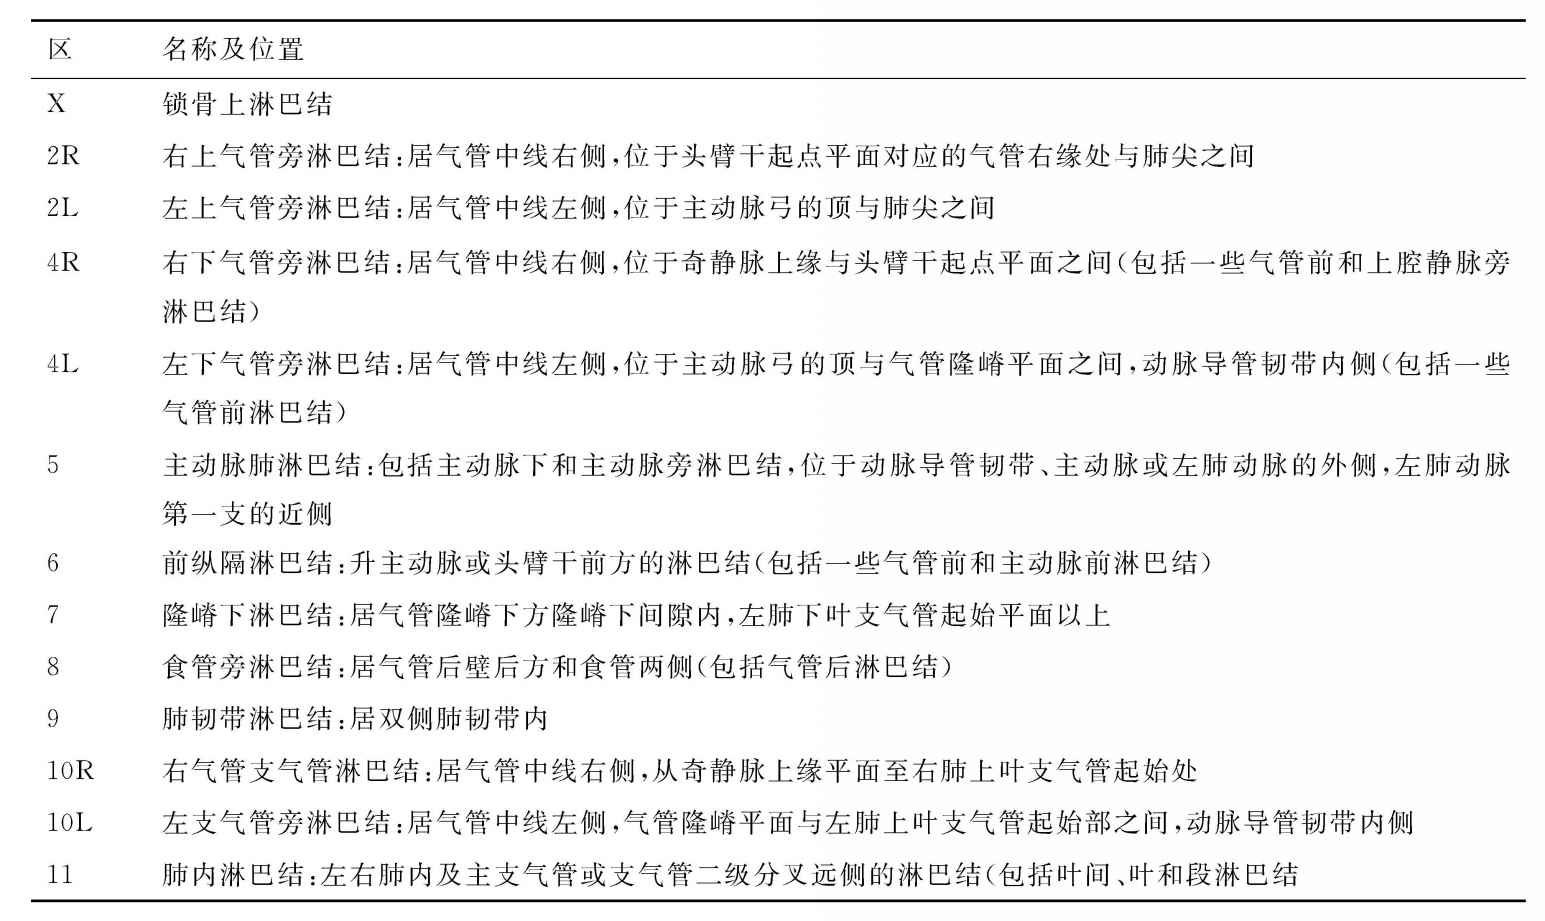
\includegraphics[width=\textwidth,height=\textheight,keepaspectratio]{./images/Image00181.jpg}
\end{table}

\begin{figure}[!htbp]
 \centering
 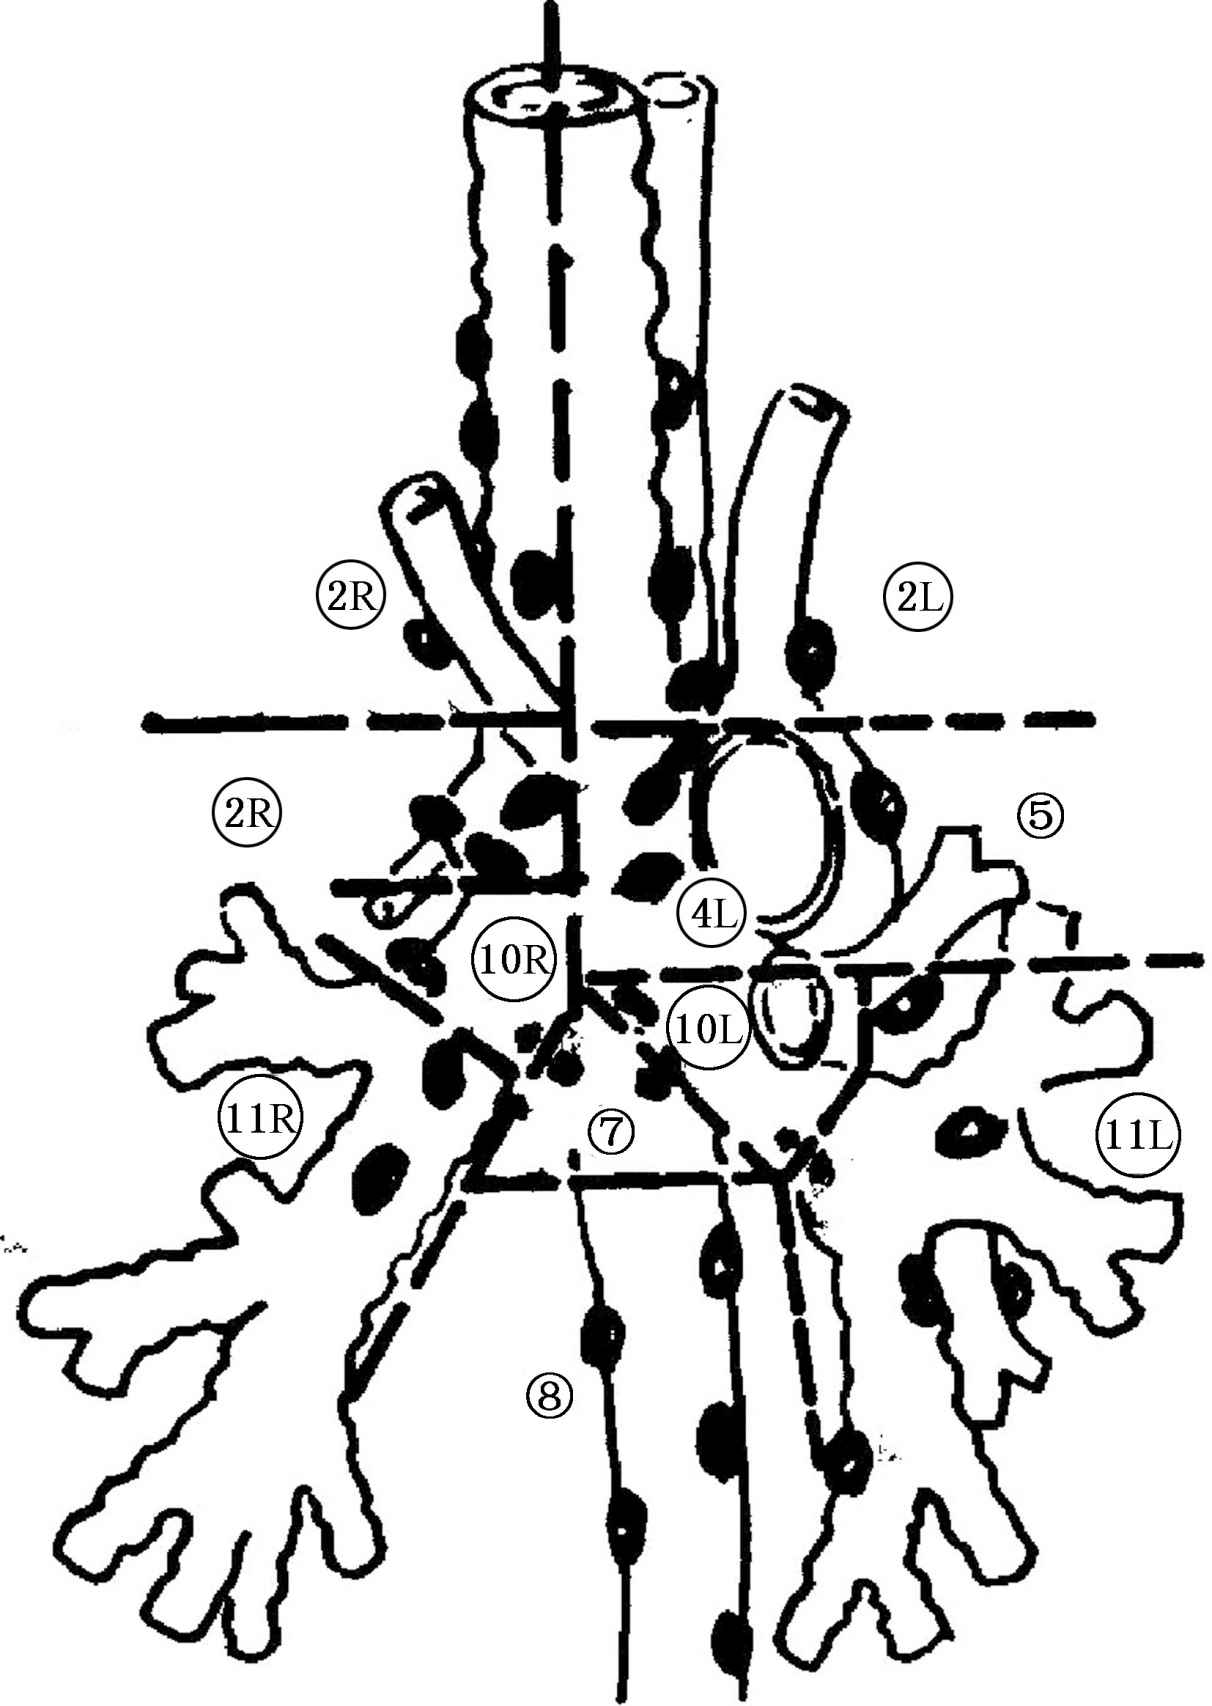
\includegraphics[width=.7\textwidth,height=\textheight,keepaspectratio]{./images/Image00182.jpg}
 \captionsetup{justification=centering}
 \caption{胸部淋巴结分组}
 \label{fig9-1}
  \end{figure} 

了解其分区对掌握肺癌的淋巴转移、术前分期和预后等均有重要作用。肺癌的淋巴转移可分为3站:第1站(N1)为10、11区;第2站(N2)包括2、4、5、6、7、8和9区;如果侵及斜角肌淋巴结或更远的淋巴结,则为远距离转移,即第3站(N3)。10区和4区被认为是预测肺癌可切除性和生存率的关键。

在纵隔不同部位淋巴结数量和大小有差异,如头臂静脉区域可<5mm,而在主-肺动脉窗、气管前、下气管旁、隆突下通常为6~10mm,心包旁正常人极少能发现淋巴结。在亚段支气管尚有淋巴结,向外是否有淋巴结尚有疑问。

淋巴结的测量以短径为标准。如≥1.5cm可考虑为病理性,≤1cm可考虑为正常,而在1.1~1.4cm之间则不能确定是否为异常。>2.0cm时以恶性肿瘤相对常见。

此外,正常腋窝淋巴结可含脂肪,甚至形成一个有包囊的、淋巴组织萎缩的肿大淋巴结。含脂肪者明显大于不含脂肪者,最大者长径可达3.5cm,故以腋窝淋巴结大小判断有无转移或良、恶性并不可靠。

\subsection{左右肺动脉及分支(见表\ref{tab9-2})}

\begin{table}[htbp]
\centering
\caption{左右肺动脉的分支}
\label{tab9-2}
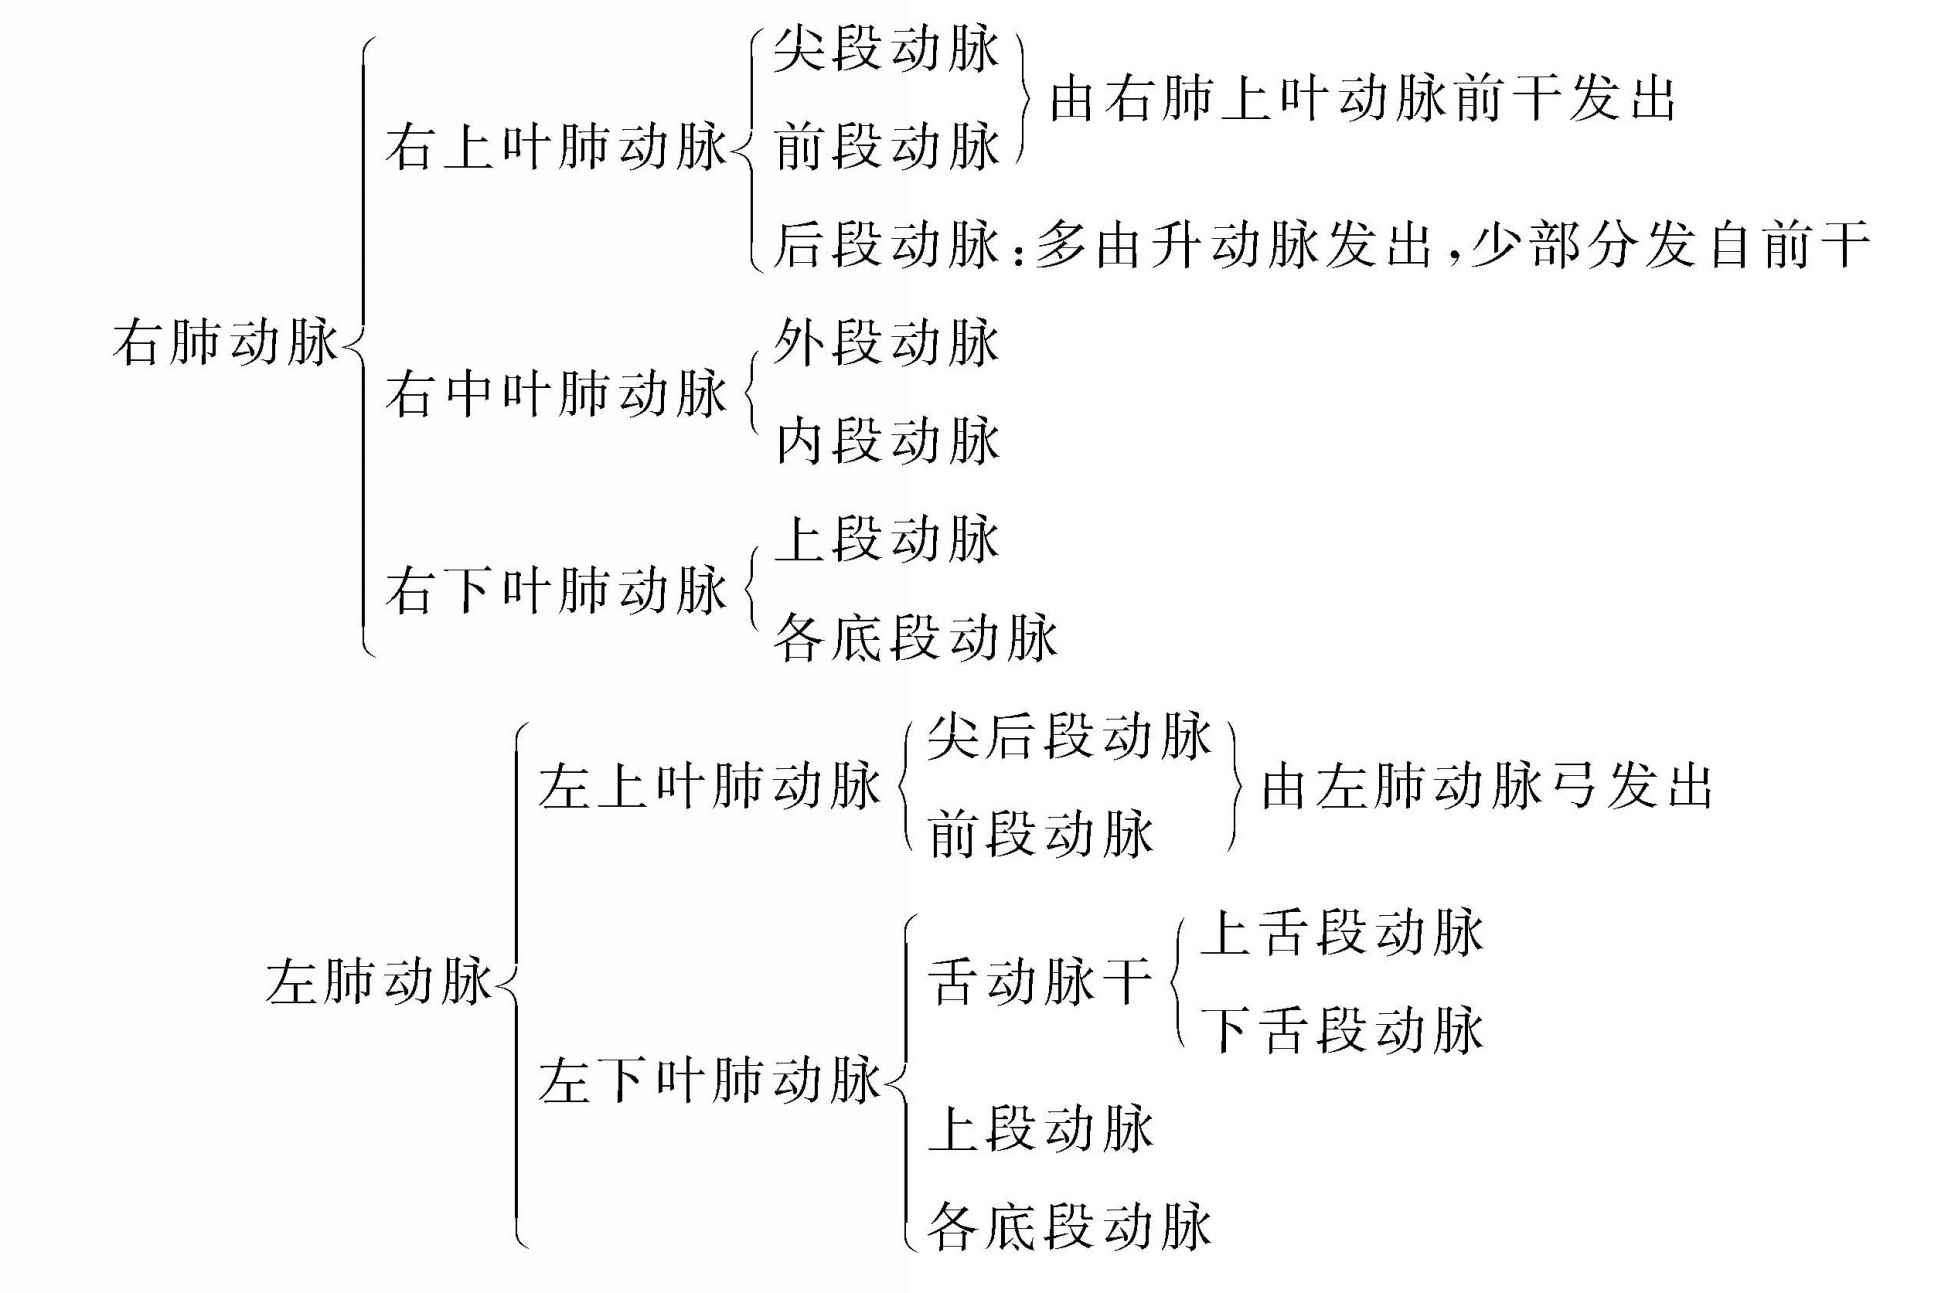
\includegraphics[width=\textwidth,height=\textheight,keepaspectratio]{./images/Image00183.jpg}
\end{table}

1.右肺动脉:分为右肺上叶、中叶和下叶肺动脉。右上叶肺动脉与右中叶肺动脉之间的一段动脉称为右肺叶间动脉。①右上叶肺动脉:可有1~4支,多为2~3支。右肺动脉入肺门后立即分出右肺上叶动脉(前干),在上叶支气管之前又分为尖段动脉(1~3支)和前段动脉(1~4支)。后段动脉(1~3支)17.3%发自前干,42%发自前干和升动脉,40.7%发自升动脉。升动脉(即后回归动脉)发自叶间动脉,81%分布于后段。②右中叶肺动脉:叶间肺动脉至中间支气管的右侧又分出1~3支(多为2支)中叶肺动脉,分为外段动脉和内段动脉。③右下叶肺动脉:可有3~8支(多为4~6支),肺段动脉的分支类型复杂。肺动脉转向右下叶支气管的外后方分出下叶背(上)段动脉,然后向下称为基底干动脉,再由其分出各底段动脉。

2.左肺动脉:左肺动脉跨越左主支气管向后,绕到上叶支气管后方,称为左肺动脉弓。再向下易名为左肺下叶动脉(故舌动脉干属左肺下叶动脉的分支)。①左上叶肺动脉:不形成总干,均是些短小的分支。尖后段动脉(以2支居多)和前段动脉(多为1支)发自左肺动脉弓。②舌动脉干:由左下叶肺动脉在斜裂处发出舌动脉干(多为1支),再由其分出上、下舌段动脉。③左下叶肺动脉:在上叶支气管的后方向下行走,其后上方的分支是背(上)段动脉(以单干2分支型多见,在舌动脉干稍上方发出),再向下分为各底段动脉。

\subsection{左右肺静脉及分支}

肺静脉有段内支和段间支两种属支。段内支常行于亚段间或更细支气管间;段间支行于肺段之间,引流相邻两肺段的静脉血。两肺的静脉最后汇集成4条肺静脉,均位于肺根的前下部,从两侧穿过心包进入左心房。肺静脉的变异较多,其最常见的分支形式见表\ref{tab9-3}。

\begin{table}[htbp]
{\centering
\caption{左右肺静脉的分支}
\label{tab9-3}
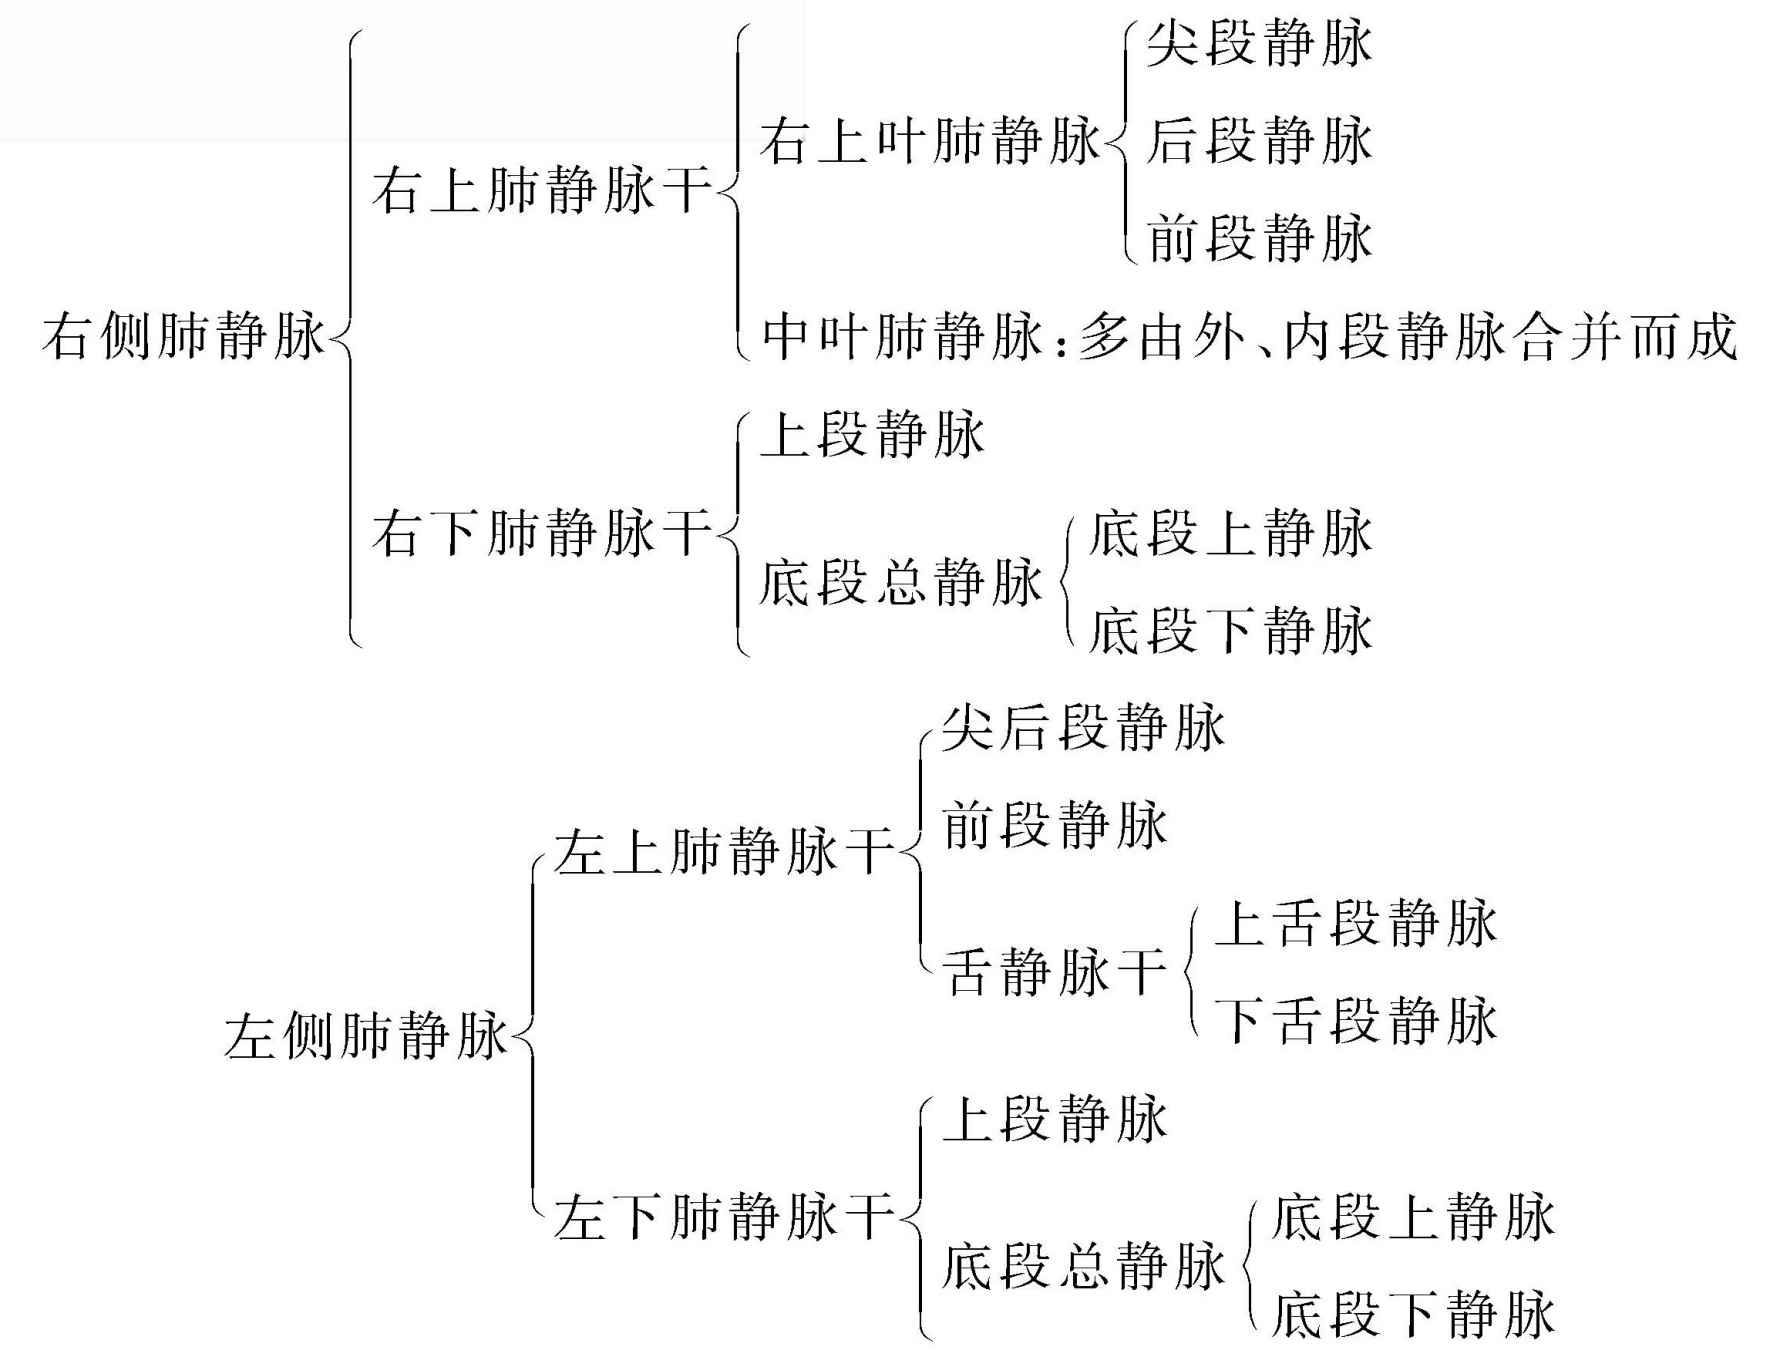
\includegraphics[width=\textwidth,height=\textheight,keepaspectratio]{./images/Image00184.jpg}}

{\small
注:(1)底段上静脉多由前、外底段静脉合并而成。

(2)底段下静脉多由后底段静脉形成;或由前底段静脉形成底段上静脉,外、后底段静脉形成底段下静脉。

(3)内底段静脉其注入处无一定规律。

左下肺静脉的汇合形式大致同右下肺静脉。
}

\end{table}



\subsection{肺动脉和肺静脉的相对位置关系}

总的来看,各个肺叶内支气管、肺动脉与肺静脉三者的相互关系是:①肺动脉与支气管在分支数目和形式上相互一致者甚少,但肺动脉的分支总是伴随相应的支气管从纵隔走向肺外围,且多位于同名支气管的前外侧或上方。②肺静脉居段间,与支气管一致者更少,肺静脉的走行多不与支气管并行且变异较常见,常位于同名支气管的后内侧或下方。③各基底段静脉相对同名支气管呈中心区分布,而同名动脉呈周围区分布。④左肺上叶由于动脉变异多,故支气管、肺动脉支、肺静脉支在分支上完全一致者基本没有,尤以尖后段变异较多,前段次之,舌段比较稳定。

\subsection{第二肺门及第三肺门}

1.肺门:又称为第一肺门、肺根,是肺与纵隔的通道,由支气管、血管(肺动脉、肺静脉、支气管动脉、支气管静脉)、淋巴管和神经被结缔组织包绕所构成。肺根内主要结构的排列:①从前向后:依次为上肺静脉、肺动脉、主支气管和下肺静脉。②自上而下:左侧依次为肺动脉、主支气管、上肺静脉和下肺静脉;右侧依次为上叶支气管、肺动脉、中下叶支气管、上肺静脉和下肺静脉。左右下肺静脉均位于肺根的最下方。

2.第二肺门:肺叶支气管、动脉、静脉、淋巴管和神经出入肺叶之处。

3.第三肺门:肺段支气管、动脉、静脉、淋巴管和神经出入肺段之处。

\subsection{右肺门的CT表现}

1.右尖段支气管水平:也相当于气管隆突水平。右尖段支气管呈小环状透亮影,伴随2个血管断面,右肺动脉的尖支位于其前内侧,右上肺静脉的后支位于其后外侧。

2.右主支气管水平:右上叶支气管从右主支气管侧面发出,通常平行向外延伸1~2cm,分出向前外走行的前支和斜向后上的后支。右主支气管前方是右上肺动脉,其直径与右主支气管横径相近,右上肺动脉的前、后支分别位于其伴随支气管的内侧。右上叶前、后两支气管夹角处之圆形或卵圆形影即为右上叶后段静脉。右上肺尖、前段静脉位于右上肺动脉前支与上腔静脉之间。

3.中间段支气管水平:右下肺动脉离开纵隔后先位于中间支气管前方,然后向下转到中间支气管外侧。在中间支气管上部层面,有时可见右上肺静脉的尖支和前支在中间支气管的前外侧汇合,后支位于其外侧。在中间段支气管下部水平,可见两根静脉汇合组成肺门前部分。右下肺动脉和静脉周围没有淋巴结显示。

4.中叶支气管水平:右中叶支气管发自中间段支气管并向前、外、下移行。右下肺动脉位于右中叶支气管与右下叶背段支气管夹角内。右中叶支气管外侧是中叶肺动脉,其内侧是右中叶肺静脉(但仅有50%显示)。

5.基底支气管或右下肺静脉水平:显示2~4个基底支气管断面,并可见伴随的基底动脉分支。右下肺静脉向内横行进入左房。

\subsection{左肺门的CT表现}

1.左尖后支气管水平:这一水平略高于右肺门对应的第一层面。左尖后支气管呈小环形影,有时可见两个分开的尖亚段和后亚段支气管分支。左尖后支气管内侧是左上肺动脉分支,其外侧为左上肺静脉后支。

2.左肺动脉水平:左肺动脉呈卵圆形影突出于纵隔左侧,其后方为降主动脉。尖后支气管断面位于左肺动脉外侧且几乎紧贴。左肺动脉内侧可见左主支气管。左上肺静脉位于尖后支气管的前内侧。

3.左上叶支气管水平:相当于右中间段支气管水平。大多数人显示左上叶前段支气管向前略向外延伸,其前内侧可见左上肺静脉和1~2个肺动脉分支呈分叶状致密影。左下肺动脉位于左上叶支气管后方。左舌叶支气管大多平行于左上叶前段支气管,但位于其下方。左上肺静脉位于左上叶前段支气管或左舌叶支气管内侧。

4.左下叶支气管层面:左下叶支气管多呈卵圆形断面影。其前壁大多与肺相邻,其后壁可见下叶背段支气管分出,左下肺动脉在其外侧呈分叶状或卵圆形致密影。

5.左基底支气管或左下肺静脉水平:与右侧相似,各基底支气管断面外侧可见左下肺动脉分支,左下肺静脉横行进入左房。

\subsection{肺叶和副叶}

右肺分为上、中、下三叶;左肺分为上、下两叶(左肺上叶相当于右肺上、中叶之和)。各叶之间都有叶间胸膜分隔,称为叶间裂。

右肺有两个叶间裂:①主裂(斜裂):它的起点约与第五肋骨后端同高,向前下多在前肋膈角后方2~3cm处与膈相交,很少止于前肋膈角。②横裂(水平裂):始于斜裂的中部、肺门的中点,水平向外达侧胸壁,水平裂内端较固定,外侧端偏上或偏下1~2个肋间隙。

左肺通常只有斜裂,其后端起点约在第四肋骨后端水平,前下端亦较右侧偏后。

叶间裂并非都是完整的。斜裂约有半数不完整。有学者报告右侧斜裂上半部70%分隔不完全,下半部47%分隔不完全;左侧斜裂上半部40%分隔不完全,下半部46%分隔不完全。水平裂分隔不完全更常见,通常不到达肺的纵隔面,分隔不完整者达94%。分隔不完整的叶间胸膜距离纵隔面和肺门的距离,最浅的可仅自肺的表面进入1~2cm。在分隔不完全的部位,两叶之间的肺组织相互密切沟通。

额外的胸膜裂(副裂)深入肺段之间,把肺段部分或完全的与其他肺段分隔开来,形成了副叶。有人统计高达50%。副裂可很浅,亦可伸入达肺门。常见的副叶有以下4个:

1.奇叶:系胚胎发育时奇静脉异常移行,将右肺上叶于肺尖处分隔成为两部分,并使局部的脏、壁层胸膜随之陷入,上肺叶的内侧部分即为奇叶(图\ref{fig9-2})。其大小随奇静脉的位置而异。奇副裂有2层脏层和2层壁层胸膜构成,由右肺尖部向内向下达肺门。奇叶发生率为0.5%。

\begin{figure}[!htbp]
 \centering
 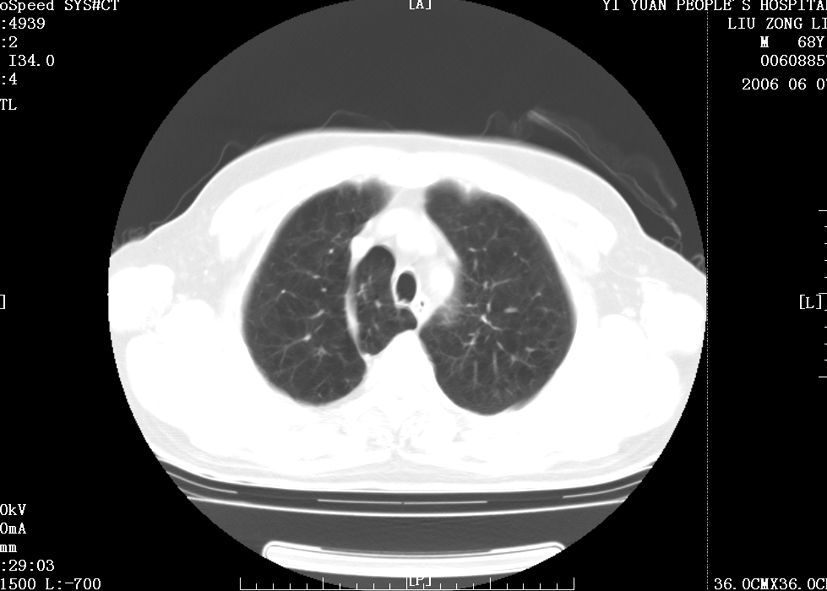
\includegraphics[width=.7\textwidth,height=\textheight,keepaspectratio]{./images/Image00185.jpg}
 \captionsetup{justification=centering}
 \caption{奇叶\\{\small 右肺尖段可见弧形奇静脉裂}}
 \label{fig9-2}
  \end{figure} 

2.下副叶:亦称为心后叶。系由下叶内底段形成,下副裂呈弧形,起自膈面,由外下方行至内上方。下副叶呈尖端指向肺门的楔形,是支气管扩张和先天性肺囊肿的好发部位。下副叶以右侧多见,发生率为30%。

3.后副叶:由下叶背段形成,多见于右侧。后副裂似为水平裂向后延伸而成。

4.左中副叶:相当于右肺中叶。左横副裂把舌叶与上叶其他部分分隔成为独立的肺叶,即左中副叶。发生率为8%。

\subsection{叶间裂的CT表现及肺叶的分辨}

1.叶间裂:①斜裂:在常规CT上呈无血管带或区,但薄层扫描或HRCT能清晰显示它呈细线状或条状高密度影。由于左肺斜裂较右侧陡直,故在由上向下的扫描中左侧斜裂先出现,且斜裂的位置由肺野的后方逐渐向前方推移。斜裂的形态在肺门上方层面上,内侧高于外侧,呈凸面向后的弧形;在肺门层面上,内、外侧几乎等高,稍呈内侧后凸外侧前凸的波浪状;在肺门下方层面上,外侧高于内侧,呈凸面向前的弧形。②水平裂:常规扫描时,显示为较斜裂更宽的无血管带,往往与其后方的斜裂共同构成类圆形或底在肺表面的楔形乏血管区。薄层扫描或HRCT也常表现为线样致密影。

2.当发现肺不张或水平裂不易确定时,区别右上叶与右中叶比较困难。但有学者认为:CT尤其HRCT上右上叶前段的内亚段支气管位于其伴随肺动脉分支的外侧;而右中叶外侧段的内亚支或内侧段的上亚支、下亚支均位于其伴随动脉的内侧。依此判断右上叶和中叶,准确率可达100%。

3.“左上叶”与“左舌叶”的位置不易判断,可根据各自支气管的位置及走行方向大体估计。

\subsection{肺段}

右肺有10个肺段,左肺有8个肺段。每个肺段有与其名称相应的单独支气管。肺段之间正常情况下没有清楚的边界,无胸膜分隔。只有在病理情况下形成实变或不张时,才能看清楚边界。肺段通常呈圆锥状,尖端指向肺门,底部朝向肺外围。各肺段命名如下:

1.右肺:①S\textsubscript{1} (尖段)、S\textsubscript{2}
(后段)、S\textsubscript{3} (前段);②中叶:S\textsubscript{4}
(外段)、S\textsubscript{5} (内段);③下叶:S\textsubscript{6}
(背段亦称为上段)、S\textsubscript{7} (内底段)、S\textsubscript{8}
(前底段)、S\textsubscript{9} (外底段)、S\textsubscript{10}
(后底段)。

2.左肺:①上叶上部:S\textsubscript{1+2} (尖后段)、S\textsubscript{3}
(前段);②上叶舌部:S\textsubscript{4} (上舌段)、S\textsubscript{5}
(下舌段);③下叶:S\textsubscript{6}
(背段亦称为上段)、S\textsubscript{7+8}
(前内底段)、S\textsubscript{9} (外底段)、S\textsubscript{10}
(后底段)。

\subsection{CT图像上各肺段的确定}

CT
图像上各肺段之间无明确边界,肺段支气管与相应肺动脉、肺静脉的相对位置关系是识别肺段的基础。一般先寻找斜裂及水平裂,将肺叶分开,再以各叶内的管道来确定肺段。确定肺段的主要依据是肺段支气管,它位于肺段的中心;肺静脉段间支位于相邻的肺段之间,构成肺段的边缘,是划分肺段的标志。

\subsection{肺血管的CT表现及肺血坠积效应}

1.在常规CT上:①一般难以显示段以下支气管,只有当其周围肺实变,本身病变引起扩张或壁增厚时才能显示。②肺野内显示的血管影代表肺动脉和肺静脉,多呈树枝状分支,且从肺门至外周逐渐变细,距肺边缘或叶间裂1~2cm处不能显示而形成无血管区。一般来说,肺段动脉紧密伴行同名支气管,多位于支气管的前、外或上方;肺段静脉主干则位于同名支气管的后、内或下方。

2.在HRCT上:①支气管影由于其扫描角度不同而呈环状、椭圆形、轨道状或锥状,壁光整。正常支气管壁的厚度相当于其管径的1/6~1/10,因此当管径<2~3mm或胸膜下2~3cm内的正常支气管在HRCT亦不能显示。②肺门周围的大血管分支呈圆形或卵圆形。肺动脉影通常与支气管影伴行,且管径与伴随的支气管管径大致相等。肺野的血管影多呈点状或小卵圆形,分布均匀,疏密适中。

3.肺血坠积效应:由于肺重力的作用,靠近扫描床的肺血管要略大于远离部分的肺血管。当肺容积较大时,这种差异很小。而当肺容积小时,这种差异就较显著,越靠近扫描床处越密集,甚至表现为肺承重部位胸膜下新月形或弧形密度增高区或实变,这种现象称为肺血坠积效应。它可能是承重部肺组织的相对膨胀不全所致。改变体位或增大肺容量时消失或明显减轻。

\subsection{肺泡孔和Lambert管}

每个肺叶内由50~80个肺小叶组成。每个肺小叶之间由结缔组织、血管(主要是肺静脉)、淋巴管及神经纤维构成小叶间隔。肺小叶呈锥形的多面体,成人底部1cm左右,高约1cm,近肺外周者可高达2~3cm。每个小叶中部有一支小叶支气管(属细支气管),小叶动脉伴随小叶支气管进入肺小叶。每支肺小叶支气管又分出3~5支末梢(终末)细支气管。

终末细支气管继续分出几组一、二、三级呼吸性细支气管,以后再分为肺泡管、肺泡囊、肺泡。从一、二、三级呼吸性细支气管开始直至肺泡称为肺腺泡(又称呼吸小叶、初级小叶),其直径4~6mm,是X线和CT病理改变的基本单位。所以,每个肺小叶由3~5支末梢细支气管及其远端所续的多个腺泡(呼吸小叶)组成。但腺泡之间无明显界限,HRCT无法显示其结构。

肺泡与肺泡之间有交通孔,直径约10~15μm称肺泡小孔(Kohn孔)。另外,Lambert还描述了肺泡与大于末梢细支气管的细支气管之间还存在着通道称为
Lambert管。以上两者均具有肺组织间侧支通气作用,可防止发生肺不张,但也是病变扩散的通路。

\subsection{肺小叶的HRCT表现}

肺小叶由小叶间隔、小叶核心和小叶实质组成。在HRCT上呈多边形或截头锥体形,底位于肺表面侧、尖向肺门。HRCT可显示直径0.2mm以上的肺小叶结构,正常小叶内终末细支气管壁厚约0.1mm,小叶间隔厚0.1mm,故无法显示。

1.小叶间隔:正常人的小叶间隔往往不能显示,即便能显示也不及离体标本的清楚。它表现为薄而均匀的线状致密影。边长约1~2.5cm,厚约0.1mm。小叶间隔的数目多少不等,以上、中(舌)叶胸膜下最多,下叶次之,各肺叶近肺门区最少。小叶间隔内的静脉多可显示,直径约0.5mm,表现为点状或逐渐变细的线样高密度影,有伸向胸膜的趋势。

2.小叶核心结构:主要由小叶动脉和细支气管组成,它们的直径约1mm。小叶内终末支气管及其动脉直径约0.5~0.7mm。在离体标本上可显示上述结构,在活体标本上仅可显示小动脉而难以显示细支气管,可能与运动伪影和体壁干扰有关。HRCT上可见这些小叶动脉呈线状、分支状和点状软组织影,距小叶间隔3~5mm,但只能显示至胸膜下5~10mm处。

3.小叶实质:即腺泡(呼吸小叶或初级肺小叶)。HRCT可见其内的点状血管断面,但不能显示其完整的轮廓和呼吸性细支气管。

有学者将肺分为外周的皮质和中央的髓质,有助于某些疾病的诊断。其解剖及HRCT的依据如下:①皮质:由1~2排分化较好的周边肺小叶组成,相当于距胸膜面3~4cm以内。HRCT皮质小叶间隔相对容易显示,血管较细,但支气管常难以显示。②髓质:靠近肺门周围,肺小叶即小叶间隔发育多不完全。血管和支气管较粗,HRCT能清晰显示,但多无法显示其完整的小叶结构。

\subsection{终末细支气管}

1.中央气道:定义为直径>2~3mm的气道。

2.外周气道:通常称为细支气管,直径<2~3mm。

3.小气道:直径≤3mm的气道,绝大多数为呼吸性细支气管。

4.细支气管:管壁缺乏软骨的小气道,最大直径约3mm,壁厚约0.5mm。

5.终末细支气管:是指不参与气体交换的最后一级纯粹导气道,直径0.7mm,发出呼吸性细支气管,一条或多条呼吸性细支气管供给一个腺泡。

\subsection{胸膜腔和胸腔}

1.胸膜:是覆盖于肺表面和胸壁内面的薄层浆膜。可分为:①脏层胸膜:被覆在肺表面。②壁层胸膜:衬覆于胸腔各壁内面,按部位分为肋胸膜、膈胸膜、纵隔胸膜和顶胸膜。

2.胸膜腔:是由脏、壁两层胸膜在肺周围形成的腔隙。两层胸膜在肺门部移行汇合,包绕而成两侧互不相通的胸膜腔,宽约18~20μm。内有少量浆液。

3.胸腔:由胸廓与膈围成。胸腔内容为3部分,即左右两侧的胸膜腔和肺,中间被纵隔占据。

人的脏层胸膜较厚,大约100μm,约为壁层胸膜的5倍。

壁层胸膜与脏层胸膜最大的区别是壁层胸膜的间皮细胞间有许多微孔,这些微孔通常成簇或成组分布,与周围淋巴间隙相接,是胸膜腔内液体、蛋白质和细胞成分的溢出孔道。

生理胸液是由胸腔尖顶区的壁层胸膜产生,而由胸腔最低区主要是横膈面和纵隔面壁层胸膜上的淋巴微孔吸收。脏层胸膜对胸液的形成和重吸收几乎不起作用。正常情况下胸液量约为0.3ml/kg,为低渗性(含蛋白10g/L)。

\subsection{肋间线}

1.胸膜外脂肪:在壁层胸膜外,存在一个以脂肪为主的间隙被称为胸膜外脂肪、胸膜外间隙、胸膜外肋骨下组织等,多称为胸膜外脂肪。它是位于壁层胸膜与肋骨最内肌和胸内筋膜之间的脂肪组织,通常厚度<2mm。

2.肋间线:在正常人的HRCT上,两侧相邻肋骨段之间的肺与胸壁交界处可见一条1~2mm厚的软组织线称为肋间线(亦称为肋间带),是脏层胸膜、壁层胸膜、胸膜腔内生理液体、胸内筋膜和肋间最内肌的投影。正常人的这条线主要代表肋间最内肌,因为它是这几层中最厚的结构。肋间线与外层肋间肌之间可见肋间脂肪层。

肋间肌并不覆盖肋骨表面,因此肋骨面不能看见肋间线。虽然胸膜及胸内筋膜覆盖肋骨面,但它们太薄且紧贴致密的肋骨面,即便HRCT也无法显示。因此如果肋骨面上看见线状影,通常提示胸膜增厚或积液。

在椎体旁区没有肋间肌,但HRCT也能显示此处肺表面的线状影,它只代表脏、壁层胸膜及胸内筋膜,因此这条线比肋间线细的多,且不很清晰。椎旁肋间静脉丛位于胸膜外且不凸向肺表面可与胸膜增厚区分。

此外,在HRCT还可见在前部的肋骨、肋软骨和胸骨后有一纤细的带状影,为胸横肌的投影。

\subsection{胸壁的CT表现}

胸壁主要由骨结构和肌肉组成,胸壁的脂肪可使胸壁肌肉详细显示。①肋骨呈条带状,可见其皮质和髓腔。因在同一层面不能显示肋骨的全长,故肋骨的序数和详细形态不易判断。肋骨的斜面形态可类似骨破坏。②胸椎位于胸廓后部。③肩胛骨位于后胸壁两侧,左右对称。④在肺尖层面有时第一肋骨近胸骨端下缘有一骨性突出,类似肺内结节。⑤在前胸壁第五肋以上有较厚的胸大肌和后方较薄的胸小肌。第七肋以下有腹直肌和腹外斜肌。最前方为女性乳房,可见皮肤、皮下组织和乳腺。⑥腋窝部有丰富的脂肪,其内淋巴结增大易发现。⑦后胸壁有斜方肌、菱形肌和胸椎棘突周围肌群等。

\subsection{腰肋三角}

膈由中心腱及肌肉组成。中心腱为圆顶状膜状结构。肌肉组织根据其起始部位分为以下3部分:

1.腰椎部:①内侧角形成左、右侧膈脚。右侧膈脚起自L\textsubscript{1~4}
椎体处;左侧膈脚起自L\textsubscript{1~3}
椎体处。两侧膈脚呈弧形向前上走行至主动脉裂孔及食管裂孔,由一弓形韧带连接两侧膈脚构成主动脉裂孔的前缘,而膈脚构成裂孔的侧缘。主动脉裂孔位于T\textsubscript{12}
前方,食管裂孔位于主动脉裂孔的左前方T\textsubscript{10}
水平,下腔静脉裂孔在主动脉裂孔的右前方之中心腱处。②外侧角起自内、外侧弓状韧带。

2.肋骨部:起自第7~12肋软骨。

3.胸骨部:位于剑突背面及腹直肌鞘后部。

膈肌在胸骨两侧和第七肋骨附着点之间各有一三角形间隙,局部肌肉和腱膜组织较少,称胸肋三角或胸骨旁裂孔(Morgagni孔)。膈肌两后外侧部也各有一个仅有筋膜而无肌肉的三角区,称为腰肋三角或胸腹膜裂孔(Bochdalek孔)。

\subsection{膈的CT表现}

1.前膈肌:即肋膈肌。附着于剑突及两侧肋软骨上,CT表现有3类:①呈光滑的或轻微的波浪状线影,线影两侧衬有脂肪,略向后凹并汇合于中线。这一典型表现在剑突水平易显示,也是最常见的一种表现类型。②两侧膈肌呈线状影,但于中线处不连续。③呈不规则的、成角或边缘不清楚的宽肌肉带影。

2.膈脚:它是膈肌与脊柱前纵韧带相连续的肌腱结构,它们与脊柱之间有椎前和椎旁脂肪。多数表现为椎体两侧弧形软组织影,可以厚度一致,也可局部增厚呈卵圆形或圆形软组织影。右侧膈脚常厚于左侧。膈脚吸气时比呼气时厚。

3.弓状韧带:它是覆盖腰大肌、腰方肌和胸膜筋膜的增厚部分,也是膈肌后部分的附着。CT表现与膈脚无明显界线,通常表现为膈脚向后外延伸的线状致密影,且有报道5%后膈肌附着处(弓状韧带)可呈结节状,但与线状后膈肌影相连续,可两侧对称或不对称,勿误为增大淋巴结。

4.膈肌裂孔:①主动脉裂孔内有降主动脉、奇静脉和半奇静脉、胸导管等结构穿过。②食管裂孔:有食管和迷走神经通过。③下腔静脉孔、胸骨旁裂孔、胸腹膜裂孔CT不能显示。

此外,膈的表面有时可见线状影,是胸膜包裹的膈神经或膈上动脉及静脉的影像。

\section{呼吸系统疾病的基本CT表现}

\subsection{气管和支气管病变}

1.气管腔内软组织肿物:可呈息肉状、结节状和肿块状。①良性者边缘光滑,多在2cm以下。可见于乳头状囊腺瘤、纤维瘤、平滑肌瘤、错构瘤和软骨瘤等。②恶性者边缘光滑或不光滑,基底部较宽。③黏液栓呈液体密度,咳嗽后消失。

2.气管、支气管狭窄和阻塞:①局限性:多为肿瘤,恶性者引起管壁增厚。②弥漫性:可累及气管、主支气管、肺叶和肺段支气管,见于复发性多发性软骨炎、支气管结核、肺淀粉样变等。阻塞的原因可为腔内阻塞和腔外压迫,腔内原因除肿瘤外还有异物、分泌物、凝血块、肉芽组织、水肿、痉挛性收缩等;腔外病变压迫常见于肿大的淋巴结、肿瘤等。不完全阻塞可引起局限性、一侧性、两侧性肺气肿;完全阻塞可引起一侧性不张及肺叶、肺段、肺小叶不张。

3.气管、支气管管壁增厚:正常气管、主支气管的管壁厚度为1mm左右。恶性肿瘤常为局限性、环形增厚,合并管腔狭窄、阻塞和管外肿块。复发性多发性软骨炎增厚广泛。

4.气管、支气管管腔增宽:正常气管管腔宽度为15~20mm,男性平均19.5mm,女性平均17.5mm。主支气管宽右侧平均为15.3mm,左侧为13.0mm。巨气管支气管症可使气管及左、右主支气管增宽。肺段以下支气管腔增宽见于支气管扩张症。

\subsection{外周小气道病变}

外周小气道病变即细支气管的支气管壁增厚及管腔扩大病变。其HRCT表现如下:

1.直接征象:①细支气管壁增厚及管腔扩大表现为充气扩张、分叉状、环形或管状结构影。②当气道由于腔内隆起或黏膜下及细支气管周围纤维化而阻塞时,常可见呈结节、线状或分叉状影。

2.间接征象:受累小气道引起远端肺实质的病变为外周气道病变的间接征象。①空气潴留:小气道的闭塞、狭窄的另一常见表现为空气滞留或过度充气,可产生马赛克表现,称为空气滞留征。“马赛克样”表现是由以肺叶、段或亚段为单位的肺组织透亮度增加(肺灌注下降)与邻近灌注正常或轻度灌注增加的肺组织所形成。②小叶中心型肺气肿:多由吸烟引起,最先发生于双上肺。③小叶中心气腔结节:外周小叶中央小结节状实变是其非特异性间接征象之一。这些模糊的小结节见于细支气管周围炎,呈圆点状、磨玻璃样改变,大小<1cm。④亚段性肺不张:小气道远端发生亚段的肺膨胀不全时,HRCT呈典型的楔形磨玻璃影。

\subsection{肺间质的概念}

具有气体交换功能的腺泡,包括一、二、三级呼吸性细支气管、肺泡管、肺泡囊、肺泡统称为肺实质。支气管、血管、淋巴管周围和小叶之间的疏松结缔组织,以及支气管、血管、淋巴管及肺泡壁的胶原纤维、弹力纤维及嗜银纤维统称为肺间质。

从宏观上讲,肺实质病变主要侵及肺泡腔,以肺泡、腺泡(呈花蕾状)、小叶乃至大叶的分布方式存在;以肺间质病变为主的病变表现为条索状、网状、蜂窝状以及较广泛的小颗粒状阴影,有时网状阴影与颗粒状阴影同时存在。

\subsection{肺实质的实变}

肺实质的实变是指肺泡内的空气被病理性物质所代替。这些病理物质可以是炎性渗出物、血液、水肿液,也可以是增生的肉芽组织等。

1.炎性渗出液(可为浆液性、脓性和纤维素性)所引起的实变,由于渗出液可以通过肺泡孔向邻近肺泡蔓延,因此病变区与正常肺组织间并无截然分界,呈相互移行状态。影像学呈大片状、小片状边缘模糊之高密度影,亦可表现为以叶间胸膜为界的全叶性实变。渗出性病变吸收过程中,失去均匀致密的特点。

2.肺出血和肺泡性肺水肿所形成的实变形态与肺炎相似,但其变化较急性肺炎更快,适当处理可在数小时或1~2日内完全消失。

3.肉芽组织增生引起的实变在病理上局部以巨噬细胞增生为主,形成境界清楚的肉芽肿,主要见于结核、真菌、寄生虫等。影像学见病变多呈腺泡结节状,没有融合趋势。

炎性渗出常自肺的外周向肺门方向扩展。当病变扩展至肺门附近时,较大的含气支气管与实变的肺组织形成对比,在实变的肺组织中可见到含气的支气管影,称为空气支气管征。对病变周围渗出较明显的病灶,尤其是双肺后部的病变,由仰卧位改为俯卧位CT扫描可明显增加该征的显示率。

\subsection{肺钙化病变}

钙化一般发生于退行性变性坏死的组织内。为组织遭受破坏时,局部有较多的脂肪酸分解出来,导致酸碱度的变化,从而使钙离子以磷酸钙或碳酸钙的形式沉积下来。钙磷代谢障碍引起血钙增高,亦可在肺内发生病理性钙质沉着。

钙化最多见于肉芽肿性病变(如结核、真菌病),还可见于肺癌、肺转移瘤。以钙化为影像学特征的疾病有肺泡微石症、原发或继发性甲状旁腺功能亢进、摄钙量过多、维生素D中毒等。含铁血黄素沉着及矽肺则出现较弥漫的肺内钙化样高密度灶,应注意鉴别。乙胺碘呋酮用药量过大亦可出现钙化样高密度灶,此时肝、脾密度亦常增加,有助于鉴别。

CT表现:钙化的形态多种多样,如层状、细颗粒状、结节状或无定形。在病灶中的部位亦各不相同。

\subsection{肺空洞与空腔}

\subsubsection{空洞}

是部分肺组织坏死液化经引流支气管排出所致。

1.空洞壁的分层:①虫蚀样空洞:洞壁由坏死组织所组成。②有壁空洞:洞壁主要由坏死组织、肉芽组织、纤维组织及薄层不张的肺组织所构成。如活动性肺结核洞壁由干酪坏死组织、肉芽组织及纤维组织所构成,在稳定期主要由纤维组织所构成。脓肿壁由坏死组织、肉芽组织及纤维组织所构成。癌性空洞壁由坏死组织、肿瘤组织及薄层不张的肺组织所构成。

2.空洞的影像学分类:可分为3类。①虫蚀样空洞:又称为无壁空洞,是大片坏死组织内产生的空洞,常多发。洞壁不规则,如虫蚀样,由坏死组织形成,见于干酪性肺炎。②薄壁空洞:洞壁薄,约为2~3mm以下。空洞多呈圆形,界限清晰,内壁光滑,一般无液平面,周围很少实变影。多为发生时间较久的空洞,常见于肺结核。③厚壁空洞:洞壁厚约3mm以上,形状不规则。空洞周围常有密度增高的实变区;内壁可凹凸不平,也可光滑整齐。多为新形成的空洞,见于肺脓肿、肺结核及肺癌。结核性者洞内多无或仅有少量液平面,而肺脓肿空洞内多有较明显的液平面。癌肿内壁呈结节状凹凸不平。

影像学下分析空洞时应注意:空洞的多少、大小、内缘、外缘、壁厚、内容物、周围组织改变、有无引流支气管、肺门的改变、胸膜的改变、动态变化等。如空洞直径<3cm者炎性病变多,>3cm的多是肿瘤;壁厚<4mm者常为良性病变,>15mm者多为恶性病变;引流支气管多见于肺结核;多发性空洞可见于血源性脓肿、转移瘤、淋巴瘤、肺结核等。

\subsubsection{空腔}

是肺的生理性腔隙呈病理性扩大所致,如肺大泡、含气肺囊肿及肺气囊等。空腔的壁较空洞薄,一般在1mm以下;一般无腔内液体,周围多无实变,但继发感染或由于感染性病变所致的空腔例外。

\subsection{肺结节和肿块}

肺部的孤立结节和肿块较常见,结节系指病灶直径≤3cm的病灶,但常统称为肿块。按其病因病理可分为两类:①瘤性肿块:分为原发和继发两种。原发又分为良性和恶性肿瘤;继发性多由血行转移而来。②非瘤性肿块:多见于炎性假瘤、结核瘤、肺内囊性病变、血管性病变等。

影像学在分析块状病变时应注意:肿块的大小、位置和分布、数目、形态、密度、边缘、周围肺野的表现,以及有无空洞、引流支气管、钙化、淋巴结增大及邻近胸膜改变等。尤其要注意有无空泡征、结节征、边缘分叶征、毛刺征、胸膜凹陷征、血管集聚征等肺癌的表现,并结合增强扫描表现及CT值的变化等予以综合分析和诊断。

HRCT的结节是指局限性、大小不等的圆形致密影。依结节大小分为大结节(>1cm)、小结节(<1cm)和微结节(≤0.7cm),亦有以<0.3cm者称为微结节。也可按结节边缘清楚、模糊或按结节位置(如随机分布、淋巴管周围分布、小叶中心分布)分类。

\subsection{肺纤维性病变}

肺的纤维性病变可分为局限性和弥漫性两类,有3种基本X线和CT表现:

1.范围较小的纤维性病变可表现为较为局限的索条状阴影,密度高、僵直。多见于肺结核与慢性炎症。

2.病变被纤维组织代替后,收缩形成密度高、边缘清楚的块状高密度灶。如病变范围大,累及1~2个肺叶,可使部分肺组织发生瘢痕性膨胀不全而形成大片状高密度灶,密度可不均匀;其内可见密度更高的索条状影及低密度的支气管扩张影。周围器官被牵拉移位。多见于慢性肺结核和矽肺。

3.弥漫性纤维性病变可广泛发生于肺间质内,表现为紊乱的索条状、网状或蜂窝状影。如为肉芽肿或尘肺等引起的肺纤维化,可表现为在网状阴影的背景上有许多弥散的颗粒状或细小的结节状阴影称为网状结节病变。

\subsection{弥漫性肺间质性病变}

\subsubsection{病因和分类}

包括水肿、炎症、纤维化、肿瘤等。CT影像为两肺广泛分布的肺间质结构的异常。又可分为间质纤维化和非纤维化间质病变两类。①肺间质纤维化疾病:包括多种慢性肺间质性疾病,常见的有特发性肺间质纤维化、慢性支气管炎合并的肺间质纤维化、结缔组织疾病性肺间质纤维化(类风湿关节炎、硬皮病、干燥综合征及系统性红斑狼疮等)、结节病、过敏性肺炎的终末期及尘肺等。除特发性肺间质纤维化外,其他特发性间质性肺炎所致的纤维化相对少见。②无纤维化的肺间质疾病:主要有间质性肺水肿和癌性淋巴管炎等。

\subsubsection{HRCT的CT征象}

1.小叶核心增大及小叶内间质增粗:①小叶核心增大:表现为小叶中心出现明显的点状或“Y”形影像,为小叶内支气管血管周围间质增厚所致。②小叶内间质增粗:表现为小叶内的线状、细网状、放射状影像,为小叶内细支气管血管周围间质和肺泡壁的间质增厚所致。常合并小叶间隔增厚。

2.小叶间隔增厚:表现为与胸膜垂直的一条或多条细线状影像,长约1~2cm。①光滑的增厚:通常提示间质水肿、弥漫性间质性病变的早期等;②串珠状的增厚:见于癌性淋巴管炎、淋巴瘤、淋巴管肌瘤病、结节病、煤尘肺;③粗细不均的增厚:提示间质纤维化。

总之,小叶间隔增厚可见于肺感染性疾病(病毒性感染、细菌性肺炎、卡氏肺囊虫肺炎、结核等)、肺水肿、肺肿瘤(如弥漫性肺泡癌、转移瘤、淋巴瘤、白血病、中央型肺癌阻塞性肺炎等)、导致纤维化的弥漫性间质性肺病。

3.肺长线影:呈2~5cm长的线状影,粗细较均匀,从肺野延伸到胸膜面。通常提示明显的间质纤维化,但有时与粗瘢痕影或盘状肺不张难以鉴别。

4.胸膜下线:表现为胸膜下1cm内与胸膜平行的弧线形影像,长1~10cm左右,多位于后部的肺段。其病理基础一般认为是细支气管周围的纤维化病变及肺萎缩。见于多种间质纤维化疾病。

5.支气管血管束异常:需结合其他征象综合分析。①边缘毛糙(界面征):支气管血管束周围有间质纤维化、小叶内间质增厚及蜂窝改变,均可使其边缘毛糙及不规则,称为界面征;②合并结节:见于癌性淋巴管炎、结节病及尘肺;③支气管壁增厚:多见于慢支;④支气管血管束均匀增厚、边缘光滑:见于间质性肺水肿。

6.蜂窝状影像:表现为多发集聚的囊腔,直径几毫米至1厘米,甚至几厘米(结缔组织病肺间质纤维化的囊腔多<3mm,直径>5mm者多见于特发性肺间质纤维化);多位于肺的外周和胸膜下,邻近胸膜常轻度肥厚,是晚期间质纤维化的表现,因失去气体交换功能故又称为终末肺。

7.牵拉性支气管扩张:发生在间质纤维化严重的部位,常与蜂窝肺并存,支扩呈不规则管状。末梢扩张亦可呈蜂窝状,但常合并不规则的支气管形态。

8.磨玻璃密度:见于特发性肺间质纤维化、结缔组织病等疾病的早期和活动期。

9.肺间质性结节(见后述)。

\subsubsection{病变的分布和动态变化规律}

1.病变的分布:小叶内间质增厚、小叶间隔增厚、胸膜下弧线影及早期蜂窝表现多分布于肺的边缘部位。这是由于这些征象的病理解剖基础均位于小叶范围内,且肺小叶在肺的外周部分发育完善。故要注意从肺的边缘部识别这些征象,尤其是早期病变。随着病变的进展,病变在肺内广泛分布。

2.动态变化:早期一般为小叶内间质增厚、小叶间隔增厚及胸膜下弧形影,病变进展可发展到蜂窝改变或牵拉性支气管扩张。①肺间质纤维化进展缓慢,一般1~2个月无明显动态变化。急性间质性肺炎可在1个月内有明显变化。②非纤维化的间质病变动态变化较快,间质性肺水肿可在数日内有显著变化,癌性淋巴管炎可呈进行性加重。

\subsection{弥漫性肺泡病变}

\subsubsection{病因}

该类病变表现为肺内广泛的肺泡实变影。主要见于各种病原菌(包括细菌、病毒、真菌和原虫等)引起的炎症、过敏性肺炎、肺水肿、休克肺、肺泡蛋白质沉着症等。主要病理改变为肺泡内充盈浆液性、脓性或血性等液体。

\subsubsection{CT表现}

1.病变的形态:①多叶、多段肺实变:病变范围广泛,大小不一。病变内可见含气支气管征。②磨玻璃密度:是指肺部阴影密度低而均匀,在其内可见血管影像。此征象即可见于肺泡性病变(如肺水肿、肺泡蛋白质沉着症、各种原因的肺泡炎、过敏性肺泡炎等),也可见于肺间质性病变的早期及活动期。

2.病变分布:一般按肺单位分布,即为腺泡、肺小叶、肺段或肺叶的实变。腺泡及小叶实变多沿支气管走行分布。有些肺泡病变在两肺融合成大片状影像。如病灶分布在肺野内、中带,其外带病变较少或正常,称为肺边缘透明带,此征象见于肺泡蛋白质沉着症及中央型肺水肿。

3.动态变化:一般较快,多在1~2周内病变有明显吸收或增大,见于急性炎症、肺水肿、肺出血性病变。腺泡状、小叶性影像可融合成较大的斑片或结节影,而肺段、肺叶影像吸收过程中也经历小叶及腺泡的影像阶段。

\subsection{弥漫性肺内多发小结节(包括粟粒样结节)}

\subsubsection{肺内小结节的病理基础和HRCT表现}

肺内小结节是指直径<10mm的结节病变,3~5mm以下者称为粟粒样结节。两肺多发小结节在肺内可呈弥漫性或局限性分布。根据其病理基础一般分为以下3类:

1.间质结节:位于肺间质内,包括支气管血管束、小叶中心、小叶间隔及胸膜下。其病理基础为各种原因的肉芽肿、肿瘤、纤维组织及淀粉样物质等。常见的间质结节主要为淋巴管周围病变,如癌性淋巴管炎、结节病、尘肺、血行播散性病变(如转移瘤、结核)。

HRCT表现:结节位于上述间质分布区。因结节周围无渗出故边缘清楚,直径<10mm。

2.气腔结节:又称为磨玻璃样结节,是肺泡内的实变影像。其病理基础是细支气管周围的气腔实变。常见于各种炎症,也可见于出血及水肿。常见的病变为过敏性肺炎、嗜酸性肉芽肿、炎性感染及结核等。

HRCT表现:结节位于小叶中心,在肺的外周部较多见。结节密度均匀、边缘模糊,也可呈束状或梅花瓣状。直径亦<10mm,因其大小接近腺泡又称为腺泡结节(但组织学上并非代表腺泡实变)。气腔结节可使邻近血管模糊不清。

3.小气道结节:即小气道疾病在支气管末梢引起的结节病灶。其病理基础为支气管末梢分支、细支气管及肺泡导管因黏液或炎性分泌物充填而引起的异常扩张(病因后述)。

HRCT表现:结节也是小叶中心性。呈直径2~4mm的结节状和短线状影像,并与支气管血管束相连,使病变的支气管树如树枝的枝芽,称为“树枝发芽”征。结节边缘清楚,结节及分枝状的影像沿支气管血管束的外围分支分布,胸膜下及小叶间隔处无结节分布。

\subsubsection{肺内弥漫性多发小结节的分布特点和病因}

一般HRCT可清楚显示肺内弥漫性多发小结节。根据其分布和来源不同可分为以下4类(图\ref{fig9-3}):

\begin{figure}[!htbp]
 \centering
 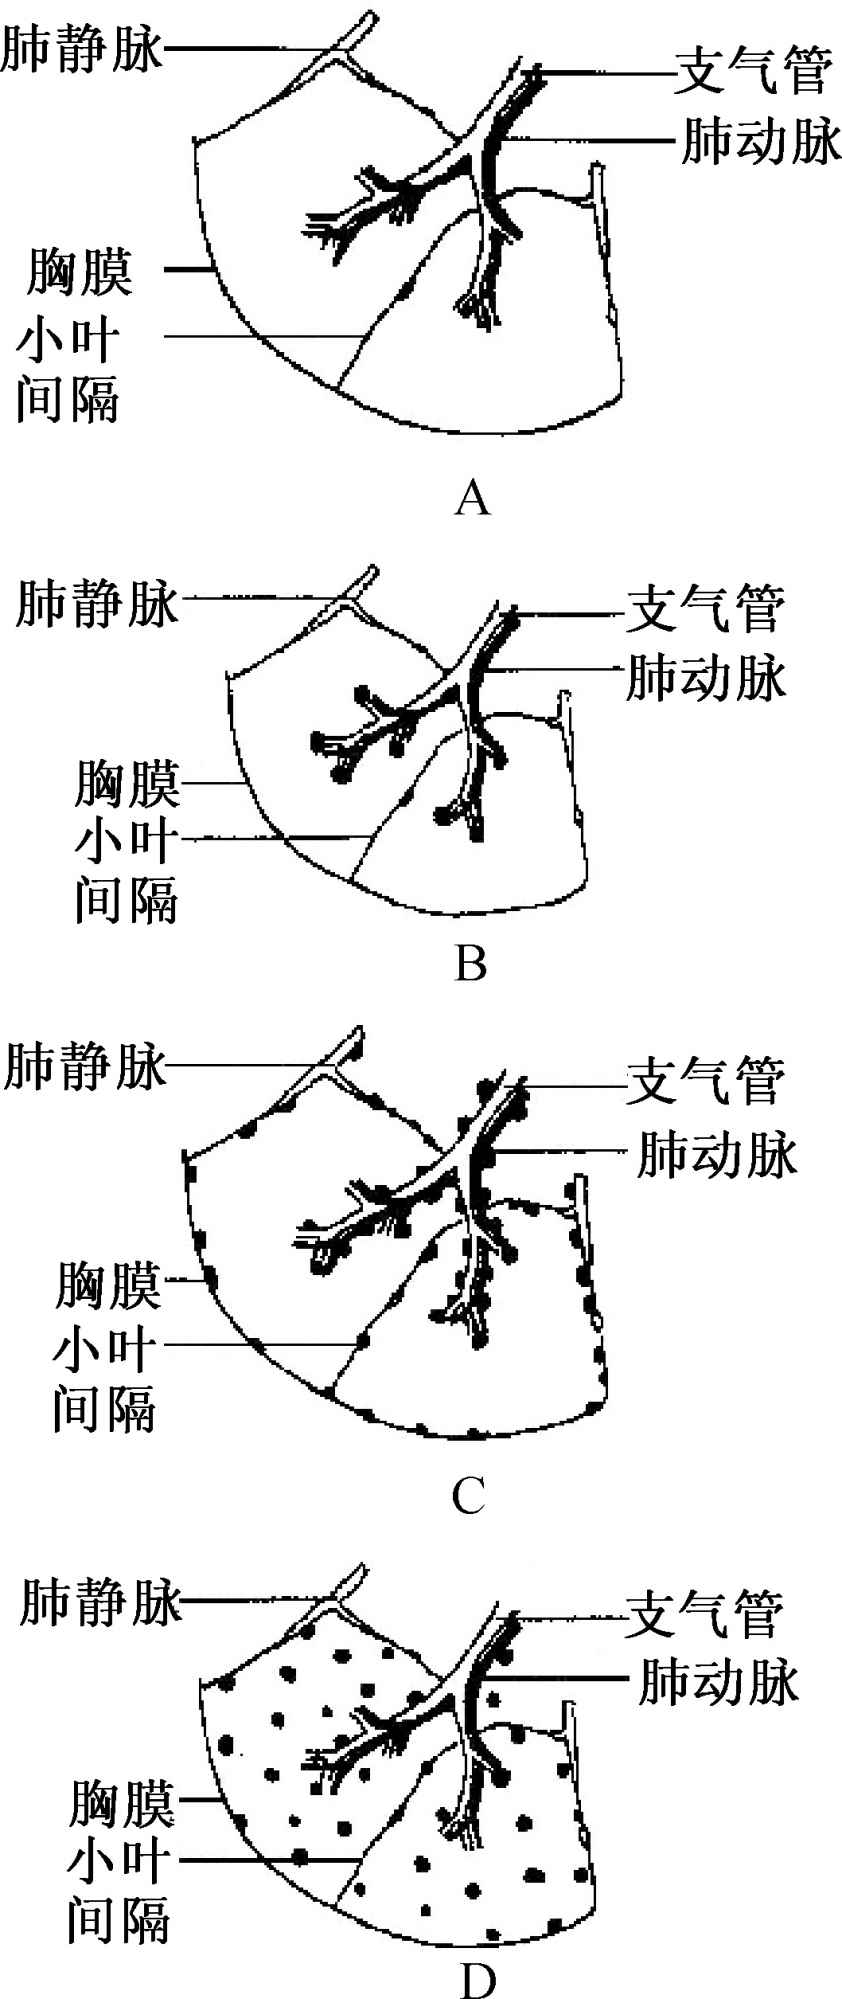
\includegraphics[width=.7\textwidth,height=\textheight,keepaspectratio]{./images/Image00186.jpg}
 \captionsetup{justification=centering}
 \caption{肺内弥漫性多发小结节的HRCT示意图\\{\small A.正常肺小叶结构;B.小叶中心分布结节;C.淋巴管周围分布结节;D.随机分布结节}}
 \label{fig9-3}
  \end{figure} 

1.小叶中心结节:位于小叶中心,结节不与小叶间隔及胸膜相连,与两者间隔5~10mm。肺脏中、内区的支气管血管束周围也无分布。主要见于过敏性肺炎、嗜酸性肉芽肿、尘肺以及闭塞性细支气管炎(BO)、闭塞性细支气管炎并机化性肺炎(BOOP)。

2.小气道结节:亦位于小叶中心,但主要表现为“树枝发芽”征。此征见于多种炎性疾病:①经支气管播散的感染:如支气管播散性结核、支气管肺炎的早期、吸入性肺炎;②小气道疾病合并感染:如弥漫性全支气管炎、感染性细支气管炎;③气道疾病合并小分支的黏液栓塞:如过敏性支气管肺曲菌病等。

3.淋巴管周围结节:为淋巴管病变所致,主要分布在淋巴管内及周围。淋巴管位于支气管血管束、小叶间隔及胸膜。故此型结节主要沿支气管血管束、小叶间隔和胸膜下分布,也可位于小叶中心。见于癌性淋巴管炎、结节病、尘肺等。

4.随机分布结节:是经血行播散至肺内,又称为血源性结节。结节的分布与肺小叶的各个结构无特殊关系,在分布上呈随机性。结节广泛分布于肺的各个部位,既可位于肺间质,亦可见于小叶中心或小叶中心与小叶边缘间的肺组织。见于血源性肺转移癌、急性粟粒型肺结核和血源性真菌病等。

此外,鉴别时应注意:①胸膜下结节见于淋巴管周围结节及血源性结节;②胸膜下无结节见于小叶中心分布的结节;③小叶中心结节多边缘模糊;间质结节及气道疾病结节边缘清晰;④小叶中心结节不具有“树枝发芽”征者主要见于过敏性肺炎、嗜酸性肉芽肿和尘肺等。

\subsection{常见的几种弥漫性肺疾病支气管血管束异常HRCT特点}

1.支气管血管束增粗及边缘毛糙不规则、扭曲变形者:主要见于慢性支气管炎合并间质纤维化、结缔组织疾病纤维化。其病理改变包括支气管血管周围间质及其肺实质炎症、纤维化。

2.支气管血管束增粗且呈结节状或串珠状征象者:见于结节病、癌性淋巴管炎、淋巴瘤、煤工尘肺等。结节病的病理基础是非干酪样肉芽组织结节沿支气管血管周围淋巴管分布,可伴或不伴间质纤维化;癌性淋巴管炎为支气管血管束周围淋巴管内的肿瘤细胞生长。

3.小叶中央支气管血管束异常、表现为小叶核影增大者:见于煤工尘肺、癌性淋巴管炎、慢性支气管炎等。在煤工尘肺为小叶内支气管血管周围尘肺结节所致;在癌性淋巴管炎为小叶内以血管为中心的癌结节所致;慢性支气管炎则是细支气管周围炎性病变所致。

4.小叶核分支状影增多者:见于毛细支气管炎、支气管播散性肺结核、支气管扩张等。病理表现为小叶内细支气管扩张,并见管壁及周围肺组织炎症细胞浸润。

\subsection{肺门肿块}

\subsubsection{病因}

常见的有:①淋巴结增大:多见于结核、结节病、尘肺、转移瘤、恶性淋巴瘤、巨淋巴结增生症等;②肿瘤:多为中心型肺癌,少数为腺瘤;③血管性病变:动脉瘤、静脉瘤及其他血管扩张性改变。

\subsubsection{CT表现}

①部位:淋巴结增大位于支气管分叉部;支气管肿瘤位于支气管旁和周围;血管性肿块与肺动、静脉相连。②形态:淋巴结增大呈圆形或分叶状;支气管肺癌呈球形、长圆形或不规则状;血管性肿块多为圆形。③密度:多为软组织密度,但可钙化,如结核钙化为斑片状或斑点状;尘肺为斑点状、蛋壳状或完全钙化;少数中心型肺癌也可有斑点或斑片状钙化。④增强扫描:血管性肿块可明显强化,可合并血管栓塞;巨淋巴结增生症多显著强化。⑤在分析肺门肿块时还应注意支气管、肺内及纵隔的异常等。

\subsection{胸膜病变}

主要有以下基本CT表现:①游离性胸腔积液;②局限性胸腔积液:包括包裹性胸腔积液、叶间积液、肺下积液和纵隔胸膜腔积液;③气胸和液气胸;④胸膜增厚和粘连;⑤胸膜钙化;⑥胸膜结节及肿块。

CT有助于少量积液的显示。HRCT有助于轻度胸膜增厚(1mm左右)的诊断,可呈线形高密度影,并可见增厚胸膜与胸壁之间1~4mm的胸膜外脂肪。光滑的增厚见于脓胸或慢性胸膜炎性病变。单发的胸膜肿块为胸膜纤维瘤、局限分布的恶性胸膜间皮瘤、畸胎瘤及转移瘤等,结核亦可有此表现。多发、弥漫性胸膜结节多见于胸膜转移瘤及间皮瘤。

\subsection{纵隔病变}

\subsubsection{纵隔移位、纵隔疝}

如两侧胸腔压力失去平衡则纵隔发生移动,其原因如下:

1.向健侧移位:由于病变推压纵隔所致,如胸腔积液、气胸、较大的肺肿瘤、一侧肺气肿、一侧横膈升高、膈疝及横膈破裂等。

2.向患侧移位:由于病变牵拉纵隔所致,如肺广泛纤维化、胸膜肥厚、肺不张、肺叶或全肺切除等。

3.脊柱畸形:脊柱侧突畸形或肋骨发育异常亦可引起纵隔位置、形态的改变。

纵隔疝是由于一侧胸腔压力明显高于对侧时,除纵隔向对侧移位外,还伴有部分肺组织和纵隔胸膜通过纵隔的生理薄弱点疝入对侧胸腔。疝入的部位多在前上及后下纵隔的薄弱区。纵隔疝可见于大量胸腔积液、张力性气胸、巨大肺大泡及肺切除术后代偿性肺气肿等。

\subsubsection{纵隔的病理形态改变}

1.纵隔增宽:①局限性向一侧或两侧突出:多见于纵隔肿瘤,肿块的形状、位置、大小、边缘因肿瘤性质不同而异。②向两侧普遍增宽:多见于纵隔急性或慢性炎症,边缘模糊。急性者其内可见脓腔及液平面等表现。

2.纵隔变窄:多见于两肺慢性弥漫性肺气肿。

\subsubsection{纵隔气肿}

气体积聚于纵隔内称为纵隔气肿。

\subsection{膈病变}

1.形态异常:①胸膜增厚粘连时可见膈的边缘失去光滑的形态,并有条状高密度影像,多见于结核和慢性炎症;②膈的局限性肿块呈球形或扁丘状隆起,见于平滑肌瘤、脂肪瘤、血管瘤、纤维瘤、囊肿、包虫囊肿、转移瘤等;③膈疝可见膈肌失去连续性。

2.位置异常:①两膈位置下降:见于肺气肿、两侧横膈强直性痉挛等;②单侧膈位置下降:一侧肺气肿、大量胸腔积液、大量气胸等;③两侧膈升高:见于腹水、肺间质纤维化、妊娠、腹腔巨大肿瘤、肠管大量胀气、两侧膈胸膜肥厚粘连;④单侧膈升高:胸内原因有先天性无肺或发育不全、肺不张、一侧胸膜肥厚粘连;腹内原因有膈下脓肿、肝脓肿、肝脾增大、肝脾肿瘤、巨大肾肿瘤、肾积水、肾上腺肿瘤、胃泡或结肠脾区充气;膈本身的原因有膈麻痹、膈膨升、膈疝。

\section{气管支气管疾病}

\subsection{气管性支气管}

正常情况下,气管分为左、右主支气管。如从气管直接分出一个异位的支气管或一个额外的支气管到肺叶或肺段称为气管性支气管。这一畸形很少见,且都发生于右侧。一般气管性支气管开口离气管隆突较近。

临床无任何症状。常规X线难以显示,而支气管造影和CT可以发现。

\subsection{先天性气管狭窄}

\textbf{【病因病理】}
本病是气管先天性发育异常或胚胎期前肠分隔气管与食管时发生障碍引起气管狭窄。根据病变范围及病因可分为两种:①局限性:主要为纤维性狭窄,气管腔内有环形或新月形隔膜;②弥漫性:累及气管全长,主要由气管软骨环发育不全所致。

\textbf{【临床表现】}
多无临床症状,可有喘憋、呼吸困难及上呼吸道反复感染。

\textbf{【CT表现】}
气管内腔横断面各个径线变小。气管软骨的异常有软骨环缺如。纤维性狭窄病变范围短,呈漏斗状;而气管软骨环发育不全范围广。

\textbf{【鉴别诊断】}
①外伤、手术或导管长期滞留所致的气管狭窄表现为有肉芽组织和息肉形成的软组织影像,结合病史不难鉴别。②应注意与外压性狭窄和气管肿瘤及复发性多软骨炎等鉴别。

\subsection{先天性气管软化症}

本病为气管壁的异常软弱,可累及主支气管,故又称气管、支气管软化症。

\textbf{【病因病理】}
气管软骨环发育不全时,气管壁的支持力不足,造成呼气期气管变形或完全萎缩。呼气时表现为气管冠状径缩小。

\textbf{【临床表现】}
可以是非特异性的喘鸣、喘息和咳嗽。过度的伸颈呼吸和反射性的呼吸暂停常提示本病。气管内分泌物引流不畅可致上呼吸道反复感染。

\textbf{【CT表现】}
气管冠状径狭窄、矢状径正常。一般冠状径小于矢状径的50%即可诊断本病。狭窄的气管内壁光滑,管壁无增厚,也无钙化。深吸气末或尽力呼气后屏气扫描,管腔可有变化。

\textbf{【鉴别诊断】}
①刀鞘样气管:病因不明,可能为反复咳嗽后造成的气管软骨的退行性变。特征为胸内气管冠状径缩小、矢状径正常,但其管壁可见钙化、不同呼吸时相管腔的形态无改变(结合透视动态观察很有价值)。②需注意结合病史与长期插管气管壁损伤所致的局限性软化鉴别。此外,多软骨炎、周围肿块的压迫、邻近血管压迫、食管气管瘘,也可导致气管软化;我们还曾见1例长期应用肾上腺皮质激素所致者,应注意结合病史鉴别。

\subsection{巨气管支气管症}

本病又称为Mounier-kuhn 综合征。

\textbf{【病因病理】}
是因气管和主支气管平滑肌和弹力纤维发育不良而引起的管腔明显扩张。病理上因气管和支气管壁异常无力,导致尽力呼气和咳嗽障碍,阻碍正常的纤毛运动,且因为反复感染,最终导致支气管扩张。

\textbf{【临床表现】}
多为30~40岁男性。可伴有反复的肺部感染。也有少数无明显症状。普通X线检查可见气管主支气管吸气时扩张,而呼气时可有萎缩(与单纯呼气时才有的气管狭窄或萎缩,而无明显扩张的气管软化症不同)。

\textbf{【CT表现】}
气管和支气管内径增大:可达30~50mm,最宽达50~60mm,主支气管内径可达25~35mm;叶和叶以下支气管多正常,但亦可扩张。气管内壁光滑,在软骨环间向外突出,但CT不易发现。肺内可有斑片状炎症。总之,当气管横径、前后径男性超过25mm、27mm或左、右主支气管径超过18mm、21mm;而女性则分别超过21mm、23mm和17.4mm、19.8mm即可诊断。

\textbf{【鉴别诊断】}
应注意与以下疾病相鉴别:①结节病和囊性纤维化等导致的严重肺上叶纤维化可牵拉气管、支气管导致其扩张;②慢性气道感染如吸烟、慢支、肺气肿和囊性肺纤维化可引起气管支气管软化,亦可表现为弥漫性气道扩张和软化;③气道感染性疾病如过敏性支气管肺曲菌病亦可引起中央气道或中央性支气管扩张。

\subsection{气管憩室}

气管憩室是先天性气管壁的局部缺陷所致的罕见病。

\textbf{【病理】}
一般见于气管的后壁即气管软骨环的缺口处或气管的膜部。憩室常有较窄的颈部,而有人将基底部较宽者称为囊样膨出。一般多偏于右侧,因气管左壁与食管紧邻,故左侧少见。单个的憩室也可能为原始异位支气管芽的遗留。多发的憩室可伴有巨气管支气管、气管壁内肌肉和弹力纤维发育不全。

\textbf{【临床表现】} 气管憩室本身无症状,而偶然发现。

\textbf{【CT表现】}
气管旁(多为右侧)低密度含气腔,边缘光滑,以狭颈或广口与气管相通。其内偶可见液气平面影。邻近血管可受压移位。

\textbf{【鉴别诊断】}
①支气管含气囊肿继发感染:系支气管囊肿继发感染后与气管支气管发生交通,但常有继发感染的临床及CT表现,可予区别。②颈部气管重复畸形:系喉气管沟先天性发育异常所致,可形成颈部包块。CT见颈部气管旁一含气囊腔影,无直接交通口。但手术可见含气腔结构与气管壁相连。

\subsection{先天性支气管闭锁}

\textbf{【病因病理】}
本病为胚胎发育过程中节段性的支气管从索状演变为管道受障所致。好发于两肺上叶尖后段支气管开口处,尤以左侧多见,也可位于肺叶或肺亚段支气管。闭锁远端的支气管因黏液潴留而发生扩张,相应肺组织发育正常,由侧支通气而含气。

\textbf{【临床表现】}
约1/3患者有气短、咳嗽等症状。胸片有分支状肿块影像。

\textbf{【CT表现】}
①局限性阻塞性肺气肿:吸气期气体由侧支通气而通气,而呼气期不能顺利排出最终导致肺气肿。②支气管黏液栓塞:黏液栓塞的支气管与CT扫描层面平行时呈“V”形、“Y”形或多个分支条状、手指状影像;支气管与扫描层面垂直时呈结节状影像。其CT值为-5~20Hu,黏液浓缩后为30~50Hu。这时远端肺组织密度可减低。③黏液囊肿:呈圆形,边缘光滑,密度同上。

\textbf{【鉴别诊断】} 需注意与气管内肿瘤、过敏性支气管肺曲菌病鉴别。

\subsection{先天性支气管囊肿}

先天性支气管囊肿可发生于肺和纵隔(纵隔支气管囊肿见本章第二十节),发生于肺内者称为肺囊肿。

\textbf{【病因病理】}
肺芽从胚胎的原始前肠发生。从胚胎第六周起,两侧肺芽开始分叶,右侧三叶,左侧两叶。支气管发育是从索状组织演变成中空的管状组织。期间如发育停止,不能使索状结构成为贯通的管状结构,远端支气管分泌物不能排出,可积聚膨胀形成囊肿。如仅涉及一个支气管芽则形成孤立性囊肿;如不发育的索状部分已分支,涉及多个支气管芽,则形成多发性囊肿;如有局部小块组织从整个组织上脱落,则形成与支气管毫无联系的囊肿(此种情况多见于纵隔)。多发性支气管囊肿可合并支气管肺发育不良。本病一般下叶比上叶多,左肺多于右肺。囊肿壁较薄,有呼吸上皮、软骨、平滑肌和黏液腺体等结构。

\textbf{【临床表现】}
新生儿期一般无症状,仅有少数有呼吸困难。较大儿童和青年可出现反复感染症状如发热、咳痰、咯血和喘鸣,也可无症状。肺囊肿易反复感染。

\textbf{【CT表现】}

1.孤立性肺囊肿:有3种表现形式:①含液囊肿:呈圆形或椭圆形高密度灶,密度均匀、边缘光滑锐利。液体一般较稠厚、含有较多胶冻样蛋白质成分,故密度较一般囊肿高,CT值约20~30Hu。②含气囊肿:如囊肿与支气管相通,液体排出代之以空气而形成含气囊肿;或因支气管发育畸形而使肺内中、远端支气管形成活瓣性阻塞,气体易进难出而形成单纯含气囊肿。囊壁菲薄,约1mm左右,多<2mm。有时有间隔,呈多房性。③液气囊肿:囊肿与支气管相通仍含有部分液体而形成液气囊肿;或因含气囊肿继发感染所致。后者囊肿壁可增厚,周围可有斑片状渗出灶。

2.多发性肺囊肿:多为含气囊肿,可分布于一叶或多叶、一侧或两侧。呈弥漫性多发薄壁环形透亮影,边缘锐利,部分囊肿内可有浅小液平(图\ref{fig9-4})。气囊大小不等,自豌豆至桃子大小,密集者形如蜂窝。有时呈串珠状高密度灶。可合并支气管肺发育不良,表现肺体积缩小,常伴胸膜增厚。

\begin{figure}[!htbp]
 \centering
 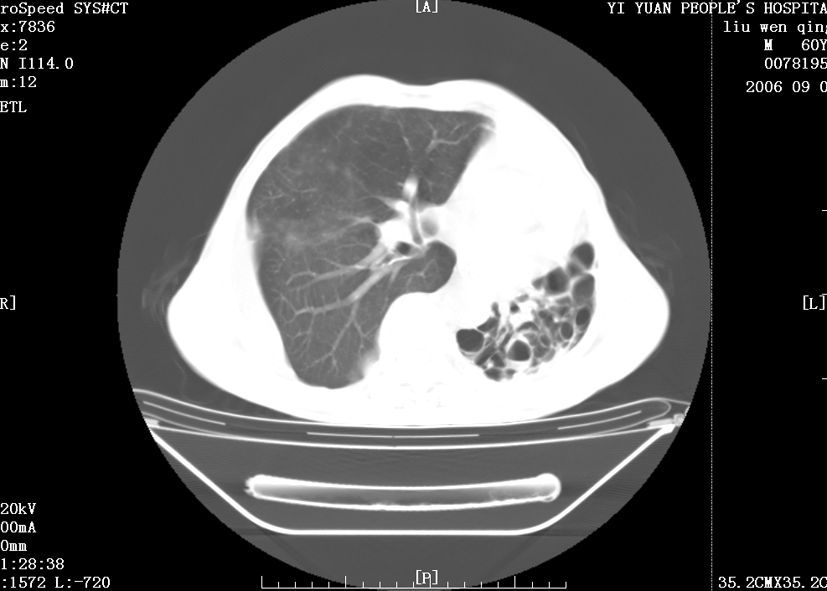
\includegraphics[width=.7\textwidth,height=\textheight,keepaspectratio]{./images/Image00187.jpg}
 \captionsetup{justification=centering}
 \caption{多发性肺囊肿\\{\small 左肺弥漫性分布有无数薄壁环形透亮影,部分囊肿内有浅小液平,并左肺发育不良致气管纵隔显著左移位}}
 \label{fig9-4}
  \end{figure} 

有人将肺囊肿分为薄壁囊腔型、厚壁囊腔型(壁厚\textgreater{}2mm)和肿块样型。厚壁型与反复感染有关;肿块样型与囊内出血、含高蛋白液体或含钙乳样物质,以及囊壁大量纤维组织增生、肉芽肿形成或合并炎性假瘤形成有关。

3.其他表现:①增强扫描:囊壁轻、中度强化,尤其含液囊肿易显示,如继发感染强化较明显。②含气囊肿可继发曲菌球,呈囊肿内球环形软组织影。③囊壁可有钙化(软骨钙化及反复感染、出血所致),呈点状或弧形,以弧形最具特征性。④囊肿周围可有局限性肺气肿,在肺内孤立性球形病灶中,其他疾病很少有此表现。⑤可合并其他先天性疾病如肺隔离症、先天性膈疝等。⑥肺囊肿偶可破裂形成气胸。

4.肺囊肿并发感染:若肺囊肿继发感染,则在其周围出现浸润性炎症病灶,邻近胸膜可增厚;也可感染时囊肿增大,感染控制后缩小。囊壁增厚多>2mm。囊肿与周围组织粘连使其形态不规则、边缘模糊。有时边缘有分叶征、毛刺征,尤其肿块样型与肺癌可难以鉴别。增强扫描可提供一定的鉴别诊断依据。

有时肺囊肿继发感染后,囊内有干涸脓液、肉芽组织及少量气体,而在囊内形成半月形的低密度空气区,称为空气半月征。

5.恶变表现:先天性肺囊肿有少数可发生恶变,显示含气囊肿的囊壁内缘有不规则软组织结节生长,或含液囊肿迅速增大、边缘不规则。

\textbf{【鉴别诊断】}

1.肺脓肿:先天性肺囊肿继发感染后,囊肿周围有炎症浸润、囊肿内可有少量液平,类似肺脓肿。其区别为:①先天性肺囊肿周围的炎性浸润比肺脓肿少;②囊内液体与腔外浸润不成比例;③囊壁相对比脓肿壁薄;④急性肺脓肿治疗后可完全消失;⑤慢性肺脓肿往往有较广泛的纤维化,而囊肿反复感染见纤维化局限于囊壁周围。此外,先天性肺囊肿继发感染后往往能找到一段比较规整且薄的囊壁,这点有鉴别意义。

2.后天性肺气囊肿:①气肿性大泡:伴有周围组织的气肿征象;②感染后肺气囊肿常有肺部化脓感染史,但残留的感染后肺气囊周围肺野可无任何异常改变。

3.肺隔离症:亦可呈囊状表现,但常位于下叶后基底段,以左侧多见。结合其异常的主动脉供血血管影多能鉴别。

4.先天性囊腺瘤样畸形:为细支气管和肺泡的发育畸形所致。呈多发的囊状或囊实性改变,病灶较大且有明显的占位征象,纵隔向健侧移位有助于鉴别。但也可呈单发的薄壁囊肿,且无血供异常,与肺囊肿难以鉴别。

5.肺包虫囊肿:呈水样密度且边缘光滑的囊性肿块,可与支气管相通而含液气平面。囊壁钙化以及内囊分离为其典型表现。结合疫区居住史和血清试验可资鉴别。

\subsection{气管支气管骨软骨形成症}

本病又称骨化性气管支气管病、骨软骨发育不良性气管病。是指在气管、支气管内有结节性骨、软骨增生。

\textbf{【病因病理】}
本病的发生可能与慢性炎症、退行性变、化学或机械刺激、代谢异常、先天性素质等有关。病理主要表现为小结节内可见软骨灶和骨化灶。

\textbf{【临床表现】}
多见于50岁以上,男性多于女性。通常无症状,可有呼吸困难、干咳、咳痰、咯血等症状。

\textbf{【CT表现】}
早期可见气管软骨环处(一般不累及气管的后部膜性部分)向管腔内突出的小结节状影像,CT值较高,部分钙化为骨性密度。大小1~7mm不等,多为2~4mm。一般黏膜下高密度钙化影与气管环不连接。可累及叶支气管。病变严重者可有气管支气管壁增厚、气管环钙化、多发性骨化及软骨结节、长段管腔狭窄。

\textbf{【鉴别诊断】}
多发黏膜下高密度钙化小结节并突向管腔内是气管支气管骨软骨形成症的较特征性表现。而且由于多不累及气管的后部膜性部分而与复发性多发性软骨炎、气管淀粉样变(也可有管壁钙化)不同。

\subsection{复发性多发性软骨炎}

本病主要累及全身软骨组织和含有多量黏多糖类的组织。

\textbf{【病因病理】}
病因尚不明,可能与粘多糖代谢异常及自身免疫性血管炎(属结缔组织疾病)有关。病理改变为软骨破坏和结缔组织增生。

\textbf{【临床表现】}
以40岁左右多见,男女发病率相近。两个或两个以上部位的软骨反复发生炎症。气道受累约占半数,有咳嗽和呼吸困难。喉、耳、鼻软骨受累可有相应表现。总之,其主要特点为多关节炎、动脉炎、葡萄膜炎和复发性软骨炎,反复肺部感染是病人发病和死亡的主要原因。

\textbf{【CT表现】}
①较广泛的、长段的气管、主支气管狭窄和腔壁增厚、钙化,还可累及中间段和上、下叶支气管。②杓状软骨和环状软骨肿胀、密度增高及钙化。③肺内常合并肺炎和肺气肿改变。

\textbf{【鉴别诊断】}
弥漫性中央气道狭窄除复发性软骨炎外,主要还有溃疡性结肠炎、淀粉样变、结节病、韦格纳肉芽肿、气管支气管骨软骨形成症和各种感染,并均可有气管壁增厚、狭窄和钙化。恶性肿瘤偶可引起弥漫性中央气道狭窄。军刀鞘状气管与弥漫性气管狭窄表现相似,是慢性阻塞性肺疾病的表现,亦可有轻度支气管壁增厚伴气管环的钙化。

\subsection{细支气管炎的分型}

本病综合有关文献可将分为5型:①闭塞性细支气管炎(BO):又称为缩窄性细支气管炎;②闭塞性细支气管炎并机化性肺炎(BOOP):又称为增生性细支气管炎;③细胞性细支气管炎;④全细支气管炎:又称为弥漫性全细支气管炎;⑤呼吸性细支气管炎(RB)及呼吸性细支气管炎-间质性肺病(RB-ILD)。

上述5类细支气管炎的影像学改变是非特异性的,应密切结合临床,且多需活检确诊。

\subsection{闭塞性细支气管炎(BO)}

本病亦称为缩窄性细支气管炎、细支气管炎闭塞综合征。其病理定义是导致气道腔变窄或阻塞的小气道壁的不可塑性纤维化。

\textbf{【病因病理】}
与感染、免疫等因素有关,特发少见。其主要病因有儿童时期的病毒、支原体、麻疹等感染,有毒气体、化学物质、刺激性气体的吸入,结缔组织病,器官或骨髓移植及药物(青霉素、可卡因)反应等。此外,中年妇女可出现原因不明的BO。其病理特点是细支气管壁瘢痕引起的向心性狭窄、平滑肌细胞增生肥大以及黏液栓塞。

\textbf{【临床表现】}
严重的进行性气道阻塞而致呼吸困难。尽管类固醇治疗可阻止病程发展,但肺功能很少随之改善,因为小气道的瘢痕是不可逆的。继发于小气道感染(主要为腺病毒)的BO可导致Swyer-James综合征,典型者在8岁前即肺泡尚没有完全发育时发病,这个特殊的综合征仅指儿童,其典型影像学表现为:肺野透光度高、肺容量减少,同侧肺门变小,外周血流减少,以及出现空气滞留征。

\textbf{【HRCT表现】}
①直接征象:惟一的征象为细支气管壁增厚,呈小叶中心的分支样影和小叶中心结节。②间接征象:常见的有支气管细支气管扩张、肺密度的马赛克表现及呼气性空气滞留。

\subsection{闭塞性细支气管炎伴机化性肺炎(BOOP)}

本病亦称为增生性细支气管炎、闭塞性细支气管炎伴腔内息肉、特发性机化性肺炎。其病理定义是指小气道被息肉样肉芽组织填塞(闭塞性细支气管炎)以及蔓延到气道远端肺泡的扩散过程(机化性肺炎)。BOOP曾经与BO相混淆,1985年英国学者将其作为一种临床病理学类型从BO中独立出来。

\textbf{【病因病理】}
本病特发多见,亦可与感染有关。一些特发性病例与结缔组织疾病、自身免疫性疾病、药物反应以及骨髓和肺移植等相关。其病理改变为细支气管、肺泡管、肺泡囊内成纤维细胞导致的不完全纤维化或颗粒状息肉形成,在细支气管肺泡周围出现巨噬细胞、单核细胞浸润,其管腔内有局限性纤维化。

\textbf{【临床表现】}
平均发病年龄55岁。多呈亚急性,病程短,症状可持续2~6个月(平均小于3个月)。表现为咳嗽、咳痰、呼吸困难、发热、不适以及体重下降。与BO的区别是:BOOP为亚急性病,而不像BO为慢性病;肺功能试验是限制性的,而不像BO以阻塞性改变为主,而且BOOP类固醇治疗有效。

\textbf{【HRCT表现】}
更常累及下肺区,典型表现为:①片状实变或磨玻璃影,通常为胸膜下或支气管旁分布;②小叶中心结节;③肺病变区内支气管壁增厚或扩张;④碎路石征(即磨玻璃影伴小叶间隔增厚)亦常见;⑤还可见不规则线状影及胸膜下轻度的蜂窝影、胸膜渗出。以①最常见。

\subsection{细胞性细支气管炎}

本病又称感染性细支气管炎。本病是指支气管壁和腔内急性、活动性炎症的过程。

\textbf{【病因病理】}
急性感染性细支气管炎是其原因之一,包括病毒、支原体、流感嗜血杆菌、结核、曲霉菌感染等,以炎性细胞浸润为特征。在婴儿呼吸道合胞病毒感染亦是常见原因。其他与哮喘、吸入性肺炎、慢性细支气管炎和过敏性肺炎有关。病理可见上皮细胞脱落坏死、管腔内充满炎性渗出物及脱落的上皮细胞,使管腔部分或完全阻塞。成年人的感染性细支气管炎是可逆的。

\textbf{【临床表现】}
急性感染性细支气管炎常见于婴幼儿。临床以发热、气短、喘息、过度充气为主。

\textbf{【HRCT表现】}
①外周小叶中心的线状或结节状阴影即所谓的“树芽征”。②另一表现是小而边界不清晰的小叶中心结节,均匀、弥漫分布,高度提示高敏感性肺炎。③还常见非特异性斑片状、磨玻璃状高密度灶,说明可能伴随感染引起的支气管肺炎。④间接征象有空气潴留、亚段肺不张。

\subsection{全细支气管炎}

本病又称为弥漫性全细支气管炎,是原因不明的慢性炎症。在北美和欧洲少见,是亚洲人种的一种特发感染的肺部疾病,尤其多见于日本男性。

\textbf{【病理】}
为呼吸性细支气管的单核细胞炎症。其特征包括细支气管的淋巴细胞渗出引起管壁增厚,支气管扩张引起的分泌物和泡沫样巨噬细胞填充于有慢性炎症的气道和与之相邻的肺泡。炎症范围从小叶中央的气道到相邻的间质,不累及气腔。后期可出现细支气管腔狭窄,伴有病变部位近端细支气管扩张。

\textbf{【临床表现】}
由于呼吸道的反复感染,多表现为非特异性进行性呼吸困难、咳嗽、咳痰、肺功能损害。大多抗生素(红霉素)治疗有效,但长期预后仍较差。

\textbf{【HRCT表现】}
结节样表现和小气道分支不透光影主要沿小叶中央分布即树芽征,是小气道嵌塞所致。常伴轻度柱状支气管扩张,少数可见马赛克表现。可发展为闭塞性支气管炎(BO),且可继续进展为BOOP。

\subsection{呼吸性细支气管炎及呼吸性细支气管炎-间质性肺病}

\subsubsection{}

本病又称为“吸烟者”的细支气管炎,是大多数吸烟者肺组织学的表现。

\textbf{【病理】}
其特征为呼吸性细支气管轻度慢性炎症和呼吸性细支气管及相邻肺泡内巨噬细胞及色素聚集,伴有细支气管周围轻度纤维化。

\textbf{【临床表现】}
很少有临床症状和胸片的异常表现,肺功能检测轻度受限、通气量减少。

\textbf{【HRCT表现】}
仅少数有异常表现,最常见的是散在分布的磨玻璃样及小叶中心的微小结节密度灶。同时上叶区域常见肺气肿。

\subsubsection{}

本病是指有症状的呼吸性细支气管炎,该类病人有大量吸烟或长期接触烟草史。其病理和影像学类似于间质性肺炎的改变,故称为RB-ILD。

\textbf{【病理】}
其特征为呼吸性细支气管及相邻肺泡内巨噬细胞及色素聚集,同时伴有中度细支气管周围的间质纤维化增厚。尽管组织学与RB相似,但RB-ILD有大范围的肺实质组织受累。

\textbf{【临床表现】}
常常表现为慢性咳嗽、呼吸困难和限制性肺功能障碍。停止吸烟后症状改善。

\textbf{【HRCT表现】}
常表现为磨玻璃样密度影或小叶中心结节、支气管壁增厚、线状或网状小叶间隔增厚、肺气肿、肺膨胀不全。亦有学者发现与脱屑性间质性肺炎的病变相似。有的亦可无明显异常。

\subsection{支气管哮喘}

哮喘是非特异性炎症,大小气道均可受累。

\textbf{【病理】}
其病理学改变是多细胞参与的,其炎细胞与炎性介质均处于活动状态而组成复杂的细胞网,可减轻炎症,但同时可导致气道重塑,从而使大小气道内腔发生改变。哮喘病人的炎性反应主要出现在外围的中央气道。有研究发现在大小气道同时出现T细胞、嗜伊红细胞的聚集,同时活动性嗜伊红细胞出现在小气道的数量多于大气道。哮喘引起的气体交换异常,部分原因在于小气道。其他病理改变包括上皮受损、倒伏、气道壁纤维化、平滑肌细胞肥大及血管扩张等均可导致气道壁增厚。

\textbf{【临床表现】}
①外源性哮喘:即过敏性哮喘。多有明显季节性,发作前有致敏源接触史。可分为前驱期、发作期和缓解期。发作期以发作性、呼气性呼吸困难为突出症状,两肺满布哮鸣音,以呼气末更明显。②内源性哮喘:多指感染性哮喘而言。其发作期较长,当感染控制后哮喘可缓解,但不易彻底。内源性哮喘还包括药源性、职业性、神经精神性、运动性等。

\textbf{【HRCT表现】}
其表现是多样的。常仅有很轻微的变化,也可有气管壁增厚、支气管扩张、小叶中心结节、气肿、马赛克样灌注和气体潴留。其中特征性表现为细支气管壁的显著增厚。气管壁的增厚与哮喘的严重程度相关。

\subsection{慢性支气管炎}

本病是指气管、支气管黏膜及其周围组织的慢性非特异性炎症。支气管内长期产生多量黏液分泌是其主要症侯。

\textbf{【病理】}
支气管黏液腺体增生、腺管增宽,支气管内分泌物增多、黏稠,常堵塞小支气管。支气管黏膜充血、水肿、上皮细胞萎缩、鳞状上皮化生。支气管管壁弹性纤维破坏及增生。支气管周围慢性炎症及纤维化。可合并肺内炎症、肺气肿、肺间质纤维化和肺心病。

\textbf{【临床表现】}
咳嗽、咳痰,严重时有发热、喘憋和呼吸困难。临床诊断标准为慢性进行性咳嗽2年以上,每年至少3个月;或一年连续咳嗽3个月以上。临床诊断必须排除其他肺部疾病。

\textbf{【CT表现】}
一般采用常规CT扫描,对于肺间质纤维化者应薄层CT或HRCT扫描。本病早期并无异常或特异性表现。

后期主要CT表现为(图\ref{fig9-5}):

\begin{figure}[!htbp]
 \centering
 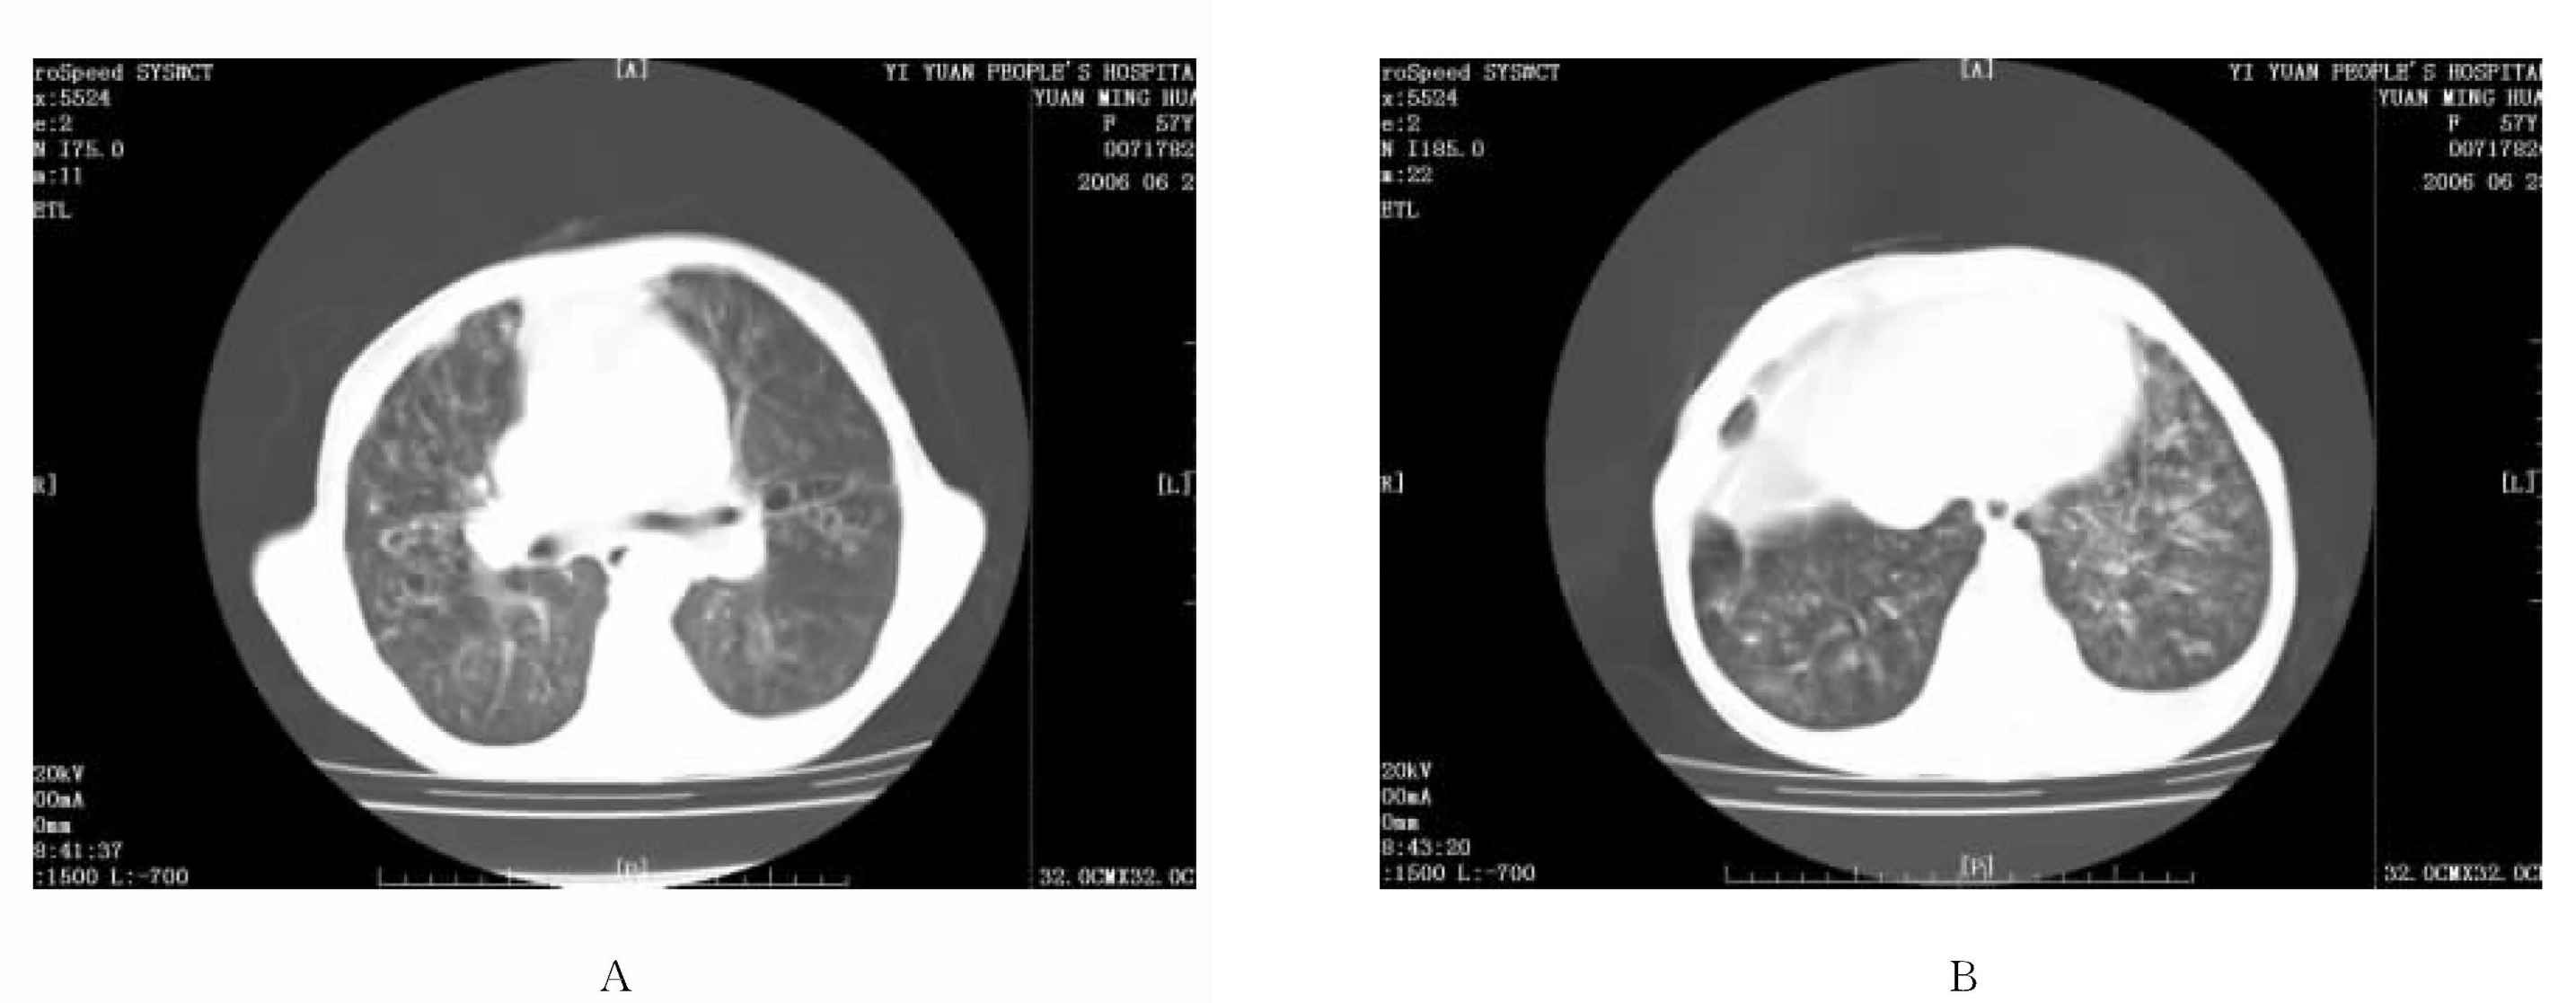
\includegraphics[width=.7\textwidth,height=\textheight,keepaspectratio]{./images/Image00188.jpg}
 \captionsetup{justification=centering}
 \caption{慢性支气管炎\\{\small 合并支扩、感染、肺间质纤维化}}
 \label{fig9-5}
  \end{figure} 

1.支气管壁增厚:以两下肺多见,形成轨道征或称为双轨征。可合并支气管扩张。

2.肺气肿:胸廓增大,膈肌低平。①小叶中心型肺气肿:呈多发的近圆形无壁低密度区;②全小叶型肺气肿:呈较广泛的低密度区,可伴血管支气管变细;③间隔旁肺气肿:为位于胸膜下的、多<1cm的低密度区。有学者认为10mm层厚扫描CT值<-910Hu,1mm层厚扫描CT值<-950Hu可诊断为肺气肿。

3.肺大泡:为局限的无肺组织结构的区域,常位于胸膜下,壁薄、周围肺组织受压。可合并感染出现液平面。

4.肺内炎症:为斑片状影像,两下肺多见。

5.肺间质纤维化:小叶间隔增厚、小叶内间质增厚,晚期可有蜂窝肺及牵拉性支扩。

6.肺动脉高压及肺心病:肺门区肺动脉增粗,右下肺动脉干宽>15mm。肺心病时右心室增大。

\textbf{【鉴别诊断】}
本病所引起的肺间质纤维化与特发性肺间质纤维化CT表现相似,但慢支常引起肺气肿改变,且有显著的胸廓增大和膈位置下降。

\subsection{支气管扩张症}

本病是指1支或1支以上支气管不可逆性增宽的慢性疾病。

\textbf{【病因】} 分为以下两类:

1.先天性:包括①纤毛无运动综合征:为常染色体遗传性疾病,由于呼吸道纤毛和精子尾部运动障碍,导致支扩和男性不育;②先天性免疫球蛋白缺乏症:即低丙种球蛋白血症;③肺囊性纤维化。此外,先天性支气管扩张、内脏反位和鼻窦炎三联症称为Kartagener综合征。

2.后天性:基本原因是感染、阻塞和牵拉,三者互为因果。见于慢性肺炎、肺结核、肺纤维化晚期等。由化脓菌和病毒感染所致者多位于两下肺;继发于结核或其他肉芽肿病变者多位于上叶和下叶上段;过敏性支气管肺曲菌病可引起肺中央部支扩,而周围无扩张。

\textbf{【病理】}
根据其形态分为4型:①柱状;②静脉曲张状;③囊状;④混合型。

\textbf{【临床表现】}
有咳嗽、咳痰、咯血三大症状。往往是多量臭味脓痰,发热、胸痛亦为常见症状。极少数病人无咳嗽、咯痰,只有反复咯血,临床上称为“干性支气管扩张”。

\textbf{【CT表现】}
其诊断标准为:①某一支气管的远端大于或等于近端;②胸壁下1.0cm范围内见到支气管;③支气管内径与伴随的肺动脉横径之比≥1.5(呈椭圆形时,以短轴为准)。其CT表现如下:

1.柱状扩张:根据支气管与扫描层面的关系(平行、垂直或斜交)而形成双轨状、圆形或椭圆形透亮影。圆形扩张的支气管与伴行的肺动脉断面构成图章戒指(印戒)样称为“印戒征”,有助于支扩的诊断。如扩张的支气管内被黏液所充填,则表现为与血管伴行且粗于血管的柱状或结节状高密度灶。

2.静脉曲张型扩张:呈不规则串珠状。当与扫描层面垂直或倾斜时呈囊状或柱状扩张的表现。

3.囊张扩张:表现为多数散在或簇状分布的囊腔,直径约0.5~3cm,其内可见液平面,一般位于肺野内中带。如果这种囊腔从肺门到肺周排成一行或多个囊腔集成一簇时,强烈提示为支扩(图\ref{fig9-6})。如囊内充满液体则呈一串葡萄状。

\begin{figure}[!htbp]
 \centering
 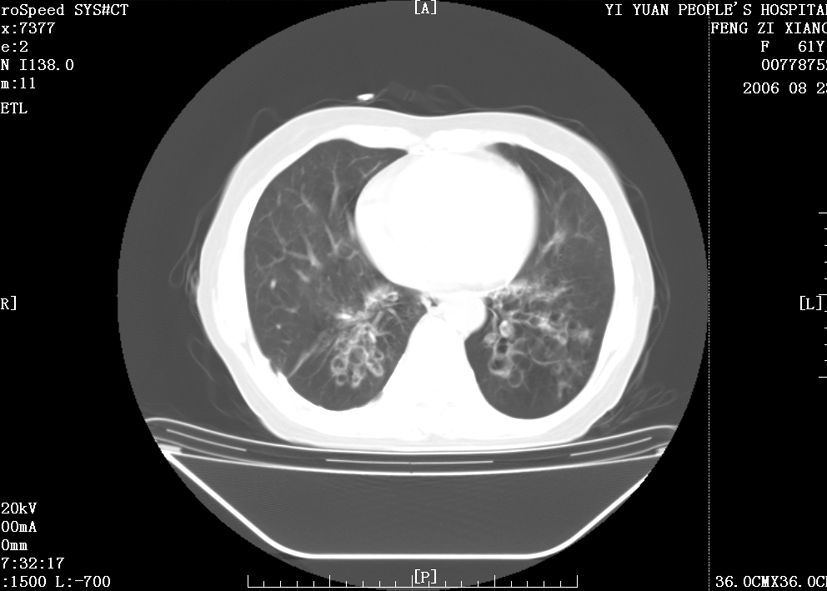
\includegraphics[width=.7\textwidth,height=\textheight,keepaspectratio]{./images/Image00189.jpg}
 \captionsetup{justification=centering}
 \caption{支气管扩张\\{\small 左右肺下叶有从肺门到肺周排列的成排和成簇的囊腔}}
 \label{fig9-6}
  \end{figure} 

除上述典型表现外,还有以下表现:①支气管壁增厚;②支气管内黏液嵌塞;③伴肺叶或段的萎陷,继发于支气管周围纤维化的瘢痕;④可同时伴有肺炎性实变;⑤可同时见肺血量减少的征象,是与本病有关的病变如闭塞性细支气管炎、局灶性全小叶性肺气肿所致。

\textbf{【鉴别诊断】}

1.弥漫性肺纤维化:因肺弹性阻力及胸腔内负压的增加,支气管可呈特征性的“塞钻状”扩张表现,但这种牵引性支扩与常见的支扩病因不同,也无相似症状。

2.组织细胞增生症:有时可见似支气管扩张的囊状改变,多代表空洞性肉芽肿。病变多位于上、中叶,并伴有结节。

3.巨气管支气管症:位于中央部,无支气管壁增厚有助于鉴别。

4.卡氏肺囊虫肺炎、多发性空洞性肺肿瘤尤其是来自肺泡癌者,也可误为支扩。但这些病变无连续性。

5.还应注意下列因素:①在肺血流量减少、肺动脉狭窄时可出现假印戒征;而肺血流再分配和肺动脉高压时血管扩张亦可出现假阴性;②支气管哮喘患者发现36%的肺段支气管内径大于伴行肺动脉,但从无大于1.5倍者;③由于支气管分叉与肺动脉分叉不在同一平面,也可显示支气管内径大于伴随的肺动脉。

\subsection{支气管黏液栓塞}

黏液栓塞是橡皮样黏稠的痰栓塞于支气管内,一般见于肺段或亚段支气管。

\textbf{【病因病理】}
主要见于哮喘病,有时见于过敏性曲菌病、黏稠物阻塞症(Muconvisidosis)或慢性支气管炎患者。黏液栓子呈灰绿色,可长达1~3cm,宽1~2.5cm。其所在支气管管腔因栓子的不断扩大而扩张,管壁可有感染、重者软骨破坏等。

\textbf{【临床表现】}
可无症状,而偶然发现。有的可表现为发热、咳嗽,干咳或有黏痰,胸痛或咯血。有的可咳出橡皮样质地的痰栓。

\textbf{【CT表现】}
黏液栓塞的支气管与CT扫描层面平行时呈V形、Y形或多个分支条状、手指状、一串葡萄状稍高密度灶,尖端指向肺门;支气管与扫描层面垂直时呈结节状影像。其CT值约为-5~20Hu,黏液浓缩后CT值约30~50Hu。因有侧支通气往往无肺不张。如有不张,在不张的肺内黏液栓可呈上述条状、分支状等低密度灶。黏液栓塞可引起阻塞性炎症、脓肿或支气管扩张。

\subsection{支气管结石}

支气管腔内有钙化物质存在称为支气管结石。本病为少见病。临床表现为咳嗽、咳痰、咯血丝。

\textbf{【病因病理】}
多与感染有关。在欧美以组织胞浆菌引起者多见。我国则以结核病引起者常见,其次为肺炎、支扩、肺脓肿等,极少数为真菌病、寄生虫感染所致。结石成分85%~90%为磷酸钙,10%~15%为碳酸钙。

来源:①最多见的是钙化的淋巴结向支气管穿破;②支气管软骨坏死钙化,而后与支气管分离脱落入管腔内;③吸入的支气管异物形成结石核心而继发钙化;④支气管扩张时富于钙盐的分泌物滞留与凝结;⑤肺内钙化灶向支气管腔内穿破。

\textbf{【临床表现】}
可有咳嗽、咳痰等呼吸道感染症状,或咳血丝痰。有的病人诉有小结石咳出。

\textbf{【CT表现】}
支气管腔内颗粒状不规则钙化灶,2~8mm大小,多位于叶或段支气管。连续复查可见单个钙化灶消失或多个钙化灶数目减少,与结石咳出有关。形态和位置的改变可作为该病的诊断依据之一。结石可产生阻塞性肺不张、阻塞性肺炎或黏液潴留。

\subsection{支气管异物}

气管、支气管异物多发生在幼儿,临床多依靠病史、症状和体征及普通X线检查进行诊断。

\textbf{【临床表现】}
临床一般分为4期:①异物进入期:因异物突然刺激,当即出现剧烈咳嗽和气梗;②安静期:异物停留后,症状可暂时减轻或不明显;③阻塞期:由于异物存留和黏膜肿胀,出现喘鸣、气短、阵咳和呼吸困难;④并发症期:并发支气管或肺部感染,有发热、咯脓或血痰等。

\textbf{【X线分期】}
有文献根据病史及X线表现将其分为3期:①双向通气期:异物进入24小时内,无阳性X线表现;②活瓣期:异物吸入气管内12~48小时,X线示患侧肺气肿,纵隔向健侧移位;③活瓣关闭期:超过48小时,X线示患侧肺不张,纵隔向患侧移位。但影响X线表现的因素还有异物的大小、形态和性质。

\textbf{【CT表现】}

1.异物本身:有文献报道有约20%~35%可直接显示异物,异物可附着于管壁上或嵌顿于管腔内(图\ref{fig9-7})。

\begin{figure}[!htbp]
 \centering
 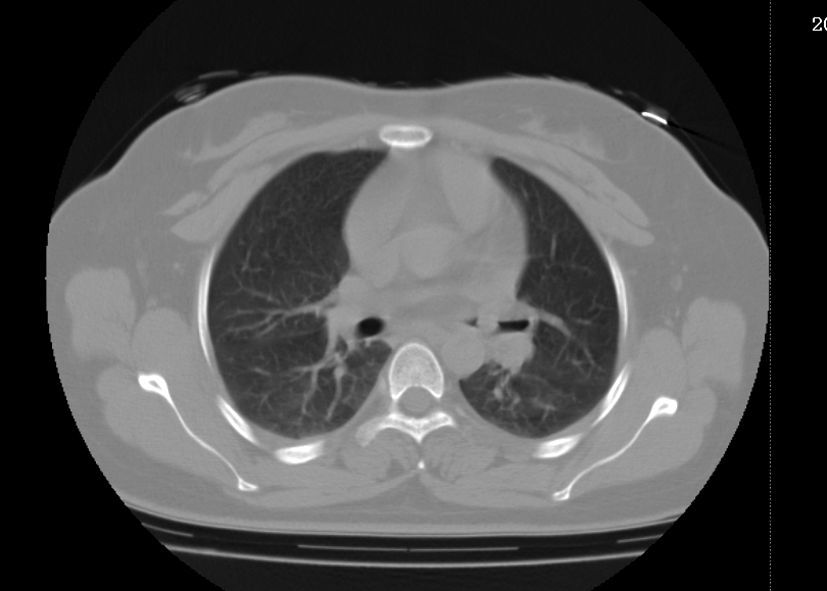
\includegraphics[width=.7\textwidth,height=\textheight,keepaspectratio]{./images/Image00190.jpg}
 \captionsetup{justification=centering}
 \caption{支气管异物\\{\small 左侧支气管内有结节状高密度灶,为吸入的大蒜碎块}}
 \label{fig9-7}
  \end{figure} 

2.局限性支气管阻塞:近80%可显示此改变,其下方支气管充气或轻度扩张。

3.纵隔移位及双边影:多向健侧移位,并因纵隔摆动而产生双边征。异物处于活瓣期时,患侧多有肺气肿,纵隔向健侧移位。活瓣关闭期,患侧多有肺不张表现,纵隔向患侧移位。

4.胸壁双边影:当患侧肺气肿较重时,胸廓的呼吸运动减弱,而健侧的呼吸动度较大,患者正在呼吸时扫描易出现双边影,且说明异物在无双边影的一侧。

5.肺气肿:主要在活瓣期出现。活瓣关闭塞期亦可出现且较重,但活瓣关闭期多为肺不张表现。

\subsection{支气管损伤}

\textbf{【病因病理】}
本病可因挫裂或穿通伤引起,造成大气管的完全断裂或不完全断裂。挫裂伤造成的断裂好发于气管隆嵴下2cm左右处。

\textbf{【临床表现】}
患者咳嗽、咯血及呼吸困难。因有张力性气胸存在,产生广泛纵隔、皮下气肿,尤以颈部的气肿为著。

\textbf{【CT表现】}
①气胸和纵隔气肿:外伤病人如有张力性气胸和纵隔气肿而无胸腔积液,应首先想到气管、支气管裂伤;②环绕气管、支气管的低密度气带影;在周围气体衬托下可直接显示气管、支气管的破口或断裂的部位、形态;③严重的支气管完全断裂可使一侧不张肺完全脱离肺门,卧位时可向外上移位;④急性期和慢性期均可发生肺不张;⑤可合并胸骨骨折和第1~3肋骨骨折;⑥可有气管狭窄、气管食管瘘、纵隔炎或支扩等并发症。

\subsection{主支气管肿瘤}

\textbf{【病理】}

1.良性肿瘤:占成人原发性支气管肿瘤的不到10%。主要有乳头状瘤、纤维瘤、平滑肌瘤、错构瘤、软骨瘤、神经纤维瘤、脂肪瘤等。

2.恶性肿瘤:①成人原发性气管肿瘤中90%为恶性肿瘤。最常见的为鳞状细胞癌和腺样囊性癌(分别占55%和18%~40%),少见的有腺癌、类癌、黏液表皮样癌、软骨肉瘤、平滑肌肉瘤及恶性淋巴瘤等。②主支气管最常见的是非小细胞肺癌,所谓“腺瘤”通常主要指类癌。③气管转移瘤可继发于食管、甲状腺、纵隔和肺等恶性肿瘤的血行转移或直接侵犯。此外,还可继发于肾癌、黑色素瘤,其他腺癌和肉瘤等。

\textbf{【临床表现】}
早期为间断性咯血,但常无任何症状。肿瘤增大后因气管阻塞而表现憋气、气喘、呼吸困难和肺内感染。恶性者转移至邻近脏器可出现相应症状。

\textbf{【CT表现】}

1.良性肿瘤:向腔内突出的孤立的、直径<2cm、边缘光滑的圆形结节。气管壁一般无增厚、受侵。肿瘤位于远端时可阻塞主支气管引起肺不张及炎症。软骨瘤密度较高;错构瘤具有骨、软骨及脂肪的CT值;脂肪瘤呈脂肪密度。

2.恶性肿瘤:多位于气管中下部,近半数位于气管中下1/3处。肿瘤早期阶段呈向腔内突出的息肉状或结节状软组织影,结节基底较宽、无蒂,可见气管壁轻度增厚。病变进展形成气管内较大的肿块,管壁明显增厚,可累及管壁一部分或呈环状生长。病变后期向气管周围浸润、软骨破坏,并形成气管外肿块。发生于主支气管者主要表现为肺门肿块和阻塞性改变(见本章第十五节肺肿瘤之图\ref{fig9-24}A、B)。约30%~40%直接侵犯纵隔引起纵隔及肺门的淋巴结增大;颈部气管肿瘤可直接侵犯喉部;胸膜转移可引起胸水及胸膜结节。

\textbf{【鉴别诊断】}
①恶性肿瘤与良性肿瘤的主要区别为管壁增厚,无管壁增厚时与良性肿瘤不易鉴别。②气管结核的狭窄范围长,可累及主支气管及叶、段支气管,肺内有结核灶。

\section{肺先天性疾病}

\subsection{肺不发育和肺发育不良}

\textbf{【病理】}
胚胎在3~24周的时期发育异常可引起肺发育畸形,可合并半椎体、肾不发育等其他肺外畸形。①肺不发育:如一侧肺完全缺如,称为一侧肺不发育。②肺发育不良:是指肺组织形态类似胚胎早期阶段,未发育为成熟的结构。可局限于一个肺叶、肺段或一侧肺脏。常合并先天性支气管扩张或闭锁。③发育不良综合征:一侧肺发育不良合并同侧血管畸形称为肺发育不良综合征。

\textbf{【临床表现】}
可无症状而偶然发现,患侧胸廓变小或正常。一侧肺不发育,呼吸音消失,肺发育不良合并感染可有发热、咳嗽、咳痰等症状。

\textbf{【CT表现】} 一般采用普通平扫检查。

1.一侧肺不发育:患侧胸腔密度升高,是移位纵隔、心脏大血管等形成的影像。上胸腔可见健侧疝入之肺组织形成的含气低密度区。患侧主支气管缺如,或可见部分残存。患侧胸廓小、肋间隙变窄、膈肌升高。较小患儿患侧胸廓缩小可不著。对侧肺脏血管增粗、分布稀疏。增强扫描可见患侧肺动脉缺如。

2.肺发育不良:一侧、一叶肺密度增高,体积缩小。一侧支气管变细、分支少;增强扫描可见肺动脉缺如或细小。密实肺组织内可见含气支气管影像及薄壁空腔,有的可见支气管狭窄及远端的支气管扩张。合并支气管闭锁(好发于上叶)时,其远端可有黏液栓形成。

一侧肺不发育诊断不难,但肺发育不良有时不易与肺不张及肺炎区别。

\subsection{肺发育不良综合征}

本病是一种少见的先天性发育畸形,几乎都发生于右侧。

\textbf{【病理】}
其特征性改变是异常增粗的下肺静脉呈弧状沿右心缘引流到下腔静脉或毗邻的右心房,形成所谓的“弯刀征”。若合并右肺动脉、右肺发育不良和心脏右移(旋),称为“弯刀”综合征或肺发育不良综合征。病灶由体循环动脉供血,故有学者把它作为肺隔离症的变异之一。其上述特征在同一病例并非都能出现。

\textbf{【临床表现】}
一半以上病人无症状,但肺发育不良较严重或伴先心病的病例在婴儿期即可有明显的呼吸困难和反复的感染。

\textbf{【CT检查的价值】}
①明确增粗弯曲的肺静脉引流途径;②证实异常的体循环血供;③显示畸形萎陷的肺叶内稀疏变细的肺血管,发现肺和肺动脉的发育不良。

\subsection{先天性大叶性肺气肿}

\textbf{【病因病理】}
为先天性支气管发育异常如软骨发育不良、腔内黏膜增生、狭窄等,也可为未闭的动脉导管或腔外迷走血管压迫等。以单叶肺气肿最常见,约占95%以上,其中左上叶约占45%,右中叶约占30%,右上叶约占20%,两叶及以上的肺气肿约占5%。病理特征为受累肺叶过度充气扩张而不伴有肺泡间隔的破坏。

\textbf{【临床表现】} 多发生于生后6个月内,呼吸困难为常见症状。

\textbf{【CT表现】}
病变肺叶过度充气膨大而密度减低,病变区肺纹理稀疏。邻近肺叶常因受压而膨胀不全,纹理聚拢。患侧胸腔增大,纵隔向健侧移位。

\textbf{【鉴别诊断】}
诊断时应注意:①肺发育不良:勿将压迫不张的肺看作发育不良,把肺气肿的病叶看作代偿性气肿。肺发育不良纵隔向患侧移位,无压迫性征象。②特发性单侧透明肺:与肺气肿相似,密度低,但患侧肺容积正常或缩小,肺纹理细小或普遍稀疏。肺门血管亦示细小,纵隔及邻近病变的肺叶移向患处而与肺气肿不同。

\subsection{特发性单侧透明肺}

本病又称为单侧肺过度透明症、Swyer-James综合征。

\textbf{【病因病理】}
可为先天性一侧肺动脉发育不全所致,也可以是病毒、细菌、支原体等感染所致,可影响一叶或一侧肺,左肺多于右肺。国外文献认为与病毒、细菌、支原体等所致的感染后闭塞性细支气管炎密切相关,婴儿期和儿童早期患急性细支气管炎可导致终末细支气管和呼吸性细支气管的破坏,并影响肺泡芽的正常发育(因为肺泡的发育一直持续到8岁)。肺泡芽的破坏使病变区肺循环减少,为维持正常肺容积,段支气管和近端细支气管过度充气扩张,出现肺气肿。肺动脉发育不全可能为继发,也有学者认为可能为原发。病理主要呈闭塞性细支气管炎的慢性炎性改变,阻塞支气管的远端气道和气腔扩张。

\textbf{【临床表现】}
好发于儿童,亦可见于青少年和成年人,以女性多见。表现为反复咳嗽、咳痰、喘息和咯血,少数无明显症状。主要与有无支扩和扩张的类型有关。

\textbf{【CT表现】}
可为一侧肺或仅累及一叶或一个肺段。表现为密度减低,其内血管纹理细小,同侧肺门缩小,但与肺气肿不同的是肺容积缩小或正常。增强扫描对细小肺血管的显示更优,尤其易于显示肺门缩小、中央肺动脉变细。

此外,X线可见吸气时纵隔向患侧移位,呼气时向健侧移位;肺动脉造影可见患侧肺动脉细小;同位素扫描通气及灌注均下降。这些表现有助于进一步确诊。

\textbf{【鉴别诊断】}
注意排除支气管内病变引起的不完全阻塞、一侧肺大泡或气胸、单纯肺动脉发育不全、肺动脉栓塞等。

\subsection{先天性肺囊性腺瘤样畸形}

本病是一种肺的发育异常性疾病,有文献认为是肺错构瘤样囊性发育畸形。病变最早发生在胚胎第5~10周。

\textbf{【病理】}
由不同大小和分布的、异常增生的毛细支气管及肺泡样结构组成,部分增生呈乳头状隆起。通常与正常支气管无交通而大多经侧支通气,大部分由肺循环供血。

可分为3型:Ⅰ型:占65%,由大小不等的囊构成,但其中含有单个或数个厚壁大囊(囊径3~10cm);Ⅱ型:约占25%,由为数众多的均匀分布的小囊组成(囊径0.5~3.0cm);Ⅲ型:约占10%,由大块实性成分组成,其内有肉眼难辨的毛细支气管样小囊(囊径<0.5cm)和不规则的细支气管样结构。Ⅱ型和Ⅲ型可合并先天性心血管、肾、小肠和骨骼系统畸形。

\textbf{【临床表现】}
可发生于任何年龄,1岁以下儿童多见。大多于生后6个月内出现症状,常见为呼吸窘迫,以后可出现咳嗽、发热和反复肺部感染。Ⅰ型预后好;Ⅱ型预后取决于并发畸形的多少及严重程度;Ⅲ型并发畸形多,往往死于宫内,预后差。

\textbf{【CT表现】}
本病局限于单一肺叶者占95%,累及双肺者不超过2%。下叶发病率最高,中叶最低。病灶可累及一叶或两叶。典型表现为一团多发薄壁含气的囊状结构,囊通常大小不等;部分呈囊实性表现。部分病灶内可见液气平面影,但并不代表感染;继发感染时液气面更为常见,且可见渗出灶。必须重视的是病灶均有占位效应,致纵隔向对侧移位甚有意义。少数可恶变成间充质肉瘤,使病灶呈软组织密度块。

\textbf{【鉴别诊断】}

1.肺囊肿:常为单个或多个囊腔聚集,一般壁较光滑,继发感染的几率高,因此多含气液面。肺囊肿常与肺囊性腺瘤样畸形鉴别困难,但多无纵隔移位或因伴肺发育不良而使纵隔向患侧移位;而囊性腺瘤样畸形多有占位效应,使纵隔向健侧移位。此外,对囊腔不规则、壁内有息肉样突起或大囊周围伴有较多小囊样结构者,应考虑囊性腺瘤样畸形可能。

2.肺隔离症:有较特异性的发病部位,即多见于下叶尤其左下叶后底段,增强CT扫描发现来自体循环的异常供血可确诊。但肺隔离症可伴发先天性肺囊性腺瘤样畸形,且以Ⅱ型多见。

3.囊状支气管扩张:小儿较少见,可为先天性,易继发感染。可表现为成簇的含气及气液面的囊腔,囊腔大小较一致,按肺段分布。HRCT可见囊腔与支气管相通,患肺体积可缩小。

\subsection{肺隔离症}

本病又称支气管肺隔离症。合并与支气管或食管异常交通者,称为先天性支气管肺前肠发育畸形。支气管肺隔离症是指一部分肺发育不全,无呼吸功能,与相邻肺叶的正常部分相隔离。

\textbf{【病理】}
病变的肺组织不能由正常肺动脉供血而来自主动脉分支,病变部失去正常肺组织的形态结构而呈囊状、囊实性或实性的肿块。肺隔离症的供血来自胸、腹主动脉及其分支。

分型:可分为3型:①肺叶内型:占75%。多位于下叶后基底段,尤以左侧多见(60%~90%)。肺叶内型病变区与同叶正常的肺组织被同一层胸膜所包裹。②肺叶外型:为副叶或副肺段,有独自的脏层胸膜,90%位于左侧。与膈关系密切,可位于膈上、膈下甚至包围在膈肌中。还有位于左上纵隔旁的报道。肺叶外型可伴有膈肌发育异常(如膈疝、膈膨升)、隔离肺与胃肠道瘘,以及骨骼系统和心脏发育异常。③混合型:罕见。

\textbf{【临床表现】}
20岁左右的青年人多见。主要表现为反复发生的肺部感染症状,如咳嗽、咳痰、咯血、胸痛等。肺叶外型可无肺部症状,而因其他合并畸形就诊。

\textbf{【CT表现】} 取决于其内是否含气。

1.肺叶内型:①实质型:见于隔离肺组织与支气管不相通时,表现为团块状或分叶状、边缘清楚、密度均匀的致密影。常位于下叶后基底段,其长轴指向内后方,提示与胸主动脉或腹主动脉有联系。合并感染则边缘模糊,此型偶有恶变。②囊肿型:见于与支气管相通者,显示为含气的、壁薄的、单囊或多囊状影,边缘清楚,内有液平面。

2.肺叶外型:位于膈上或膈下的胸部或腹部块影。

3.增强扫描:多数肺叶内型和少数肺叶外型病变区呈不规则强化,以囊状结构之间的实质性部分强化明显。增强扫描对发现异常血管更为敏感,它与隔离的肺组织相连(图\ref{fig9-8})。在部分病人的多轴位或三维重建中,可清晰显示异常供血的动脉和引流静脉的起止部位,有利于诊断和鉴别诊断。



\begin{figure}[!htbp]
 \centering
 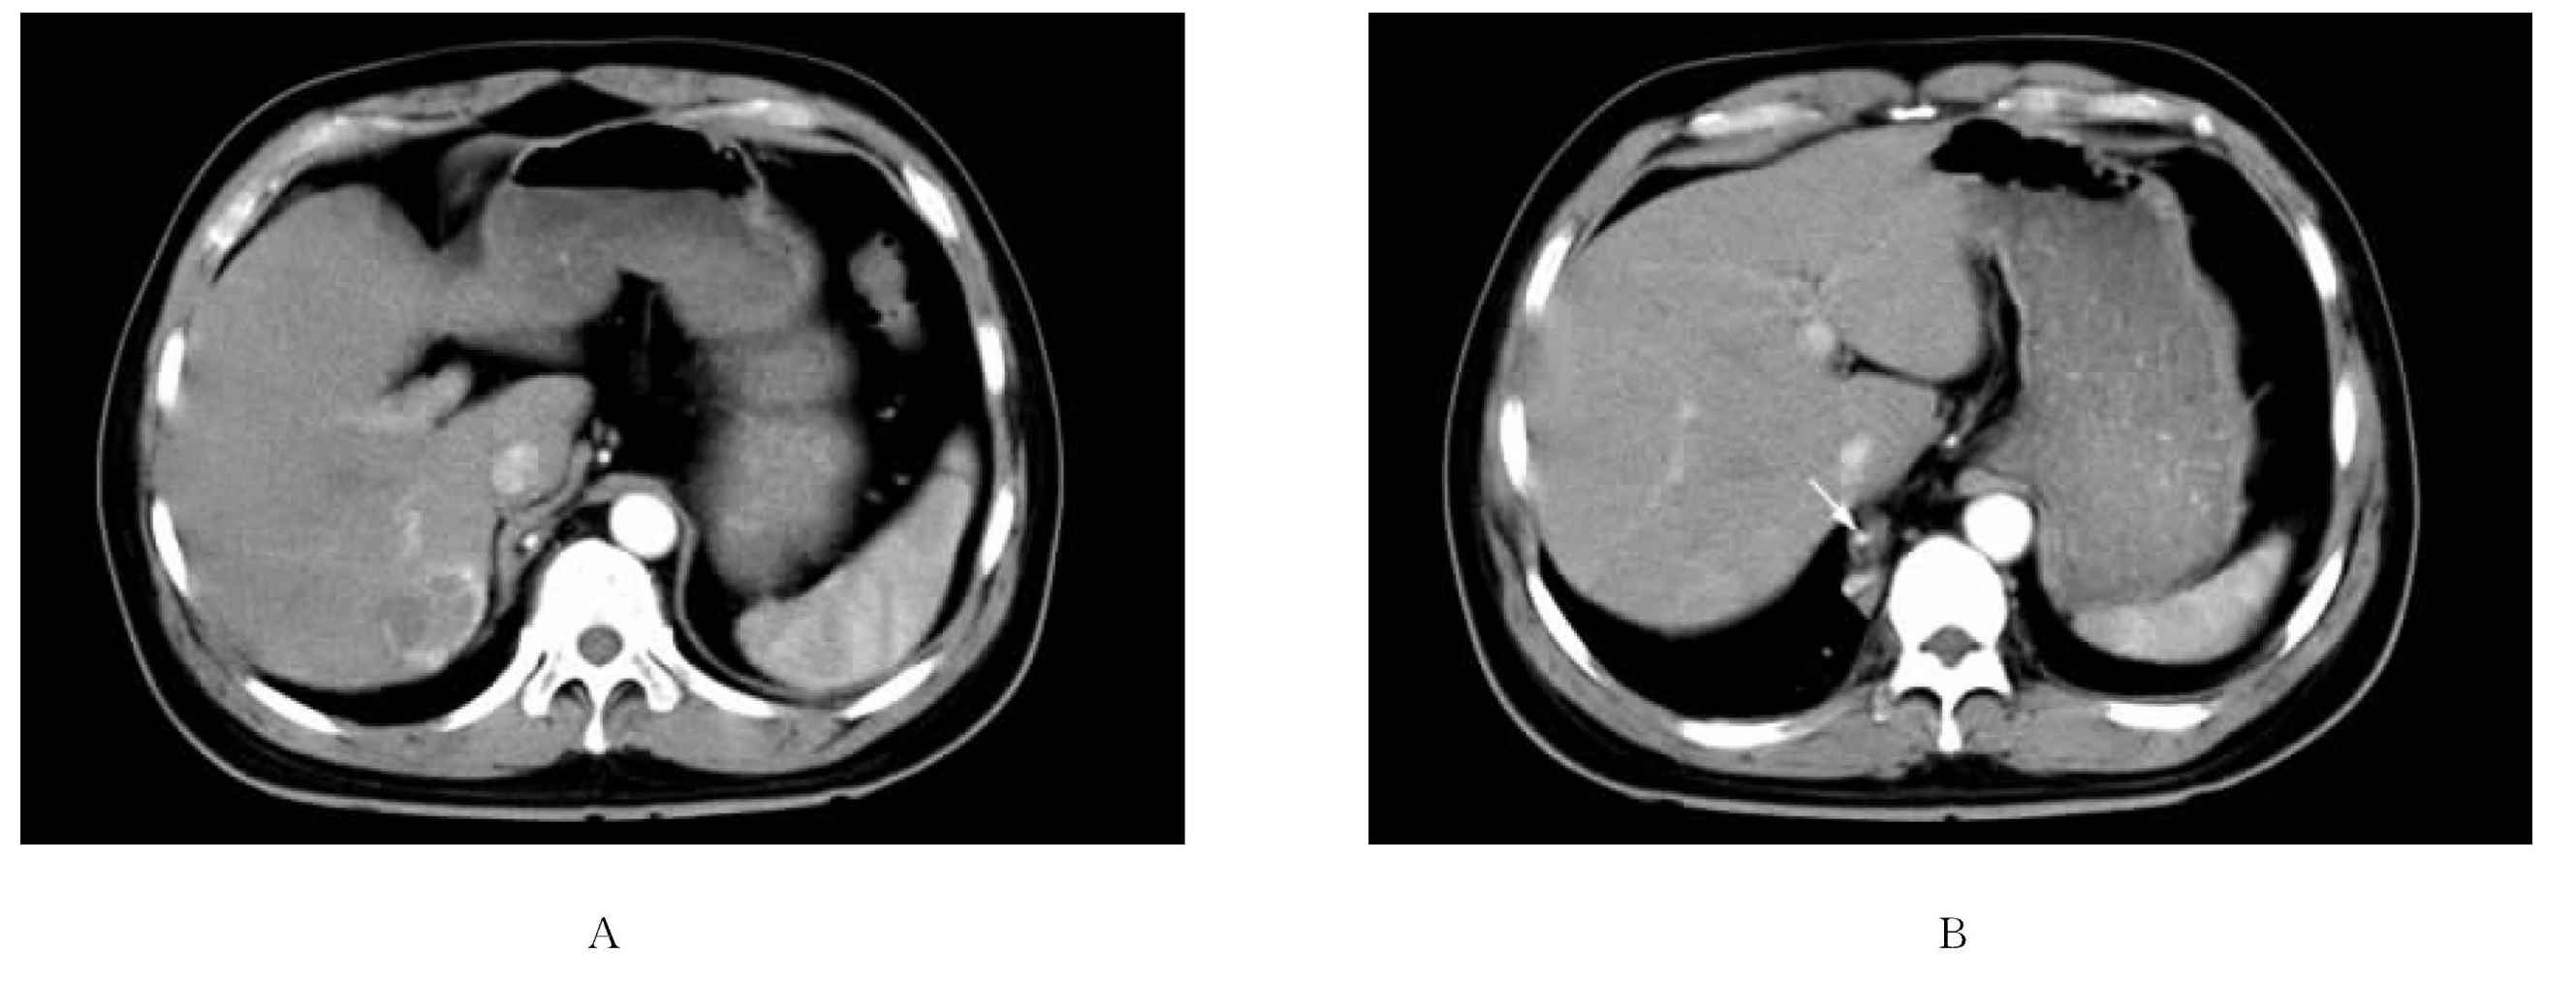
\includegraphics[width=.7\textwidth,height=\textheight,keepaspectratio]{./images/Image00191.jpg}
 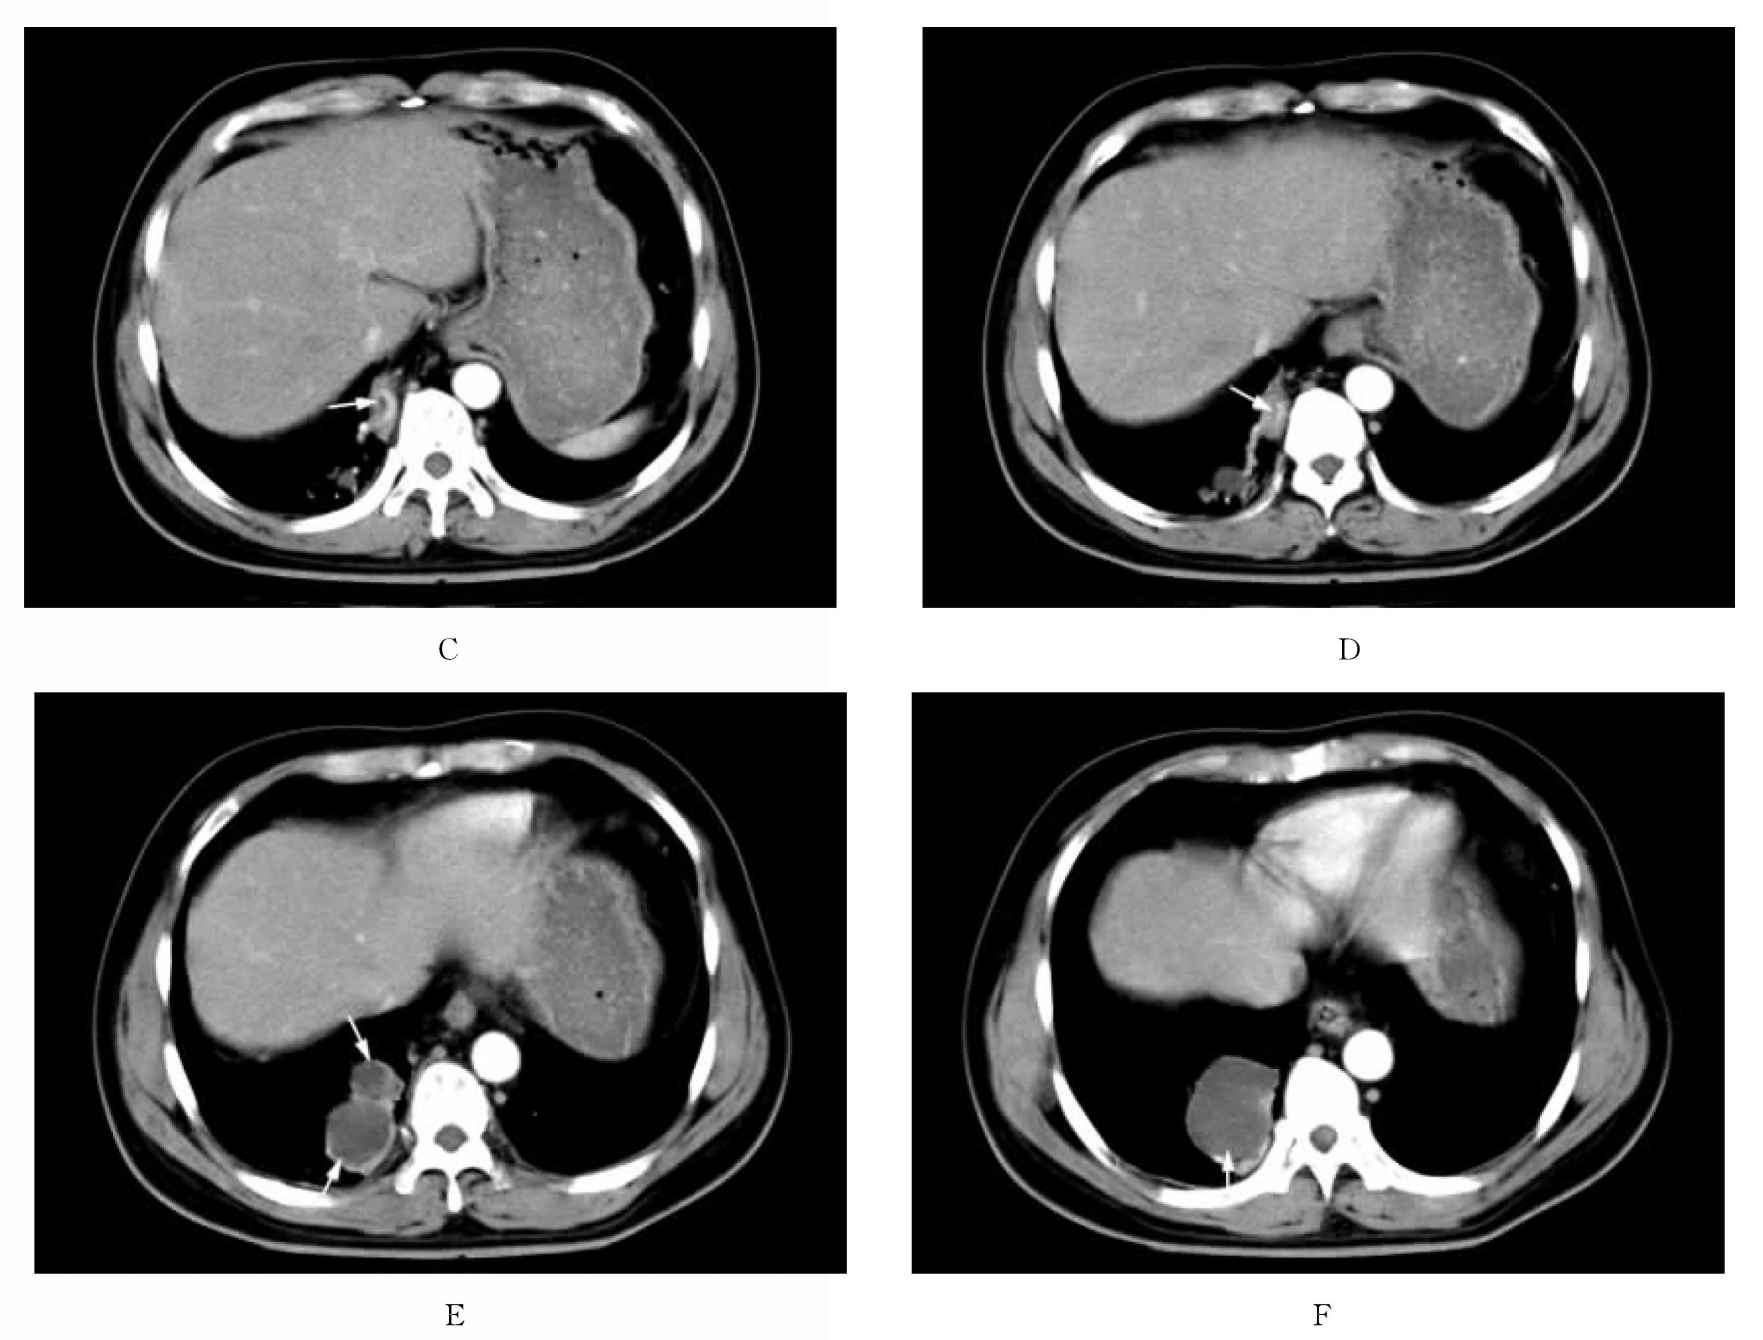
\includegraphics[width=.7\textwidth,height=\textheight,keepaspectratio]{./images/Image00192.jpg}
 \captionsetup{justification=centering}
 \caption{肺隔离症\\{\small A~F为由下向上的连续层面。A~D可见由膈下向上伸延的异常供血动脉(箭);E、F可见右侧下叶后底段边缘强化的囊状水样密度灶(囊肿型隔离肺)}}
 \label{fig9-8}
  \end{figure} 

\textbf{【鉴别诊断】}

1.肺囊肿:多呈单囊性,而肺隔离症呈单囊者相对少见。与异常强化的血管相连是肺隔离症的典型特征。

2.肺脓肿:肺隔离症合并感染表现与肺脓肿相似。一般急性肺脓肿周围有较重的炎性改变,而且经抗炎治疗吸收可资鉴别。

3.膈疝:疝入胸部的胃肠道可与肺隔离症表现相似,但气体衬出的胃肠道黏膜、服泛影葡胺后CT扫描及钡餐检查可确诊。

4.囊状支气管扩张:多呈大小不等的多发囊状,常合并肺不张,咯血症状明显。HRCT可见囊腔与支气管相通,患肺体积可缩小。

\subsection{肺动静脉畸形}

本病命名繁杂,又称为肺动脉瘘、肺动静脉瘤、肺血管瘤等,是一种较少见的先天性血管畸形,由胎儿期毛细血管吻合支持续存在所致。

\textbf{【病理】}
其特征为肺动脉与肺静脉直接相连,其间无毛细血管床。可分为3型:①单纯型:为最常见的类型,供血动脉和引流静脉均为单根。②复杂型:为多支供血动脉和引流静脉。③弥漫型:亦称为毛细血管扩张型,以两肺散在多发的微小动静脉瘤为特征。亦有人将其分为囊状和弥漫型两型,前者又分为单纯型和复杂型。

本病常见于两下肺,以单发多见,两肺同时发生者约占10%~20%。大约60%的病人同时患有遗传性出血性毛细血管扩张症;而患遗传性出血性毛细血管扩张症的病人,仅约15%伴有肺动静脉畸形。肝硬化、血吸虫病、甲状腺癌肺转移及外伤亦可继发肺动静脉畸形。

\textbf{【临床表现】}
本病以中青年多见。表现为运动性呼吸困难、发绀和杵状指为最常见的症状。部分病人可表现为咯血、血胸等。有些患者可无症状,偶然透视发现。若病灶贴近胸膜面可听到心外杂音。

\textbf{【CT表现】}

1.平扫表现:动静脉畸形之“瘤体”:①圆形或椭圆形病灶,可呈分叶状,边界清楚;②复杂型亦可呈大片状致密影,类似肺炎;③肺毛细血管扩张型病灶多而小,直径一般<5mm,呈弥漫分布的许多小结节。

2.增强扫描:上述各型病灶与肺动脉平行强化,引流静脉和左房提早显影。即病灶强化峰值出现的时间与肺动脉和右心室几乎一致,到左心室期病灶强化已开始下降,上述强化特征有利于诊断和鉴别诊断。如强化不明显应考虑“瘤体”内有血栓形成或病灶为非血管性。

3.供血动脉和引流静脉:因血管走行和扫描层面的关系可呈结节状、条状或椭圆形;供血动脉一般较细,强化时间早于“瘤体”及引流静脉。三维重建、多平面重建和CT血管成像有利于显示与肺门相连的血管和发现多发病灶。

\subsection{肺动脉瘤}

肺动脉瘤为肺动脉及其主要分支,甚至周围肺野小分支的管腔局部膨胀。本病极少见。与主动脉瘤相比,其发病年龄要小的多。

\textbf{【病因】}
先天性者见于特发性肺动脉扩张或马凡综合征;获得性者有感染(血管内感染)和外伤两个原因,任何细菌感染引起者称为细菌性肺动脉瘤。此外,还有肺动脉夹层的报道。

\textbf{【临床表现】}
先天性特发性肺动脉扩张者往往无临床症状。有些病人有先心病病史并发细菌性心内膜炎或先有肺部感染史,以后出现呼吸困难、气短等症状,也可有咳血,甚至大咯血而死亡。

\textbf{【CT表现】}
可发生于主肺动脉或左右分支,表现为局限性增粗;在周围肺野则呈单个或多个高密度结节。增强扫描均与肺动脉强化曲线一致。

\subsection{迷走左肺动脉}

本病是一种罕见的先天性畸形,可引起上呼吸道阻塞症状。

\textbf{【病理】}
左肺动脉从主肺动脉发出后向右走行,在气管下端及右主支气管的前上方通过,然后向后、向左在气管和食管之间向左行,到达左肺门。

\textbf{【临床表现】}
多见于婴幼儿。患儿出生后不久即出现喘鸣,喂乳时哭闹及青紫,易患呼吸道感染。

\textbf{【CT表现】}
左肺动脉由主肺动脉发出,行走于右主支气管前上方,然后在气管和食管之间穿过,跨入左肺到达左肺门。右肺上叶可不透亮或过度充气。

\subsection{肺静脉曲张}

本病是指肺静脉进入左房开口部位的瘤样扩张和局限性扩大。

\textbf{【病因病理】}
其病因尚无定论,半数伴二尖瓣病变。大多认为可能系肺静脉的发育异常,可伴肺内或心脏大血管异常,特别是二尖瓣关闭不全。病理示肺静脉进入左房前的一段扩张及扭曲。血管壁变薄,平滑肌萎缩由纤维组织代替,或局部血管壁因有多量纤维组织而增厚。

\textbf{【临床表现】}
可发病于任何年龄,多在30~45岁,性别无差异。多无症状而偶然发现。少数有咯血甚至大咯血。若曲张静脉内的血栓脱落,可引起其他器官的栓塞症状。后天性二尖瓣病变继发者可有相应的症状和体征。

\textbf{【CT表现】}
两下肺内带圆形、椭圆形或管状高密度灶,边缘清晰,略分叶,与左心房关系密切。右肺多于左肺,在右肺常见于下叶的基底静脉的近端,左侧较多见于舌段静脉。增强扫描有明显强化,与左心房CT值接近。

\textbf{【鉴别诊断】}
主要应与肺动静脉畸形相鉴别。肺动静脉畸形与肺动脉强化一致,肺静脉曲张于静脉期显著强化(与左心房一致),且无肺动静脉畸形所见的特征性的伴行动、静脉可予以鉴别。

\subsection{肺部淋巴管扩张症}

本病又称为弥漫性淋巴管瘤病。是较少见的先天性发育异常,可全身淋巴系统广泛受累,或只侵及肺部淋巴系统。它与肺部淋巴管平滑肌增生症(淋巴管肌瘤病)非同一疾病。

\textbf{【病因病理】}
胚胎第12~16周时,肺部各处淋巴组织已发育成熟,且与肺部其他成分比较相对较多。至18~20周时,肺部结缔组织减少,淋巴管亦相应变窄。若此时淋巴管不相应减退,则成为淋巴管扩张症。有时可伴有先天性心脏病及静脉回流受阻。

\textbf{【临床表现】}
本病多见于婴幼儿。可分为早发型和晚发型。前者于出生后几分钟即发生呼吸困难、青紫,多在1~2天或数天夭折。后者多发病于儿童或成年,可表现呼吸困难或因胸水、胸部囊性病变而进一步检查。

\textbf{【CT表现】}
HRCT检查可见:①弥漫性间质改变:小叶间隔、斜裂和水平裂表面以及肺门血管、支气管周围间质增厚,呈网状、结节状改变以及支气管血管束增厚;②磨玻璃样改变及肺实变:代表炎性渗出;③肺内囊肿样改变:呈高密度,代表囊肿样扩张的淋巴管;④胸腔积液:单侧或双侧;⑤有些只表现一般肺部炎症和局限性肺气肿;合并有先心病者可有相应表现。

\section{肺不张}

\subsection{分类}

肺不张表示肺的充气减少、体积缩小,呈部分或完全萎缩状态。

根据病因国内荣独山把它分为:①无力性肺不张;②阻塞性肺不张;③外压性肺不张;④约制性肺不张。

美国James.C.Reed则将其归纳分为:①阻塞性肺不张;②压迫性肺不张;③被动性肺不张;④瘢痕性肺不张;⑤粘连性肺不张。其中②、③相当于国内的外压性肺不张,④相当于约制性肺不张。

\subsection{无力性肺不张}

本病多见于未成熟的胎儿。

\textbf{【病因病理】}
正常胎儿出生时可有部分肺泡未充气,而在以后的几天内逐渐膨胀。如果胎儿在生后因呼吸无力而肺部有较多的肺泡不能充气就造成肺不张。病理为散在的小叶性不张,可涉及肺段、肺叶甚至更大的范围,多见于两侧。

\textbf{【临床表现】}
患儿可有不同程度的呼吸困难,可有紫绀,严重者可很快死亡。

\textbf{【影像学表现】}
可见弥漫性散在分布的粟粒状或颗粒状高密度灶,亦可呈毛玻璃样。其中可见到支气管充气征。本病影像学诊断困难。

\subsection{阻塞性肺不张}

阻塞性肺不张是指气管、支气管气道阻塞,使其供应的肺内气体吸收消失而造成的肺不张。

\textbf{【病因病理】}
阻塞的病因较多,如吸入异物、浓稠的黏液、炎性渗出物、血块、支气管肿瘤、支气管肉芽组织和炎性狭窄等。一般气管完全阻塞后18~24h气体即可完全吸收。长期慢性肺不张易导致纤维化而永久萎缩,有的可并发支气管扩张。肺不张的程度、部位和范围取决于阻塞的部位和程度。

\textbf{【影像学表现】}

1.右上叶肺不张:①轻度收缩时,其形态基本保持不变,仅向上并向前移位。②右上叶体积明显缩小时,在纵隔旁呈尖向肺门的楔形高密度影,其外侧和后侧为过度膨胀的右中叶和右下叶。右下叶背段的部分肺组织位于不张的后内缘与纵隔间。③当有胸膜粘连时,则限制了其移位的方向而向粘连处移位。

2.右中叶肺不张:右中叶呈五面体形态。不张时呈底向右心缘、尖向外的三角形高密度影;体积明显缩小时可呈带状或线形。相应的水平裂和斜裂可移位。但相邻肺叶的代偿性肺气肿不明显。

3.右下叶肺不张:不张的下叶向后纵隔方向收缩。明显不张时,不张的下叶靠近脊柱,斜裂明显向后方移位(图\ref{fig9-9}A)。

4.右上叶和中叶联合肺不张:右上、中叶向前内移位,位于纵隔旁。在主动脉上方层面,前部为不张的影像,后半部为膨胀的右下叶;在气管隆突平面肺不张呈三角形,与纵隔及前胸壁相连,尖端位于肺门侧。

5.左上叶肺不张:不张的上叶向前上方移位。左上叶一部分与前胸壁接触,呈尖向后、底边向前的楔形或三角形(图\ref{fig9-9}B)。其上方为过度膨胀的左下叶。不张的左上叶与主动脉之间的间隙被过度膨胀的下叶一部分占据,呈舌状。

6.左下叶肺不张:向后纵隔方向收缩,靠近降主动脉和脊柱。

7.肺段性(或亚段性)肺不张:形态多样,可呈线形、条带形、楔形、类圆形等阴影。其引起肺体积和周围器官变小。分析时应注意邻近肺段有无代偿性肺气肿和附近的叶间裂有无移位。

8.一侧性肺不张:可见一侧肺密实、体积缩小,纵隔向患侧显著移位(图\ref{fig9-9}C)。

\begin{figure}[!htbp]
 \centering
 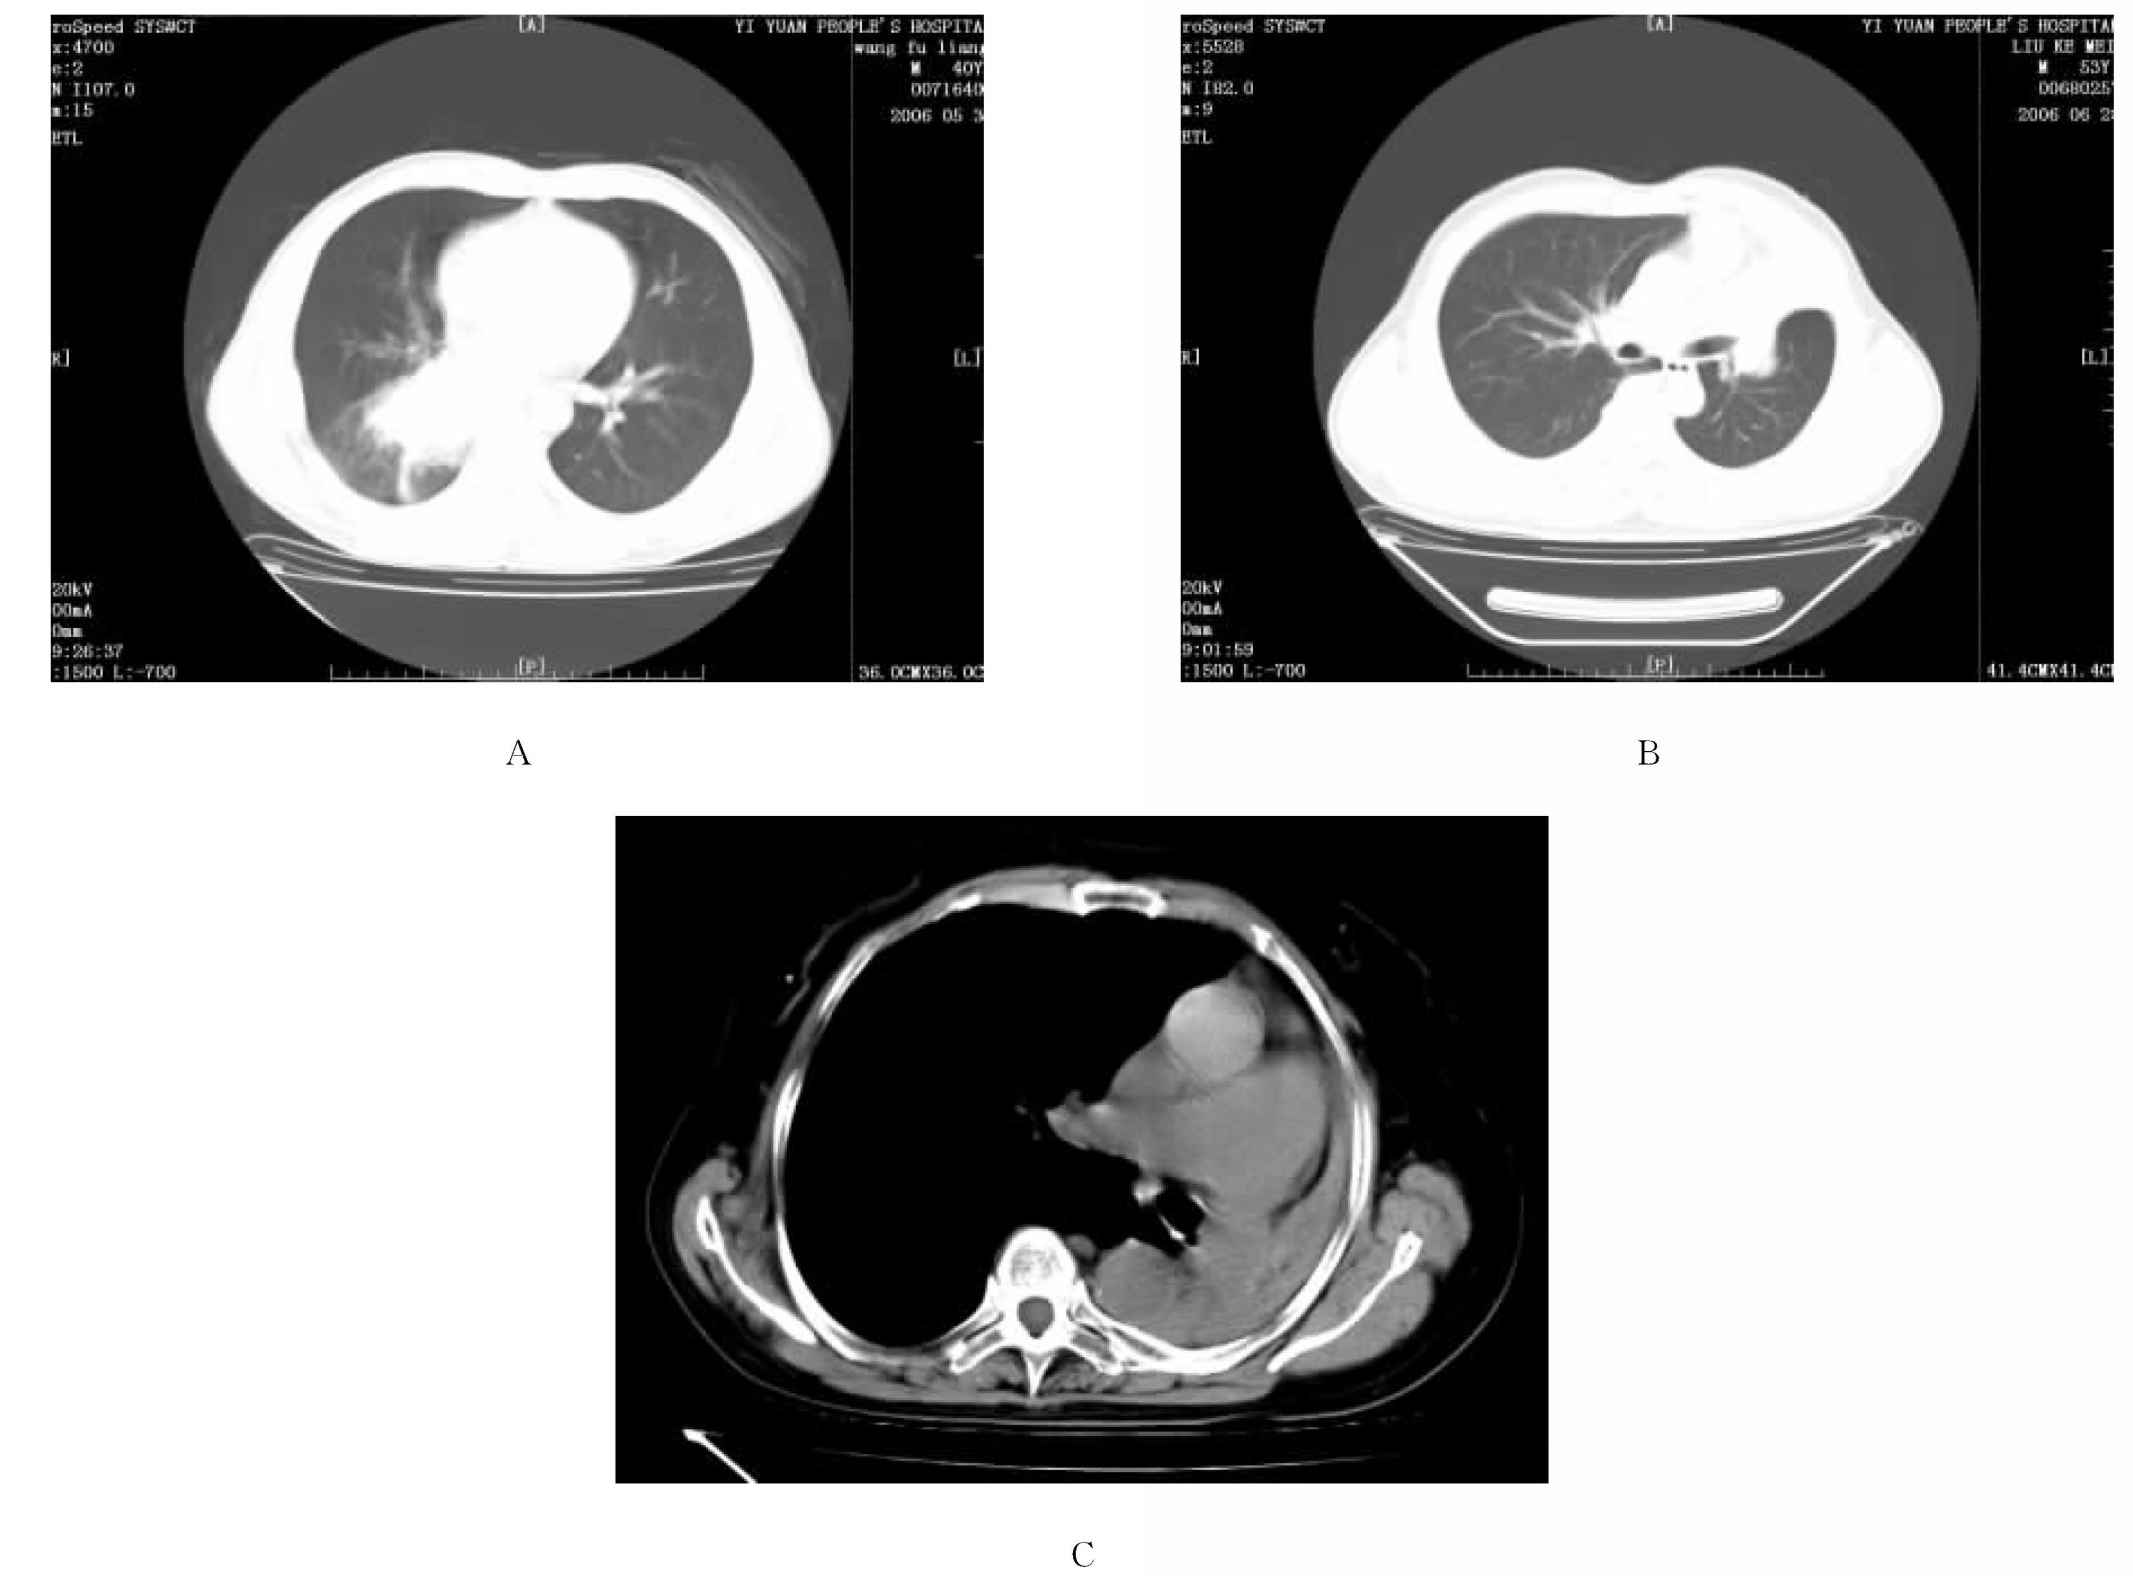
\includegraphics[width=.7\textwidth,height=\textheight,keepaspectratio]{./images/Image00193.jpg}
 \captionsetup{justification=centering}
 \caption{肺不张\\{\small A~C非同一患者,均为肺癌所致。A.右下叶肺不张;B.左上叶肺不张;C.左肺一侧肺不张}}
 \label{fig9-9}
  \end{figure} 

此外,在分析不张时应注意其密度的变化。支气管充气征常见于结核或炎症;支气管液相(其密度略低于不张肺组织)多见于中央型肺癌;其内如见不规则钙化、空洞和支扩多见于肺结核。

\subsection{被动性肺不张和外压性肺不张}

\subsubsection{压迫性肺不张}

本病是指肺内占位性病变压迫邻近肺组织使其不能充气而引起的不张。原发病变可以是周围型巨大肿瘤,也可以是间质性肉芽(如结节病)的大量积聚所致。同样,淋巴瘤细胞在肺间质内的大量积聚也可引起广泛的肺压迫。

\subsubsection{被动性肺不张}

本病又称为松弛性肺不张,是胸膜腔内压力的改变所造成的肺萎缩。其病因主要为胸腔积液和气胸(图\ref{fig9-10})。

\begin{figure}[!htbp]
 \centering
 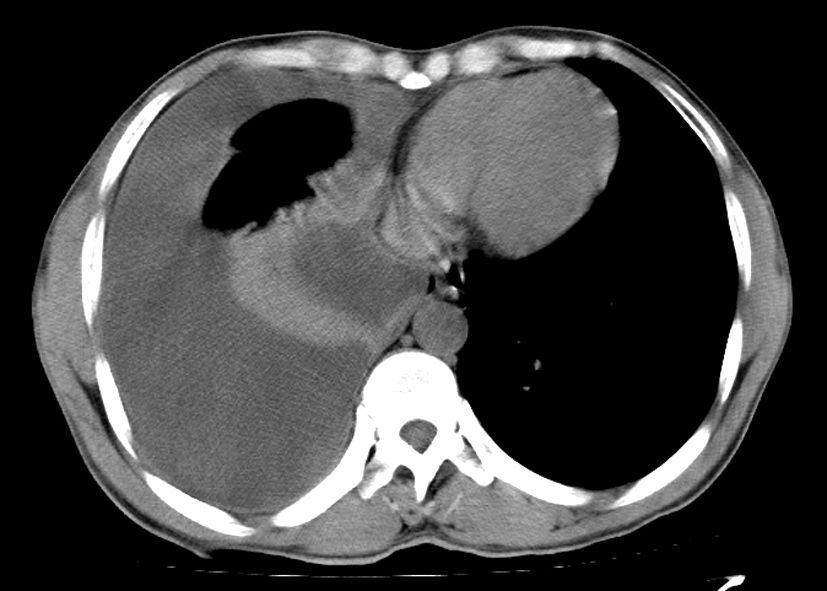
\includegraphics[width=.7\textwidth,height=\textheight,keepaspectratio]{./images/Image00194.jpg}
 \captionsetup{justification=centering}
 \caption{外压性肺不张\\{\small 右侧胸腔大量积液,近肺底部有弧形被压迫不张的高密度肺组织}}
 \label{fig9-10}
  \end{figure} 

\subsubsection{外压性肺不张}

本病是压迫性和被动性不张的总称。似乎把肺不张分为被动性、压迫性是人为的,但它把注意力集中在产生肺萎缩的原因上,就是说不张是肺内还是胸膜腔内病变所引起。

\subsection{瘢痕性肺不张}

瘢痕性肺不张即约制肺不张。是胸膜严重增厚、胸壁的固定或肺泡间和间质间隙内的纤维化、瘢痕形成,使肺组织失去弹性,使呼吸受到限制而引起的部分性肺不张。最常见于结核。

\textbf{【影像学表现】}
瘢痕性肺不张与阻塞性肺不张有时表现相似,但合并有粗大网状影。瘢痕性肺不张的肺容积减少亦可发生于间质纤维化病变(如矽肺、硬皮病、特发性间质纤维化和脱屑性间质性肺炎等)。但间质性病变所致的容积减少,单纯的表现为密度最高、血管聚集和膈肌升高,这一表现被误认为是主动性吸气不足,通常不认为是肺不张。

\subsection{粘连性肺不张}

当肺泡表面粘连在一起时,就可产生粘连性肺不张。该类型肺不张主要见于两种疾病:新生儿肺透明膜病和肺栓塞。其粘连形成的原因推测为表面活性物质的缺乏所致。

\subsection{盘状肺不张}

它是亚段性肺不张的一种特殊X线形态。

\textbf{【病因】}
这种不张大多由于该肺部呼吸障碍所致,往往与横膈运动减弱密切相关,因为此时少量的分泌物可使支气管阻塞,引起亚段性肺不张。可见于膈下病变、腹部病变、急性胸膜炎引起的膈动度减弱,肺梗死亦常并发本症。

\textbf{【X线表现】}
呈2~6cm长,厚度相对较扁的条状或盘状密度增高影,边缘清晰。多见于膈顶上方,呈横行。结合横膈的位置与动度等甚有诊断价值。

\textbf{【CT表现】}
呈条状、楔形或椭圆形高密度灶,边缘相对较清晰。其诊断价值不如X线,但对膈下或腹部病变所致者可提供更多的诊断依据。

\subsection{圆形肺不张}

本病又称为球形肺不张、折叠肺。是一种特殊类型的局限性肺不张,因呈圆形或球形而得名。

\textbf{【病因】}
一般认为游离的胸腔积液是发生本症的必要条件,积液吸收后有部分呈被动性不张状态的肺组织,因受周围增厚胸膜之固定不能复张而形成圆形肺不张。

\textbf{【CT表现】}
呈圆形、类圆形肿块,亦可呈逗点状、楔状、不规则分叶状。大小不等,一般约2.5~5.0cm大小。常位于胸膜下,以下叶外底段或背段多见,偶可位于膈面或上叶。其内可见支气管充气征。块影附近广泛的胸膜增厚是一个重要征象。最特殊的表现是靠近块影内下缘的肺血管和支气管扭曲呈弧形,先达肺底部,然后向上弯曲延伸,颇似彗星的尾部,故称为彗星征,是其较特征性的表现。

\section{肺气肿}

\subsection{分类}

肺气肿主要指肺脏终末细支气管远端部分,包括呼吸性细支气管、肺泡管、肺泡囊和肺泡的过度充气,或由于它们的扩大或壁的破坏所引起。肺气肿还包括气体异常的进入肺间质内。

根据病因、病变性质及病变范围分为4类:①慢性弥漫性阻塞性肺气肿;②局限性肺气肿;③代偿性肺气肿;④间质性肺气肿。

根据病理解剖学可分为:①小叶中心型肺气肿;②全小叶型肺气肿;③间隔旁肺气肿;④瘢痕旁肺气肿;⑤间质性肺气肿。

小叶中心型、全小叶型及间隔旁肺气肿常见于慢性支气管炎、各种原因的肺间质纤维化及支气管哮喘等。小叶中心型及全小叶型肺气肿可融合成肺大泡。

\subsection{小叶中心型肺气肿)}

\textbf{【病因病理】}
这种病变可继发于许多疾病,以慢性支气管炎、支气管哮喘和各种尘肺最多见。其基本病理机制是细小支气管因痉挛或肿胀而引起部分性阻塞,使肺内空气易进难出,因而使肺泡过度充气,逐渐膨胀,进而肺泡壁破裂并相互融合。肺泡壁因血供受阻、弹性纤维受到破坏,以致肺泡不能回缩。

必须强调的是肺气肿是一解剖学诊断,其形态学定义是需要有肺泡壁的破坏和小气道阻塞。肺气肿可进一步分为全小叶(全腺泡)型和小叶中央型(中央腺泡)。如果破坏终末细支气管远端的所有肺组织称为全小叶型肺气肿;若终末细支气管远端的肺组织没有全部被破坏称为小叶中央型肺气肿。小叶中央型肺气肿的破坏多发生在小叶的中央,但亦可偏心发展。小叶中央型肺气肿病理为2~3级呼吸性细支气管扩张,其位置相当于小叶中心部位,病变进展后可累及全小叶。轻度的小叶中心型肺气肿与正常肺特别是老年肺鉴别困难。小叶中央型肺气肿好发于上叶,而全小叶型肺气肿以肺底为甚。

\textbf{【CT表现】}

1.全小叶型肺气肿:两较广泛的密度减低区,无壁,且大小形态多不规则(图\ref{fig9-11}A)。其分布不均,以下叶及前部为重。有学者认为10mm层厚扫描CT值<-910Hu,1mm层厚扫描CT值<-950Hu可诊断为肺气肿。支气管血管束变细、稀疏,小叶间隔变薄、数目减少。可见肺大泡。胸廓前后径及横径增加,呈横断的桶状。膈肌位置下降。可合并肺动脉高压和肺心病。本病往往根据支气管血管束、胸廓的改变结合肺脏密度异常才能诊断,对于轻度的病变CT诊断较为困难。

2.小叶中心型肺气肿:在肺内可见散在的、无明确边界的、近圆形低密度区,周围的肺组织正常或基本正常(图\ref{fig9-11}B)。常规CT可以发现直径≥1cm的病变,HRCT能够显示2~3mm的低密度区,<2mm的病灶发现比较困难。此型肺气肿多见于上叶,尤其上叶的尖后段;下叶的背段亦较常见。

\begin{figure}[!htbp]
 \centering
 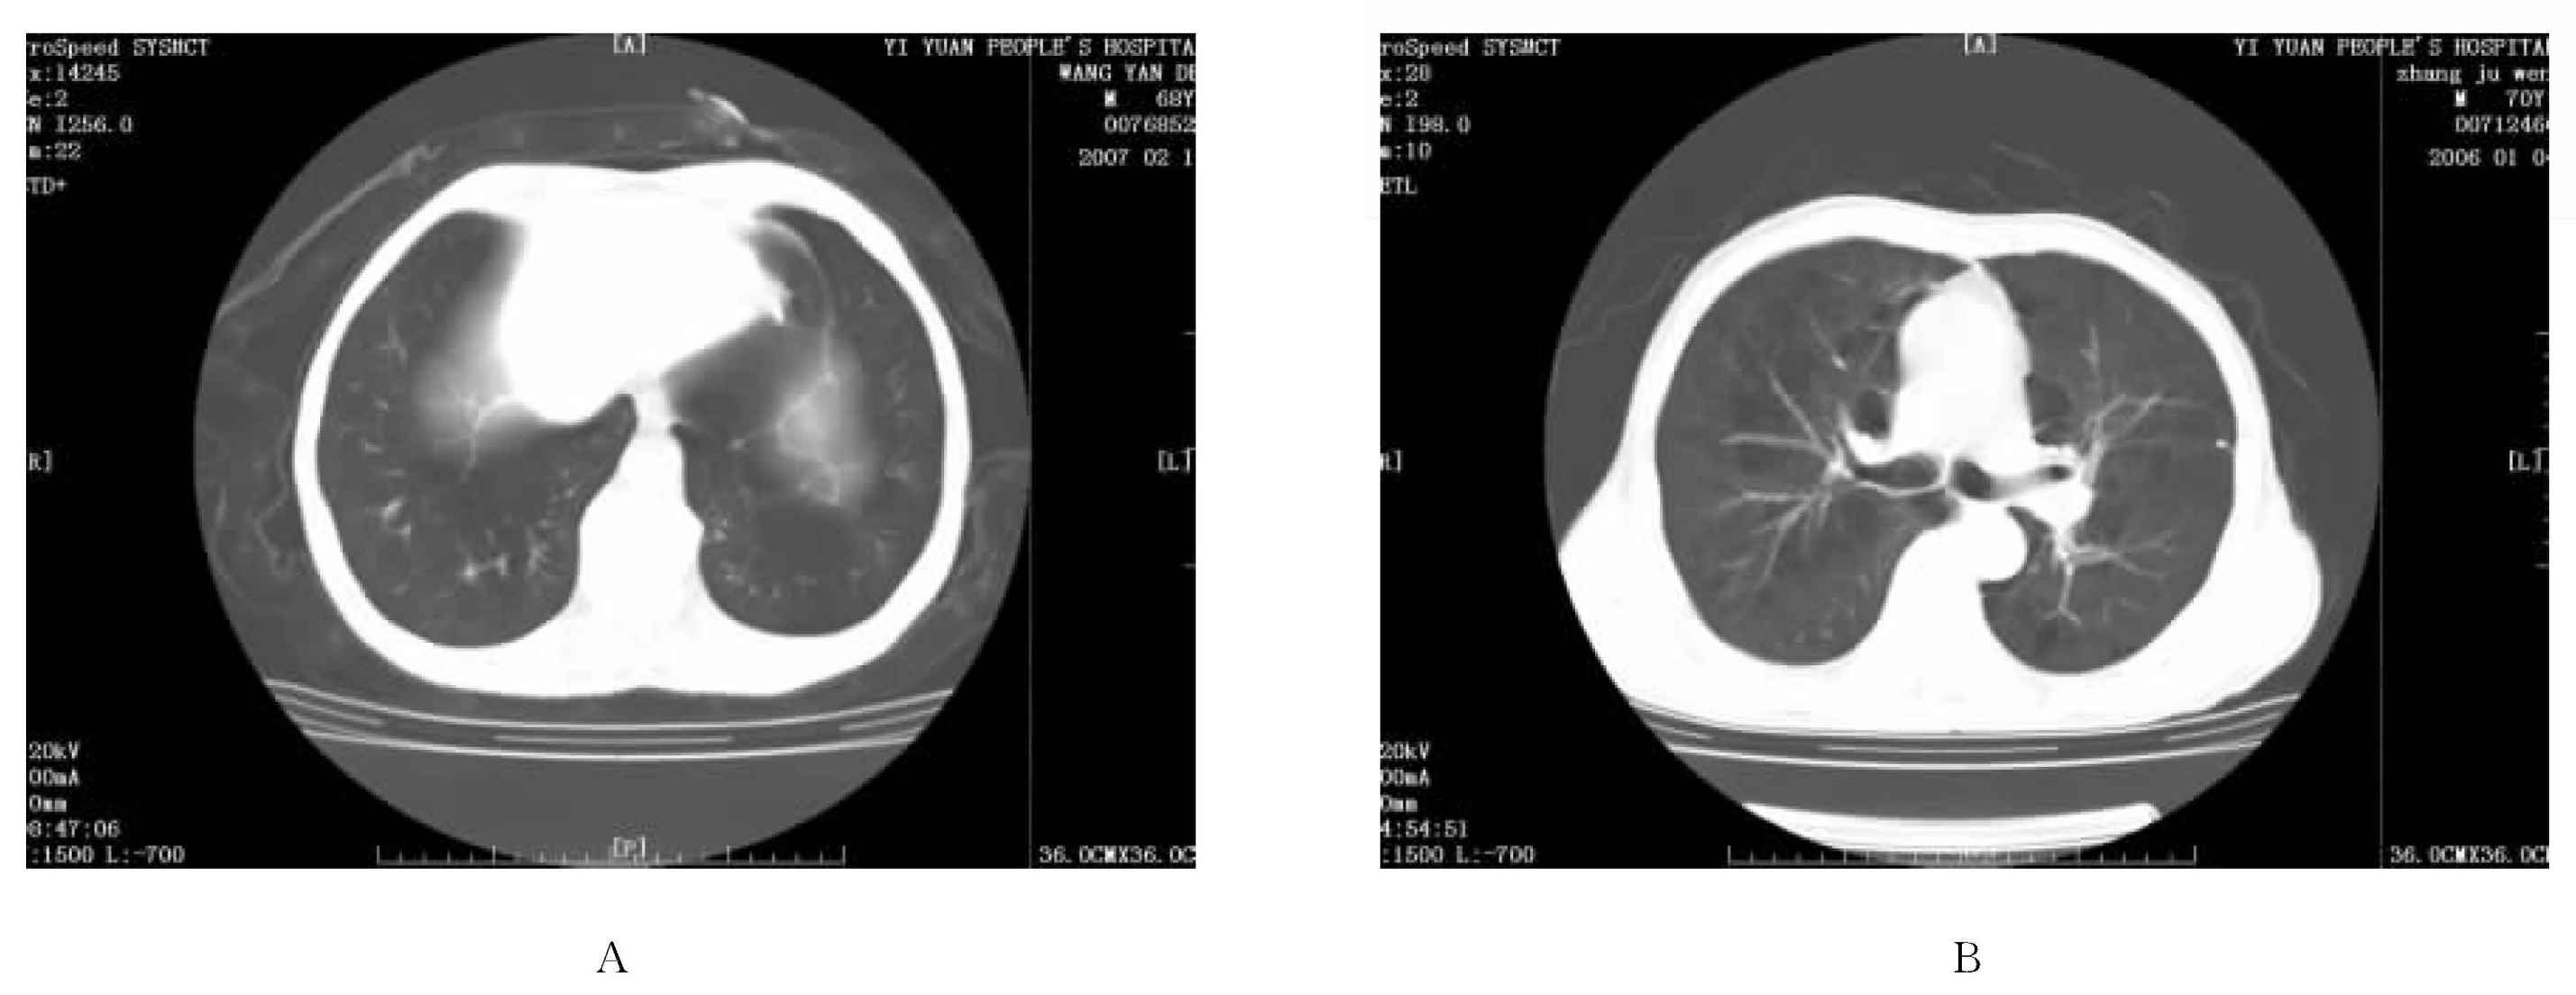
\includegraphics[width=.7\textwidth,height=\textheight,keepaspectratio]{./images/Image00195.jpg}
 \captionsetup{justification=centering}
 \caption{肺气肿\\{\small A.全小叶型肺气肿;B.小叶中心型肺气肿}}
 \label{fig9-11}
  \end{figure} 

此外,应该注意:肺气肿继发感染,炎症区可出现假空洞征和假蜂窝影。

\subsection{肺大泡}

\textbf{【病因病理】}
是因小支气管呈活瓣性阻塞,肺泡过度膨胀、破裂互相合并而成。其直径>1cm。

\textbf{【影像学表现】}
肺大泡呈薄壁环形低密度区,壁薄如线(图\ref{fig9-12})。巨大肺大泡可压迫周围肺组织,使囊壁增厚。肺大泡可单发或多发,大小不一;多位于肺的周边,以肺尖、肺底常见;可有液平面。较小的大泡以CT显示为优。肺大泡即可见于弥漫性肺气肿,亦可见于局限性阻塞性肺气肿。

\begin{figure}[!htbp]
 \centering
 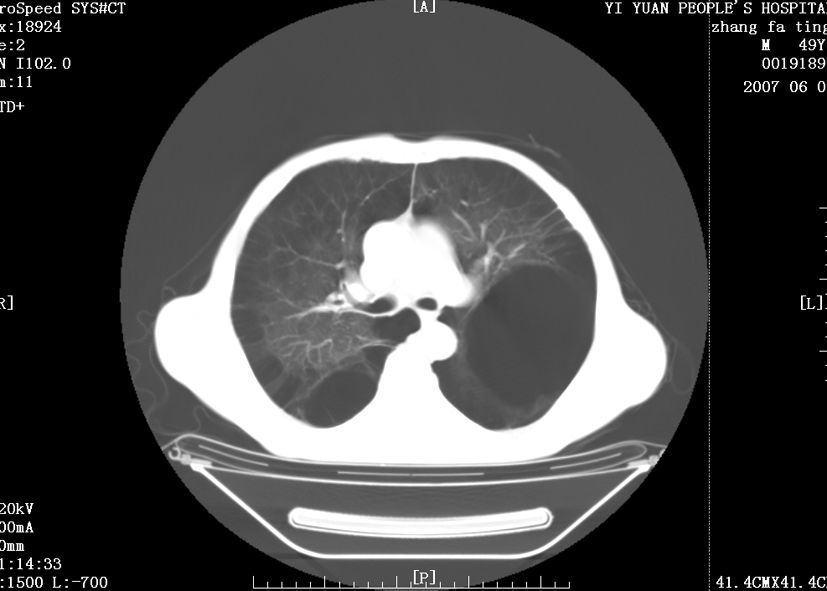
\includegraphics[width=.7\textwidth,height=\textheight,keepaspectratio]{./images/Image00196.jpg}
 \captionsetup{justification=centering}
 \caption{肺大泡\\{\small 双肺部均有多个近圆形低密度区,壁薄如线}}
 \label{fig9-12}
  \end{figure} 

\subsection{特发性肺大泡综合征}

本病又称消失肺综合征。系原因不明的一种大泡性肺气肿,有别于慢性支气管炎、肺结核、尘肺等引起的继发性肺大泡。国外学者Burke于1937年发现这类肺大泡区内肺纹理逐渐消失,首次提出“消失肺”。1987年Roberts等确定了放射诊断标准,即一侧或双侧肺上叶肺大泡至少占据一侧胸腔的1/3以上,正常肺组织受压。

本病的发病机理尚不清楚,可能系肺弹力纤维组织的先天性发育不良或缺乏,导致肺泡壁扩张,形成肺大泡。当大泡胀到一定程度则破裂发生气胸。家族性发病者可能与遗传因素有关。

从上述诊断标准不难看出,该症的肺大泡好发于上肺叶(亦可多在中、上肺),但也有同时分布于下肺野者。

CT平扫尤其HRCT能更全面地观察肺大泡的分布位置、形态、数量及大小,并可显示可能存在的肺气肿及其类型(如间隔旁肺气肿、小叶中心型肺气肿)和少量气胸等。

\subsection{局限性阻塞性肺气肿}

局限性阻塞性肺气肿是由于一个较大的支气管产生部分性阻塞所引起。可见于支气管内异物、小儿急性肺炎、早期支气管肿瘤和支气管慢性炎性狭窄(包括结核等病史)。

\textbf{【影像学表现】}
在影像学上呈局限性密度减低和膨胀区。至于有无胸廓、横膈等改变取决于病变的范围和部位。

\subsection{代偿性肺气肿}

代偿性肺气肿属于局限性非阻塞性肺气肿,是由于一部分肺的纤维化或不张、或手术切除后,其余的肺膨胀代偿其胸腔内失去的体积所致。

\textbf{【影像学表现】}
代偿性肺气肿的范围和程度取决于肺萎缩的程度或肺切除的多少。如果一侧肺完全切除或不张,对侧的肺可全部产生代偿性肺气肿,甚至形成纵膈疝。一叶、一段或少于一叶的代偿性肺气肿较为常见。由于其范围小,一般不产生明显的胸廓、横膈或心脏、纵隔的改变。

\subsection{间隔旁肺气肿}

本病亦有肺小泡之称。肺气肿位于肺小叶的外周部肺泡。病人多无症状,但易发生气胸,而出现相应症状。

\textbf{【CT表现】}
典型者表现为胸膜下局限性低密度区,一般≤1cm(图\ref{fig9-13})。多数病变长轴与胸膜平行,多个间隔旁肺气肿可相互融合,其间有线形的分隔。HRCT有助于显示较小的病灶。常与小叶中心型肺气肿并存。

\begin{figure}[!htbp]
 \centering
 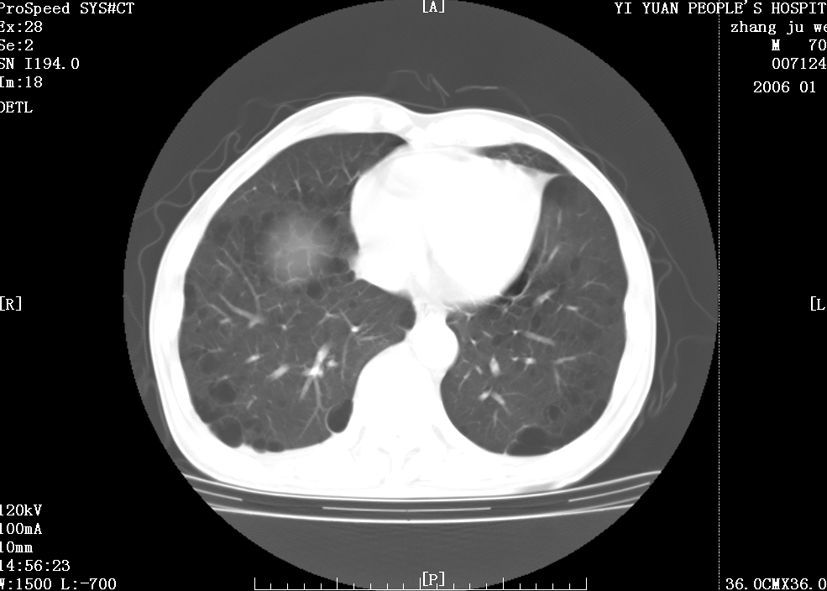
\includegraphics[width=.7\textwidth,height=\textheight,keepaspectratio]{./images/Image00197.jpg}
 \captionsetup{justification=centering}
 \caption{间隔旁肺气肿\\{\small 双侧胸膜下有局限性低密度灶,与小叶中心型肺气肿并存}}
 \label{fig9-13}
  \end{figure} 

\subsection{瘢痕旁肺气肿}

\textbf{【病因病理】}
此型肺气肿为肺脏纤维化瘢痕病变周围的异常的含气腔隙。引起此型肺气肿的纤维化或瘢痕病变常见为肺结核、尘肺进行性块状纤维化等。

\textbf{【CT表现】}
有可见的肺内纤维灶时,识别本型肺气肿较易。可见瘢痕病变周围有片状、不规则含气腔隙,其内无血管、支气管。但当它与仅在显微镜下能见到的肺纤维化共存时,则CT上不能与小叶中心型肺气肿相鉴别。

\subsection{间质性肺气肿}

本病是由于支气管或肺泡破裂后,空气进入间质所引起。随后气体可沿着支气管或血管周围间隙流入纵隔或心包,产生纵隔积气或心包积气,并可到达皮下形成皮下积气。

\textbf{【病因】}
①外伤性:可由于胸部穿刺、胸廓切开以及严重的胸廓外伤所引起。后者以在车祸事故中较多见,不一定伴有肋骨骨折或气胸。②自发性:可随支气管哮喘、百日咳的阵咳或其他原因的支气管刺激而发生。

\textbf{【CT表现】}
支气管、血管周围类圆形的气体影或伴随支气管、血管影的线条状气体影。HRCT可显示小叶细支气管、血管周围的气体影,小叶间隔增宽并见细线状透亮影。还可表现为纵隔积气、皮下积气和心包积气,偶有气腹表现。

\subsection{慢性阻塞性肺病}

慢性支气管炎、支气管哮喘、闭塞性细支气管炎、支气管扩张和肺气肿,总称为慢性阻塞性肺病。

\textbf{【影像学表现】}
慢性阻塞性肺病其低密度的肺气肿内往往可见纤维性改变,网状纤维大而不规则,分布不均匀,以中下肺居多。膈肌位置较老年肺更低平。可见肺动脉增粗、肺心病的表现。

\textbf{【鉴别诊断】}
应注意与老年肺鉴别。老年肺是指发生退行性变的老年人的肺脏。老年肺形态上类似肺气肿的表现,但把它看作肺气肿的一个类型是不合理的。老年肺可见两肺透亮度增强(密度减低)。两肺血管纹理呈细网状,粗细近似、分布均匀。膈肌低平,活动度下降。

\subsection{肺疝}

肺疝是指部分肺组织突出于胸腔范围之外。其分类可根据部位和病因而定。在解剖上可分为颈、肋间(胸)和膈疝。每一类又分为先天性和获得性。获得性肺疝可分为创伤性、自发性和病理性(肿瘤或炎症过程的结果)。

获得性颈疝常见,可见于慢性咳嗽、肺气肿的老年人。此外,创伤、举重或吹奏乐器亦可引起获得性颈疝。对肋间疝CT易于显示,并能确定其大小和范围。膈肺疝罕见。

总之,肺疝不常见,胸内高压或胸壁抵抗力减弱为其常见原因。

\section{肺水肿}

\subsection{概论}

肺水肿是由于液体从毛细血管渗透至肺间质或肺泡所造成的。

肺水肿根据病因可分为心源性和非心源性。其形成因素主要有两个:①毛细血管压力的改变;②毛细血管通透性的改变。

毛细血管压力增高是肺水肿的最常见原因,大多随着左心疾患时肺静脉血流阻力增高而产生。左心衰竭是引起肺水肿的主要病因,但如右心亦发生衰竭则肺水肿可以减退或消失。

毛细血管通透性改变大多由于血管壁层受损引起。产生这种改变的因素有两类:①体内因素:可为低血氧、贫血、低蛋白血症,亦可由肾脏疾病、急性风湿热和菌血症等所产生的毒素,以及对某些药物的过敏反应等引起。②体外因素:包括各种吸入性病变,如吸入各种毒气和吸入酸性胃液等。

此外,淋巴回流障碍亦可促成肺水肿的产生,但一般不是引起肺水肿的单独因素。

在临床上,肺水肿最常见于心脏病患者,另有一部分见于肾脏病、肝病患者。急性肺水肿偶可见于中枢神经系统疾病,特别是伴有颅内高压时产生,其原理尚不清楚。急性肺水肿还可见于少数新近到高原的人中发生。

\subsection{间质性肺水肿}

\textbf{【病因病理】}
多见于心脏病患者,一般多随着慢性肺淤血的发展而产生,故两者之间不易划清界限。是由于左心衰竭所引起的肺静脉和毛细血管高压的一种征象。由毛细血管渗出到肺组织的液体首先出现于间质部分。

\textbf{【临床表现】}
临床上慢性间质性肺水肿的症状有较大的差异。在轻度的左心功能代偿失调时,可无明显症状。即使有些患者有气急、咳嗽、痰中带血、端坐呼吸等症状时,听诊可为阴性。其诊断以影像学为准。

\textbf{【CT表现】}
肺血管周围的渗出液表现为肺门及肺内血管影增粗、模糊,以中内带为主。小叶间隔中的积液可使其增厚。小叶间隔增厚可作为间质性肺水肿的诊断依据,以及与慢性肺淤血的鉴别依据。

间质性肺水肿以慢性左心衰竭患者最多见,故这类病例中还可见到心影增大、胸腔内少量积液、肺静脉高压征象。

\subsection{肺泡性肺水肿}

其病因较多,诊断较为困难。在一些患者特别是心脏病患者,可与间质性肺水肿并存,但多被肺泡性肺水肿所掩盖。

\textbf{【病理】}
肺泡性肺水肿使肺的体积增大变实。由左心衰竭引起者,水肿以两肺下部和后部为著。在单纯的肺水肿中液体呈白色;如有溢血存在,液体呈红色或棕色。

\textbf{【临床表现】}
急性肺泡性肺水肿的典型表现为严重的气急、端坐呼吸和水泡样啰音。一般伴有咳嗽并有大量的泡沫痰或淡血样痰,并伴有其他心衰表现。慢性肺泡性肺水肿的临床症状差异较大,有些水肿广泛,但症状和体征不明显。

\textbf{【CT表现】}

1.中央型肺水肿:其片状高密度影较对称的分布于两肺野。其密度以肺门区为最高,向外逐渐变淡。肺野外缘宽约2.0~3.0cm的外带、肺尖和肺底,甚至叶间裂旁和纵隔旁可保持清晰。这种分布形态常被称作蝴蝶状,是肺泡性肺水肿的典型表现,但并不多见。本型可为急性或慢性。

2.弥漫型肺水肿:一般表现为散布于两肺的大小不一、密度不等、轮廓不清楚的片状高密度影。以融合在一起的较大斑片状改变较为常见。分布不甚对称,以肺野内中带为主(图\ref{fig9-14})。

\begin{figure}[!htbp]
 \centering
 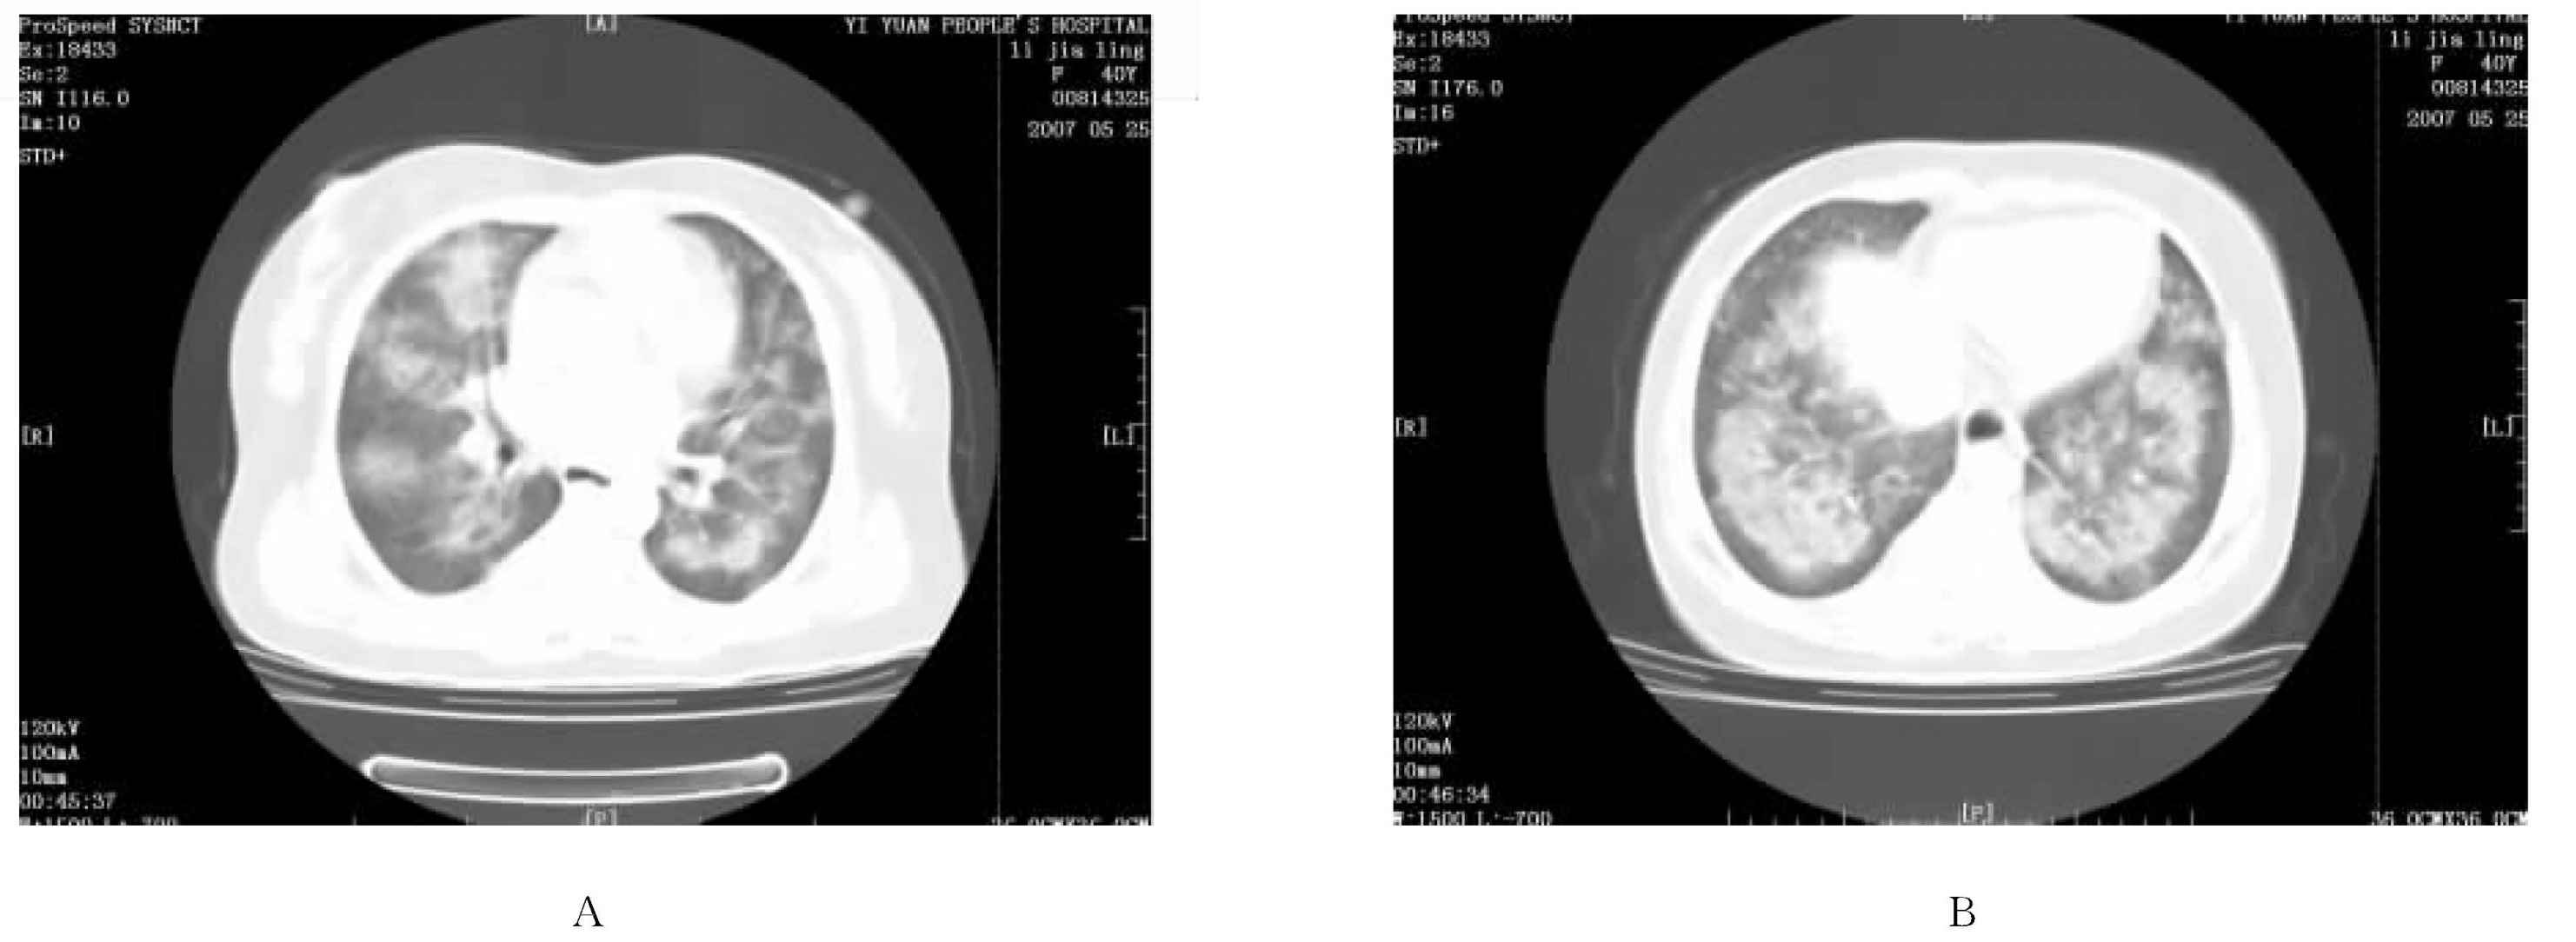
\includegraphics[width=.7\textwidth,height=\textheight,keepaspectratio]{./images/Image00198.jpg}
 \captionsetup{justification=centering}
 \caption{肺水肿\\{\small 两肺的大小不一、密度不等、轮廓不清楚的片状高密度灶}}
 \label{fig9-14}
  \end{figure} 

3.局限性肺水肿:可局限于一叶,或主要见于一侧、两上或两下肺。有时可呈一个或几个孤立的、较大的、轮廓清楚的圆形高密度影,形似肿瘤。

\textbf{【鉴别诊断】}
间质性肺水肿有较特异的小叶间隔增厚,诊断较易;而泡性肺水肿表现复杂,对于分布和形态不典型的病例诊断困难。首先应详细的参阅病史,特别是心血管、肾脏、中枢神经系统疾病,大量补液和吸入毒性气体等病史。

肺泡性肺水肿应注意与融合性支气管肺炎和肺梗死鉴别。临床上如有发热和白细胞增多应考虑为支气管肺炎;如有胸膜性胸痛就必须考虑有肺栓塞可能。但心衰所引起的肺水肿可与支气管肺炎和肺梗死并存,尤其合并肺炎者常见,需动态观察诊断。

\subsection{高原性肺水肿}

本病是一种严重危害生命的急性高原病。常发生在初入或再入高原者,多见于海拔3000m以上的地区。

\textbf{【发病机理】}
目前认为有:①肺动脉高压:当机体处于急性低氧环境下,会立即产生应激反应,短时间缺氧会直接通过神经反射引起收缩,导致肺动脉高压。②毛细血管应激衰竭:国外有学者从本病患者的肺抽取液中发现了不同于心源性肺水肿的高分子蛋白、红细胞和炎性物质,认为本病是毛细血管应激衰竭导致血管壁超微结构损伤所致。③细胞因子作用:近年来从本病患者的肺抽取液中发现除含有大量高分子蛋白、红细胞和炎性物质外,还可见LgM、LgG、补体C3、C4、组织胺等物质。认为本病是一种高蛋白、高渗出性肺水肿,其发生与肺循环中漏孔出现和缺氧所致的体液免疫反应有关。而肺动脉高压在其发生中可能仅起辅助作用。④诱因和易感性:患者绝大多数病前均有劳累、受寒和呼吸道感染等诱因。

\textbf{【临床表现】}
国内1组报道,男多于女,年龄19~54岁,中位年龄35.5岁。本病发病急、进展快、危害严重。表现为严重的气急、端坐呼吸和水泡样啰音。可伴有咳嗽并有大量的泡沫痰或淡血样痰。

\textbf{【CT表现】}
亦可分为肺泡性(包括中央型、局限型和弥漫型)和间质性肺水肿,后者相对少见。早期和恢复期主要表现为间质异常;进展期与稳定期以肺实质病变为主,且在未实变区常可见明显的代偿性肺气肿。总之,高原性肺水肿早期呈磨玻璃密度,多出现于下叶上段及后底段,且右下叶早于左下叶;中期为云絮状密度增高,并发进一步展到上叶后段及前段,病变充满整个肺叶,且右肺重于左肺;恢复期表现为实变区从实变到磨玻璃改变过渡到正常。

\subsection{复张性肺水肿}

本病是指胸腔积液或积气,经抽液或抽气后,复张肺组织内产生的肺水肿。

\textbf{【病因病理】}
复张性肺水肿的发生可能为多种因素作用的结果,其中肺泡表面活性物质的缺乏是重要的原因。当肺萎缩时,肺血管收缩痉挛,肺血流量减少,从而影响肺泡Ⅱ型细胞的代谢,造成肺泡表面活性物质的分泌减少,使肺泡表面张力增高。复张时,增高的肺泡张力导致肺毛细血管周围产生负压。当此压力与肺毛细血管压力之和大于血浆胶体渗透压时,就使血管内液体外渗引起肺水肿。

在其发生过程中,机体缺氧所致的毛细血管通透性增高、肺萎缩时静脉和淋巴回流的阻滞、复张时肺血流量的增加亦为重要的协同因素。而胸腔内压的突然下降则是复张性肺水肿的主要诱因。

\textbf{【影像学表现】}
呈单侧弥漫性或局限性肺泡性肺水肿,亦可伴有间质性肺水肿征象。

\subsection{成人呼吸窘迫综合征}

本症是毛细血管通透性增加引起的非心源性肺水肿,包括不同原因(如休克、创伤、严重感染)引起的具有特征性临床、病理和影像学表现的呼吸衰竭。其本质可能是肺急性循环障碍(微血管痉挛、栓塞、通透性增强)。其三联征即低氧血症、肺顺应性减低以及肺浸润已被充分认识。此症命名很多,如急性肺损伤综合征、成人肺透明膜病、成人呼吸功能不全综合征、毛细血管漏综合征、急性肺不张、脂肪栓塞综合征、出血性肺不张、出血肺综合征、非心源性肺水肿、外伤后肺不张、进行性肺实变、进行性呼吸窘迫、肺微血栓综合征、休克肺、僵肺综合征、创伤性湿肺、白肺综合征等。

\textbf{【病因】}
常见的基础疾病有:严重感染、脓毒症、误吸、严重创伤、多发骨折、大手术、烧伤、头部创伤、肺挫伤、休克输血输液过量、败血症、DIC、胰腺炎、吸入烟雾和有毒气体、氧中毒、淹溺、羊水栓塞、脂肪栓塞、低血压、低蛋白血症、应用大量激素后突然停止或减量太多等。

\textbf{【临床表现】}
在原发疾病的基础上急性发病。病人有呼吸困难、干咳、烦躁不安、发绀。肺毛细血管压正常、肺顺应性降低,正常压力及高浓度给氧时,患者仍有严重低氧血症。

\textbf{【影像学表现】}
分4个阶段。①正常;②间质性肺水肿;③泡性肺水肿;④病变吸收或残留纤维化。

CT可发现气压伤合并症如肺气囊、气胸、纵隔积气;也可发现感染合并症如肺脓肿、脓胸。

\section{肺栓塞和肺梗死}

\subsection{概述}

肺栓塞又称肺动脉栓塞。是指内源性或外源性栓子栓塞肺动脉或其分支,引起肺循环障碍的临床和病理生理综合征。

\textbf{【病因】}
大多由于周围静脉内血栓脱落后随血循环进入肺动脉引起。血栓的发源部位最常见于下肢和盆腔静脉(约90%以上来源于下肢深静脉),其次为上肢及颈部静脉;在有些心脏病患者中,血栓可产生于左心房或右心室;亦可为脓毒栓子或继发于肺内疾病如曲菌病和肿瘤。

\textbf{【病理】}
其病理过程为静脉血栓形成、血栓栓子脱落栓塞肺动脉及栓塞后期3个阶段。肺动脉栓塞在肺内所产生的病理生理演变和临床症状取决于下列因素:①有无心脏、肺部疾病存在;②栓子的大小、数目和部位;③血栓栓塞为部分性或完全性。因肺组织为双重供血,故梗死发生率为10%~30%。肺段动脉的栓塞一般不引起肺梗死,因为完善的支气管动脉循环足够维持肺栓塞区的血供。有时可因血液外渗和水肿液充填肺泡而实变,可于3~10天内完全吸收,不残留纤维化改变。梗死一般发生于心肺疾患而致血液淤滞者,大多涉及肺段,可多发,偶可累及整个肺叶。肺梗死吸收慢,常残留瘢痕。

\textbf{【临床表现】}
大多不产生临床症状,或者仅产生轻微不适。一个大的肺动脉栓塞可导致突然死亡,如不死亡可产生典型的休克症状。当栓塞并有肺梗死时,可产生气急、呼吸困难和持续加重的脉搏增速现象,并可产生发热、胸膜性胸痛、咳嗽和咯血等症状。其中以气急和胸痛加重为常见,咯血较少见。典型的气急、胸痛和咯血三联征仅存在于20%左右的病例。

其CT表现见下述。

\subsection{肺栓塞}

肺动脉栓塞多发生在叶、段肺动脉及其以下分支,累及主肺动脉和左、右肺动脉较为少见。肺动脉内栓子的直接显示是诊断肺栓塞的最可靠的直接征象。

\textbf{【CT表现】}

1.直接征象:增强扫描肺动脉腔内的半月形或环形(附壁血栓)充盈缺损、完全梗阻及双轨道征为其直接征象。①部分性血栓栓塞:即血栓部分阻塞肺动脉。急性期栓子游离于血管腔内,在与扫描层面垂直时呈圆形低密度,周围环以高密度造影剂;如与扫描层面平行则中央的栓子呈条状低密度带,两边的造影剂呈与之平行的高密度,称为“双轨征”。慢性期血栓收缩趋向不规则,并与血管壁粘连,CT表现血栓呈偏心性、与管壁呈钝角相交。故“双轨征”提示为急性肺栓塞,动态观察还可见栓子在腔内活动。但这种急、慢性的区别是相对的,有时是不可能的。②完全性血栓栓塞:即血栓基本上完全阻塞肺动脉(图\ref{fig9-15}A、B)。有学者认为伴受累肺动脉增粗提示为急性,伴受累肺动脉细小提示为慢性血栓。③环状附壁血栓:一般认为是血栓溶解再通所致,当然尚难完全排除原发于肺动脉的血栓形成。

2.间接征象:①肺少血征:肺纹理纤细、缺失。②马赛克征:在肺窗上部分病例可见该征。是由于肺灌注的区域性不均匀,导致在吸气HRCT上可见的肺衰减差异,反映血管阻塞或通气异常。该征更多见于气道疾病。表现为以肺叶、段或亚段为单位的肺组织透亮度增加与邻近灌注正常或轻度灌注增加的肺组织形成“马赛克样”表现。③肺实质密度增高:尤其是楔形的以胸膜面为底的实变,常伴胸膜反应(图\ref{fig9-15}C、D)。④其他:右心室肥厚、右心室功能下降、肺动脉扩张、支气管动脉扩张(管径>1.5mm)、心包积液等;气胸偶见,机制不明。⑤此外,平扫时可见因血栓机化(多在数天及数周内机化)所致的局限性密度增高;或因血栓时间短、含水分多,而显示肺动脉局限性密度减低。

\begin{figure}[!htbp]
 \centering
 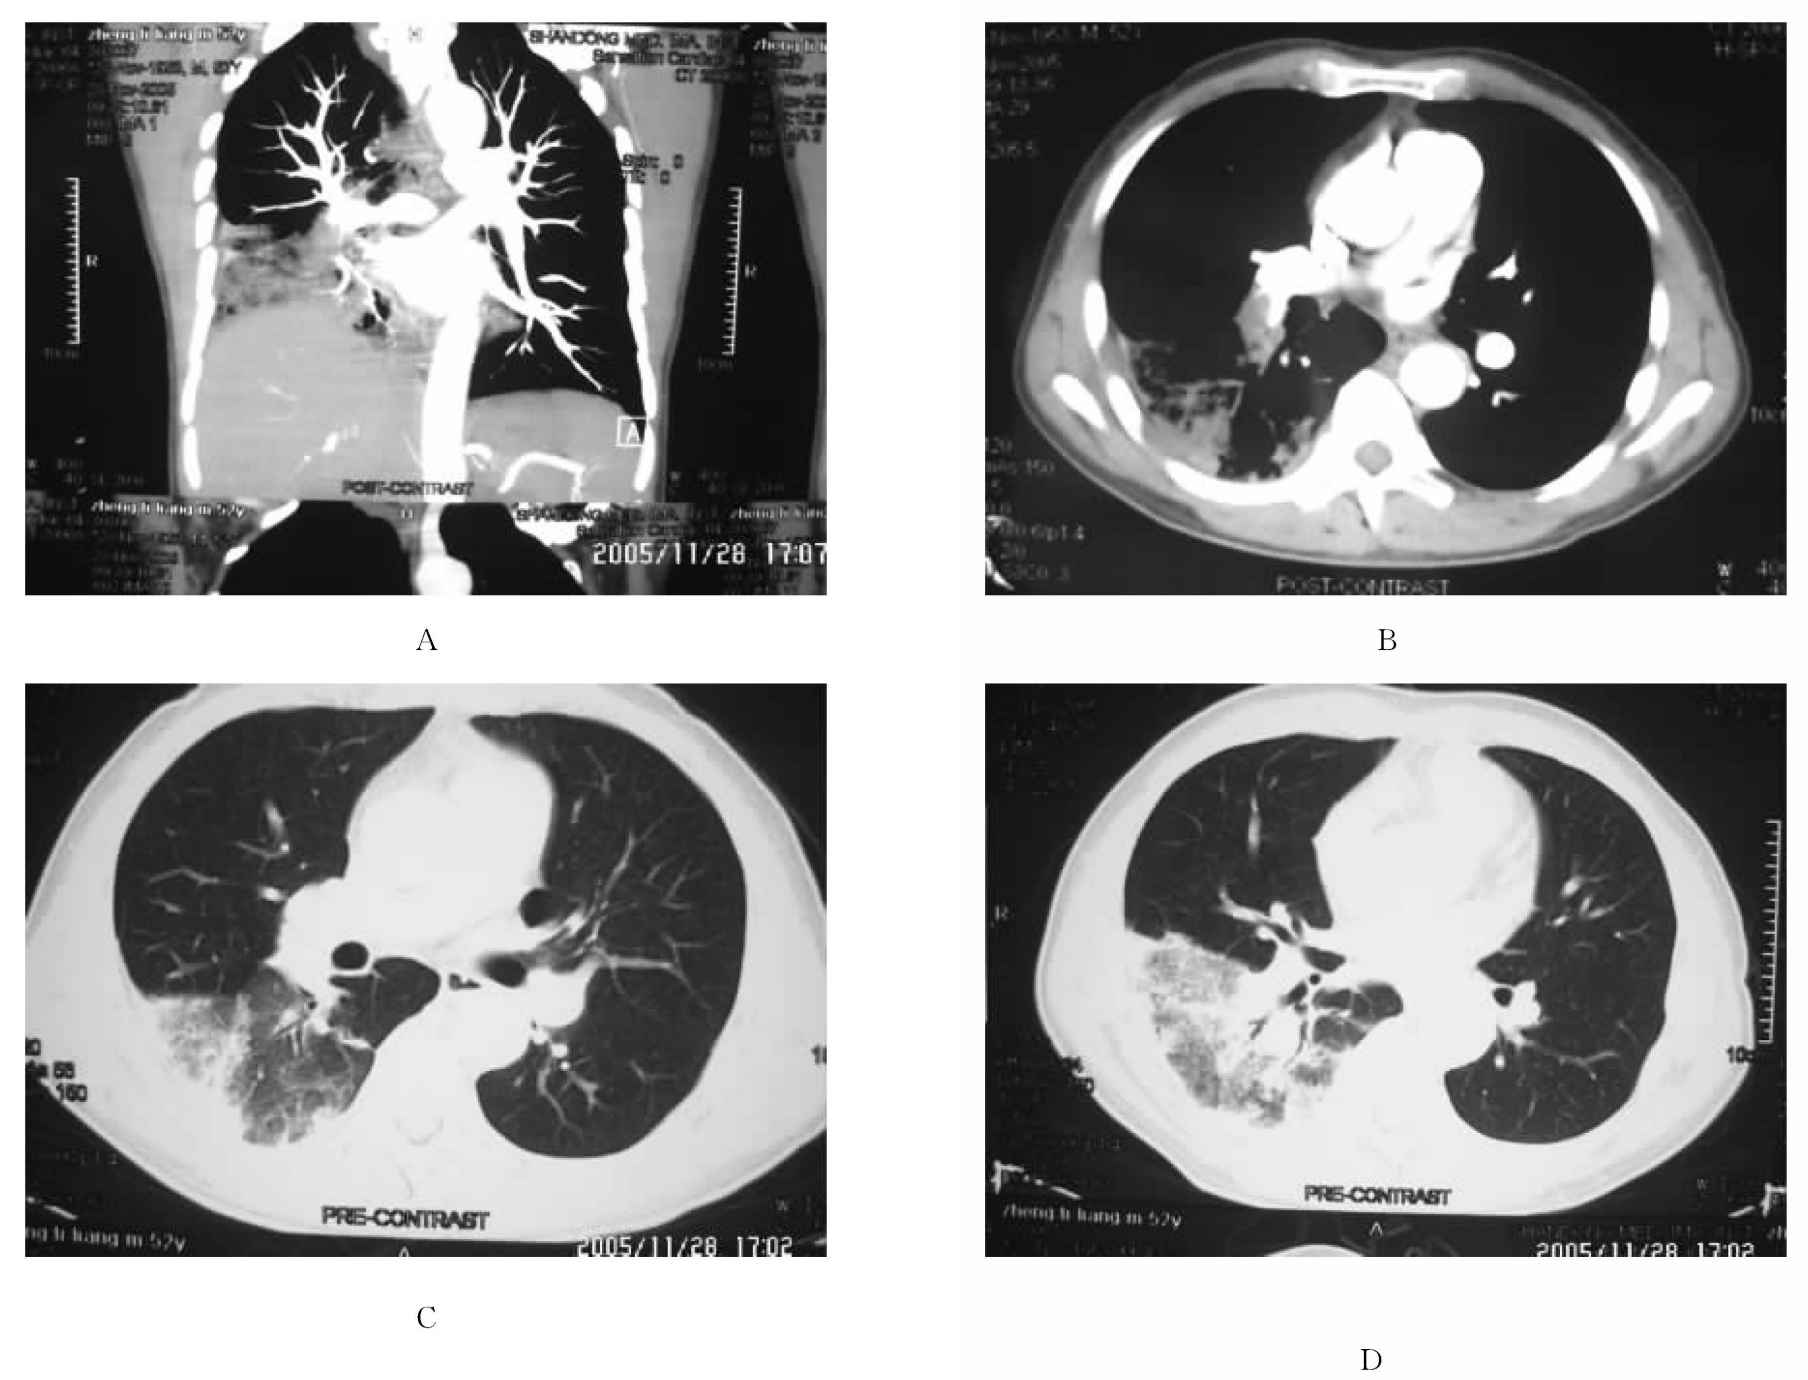
\includegraphics[width=.7\textwidth,height=\textheight,keepaspectratio]{./images/Image00199.jpg}
 \captionsetup{justification=centering}
 \caption{肺动脉栓塞\\{\small A~D为同一患者,右下肺动脉基本完全阻塞,右下肺实变}}
 \label{fig9-15}
  \end{figure} 

\subsection{肺梗死}

分析肺梗死时应注意阴影的形状、大小、位置、密度、边缘、有无胸膜反应。

\textbf{【CT表现】}
其典型表现见于肺段性梗死,显示为一个均匀的楔状或锥形高密度影,位于肺野外围,基底与胸膜面邻接,顶部指向肺门,边缘较平整清楚。总之,其表现有:①三角形的特点,占40%,也可呈圆形、椭圆形、梨形和不规则形;②病灶比大叶小、比小叶大者居多;③右肺比左肺多,下比上多;多为单发,也可多发;④密度多均匀,边缘清晰,病灶内可见网格、含气支气管征、小空洞征等;⑤可有胸膜反应,有少量或中量积液;⑥梗死病灶一般2~3周吸收,短者2~3天,长者4~5周;吸收时体积向心性缩小,呈“溶冰征”有一定特异性;⑦条状阴影为盘状不张、坏死形成的肺实质瘢痕,以及梗死表面的胸膜或叶间胸膜增厚所引起。

\textbf{【鉴别诊断】}
许多学者指出,肺栓塞亦可出现密度增高区,且并不代表急性梗死或肺组织的坏死。实验证实其影像学所见到的实变阴影可以是水肿、出血或肺不张。导致肺不张的机理可能两种:一是肺泡区的血流被栓子阻塞后大量的肺泡死腔增加,从而促使肺收缩;二是血流量减少,表面活性物质的分泌减少,引起粘连性肺不张。肺梗死形成的实变区有水肿、出血、坏死组织,当然也有不张的因素。但只有实变区出现空洞或实变区消失后留有瘢痕或结节时,才能诊为梗死。

总之,无论伴有或不伴有梗死,实变区可由水肿、出血和不张所造成。尚无影像学标准区分是栓塞或梗死,诊断梗死者需有上述特殊征象出现。

事实上,除直接征象血栓和早期局部密度减低、肺纹理纤细、缺失外,上述表现和演变过程亦可见于感染性肺病,所以需密切结合临床症状和实验室检查确诊。但国外有学者认为肺梗死灶吸收时体积向心性缩小呈“溶冰征”,与急性肺炎不均匀吸收不同,具有特异性。

\section{肺部炎症}

\subsection{概述}

\subsubsection{分类}

1.按病因学分类
①感染性:最常见。包括细菌、病毒、真菌、支原体、立克次体、衣原体、钩端螺旋体和寄生虫感染等。②理化性:包括毒气、毒物、药物和放射线等。③免疫和变态反应性:包括过敏性和风湿热等。

2.按解剖学分类
①大叶性:是指炎症累及整个肺叶或多个整肺叶,也称为肺泡性肺炎。②小叶性:是指炎症累及细支气管、终末细支气管及其远端的肺泡,常为两侧小片分布,有融合趋向,也称为支气管肺炎。③间质性:是指炎症主要累及肺的间质。

\subsubsection{}

\begin{table}[htbp]
\centering
\caption{几种肺炎的病理及影像学表现}
\label{tab9-4}
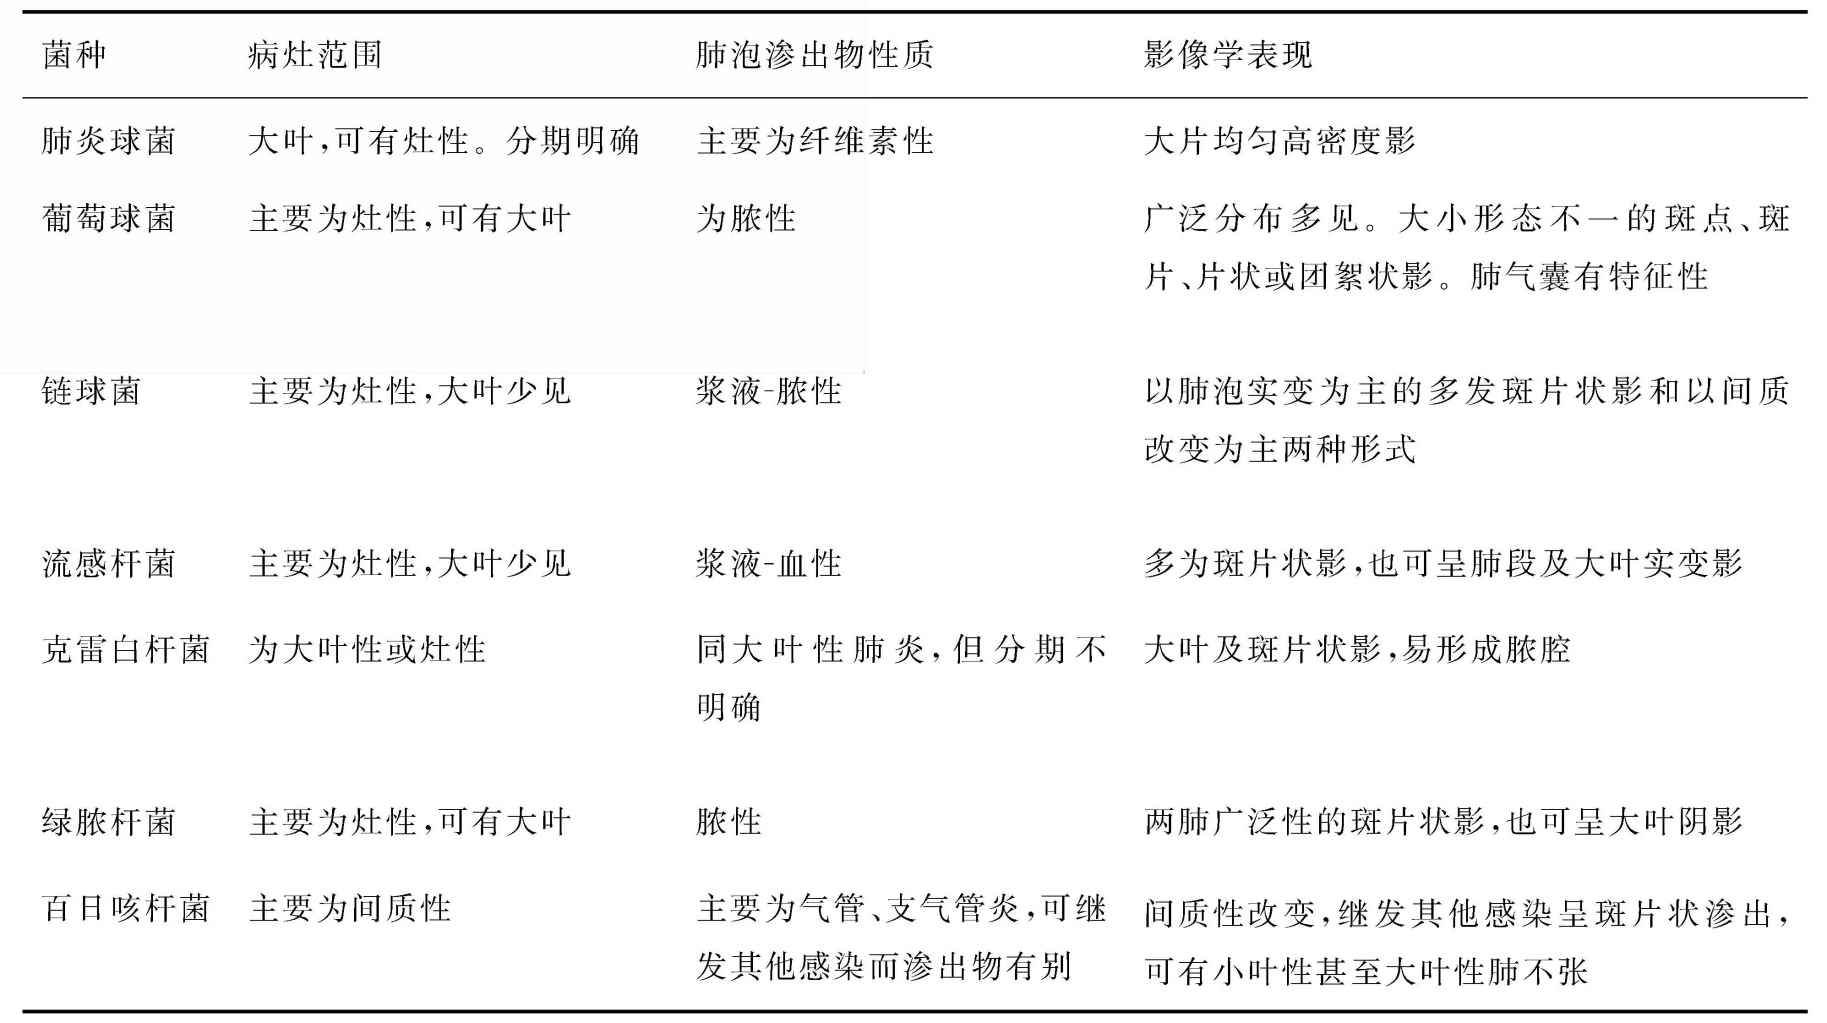
\includegraphics[width=\textwidth,height=\textheight,keepaspectratio]{./images/Image00200.jpg}
\end{table}

\subsubsection{肺炎比较特殊的影像学表现}

肺炎的病灶分布和形态受支气管-肺泡系解剖特征的影响。此外,还应考虑病源和机体反应因素,使肺炎的影像学表现复杂化、特殊化。肺炎比较特殊的影像学表现为:①肺水肿样表现;②包裹性胸膜炎样表现,但边缘模糊;③单发或多发的大团块状病灶;④一侧肺多叶实变;⑤粟粒或结节病灶表现。

\subsubsection{慢性肺炎、机化性肺炎和肺炎性假瘤的内在联系}

目前认为3者均为肺炎转归期的表现,从病理上讲3者是不易区分的。并有人认为机化性肺炎是慢性肺炎的一种类型,甚至认为球形肺炎是慢性肺炎的一种特殊形态表现。亦有人将肺炎不完全吸收或延迟至4~8周后吸收的肺炎称为机化性肺炎。慢性肺炎和机化性肺炎均有局限性和弥漫性、实质性和间质性之分。但影像学多将局限性慢性肺炎、局限性机化性肺炎和炎性假瘤作为慢性炎块进行集中研究。可是无论从影像上还是临床上,似乎区别局限性慢性肺炎和局限性机化性肺炎都是困难的。有人认为局限性机化性肺炎是不可逆的、不需治疗的,但多数学者认为进行抗炎治疗后,病变范围可以缩小甚至完全消失。国外有学者建议对可疑局限性机化性肺炎抗炎治疗、动态观察1个月以利于确诊,局限性慢性肺炎抗炎治疗多是有效的。同样急性肺炎也可呈结节状或肿瘤形状,但抗炎治疗后2~4周吸收,而炎性假瘤经3个月或更长时间无变化。

\subsection{大叶性肺炎}

\textbf{【病因病理】}
大叶性肺炎最常见的致病菌是肺炎双球菌。克雷白杆菌亦可呈大叶性实变,但病情较重,由于渗出物比重高,最易使肺叶膨胀并产生组织坏死和空洞。此外,链球菌、流感嗜血杆菌、绿脓杆菌和大肠杆菌偶可呈大叶性。大叶性肺炎是由小的感染性颗粒作为病源被吸入到肺的外周,并在该处引起反应灶。起初组织反应渗出液进入肺泡间隙,继而进入气道及肺泡。当肺泡充盈后,渗出液通过肺泡孔和Lamber小道播散到邻近肺小叶及肺段,并不经支气管血管束或肺间质播散。病变不经细支气管播散,故大叶性肺炎常不随肺段分布。更确切地说,在病程早期,大叶性肺炎所产生的阴影似乎侵及多个肺段。诚然,由于肺炎的早期诊断和抗菌药的治疗,常使病变早期得到控制。所以,典型的大叶实变较少遇到。同样,把肺段性实变认为是大叶性肺炎的表现形式亦是错误的。

病理分期:大叶性肺炎典型变化分为4期:①充血期:发病后12~24小时;②红色肝样变期:发病后2~3天;③灰色肝样变期:发病后4~6天;④吸收消散期:发病后7~10天。

\textbf{【临床表现】}
多在发病前有受凉、过度劳累或上呼吸道感染。起病急骤,先有寒颤高热、胸痛,痰较黏厚或有典型的铁锈色痰。下叶肺炎刺激膈胸膜导致的疼痛可放射到上腹痛。实变期局部叩诊出现浊音、语颤增强、呼吸音减低和啰音等。

\textbf{【CT表现】}
①充血期:X线平片通常不易发现,CT表现为磨玻璃样高密度影,界限不清。②实变期:表现为呈大叶性或肺段性分布的高密度实变区。其内肺纹理消失,可见支气管充气征(图\ref{fig9-16})。炎症实变的肺叶体积一般与正常时一致。③消散期:病变吸收,实变区密度逐渐减低,呈散在的、大小不一的和分布不规则的斑片状高密度灶。进一步吸收病变区仅留下少许条索状高密度灶,最后多恢复正常。在少数病例,特别是老年患者,全部吸收可延迟到3个月或更长时间,甚至演变为机化性肺炎。

\begin{figure}[!htbp]
 \centering
 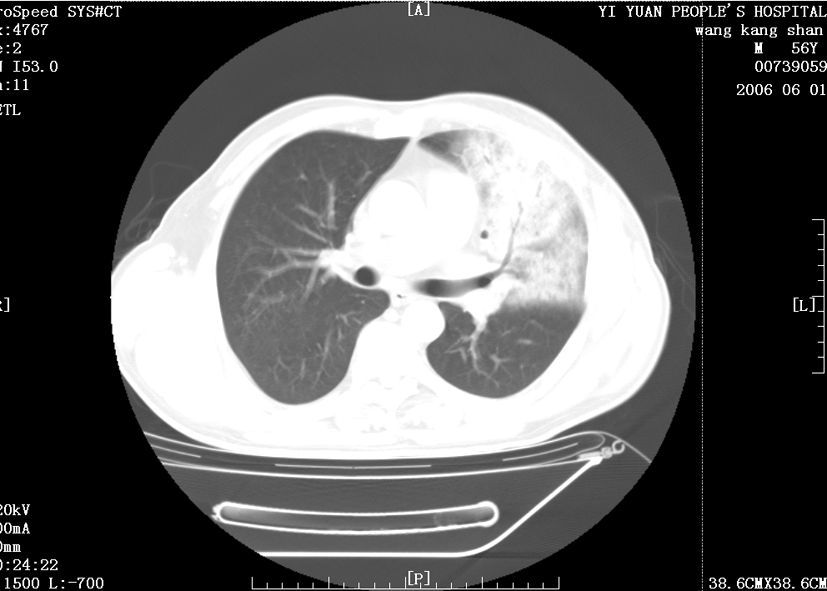
\includegraphics[width=.7\textwidth,height=\textheight,keepaspectratio]{./images/Image00201.jpg}
 \captionsetup{justification=centering}
 \caption{大叶性肺炎\\{\small 左上叶密实、密度均匀,以斜裂为界;可见支气管充气征}}
 \label{fig9-16}
  \end{figure} 

\textbf{【鉴别诊断】}

1.支气管肺炎:①大叶性肺炎充血期表现为磨玻璃样高密度影。而支气管肺炎早期呈较弥漫的支气管炎、支气管周围浸润征象,HRCT呈“树枝发芽征”。②大叶性肺炎于实变期呈均匀的密度增高影,无多灶性分布的特点。如呈大叶性,将呈现其相应形态,可有空气支气管征。肺叶体积一般变化不大。而支气管肺炎呈多灶性、界限不清的腺泡结节状或小片状实变影,可融合成片,但仍有多灶性征象。③大叶性肺炎的吸收消散期,可呈散在的、大小不一的和分布不规则的斑片状甚至条索状阴影,其后逐渐恢复正常。在少数病例可演变为机化性肺炎。而支气管肺炎的吸收一般不遗留下条索状影,但融合成片者亦可演变为机化性肺炎。

2.大叶性肺不张:亦可呈大叶性实变,但肺容积缩小、叶间裂凹陷,邻近组织器官向病变区移位。

3.干酪性肺炎:多见于右上叶,其实变为多中心性团絮状干酪灶的融合。其密度较大叶性肺炎高,但不均匀,其中见不规则空洞。邻近肺组织内常有支气管播散灶。结合临床可予以鉴别。

此外,大叶性肺炎甚至支气管肺炎,在吸收过程中密度不均,但密度较结核低,无增殖性、干酪性病灶表现;肺炎吸收时有纤维化表现,但无结核各种病灶混杂的特点。尽管如此,大叶性肺炎消散期、结核、支气管肺炎三者的鉴别仍可能有困难。

\subsection{支气管肺炎}

本病亦称为小叶性肺炎。主要发生于婴幼儿、青少年和老年体弱者。

\textbf{【病因病理】}
常见的致病菌为肺炎双球菌、金黄色葡萄球菌、链球菌及嗜血性流感杆菌。此外,亦可为病毒和支原体引起。本病常为麻疹、百日咳、流感后的并发症。支气管肺炎的主要受损部位是在终末及呼吸性细支气管。本病以急性支气管炎或细支气管炎开始。如毒性较剧的金黄色葡萄球菌和变形杆菌等,则坏死性支气管和细支气管炎能导致肺小动脉的栓塞。这些炎症反应经过细支气管壁而侵犯肺泡壁,随之而来的渗出液和炎性细胞进入肺泡造成小叶实变。肺泡内充满水肿液、血、多形核白细胞、透明膜和细菌。易致细支气管不同程度的阻塞,可出现小叶性肺气肿或肺不张。坠积性肺炎与患者的习惯性卧床体位有关。

\textbf{【临床表现】}
发病急骤,有寒颤高热、咳嗽,咳稀薄粉色痰、脓性痰或血性痰,常有胸痛、呼吸困难。体检无明显实变,双肺有啰音。

\textbf{【CT表现】}
早期呈较弥漫的支气管炎、支气管周围浸润征象,HRCT呈1~5mm的小叶中心结节状和短线状影像并与支气管血管束相连,即小气道结节之“树枝发芽征”。小叶实变后呈多灶性、界限不清的腺泡结节状或小片状实变影,可融合成片,但仍有多灶性征象(图\ref{fig9-17})。支气管肺炎的吸收一般不遗留下条索状影,但久不消散的支气管肺炎可引起支气管扩张,融合成片者可演变为机化性肺炎。

\begin{figure}[!htbp]
 \centering
 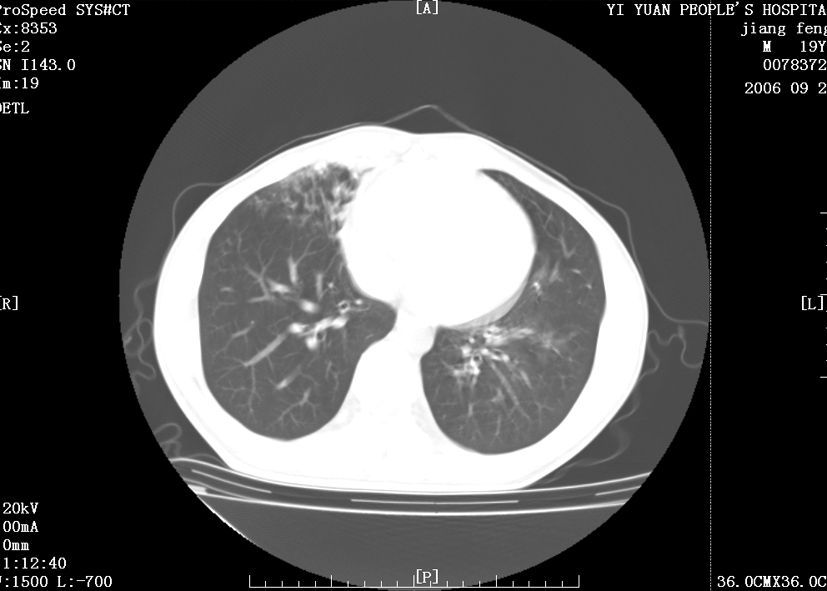
\includegraphics[width=.7\textwidth,height=\textheight,keepaspectratio]{./images/Image00202.jpg}
 \captionsetup{justification=centering}
 \caption{支气管肺炎\\{\small 右中叶有许多斑片状高密度灶}}
 \label{fig9-17}
  \end{figure} 

美国著名的放射学家James.C.Reed认为:支气管肺炎常累及支气管和细支气管,所以偶可同时有支气管狭窄和黏液栓而导致气管阻塞。与大叶性肺炎相比,大叶性肺炎的阴影常呈非节段性分布,且很少出现肺不张。而支气管肺炎的阴影反而常呈节段性或大叶性分布,当然病灶形态仍不失多灶性的特点(并非多发病灶)。支气管肺炎仅局限于叶或段,随之而来的肺容积减少较常见,具有这种表现的支气管肺炎有时被称为不张性肺炎。如在其他肺叶也有多灶性阴影,则可诊断;如肺不张为惟一征象,则需结合临床及化验综合分析。

\subsection{球形肺炎}

球形肺炎是由细菌或病毒引起的急性炎症,以前者多见,常为肺炎双球菌和葡萄球菌感染。因其在影像学上表现为球形或类球形而称之为球形肺炎。

\textbf{【病理】}
其机制尚不甚清,可能与下列因素有关:①炎性渗出物通过肺泡孔向周围呈离心性蔓延扩散。②因抗生素的广泛应用,往往使大叶或节段性肺炎的发展受到限制而呈球形;其形成又与病原菌的毒性程度、数量以及机体的反应能力有关。③大叶性或节段性肺炎在吸收消散时可从边缘开始,可能使肺炎呈球状。而且有人认为球形肺炎是慢性肺炎的特殊大体形态。④绝大多数病例病变位于分泌物易于滞留的下垂部位,提示支气管远端黏液潴留形成痰栓,嵌塞在相应的支气管导致阻塞性炎症与肺不张可能是其发病原因之一。

其基本病理变化为渗出、增生和实变。急性者以渗出为主,慢性者以增生硬化为主。

\textbf{【临床表现】}
病程可长可短,短者1~2周即可吸收,长者可达几个月。有些可有明显的咳嗽、痰中带血、发热和胸痛等,也有些症状很轻或无症状。

\textbf{【CT表现】}
主要为:①病变邻近胸膜时,病灶两侧缘垂直于胸膜,近刀切样边缘,致病变呈方形,国内有学者称为“方形征”。此征具有特征性,无论是堆积式还是伏壁式生长的肿瘤均未见有此特征。②病变中央密度较高,周边密度较淡,呈晕圈样改变。③病变边缘可不规则,有锯齿状改变,但较模糊。④周围胸膜包括叶间胸膜反应显著、增厚广泛。⑤病变周围可见小斑片状淡薄的密度增高影。⑥周围的血管纹理增多、增粗、扭曲,但无僵直和受牵拉的表现。⑦抗生素治疗后2~4周即有吸收缩小。②~⑦征象基本反映了病变炎性充血、水肿、渗出等病理特点(图\ref{fig9-18})。

\begin{figure}[!htbp]
 \centering
 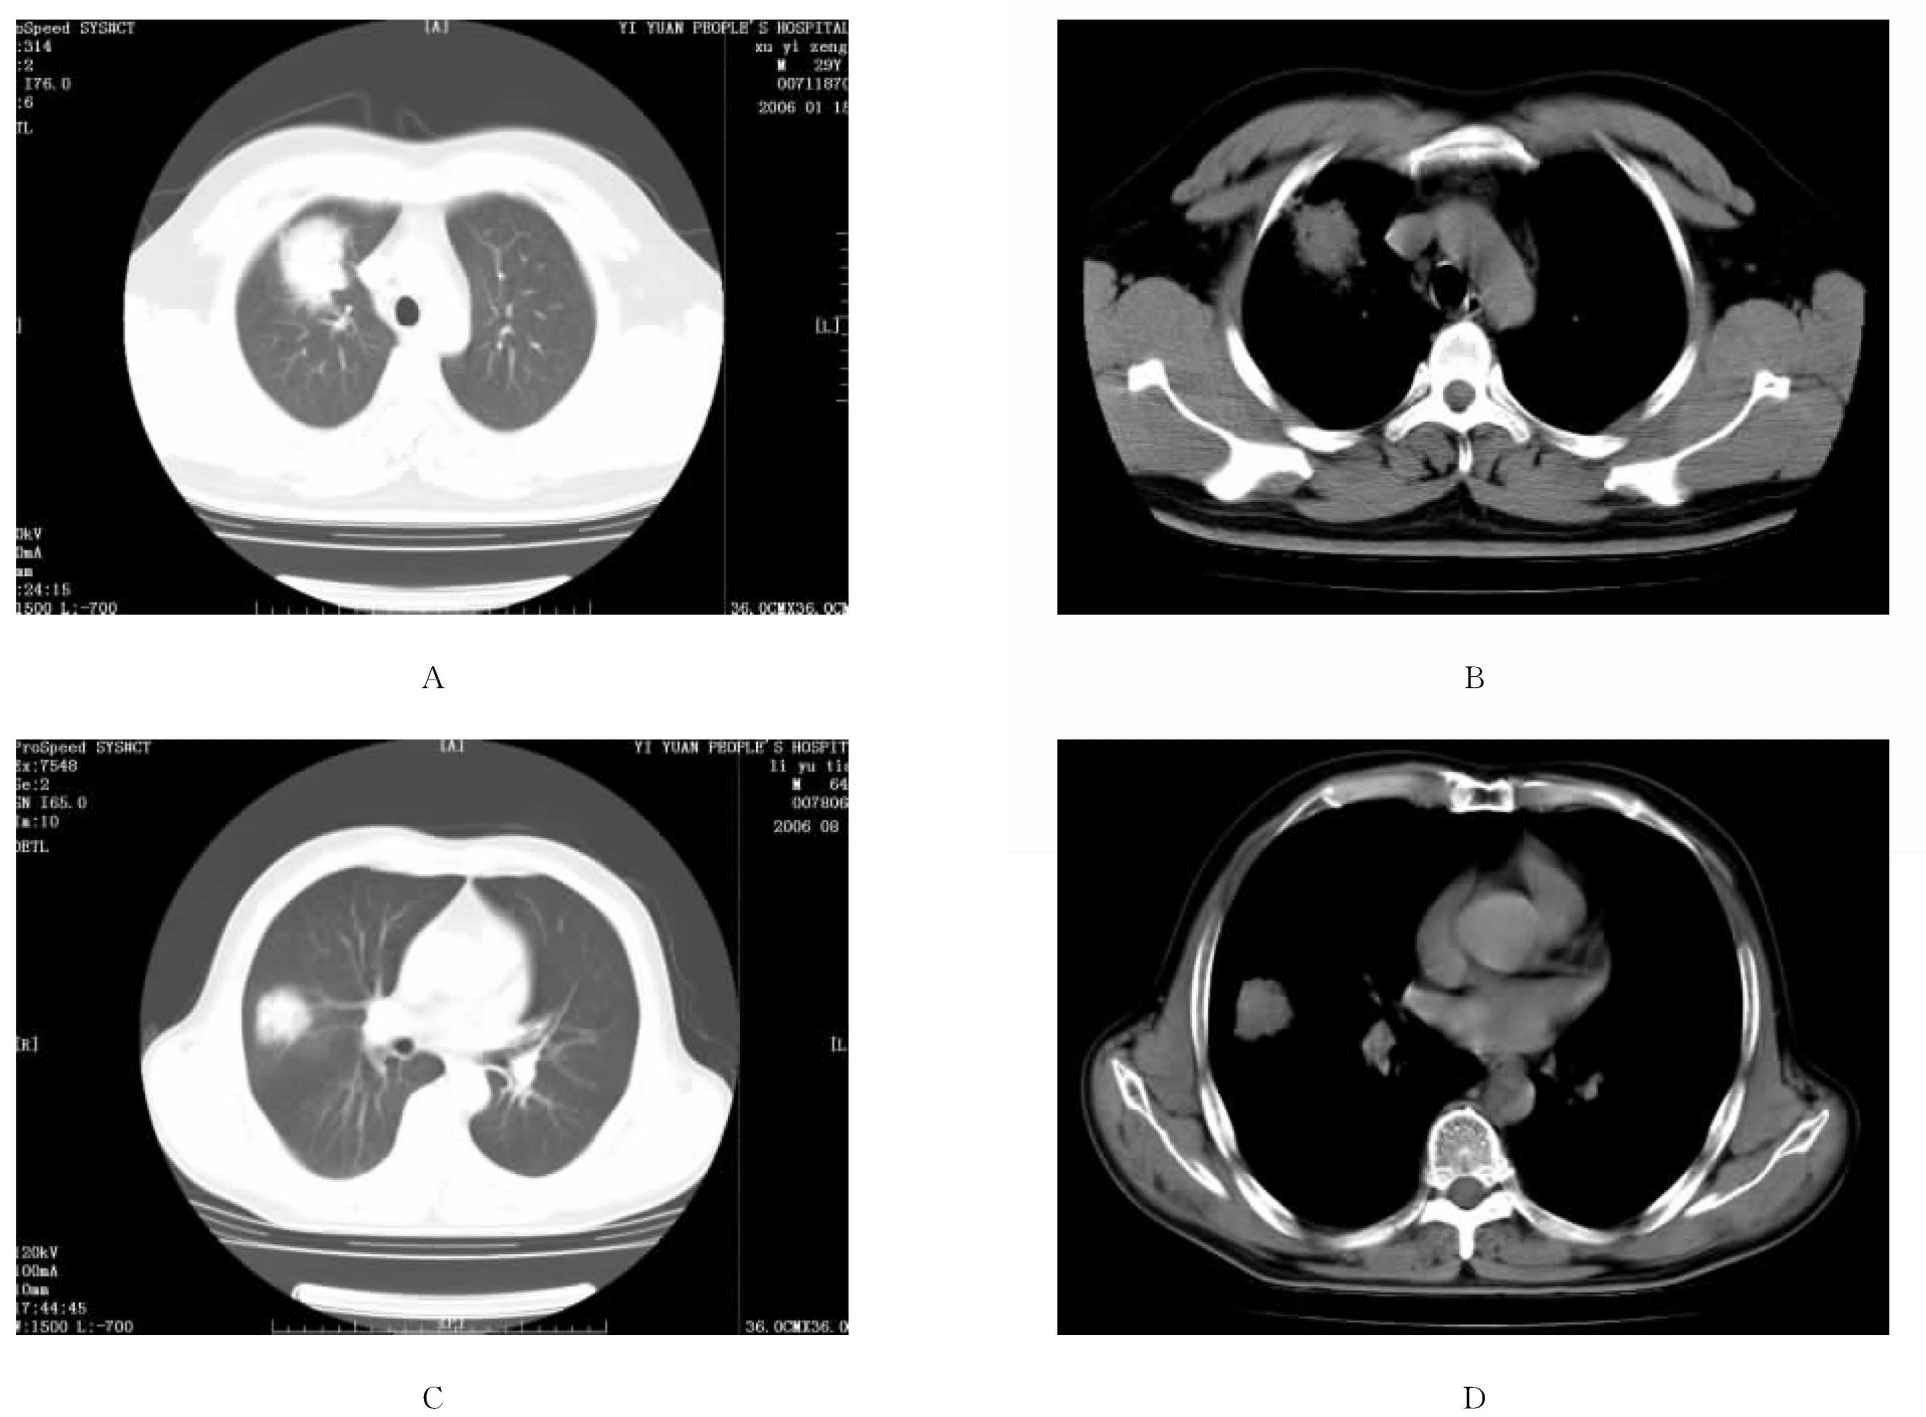
\includegraphics[width=.7\textwidth,height=\textheight,keepaspectratio]{./images/Image00203.jpg}
 \captionsetup{justification=centering}
 \caption{球形肺炎\\{\small A、B为同一患者,病变中央密度较高,周边密度较淡,呈晕圈样改变,无短细僵直毛刺(有粗长柔和的毛刺);纵隔窗显示病灶边缘较平直、无张力,无分叶征。C、D为同一患者,边缘呈晕圈样改变,无短细僵直毛刺;纵隔窗显示病灶边缘平直,无分叶征}}
 \label{fig9-18}
  \end{figure} 

\textbf{【鉴别诊断】}

1.周围型肺癌:①CT多表现轮廓清楚,无晕圈样改变、刀切样边缘(方形征);多有深分叶、锯齿征及短细毛刺。②其边缘多不模糊,多无卫星病灶。少数病例于胸膜侧可有小片状模糊影,为节段性小(细)支气管阻塞性炎症和肺不张表现;亦可于胸膜侧呈片状或楔形模糊绒毛征,为瘤体直接压迫或阻塞肺静脉、淋巴管使其回流受阻所致。在非胸膜侧多无模糊小片状影。③病变周围的胸膜改变多局限,呈胸膜凹陷征或皱缩样改变。④可有血管集束征,集束的血管常有僵直牵拉感(与病变结缔组织增生有关)。此外,结合临床有无急性上呼吸道感染症状可予以鉴别。但某些球形肺炎边缘有分叶、毛刺,甚至临床表现不典型,易误诊为肺癌。

2.结核瘤:病程长、密度高、边缘清楚,其内有点状、片状或分层状钙化,周围有卫星灶。

3.肺良性肿瘤:边缘光整清晰,多无分叶征、毛刺征、锯齿征,邻近胸膜无增厚,周围无充血、水肿、渗出表现,不难鉴别。

\subsection{局限性慢性肺炎}

肺炎病程在4周以上未完全吸收者称慢性肺炎。慢性肺炎常由于病人年龄大、治疗不及时、病原体的耐药性及免疫力功能低下等演变而成;有些无明确急性肺炎病史。

\textbf{【病理】}
慢性肺炎其诊断标准为慢性炎性细胞即单核巨噬细胞浸润及成纤维细胞增生,伴有不同的纤维化及肉芽组织形成,可有肺组织正常结构的破坏。本病从病理上分为:化脓性和非化脓性。慢性肺炎从病变范围上可分为:①局限性:影像学上呈肿块状、肺段或肺叶实变。②弥漫性:呈弥漫性间质性病变,多为慢支反复感染所致。

\textbf{【临床表现】}
以50岁以上男性多见。局限性慢性肺炎以咳嗽、胸痛、痰中带血多见,WBC多在正常范围。根据临床表现,较难与肺癌鉴别。

\textbf{【CT表现】}
局限性慢性肺炎的影像学表现为结节、肿块及肺叶、肺段的实变。

1.肺内结节、肿块样病灶:①部位:国内有报道贴近胸膜(包括叶间裂者)占大多数(65%),并有40%呈长轴贴近胸膜,少数亦可包绕、紧贴胸主动脉。②形态、轮廓:常呈扁平状形态,无膨胀感,且宽基底贴近胸膜,是支持肺炎的重要指标。有时病变中心层面与邻近层面比较,其形态有明显改变。轮廓可光整或呈波浪状、锯齿状,甚至极不规则呈脑沟回状。③边缘及周围结构:边缘可模糊或清楚,可有粗长毛刺。病变周围可有毛玻璃样晕环、增粗血管影通入(通常认为见于肿瘤,但并非肿瘤之特征)、长条索影、局部胸膜肥厚。④密度:可见充气支气管征、空洞、空泡、病变内低密度(主要是化脓性所致)及钙化等。⑤增强扫描(其表现见局限性机化性肺炎)。上述表现与局限性机化性肺炎并无本质区别。

2.肺叶、肺段的实变:体积缩小而根部(肺门侧)无肿块,实变区内有含气的支气管扩张、充气及支气管狭窄扭曲。总之,病史较长的节段性或大叶性实变而根部无肿物者应首先考虑慢性肺炎。

\textbf{【鉴别诊断】}
①结节、肿块样慢性肺炎:缺乏周围型肺癌的典型边缘征象(分叶征、毛刺征等)。而且各边缘征象不同,如有的边缘似分叶,其他边缘无分叶;有的边缘形似毛刺,而其他边缘模糊、并无毛刺。化脓性者强化可较明显,并可见脓腔;也有的增强后鉴别困难。②肺叶、肺段实变阴影的慢性肺炎:多无支气管狭窄和梗阻(支气管轻度狭窄者较难诊断),可有支扩,且无肺根部肿块。但中心型肺癌和肺炎样肺癌亦可无明显支气管狭窄和梗阻,需纤支镜确诊。

\subsection{局限性机化性肺炎}

肺实质及肺间质的纤维化和炎性细胞浸润称为机化性肺炎。

\textbf{【病理】}
机化性肺炎从病理上分为以实质为主的病变和以间质为主的病变。但其基本病理表现是一致的。共同的诊断标准是:①肺实质即呼吸性细支气管、肺泡管及肺泡腔内的炎性渗出物机化,代之以纤维母细胞、肌纤维母细胞增生。②在机化性肺炎部位可见到炎性细胞浸润,主要为淋巴细胞,还有浆细胞和单核细胞。③肺间质的改变为肺泡壁、小叶间隔、支气管血管束周围的纤维组织增生及炎性细胞浸润。这些机化性病理改变不仅见于肺炎,还可见于结核、结缔组织疾病、过敏性肺炎等多种疾病的边缘。

\textbf{【临床表现】}
在临床上机化性肺炎可分为原发性和继发性。原发性中有的为隐源性;继发性是在慢性结缔组织病、血液系统恶性肿瘤、结核病以及应用某些药物的基础上伴发。从机化性肺炎的范围上可分为局限性和弥漫性。其中弥漫性多为隐源性,可表现为阻塞性细支气管炎并机化性肺炎(BOOP)。因而机化性肺炎的临床症状取决于肺内病变是原发性还是继发性,是局限性还是弥漫性。有些可无临床症状,部分病人可有发热、咳嗽及咯血等症状。弥漫性以呼吸困难为主。

\textbf{【CT表现】}

\subsubsection{CT分型和表现}

国外有学者根据病变的部位、形状等将局限性机化性肺炎分为3型:①类圆形:病变为2cm以下的圆形或类圆形结节影,边缘不规则,病变与胸膜及支气管血管束都不接触。②沿支气管血管分布型:表现为卵圆形病变,沿支气管血管束分布。③胸膜带状阴影型:表现为肺野周边的团块状影,病变基底位于胸膜并与胸膜粘连,边缘平直并可出现向心性凹陷。后两型有助于对局限性机化性肺炎的定性诊断。此外,还可有不典型的形状:如三角形、菱形及斜方形等均可提示病变为良性。相关支气管壁增厚、支扩均可提示其炎性性质。

\subsubsection{CT增强扫描表现及与其他疾病的区别}

1.增强值的大小:增强后结核性肉芽肿无明显变化,而炎性病变和恶性病变均明显强化,且炎性病变的峰值多高于恶性肿瘤。通常认为增强峰值<16Hu为良性,16~24Hu为不定性结节,>25Hu高度怀疑为恶性,>60Hu多为炎症。亦有人把20~60Hu作为恶性结节的诊断指标。但中央部坏死或产生黏液的细支气管肺泡癌增强值亦可<16Hu;良性病变(如硬化性血管瘤)亦可增强值>20Hu。还有学者认为炎性结节和恶性结节均可表现为均匀或不均匀强化,两者强化幅度均以20~60Hu多见,其强化幅度无显著差异,即使用下述的强化曲线和峰值出现时间鉴别亦价值有限。

2.时间-密度曲线:炎性结节呈小锯齿状或不规则形且强化持续时间长,与恶性肿瘤的强化曲线呈抛物线状有别,以此判断可能优于增强值。但国外有学者认为炎症呈速升-速降型强化曲线。近期国内有学者用2.5~3.5ml/s流率、注射100ml造影剂发现,肺癌呈缓慢持续升高型,其强化高峰在75s;炎性结节呈逐渐上升型,其强化高峰在135s;结核球呈平坦型,无明显强化高峰。

\textbf{【鉴别诊断】}
与周围型肺癌的鉴别常较困难,与1cm以下周围型肺癌的鉴别尤为困难。①与胸膜接触面广,呈楔形或多角形。病灶一边或多边向心性弓形凹陷。边缘多毛糙,有粗细不均、长短不一的毛刺。支气管壁增厚、支扩以及胸膜增厚和伴随的卫星病变等征象。而无边缘深分叶、短细僵直的毛刺等有助于与肺癌鉴别。②良性病变可与血管无关或血管从病变旁边通过;而恶性病变时常有血管卷入及血管从病变中穿行(但并非恶性所特有)。增强扫描的上述特点可能有助于鉴别。

\subsection{肺炎性假瘤}

肺炎性假瘤的定义含糊,包括很多名称如黄色瘤、黄体瘤、硬化性血管瘤、组织细胞瘤、黄色肉芽肿、浆细胞瘤、假性淋巴瘤。其本质是增生性炎症。

\textbf{【病理】}
其基本组织学改变是以淋巴细胞和浆细胞为主,还有成纤维细胞、异物巨细胞、组织细胞及泡沫细胞等组成的肉芽肿,纤维组织、支气管肺泡上皮及血管增生是增生组织的主要成分,肉眼呈肿瘤样,故称之为炎性假瘤。界限清楚者多有假包膜;而界限不清的无假包膜者,周围有增殖性炎症和轻微的渗出性炎症。本病可恶变。

\textbf{【临床表现】}
在临床上可无症状,也可有咳嗽,但痰中带血少见。结核菌素试验可为阳性,少数呈强阳性,故不能以此否定炎性假瘤的诊断。由于在形成炎性假瘤前无明确的肺炎阶段,因此诊断比较困难,并易误诊为结核或肺癌。急性肺炎也可呈结节状或肿瘤形状,但抗炎治疗2~4周吸收,而炎性假瘤经3个月或更长时间无变化。

\textbf{【CT表现】}
本病的影像学表现无绝对特征性(图\ref{fig9-19})。①单发多见,多位于表浅部位,多呈圆形或椭圆形。大小不一,直径2~5cm或更大。②多有假包膜,边缘多清晰光滑,有时也毛糙,并有切迹或分叶。③病灶邻近胸膜局限性肥厚。由于病灶邻近胸膜有肥厚牵拉,病灶边缘呈桃尖样突起即桃尖征(尖端指向胸膜),有重要诊断价值。④平扫密度均匀,少数有钙化。⑤增强扫描多为中度均匀强化,持续时间较长。亦可显著强化(国外有学者报道CT值升高约35Hu左右)或强化不著。中心密度有时可较低。⑥一般不合并纵隔、肺门淋巴结增大和胸腔积液;少数可见同侧纵隔、肺门淋巴结轻度增大。

\begin{figure}[!htbp]
 \centering
 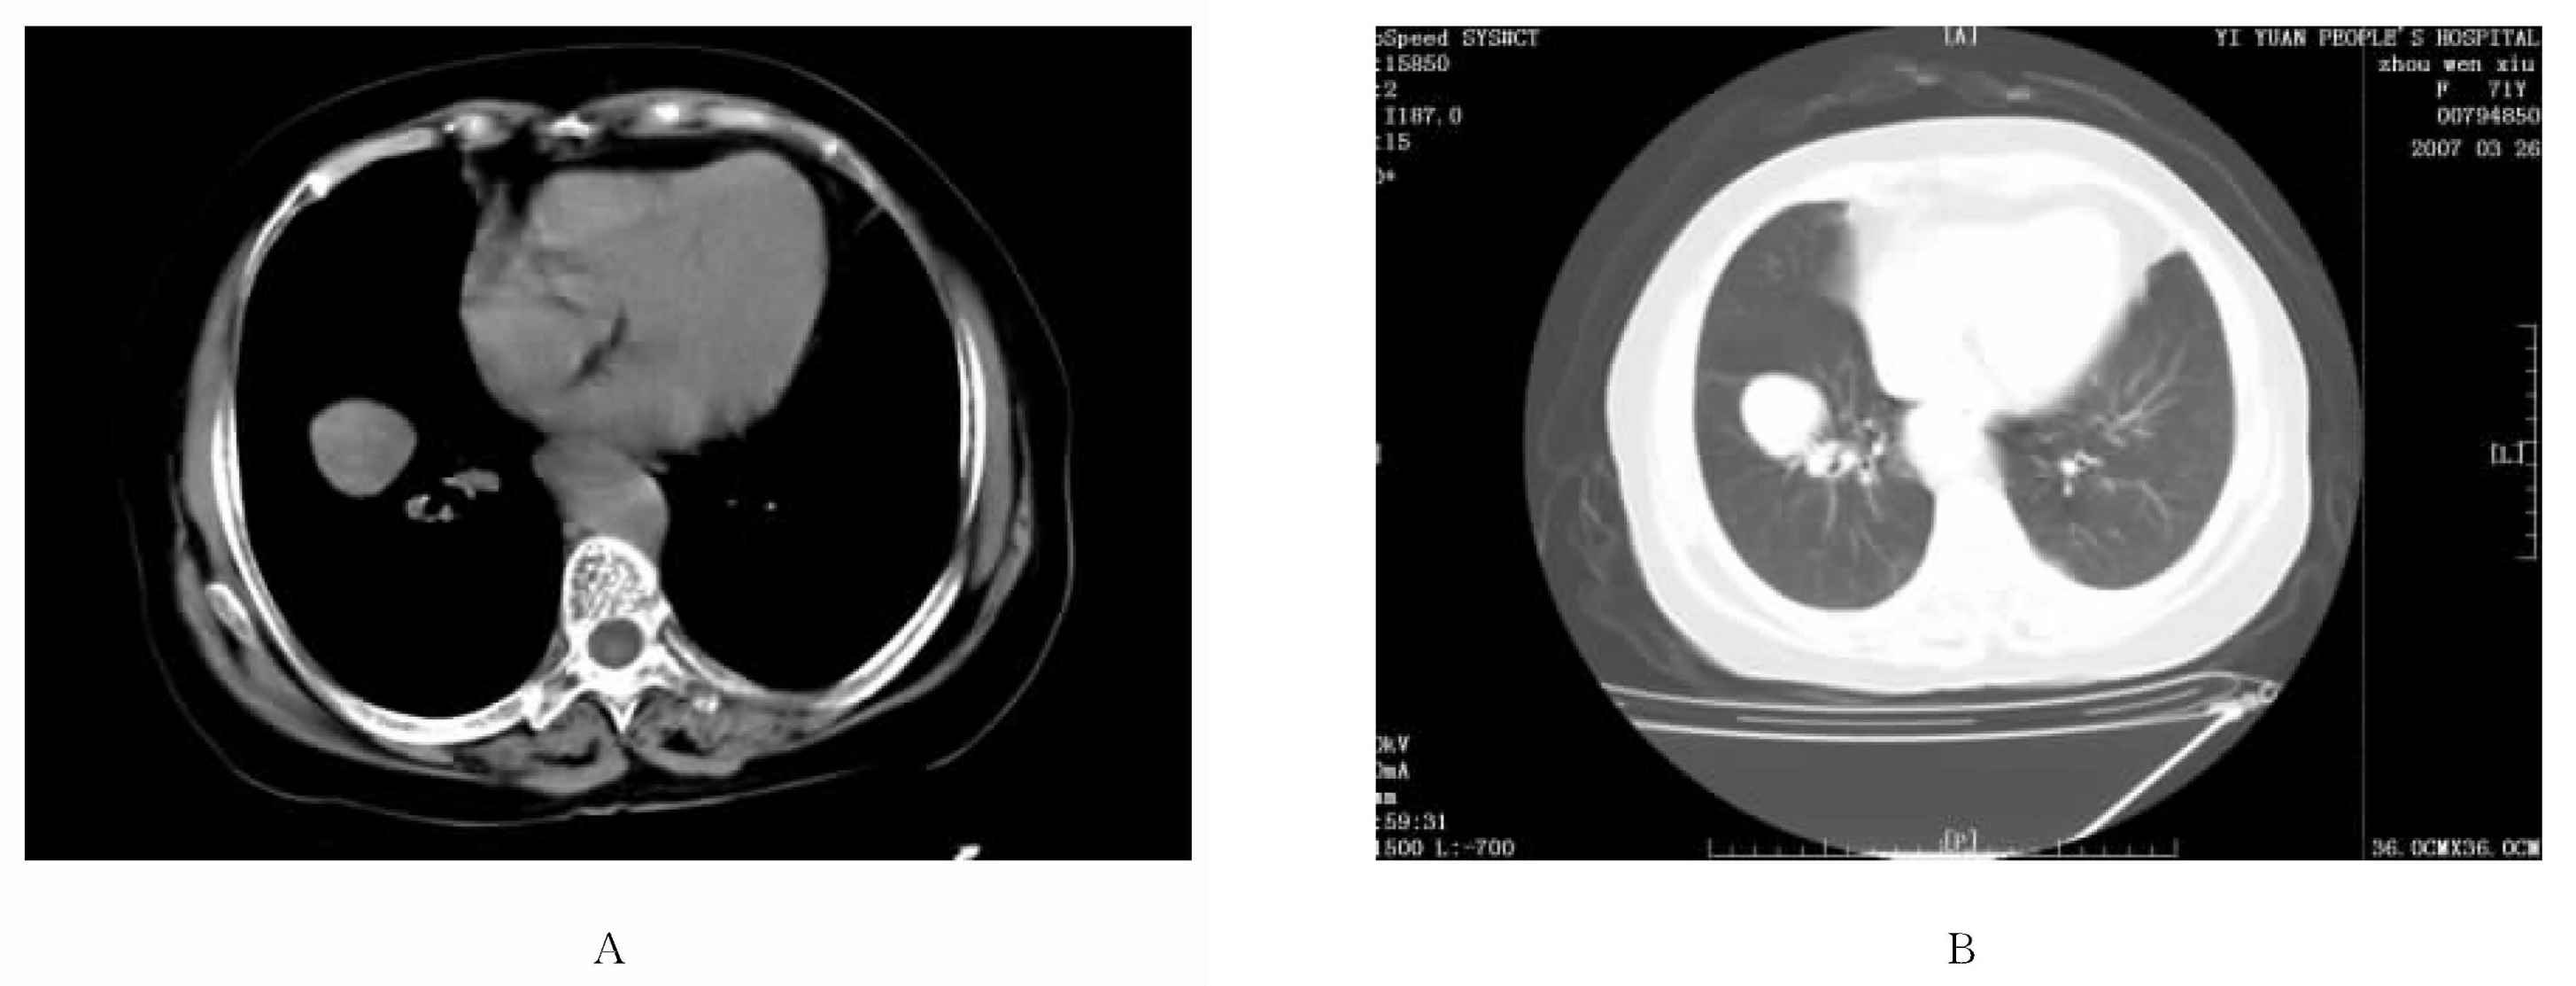
\includegraphics[width=.7\textwidth,height=\textheight,keepaspectratio]{./images/Image00204.jpg}
 \captionsetup{justification=centering}
 \caption{肺炎性假瘤\\{\small A、B为同一患者,右肺下叶前底段近斜裂处有椭圆形高密度灶,边缘光滑,可见桃尖征(指向斜裂)}}
 \label{fig9-19}
  \end{figure} 

\subsection{金黄色葡萄球菌肺炎}

本病的致病菌为溶血性金黄色葡萄球菌。病理及临床分为支气管源性和血源性。

\textbf{【病理】}
①原发性或支气管源性:早期为严重的支气管细支气管炎,其周围有散在的小出血、实变区,可发展为节段性或大叶性,末梢细支气管和肺组织坏死而形成肺脓肿。由于小支气管内有脓液和渗出物存在,常形成小支气管活瓣性阻塞而导致局限性肺气肿,或大的囊样空腔即肺气囊。②继发性或血源性:是其他部位金黄色葡萄球菌感染(如疖、痈、蜂窝组织炎、骨髓炎等)所产生的脓毒败血症,于肺内形成多发性小脓肿。这个过程比较短暂,最终与支气管源性完全一样。

\textbf{【临床表现】}
本病好发于婴幼儿,体弱、多病的成人亦可发病。其临床表现比一般肺炎重,除发热、胸痛、咳嗽、咯脓血痰等外,全身症状较严重,在短期内有全身青紫、末梢循环衰竭征象。部分病人呈慢性迁延性。总之,本病以并发症多、变化快、死亡率高为特点。

\textbf{【影像学表现】}

1.炎性浸润灶:以两肺广泛分布多见。病变大小、形态不一。小者呈粟粒、斑点状,大者呈片状或团絮状。少数呈节段性或大叶性浸润。病变进展迅速,常在较短的时间内出现单发或多发的空洞或液平面。治疗中可见一些病灶吸收,同时又有多数病灶融合或新病灶出现。

2.肺气囊:是本病的特征性影像学表现。在1~2天内即可出现。囊壁薄,其大小、数目和分布可时有不同,甚至一日数变。大者可占据一叶或一侧肺,并对邻近组织和器官产生压迫移位。气囊亦可相互融合。有些肺气囊可见浅小液平面。气囊一般在炎症吸收后消失,也有延至数日后才会消失,消失的过程越长,继发脓肿的机会越多。

当产生多发性含气低密度区时应识别是肺气囊、正常充气的肺,还是空洞。①影像学呈圆形、界限清晰的含气腔隙伴连续光滑薄壁者,应想到是肺气囊;②界限不清的、没有明确的光滑规整边缘的含气区是更典型的重新充气的肺组织;③在实变区中间发生液气平面,且无明确的外壁者,应是组织坏死和脓肿形成。

3.并发症:常见者有胸膜炎、心包积液、支气管胸膜瘘、纵隔气肿、液气胸。肺部炎症早期就有大量胸腔积液、脓胸或脓气胸者,往往提示为金黄色葡萄球菌感染。

\subsection{链球菌肺炎}

本病很少见,常发生于呼吸道感染(包括咽喉部链球菌感染)后。

\textbf{【病理】}
有急性支气管炎、细支气管炎及支气管周围炎,局部有多形核白细胞及淋巴细胞浸润。肺泡及气道内有水肿液、红细胞及病原体,并可见上皮细胞脱落。另一种感染方式是咽喉部链球菌感染经淋巴道向下蔓延到纵隔,发生蜂窝组织炎和淋巴结炎,经肺门向支气管血管束周围、小叶间隔浸润。

\textbf{【临床表现】}
小儿、青年和老年人多见,约1/3在10岁以下。多起病急骤,寒颤、发热、胸痛、咳脓性痰,可闻及湿啰音。

\textbf{【影像学表现】} 它有两种形式:

1.以肺泡实变为主:呈多发斑片状边缘较清楚的高密度影,亦可呈节段性分布的均匀实变。下叶多见,可双侧分布。斑片状病灶有融合倾向,常可出现空洞。少数有气囊,甚或有气胸。

2.以间质改变为主:肺门增大,边缘模糊,表现为细小浸润影自肺门向外扩散,支气管血管束边缘毛糙、模糊,伴细小粟粒状结节。可两肺或局部受累。可有纵隔增宽,伴气管旁或(和)肺门淋巴结增大。有时可见胸腔积液。纵隔的改变是由于咽喉部链球菌感染经淋巴道向下蔓延到纵隔所致。肺的改变由纵隔扩展而来。

\subsection{肺炎克雷白杆菌肺炎}

肺炎克雷白杆菌又称为肺炎杆菌和Friedlander杆菌。

\textbf{【病理】}
其病理过程与肺炎双球菌所致大叶性肺炎相似,但不典型,而且具有化脓倾向。其渗出物比重高而黏稠,内有多核细胞和单核细胞。慢性病例有多发肺脓肿伴肺实质显著纤维化、胸膜增厚。

\textbf{【临床表现】}
多见于中老年人,男性多见。很多病人有肺部慢性疾病、糖尿病或体质衰弱。急性患者多数突然起病,痰黏厚、黄色或呈巧克力色,有时带血丝。

\textbf{【影像学表现】}
主要是炎性实变,有累及多叶及两肺的倾向。病灶多为大叶实变,呈肺段或大叶性分布,呈大叶实变者右上叶多见。病变区密度相对较高,边缘相对清楚,常见叶间裂膨出较为特殊,如有化脓可形成空洞。实变呈小叶分布者,呈散在斑片状影,累及多个肺段或两肺,亦可形成空洞。本病易产生胸膜反应。急性期实变范围广泛者,恢复后常有较多的纤维收缩及广泛的胸膜增厚。

\subsection{军团菌肺炎}

1976年7月,在美国费城举行退伍军人大会期间,与会人员和附近居民中相继出现以发热、寒颤、胸痛、呼吸困难和腹泻为主症的病例。经研究证实,它是由嗜肺军团杆菌所引起,被称为军团杆菌病或军团病。它是一种以肺炎为主的全身性疾病,可散发也可局部流行。

\textbf{【临床表现】}
本病多见于年老体弱或伴严重原有疾病的患者。可有咳嗽、发热寒颤、胸痛、呼吸困难、肌肉关节痛。WBC可升高或降低,血沉增快。可伴有消化(腹痛和腹泻)、泌尿及神经系统症状。

\textbf{【CT表现】}
①肺外周圆形或小斑片状影;②多发斑片影;③叶、段实变;④叶、段不张;⑤局限或弥漫性磨玻璃样高密度影;⑥约10%可形成表现多样的空洞;⑦似间质性肺炎或肺气囊形成似金黄色葡菌球菌肺炎;⑧胸膜肥厚或积液发生率高(32%~63%);⑨少数可伴心包积液和纵隔淋巴结增大。总之,军团菌肺炎CT表现呈多样性,以及多叶、段受累为特点,常合并胸膜病变。

\subsection{革兰氏阴性杆菌类肺炎}

从20世纪60年代至90年代,肺炎致病菌发病率经历了肺炎球菌→金黄色葡萄球菌→革兰氏阴性杆菌类肺炎的演变过程。目前,革兰氏阴性杆菌类肺炎占原发性肺炎的20%,占继发性肺炎(医院内获得)的40%~60%。

\textbf{【病因病理】}
常见的致病菌有大肠杆菌、绿脓杆菌、肺炎杆菌、变形杆菌、流感杆菌、假单胞杆菌等。本病是一种坏死性支气管炎,以支气管肺炎表现形式多见。

\textbf{【临床表现】}
多见于中老年人,男性多见。可有咳嗽、发热、胸痛等,WBC升高。可有原发疾病如慢支、脑血管病、恶性肿瘤、糖尿病等。

\textbf{【影像学特点】}
①病变多为双侧广泛分布的结节状和斑片状高密度灶,易累及双肺下叶,而且部分病例呈多叶、大片状肺实变影;②易早期形成空洞,常为直径<2cm的多发空洞,少有液平面;③可有肺气囊形成;④约40%伴有少量胸腔积液;⑤短期内复查病变范围可扩大或数目增多;⑥病变吸收较慢,并形成纤维化。

\subsection{肺炎支原体肺炎}

本病由肺炎支原体致病,过去所谓非典型肺炎以肺炎支原体多见。

\textbf{【病理】}
基本病理改变为化脓性细支气管炎和肺间质炎症,支气管黏膜充血水肿,单核细胞和淋巴细胞浸润,可有上皮细胞脱落。肺泡壁及小叶间隔有中性粒细胞、单核细胞浸润,肺泡内有炎性渗出物。电子显微镜可发现支原体存在于支气管内及支气管周围的间质浸润病灶中。

\textbf{【临床表现】}
多见于冬春之交或夏末秋初,在学校和部队可有流行性发病。以儿童、青年多见。发病前常有鼻炎、咽炎等前驱症状,一般起病温和,约1/3无明显症状。常有中度发热,少数可高热,一般无寒颤,头痛常见、有时剧烈。顽固性剧咳为突出症状,可伴少量黏痰,有时呈黏液脓性或血性痰。少有胸痛。实验室检查白细胞总数正常或略高,发病后2~3周血冷凝集试验比值升高(可达1∶64)。

\textbf{【CT表现】}
本病影像学表现以肺间质炎症为主,并可呈实变表现。呈现为片状和融合性支气管肺炎或间质性肺炎伴急性支气管炎。CT以斑片状磨玻璃样密度最常见,还可见边缘模糊的肺实变、“树芽征”、小叶间隔增厚、支气管血管束增粗及淋巴结增大。少数有多发病灶或病灶有迁移表现。还有少数如治疗不及时可发生肺脓肿。胸水和淋巴结肿大少见。

\textbf{【鉴别诊断】}
①少数病人临床症状明显,有发热(可持续性高热)、胸痛、咳嗽和白细胞计数升高,此时需与细菌性肺炎鉴别。随访示冷凝集试验结果升高或培养得到病原体有助于鉴别。②支原体肺炎有多发病灶或病灶有迁移表现者需与过敏性肺炎鉴别。但支原体肺炎周围血象中嗜酸粒细胞计数不高,且过敏性肺炎吸收更快、迁移现象显著可资鉴别。必要时需通过冷凝集试验或培养肺炎支原体作鉴别。

\subsection{婴幼儿腺病毒肺炎}

本病是婴幼儿期最常见的病毒性肺炎之一。

\textbf{【病理】}
主要病理改变为坏死性支气管炎和支气管肺炎。支气管壁和肺泡壁坏死,坏死物质堵塞支气管腔。支气管及其周围肺泡有明显水肿、出血及单核细胞和淋巴细胞浸润。于增殖的肺泡上皮内可以见到典型的核内包涵体。腺病毒还可侵袭循环、消化、神经及泌尿系统。

\textbf{【临床表现】}
多见于7个月~2岁的婴幼儿。常为散发,也可发生流行。多起病急骤,中毒症状重,有高热、咳嗽、喘憋、呼吸困难、面色苍白、神萎嗜睡。肺有实变体征和湿啰音。易发生中毒性心肌炎、心衰和中毒性脑病。WBC正常或偏低,以淋巴细胞为主,常有异常淋巴细胞出现。

\textbf{【影像学表现】}
发病1~2天内可见支气管血管束增粗。一般于3~6天出现较大的片状高密度灶,密度较低、均匀,可占据一个肺段或近乎整个肺叶。轻者呈斑片状高密度灶,部分亦可融合成片。同时可见小叶间隔增厚等间质性异常改变。本病吸收缓慢,多在3~6周,重者4~12周开始吸收消散。多遗留间质纤维化改变,少数后遗支扩。

总之,婴幼儿期如表现为肺段或肺叶性实变,应结合临床考虑到腺病毒肺炎。此外,少数腺病毒以及其他病毒感染如呼吸道合胞病毒、巨细胞病毒、麻疹病毒等以间质肺炎为主,CT表现间隔增厚和网状结节改变,累及小叶时呈磨玻璃样密度,应注意认识和诊断。

\subsection{呼吸道合胞病毒肺炎}

本病也是婴幼儿期最常见的病毒性肺炎之一。

\textbf{【病理】}
毛细支气管炎型表现为细支气管上皮增生、水肿和坏死,形成阻塞性毛细支气管炎。间质伴肺泡炎型除上述病理改变外,支气管、血管周围间质和肺泡腔内有水肿、细胞渗出和坏死。

\textbf{【临床表现】}
上呼吸道感染后2~3天出现肺炎症状。约70%为轻症病例,重症病例中2/3为6个月内幼婴,1/3为新生儿。主要表现为发热、咳嗽和呼吸困难,肺部可闻及湿啰音及喘鸣音。

\textbf{【影像学表现】}
①毛细支气管炎型以阻塞性肺气肿为主要征象,病变广泛累及两肺,有时可见广泛间质结节。②间质肺炎型可有支气管血管束增粗、毛糙,以及小叶间隔增厚等间质性异常改变,伴有小斑片状、磨玻璃状高密度灶,广泛累及两肺内中带,同时两肺有显著肺气肿。

本病吸收消散约1~2周,病变吸收后不留任何痕迹。

\subsection{严重急性呼吸综合征(SARS)}

本病是于2003年全球流行的一种新的危害性极大的呼吸道疾病,我国命名为传染性非典型性肺炎,WHO将其命名为严重急性呼吸综合征(severe
acute respiratory syndrome,SARS
)。它是由新型变异的冠状病毒(SARS-CoV)感染引起的一种具有明显传染性、可累及多个脏器系统的特殊肺炎。SARS在我国首发病例于2002年11月的广东省,随后在当地引起一定规模的局部流行,然后疫情蔓延至25个省份。WHO于2003年4月16日正式宣布引起SARS的病源为冠状病毒属中出现的一种新病毒,并正式命名SARS
Virus。

\textbf{【临床表现】}
起病急,多以高热为首发症状。偶有畏寒,可有全身酸痛、乏力、腹泻,还可有咳嗽,多为干咳,偶有血丝痰。胸部影像学检查可见肺部炎性浸润;实验室检查外周血WBC计数正常或降低;抗生素治疗无效是其重要特征。重症病例表现明显的呼吸困难,并可迅速发展成为急性呼吸窘迫综合征。

\textbf{【诊断标准】}
主要依据2003年5月中华人民共和国卫生部和WHO颁布的诊断标准:①发病前两周有密切接触史或生活在流行区;②有发热(>38℃)、咳嗽、气促、呼吸窘迫、肺部啰音;③早期WBC计数正常或降低;④X线示肺部出现斑片状浸润灶;⑤抗生素治疗无明显效果。

总之,结合流行病学史、临床症状和体征、一般实验室检查、胸部影像学变化,配合SARS病原学检测阳性,排除其他类似疾病,可以作出SARS的诊断。具有临床症状和出现肺部影像学改变是诊断SARS的基本条件。流行病学方面有明显支持证据和能排除其他疾病,是能够作出临床诊断的最重要支持依据。

\textbf{【影像学表现】}

1.X线表现:①早期:于发病1~11天(平均3天),出现肺实质和肺间质异常。前者表现为双下肺中外带斑片状阴影,密度较淡、边界模糊,部分呈磨玻璃样。此期主要病理变化是肺泡和细支气管周围渗出性改变。②进展期:于发病后6~23天(平均8天)。表现为病灶增多、相互融合、范围扩大、密度增高,呈界限不清的大片实变影。此期病理表现为大量炎性细胞浸润,大量纤维素和蛋白渗出,肺泡间隔增宽。如得不到及时、有效治疗,会迅速发展为进行性纤维化或机化,导致呼吸窘迫而死亡。少数病例其病灶有游走现象。无钙化、空洞、胸腔积液、淋巴结增大。③消散期:肺部阴影逐渐完全吸收或仅遗留下少许纤维条索影。首次发现胸部异常到病变消散持续时间为7~46天,平均19天。

国内有学者将其X线表现分为5型:①单纯局限型:由单一局部病灶(片状、类圆形肺实变)到范围扩大(涉及范围≤2个肺野)或无明显继续增大;②局限-广泛型:单一局部病灶迅速发展为广泛分布(≥3个肺野);③多发型:早期即为多发(≥2个)结节状、片状或(和)团片状病灶,其后病变扩大或发展至广泛分布,形成双侧或单侧多发实变;④间质-实质型:早期以间质性炎症为主,并可有少许肺实质浸润,其后迅速出现明显的肺实质病变;⑤间质型:以肺间质渗出改变为主要表现。

2.CT表现:与平片所见一致,呈单发或多发片状磨玻璃样阴影、明显实变影,边界模糊,倾向于下叶及外周分布,可伴叶间裂、小叶间隔增厚。肺部弥漫性点状阴影,浸润阴影可以掩盖血管纹理(亦可不)。少数表现为伴有空气支气管征的、界限清楚的实变阴影,整叶的实变影少见。对心后脊柱旁区病变的观察优于平片。

\subsection{流行性出血热}

\textbf{【病理】}
其病变为毛细血管扩张充血、通透性增加和血浆渗出。肺实质有出血和水肿。

\textbf{【临床表现】}
主要为高热、皮肤黏膜出血点、蛋白尿、血小板减少。患者呈醉酒貌。临床分为发热、低血压、少尿、多尿和恢复5期。

\textbf{【影像学表现】}
①肺充血:为早期表现,肺门影增大,支气管血管束模糊;②肺水肿:可呈泡性和间质性水肿;③胸膜改变:一侧或双侧少量或中量胸腔积液,以及胸膜增厚粘连;④心影增大;⑤病灶变化快,一般于2~8天内吸收消散。

\subsection{恙虫病}

立克次体病涉及呼吸系统者主要为恙虫病及Q热。恙虫病鼠类是其主要的传染源,恙螨幼虫是其传播媒介。病原体在恙螨体内繁殖经卵传至第二代,次幼虫亦可通过叮咬人或动物而传播。Q热野鼠和家畜为其主要传染源,蜱为传播媒介。

\textbf{【病理】}
立克次体病的主要病理改变是受累器官的急性间质性炎症、血管炎及血管周围炎。实质器官充血、水肿,细胞变性,以致灶性坏死。有人认为立克次体被吞噬细胞溶解后,其降解产物作为一种变应原,引起机体超敏反应而致多个器官受损害。

\textbf{【临床表现】}
国内有资料统计恙虫病发病年龄在1.5~80岁,平均30岁,6~9月份为发病高峰,以农民野外作业为多见,次为学生。表现为高热(100%),热程3~14天。皮肤焦痂和溃疡(70%)、皮疹(40%)、淋巴结增大(50%)、全身酸痛(72%)、腹痛腹泻(12%)、尿频尿急(15%),少数可有脑部症状。实验室检查:少数WBC可升高、血小板减少、ESR常增快,尿检常有蛋白、管型、白细胞及红细胞,肝、肾功能可有损害。血清外-菲氏反应多为阳性。

\textbf{【CT表现】}
恙虫病有肺部异常影像学表现者近40%,①肺间质和肺实质炎症:肺渗出性病变可呈小斑点状、斑片状、磨玻璃状、大片状;②少数可有空洞形成及胸腔积液;③可见肺门淋巴结增大;④可涉及心肌和心包,出现心脏增大及心包积液;⑤此外,还可有肝、脾增大,甚至脑出血。

Q热与上述表现相似,但无淋巴结增大。还应注意密切结合临床与钩端螺旋体病鉴别。

\subsection{肺钩端螺旋体病}

本病以四川和广东流行较广。多见于农民和青壮年。接触疫源者均可发病。

\textbf{【病因病理】}
鼠类和猪是钩端螺旋体的主要宿主,由于食入带病原体的动物,或由这些动物污染的水和食物而致病。钩端螺旋体的毒素能使广泛的末梢血管产生严重的变性松解,造成不同程度的出血。显微镜下虽可见到一些白细胞浸润及吞噬细胞活动,但无明显的炎症性病变的表现。最为突出的是局部或广泛的肺内出血和水肿。

\textbf{【临床表现】}
本病潜伏期短,起病急骤。病人畏寒高热,继之全身肌肉酸痛,以腓肠肌疼痛最为明显。肺部症状为咳嗽、咳血,甚至呼吸急促、胸闷等。

\textbf{【影像学表现】}
本病的影像学表现无特异性。发病后24~72小时后出现表现,5~10天内大部分吸收。早期表现为支气管血管束模糊,进而有磨玻璃样渗出。进一步发展可见比较小的斑片状局部渗出灶像支气管肺炎,也可呈大片或节段分布。还可见两肺弥漫的斑片状、结节状影,直径2~5mm,以中下部为多。病灶分布可稀、可密,以外带较密集。

\subsection{吸入性肺炎}

按照吸入方式和吸入物质的不同可将吸入性肺炎分为:①急性吸入性肺炎;②慢性吸入性肺炎;③类脂质肺炎;④羊水吸入性肺炎;⑤胎粪吸入性肺炎;⑥呕吐物吸入性肺炎。

\textbf{【病理】}
由于吸入物质的阻塞,可导致阻塞性肺气肿和肺不张。由于吸入物质的化学性和机械性刺激,在支气管和肺内产生无菌性炎症。如吸入物内含有细菌,可产生肺化脓性炎症。

\textbf{【临床表现】}
咳嗽、咳痰、呼吸困难、发热等。其预后因吸入物质的多少、肺炎的严重程度及有无继发细菌感染而异。

\textbf{【影像学表现】}
①急性肺水肿;②阻塞性肺气肿和肺不张;③支气管肺炎;④纤维化、肉芽肿及“石蜡瘤”,后者为类脂质肺炎(即吸入矿物类如液体石蜡等)慢性阶段的表现;⑤肺脓肿。其中肺不张、纤维化及肺脓肿为慢性吸入性肺炎的3个常见并发症。慢性吸入者可发展为蜂窝样影。

总之,吸入性肺炎无特征性影像学表现,需密切结合病史始能作出病因诊断。

\subsection{内源性脂性肺炎}

本病亦称为胆固醇肺炎,系胆固醇沉积所致的肺泡炎症及间质纤维化改变,是一种少见疾病,远较因吸入油类所致的外源性脂性肺炎少见。

\textbf{【病因病理】}
其病因尚不清楚,可以原发,也可继发于肺部慢性疾病。有人认为可能由于慢性肺疾病如肺炎、结核、癌肿等病因刺激使肺泡上皮细胞大量破坏,胆固醇等类脂质变性释放,并被组织细胞吞噬形成泡沫细胞沉积在肺泡腔内或肺泡壁所致;也有人认为是吸烟引起Ⅱ型肺泡上皮细胞内形成或含胆固醇过多所致。病变多累及肺段或叶,其体积常有缩小,胸膜常增厚并钙化,病变进展时呈现纤维化、小支气管扩张及慢性支气管炎样改变,但极少有肺泡钙化。总之,本病在组织学上早期主要为肺泡腔和肺泡管内充盈大量泡沫细胞(大单核细胞),晚期可累及肺泡间隔导致其纤维化及细支气管炎改变。

\textbf{【临床表现】}
多见于40~60岁,男女之比为4∶1。以发热、咳嗽、胸痛、血痰为主要表现。

\textbf{【CT表现】}
①肺段或肺叶实变型:按肺段或叶分布的实变、浸润并呈扇形或三角形,近肺门侧密实,外界淡薄,其内可有含气支气管,实变区CT值低(≤10Hu)。②肿块型:肿块呈分叶状,伴粗毛刺;无明显胸膜牵拉征象,局部胸膜增厚;肿块CT值较低(≤20Hu)。③肺不张型:按肺叶或段分布,合并病灶周围小结节影及条索影。此外,有报道本病可合并纵隔淋巴结增大。

本病最终确诊依赖于肺活检或术中病理发现泡沫细胞。

\subsection{间质性肺炎}

\textbf{【病因】}
间质性肺炎按病因分为病毒性肺炎、特发性间质性肺炎、结缔组织疾病性等;按病程分为急性和慢性两种。急性者大多为病毒感染所致,也可继发于化脓性肺部炎症,如百日咳、麻疹和流行性感冒、呼吸道合胞病毒肺炎等。慢性者多继发于肺和支气管的慢性疾病,如慢性支气管炎、支气管扩张、尘肺、结缔组织疾病等。

\textbf{【病理】}
其特征是炎症累及肺间质,沿间质的淋巴管蔓延,可引起局限性淋巴管炎和淋巴结炎。由于小支气管的炎性阻塞,常伴有不同程度的阻塞性不张或肺气肿。慢性间质性肺炎则以间质组织纤维化或肉芽组织形成为主。

\textbf{【临床表现】}
病毒性感染所致者主要表现为发热、咳嗽及气急等症状,而呼吸系体征较少。而特发性多表现为亚急性、慢性的咳嗽和呼吸困难,但其中的急性间质性肺炎(AIP)起病急,有发热、咳嗽和暴发性气短,病人可先出现上呼吸道病毒性感染,几天后可发生严重的用力性呼吸困难,甚至进展为对吸氧无反应的呼吸衰竭。结缔组织疾病性等慢性疾病所致者,有相应的临床症状和体征。

\textbf{【CT表现】}
早期主要表现为弥漫性磨玻璃样密度灶、小叶内间质增厚、小叶间隔增厚、支气管血管束增厚毛糙等,侵犯小气道还可引起气体潴留及亚段性肺不张。晚期或慢性发病者可有胸膜下弧线影、肺内长线影、蜂窝影或牵拉性支扩等。肺门和气管旁淋巴结可增大,少数病例可有少量胸腔积液。

\subsection{特发性间质性肺炎}

特发性间质性肺炎是一种弥漫性的、复杂的非肿瘤、非感染性病变,是由炎症或纤维化引起的肺实质损伤,不仅累及肺间质,也损伤肺实质、外周气道、血管和血管周围结构。因为这类疾病并不只限于间质,病因也不完全是特发性的,故特发性间质性肺炎这一术语并不精确。

\subsubsection{过去的分类}

1969年国外学者把特发性间质性肺炎分为5个类别:①一般性(普通型)间质性肺炎(UIP);②脱屑性(剥脱性)间质性肺炎(DIP);③淋巴细胞性间质性肺炎(LIP);④巨细胞间质性肺炎(GIP);⑤闭塞性细支气管炎伴间质性肺炎(BIP)。上述5型并不代表某一特殊疾病,而是肺组织对各种不同致病因子的不同组织反应,即每一类型可见于多种不同疾病,而某一疾病可以有以上不同的间质性肺炎存在,如类风湿性肺病活检可有UIP或DIP。

UIP是最常见的一种间质性肺炎,其病理特点是间质纤维化和单核细胞浸润。DIP较UIP少见,其病理特点是肺泡上皮损伤为主。UIP以网状蜂房影及小结节影为主。DIP则以斑片、磨玻璃影为主,以中下肺外周为著。LIP多呈磨玻璃影;虽然肺囊腔(壁厚小于1mm)和小结节(小于3mm)少见,但较有特征。

过去认为所谓特发性肺纤维化不属于特发性间质性肺炎,其病因不明。病理上即有典型UIP也有DIP改变。但新的分类将其归为特发性间质性肺炎。

\subsubsection{新的分类}

2002年美国胸科学会和欧洲呼吸学会制定了新的分类。按它们的发生率多少依次是:

1.特发性肺纤维化(IPF)

英国学者曾称为隐源性纤维化性肺泡炎(CFA)。与UIP有相关的组织学和影像学表现。(详见本章第十九节)。

2.非特异性间质性肺炎(NSIP)

NSIP是在将来进一步澄清其本质之前提出的临时性术语。该术语用于识别IIP中的一种有明确特发性、预后较IPF好的类型。

\textbf{【病理】}
组织学可分为3组:①主要为间质性炎症;②有间质性炎症和纤维化;③主要为纤维化。与IPF的区别为病变呈暂时的单一性,表现为一致的、均匀的慢性间质性炎症,Ⅱ型肺泡上皮增生,轻度纤维化和没有蜂窝肺。

\textbf{【临床表现】}
发病年龄比IPF小(后者多>50岁),但可发病于任何年龄组。该病与IPF相比,慢性者较少。病程约几个月到几年,预后较IPF好。病人有咳嗽、呼吸困难,与吸烟无关。一些病例可能与结缔组织病、过敏反应、药源性肺炎和某些感染(如HIV)有关。

\textbf{【CT表现】}
多呈磨玻璃影,其中1/3病例是惟一的征象,常双侧对称性分布,以胸膜下为主;半数可见不规则线状或网状影,可伴牵引性支气管扩张。蜂窝和实变较少见。

3.隐源性机化性肺炎(COP)

即闭塞性细支气管炎伴机化性肺炎(BOOP)。90%病例在CT上可见气腔实变,50%以上呈胸膜下或支气管周围分布(详见本章第四节)。

4.急性间质性肺炎(AIP)

本病也称为弥漫性肺泡损伤。其病理组织学与败血症和休克引起的急性呼吸窘迫综合征(ARDS)的表现相似。AIP必须与结缔组织病、感染(如卡氏肺囊虫肺炎)、过敏反应、尿毒症等的ARDS相区别。

\textbf{【病理】}
组织学有3个不同阶段。第1期为渗出期,表现为肺泡内透明膜形成和间质内散在混杂的细胞浸润。第2期为增殖期,有Ⅱ型肺泡上皮增生。第3期为终末期,是纤维化期,表现为肺泡内疏松的机化性纤维化。

\textbf{【临床表现】}
是一种急性的、持续几天到几周的暴发性肺损伤。病人既往体健,起病急,有发热、咳嗽和暴发性气短,多病情进展迅速,死亡率50%。病人可先出现上呼吸道病毒性感染,如肌痛、发热、寒颤和不适等,几天后可发生严重的用力性呼吸困难,甚至进展为对吸氧无反应的呼吸衰竭。肺功能试验为限制性。

\textbf{【CT表现】}
早期为磨玻璃样密度和肺实变,很快发展为间质纤维化。早期磨玻璃影常呈两侧的斑片状分布,无明确的胸膜下或中心性分布。实变不如磨玻璃影常见,常分布在肺底,偶可弥漫,极少以上叶为主。少数可见小叶内线影和胸膜下蜂窝。随后的机化期可见支气管血管束扭曲和支扩。囊状影和其他的低密度区更常见于晚期。

5.呼吸性细支气管炎-间质性肺病(RB-ILD)

见于吸烟者和前吸烟者。

CT包括小叶中心结节、斑片状磨玻璃影,以及中央和周围气道管壁增厚。上叶小叶中心型肺气肿常见,但不严重。斑片状低密度区是气体潴留所致(详见本章第四节)。

6.脱屑性间质性肺炎(DIP)

DIP累及目前仍吸烟者,并与RB-ILD有许多相似之处,有些人把它看作是RB-ILD的晚期表现。

\textbf{【病理】}
包括肺泡远端气腔内有均匀的弥漫性巨噬细胞积聚,巨噬细胞内含有尘样-棕色色素,与RB-ILD相似。但RB-ILD呈小叶中心分布,而DIP呈弥漫分布。肺泡壁很少增厚,几乎无纤维化。

\textbf{【临床表现】}
好发于目前仍吸烟者。多见于50岁左右,男性是女性的2倍。该病表现呈亚急性,伴咳嗽和呼吸困难,50%有杵状指。肺功能试验为限制性。

\textbf{【CT表现】}
所有病例均有磨玻璃影。73%分布于下肺野,59%分布于外周,23%呈斑片状,18%分布弥漫而均匀。59%肺底部有不规则线影和网影。少于1/3的病例可见蜂窝。

7.淋巴细胞性间质性肺炎(LIP)

\textbf{【病理】}
可见淋巴细胞、浆细胞所致的致密性间质性浸润,肺泡内充满淋巴细胞和Ⅱ型肺泡细胞。沿淋巴管有过度增生的淋巴样细胞聚集,也可以血管为中心。

\textbf{【临床表现】}
发病于50多岁,女性更多见。75%伴有蛋白异常血症。本病发病隐匿,表现为咳嗽和呼吸困难,病程大于3年或更长。可伴发热、体重减轻、关节痛、轻度贫血等。与许多自体免疫性疾病有关。

\textbf{【CT表现】}
常为磨玻璃影,也可见奇异的血管周围囊肿(1~3cm)或血管周围蜂窝。约50%见网影,可发生肺小结节和广泛的实变。

\subsection{小结}

\subsubsection{肺部孤立性炎性病变的CT特点}

有以下CT特点:①两肺下叶背段及基底段较多见,其次为上叶后段,中叶及上叶舌段较少见。②病变形状呈楔形、扁平状。边缘平直、无膨胀表现,甚至呈弓形向心性收缩。但亦可不规则甚至极不规则,且中心层面与相邻上下层面其形态可有显著变化,如中心呈球形,上下层面呈楔形、多角形等。③病变边缘可有粗长毛刺(长>0.5cm)或光滑锐利。病灶边缘多部分清楚、部分模糊,或完全模糊的晕圈征。④肺窗清楚、纵隔窗消失。由肺窗变为纵隔窗面积缩小不到50%,称为不完全消失型。由肺窗变为纵隔窗面积缩小超过50%,称为完全消失型。完全消失型应高度怀疑为炎性结节,但<15mm的腺癌亦可呈此表现。⑤相邻胸膜广泛肥厚粘连,无胸壁浸润表现,胸膜外脂肪清晰。⑥病变邻近可有支扩,周边可有卫星灶。⑦增强扫描强化曲线多呈小的锯齿状或不规则形,且强化持续时间长(但众家学说不一)。

炎性病变无周围型肺癌的典型边缘深分叶征、短细僵直毛刺征、棘状突起和病灶内的空泡征、结节征以及胸膜凹陷征、血管集聚征、血管通入征等表现。但有时炎块亦可有分叶、短毛刺、弓形向心性凹陷之边缘相交处有尖角状突起、胸膜凹陷征、血管集聚增粗甚至通入其中,而难以鉴别。此外支气管充气征、空洞、空泡、病灶内低密度区和钙化等,肺炎和肺癌均可见及。

\subsubsection{局限性慢性肺炎、局限性机化性肺炎、结核性肉芽肿与恶性肿瘤CT增强扫描的区别}

1.平扫:结核肉芽肿的密度最高,炎性病变低于恶性肿瘤。

2.增强值的大小:结核性肉芽肿无明显变化,而炎性病变和恶性病变均明显强化,且炎性病变的峰值多高于恶性肿瘤。通常认为增强值<16Hu为良性,16~24Hu为不定性结节,>25Hu高度怀疑为恶性,>60Hu多为炎症。亦有人把20~60Hu作为恶性结节的诊断指标。但中央部坏死或产生黏液的细支气管肺泡癌增强值亦可<16Hu;良性病变(如硬化性血管瘤)亦可增强值>20Hu。还有学者认为炎性结节和恶性结节均可表现为均匀或不均匀强化,两者强化幅度均以20~60Hu多见,其强化幅度无显著差异,即使用下述的强化曲线和峰值出现时间鉴别亦价值有限。

3.时间-密度曲线:炎性结节呈小锯齿状或不规则形且强化持续时间长,与恶性肿瘤的强化曲线呈抛物线状有别,以此判断可能优于增强值。但国外有学者认为炎症呈速升-速降型强化曲线。近期国内有学者发现肺癌呈缓慢持续升高型,其强化高峰在75s;炎性结节呈逐渐上升型,其强化高峰在135s;结核球呈平坦型,无明显强化高峰。

\subsubsection{晕轮征}

本病也称为晕征。是指密度较结节或肿物中央明显减低的、完全围绕在其周围的环状影。其形成机制主要为炎性渗出、出血、肿瘤细胞浸润。主要见于下列疾病:

1.炎症性疾病:包括肺嗜酸性细胞增多症、特发性嗜酸性细胞增多症、寄生虫感染的嗜酸性肺病、局限性机化性肺炎(不吸收或延迟吸收的肺炎)、球形肺炎。

2.出血性肺结节:①感染性疾病中的出血性结节:包括侵袭性肺曲菌病、毛霉菌病和念珠菌病等许多疾病,还有报道1例结核球并咯血患者CT上有“晕征”。②非感染性疾病中的出血结节:如Wegener肉芽肿,原发和转移性出血性肿瘤如血管肉瘤、Kaposi肉瘤、绒癌和黑色素瘤等。此外,肺子宫内膜异位症亦可见出血性肺结节。

3.肿瘤细胞浸润:如细支气管肺泡癌、其他原发性肺癌、淋巴瘤和某些转移瘤。

但通常认为晕轮征主要见于侵袭性曲菌病。

\subsubsection{节段性和大叶性阴影}

1.肺叶的实变呈均一的或融合的高密度影。纯粹的实变不引起容积的缩小,而且常导致肺叶膨胀。大叶性肺膨胀见于肺炎双球菌肺炎、克雷白杆菌肺炎、假单胞菌属肺炎、葡萄球菌肺炎、结核、癌肿伴阻塞性肺炎。

2.大叶性实变的最常见病因是肺炎双球菌肺炎,另外还有克雷白杆菌肺炎、原发结核、吸入性肺炎、肺栓塞伴水肿、出血或梗死,以及阻塞性肺炎。

3.支气管肺炎的典型表现为多灶性阴影,因有广泛性的支气管侵犯,从而形成节段性或大叶性阴影,但多密度不均,周围肺段或叶仍有多灶影。病毒性和支原体肺炎所产生的节段或大叶阴影的机制可能与此相同。

4.肺炎的细菌学诊断并不是放射医师的主要任务,但仍应注意各类肺炎的共性和特异性表现。如大叶阴影合并弥漫网状结节性间质性病变,应考虑为非细菌性肺炎;肺叶实变膨隆和空洞形成强烈提示为克雷白杆菌肺炎。具有化脓和形成肺气囊倾向的支气管肺炎有金葡菌肺炎、革兰氏阴性杆菌类肺炎及少数厌氧菌肺炎。

5.对已知有好发因素的患者如嗜酒、新近麻醉史、头颈部肿瘤、抽搐、食管运动障碍等,特别要想到吸入性肺炎。

6.原发性肺结核是节段性和大叶性阴影的重要原因,常伴肺门淋巴结增大。这种联合出现在儿童也可见于病毒性肺炎,在老年是诊断肿瘤所致的阻塞性肺炎的一个重要线索。

7.阻塞性肺炎及肺不张是节段性和大叶性实变的一个重要原因。

\subsubsection{一侧肺炎和肺水肿的鉴别}

一侧肺水肿可见于气胸后肺部迅速膨胀引起的复张性肺水肿、充血性心衰、胸部创伤、胃酸吸入、某些先心、DDV中毒。肺水肿的特点是:①局部血管增粗,边缘模糊;②以肺门为中心,沿血管走行分布的斑片状高密度;③病变消失快。

但肺炎其血管无明显改变,病变从一叶发生,也可同时累及几个肺叶。病变由小到大、由少到多,逐渐发展。病变吸收亦是由多到少、有大到小的过程。

\subsubsection{弥漫性融合阴影}

1.弥漫性融合阴影伴支气管气像(即充气征)、肺泡气像(实变肺组织内所包围的含气肺泡和玫瑰花腺泡)构成了肺泡疾病的典型影像学表现。纯粹的肺泡疾病罕见,肺泡蛋白质沉着症是极少见的病例之一。其他多为肺泡和间质性疾病的混合改变,但病变原有的间质成分多被掩盖。

2.弥漫性融合阴影的最常见病因是肺水肿。

3.成人呼吸窘迫综合征可产生弥漫性融合阴影。当患者有严重创伤或休克,特别是药物反应、革兰氏阴性脓毒血症、输液反应、蛇咬伤或心肺转流使用氧气泵等之后出现急性肺水肿,应怀疑这一诊断。

4.弥漫性肺炎是弥漫性融合阴影另一十分重要的疾病。致病菌常为革兰氏阴性菌。病毒、真菌和原虫亦可有此表现。

5.弥漫性肺出血可呈广泛的双侧融合阴影。患者并不一定咳血。诊断需结合临床,如抗凝治疗、血友病、白血病、外伤以及特发性疾病如肺出血肾炎综合征、肺含铁血黄素沉着症和Wegener肉芽肿。

6.细支气管肺泡癌和肺淋巴瘤是惟一能产生弥漫性融合阴影的肿瘤。

\subsubsection{多灶性境界不清阴影}

1.多灶性境界不清的阴影,凭借其边缘可以与粟粒性结节鉴别。粟粒结节的界限多清晰。

2.支气管肺炎通常表现为多灶性境界不清阴影。组织胞浆菌病是此种表现最常见的真菌病。不常见的肺部感染包括曲菌病、毛霉菌、隐球菌、奴卡菌感染和病毒感染等。

3.结节病、嗜酸性肺炎、肺栓塞、Wegener肉芽肿(代表坏死、出血或水肿)等血管性疾病,矽肺(双上叶不规则融合块)、药物反应、机遇性感染及特发性间质性疾病,亦可表现为多灶性境界不清阴影。

4.细支气管肺泡癌是惟一能产生多灶性境界不清阴影的原发肺肿瘤,肺淋巴瘤和其他淋巴样病变亦可引起该表现。

5.艾滋病患者的Kaposi肉瘤及机遇性感染等可产生此表现。

6.转移瘤极少引起多灶性境界不清阴影,如绒毛膜癌由于出血可有此表现,但非常罕见。

7.支气管阻塞引起的多发小叶、肺段和肺叶的阻塞性肺炎、肺不张可产生单侧多灶性境界不清阴影,常见于肺癌。

\subsubsection{病毒性肺炎与细菌性肺炎的影像学区别}

应该说,从影像学上鉴别病毒性和细菌性肺炎是不现实的,更不是绝对的,但二者确有一定的差异:①病毒性肺炎多为间质性肺炎,多不按肺段、叶、小叶分布;而细菌性肺炎多为肺泡性肺炎,按肺叶、段、小叶分布。但SARS以肺实质病变为主;婴儿腺病毒肺炎主要表现坏死性支气管炎和支气管肺炎,亦出现大片实变。②病毒性肺炎的肺气肿征象弥漫而显著;而细菌性肺炎的肺气肿局限而轻。如呼吸道合胞病毒肺炎除表现间质肺炎外,其他的细支气管型则以弥漫性阻塞性肺气肿为主。③病毒性肺炎表现为小叶内间质增厚、小叶间隔增厚、胸膜下线、支气管血管束毛糙等改变;而细菌性肺炎则呈斑片状、大片状模糊影。但病毒性肺炎合并细菌感染则例外,而且实变影越多越提示合并细菌感染可能。④病毒性肺炎的间质结节HRCT表现边缘清楚,位于支气管血管束、小叶中心、小叶间隔及胸膜下;而支气管肺炎的早期小气道结节位于小叶中心,呈1~5mm的结节和线状影即呈“树枝发芽”征,或呈位于小叶中心的磨玻璃样的气腔结节。⑤病毒性肺炎的肺泡渗出多较淡;而细菌性肺炎的肺泡渗出灶多较密实。⑥病毒性肺炎一般不会产生空洞即无化脓趋势;而细菌性肺炎可有空洞形成。

\subsubsection{间质性疾病}

1.间质性疾病包括水肿、炎症、纤维化、肿瘤等疾病。

2.间质性肺炎按病因分为病毒性肺炎、特发性间质性肺炎、结缔组织疾病性等;按病程分为急性和慢性两种。CT早期主要表现为弥漫性磨玻璃样密度灶、小叶内间质增厚、小叶间隔增厚、支气管血管束增厚毛糙等,晚期出现蜂窝肺等肺间质纤维化的表现。

3.引起肺间质纤维化的常见疾病有特发性间质性纤维化、慢性支气管炎、结缔组织病、结节病和尘肺等,而其他特发性间质性肺炎相对少见。

\section{肺脓肿}

肺脓肿是化脓性细菌所引起的肺实质的炎变、坏死和液化,多见于有口腔内慢性感染的病灶或身体衰弱的病人,吸入有化脓性分泌物所致。常见的致病菌有金黄色葡萄球菌、溶血性链球菌、大肠杆菌、克雷白杆菌、绿脓杆菌、假单胞菌属、厌氧菌等,且常为上述细菌的混合感染。通常所说的血行迁徙性肺脓肿的致病菌绝大多数是金葡菌,少数是革兰氏阴性细菌。

肺脓肿病灶多为单发,亦可多发。一般右肺多于左肺,下叶多于上叶。

\subsection{急性肺脓肿}

在肺脓肿发病的初期称为急性肺脓肿。

\textbf{【病理】}
带有化脓性细菌的分泌物或异物,进入支气管后,坠入肺段或亚段支气管内引起的肺段或肺亚段的化脓性炎症和坏死。病原菌造成血管炎伴小血管栓塞,从而导致肺组织坏死的加剧。至1周左右坏死物质开始液化;10天至2周左右,如引流支气管通畅,则坏死液化物排出,有空气进入而形成空洞,可伴有肺门或纵隔淋巴结肿大。侵及胸膜致胸膜增厚粘连,并可破入胸膜腔引起脓胸或脓气胸,经有效治疗多可完全吸收消散。若引流不畅、治疗不及时,则可迁延不愈而发展成慢性肺脓肿。

\textbf{【临床表现】}
一般有急性肺炎的表现,如高热、寒颤、咳嗽、黏痰或带血,可有胸痛。发病后1周左右多有大量脓血痰咳出;若为厌氧菌感染,则有臭痰。

\textbf{【CT表现】}
早期表现为楔形大片状实变,边缘模糊,可侵犯肺的一段或数段。进一步发展可见实变区内有多个低密度灶出现,代表肺组织的坏死液化(图\ref{fig9-20})。当肺内坏死组织经支气管排出,空气进入脓腔则出现空洞和液平面,主要呈厚壁空洞。急性期空洞内壁光整或不规则,周围常有多量的炎性浸润,洞内常有宽大的液平面,构成了肺脓肿的典型表现。也有的病变中心密度不均,呈蜂窝状改变,是多处肺组织破溃的表现,然后再融合成一个空洞,亦可呈多房性空洞。如引流不畅可形成张力性空洞。空洞周围及其他肺野一般无播散灶。多看不到引流支气管,可有胸积液或胸膜增厚,甚至因脓肿破入形成脓胸或脓气胸,肺门或纵隔淋巴结可肿大。增强扫描可见脓肿壁环状强化。病变的好转显示为周围炎性浸润吸收、消散,病变范围缩小;空洞缩小,液平面消失。痊愈后可不留痕迹或留有少量纤维条索影,也有少数留有薄壁空洞(大泡),形态可不规则,且可长期存在。

\begin{figure}[!htbp]
 \centering
 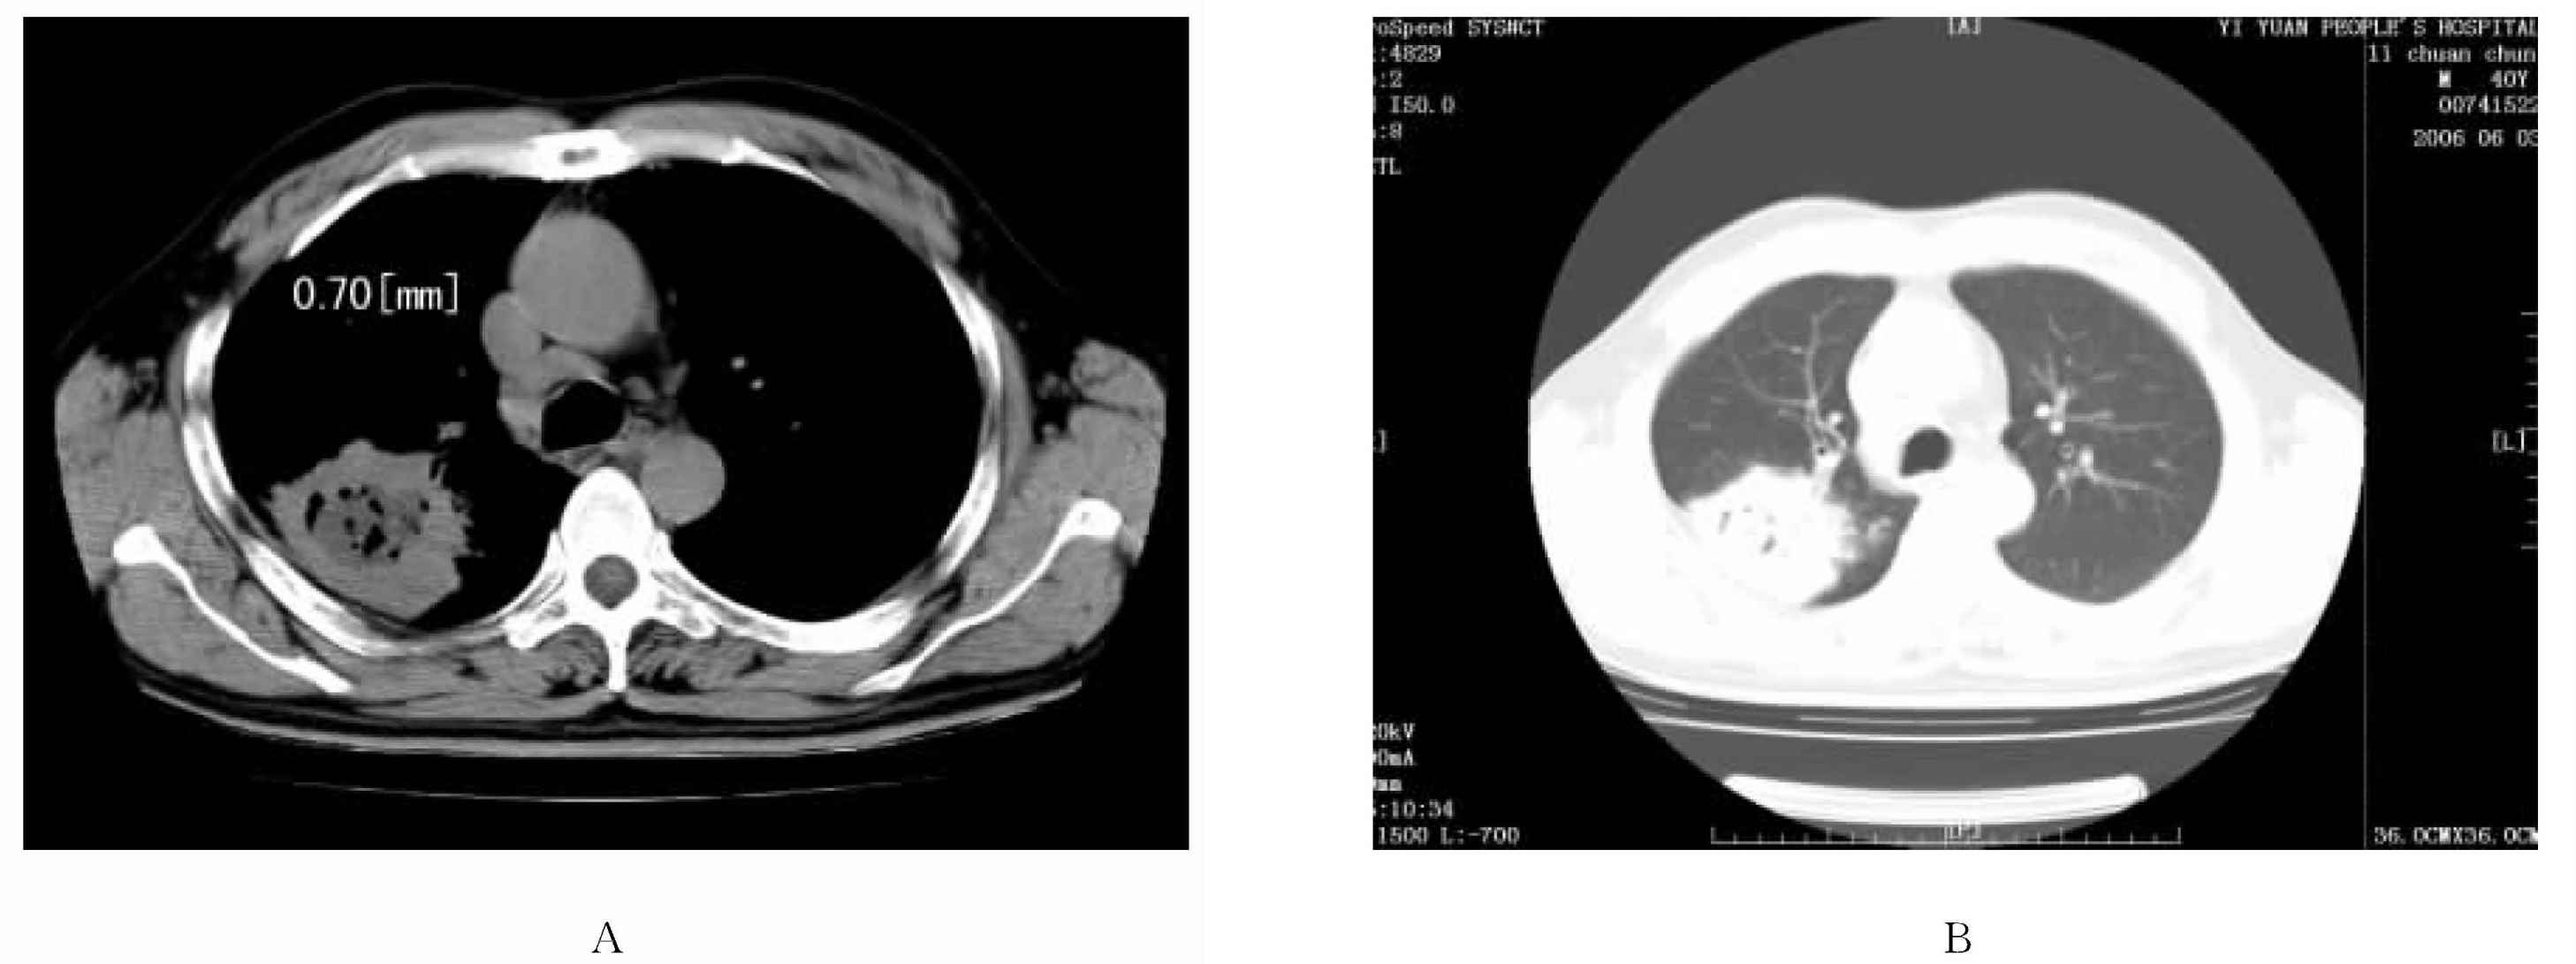
\includegraphics[width=.7\textwidth,height=\textheight,keepaspectratio]{./images/Image00205.jpg}
 \captionsetup{justification=centering}
 \caption{肺脓肿\\{\small A、B为同一患者,右上叶大片实变区内有低密度坏死区}}
 \label{fig9-20}
  \end{figure} 

\subsection{慢性肺脓肿}

急性肺脓肿迁延不愈(有学者认为3个月以上)发展到慢性阶段,即形成慢性肺脓肿。

\textbf{【病理】}
其主要病理改变为慢性肺脓肿空洞的形成,以及外周炎症逐渐吸收而纤维组织增生形成假包膜。炎症可经支气管播散到其他肺叶或肺段。或因引流支气管的阻塞而形成张力性空洞,脓液穿破洞壁向邻近肺段蔓延,形成与原来脓肿有窦道相通的多房性脓肿。也可因脓肿贴近叶间胸膜而向邻近肺叶穿破蔓延。病变区可产生支扩。

\textbf{【临床表现】}
大多数病人表现为急性肺脓肿迁延不愈,有慢性咳嗽、咳脓痰或脓血痰,体质消耗,呈慢性中毒症状,并可能有杵状指(趾)。

\textbf{【CT表现】}
以纤维厚壁空洞伴肺组织纤维化为主要表现。①空洞大小、形态不一,可呈圆形、椭圆形或不规则形。②内壁、外壁的边缘清楚,可呈多房性或多叶蔓延。③洞内可有不同程度的气液平面,少数也可无液气平面。洞周可见慢性炎症、支扩、纤维化或新的播散性病灶。④胸膜改变常见,可见脓胸或广泛胸膜增厚。⑤因支气管扭曲狭窄,引流不畅,痰液黏稠呈半固体状,可使脓腔完全闭塞,即所谓闭锁空洞。影像学呈肿块状影。

\subsection{血源性肺脓肿}

本病又称为血行迁徙性肺脓肿,多为疖、痈、化脓性骨髓炎、细菌性心内膜炎等感染灶引起脓毒败血症或输液插管时污染造成感染性栓子,经血流至肺所致。

\textbf{【病理】}
细菌栓子经血流到肺后,栓塞于肺部小动脉,所以病灶多位于肺脏表面近胸膜处,形成多个出血性水肿实变区。有些病变区有坏死而形成空洞。炎症也可累及细支气管黏膜上皮形成溃疡,进而侵及支气管周围演变为脓肿,还可形成肺气囊,亦可侵及胸膜或破入胸膜腔。

\textbf{【临床表现】}
患者往往先有其他部位的急性感染症状。也可无明显的局部感染症状而出现高热、寒颤、皮疹等。继之有咳嗽、咯痰、胸痛等呼吸道症状。

\textbf{【CT表现】}
多表现为两肺或一肺多发病灶。多为两肺多发性片状或结节状高密度灶,结节大小不一,多0.5~4cm大小;有些结节中间坏死液化而密度减低,较大的结节增强扫描可见环状强化;有些则出现空洞,出现透亮区或液气平面。可有肺气囊形成或伴有肺门、纵隔淋巴结增大。亦可有胸膜病变,或形成肺气囊后向胸膜面穿破而形成脓气胸。少见的表现为两肺比较密布的粟粒状高密度灶,也有极少数表现为单个病灶。

\subsection{肺坏疽}

本病又称为坏疽性肺脓肿,是由于毒力很强的感染侵犯肺血管,形成脓毒栓子导致肺组织非常急性的缺血性坏死所致。

\textbf{【病因病理】}
可造成肺坏疽的致病菌有金黄色葡萄球菌、链球菌、克雷白杆菌、流感嗜血杆菌、毛霉菌和曲霉菌等。它与肺脓肿的不同之处是一个遭受坏死的肺区与有生命的肺组织分离,并在空洞内形成一个无生命力的软组织肿块。

\textbf{【影像学表现】}
其影像学特征是一个偏心性透明区包围着一个肿块,类似于空洞内的霉菌球。CT有助于显示空洞内肿块。

结合病史和临床可鉴别。肺坏疽常需手术治疗,故早期诊断甚为重要。

\section{肺结核}

\subsection{概论}

\subsubsection{原发性、继发性、先天性肺结核的概念}

1.原发性肺结核:机体初次受结核杆菌感染后所发生的肺结核称为原发性肺结核。其肺部原发灶、局部淋巴管炎和所属淋巴结炎三者综合起来称为原发综合征。原发综合征的原发灶和淋巴结病变的程度可不一致。

原发性肺结核根据其病理演变过程可分为原发综合征和支气管淋巴结结核。原发性肺结核大多趋向愈合,尤其是5~12岁的儿童预后良好。

2.继发性肺结核:机体再次感染结核杆菌时所发生的肺结核称为继发性肺结核。

3.先天性肺结核:是妊娠期间或生产过程中由感染了结核杆菌的母亲传染给胎儿所致的肺结核。

\subsubsection{初次和再次感染肺结核的机体反应}

当结核杆菌侵入肺组织后,在肺内产生的病理演变一般取决于结核菌的数量、毒力、机体的抵抗力和对结核菌的过敏反应。

1.初次感染结核菌时,由于机体缺乏免疫力,肺部病灶进展较快,易随着淋巴管和血管在胸部乃至全身器官扩散,因此肺门、纵隔淋巴结增大和粟粒性结核较为多见。但是由于过敏反应低,肺部病灶的局部坏死液化较少,所以空洞较为少见。

2.当肺部再次感染结核菌时,由于过敏反应的增强,使肺部病灶易于产生坏死及形成空洞。但由于免疫力的增高,使病灶易被纤维组织所包围和修复,发展趋向局限。即使病灶广泛,肺门和纵隔淋巴结通常无增大,粟粒性结核亦较少见。

\subsubsection{肺结核病灶的病理演变过程}

结核杆菌侵入肺组织后最初产生的渗出性炎性病灶,系由炎性细胞和渗出液充盈肺泡和细支气管所造成的。渗出性病灶如早期不吸收,很快即产生结核结节,形成结核性肉芽组织,成为增殖性病灶,并常发生不同程度的坏死即干酪样改变。干酪样改变易于产生液化而形成空洞,并沿着支气管播散。渗出性病灶如迅速发展或相互融合而干酪化即形成干酪性肺炎。结核病变也可经淋巴和血行播散。这是结核病变的进展和恶化过程。

肺结核的愈合方式为吸收消散、纤维化和钙化。渗出性病灶可以自行缓慢地吸收或经治疗后很快地吸收,但较一般肺炎慢,并可残留少许纤维病变。结核性肉芽组织即增殖性病灶须经纤维化,而干酪性病灶大都须经钙化才能愈合。空洞的愈合则须经关闭、纤维化和钙化方能完成。这是渗出、增殖、干酪性病灶、空洞好转和愈合的一般规律。

由于抗结核药物的应用,渗出性病灶可以完全吸收,增殖性病灶亦可部分吸收,空洞则可以开放地愈合。必须指出,结核病灶的好转和恶化不一定单纯进行,可以有反复曲折,在好转和愈合过程中可以有恶化。

\subsubsection{肺结核的基本病变及其CT表现}

肺结核的基本病变有6种:①渗出性病灶;②增殖性病灶;③干酪性病灶;④结核性空洞;⑤纤维性病灶;⑥钙化。其中,渗出性病变和增殖性病变为肺结核的基本病理改变,其他为其病理演变的改变。在病理上,它们大多由以上不同成分的改变所组成,但以一种病变为主。如渗出性病灶,在进行影像学检查时大都有不同程度的增殖性改变,其内可见多个小点状或小结节状更高密度影。

\textbf{【CT表现】}

1.结核渗出性病灶

(1)结节状模糊阴影:代表腺泡或肺小叶的实变。病灶边缘模糊,常为多发,以两肺上叶常见。

(2)融合性实变:常为分散结节灶融合而成,呈不规则片状高密度灶,密度不甚均匀,常有支气管充气征。在HRCT上常显示小叶中心区密度增高的结节或片状影,小叶内支气管、血管壁增厚呈葡萄串样为典型表现。

2.结核增殖性病灶

渗出性病灶演变为增殖性病灶后,病变一般都缩小而局限,且密度增高,边缘清楚。这种病灶由肺泡中产生的肉芽组织即结核结节所形成,周围环绕着正常肺泡。总之,增殖性病灶影像学表现为边缘清楚的高密度影。

3.结核干酪性病灶

(1)颗粒状干酪病灶:这种病灶大多随着较多的结核杆菌经支气管或血行播散而产生。直径一般在5mm左右,常为多发。影像学表现为散在的密度较高而轮廓模糊的颗粒状阴影,如多而密集可有融合表现。

(2)结节状或团状干酪病灶:结节状干酪病灶多由渗出、增殖性病灶产生较多的干酪改变所引起,也可由几个较小的干酪病灶融合而成。直径多在1cm以上,甚至达3~4cm或更大。由于发展缓慢,在其边缘产生纤维增生,可形成一层较薄的纤维包膜,如果病灶直径>2cm即称结核球。影像学表现为直径≥1cm的结节状或团状影,密度一般较高,轮廓较为清楚,有时可见薄层包膜,其内有时可见液化。

(3)干酪性肺炎:大多由大片渗出性结核性病变很快产生干酪化所致,有时也可由多个小的干酪性病灶融合而成。干酪性肺炎的范围较大,可涉及一个整叶,至少涉及一个肺段。影像学表现为肺段或肺叶的致密实变,其内有虫蚀样空洞。小叶性干酪性肺炎呈密度较高的支气管肺炎样改变,并可融合呈大片状、团块状。

4.结核性空洞

结核病灶的空洞是由于病灶内组织坏死液化并经引流支气管排出,空气进入坏死腔内所形成。结核空洞可多发,也可单发。根据其形成的病理基础和影像学形态,其分类和影像学表现见表\ref{tab9-5}。

\begin{longtable}{c}
  \caption{结核性空洞的分类及影像学表现}
  \label{tab9-5}\\
  \endfirsthead
  \caption[]{结核性空洞的分类及影像学表现}
  \endhead
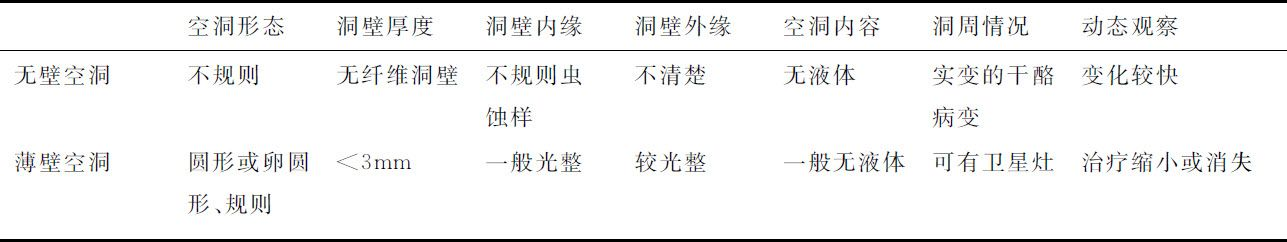
\includegraphics[width=\textwidth,height=\textheight,keepaspectratio]{./images/Image00206.jpg}\\
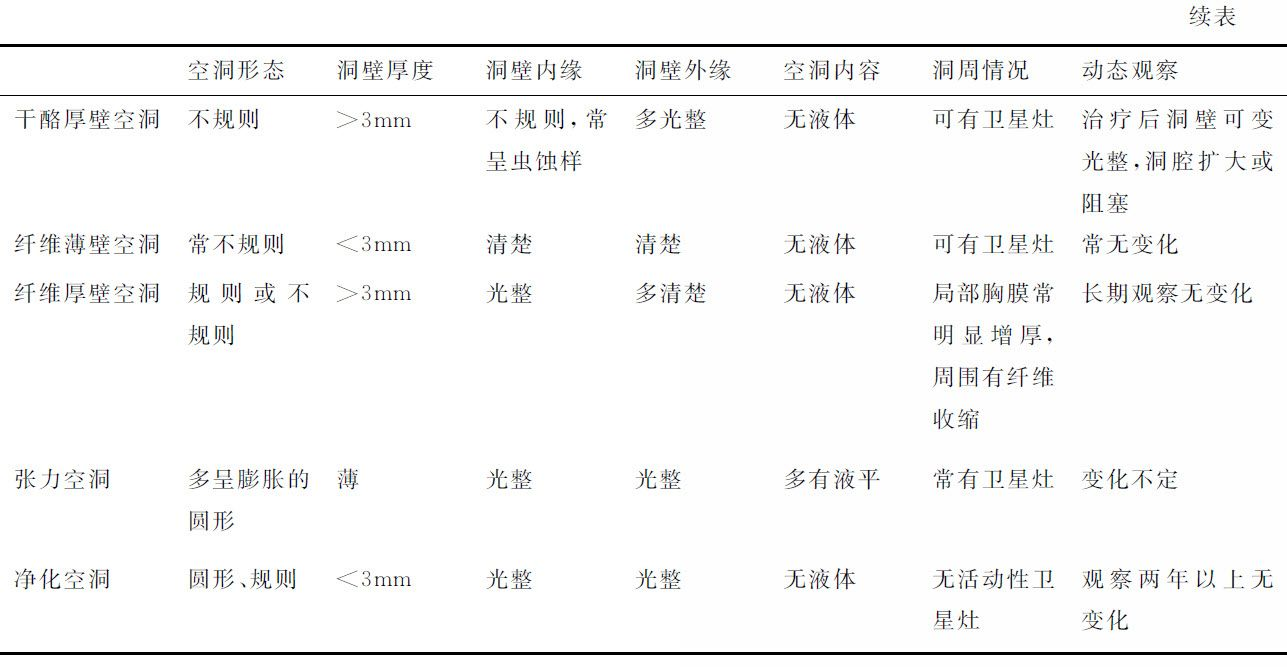
\includegraphics[width=\textwidth,height=\textheight,keepaspectratio]{./images/Image00207.jpg}
\end{longtable}



5.结核纤维化病灶

结核纤维化病灶大多由增殖性病灶愈合而成。根据其形态可分为以下5类:

(1)颗粒状纤维病灶:是由较小的增殖灶纤维化而成。表现为3~4mm左右的颗粒状高密度灶,界限清楚,边缘可光整或稍不整齐。

(2)结节状纤维病灶:是较大的增殖性病灶,从边缘开始纤维化,逐渐向内进展而形成。表现为边缘锐利、密度较高的圆形或卵圆形结节状影,大小在1cm左右。需与干酪病灶鉴别,如边缘光整,为一层薄膜线所包围,提示为干酪灶;如边缘锐利,但有不规则收缩牵拉现象,则提示为纤维化病灶。

(3)星形或斑片状纤维病灶:表现为有多个尖突的星形高密度灶或小斑片状的不规则高密度灶。

(4)索条状纤维病灶:为肺实质性或间质性,大多代表已完全纤维化的病灶。沿索条状影或在其附近可见散在的小结节状高密度灶提示为结核,否则难与一般肺炎的纤维化改变相鉴别。

(5)大片弥漫性纤维化(肺硬变):类似不张,密度常不均,可见残存的结核病灶。

6.钙化病灶

大多在干酪性病灶的愈合过程中产生。其形态多样,如小点状、颗粒状、较大的结节状、团块状、环状、弥漫粟粒状等,可位于整个结核灶的中心或边缘、局限或散在、弥漫。

\subsubsection{肺结核的分型}

肺结核分为以下5型:①原发型肺结核:包括原发综合征和胸内淋巴结结核;②血行播散型肺结核:包括急性粟粒性肺结核和慢性血行播散性肺结核;③浸润型肺结核:包括肺尖、锁骨下等处的结核、干酪性肺炎、结核球;④慢性纤维空洞型肺结核;⑤结核性胸膜炎。

\subsection{原发型肺结核}

原发型肺结核(包括原发综合征和支气管淋巴结结核)多见于儿童,青年约占20%,成人约占8%~10%。

\textbf{【病理】}
结核杆菌侵入肺组织后,在肺泡内产生急性渗出性改变,其大小多在0.5~2.0cm之间,这种局限性实变称为原发病灶。原发灶的结核杆菌通过局部淋巴管侵入病灶所属的1个或数个支气管肺部、肺门以及支气管周围的淋巴结,导致局部淋巴管和淋巴结炎。其肺部原发灶、局部淋巴管炎和所属淋巴结炎三者综合起来称为原发综合征。在结核杆菌感染后2~6周,随着结核杆菌的繁殖和死亡,机体出现对结核菌体蛋白及其代谢产物的过敏反应,在原发灶和淋巴结周围发生明显的炎性渗出即病灶周围炎,使原发病灶扩大,甚至涉及整个肺叶。进而原发灶可干酪坏死和形成结核性肉芽肿,然后原发灶局限、纤维化、钙化而愈合。

原发型肺结核大多趋向愈合,尤其5~12岁儿童预后良好。可有以下恶化途径:①原发空洞形成;②淋巴性播散:淋巴结增大或引流入上腔静脉,引起淋巴血行播散,亦可为离心性沿淋巴管播散至胸膜;③支气管播散:可为广泛的小叶性病灶,亦可融合成节段性或大叶性,但密度不均,内有空洞;④血行播散。

\textbf{【临床表现】}
低热、咳嗽、盗汗和消瘦为主要的临床症状,但通常症状和体征缺乏特征性。有些可无任何症状,体检偶然发现。在其病程中症状如有明显加重则提示病变有恶化或有并发症发生。

\textbf{【影像学表现】}

\subsubsection{原发综合征}

本病有以下4种表现:①原发病灶及病灶周围炎:好发于上叶的下部和下叶的上部,靠近胸膜下。以右肺多见,上叶多于下叶。原发病灶大小、多少不一。机体产生过敏反应后原发灶产生病灶周围炎时,表现为大片絮状高密度灶,可累及一个肺段甚至整个肺叶,整个肺叶受累以右中叶多见。偶见原发灶在絮状高密度灶内呈更高密度影。病灶周围炎的吸收一般较缓慢,小区域的炎性浸润至少需要3个月才能吸收,大面积者吸收更慢。随着病灶周围炎的吸收,愈合中的原发灶可显示为界限清楚、密度较高的增殖性或已部分钙化的病灶。②淋巴管炎:表现为一条或数条模糊的索条状高密度影,自原发灶伸向肺门。③淋巴结炎:增大的淋巴结多位于同侧肺门,但也可通过淋巴引流累及对侧肺门。④胸膜改变:可有局限性增厚甚至胸腔积液。

原发病灶与淋巴结病变的程度和愈合过程并不完全一致。原发病灶、淋巴管炎及肺门淋巴结增大如同时显示,则形成原发综合征的典型表现即二极期。

\subsubsection{胸内淋巴结结核}

肺内原发灶已吸收或纤维化,或原发灶较小以致难以显示或确认,而增大的淋巴结在继续进展中,肺门和(或)纵隔淋巴结增大明显。目前典型的原发综合征比较少见,原发性肺结核以胸内淋巴结结核为常见。既可见于儿童,也可见于成人。

1.影像学分型:分为2型。①炎症型:淋巴结增大伴周围肺组织渗出性炎性浸润;②结节型:淋巴结周围炎吸收后,在淋巴结周围有一层结缔组织包围(图\ref{fig9-21})。总之,两者均表现为肺门或气管旁淋巴结增大,前者边缘模糊,后者边缘清晰。增大淋巴结常位于肺门与右气管旁,也可累及隆突下与主-肺动脉窗淋巴结,多为单侧发病。

\begin{figure}[!htbp]
 \centering
 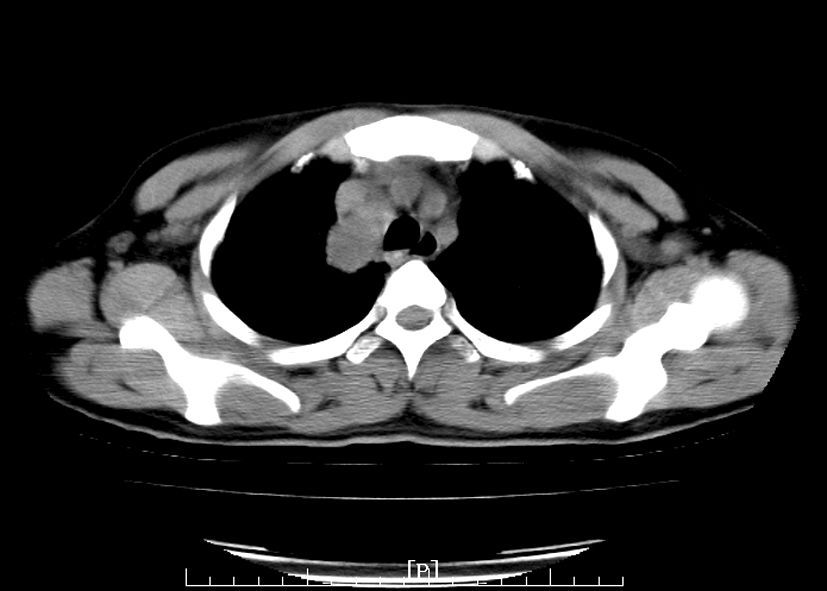
\includegraphics[width=.7\textwidth,height=\textheight,keepaspectratio]{./images/Image00208.jpg}
 \captionsetup{justification=centering}
 \caption{胸内淋巴结结核\\{\small 右侧气管旁有显著增大淋巴结,界限欠清晰}}
 \label{fig9-21}
  \end{figure} 

2.增强扫描:增强扫描易于显示增大淋巴结,尤其是>2cm的淋巴结。其强化方式为:①明显的周边环状强化:强化环的数目、大小不等,环厚2~4mm,环中央不强化。强化环为淋巴结包膜及其周围富血管的炎症反应所致。②不均匀强化和均匀强化:前者代表淋巴结内肉芽组织和干酪坏死并存,后者代表均匀肉芽组织增生。③间隔状强化:见于多个干酪坏死淋巴结相互融合。以中央出现不强化的低密度,周围出现环状强化为特征。国内有学者报道2例不典型者,表现为多组淋巴结受累,显著坏死液化并相互融合成较大的囊状水样密度病灶(但壁较厚0.8~1.0cm),且侵及周围组织结构和胸膜(双侧胸腔积液)。

中央不强化的低密度为干酪坏死和液化,是活动性的可靠标志。而钙化或淋巴结密度均匀,既可见于活动性病变,也可见于非活动性病变。还有文献认为非活动性者淋巴结呈均匀状、无边缘强化,83%的淋巴结内有钙化,47%肺内有陈旧性结核灶。结核性淋巴结炎穿破包膜可引起纵隔炎,并可使气管、上腔静脉、食管及心包受侵、受压。

\textbf{【鉴别诊断】}

1.非结核性肺炎:细菌或病毒感染所引起的片状肺炎与原发性肺结核的原发灶相似,且非结核性肺炎亦可造成肺门淋巴结增大。所以两者不易鉴别,主要依靠临床检查。如在片状高密度灶内见到斑点状更高密度灶,提示原发性肺结核的可能。

2.恶性淋巴瘤:本病生长迅速,易融合成团,病变以纵隔为主,且多为两侧性,无钙化,可有肺内浸润,与结核有别。

3.与胸内淋巴结结核类似的环状强化也可见于:非典型性分支杆菌感染、淋巴瘤、转移瘤(尤其是睾丸癌的转移),其他疾病如Whipple病(肠源性脂肪代谢障碍)及Crohn病。但有学者认为结核性坏死性淋巴结炎呈边缘很厚的强化且不均匀,而肿瘤转移的淋巴结呈相对薄壁的环形强化。还有报道,干酪坏死区CT值约40Hu,平扫与未坏死区密度相近,而鳞癌转移和恶性淋巴瘤之液化坏死区密度更低CT值为8~15Hu。

\subsection{急性粟粒性肺结核}

本病是由于大量结核杆菌一次侵入血循环所引起。以在原发性肺结核中较多见,其结核杆菌进入血流的途径有以下几种:①在初次感染的早期,结核杆菌经过淋巴道进入血循环,形成早期血行播散;②干酪样原发病灶直接侵蚀邻近的肺动脉或肺静脉;③干酪样的淋巴结引起淋巴血行播散。继发性肺结核中则多由其他部位的结核灶破入静脉所致。

\textbf{【病理】}
病灶弥漫性均匀分布于两肺。根据病菌的数量和毒力,以及机体的抵抗力,病变随时间的演变可以增殖为主或形成渗出干酪性病灶。

\textbf{【临床表现】}
起病急剧,症状严重,持续发热、寒颤、咳嗽、呼吸困难、紫绀甚至头痛、昏迷。

\textbf{【HRCT表现】}
①微结节:96%可见到。结节在两肺内呈均匀、弥漫随机分布,并可达胸膜下及叶间裂。大小约1~3mm,少数可达5mm,且大小、密度均匀。病灶边缘大多清楚,少部分模糊(图\ref{fig9-22})。经2~6个月治疗可完全吸收(不留痕迹)或钙化。②磨玻璃状影:92%可见到。呈斑片状,随机分布,为显微镜下才能看到的小干酪性肉芽肿,绝大多数同时见到微结节。③其他:可有小叶内间隔增厚和小叶内网状影,亦可有纵隔淋巴结增大和支气管源性播散灶。此外,应该注意急性粟粒型肺结核可能引起小叶间隔结节,并呈串珠状表现,但一般不引起肺门部的支气管血管束结节,有别于癌性淋巴管炎(转移瘤结节相对较大且大小不均)、结节病等。

\begin{figure}[!htbp]
 \centering
 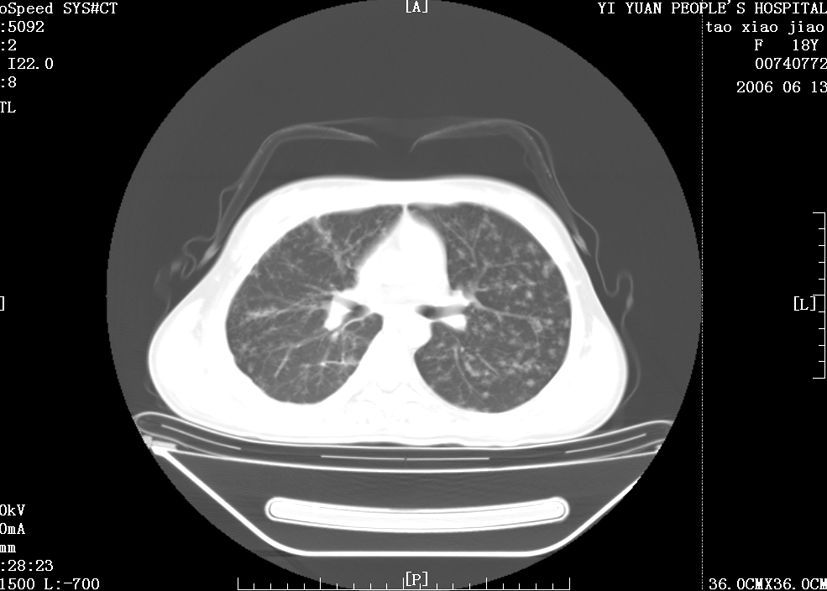
\includegraphics[width=.7\textwidth,height=\textheight,keepaspectratio]{./images/Image00209.jpg}
 \captionsetup{justification=centering}
 \caption{急性粟粒性肺结核\\{\small 两肺弥漫性分布有许多粟粒状结节,大小、密度、分布较均匀。病灶边缘大多清楚,少部分模糊}}
 \label{fig9-22}
  \end{figure} 

急性粟粒性肺结核出现气肿泡均发生在粟粒病灶增大呈渗出变化的过程中。病灶增大渗出时,对呼吸性细支气管压迫或阻塞,使之呈活瓣作用,致使远端肺泡空气潴留而形成气肿泡或肺气囊。气肿泡或肺气囊破入胸腔形成气胸,亦可形成间质性肺气肿进而形成气胸。

\textbf{【鉴别诊断】}

1.血行播散型转移瘤:大小不一致、分布不均匀,特别是下肺部较上肺部病灶多而大,较有意义。淋巴血行转移瘤可见支气管血管束增粗、毛糙且合并结节。急性粟粒性肺结核大小多为1~3mm(少数可达5mm),且大小均匀;转移瘤大小不均,结节相对较大。

此外,急性粟粒性肺结核可能引起小叶间隔结节,呈串珠状表现,但一般不引起肺门部的支气管血管束结节,有别于癌性淋巴管炎、结节病等。

2.肺血吸虫病:早期可呈两肺弥漫的粟粒状结节,密度一般较淡、边缘较模糊,且分布不均,以两中下肺多见,还可出现片状、絮状高密度灶。结合疫水接触史和血液中嗜酸粒细胞的增多可以做出诊断。

\subsection{慢性血行播散性肺结核}

本病是由于较少量的结核杆菌在较长时间内屡次侵入血循环所造成。其播散的来源可由原来的肺结核灶或其他部位的结核灶侵入静脉所致。

\textbf{【病理】}
一次较少量的结核杆菌所引起的肺血行播散灶分布范围较小,多见于肺尖部,有时可限于一侧,呈粟粒状。当初次播散的病灶趋向愈合时,再次血行播散在两肺上部又出现新的病灶,范围向下伸展。经长期反复播散,使病灶的数目增多、范围增大。新老病灶同时存在或混杂存在,有的可相互融合。

\textbf{【临床表现】}
早期多无明显症状。当反复的血行播散,可出现明显的结核病症状。

\textbf{【CT表现】}
表现为大小不一的多发结节灶,从粟粒样至直径1cm左右。密度不一,从渗出、增殖灶到钙化灶。形态不一且分布不均,老的硬结、钙化灶大多位于肺尖和锁骨下,新的渗出、增殖灶大多位于下方。亦可有病灶融合、空洞形成、支气管播散。总之,其所谓分布、大小、密度三不均为其特点。

\textbf{【鉴别诊断】}

1.细支气管肺泡癌:其弥漫型可能是其结节型和浸润型通过淋巴、血行或支气管播散而致。表现为结节大小不一,在两肺分布不对称(两下肺为著)和不均匀(在一处较密集而另一处较松散)。结节病灶的融合,以及融合病灶的支气管充气征是与粟粒性肺结核的主要鉴别点;亦与亚急性慢性血行播散性肺结核由肺尖向下的老、中、青“三辈”病灶,不难鉴别。

2.支气管源性播散性肺结核:血行播散型肺结核不论急性或亚急性随血液动力学的因素,肺尖首先受侵袭,痰菌常阴性。而支气管源性播散性肺结核不论发生在上叶或下叶,均自肺门向邻近支气管播散;结节影常较大而毛糙,大小不一;痰菌可阳性;HRCT呈位于小叶中心的小气道结节和“树枝发芽”征。此外,亦应注意与其他经支气管播散的感染(如支气管肺炎早期)、小气道疾病合并感染(如感染性细支气管炎)相鉴别。

\subsection{浸润型肺结核}

本病是继发性肺结核中最常见的类型,多见于成人。结核菌可来自肺部的原发性肺结核灶,也可再从外界吸入肺部。

\textbf{【病理】}
关于其机体反应和病理演变详见本节概述。浸润性结核灶最初通常在锁骨上下形成渗出性病灶,如不顺利吸收即形成结核结节,且常伴有干酪性改变。干酪灶可液化并经气道播散到其他区域,严重者可以渗出和干酪为主,形成急性干酪性肺炎。浸润型肺结核如不经适当治疗可形成空洞和支气管播散。病变好转,可经纤维化、钙化等方式愈合。在慢性病例中可多种病灶共存。

\textbf{【临床表现】}
多种多样,有的患者早期无症状或症状轻微,体检偶然发现。常见症状为:①全身中毒症状:如发热(一般不高)、面部潮红、夜间盗汗、脉搏加速、身感不适、疲乏、食欲不振和消瘦等。②胸部局部症状:如咳嗽、咳痰和咯血等,涉及胸膜有胸痛。血液检查可见ESR增快,白细胞分类可出现单核、淋巴细胞增多。

\textbf{【CT表现】}

\subsubsection{典型的活动性肺结核}

表现为发生在常见和非常见部位的肺实变影,伴有局限或广泛的支气管播散灶(图\ref{fig9-23}A)。在HRCT上见到2~4mm的小叶中心结节或分支线样结构即“树芽征”(68.9%)和5~8mm边缘模糊的结节影(69%)均应初诊为活动性肺结核;同时出现钙化或纤维化征象,则强烈支持肺结核的诊断。此外还有支气管壁增厚、磨玻璃样影、空洞、小叶间隔增厚、液体支气管征象等均支持为活动性肺结核。

1.关于肺实变影:是指在肺窗上及纵隔窗上均能看到的软组织密度影,而且纵隔窗其面积不小于肺窗所见的50%。约44%的活动性肺结核有肺实变。国外有学者发现在段和叶的实变中,结核性者68.9%有液体支气管征。

液体支气管征表现为实变区中宽1~2mm的分支状、线状或圆形(HRCT多呈圆形或卵圆形)近水样低密度影,为小气道结核性支气管炎的表现。

2.关于肺内支气管播散:肺结核在肺内蔓延进展的途径包括局部浸润、支气管播散、淋巴播散和血行播散。支气管播散是继发性结核的最常见形式,在常规CT上呈沿纹理分布的斑片影。而HRCT主要表现为:①2~4mm的小叶中心结节或
“树芽征”;②5~8mm的边缘模糊的结节影,代表小叶中心的坏死性肉芽肿及其周围非特异性炎症的腺泡结节;③支气管壁增厚;④磨玻璃影。

3.关于钙化、纤维化:是结核修复、好转的表现,是非活动性肺结核的主要征象。纤维化呈不规则线状影。

\subsubsection{肺结核}

结核病灶部分或大部分已钙化,周围有纤维条索影,通常是其特征性表现。较明显的纤维化可使周围肺结构紊乱(如支气管血管束变形)并可见支气管扩张、肺容积减小、瘢痕旁肺气肿。此外,还可见纵隔淋巴结钙化、胸膜增厚、支气管壁增厚、小叶间隔增厚等。还有报道12%可见到薄壁空洞,但其他肺野内无播散灶有助于与活动性病变鉴别。

但上述改变并非完全可靠,通常要做至少6个月的观察,无改变时才能认为是非活动性或陈旧性肺结核。

\subsubsection{结核空洞及其演变}

结核空洞常位于上叶尖、后段以及下叶背(上)段。在急性或亚急性期常有厚壁,内缘多不规则,形态欠规整;至慢性期壁多薄且趋向均匀光整。除非有引流支气管阻塞一般无液平或有浅小液平。周围多有卫星病灶(图\ref{fig9-23}B)。

\begin{figure}[!htbp]
 \centering
 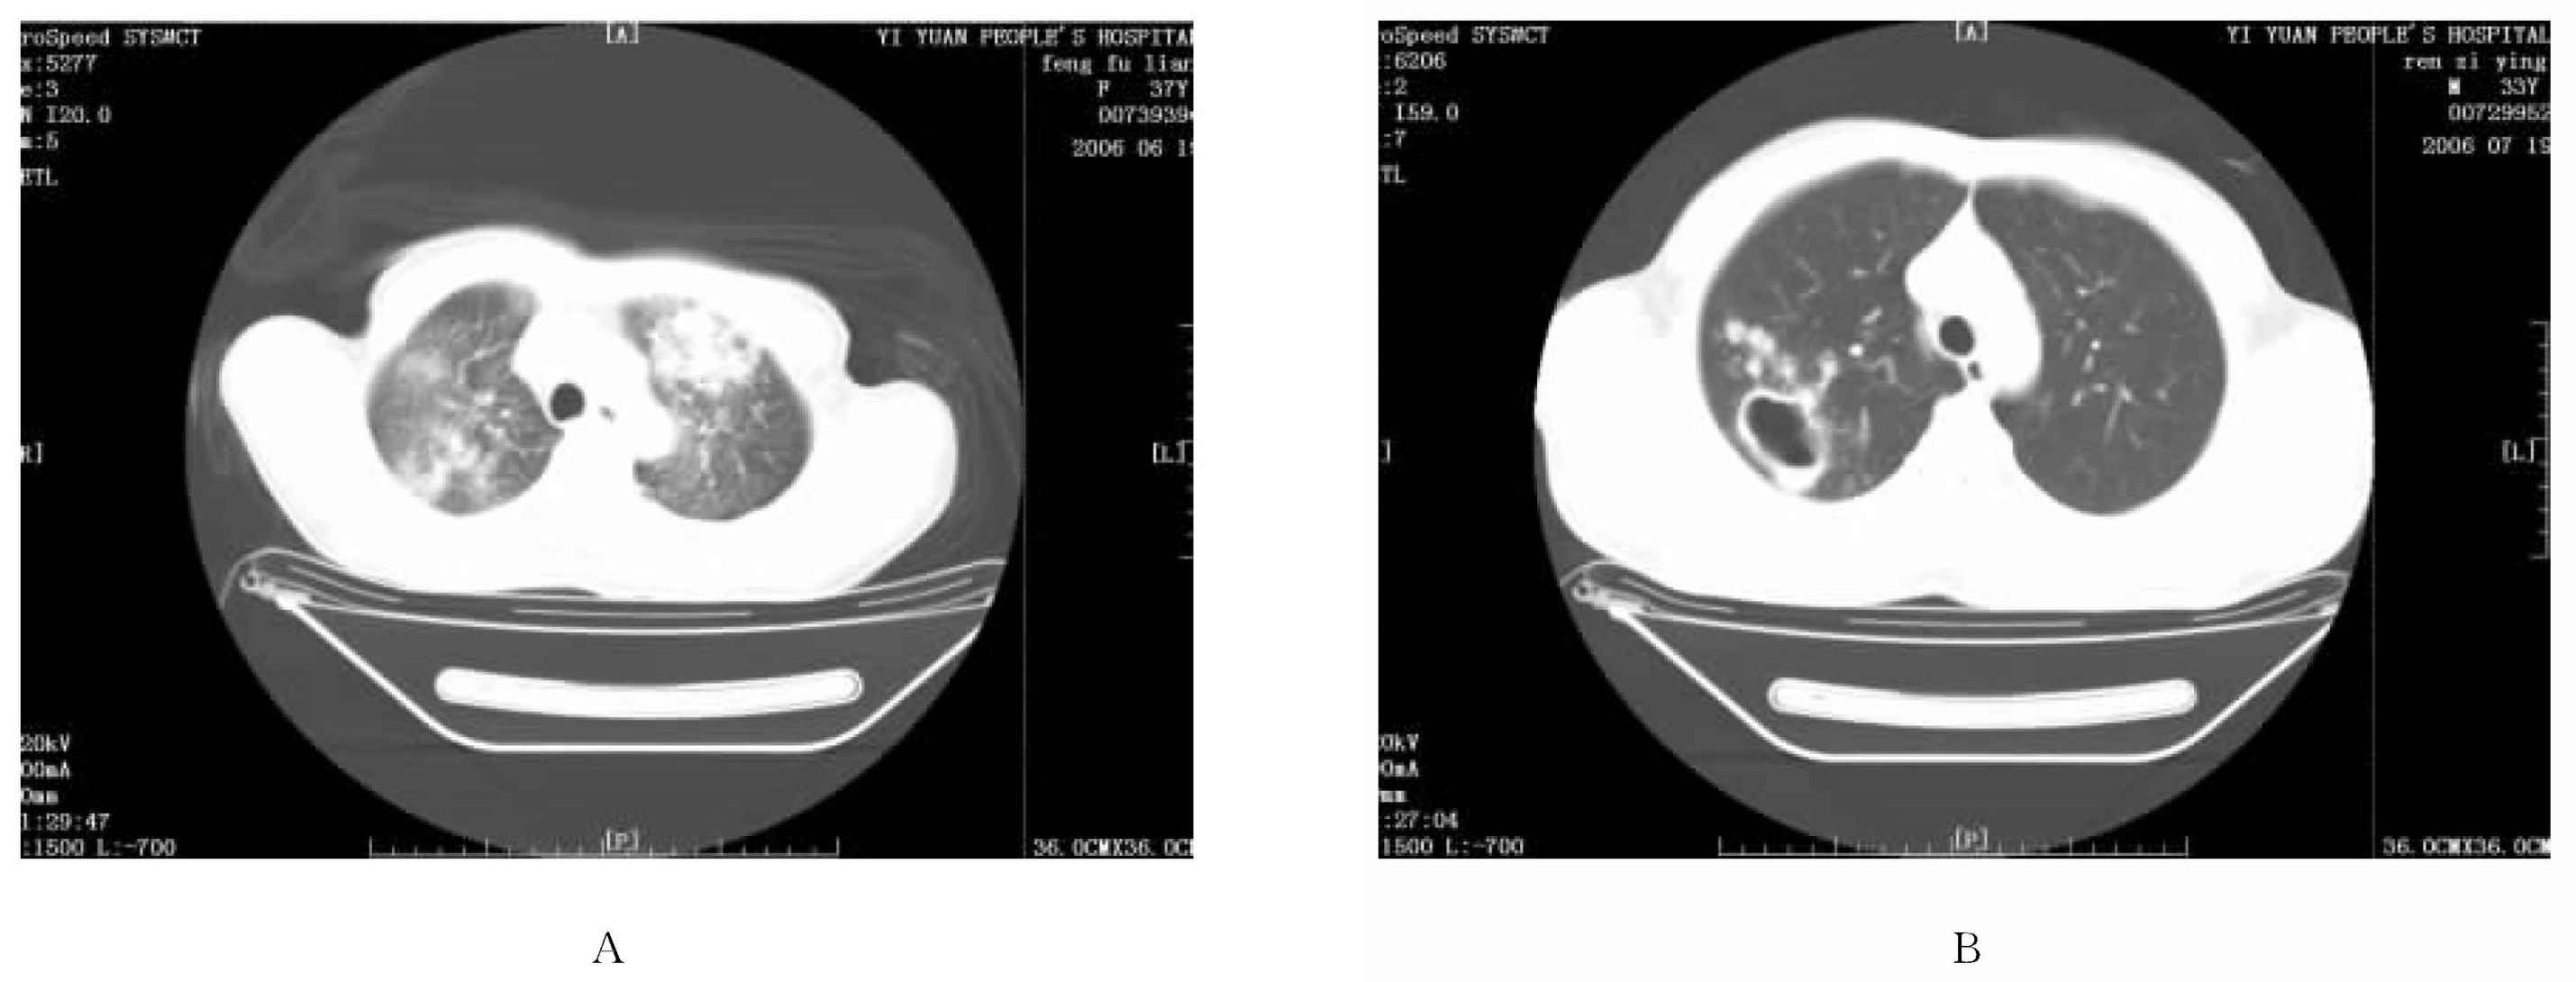
\includegraphics[width=.7\textwidth,height=\textheight,keepaspectratio]{./images/Image00210.jpg}
 \captionsetup{justification=centering}
 \caption{浸润性肺结核\\{\small A.左右肺上叶有云絮状高密度灶,密度欠均,边缘模糊,其内有斑点状更高密度灶;B.右肺上叶有薄壁空洞,其内有浅小液平,周围有多个斑点状高密度灶(卫星灶)}}
 \label{fig9-23}
  \end{figure} 

其愈合经下列几种方式。①纤维收缩:空洞中干酪样物质完全排出后,洞壁由于纤维收缩而逐渐缩小闭合,最后形成纤维瘢痕。此种愈合方式必须具备两个条件,即引流支气管必须通畅和周围肺组织必须有足够的弹性。因此,如在洞周围有较多实质性病变,则可以估计空洞不易收缩愈合。②空洞闭塞:引流支气管被阻塞,空洞被干酪样物充填而凝集,周围被纤维膜包围形成结核球。这种方式愈后差,可重新液化形成空洞。③开放性愈合:引流支气管的上皮细胞向空洞内壁生长覆盖,空洞不再排菌,这种空洞称为净化空洞。影像学表现为空洞壁薄而均匀,无张力,周围无活动性病灶。如果洞壁有局限性增厚则表示空洞尚未完全净化。

\textbf{【鉴别诊断】}

1.以渗出为主的结核需与其他肺炎,特别是肺炎支原体肺炎相鉴别,因为它们的表现相似。如在渗出灶内看到夹杂有小颗粒状或结节状更高密度灶,或在其他区域有支气管播散病灶,则应考虑为结核。支原体肺炎和其他肺炎一般吸收较快,并可完全消失或留少许瘢痕;而结核灶则吸收缓慢,并往往产生纤维化痕迹。

2.对于呈肺段、肺叶阴影的肺结核,CT即使MR也不能分辨增殖灶、干酪性病灶及慢性肺炎,但可显示其支气管扩张。此种结核与中央型肺癌的鉴别应着重于对肺段、肺叶支气管的观察。

3.非结核性分支杆菌是一种普遍存在的微生物(它不像结核那样由个人间传染,而是暴露于环境内的感染),该病的临床症状和体征多与结核病相似;病程是一种慢性、惰性的过程,X线上常可持续多年不变。在疑为肺结核甚至痰分支杆菌阳性的病例中,经长期抗结核治疗无效或有反复发作,而影像表现呈多种病变形态共存(斑片状及片状实变、空洞、纤维性病变和结节是其主要表现)并累及多个肺叶时,应考虑到该病可能,尽早做非结核性分支杆菌培养,以便确诊。

4.结核空洞与肺脓肿和肺癌空洞等的鉴别(见表\ref{tab9-6})。

\begin{table}[htbp]
\centering
\caption{结核空洞的鉴别诊断}
\label{tab9-6}
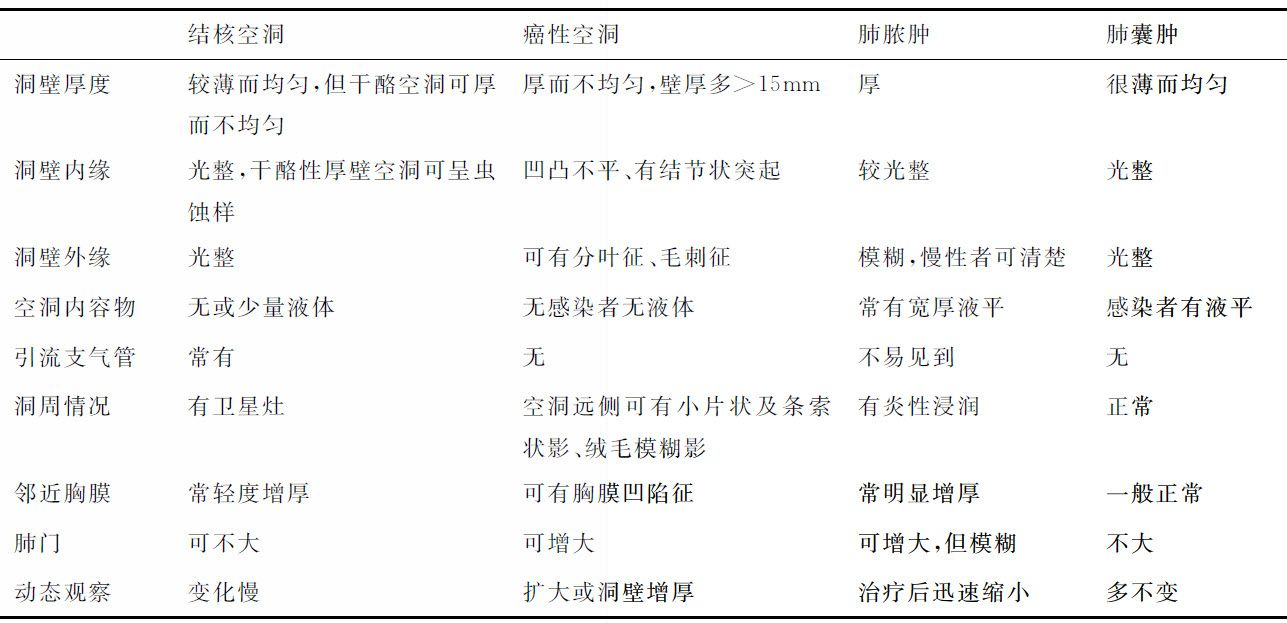
\includegraphics[width=\textwidth,height=\textheight,keepaspectratio]{./images/Image00211.jpg}
\end{table}

\subsection{结核球}

本病亦称为结核瘤,属浸润型肺结核。在我国结核球是孤立性肺结节中最常见的一种。

\textbf{【病因病理】}
结核球是被纤维组织包围的结核干酪性病变(亦可含有一定的肉芽组织),直径>2cm者称为结核球;而<2cm者称为纤维干酪结节,但亦有人仍将其称为结核球或小结核球。结核球>5cm者相当少见。

其形成方式如下:①由干酪样肺炎局限、纤维化而形成;②由纤维性肉芽组织干酪坏死所形成,往往是由几个小病灶融合而成;③由阻塞性空洞充满干酪物质所形成;④由靠近肺门的较大气管结核向外发展形成。其中第一种最为常见。

结核球包膜内层为含血管结构的结核性肉芽组织,外层为透明变性的纤维结缔组织。急性进展性结核球周围有炎性血管增生及充血反应。结核球实质部分是否有血供不能一概而论,与其病理进程密切相关。早期如果坏死不均匀或不彻底则实质应有血供。但对于陈旧性结核球由于病灶坏死彻底,包膜内层也可缺乏肉芽组织结构,病灶实质区及包膜则不可能存在血管结构。

\textbf{【临床表现】}
一般无明显临床症状和体征。追问病史可有结核史,但也可病史不清。

\textbf{【CT表现】}

1.平扫表现:①形状和大小:多为圆形、椭圆形或梨形。大小不一,直径多为0.5~4.0cm。②数目和部位:常单发,多发者少见,可发生于两肺任何部位,以两肺上叶尤以右上叶多见。③密度和轮廓:密度常不均匀而且较高,轮廓通常光滑整齐,约10%呈浅分叶状;病灶发展期边缘可模糊。④钙化:约占20%~30%,结节内有钙化是结核球的较特征性表现,可呈弧形、多层状、弥漫性斑点状、靶心样、点状、爆米花样,尤以层状钙化最具特征性。⑤卫星灶:90%有卫星病变。⑥空洞形成:空洞呈圆形、椭圆形等,裂隙样空洞和偏心性靠边缘的半月形空洞较有特征。⑦胸膜病变:多数有胸膜粘连带为本病的另一特征(图\ref{fig9-24})。

\begin{figure}[!htbp]
 \centering
 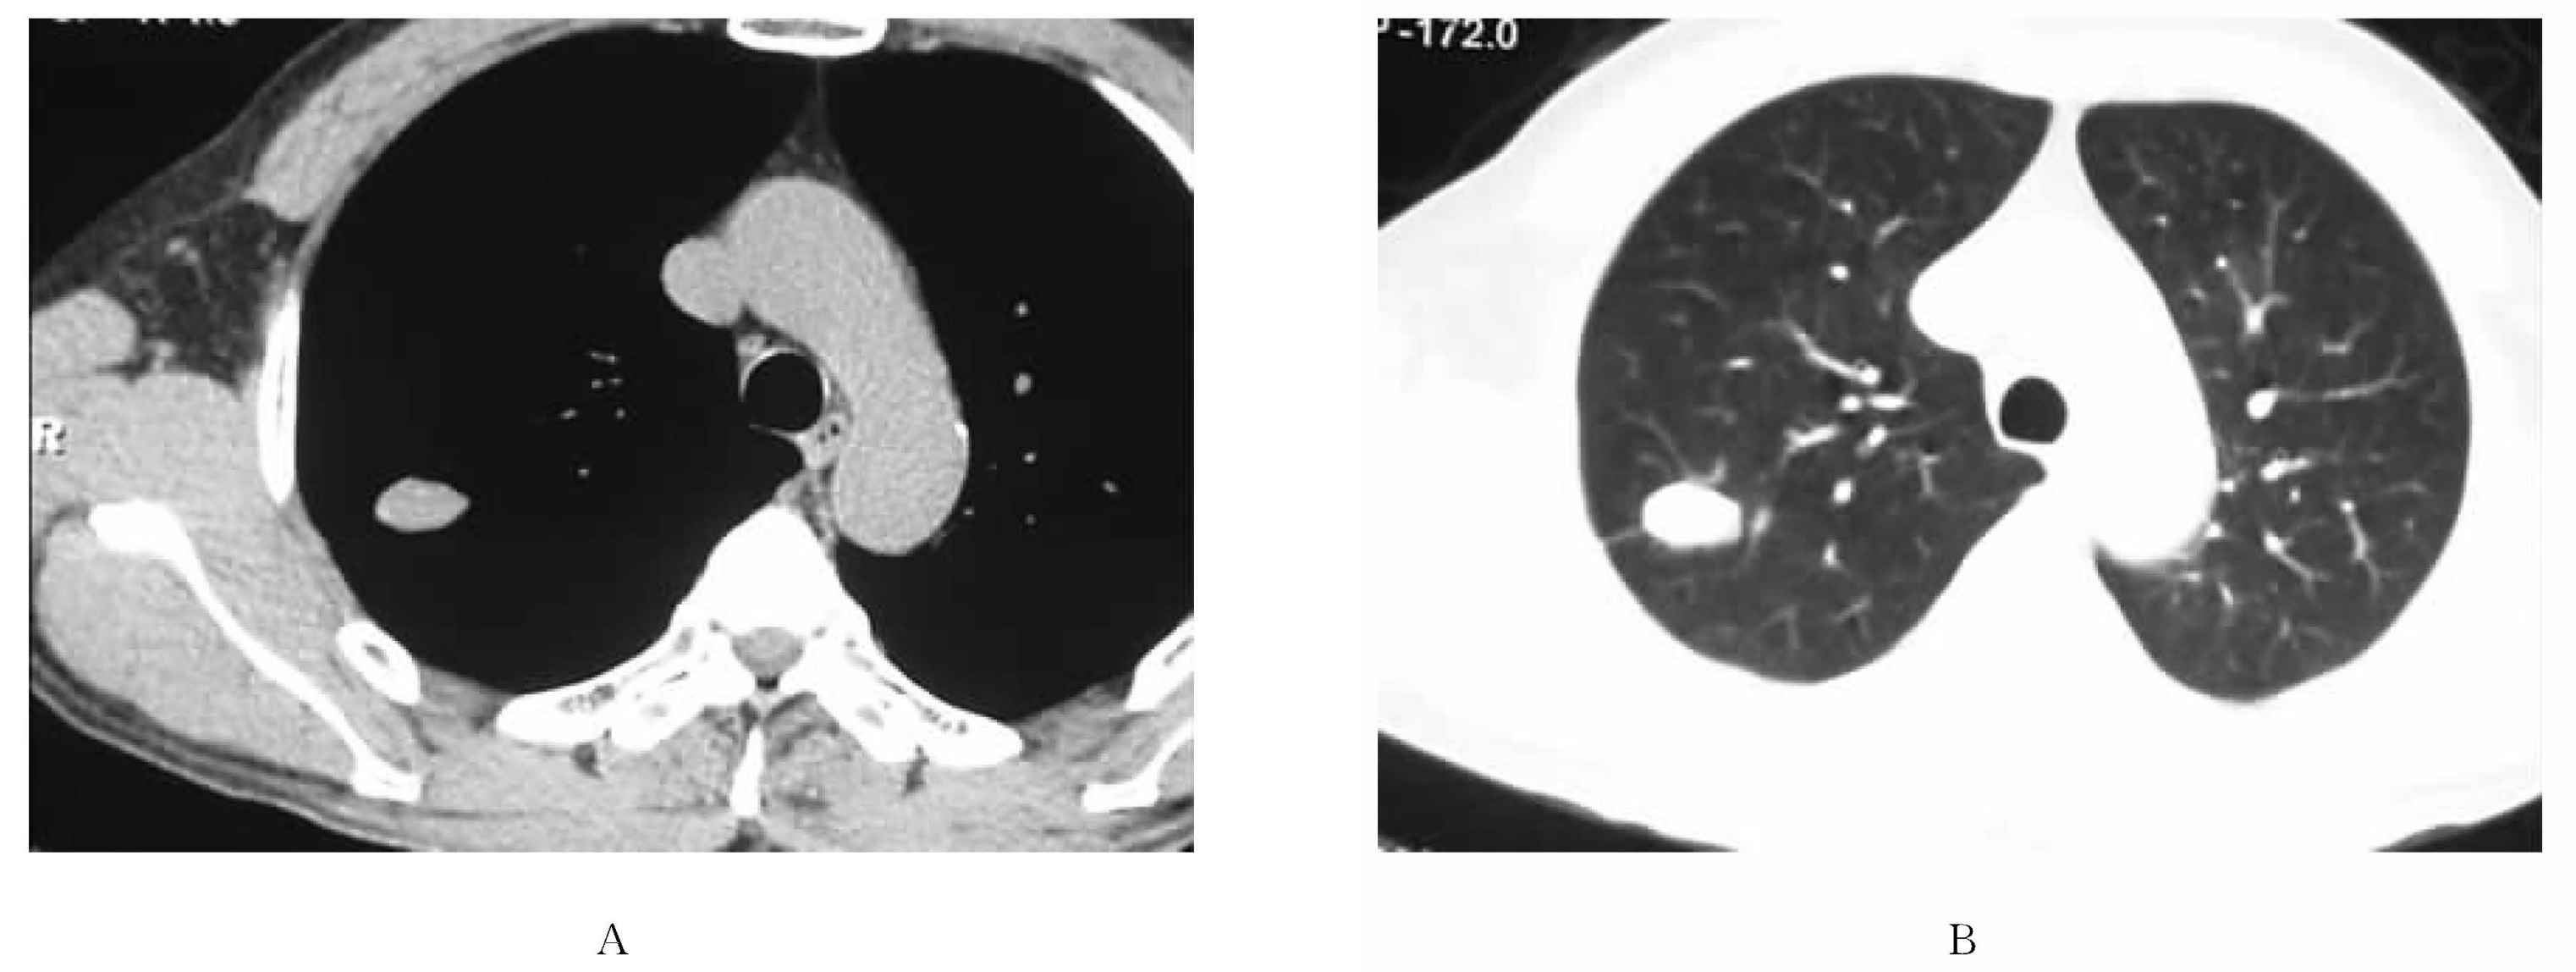
\includegraphics[width=.7\textwidth,height=\textheight,keepaspectratio]{./images/Image00212.jpg}
 \captionsetup{justification=centering}
 \caption{结核球\\{\small 右肺上叶有椭圆形高密度灶,边缘光滑,其内有多个斑点状钙化}}
 \label{fig9-24}
  \end{figure} 

2.增强表现:①CT值改变:多无明显强化,CT值增加值报道不一,如(3±6)Hu、(13.4±2.2)Hu等,仅有极少数明显强化。②形态改变:国外有报道,58%呈环形或不完全环形强化;17%为中央部弧形强化;25%呈非特异性强化。由此可见,环形或不完全环形强化是其特征。环形包膜样强化的特征说明部分结核球虽然实质无明显强化,但其纤维包膜下含有血管结构丰富的肉芽组织层是其包膜下强化的病理基础。③时间-密度曲线特征:大多数结核球(以及良性肿瘤)的时间-密度曲线上升幅度极小并维持较低的平台水平,但活动性炎症反应期结核可与其他非特异性炎性结节或球形病变一样呈逐渐上升型(有文献报道还可呈锯齿状不规则型、速升速降型)强化曲线。

\textbf{【鉴别诊断】}
①主要应与肺癌鉴别。后者有边缘分叶征、短细僵直毛刺征、空泡征、胸膜凹陷征等;增强后CT值升高可达(40±10)Hu,肺癌多为完全强化或不均匀强化,且强化曲线特征是上升到峰值后维持高水平一段时间(呈抛物线状)。②少数活动性结核球强化明显,与炎性假瘤、机化性肺炎及强化明显的错构瘤鉴别困难。

\subsection{干酪性肺炎}

本病属浸润型肺结核,见于机体抵抗力差,对结核杆菌高度过敏的病人,是由于大量结核菌经支气管侵入肺组织而迅速引起的干酪样坏死的肺结核。

\textbf{【病因病理】}
它主要来源于干酪样坏死的支气管淋巴结结核;也可来自慢性活动性结核病灶的迅速干酪样坏死后,由空洞排放大量干酪样坏死物质并经支气管播散。干酪灶液化并经气道播散到其他区域后,发生严重的渗出和干酪坏死,即形成急性干酪性肺炎。

\textbf{【临床表现】}
病情急剧恶化,引起明显的结核中毒症状。患者出现高热、寒颤、咳嗽、胸痛、呼吸困难及痰中带血。

\textbf{【影像学表现】}

1.大叶性干酪肺炎:好发于右肺上叶。整个肺叶或肺段实变,早期密度可不均匀,很快出现虫蚀样空洞,肺叶体积通常缩小。其他肺叶可见支气管播散灶。短期复查无明显变化。

2.小叶性干酪肺炎:病灶沿支气管分布,呈支气管肺炎状,以两下肺多见。病灶呈融合趋势,可有空洞。不典型者可呈团块状。病变发展迅速。

总之,干酪性肺炎的影像学诊断需密切结合临床综合诊断。

\textbf{【鉴别诊断】}
与大叶性肺炎的主要鉴别点:干酪性肺炎多见于右肺上叶,致密影的密度较高且不像大叶性肺炎那样均匀,其内有虫蚀样空洞。在同侧或对侧可见播散性肺结核灶。痰内可查到结核菌。

\subsection{慢性纤维空洞型肺结核}

本病是继发性肺结核的晚期阶段。

\textbf{【病理】}
肺组织破坏较严重,两肺上部有多发的、纤维包膜较厚的慢性空洞,空洞周围有较显著的纤维改变和散在的新老不一的结核病灶。邻近的健康肺或双侧肺代偿性肺气肿,胸膜常增厚粘连。

\textbf{【临床表现】}
有慢性肺结核病史,在病变发展过程中,病变恶化与好转反复出现。其肺部的症状一般较全身毒血症状明显。主要表现为慢性咳嗽、咳痰和咳血。从痰中可查到结核杆菌。

\textbf{【影像学表现】}
两上肺多发性不规则纤维空洞,其周围有广泛的纤维条索状高密度灶及新老不一的病灶(图\ref{fig9-25})。在患侧下方或对侧往往有支气管播散病灶,也可有新形成的空洞。由于纤维收缩常使肺门上提,纵隔向患侧移位。未被病变涉及的部位可见代偿性肺气肿。可伴发胸膜肥厚粘连,可发展为肺硬变(或称为毁损肺),肺硬变内可见到明显的支扩,还可见到肺心病的相关表现。

\begin{figure}[!htbp]
 \centering
 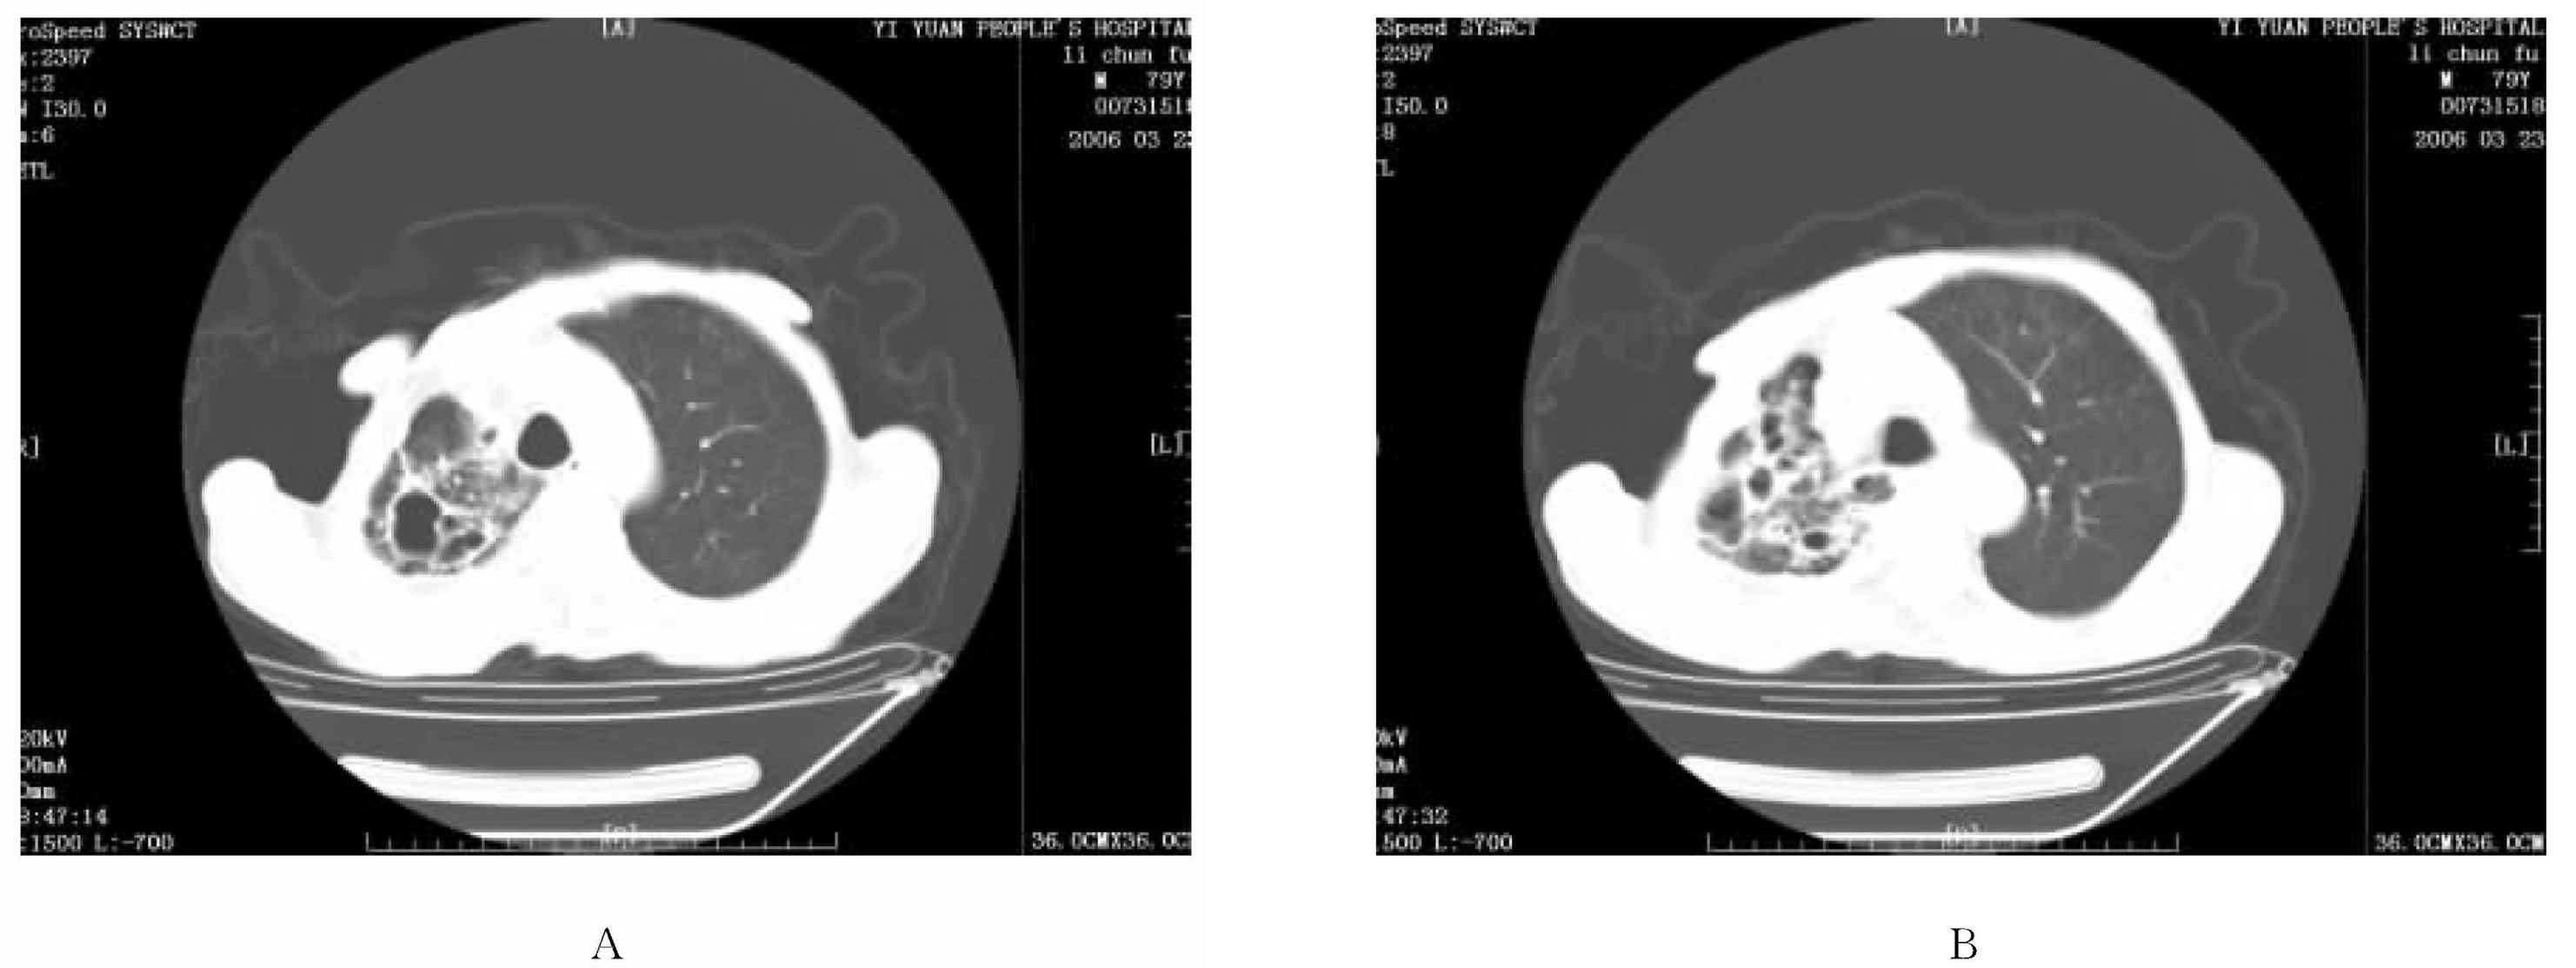
\includegraphics[width=.7\textwidth,height=\textheight,keepaspectratio]{./images/Image00213.jpg}
 \captionsetup{justification=centering}
 \caption{慢性纤维空洞型肺结核\\{\small A、B为同一患者,右肺上叶多发性不规则纤维空洞,其周围有广泛的纤维条索状高密度灶及新老不一的病灶}}
 \label{fig9-25}
  \end{figure} 

\subsection{支气管结核}

有资料统计,在肺结核病人中10%~20%累及气管及支气管。气管及双侧主支气管结核也称为中央气道结核。

\textbf{【病因病理】}
可有以下几种感染途径:①主要是结核杆菌经支气管周围的淋巴道播散;②其次是痰液中结核杆菌的直接侵犯;③也可为结核性淋巴结炎破溃直接侵犯气道。

本病累及的部位主要是气管下段与双侧主支气管,右侧主支气管多于左侧。结核杆菌在支气管黏膜下产生的病理演变也是从渗出性病灶开始,其后即形成结核结节和干酪性改变。多同时伴有肺内活动性或非活动性肺结核。

\textbf{【临床表现】}
除慢性肺结核的一般症状外,本病还有较为特殊的呼吸系统症状,如黏膜溃疡使痰中带血或整口咯血;经常有阵咳、痰量可多;往往有哮鸣音。此外,痰内可经常有大量的结核杆菌。

\textbf{【CT表现】}
气管的狭窄或阻塞。轻或中度向心性管状或漏斗状狭窄,狭窄段较长或主、叶、段多支气管受累是结核性支气管狭窄的常见表现。邻近还可见纵隔或肺门淋巴结增大及其对气管的压迫,以及合并的肺内结核。可继发局限性、阻塞性肺气肿和肺不张,张力空洞等改变,合并其他细菌感染出现相应表现。

1.活动性病变:表现为气管不规则狭窄、管壁明显增厚(可达4~6mm),常伴邻近淋巴结增大与肺内活动性结核。增强扫描可见增厚的管壁有强化。治疗6个月以上气道狭窄与阻塞明显减轻或消失,淋巴结增大减轻,管壁变薄、变光滑,同时肺内病灶有吸收或缩小。

2.非活动性病变:气管狭窄但较光滑,管壁增厚较轻或不明显,可伴有或不伴有肺内活动性结核。

\textbf{【鉴别诊断】}
应与结节病、气管淀粉样变性、恶性肿瘤、非结核性分支杆菌感染以及复发性多软骨炎等鉴别,但主要应与支气管肺癌鉴别。结核性气管病变的特点是病变范围较长(1.0~5.0cm),为环周狭窄,无腔内肿块,同时有肺与肺门纵隔淋巴结结核且病人较年轻等。而支气管肺癌支气管狭窄较局限,管腔狭窄为偏心性的,有腔内肿块,病人年龄较大等。但中央气道结核CT显示管腔狭窄伴邻近淋巴结增大,又合并肺不张与阻塞性肺炎时则颇似支气管肺癌,应需支气管镜及活检鉴别。

\subsection{肺底结核}

肺底结核系指发生于一侧或两侧下叶底段的肺结核。病变与发生于上肺的结核基本相同,但空洞和支气管结核的发生率远较上肺结核高。大多起病急剧,有畏寒、发热、盗汗等中毒症状,同时有咳嗽、咳痰、咯血等症状,易误为急性肺炎。仔细寻找空洞、纤维增殖性病灶及小纤维干酪性病灶有助于本病的影像学诊断。

\subsection{先天性肺结核}

由于先天性肺结核的感染途径特殊,入侵的结核杆菌数量多,迟发型变态反应于新生儿不久就形成,而抗原特异性细胞免疫功能尚未完善,以及新生儿IFN-γ生成不足等因素致使其肺部病变的发生、发展和影像学表现并不完全遵循儿童原发性肺结核的模式。

\textbf{【感染途径】}
①从感染的胎盘经脐静脉;②通过吸入受感染的羊水;③通过吞入受感染的羊水。

\textbf{【诊断标准】}
先天性肺结核的诊断标准仍有争议。目前认为能确诊婴儿结核病,必须加上至少下面1条:①出生后1周内发病;②肝原发综合征或干酪性肝肉芽肿;③胎盘和(或)母体生殖道结核感染;④通过详细的调查排除出生后感染。但排除产前产后感染仍有困难,尤其②、③亦难以证实。发病时间是诊断先天性肺结核的重要依据。后天性结核感染通常需经4~8周产生迟发型变态反应和细胞免疫后才发现较明显的症状和肺部病变。故先天性肺结核多发病于1~2周内,发病越早,可能性越大。如再加上其余3条的任何1条或临床有明显肝大时,则先天性肺结核的诊断基本成立。

\textbf{【临床表现】}
其症状常于出生后1~2周出现。呼吸窘迫、肝脾大和发热是最常见的症状和体征。

\textbf{【影像学表现】}
肺部病变常广泛多发,境界模糊,不易局限,发展迅速,淋巴结增大可有可无,缺少特征性。

国内有学者认为以下两种方式有一定影像学特征:①两肺弥漫性粟粒性病变:主要由血行播散所致,呈边缘模糊的细颗粒状或点片状病灶,且有融合趋势。②两肺广泛分布的斑片-结节状病变:可能为粟粒结核发展而来,或由吸入感染了结核菌的羊水经支气管播散所致。

\subsection{肺结核的合并症}

常见的合并症有:①肺不张;②肺气肿:瘢痕旁肺气肿、局限性肺气肿、肺大泡、肺气囊肿、代偿性肺气肿;③支气管内膜结核;④支气管扩张;⑤并发肺癌。

结核杆菌侵犯支气管,由于持久的支气管结核感染和阻塞而产生的扩张,称为结核性支气管扩张,邻近常伴有活动性肺结核。随着慢性肺结核的纤维收缩,支气管被牵拉而产生扩张(邻近的病灶已愈合或已经长久稳定),可称为继发性支气管扩张,但往往统称为结核性支气管扩张。CT有利于对支气管扩张的显示。

\section{肺真菌病}

\subsection{概述}

\subsubsection{致病真菌的分类}

真菌的生活形态常呈两种类型:一种为菌丝,见于真菌的自然状态;另一种为酵母样,见于人体组织内。

致病的真菌种类很多,一般根据其形态、特性可分为5种:①酵母菌:如新形隐球菌;②酵母样菌:如白色念珠菌;③双相菌类:如组织胞浆菌;④霉菌类:如曲菌和毛霉菌;⑤细菌样菌:如放线菌和奴卡菌。

\subsubsection{肺感染的方式}

肺真菌病的感染方式有两类:①原发性感染:即吸入大量被真菌孢子所污染的物质和尘土所致;②条件性致病或继发感染:患者常有全身性疾病的基础,加之滥用药物(如激素、抗生素、抗肿瘤药物)所致。

\subsubsection{肺真菌病的病理变化}

真菌在肺内的病理变化可有过敏反应、急性炎症、化脓性病变以及慢性肉芽肿,最后纤维化、钙化而愈合。真菌除引起支气管炎、肺实变外,还可侵犯胸膜和胸壁,有的引起肺门淋巴结增大。

\subsubsection{影像学分型}

可分为5型:①肺炎型;②支气管肺炎型;③肺脓肿型;④炎性肿块型;⑤霉菌寄生型(曲菌球)。多先在炎性病变的基础上形成结节,且病灶的多样性是其特点(图\ref{fig9-26})。

在下述情况下应考虑到本病:①肺内病变与临床症状不符,且又无某种疾病的特征;②肺内病变按照炎症或抗痨治疗无效;③类似结核病者,痰检阴性;④出现并发症如胸壁漏管、肋骨破坏和皮肤真菌病等。但本病的诊断无论是临床还是影像学均缺乏特异性。

\begin{figure}[!htbp]
 \centering
 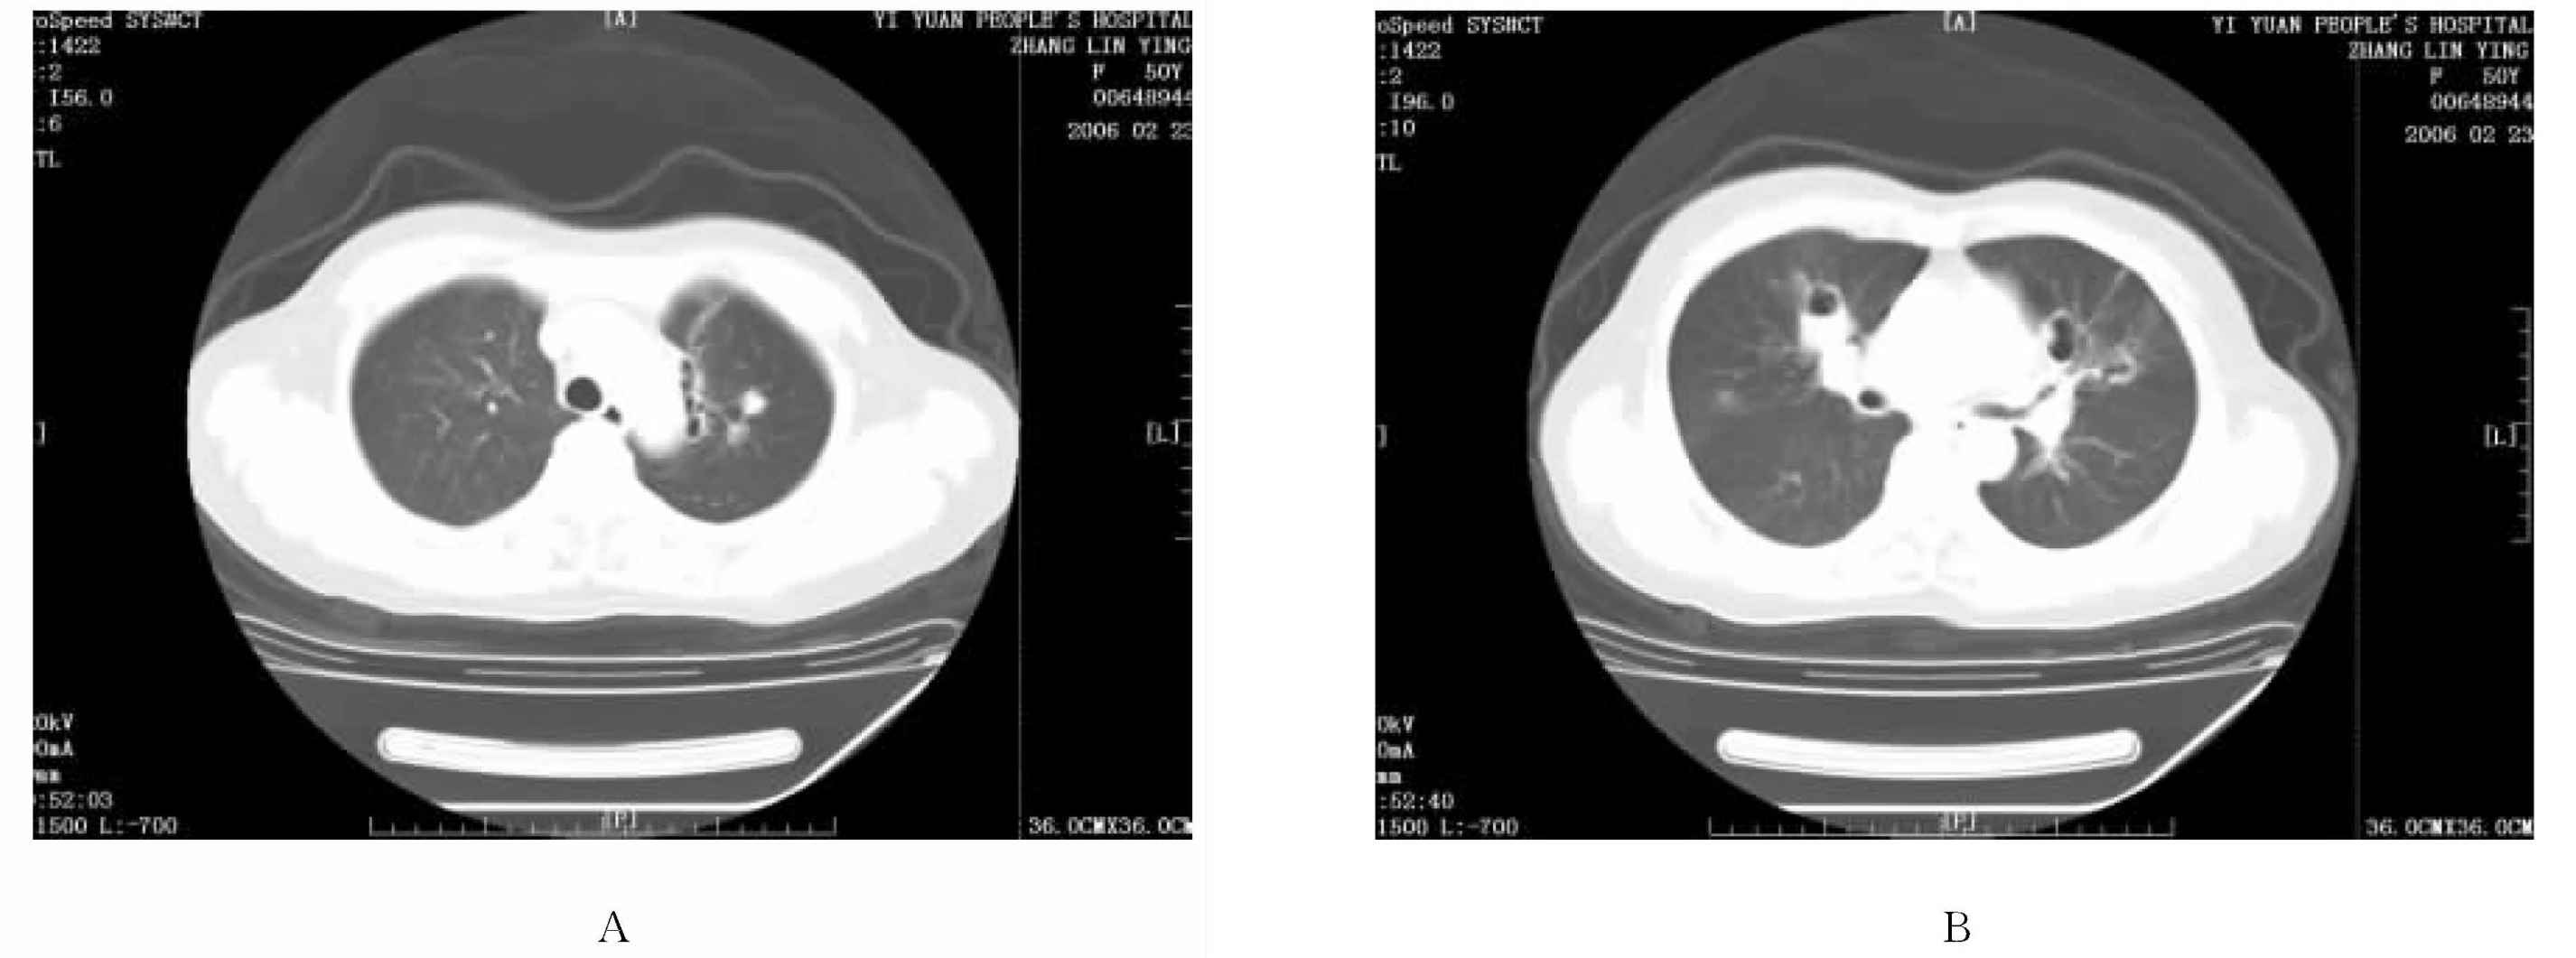
\includegraphics[width=.7\textwidth,height=\textheight,keepaspectratio]{./images/Image00214.jpg}
 \captionsetup{justification=centering}
 \caption{肺真菌病\\{\small A、B为同一患者(经真菌培养和治疗证实),左右肺有许多高密度结节和薄壁空洞,还有斑片状高密度灶}}
 \label{fig9-26}
  \end{figure} 

\subsection{肺隐球菌病}

本病仅次于肺曲菌病,占20%左右,是由新型隐球菌引起的亚急性或慢性深部真菌感染,除常侵犯肺部外,也常侵犯中枢神经系统(易引起脑膜炎)以及其他内脏。此菌为土壤、牛乳、鸽粪和水果的腐生菌。感染途径有内源性、外源性和继发性等。75%以上继发于严重疾病的末期,长期接受激素、抗癌药或广谱抗生素的病人易诱发本病,也可与结核或淋巴瘤并存。

\textbf{【病理】}
主要变化为肉芽肿形成,有巨噬细胞、多核巨细胞、淋巴细胞浸润;病灶中心非化脓性干酪坏死而形成空洞。但化脓、纤维化及钙化少见,不形成明显包膜。病理类型有3种,即孤立性肉芽肿型、粟粒性肉芽肿型、肺炎型。后两型主要见于免疫功能低下或长期应用免疫抑制剂者,可累及多个肺叶;孤立性肉芽肿型则多见于机体免疫力正常者,也可多个肺叶受累。

\textbf{【临床表现】}
多无症状或仅有轻微的一般症状,如咳嗽、咯痰、胸闷、低热、乏力等;少见的症状包括气促、盗汗、食欲不振、恶心呕吐、体重下降;很少出现血痰及急性肺炎表现。侵犯中枢神经系统后可出现脑膜炎和脑膜脑炎的症状和体征。约1/3的患者有影像学的异常而无临床症状。

\textbf{【影像学表现】}
其影像学表现形态各异,具有多态、多样、多病灶和大小不一的特点。

1.常见表现有:①结节或肿块病变:大小0.6~10cm不等;单发或多发(亦有文献报道常为单发);少数病灶边缘可有分叶和毛刺与肺癌难以鉴别;少数有边缘光滑的空洞形成;40%病灶周边或邻近肺野有磨玻璃样模糊影即晕征;多位于肺外带及胸膜下。②浸润实变病变:病灶大小不等,形态各异,可为小条片状、团片状、单叶或多肺叶病变,边缘模糊、密度不均,可见“支气管气像”或“空泡征”,部分可见空洞。③弥漫混合病变:表现为结节、斑片、团块、大叶实变多样化病灶共存。

2.少见表现有:间质肺炎型、弥漫粟粒影、空洞型、合并钙化、胸腔积液、肺门和纵隔淋巴结增大等。

总之,本病不易与肺癌和结核鉴别。国内有学者认为,对位于胸膜下的孤立肺结节或肿块,形态不规则,边缘无毛刺、无分叶或浅分叶,如有厚壁空洞且洞壁光滑,患者临床症状轻微或无症状,在诊断肺癌或肺结核时,应慎重考虑。HRCT有助于鉴别,必要时应活检或抗真菌药物(如Flaconnazal)试验治疗。

\subsection{肺念珠菌病}

念珠菌广泛存在于自然界,其中致病的有白色念珠菌和热带念珠菌,但以白色念珠菌常见。

\textbf{【病理】}
常见的改变为急性炎症和凝固性坏死,常伴多发脓肿。脓肿外围有中性粒细胞和组织细胞浸润。慢性期亦可形成肉芽肿。

\textbf{【临床表现】}
多见于幼儿、老年人及慢性病长期衰弱的病人。一般发病缓慢,病程较长。轻者可无症状,主要表现为咳大量白米浆水样痰或痰血;重者有畏寒、发热、盗汗、气急等症状;血行播散型可有神经系统症状。

\textbf{【影像学表现】}
①支气管炎型:累及支气管壁和周围组织,病程较长时可伴有纤维化及肺气肿。②肺炎型:常表现为支气管肺炎,亦可融合呈节段性;大片实变中可有空洞。③播散型:两肺多发片状、粟粒状高密度灶,中心坏死形成低密度区,亦可形成脓气胸。总之,其血行播散可导致两肺弥漫性微脓肿(呈粟粒性结节)、感染性血栓及出血性肺梗死。CT下出血性结节(见于出血性梗死)可形成“晕”征。

\subsection{肺曲霉菌病}

本病的病原主要为烟曲菌,少见者为黑曲菌和黄曲菌,多发病于慢性病病人免疫功能低下者。本病分为以下3型:

\subsubsection{腐生型}

\textbf{【病理】}
主要改变是曲霉菌寄生于肺内原有的空洞或空腔内,形成曲菌球。曲菌球由菌丝、菌体、黏液和纤维素等构成。

\textbf{【临床表现】}
一般无临床症状。血清凝集试验多呈阳性,而皮肤试验呈阴性。

\textbf{【CT表现】}
特征性表现为空洞或空腔病变内的高密度结节影,其大小约为3~4cm,边缘清楚。如结节完全充满空洞(腔)呈单纯结节状影像。应注意与空洞(腔)性病变内的凝血块、结核干酪空洞及肺癌空洞等鉴别。变化体位观察,球形影像的位置移动有助于本病的诊断。

\subsubsection{}

\textbf{【病理】}
基本病理改变是由于变态反应、支气管分泌黏液增多且合并曲霉菌菌丝,使黏稠度增加,分泌物不易咳出,形成支气管黏液栓塞。

\textbf{【临床表现】}
患者有哮喘病史。实验室检查见嗜酸粒细胞增多、血清IgE蛋白增高、血清凝集试验阳性。

\textbf{【CT表现】}
为支气管黏液栓塞的表现,呈条状、Y型、V型、手指套状或结节状致密影。支气管内黏液栓咳出后呈支扩表现。

\subsubsection{侵袭型}

本型多发生于免疫抑制或免疫力低下的患者,死亡率高达30%~90%。

\textbf{【病理】}
主要改变为支气管肺炎,以及由其破坏肺小血管和支气管而引起的出血性肺梗死。血行播散占20%~25%,其他脏器如肾脏亦可受累。

\textbf{【临床表现】} 患者有高热、咳嗽、呼吸困难、咯血等症状。

\textbf{【CT表现】}
①绕有晕征的结节:即结节周围有低于结节密度、高于肺实质密度的环形带状区,不典型时表现为结节边缘模糊毛糙。其病理基础是出血性肺梗死引起结节中心凝固性坏死,相邻肺泡出血所致。结节加晕征是其较特征性的早期表现,见于40%~69%的早期病例。但该征亦可见于念珠菌病、毛霉菌病、原发性或转移性肿瘤、其他炎症性疾病等。②楔形实变影:表现为以胸膜面为基底的节段性实变影,边缘模糊,与栓塞性肺梗死相似。可单独出现,也可合并结节影和(或)晕征。其病理基础为出血性肺梗死,该征亦可为早期表现,且出现率达80%。但该征还可见于毛霉菌病、细菌性肺炎或肺出血等。③气道播散的表现:表现为小斑片状、片状、磨玻璃状高密度灶,进而可融合成肺段和肺叶的实变,亦可形成空洞,并可伴胸腔积液。④血行播散的表现:呈肺内广泛分布的粟粒结节。

\subsection{肺组织胞浆菌病}

本病由荚膜组织胞浆菌引起,感染力极强,国内少见。

\textbf{【病理】}
主要变化为肉芽肿形成,中心坏死,以后纤维化和钙化。早期与原发性肺结核很相似,组织反应有肉芽肿形成,中心干酪坏死,周围有多核巨细胞、上皮样细胞、淋巴细胞和浆细胞。有自愈倾向,很快纤维化和钙化。少数抵抗力低的病人,可发生全身播散。可侵及肺门纵隔淋巴结,甚至穿破淋巴结形成纵隔炎及纤维化;侵及胸膜则引起胸膜炎和脓胸。

\textbf{【临床表现】}
大多(尤其是原发性感染者)无明显症状,轻者可有低热、咳嗽、咯痰、胸痛、乏力等。重者则有高热、咳嗽、咯痰、贫血、消瘦等症状,有时肝、脾、淋巴结增大。侵犯皮肤或黏膜者可出现结节或溃疡。

\textbf{【影像学表现】}
可分为5型:①结节肿块型:大多单个,也可多个,大小不一,可形成空洞,常伴胸膜增厚。②炎症浸润型:常见于两肺上叶和下叶背段,单发或多发,以后纤维化或钙化。重者可形成空洞,亦可广发浸润类似大叶性肺炎。③粟粒型:由血行播散所致,以后钙化愈合,钙化斑点较粟粒性肺结核的钙化略大而圆。④淋巴结型:肺门及纵隔淋巴结增大,也可形成纵隔炎,甚至可导致上腔静脉阻塞及肺动、静脉阻塞,愈合时表现为淋巴结钙化。⑤混合型。

总之,本病的后期钙化较多而明显,其他则与结核相似。

\subsection{肺放线菌病}

常见的致病菌为以色列放线菌。本病多见于口腔卫生不良者,感染方式为内源性,继发性少见。

\textbf{【病理】}
开始为肺泡炎症,以后成为慢性化脓性肉芽肿,伴结缔组织增生,形成结节和团块,其中混有脓肿。常侵及胸膜和胸壁,引起胸膜炎、脓胸及胸壁瘘管。

\textbf{【临床表现】}
发病时往往症状不明显,不发热或仅有不规则低热、乏力、轻度咳嗽。严重时有寒颤、弛张热、盗汗、咯黏液脓痰等。侵及胸膜、胸壁者可出现胸痛、瘘管。

\textbf{【影像学表现】}
早期为感染性支气管炎表现,以后发展为支气管肺炎或节段性肺炎,进一步形成团块状或不规则阴影。其中有小的低密度空洞,可见引流支气管。胸膜病变表现为胸腔积脓、脓气胸和胸膜增厚。脓胸、肋骨骨髓炎和胸壁瘘管为本病的特点。本病可出现广泛的肺纤维化。

\subsection{奴卡菌病}

本病由星形奴卡菌或巴西奴卡菌所致,遍布世界各地,我国有分散的病例发生。

\textbf{【病理】}
为亚急性、慢性化脓性病变,很少形成肉芽肿。开始为肺泡炎症,有中性粒细胞和淋巴细胞浸润,进而成为肺脓肿。慢性期可伴有纤维化;可侵及胸膜、再至骨骼,免疫力低下者可引起血行播散;易侵犯中枢系统和肾脏,形成多发脓肿。

\textbf{【临床表现】}
初期症状不明显,常有发热、咳嗽、咯痰、乏力等症状。有空洞形成者可咯血。侵及胸膜胸壁者可出现胸痛或瘘管。侵犯中枢系统有相应的症状和体征。

\textbf{【影像学表现】}
与放线菌病相似。①小片状或节段性肺炎,也可为多发散在斑片状高密度灶,亦可有多发结节或空洞;②肺门淋巴结可增大;③侵犯胸膜则可见到胸腔积液、液气胸和胸膜增厚;④肋骨破坏和胸壁瘘管少见。

\subsection{蘑菇肺}

本病是由于大量栽培蘑菇时吸入蘑菇菌类孢子致病。其致病机理目前认为是Ⅲ型和Ⅳ型变态反应介导的肺泡变态反应,其本质是外源性过敏性肺泡炎。

\textbf{【临床表现】}
吸入后5~6小时出现类似流感和细菌感染的临床症状,症状持续24~48小时后消退。可有咳嗽、发热、呼吸困难,肺底捻发音或裂帛音。长期吸入可呈慢性表现,数月内症状消退。

\textbf{【影像学表现】}
①两肺多发大小不等的斑片状模糊阴影,肺尖、肺底分布较少;②弥漫性网织状、结节状影;③肺呈磨玻璃状密度增高;④支气管血管束模糊毛糙;⑤晚期可呈蜂窝状,亦可见肺大泡;⑥有时可见肺门淋巴结增大,酷似结节病;⑦亦可出现心衰表现。

\subsection{青霉菌病}

本病又称帚形菌病,由马尔尼菲青霉菌(Pencillium
Marneffei,P.M)所致,是近些年来新认识的疾病。本病主要发生于东南亚及我国广西与越南交界地区,存活率仅占20%。早期诊断及时应用两性霉素B或制霉菌素、5-氟脲嘧啶、酮康唑可获痊愈。本病通过接触性感染,经呼吸道和消化道吸入,以及皮肤感染引起播散。

\textbf{【病理】}
主要改变为溃疡和肉芽肿病变。可侵及皮肤、淋巴结、胸部及骨骼。淋巴结为反应性增生的肉芽肿和中心坏死的化脓性病变。骨骼为溶骨性病变。关节滑膜有纤维母细胞增生,其中含有上皮细胞的肉芽肿病灶散在少量朗罕氏巨细胞和干酪坏死区。

\textbf{【临床表现】}
分为原发性和继发性。常急性起病,也有呈慢性发病者。常有畏寒和发热、盗汗、贫血、肝脾肿大。胸部还有咳喘、胸痛和咯脓痰,还可见皮肤病损、关节肿痛等。

\textbf{【影像学表现】}
随所累及的部位而异。①胸部:多有肺门淋巴结增大;肺炎呈单发或多发大片或小片状浸润影;肺脓肿呈单发或多发性;还可呈弥漫性粟粒病变;可有胸腔积液和心包炎。②骨关节:表现为边缘清楚的溶骨性破坏伴轻微的骨膜反应性骨硬化。好发于短管骨,其次为长管骨和关节,以及脊柱、肋骨、锁骨、肩胛骨和胸骨。确诊需从病变中分离出P.M。

\section{肺寄生虫病和艾滋病}

\subsection{胸部包虫病}

本病是犬绦虫蚴寄居肺内发育成为包虫囊肿。包虫病最常见的部位是肝,其次是肺,是一种地方病,以牧区多见。

\textbf{【病理】}
其囊壁分为两层,外层为白色半透明的、坚韧的角皮层,内层为胚层或称为生发层。内层分泌澄清的液体,还向囊腔内长出无数的雏囊,内有5~30个头节。雏囊和头节可脱落而悬浮在囊液中,形如细砂。部分生发层可脱离囊壁而形成子囊,子囊一般都在囊内。囊肿外的一层纤维包膜是宿主机体的组织反应,称为外囊。当囊壁破裂,其旁可出现子囊。

\textbf{【临床表现】}
较小者一般无症状。大者多有胸痛、咳嗽、咯痰、胸闷、呼吸困难等症状,其次为咯血、发热。有些同时有荨麻疹、哮喘等过敏反应。Casoni试验或补体结合试验多呈阳性。

\textbf{【CT表现】}

1.肺包虫病的一般表现:病灶以单发多见,呈圆形或椭圆形,边缘清晰而光滑;大者可形态不规则或呈分叶状。大小不一,可为1~10cm,70%的病灶>5cm。其密度均匀,CT值多<20Hu,无强化。外壁较厚,可能是周围肺组织压迫不张所致。少数囊壁可见钙化。囊内囊较少见,但有特征性。子囊密度多低于母囊,多个子囊充满母囊时,呈多房性或蜂窝状。

2.囊肿破裂后表现:①外囊仅有破裂小口,少量空气进入内、外囊之间,呈新月形含气低密度影。②如内、外囊均破裂,空气进入内、外囊,则囊内出现液平面,其上方可有两层弧形含气带,称为“双带征”。③如内囊陷落于液面上呈“水上浮莲征”,为本病的特征性表现。④如液体完全排出呈环状含气影。⑤如液体完全排出,囊肿缩小仅剩内、外囊,其CT值可很高,与肺癌难以鉴别。⑥如破入胸膜腔形成胸腔积液或液气胸。

3.肺包虫囊肿合并感染:①囊内密度增高或密度不均;②囊壁增厚;③囊肿边缘模糊;④可见气泡影及多房影。

4.胸膜包虫囊肿:沿胸壁或纵隔面的半圆形高密度影,边缘清晰,与胸壁或纵隔呈钝角,亦可见内囊破裂。

5.纵隔包虫囊肿:很少见,多见于后纵隔。

6.膈肌包虫囊肿:非常少见,易误为肝包虫病,鉴别常较困难。

\subsection{肺血吸虫病}

血吸虫病的胸部侵犯除尾蚴经过时引起的损害外,主要因虫卵沉积所致。此外,亦有成虫肺内寄生的可能。

\textbf{【病理】}
血吸虫尾蚴经过肺组织主要引起充血、出血和以嗜酸性细胞为主的炎性浸润。虫卵在肺小动脉内分泌毒素,引起急性炎症和组织坏死。大量嗜酸性细胞聚集于虫卵周围形成嗜酸性脓肿。虫卵死后脓肿吸收,其周围产生肉芽组织,中性粒细胞、嗜酸性粒细胞被上皮细胞代替,其中杂有异噬巨细胞,形成假结核结节。虫卵和假结核结节可机化,虫卵亦可钙化。

\textbf{【临床表现】}
急性期病人往往急骤发热,持续时间长。肝、脾增大并有压痛。呼吸系统表现为咳嗽,多为干咳,痰少、呈白色。少数可无呼吸系统症状。周围血象WBC升高,其中以嗜酸粒细胞增加较为显著。发病2周后大便中可找到血吸虫卵。慢性期可有腹泻、下痢等表现。晚期可出现肝硬化、腹水等表现。

\textbf{【影像学表现】}
①弥漫性粟粒状高密度灶:为最常见的表现,一般于感染2个月后出现。它是虫卵引起的嗜酸性脓肿和假结核结节。以中、下肺为多,肺尖少见。大多为1~2mm,少数可达4~5mm,甚至可融合达7~8mm。其大小、形态、密度十分均匀。②片状及絮状高密度灶:少数出现,约1~3cm,呈对称分布,多见于中、下肺。③单发大片或块状高密度灶:极少见。④肺动脉高压:可因长期反复感染使肺动脉分支被血吸虫卵长时间栓塞,引起肺动脉高压,致左右肺动脉、主肺动脉扩张。⑤偶见胸膜轻度受累,而有少许积液或轻度胸膜增厚。

\subsection{肺吸虫病}

本病多由于食入已感染的生虾、蟹、蝲蛄等致病。蚴虫穿过肠壁进入腹腔,再穿过横膈及胸膜进入肺组织,在肺内发育为成虫。

\textbf{【病理】}
肺内的早期改变为虫体刺激引起的局部炎性浸润及出血。虫体在肺内穿行,形成隧道样空洞。后期纤维组织增生包埋虫体形成囊肿,进而硬结、钙化。病理分为出血期、囊肿期和愈合期。

\textbf{【临床表现】}
起病隐匿,可有咳嗽、咳白黏痰、咯血、胸痛、低热、盗汗等症状。咯出果酱色黏痰为本病的特征。在痰中可查到嗜酸粒细胞、夏柯-雷登结晶或肺吸虫卵。

\textbf{【CT表现】}
①浸润性病灶:见于早期,呈片状,主要位于中、下肺。②囊状病灶:代表囊肿期,呈不规则蜂窝状,典型的可见隧道样空腔及不规则线状高密度灶。囊腔大小0.4~2.0cm,囊内含液或气,周围有高密度纤维条索。③结节状高密度灶:代表囊肿的后期,有大量肉芽组织增生,1~2cm大小,其中可有空泡。④硬节或钙化灶:代表愈合期,硬节灶大小不等,多为3~6mm。钙化灶更小,可呈斑片或条状钙化。此外,可有胸膜增厚、气胸,继发感染形成脓胸。

\subsection{肺囊虫病}

囊虫病为猪肉绦虫的囊尾蚴寄生在人体而导致的疾病。其寄生部位很广,常见的顺序为:皮下组织、肌肉、脑、眼、心脏、舌、口、肝脏、肺、腹膜、上唇、乳房、子宫、神经鞘、骨。

\textbf{【病理】}
组织中的囊尾蚴一般被一层纤维囊所包围,其外有细胞浸润,以后发生纤维样变,死后逐渐钙化。

\textbf{【临床表现】}
极为复杂,常见的症状为癫痫。肺部症状症状不著,可有咳嗽等症状。

\textbf{【CT表现】}
肺内病变表现为肺内散在分布的、大小均匀的高密度小结节影,边缘清楚;直径<10mm,以5.0mm左右多见。

\textbf{【鉴别诊断】}
粟粒性肺结核病灶较小,直径约2.0~3.0mm;肺转移瘤大小不均,有助于鉴别。但肺囊虫病需密切结合临床及脑、肝(呈多发囊状低密度)等部位的病灶进行诊断和鉴别。

\subsection{胸部阿米巴病}

阿米巴原虫可在肺部和胸膜上产生以化脓为主的病变。

\textbf{【病理】}
感染途径:①由阿米巴肝脓肿穿破横膈到肺或胸腔;②淋巴传播;③血行播散。病理上肺部阿米巴病变以脓肿形成为主,表现为肺组织的炎变、坏死和化脓。胸膜病变常由阿米巴肝脓肿穿破横膈到胸腔或由肺阿米巴脓肿破入胸腔所致。

\textbf{【临床表现】}
多有发冷、发热、咳嗽、咯痰,痰开始黏稠或带血丝,几天后转变为典型的稠厚棕褐色脓痰。

\textbf{【影像学表现】}

1.由肝脓肿穿破横膈而产生的阿米巴肺脓肿:多见于右肺下叶,其次为中叶。右膈升高变平、活动受限、轮廓模糊。肺内有片状阴影,脓肿多位于下叶前方。常有胸腔积液或脓,心包积液相对罕见。

2.血行播散的肺阿米巴病变:可发生于任何部位,可单发或多发。病灶表现为脓肿或炎性浸润影,与一般肺脓肿和肺炎很难鉴别。

3.支气管肝瘘或胆瘘:常需造影确诊。此外,结合肠道、肝脏的症状和表现有助于诊断和鉴别。

\subsection{蛔虫性肺炎}

蛔虫幼虫在肺内移行时可引起肺部病变。

\textbf{【病理】}
多认为其幼虫在肺内移行时产生过敏反应,释放血管活性酶,增加毛细血管通透性,而形成肺部浸润灶。

\textbf{【临床表现】}
常在感染后10~14天左右发病。多有近期食生蔬菜史。可有干咳、胸痛,严重时有哮喘、呼吸困难、紫绀等症状,有的出现过敏性皮疹。血中嗜酸粒细胞增高。

\textbf{【影像学表现】}
多呈密度均匀的磨玻璃样高密度灶,多发散在分布。严重时病灶可融合。病灶可自行消退。皮质类固醇治疗有效。

\subsection{肺钩虫病}

\textbf{【病理】}
主要是钩虫幼虫钻入皮肤,进入血管,从肺毛细血管穿过肺脏进入支气管时引起出血、炎症及过敏反应而导致支气管痉挛和局灶性肺水肿。

\textbf{【影像学表现】}
呈短暂的肺泡实变,有密度均匀的斑片状高密度灶,边缘模糊,呈非节段性分布。多呈一过性病变,吸收消退快。

\subsection{卡氏肺囊虫肺炎}

卡氏肺囊虫肺炎(PCP)的病原体属于原虫,当人体先天性或获得性免疫功能低下或缺乏时,作为机遇性感染侵入肺部,停留在肺泡腔、肺泡间质旁。以往多见于6周至6个月的婴儿,现多见于艾滋病病人、经抗癌或激素治疗、接受免疫抑制剂的器官移植病人。其中,艾滋病病人合并的肺部感染60%~85%为PCP。

\textbf{【病理】}
患肺大而重,切面可见融合的实变病灶。显微镜下可见间质内有淋巴细胞和浆细胞浸润,肺泡间隔增厚;肺泡腔内见含有很多空泡的嗜伊红物质。在病灶处肺泡腔内可找到卡氏肺囊虫。

\textbf{【临床表现】}
多数急性发病。有发热(多为低热)、干咳、气促或呼吸困难、胸痛等,还有AIDS的症状如乏力、体重减轻、腹泻、皮疹等。很难从咳出的痰中找到病原体。血液化验WBC可正常或稍有上升。

\textbf{【CT表现】}
主要表现为肺部弥漫性、双侧性、边缘模糊的高密度灶,以两下肺分布为主。①早期弥漫性渗出性病灶类似于间质性病变,呈网状、斑点状。②病变发展极快,大约3~4天后病变融合,呈典型的肺泡渗出性病变的特点。过去一直认为是间质性肺炎,但实际上急性PCP主要是肺泡和含气腔隙的渗出、实变伴有少量的浆细胞浸润。③有时可见到囊状透亮的肺气囊肿,上肺多见,可合并自发性气胸。④罕见胸腔积液,少见肺门及纵隔淋巴结增大、肺不张。⑤如出现结节样病变或空洞等不典型CT表现,则提示混合感染存在。

\subsection{艾滋病(AIDS)}

艾滋病是“获得性免疫缺陷综合征”一词英文缩写“AIDS”的译音。它破坏了人体的免疫系统,使机体丧失细胞免疫功能,从而使患者容易感染和促发各种疾病。免疫缺陷表现为白细胞减少和淋巴细胞(主要是T淋巴细胞)减少。常由性交(同性或异性)、输血或血制品及滥用静脉注射药物等方式传播。患者可出现全身性广泛感染。

\textbf{【临床表现】}
多为非特异性的。一般表现有反复发热、全身不适、体重减轻、盗汗、贫血和全身淋巴结肿大等。呼吸系统主要有病程较长的干咳和呼吸困难,也可以出现急性暴发性呼吸衰竭。

\textbf{【胸部病变】} AIDS的胸部病变多数由机遇性感染所致。

1.卡氏肺囊虫肺炎(PCP):发病率约60%~85%。

2.肺结核:发病率约3.6%~3.8%。

3.不典型分支杆菌感染:①鸟型分支杆菌:最常见,呈斑片状浸润或结节影,易形成空洞;常有淋巴结增大并呈环形强化,胸水也常见;但很少有粟粒状改变。②堪萨斯杆菌:较少见,常表现为肺内孤立结节。

4.真菌感染:发病率近5%。隐球菌病最常见,其次为组织胞浆菌病较多见,曲霉菌、念珠菌、星形奴卡菌以及球孢子菌感染等亦可见到。

5.病毒感染:主要由巨细胞病毒(CMV)、单纯胞疹病毒(HSV)和水痘带状疱疹病毒(VZV)引起。①CMV肺炎:病理上表现为弥漫性肺泡损害、肺间质水肿及闭塞性细支气管炎。影像学最常见的表现为双侧间质性病变如网状或磨玻璃状,也有中、下野散在分布的粟粒、结节和肺泡实变等。常难与PCP鉴别。②HSV肺炎:常同时有皮肤、口腔和食管受累。影像学可表现为双侧间质性病变,但以弥漫散在的肺泡实变多见,其病理基础为坏死、出血和水肿。③VZV肺炎:影像学通常表现为双侧散在的肺泡渗出和结节状影,有融合倾向。

HSV和VZV肺炎亦可影像学表现为正常。肺部病毒感染所致的胸腔积液和胸部淋巴结增大很少见。

6.细菌感染:发病率约3%。常见的致病菌有链球菌、流感嗜血杆菌和假单胞菌属。

7.肿瘤:约1/3出现恶性肿瘤。常见的有:①Kaposi肉瘤:约有25%的Kaposi肉瘤有肺部受累(见本章第十五节)。②恶性淋巴瘤:生长快,倍增时间可短至4~6周。

8.淋巴性间质性肺炎:典型表现为磨玻璃状改变和弥散分布的微小结节。常与PCP相似,但很少进展为肺泡实变。

9.肺大泡。

10.心包、心脏病变:心包积液常由结核引起;偶见心包或心外膜的Kaposi肉瘤。心脏病变为心肌病改变。

\section{肺肿瘤}

肺部肿瘤包括原发性肿瘤和转移瘤,原发性恶性肿瘤以支气管肺癌常见,少数为肉瘤。支气管腺瘤一般认为是低度恶性肿瘤,组织学分为类癌、黏液表皮样癌和腺样囊性癌。

肺良性肿瘤占肺肿瘤的10%,根据来源大致分为3类:①来源于胚胎发育障碍:如错构瘤、畸胎瘤;②来源于间叶组织:如平滑肌瘤、神经鞘瘤、脂肪瘤、血管性瘤等;③来源于支气管壁的上皮或腺体:如支气管乳头状瘤等。

\subsection{肺错构瘤}

本病是肺内最常见的良性肿瘤,严格说不是真性肿瘤,是内胚层与中胚层发育异常而形成的肿瘤样变。发生于肺段及段以上支气管的错构瘤为中央型;发生于肺段以下支气管及肺内的称为周围型。以周围型多见,仅10%位于支气管腔内。

\textbf{【病理】}
在组织结构上一般以软骨为主,其次为纤维组织、平滑肌、脂肪组织、上皮组织、骨组织等。故根据其成分主次可分为软骨型、纤维型、平滑肌型、腺样型等。

\textbf{【临床表现】}
多见于40岁以上男性,男女之比为(2~3)∶1,一般无临床症状,偶尔(尤其中央型)可有咳嗽、咳痰甚至痰血等症状。

\textbf{【CT表现】}
周围型通常表现为圆形或椭圆形孤立性肿块,直径多<5cm。轮廓光滑,无毛刺征象,亦可有浅分叶或边缘毛糙。以软骨成分为主者可有较广泛的钙化,以纤维组织为主者密度均匀。25%~30%可有钙化,典型者呈爆米花状,也可呈斑点状(图\ref{fig9-27})。50%薄层扫描可见脂肪组织,CT值<-40Hu。极少出现空洞。肿瘤生长缓慢,少数亦可增长很快,甚至恶变。增强扫描绝大多数无明显强化。大支气管内者可见边缘光滑的腔内结节并可见阻塞性肺炎、不张等表现;肺段支气管内者仅显示支气管截断和阻塞性改变。

\begin{figure}[!htbp]
 \centering
 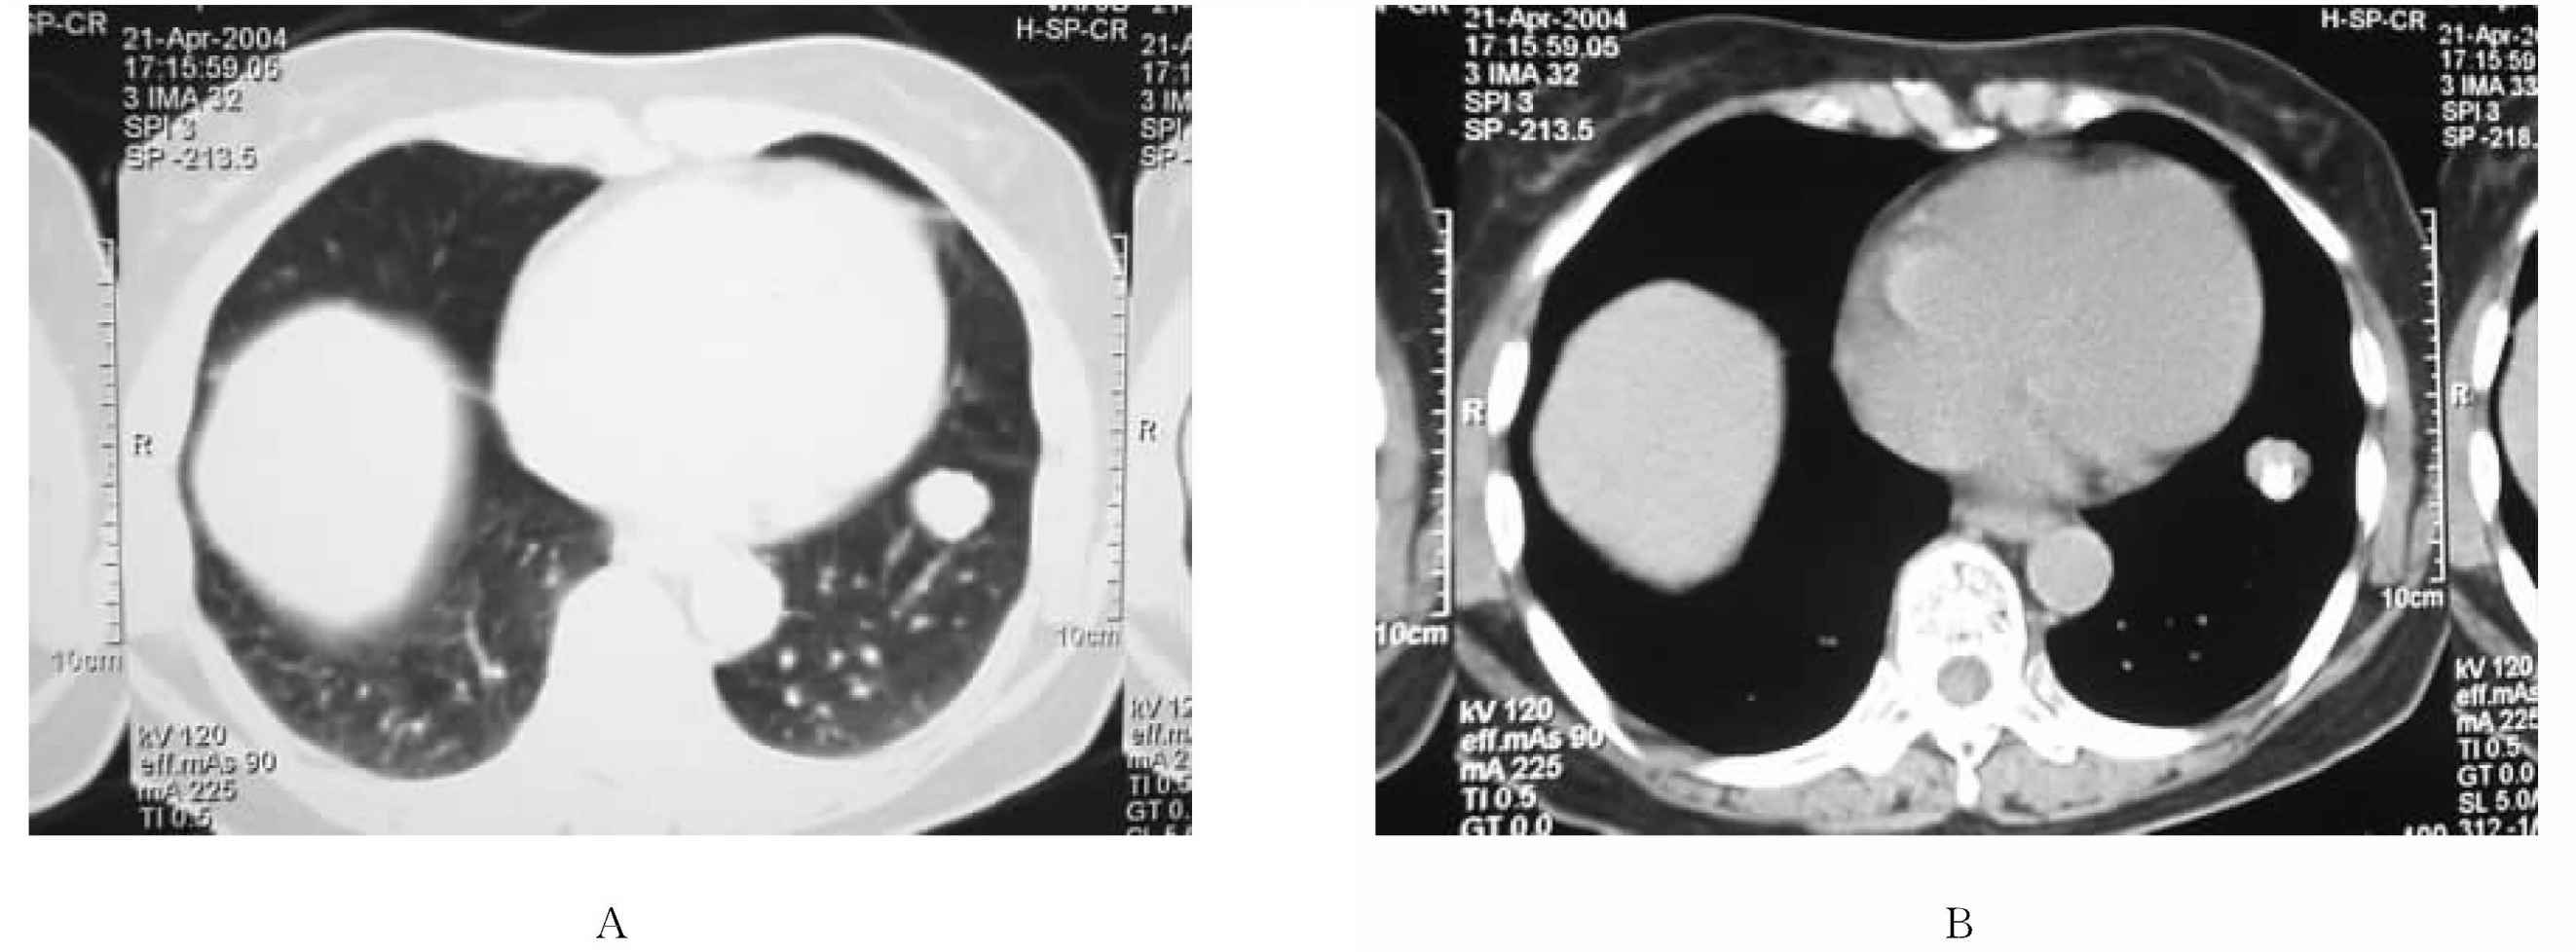
\includegraphics[width=.7\textwidth,height=\textheight,keepaspectratio]{./images/Image00215.jpg}
 \captionsetup{justification=centering}
 \caption{肺错构瘤\\{\small 左下叶内前段有高密度结节,其内有近爆米花样钙化}}
 \label{fig9-27}
  \end{figure} 

\textbf{【鉴别诊断】}
①其他肿瘤:错构瘤既可表现密度均匀,亦可含有脂肪或(和)钙化,利用合理的窗技术,观察肿块内有无脂肪和钙化,结合其边缘光滑等表现是正确诊断的关键。否则,尤其无钙化及脂肪者易误为肺癌,也不易与其他良、恶性肿瘤相鉴别。②畸胎瘤:虽亦有钙化和脂肪,但体积较大(多为5~10cm),常因继发感染而边缘模糊、毛糙,甚至呈大片状有助于鉴别。

\subsection{肺硬化性血管瘤}

本病是一种少见病,应归为良性病变。WHO及国外学者命名为肺硬化性血管瘤,国内则称为假乳头状瘤型或硬化性血管瘤型炎性假瘤。

\textbf{【病理】}
本病的组织来源意见不一,主要有:①血管内皮细胞学说;②间叶起源学说;③神经内分泌起源学说:如国内李维华等曾命名为肺良性神经内分泌瘤;④肺泡上皮细胞起源学说:近些年来的国内外研究认为本病是来源于肺泡上皮的良性肿瘤,应称之为良性肺泡上皮细胞瘤。

病理表现为肿瘤界限清晰、无包膜,呈圆形或卵圆形。组织学主要有表面细胞和圆形细胞2种细胞构成。其组织学亚型有4种:出血型、乳头型、硬化型和实体型。国内还有学者认为本病具有血管瘤样区→乳头区→实性区→硬化区的演变过程。

\textbf{【临床表现】}
本病好发于40~60岁的中年女性,多无自觉症状,可有咳嗽、咯血,甚至有发热、胸痛等症状。

\textbf{【CT表现】}
圆形、椭圆形孤立性肿块,边缘光滑,密度均匀、与肌肉密度相仿,有时有小低密度区和粗大点状钙化,偶见囊性变,无分叶、毛刺和卫星灶。病灶大小多在3.0cm以内。增强扫描早期呈中度至明显强化(国内分别有报道其增强值为70~130Hu和43.23±8.65Hu),强化持续时间长(6分钟病灶强化仍较明显)。肿块<3cm者多呈均匀强化,直径>3cm者呈不均匀强化。不均匀强化是由于血管数目相对较少的实体型和硬化型结构增多且分布不均所致。少数早期呈明显不均匀强化,延时5~10min后病灶密度逐渐变均匀。可伴胸内淋巴结增大。

以上为硬化性血管瘤之特点,但与其他良性肿瘤,以及炎性假瘤不易区别。

\subsection{肺其他良性肿瘤}

肺其他良性肿瘤少见,其种类甚多,如平滑肌瘤、纤维瘤、脂肪瘤、血管瘤、神经源性肿瘤、软骨瘤、黏液瘤、乳头状瘤等。可发生于肺段或肺段以上支气管腔内,也可为肺内肿块。各种良性肿瘤均生长缓慢,有完整包膜。

\textbf{【临床表现】}
常无明显症状,发生于大支气管内者产生阻塞性肺炎,引起发热、咳痰等症状。较大的肺内肿块可有压迫症状。

\textbf{【CT表现】}
①支气管腔内者表现为腔内结节、梗阻(阻塞性肺气肿、肺炎或肺不张等),与恶性肿瘤鉴别困难。②肺内者呈圆形、椭圆形或分叶状软组织肿块,大小不一,边缘光滑清楚。③脂肪瘤CT值<-40Hu。④平滑肌瘤、纤维瘤、血管瘤、软骨瘤均可见斑片状、砂粒状钙化。⑤平滑肌瘤血供较丰富可有明显强化;纤维瘤可有轻度强化;血管瘤可有轻中度强化。

\subsection{支气管腺瘤}

支气管腺瘤这一命名不确切,本病应属恶性。肿瘤起源于气管、支气管的黏液导管的上皮细胞。

\textbf{【病理学分类】}
①从组织学上分为:类癌、黏液表皮样癌和腺样囊性癌,其中90%左右为类癌。②从大体形态上分为:中央型和周围型。

\textbf{【临床表现】}
主要表现为咳嗽、咯血、胸痛,多见于中央型。周围型一般无症状,病程较长。

\textbf{【CT表现】}
①中心型:呈气管、支气管腔内边缘光滑的软组织结节、狭窄或中断。阻塞后可出现阻塞性肺气肿、肺炎、肺不张。有的可见管壁增厚和腔外肿块,亦可见阻塞性支扩及黏液栓。②周围型:呈球形结节或肿块,直径以2.5~5cm多见,边缘光滑、清楚、密度均匀,无分叶或仅有浅分叶。但少数可显示典型的分叶、毛刺及轮廓模糊,而与肺癌难以鉴别。

\subsection{肺神经内分泌癌}

因为类癌与小细胞未分化癌同起源于(但分化程度不同)支气管树黏膜上皮及黏膜下腺体中的神经内分泌细胞(Kulchitsky
cell,KC),故统称为肺神经内分泌癌。

\textbf{【病理组织学分类】}
国外有学者于1985年将肺神经内分泌癌分为3个亚型。①KCC-Ⅰ型:即典型类癌。具有相对良性的生物学行为,病程发展缓慢,预后较好,术后5年生存率可高达100%。②KCC-Ⅱ型:即非典型类癌,又称为恶性类癌,占类癌的11%~24%。具有侵袭性的生物学行为,淋巴转移多见,术后5年生存率为69%。③KCC-Ⅲ型:小细胞内分泌癌。

但上述分类仍难以将某些肺内神经内分泌癌进行归类。因此,1993年有学者建议对神经内分泌肿瘤采用以下方法分类。①良性神经内分泌瘤;②神经内分泌癌:包括典型类癌、不典型类癌、小细胞神经内分泌癌、大细胞神经内分泌癌、巨细胞神经内分泌癌、不能分类的神经内分泌癌。

\subsection{支气管类癌}

本病又称肺类癌,占原发肺癌的1%~2%。上已述及病理组织学分为典型类癌和非典型类癌。

\textbf{【临床表现】}
国内有报道支气管类癌多见于成年男性。国外有报道典型类癌多见于50岁左右的不吸烟女性;不典型类癌多见于60岁左右的吸烟男性。典型类癌和不典型类癌是儿童最常见的恶性肿瘤。周围型一般无症状;在大支气管内生长时,可出现干咳、咯血、呼吸困难、阻塞性肺炎等症状和体征。偶有内分泌症状如Cushing综合征、类癌综合征和巨人症等。

\textbf{【CT表现】}
中心型多见,约占85%,其中3/4起源于叶支气管;周围型占15%。

1.中心型:①腔内生长的、边缘光滑的、清晰的结节,可同时向腔外浸润,直径多在1~2cm。②15%~30%的典型类癌可有局限性或弥漫性钙化。③增强扫描明显强化。④可伴有阻塞性肺炎及不张。⑤典型类癌纵隔及肺门淋巴结增大很少见,而不典型类癌则常见。

2.周围型:①位于肺的周边部,呈单发或多发的圆形、椭圆形结节,边缘光滑,无或有分叶,有时有细毛刺。②病灶较大,2~18cm大小。病灶密度多均匀,有时可见坏死空洞。③约30%可见弥漫性或点状钙化。④增强扫描多呈均匀性显著强化。⑤肺门或纵隔淋巴结增大发生率与中央型相近。

3.典型类癌与不典型类癌的区别:①后者恶性程度高于前者。②后者多为中心型生长,偶见外周型。但国内也有学者认为后者多为周围型生长。③后者肿瘤较大,多为3~4cm左右,边缘清楚,轮廓可不规则。④后者钙化率不及前者,但常见低密度坏死表现。⑤后者淋巴结转移较常见。

4.晚期支气管类癌可出现肝脏、肾上腺、骨骼及脑转移,骨转移多为成骨性。

\subsection{气管支气管腺样囊性癌和黏液表皮样癌}

1998年WHO的肺及胸膜肿瘤病理分类中,将腺样囊性癌(ACC)、黏液表皮样癌(MEC)及腺泡细胞癌等统称为唾液腺型癌。主要发生于气管、支气管的黏膜下浆液及黏液腺。

\textbf{【病理】}
气管支气管涎腺样肿瘤以ACC最常见,其次是MEC。ACC是一种以局部浸润生长为特点的肿瘤。癌细胞小,呈实性条索、腺管或筛状结构,故又称圆柱瘤、筛样癌。发生于气道时可形成一光滑的息肉样肿物,也可沿管壁环形生长。肿瘤在黏膜下浸润,有时可达肿瘤主体相当远的距离。MEC最可能发生于气道黏液腺的外分泌导管,镜下由含黏液细胞及表皮样细胞两种成分组成,且可分为低度恶性和高度恶性。

\textbf{【临床表现】}
ACC和MEC症状相仿。好发于青年人,也可见于儿童和老年人,男略多于女。主要表现为气道阻塞症状,如反复肺部感染、咳嗽、咳痰、喘鸣、呼吸困难和胸痛等。

\textbf{【CT表现】}

1.ACC和MEC的影像学表现:①腔内型肿物:边缘清楚光滑的息肉状,基底较宽有别于良性肿瘤。②腔内外型肿物。③周围型肿物:几乎原发于段支气管,故多邻近肺门,边缘光滑锐利,可有浅分叶及阻塞性改变。④阻塞性病变:包括肺气肿、肺不张、炎症及黏液栓。因生长缓慢,肺气肿形成的机会较多且持续时间长,有时于多年后演变为肺不张。此外,肺门纵隔淋巴结肿大相对少见。

2.ACC和MEC的区别:国内有文献报道区别如下:①位置:ACC最常见于气管;MEC多见于叶及段支气管,主要为叶支气管。②生长方式:ACC腔内外型相对较多,甚至主要位于腔外,界限不清,呈浸润性生长,并常侵及邻近组织、器官;MEC多局限于腔内,边缘清楚,无外侵。③管壁增厚:ACC可见管壁全周或近全周增厚及管腔狭窄,甚至长段狭窄,管壁增厚可与肿物同时存在;MEC基本不出现管壁浸润状增厚。④密度:ACC病灶密度较低,平扫低于或近、等于肌肉,强化不明显(一般均低于肌肉);MEC病灶常明显强化(密度高于肌肉),且易钙化(钙化率达50%)。⑤MEC远端可有支气管扩张及黏液栓形成。

此外,应注意结合临床与类癌及其他肿瘤相鉴别。

\subsection{肺非典型腺瘤样增生}

肺非典型腺瘤样增生(AAH)被认为是腺癌的癌前病变,组织学上类似于非黏液型细支气管肺泡癌。它与高分化腺癌无论从病理学还是影像学均难以鉴别。

\textbf{【病理】}
肺AAH为肺外周局灶的不典型立方或柱状上皮增生,胞浆少、核异型性活跃,取代了正常的肺泡或细支气管-肺泡上皮,沿肺泡间隔匍匐生长,使其轻度增厚,无局灶性纤维变。

\textbf{【临床表现】}
本病女性多于男性,发病年龄55岁左右。多无临床症状,与吸烟无关,胸片常为阴性。

\textbf{【CT表现】}
以HRCT检查为优,呈局限性1~2cm、边缘较清楚、密度均匀的磨玻璃状密度灶。长期随访病变无吸收消失、无条索状纤维化瘢痕,如有血管增生为恶性。

\textbf{【鉴别诊断】}
炎症和结核随访有吸收或纤维化改变是鉴别诊断的关键,随访数月稳定的局限性磨玻璃状密度灶很可能是早期肺腺癌或AAH。此外,还应注意与下列病灶鉴别。①纤维化病灶:不成形、条索状,有牵拉收缩表现,不具备毛刺和分叶等边缘征象;②肺短暂性感染:与AAH或早期高分化腺癌无法鉴别,靠治疗复查;③机化性肺炎:局灶性机化性肺炎(病理上相当于肺间质纤维化和慢性炎性细胞渗出区域,并混杂有肺泡内的水螅样肉芽组织)在HRCT上可表现为明显持久的局限性磨玻璃样密度灶,这些病灶可能被误为细支气管肺泡癌;④炎性肉芽肿;⑤肺间质淋巴结肿大;⑥肺小叶、肺亚段不张:呈絮状、肺纹理聚拢;⑦血管伪影(与血管平行处、分叉处);⑧肺癌:AAH与肺癌鉴别困难。AAH常常呈现为纯磨玻璃状密度灶,而细支气管肺泡癌或腺癌在纯磨玻璃状密度灶和混合性磨玻璃状密度灶的出现率相近。因此根据局限性膜玻璃样密度灶内实性成分的多少在一定程度上可以鉴别肺腺癌和AHH。

\subsection{肺癌}

支气管肺癌绝大多数起源于支气管黏膜上皮,包括细支气管或肺泡上皮,少数起源于大支气管的腺体上皮。

\textbf{【病理】}

\subsubsection{分型}

1.组织学分型:①来自支气管表面上皮的癌:包括鳞状上皮癌(约占35%)、腺癌(约占20%~30%)、腺鳞癌、大细胞癌(约占14%)。但目前认为,以腺癌多见。②来自神经内分泌细胞的癌:包括低分化的小细胞癌(约占24%)、中分化的不典型类癌、高分化的类癌。③来自细支气管Clara细胞和Ⅱ型肺泡细胞的癌:细支气管肺泡癌(约占2%~5%),关于细支气管肺泡癌的组织来源有分歧,也有人认为是腺癌的一种特殊类型,其特点为沿肺泡孔作气道转移。

此外,还有上述的主要发生于气管、支气管黏膜下浆液及黏液腺的唾液腺型癌。

2.根据病理大体形态分型:①管内型;②管壁型:包括管壁型、管内外混合型、管壁外浸润型;③球形;④巨块型:直径>5cm;⑤弥漫型。

3.根据起源部位分型:①中心型:起源于主支气管、叶支气管或段以下支气管已累及叶支气管。②周围型:原发于肺段或更小细支气管。曾有人将仅累及肺段支气管者称为中间型或肺段型。现也有人主张将起源于段支气管以上的肺癌称为中心型,而将起源于更小的支气管的肺癌称为周围型。此外,发生于肺尖内后部的周围型肺癌称为肺上沟癌(Pancoast癌),常为鳞癌。

\subsubsection{生长方式}

1.中心型肺癌:其病理类型以鳞癌多见,其次为小细胞未分化癌,亦可见于腺癌和大细胞癌。

(1)早期生长方式可分为3类。①结节型:以腔内生长为主,较早引起阻塞性改变。②浸润型:主要沿支气管黏膜依长轴方向浸润生长,致管腔狭窄和管壁增厚。③结节浸润型:向管内外双向生长。

此外,浸润型、结节浸润型可沿黏膜下淋巴管浸润,形成远离原发灶的单个或多个黏膜肿块,即所谓“跳跃式”生长。

(2)肿瘤进一步生长可沿着支气管壁向中央侧或末梢侧蔓延。亦可穿过管壁向外发展形成肺门肿块,并致阻塞性改变;且与转移增大的淋巴结融为一体,以致难以判断肿瘤的原发部位。

2.周围型肺癌:以腺癌多见,其他各种病理类型均可见及。发生于段支气管者,由于其管腔较小,早期可致管腔狭窄发生肺段炎症和不张。发生于肺段支气管以远的肺癌主要形成局部结节或肿块。易在肺实质内形成结节或肿块的原因是发生肿瘤的小支气管为菲薄的膜状结构,不能限制肿瘤的生长。这种类型的肺癌其生长方式有以下两种。

(1)浸润性生长(伏壁式生长):瘤细胞不断的经肺泡孔从一个肺泡侵入另一个肺泡,同时可经淋巴、小气道或以直接浸润的方式从一个肺小叶扩展到另一个肺小叶。瘤细胞以肺泡壁为支架,呈单层或2~3层覆盖于肺泡壁并沿肺泡壁连续性生长。此时,因小叶间隔产生增殖性反应,增厚的小叶间隔从一定程度上限制了癌细胞的进一步浸润,因此肿瘤结节不同程度的带有小叶的特点。在其生长过程中,周围阻力不一致,故各个部位生长速度不一,使肿瘤呈分叶状。在瘤体周围,由局部淋巴等蔓延的子灶不断生长与瘤体融合,也使瘤体呈分叶状。

当弥漫浸润性生长时,癌细胞沿肺泡壁呈覆壁生长,逐渐置换肺泡上皮,而肺泡腔仍保持部分充气,肺泡间隔等支架组织不受破坏。受癌组织侵及的肺泡与正常肺泡混杂排列,无显著纤维结缔组织增生。在影像上呈浅淡片状阴影、大叶性实变伴有支气管气相,难以与肺炎鉴别。有时沿气道播散形成两肺弥漫分布的界限不清的腺泡样结节。

(2)膨胀性生长(堆积式生长):瘤细胞增殖成团的充满肺泡腔,并沿肺泡孔向周围呈铸型性生长、膨胀性扩大,形成实体性肿块,压迫周围肺组织产生假包膜,故瘤体界限较清楚。由于其生长不均可有分叶、切迹、脐凹征,亦可坏死形成空洞。瘤体远侧亦可有阻塞性肺炎或不张,以及肺梗死等改变。

\subsubsection{转移方式}

其转移方式有4种。①淋巴转移:是肺癌最常见的转移方式,癌细胞先转移到肺门淋巴结,进一步转移到纵隔淋巴结,进而到胸导管或右淋巴管。当肺门淋巴结转移伴淋巴回流受阻时,发生淋巴逆流,肺浅组淋巴丛受累时出现胸膜淋巴渗透。右下肺的淋巴回流可经食管裂孔或经肺韧带引流到横膈和腹腔淋巴结。以未分化癌的淋巴转移早,发展最快,且原发灶可很小;腺癌淋巴转移亦较早,但淋巴结较小。②血行转移:癌组织侵犯肺静脉,或经纵隔的淋巴结引流入血循环所致。常转移到脑、肝、肾上腺、骨、肾、胰腺等脏器,亦可形成肺内血行转移。以未分化癌和腺癌多见。③直接侵犯:直接侵犯邻近的组织和器官是肺癌的恶性征象之一。④支气管播散:主要见于细支气管肺泡癌和部分腺癌,播散至邻近肺段、肺叶甚至对侧肺。

\textbf{【临床表现】}

1.局部症状:①咳嗽:为最常见的早期症状,约占75%。典型者为阵发性刺激性咳嗽。②血痰或咯血:为第二常见症状,约占50%。一般为痰中带血丝,反复发生。③胸痛:肿瘤位于胸膜下时钝痛和隐痛颇常见,直接侵及胸膜时出现严重的持续性剧痛。④胸闷、气急、喘鸣。⑤渗出性胸水不说明一定有胸膜转移,血性胸水通常为癌组织侵犯胸膜所致。

2.全身症状:①发热:可因阻塞性肺炎、肿瘤坏死、肿瘤本身所致;②消瘦、乏力、纳差、贫血等恶液质表现。

3.肺外表现:因肺癌异位内分泌的作用产生的肺外症状称为副癌综合征。①骨关节肥大(以膝、腕、踝多见)和杵状指、趾;②鳞癌可引起甲旁亢、消化道和精神症状;③腺癌可引起哮喘、皮肤黑色棘皮病和皮肌炎;④小细胞癌可引起类癌综合征、肾上腺皮质功能亢进、低钠血症(抗利尿激素分泌增多所致);⑤大细胞癌可引起男性乳房肥大。

4.肺癌外侵及转移的表现:①胸膜侵犯和转移表现为胸痛、伴或不伴胸水;②心包受侵或转移产生心包积液而出现气急;③喉返神经受侵有声音嘶哑;④上腔静脉受侵产生上腔静脉阻塞综合征;⑤颈交感神经受侵则产生霍纳(Horner)综合征,表现为眼睑下垂、眼球凹陷、瞳孔缩小、患侧无汗和感觉异常;⑥臂丛神经受侵可引起上肢麻木、疼痛、肌肉萎缩;⑦纵隔淋巴结增大压迫食管引起吞咽困难;⑧膈神经受侵产生膈麻痹和气急;⑨脑、肾上腺、肝、骨等转移产生相应的症状。

\textbf{【CT表现】}

\subsubsection{中心型肺癌}

1.平扫表现:其CT平扫表现包括直接征象和间接征象两方面。直接征象主要为支气管改变和肺门肿块;间接征象主要为支气管阻塞的征象。其他表现有肺门纵隔淋巴结增大、胸水、肺内转移等。

(1)支气管改变:①支气管壁增厚:正常管壁厚度均匀且段以上支气管厚约1~3mm。②支气管腔狭窄:1)可表现为向管腔内突入的软组织影(图\ref{fig9-28}A);2)管壁浸润性增厚,局部管壁不规则,其狭窄可表现为局限环形狭窄,也可为管状狭窄;3)支气管腔可由轻度狭窄到完全闭塞呈向心性锥状或鼠尾状、管腔突然截断或管腔呈偏心性狭窄。狭窄的支气管壁可光滑,亦可凹凸不平。

(2)肺门肿块:是其进展期的主要表现,晚期可由原发灶和淋巴结融合而成。边缘不规则,也可有分叶表现。其内可有钙化多为原有的肺门淋巴结钙化。因为常伴有相应的阻塞性改变,掩盖肿瘤的边缘,故毛刺征象不多见。但合并阻塞性癌性淋巴管炎时,其周围可见沿支气管、血管向肺野走行的放射状分布的细条影。单纯的肺门淋巴结增大边缘较光滑,邻近支气管本身常无异常或仅受压移位,有助于与中心型肺癌的肿块鉴别,但有时鉴别困难。

(3)支气管阻塞表现:如侧支通气发达,个别病例即使阻塞很明显也无阻塞征象。①阻塞性肺气肿:为局限性,是最早的改变(图\ref{fig9-28}B)。应注意与进展期肺癌邻近肺叶或肺段的代偿性肺气肿相鉴别。②阻塞性肺炎:因分泌物引流不畅而致感染,常伴部分性肺不张,可表现为小叶或小叶融合、肺段和肺叶实变。其特点为肺门部有肿块、缺乏空气支气管征,且炎症抗炎治疗不易吸收或反复发生。脓肿形成是其另一常见并发症。③阻塞性肺不张:肺门部肿块可突出于不张的外缘(图\ref{fig9-28}C)。④阻塞性支扩和黏液栓塞:以增强扫描时显示为优,呈低密度条状,形态多样。

(4)肺血管改变:癌组织直接侵犯、癌块或(和)增大淋巴结直接压迫邻近血管,导致血管结构变形、狭窄、形态不规则甚至中断。肺不张时血管聚拢,局限性肺气肿时该区域肺血管稀少。

(5)胸腔积液:多意味着胸膜转移和侵犯。常伴有阻塞性肺不张,而纵隔移位不著。当胸膜不规则增厚、有壁结节时更支持胸膜受累。但亦有部分胸水是淋巴回流受阻所致。

(6)肺门、纵隔淋巴结转移:有时虽有淋巴结转移,但并非一定增大;同样,淋巴结增大并非代表淋巴结转移。国外有学者提出正常淋巴结的边缘是凹或直的,如肿胀或改变形状就会突向肺实质面,故应结合其形态予以诊断(图\ref{fig9-28}D)。

\begin{figure}[!htbp]
 \centering
 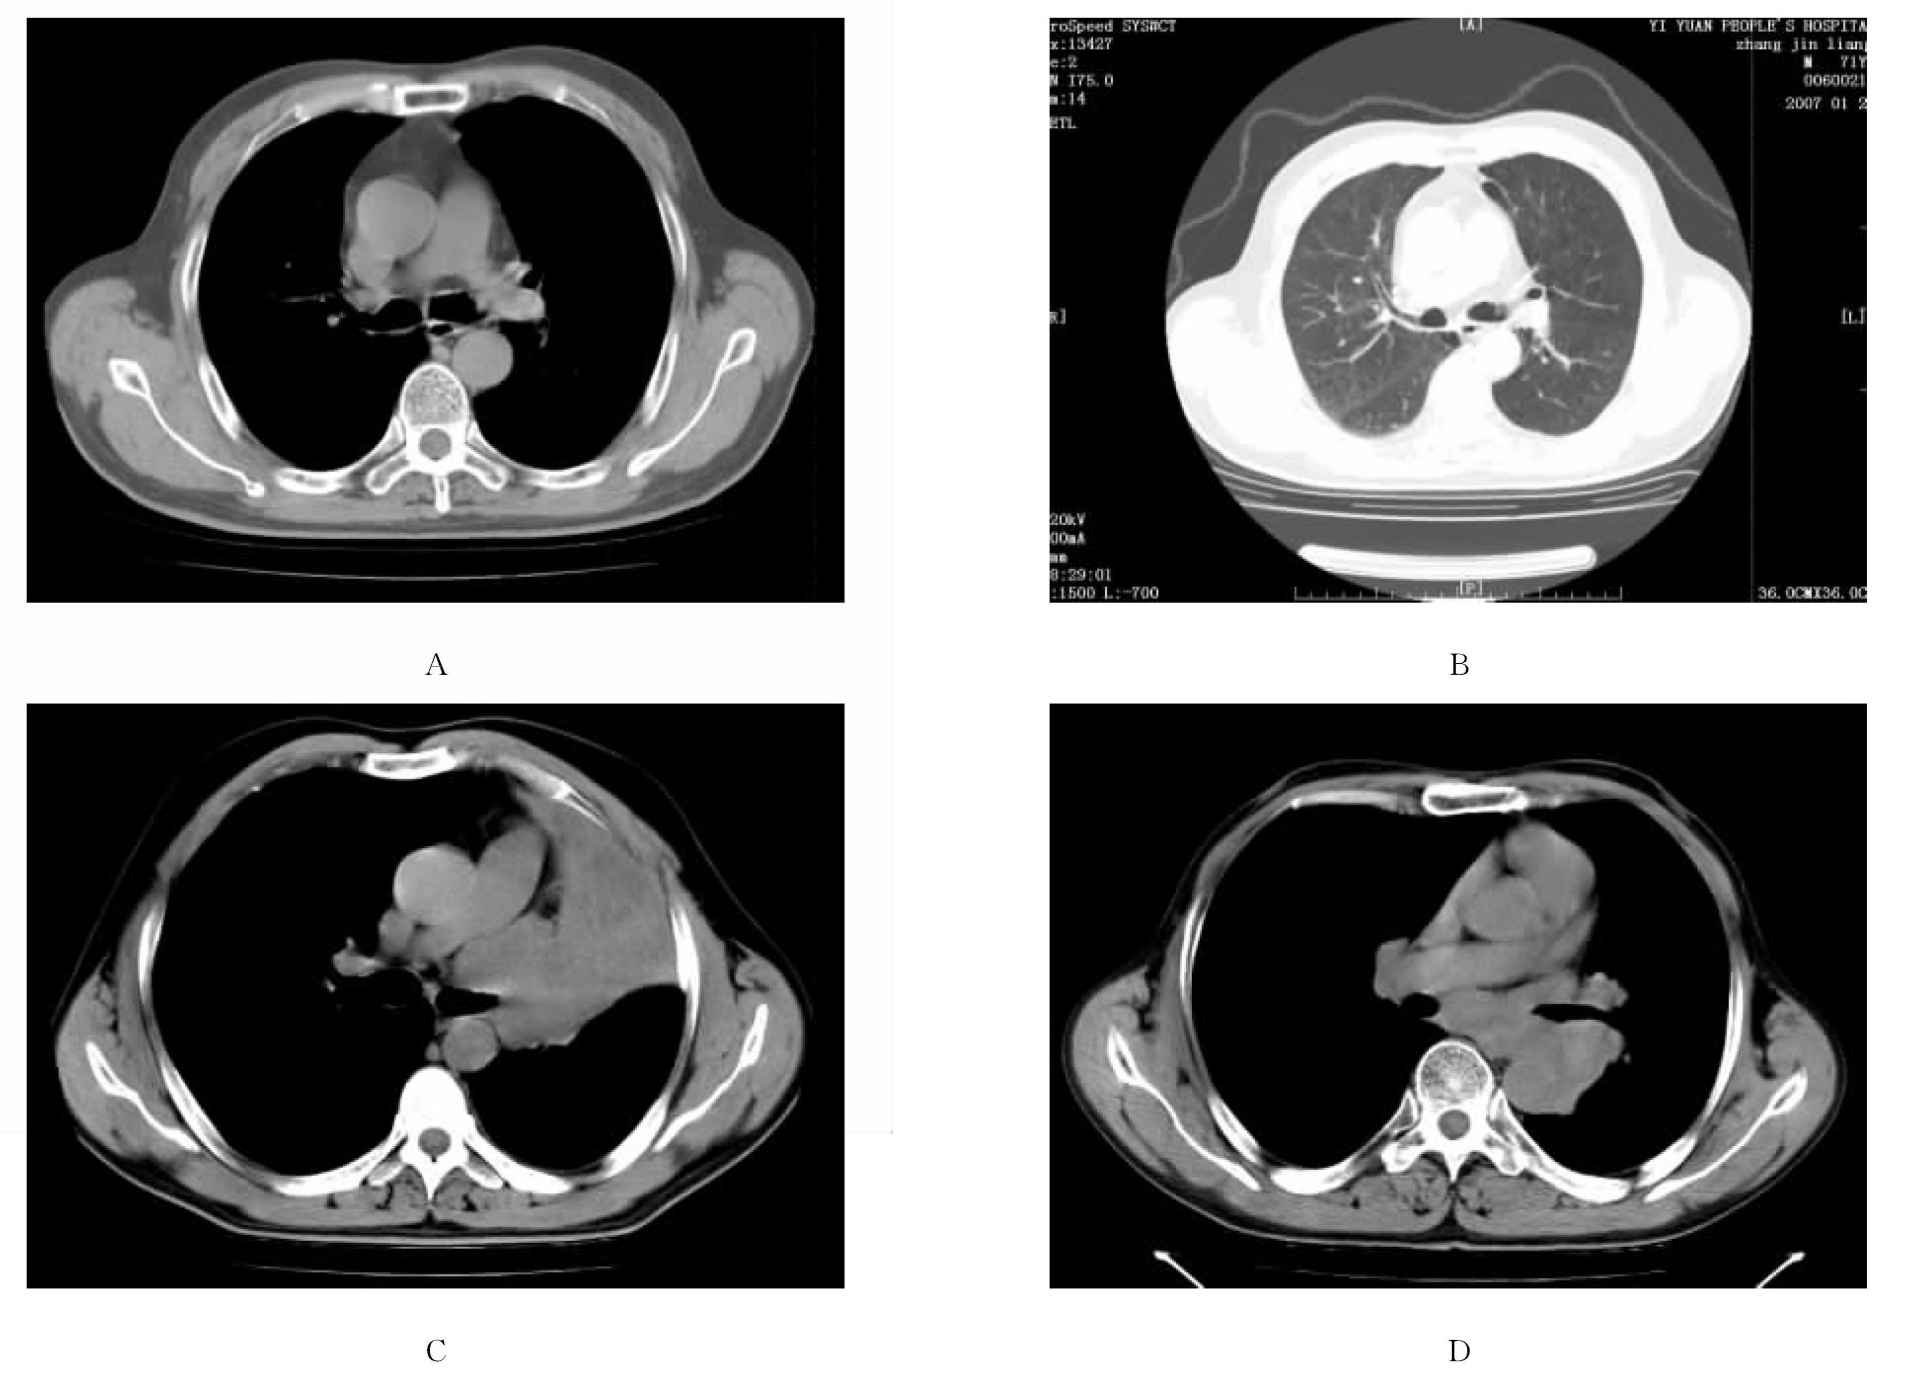
\includegraphics[width=.7\textwidth,height=\textheight,keepaspectratio]{./images/Image00216.jpg}
 \captionsetup{justification=centering}
 \caption{中心型肺癌\\{\small A、B为同一患者。A.左侧主支气管末端有突向腔内的软组织结节,边缘不规则;B.左肺密度减低,为阻塞性气肿表现;C.左上叶中心型肺癌并左上叶肺不张,肺门部有界限不清的软组织肿块,左上叶密实、斜裂弧形前移;D.左下叶中心型肺癌并纵隔(隆突下)淋巴结转移,左肺门肿块包绕胸主动脉生长}}
 \label{fig9-28}
  \end{figure} 

2.增强扫描表现:一般认为:①阻塞性肺炎CT增强扫描,在实变的肺组织中较易发现相对呈高密度强化的中心型肺癌的肿块;②阻塞性肺不张由于肺血管聚集,增强后肺组织的强化明显,可见到相对呈低密度的中心肿块影;③在肺不张或阻塞性肺炎内含黏液(可合并支扩)的支气管未强化,呈低密度条状、Y型、V型或结节影等;④转移的淋巴结强化较弱或有边缘强化,可与血管鉴别。

国外文献认为中心型肺癌的癌块与不张肺组织的强化有一定时差,这种密度差以注射造影剂后40s至2min内扫描最显著。因为不张肺的血供是相对粗大的肺动脉分支为主,且造影剂经静脉团注后,由右心立刻进入肺循环,其循环路线相对短;而肺癌的血供主要是口径相对细小的支气管动脉的分支,且造影剂经肺循环后,要由左心至主动脉,再入支气管动脉,故循环路线相对较长。这样就造成了不张肺与肿瘤的血流灌注的时间差。但应注意肺癌的血供因组织类型及个体差异,其强化幅度和表现多种多样,需综合分析。

此外,增强的早期,在肺实质达峰值前,偶可见阻塞性肺炎或不张肺内的高密度血管影,即CT血管成像征。

\subsubsection{周围型肺癌}

1.平扫表现:主要包括瘤体内部、肿瘤肺交界带和邻近结构的改变(图\ref{fig9-29})。



\begin{figure}[!htbp]
 \centering
 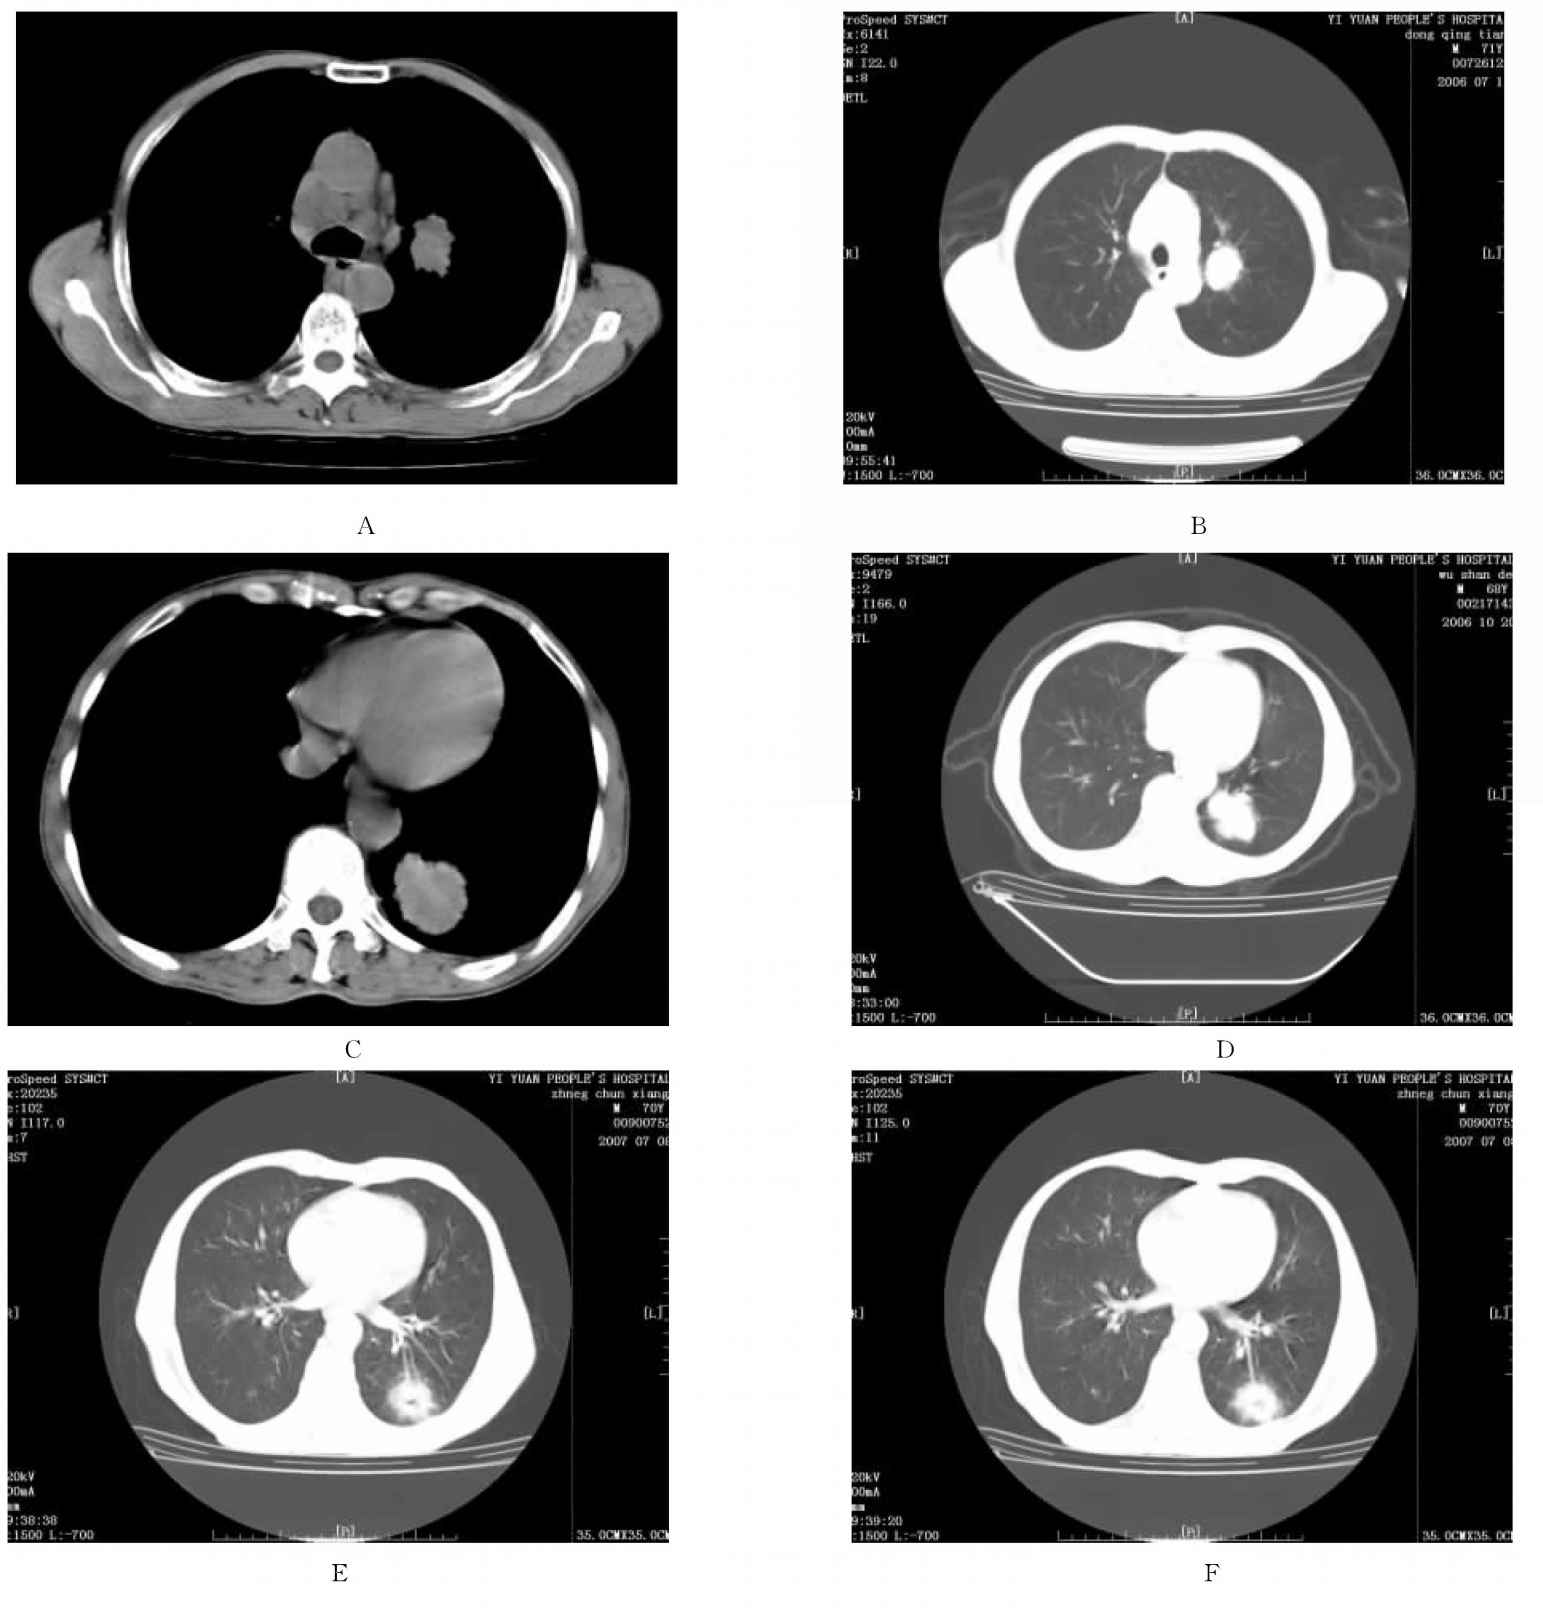
\includegraphics[width=.7\textwidth,height=\textheight,keepaspectratio]{./images/Image00217.jpg}
 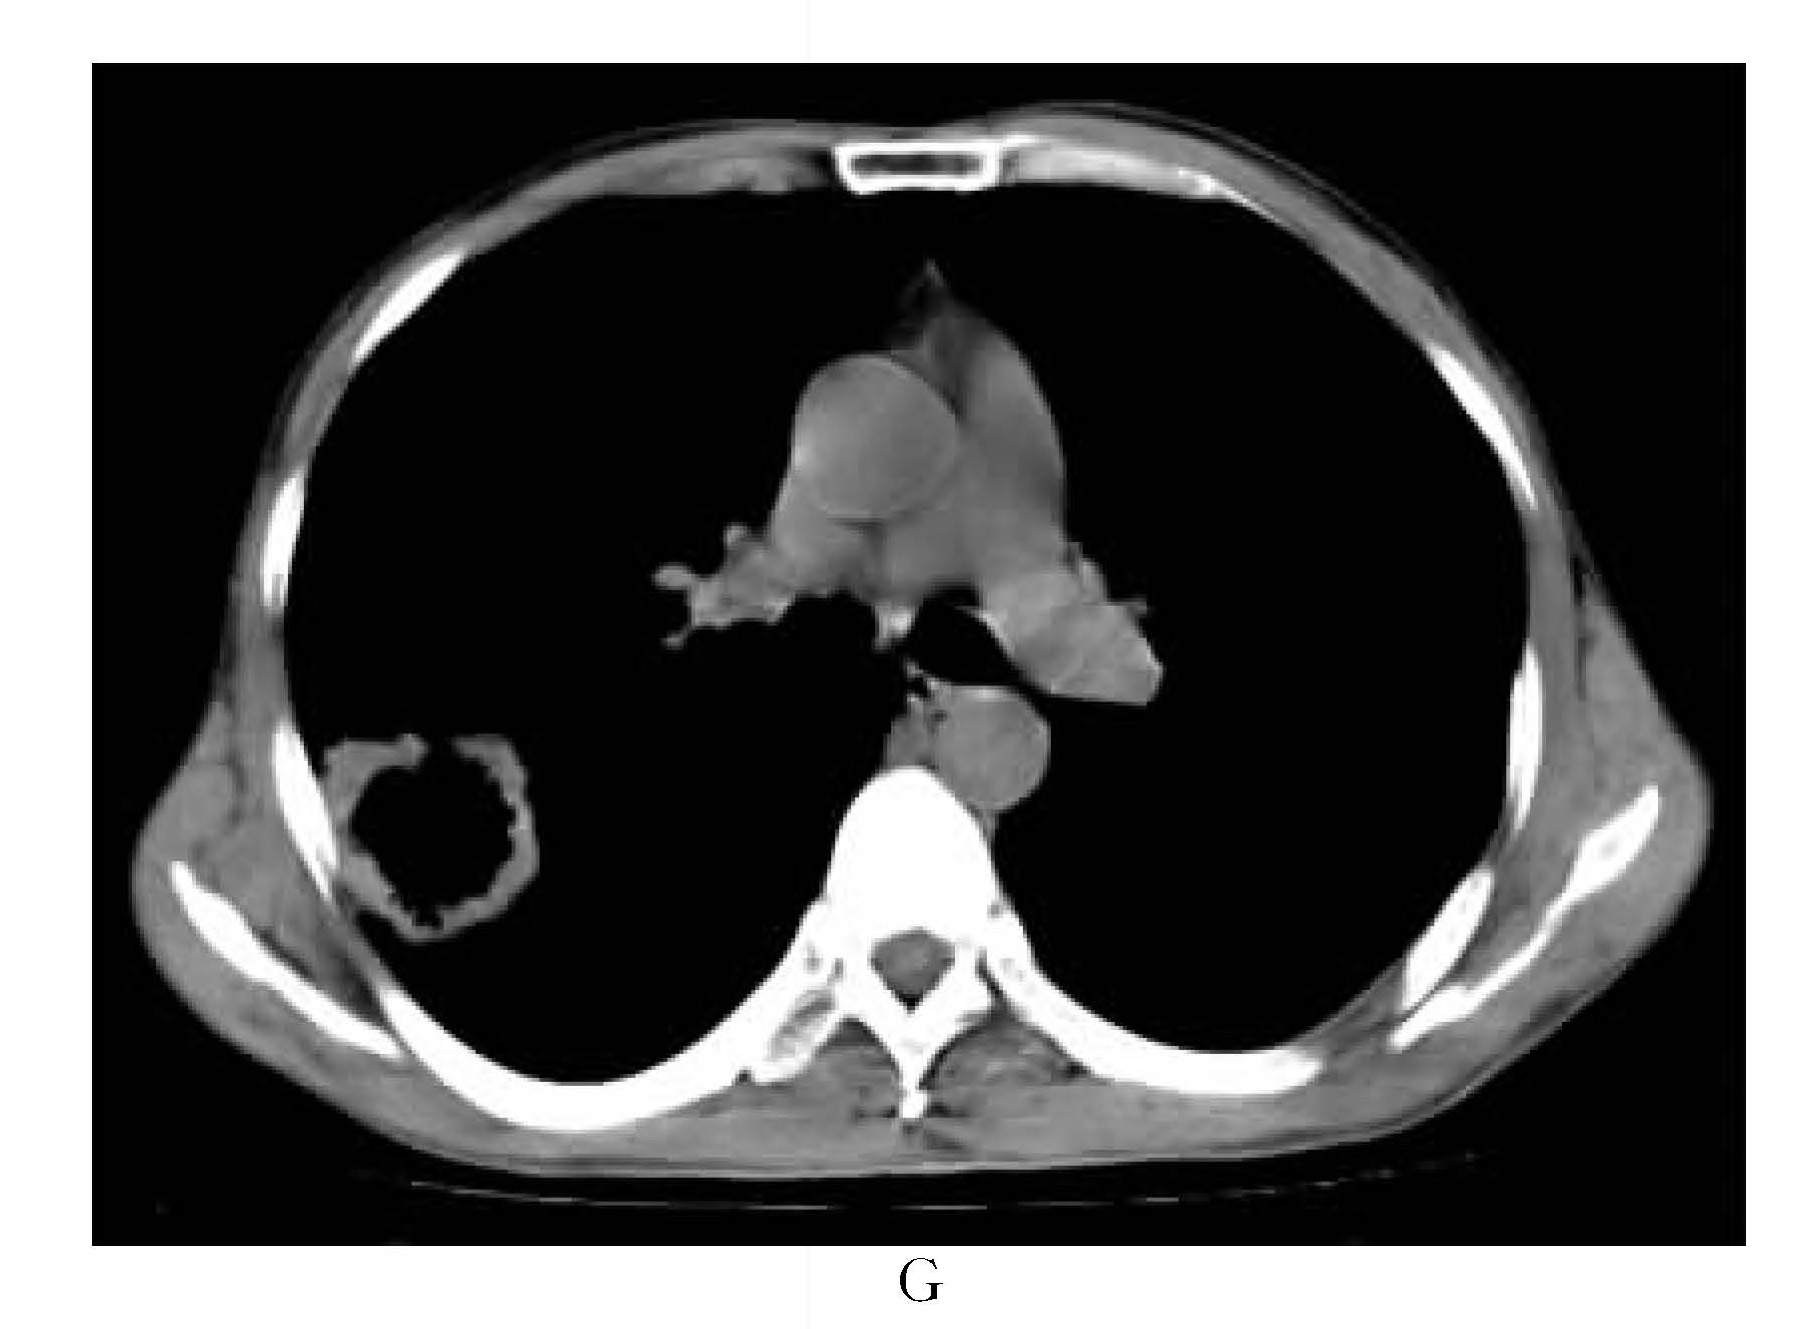
\includegraphics[width=.7\textwidth,height=\textheight,keepaspectratio]{./images/Image00218.jpg}
 \captionsetup{justification=centering}
 \caption{周围型肺癌\\{\small A、B为同一患者,病灶位于左上叶,边缘不规则,有棘状突起和毛刺征;上腔静脉后、主肺动脉窗淋巴结转移。C、D为同一患者,病灶位于左下叶,边缘有分叶征;有胸膜凹陷征。E、F为同一患者,病灶位于左肺下叶,可见血管聚集征和血管通入征。G示右侧癌性空洞,壁厚薄不均}}
 \label{fig9-29}
  \end{figure} 

(1)癌肿的形状:多为圆形或椭圆形,有分叶、脐样切迹、棘状突起者较为典型,如靠近叶间胸膜则局部较扁平。

(2)肿块的大小与倍增时间:一般将肿块最大径≤3cm者称为结节灶,>3cm者称为球形肿块。病灶大小对定性意义不大,>3cm者以恶性多见。但国外有学者报道,15%的恶性结节<1cm,42%<2cm。肿瘤直径增加25%,则其体积增加一倍。肺癌倍增时间多为1.8~10个月,通常小细胞癌约1个月,大细胞癌和鳞癌约2~3个月,腺癌约4~6个月,肺泡癌可长达1~2年。故1个月内迅速增大或24个月内变化不明显的基本可以排除肺癌。但个别情况例外,如癌灶内有出血可“增长”迅速;癌灶亦可许多年生长缓慢,甚至多年大小基本不变。

(3)癌肿的轮廓:大多可见短细、僵直的毛刺。少数呈膨胀性生长、有假包膜形成而光滑锐利。国外有学者报道21%的恶性结节有光整的边缘。

(4)癌肿的密度:<2cm时多密度较低,>2cm时密度较高,其内可有空泡征、支气管充气征等。

(5)癌肿的钙化:HRCT检出率为13.5%,优于常规CT检查(检出率6%~7%)。表现为单个或数个小点状钙化,对诊断无重要意义。

(6)癌肿空洞:周围型肺癌空洞发生率为2%~16%,其中鳞癌占80%,腺癌和大细胞癌占20%;支气管肺泡癌可发生空洞或薄壁囊性病变(单发或多发),小细胞未分化癌一般不发生空洞。肺癌在2cm以下较少发生空洞(2cm以下结节发生空洞以结核多见),4cm以上的肿块发生空洞多见于肺癌。其特点为偏心性厚壁空洞,内壁凹凸不平,外壁呈波浪状或分叶状。少数可为薄壁空洞。此外,壁厚≤4mm的空洞倾向于良性,≥15mm的空洞倾向于恶性。

(7)邻近肺野的改变:①胸膜方向:可见胸膜凹陷征、胸膜下结节之胸膜侧模糊绒毛征,亦可出现小节段性肺炎、肺不张及其炎症和不张后的纤维索条。②肺门方向:经淋巴管向肺门方向浸润转移,形成条索状癌性淋巴管炎。③周围肺野:可见血管纠集征、邻近肺静脉被包绕或中断。此外还可见卫星灶,呈小点或小圆形结节,轮廓清楚,密度较淡。

(8)邻近胸膜、胸壁、纵隔的直接侵犯及纵隔淋巴结转移、胸膜转移和肺内血行转移等表现。

2.增强扫描:其增强所见及与良性病变的区别如下。

(1)强化形态:国外有学者将孤立性肺结节(SPN)的强化形态分为5型。①不强化:增强值<5Hu;②均匀强化;③不均匀强化:病灶内有点条或斑片状不强化或强化更显著区;④周围强化:即中心部分无强化;⑤包膜样强化。

<3cm的肺癌多为均匀强化,少数可以不均匀强化。而>3cm的肺癌多为不均匀强化或因中心坏死而呈周围强化。不强化或包膜状强化见于结核瘤,少数结核瘤可以表现为中心曲线状强化或均匀强化。错构瘤一般不强化。炎性假瘤强化形态多种多样。此外,有人认为增强后结节内尤其边缘部出现点、条状更高密度影(血管)是肺癌的较可靠征象,但仍可见于强化较明显的结核瘤和炎性结节。

(2)时间-密度曲线:肺癌的时间-密度曲线呈抛物线状,即注射对比剂后增强值进行性升高,到达峰值后又缓慢下降。但对于到达峰值的时间报道不一,国外报道2分钟、5分钟、1分钟;国内有报道近2/3为2分钟,近1/3为40秒。可能与所选病例的组织学类型(如腺癌和大细胞癌快于鳞癌)、对比剂用量和注射速度不同(有学者报道注射流率越快峰值出现越早)有关。

国内还有学者报道,炎性结节在注入对比剂后增强值迅速升高,速度高于恶性结节,到达峰值后出现轻微下降,之后又上升到原来的峰值状态或高于原来的峰值,故时间-密度曲线呈小锯齿状或不规则形。此外,炎性结节的强化持续时间比恶性结节长。结核瘤的时间-密度曲线近乎水平的直线。

国内有学者用2.5~3.5ml/s流率、注射100ml造影剂发现,肺癌呈缓慢持续升高型,其强化高峰在75秒;炎性结节呈逐渐上升型,其强化高峰在135秒;结核球呈平坦型,无明显强化高峰。

(3)增强值的大小:有人认为增强值<16Hu为良性结节,16~24Hu为不定性结节,>25Hu高度怀疑恶性,>60Hu多为炎性。亦有人把20~60Hu作为恶性结节的诊断指标。但如中央部坏死或产生黏液的细支气管肺泡癌增强值亦可<16Hu;良性病变(如硬化性血管瘤)增强值亦可>20Hu。还有学者认为炎性结节和恶性结节均可表现为均匀或不均匀强化,两者强化幅度均以20~60Hu多见,其强化幅度无显著差异,即使用上述的峰值出现时间鉴别亦价值有限。

此外,计算SPN强化峰值与相应时刻的主动脉强化值的比值即SPN/AO值作为强化指标。如此值>6%(国内有学者将10%作为指标)则肺癌可能大,明显高于良性结节,但炎症除外。近期有学者报道恶性结节的SPN/AO值(14.27±4.37)%及灌注值(3.02±0.96)ml\textsuperscript{-1}
·min\textsuperscript{-1} ·kg\textsuperscript{-1}
均低于活动性炎性结节(18.51±2.71)%、(6.34±4.39)ml\textsuperscript{-1}
·min\textsuperscript{-1} ·kg\textsuperscript{-1}
,两者增强值的大小无显著差异。

\subsubsection{肺癌转移的常见表现}

1.肺门及纵隔淋巴结转移:很常见。纵隔淋巴结转移侵及膈神经、喉返神经引起相应的症状;累及食管可引起移位、狭窄;压迫气管可引起狭窄。但淋巴结增大并非代表已转移,也可见于良性病变如炎症;淋巴结不大亦并非无转移。一般长径>15mm,短径>10mm代表增大,且长径>20mm常为恶性。

2.肺内转移:见于邻近或对侧肺野,单发或多发,呈粟粒状、结节状或小片状高密度灶。中心型肺癌可显示由肺门向外周放射状的条索影。无论中心型和周围型癌肿沿淋巴管蔓延可见支气管血管束和小叶间隔增厚、毛糙,且合并结节。

3.癌肿可直接侵犯胸膜、胸壁,亦可经淋巴道和血行转移到胸膜。癌肿对胸膜的直接侵犯常不易诊断,但肋骨、胸骨或椎体的破坏、胸壁肿块为最有价值的征象。其次为胸膜外脂肪层模糊,胸膜面的隆起较有价值。胸膜转移最常见为胸腔积液,但肺癌也可阻塞淋巴道引起胸腔积液,故胸腔积液并非胸膜转移的特征表现。胸膜转移亦可表现为多个结节,甚至与弥漫性胸膜间皮瘤类似。

4.纵隔的直接侵犯:有时不易诊断。

5.肺癌的心脏转移:有统计转移至心脏者8%~40%。转移途径有血行、淋巴、直接侵犯。其中心包受累最常见,表现为心包积液或广泛、局限的心包增厚、结节或肿块。

6.肺癌的胸外转移:常见部位有肝(占10%~40%)、肾上腺(18%~38%)、脑(8%~15%)、骨骼(38%)、腹膜后(11%~29%)、肾(16%~23%)等脏器。

\textbf{【鉴别诊断】}

\subsubsection{中心型肺癌}

1.由肺癌引起的肺不张,在出现大片阴影之前,由于支气管的阻塞,使末端小支气管发生分泌物滞留,引起某些小叶不张或阻塞性肺炎。所以当发现一个肺段或一个肺叶范围内出现与支气管走行一致的粗大索条状或斑片状高密度影,不可无根据的诊断肺炎或结核。应注意观察支气管腔内、腔壁情况以免误诊。

2.支气管结核:鉴别两者常有困难。支气管结核的特点是病变范围较长,为环周狭窄,无腔内肿块,同时有肺内与肺门、纵隔淋巴结结核,病人较年轻;但急性期可有不规则狭窄伴管壁增厚。而肺癌支气管狭窄较局限,为偏心性的,有腔内肿块,年龄较大等。

3.支气管内转移瘤:最常见的影像学表现为一叶或单侧肺不张及腔内病灶,与中央型肺癌鉴别困难。也可显示肺门、纵隔淋巴结转移及肺内转移结节。

此外,还需注意与支气管良性肿瘤、结节病、支气管淀粉样变性、Wegener肉芽肿等相鉴别。

\subsubsection{周围型肺癌}

良、恶性结节的诊断与鉴别诊断,应参考以下几个方面(见表\ref{tab9-7})。①部位:结核瘤好发于上叶后段和下叶背段;炎性肿块多位于下叶;恶性肿块多位于上叶前段、右中叶、左上下舌段;②大小;③边缘:如边缘分叶征、毛刺征、棘状突起;④内部表现:空泡征、支气管气相、钙化、空洞;⑤结节周围表现:如血管纠集征及血管穿入、中断征,模糊绒毛征,瘢痕旁肺气肿等;⑥胸膜凹陷征;⑦强化表现;⑧转移表现。

\begin{table}[htbp]
\centering
\caption{周围型肺癌的鉴别诊断}
\label{tab9-7}
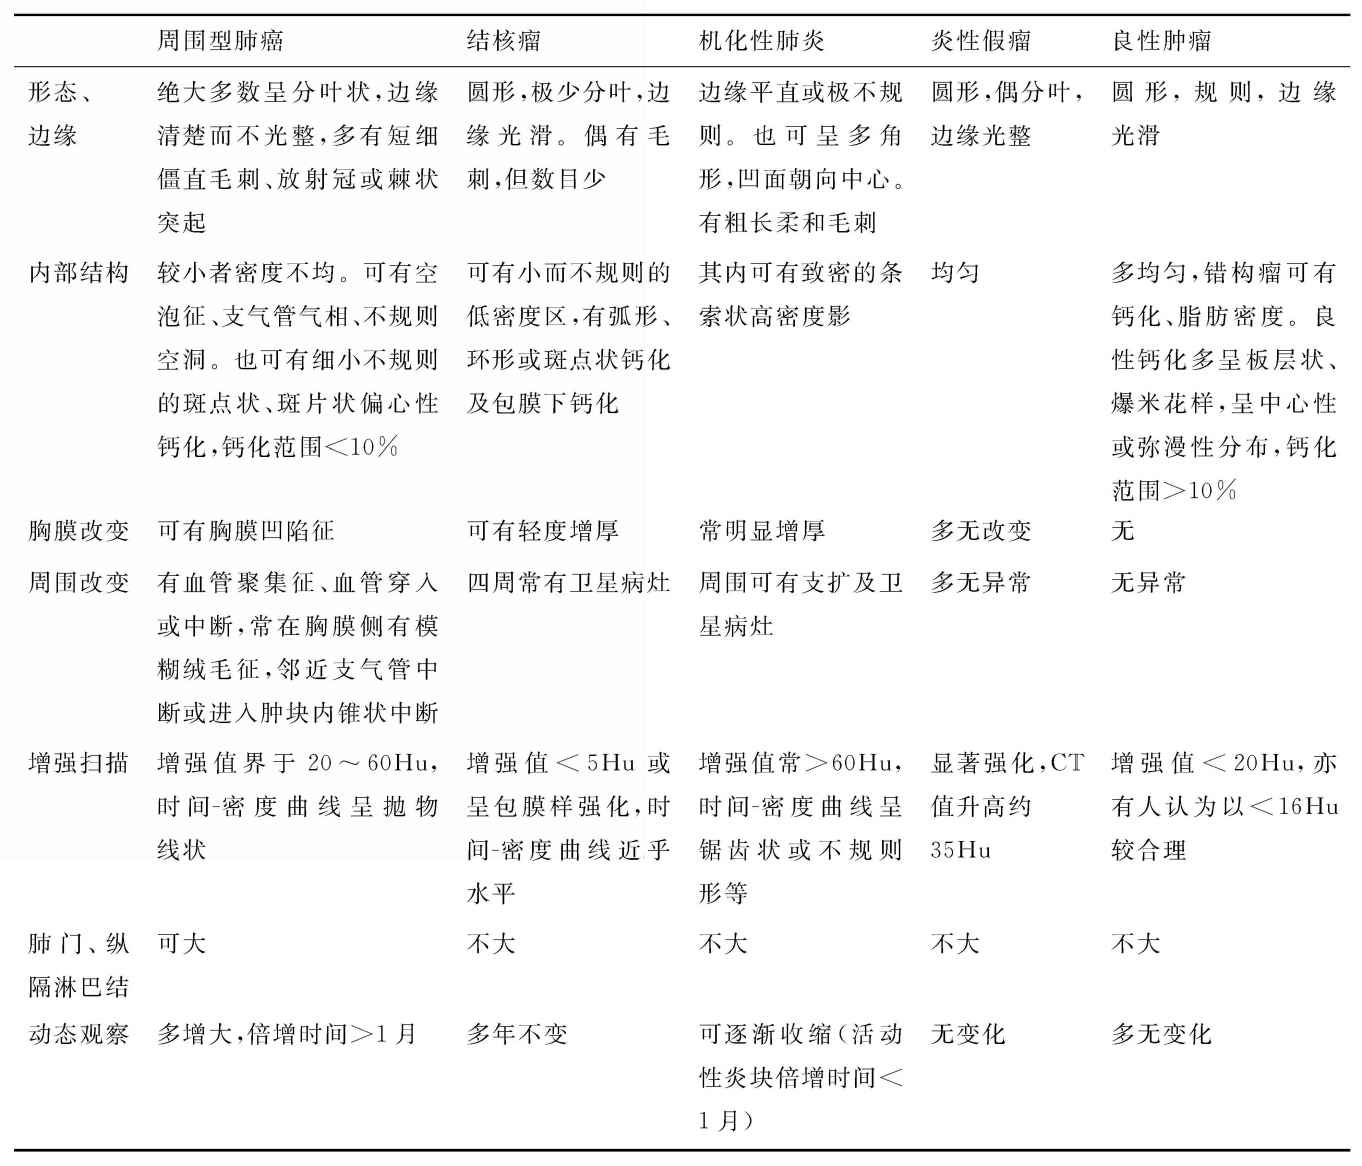
\includegraphics[width=\textwidth,height=\textheight,keepaspectratio]{./images/Image00219.jpg}
\end{table}

\subsection{早期肺癌的CT表现}

1.早期中央型肺癌:分为管内型、管壁型、管外型。在其早期诊断中查痰及纤支镜检查具有重要意义。CT主要表现为肺叶或肺段支气管的增厚狭窄或梗阻,无肺门、纵隔淋巴结转移及远处转移(图\ref{fig9-25}A、B)。但肺癌黏膜下浸润在常规层厚CT和支气管镜检查可为阴性。故薄层CT或HRCT,甚至结合三维重组等检查方式尤为重要。

2.早期周围型肺癌:是指病灶直径≤2cm者,亦有以<3cm为标准者,无肺门、纵隔淋巴结转移及远处转移,亦称为周围型小肺癌。主要表现为空泡征、结节征、边缘分叶征、边缘毛刺征、胸膜凹陷征等。

(1)依瘤体密度分为:①磨玻璃密度结节:呈磨玻璃密度,其CT值<-100Hu。大多为腺癌,特别是高分化腺癌。②部分磨玻璃密度结节:为磨玻璃密度内出现实性高密度的结节性病灶。主要为腺癌,国外有学者统计实性高密度的结节所占病灶的比例<30%者多为恶性,>30%者均为恶性。③实性高密度结节:HRCT上CT值为-100~20Hu,部分表现为软组织密度结节。中心密度均匀或不均匀(甚至有小空洞),常具有毛刺、分叶、胸膜凹陷及周围血管受侵等边缘征象。④空泡征和支气管气像:主要见于腺癌,特别是呈磨玻璃密度的分化好的腺癌。

(2)边缘形态:有人将直径<3.0cm结节的HRCT边缘形态分为6型。①圆形、卵圆形:多为良性肿瘤、转移瘤、感染,极少数为肺癌。②分叶:82%为恶性肿瘤,主要为膨胀性生长。少数为感染病灶,偶见错构瘤,良性肿瘤罕见。③密集毛刺:97%为恶性肿瘤,特别是腺癌,为伏壁式生长。④凹凸不平:呈多发不规则锯齿状,不平整,93%为恶性,主要为伏壁式生长。⑤多角形:凹面朝向结节中心,80%为感染,20%为肺癌。⑥乳晕边缘:结节被磨玻璃密度包绕,基本为恶性,为伏壁式生长。

(3)与周围血管的关系:当肺内结节周围出现血管分支或有血管穿透病灶内部时,高度提示为小腺癌。

\subsection{周围型肺癌的相关CT征象}

\subsubsection{空泡征}

空泡征是指肺癌病灶内散在的、直径≤5mm的低密度气泡,藉此与肺癌空洞鉴别。多见于3cm以下,尤其是2cm以下的肺癌。肺癌有此征象者约占24%~48%,以细支气管肺泡癌和腺癌多见。良性结节中如局限性机化性肺炎、结核球等亦可见及。还有人认为病灶内遍布有多发的小透亮区更符合浸润性病变如消退中的肺炎,但淋巴瘤和细支气管肺泡癌亦可见及。

病理基础:①扩张的呼吸性细支气管及其所属气道;②数个破裂的肺泡融合腔;③瘤组织尚未占据的肺泡腔;④癌组织小灶性坏死,但当坏死组织进一步增多,坏死物大量排出,空泡增大,>5mm时则成为空洞。

\subsubsection{结节征}

结节征是指瘤灶内<5mm的结节状高密度灶。这些小结节如位于病灶边缘可构成分叶。

病理基础:①堆集式生长的肿瘤组织被充气肺组织所衬托;②病灶内肺小叶阻塞性肺不张和肺炎被充气肺组织所衬托。

\subsubsection{多结节聚合征}

国内有学者对肺内球性病灶进行研究发现,部分病灶有多结节聚合表现,并将其分为两型。

1.桑椹样多结节聚合征:有数个或10个左右小结节聚合而成,花瓣状排列,多者可达数10个。他们统计的1组病例中均见于肺癌。该征与常指的分叶征有所不同。其病理基础可能为:①多个小叶间隔的纤维增生阻止了肿瘤生长;②肺癌各部的生长速度不均一;③肺癌生长局部遇到阻力,如血管、瘢痕组织等结构阻挡。

2.宝塔样多结节聚合征:其形成的病理基础为肿瘤以连续浸润方式进行扩散。随肿瘤的不断增大,从原发灶脱落下来的瘤细胞经组织间隙、淋巴管、血管等侵入并破坏周围正常组织,继续生长而形成葫芦状、宝塔状结构。该征多见于分化程度较差的肿瘤。肿瘤无论呈堆积式生长还是伏壁式生长,均可形成此征象。临床上见1例结核有此征,主要为干酪样物质沿支气管向肺门方向蔓延所形成。

\subsubsection{分叶征和脐凹征}

1.分叶征:在肺癌中占25%~76%,形成的主要因素是肿瘤生长速度不均等。此外,肿瘤在不断的向外扩展中遇到的阻力不同;肿瘤突破小叶间隔向外扩展,合并多个小叶间隔,形成了较大的分叶,也是其形成的因素之一。但25%的良性结节,特别是错构瘤其边缘亦可有分叶征。

分叶征深、浅的判断:根据单个分叶的弧弦距与弦长比值大小分为3类。弧弦距/弦长≥0.4为深分叶;等于0.3为中分叶;≤0.2为浅分叶。肺癌多为深分叶。

2.脐凹征:也称脐孔征,癌肿的肺门方向局部凹入,为出入肿块的血管区形成。此征象并非肿瘤所特有,肉芽肿亦可见及。

\subsubsection{毛刺征与放射冠}

1.毛刺征:系指从肺肿块边缘伸出的3~15条不等的毛刺状影,一般分为两类。①粗长毛刺:长而粗,长1~2cm,宽1~2mm,数目不等,呈放射状;②短细毛刺:短而细,长1~5mm,宽1mm。

病理基础:①癌细胞侵袭引起肺间质出血、渗出、纤维化,以及瘤内瘢痕收缩所致的受侵拉直的小血管、小支气管及增厚的小叶间隔。瘤旁粗索条为引流静脉。肺癌的毛刺征多见于中、高度分化的腺癌和鳞癌,其显示率为78%~100%。常呈短细、僵直的多毛刺结节或肿块。②在良性病变中则为炎症或促结缔组织生成的反应。良性结节如机化性肺炎、类脂质肺炎、结核瘤等多呈粗长、柔和的少毛刺结节或肿块。

2.放射冠:系肿块边缘放射状细线影进入邻近气肿带(气肿带宽窄不一)。国外文献认为部分毛刺与肿瘤向肺实质播散有关,而另一些毛刺被认为是肿瘤的促结缔组织增生的纤维带。机化性病变(包括感染和肺梗死机化)、肺结核的纤维空洞外缘也可有类似的边缘特征,因此放射冠不能视为恶性肿瘤的特有征象,但常提示为恶性。

\subsubsection{棘突征}

棘突征亦称为锯齿征,是指球形病灶(包括中央型肺癌)边缘的尖角状排列的数个突起。国内有文献报道其基底宽度最小3mm,最宽10mm,平均6.0mm;高度最小3mm,最高15mm,平均6.6mm。

病理基础:主要为恶性肿瘤细胞向肺内不等速浸润性生长所致,堆积式生长和伏壁式生长均可形成此征。此征以纵隔窗显示为佳。该征肺癌发生率约50%,良性病变亦可见及。

与毛刺征的鉴别:毛刺征在肺窗片上显示清晰,近、远端相差不大,纵隔窗常不易显示,而棘突征则呈棘状突起。如小长三角形,近、远端存在差异,近端宽,远端窄,纵隔窗观察其边缘轮廓清楚,而肺窗则显示边缘模糊。

\subsubsection{含气支气管征}

含气支气管征又称支气管气像或细支气管气像,是指结节内宽度>1.5mm的条状含气影。系癌组织在细支气管和肺泡表面生长而未充填管腔。其CT表现长短不一,有的见分支;非典型者为单个圆形或椭圆形气体密度影,出现于相邻的扫描层面。

该征见于伏壁式生长的肺癌,以腺癌和细支气管肺泡癌出现率最高,亦可见于鳞癌及鳞腺癌。据报道肺癌此征出现率为70%。炎性病变特别是局灶性机化性肺炎亦可见该征。

\subsubsection{血管聚集征和血管通入征、血管支气管平行征}

1.血管聚集征和血管通入征:在部分肺癌,因反应性纤维结缔组织增生显著,可将附近血管牵拉靠向结节或将其卷入结节内形成血管聚集征(亦称纠集征)和血管通入征。其走行僵直,肿块远侧血管可扩张。与炎症所致的走行自然的肺动脉血管增多、增粗之局部充血征象有别。但血管纠集征、血管通入征、肿块远侧的血管扩张征亦可见于炎块,而且也是结核瘤毛刺征的病理基础。

与肺血管的关系:连续系列薄层扫描图上,见肿块邻近肺静脉中断、包绕时常提示恶性结节。因为周围型肺癌直径在3cm左右时,70%以上累及邻近两个肺段或亚段。肺静脉位居肺段或亚肺段的边缘,故易受侵犯。亦有人将肺结节与肺动、静脉的关系分为4型。Ⅰ静脉优势型:肺静脉单独进入结节或比肺动脉粗;Ⅱ肺动脉优势型:肺动脉单独进入结节或比肺静脉粗;Ⅲ无血管进入结节;Ⅳ难以判断。结果95%的Ⅰ型结节为恶性,58%的Ⅱ与Ⅲ型结节为恶性,Ⅳ型中94.4%为恶性。故凡与血管尤其是肺静脉发生关系的结节大多是恶性的。

2.血管支气管平行征:该征由国内学者提出,是指肺内椭圆形或类圆形结节、肿块之长轴与肺门侧血管支气管平行或稍成角(<15°)。在肺窗上表现为同一或连续不同层面,见1支或多支血管支气管与结节或肿块相连,血管在结节、肿块处衔接或被包绕。该征类似于血管通入征,亦多见于肺癌,但偶可见于炎块。

\subsubsection{模糊绒毛征}

该征只能在肺窗观察到,位于球形病灶的周围特别是胸膜侧,呈片状或楔形模糊绒毛样改变。其范围仅局限于球形病灶胸膜缘或前后缘之内。增强时呈均匀或不均匀强化,其内可见粗大的血管影。此征亦可见于结核瘤和炎块。

病理基础:瘤体组织直接压迫或阻塞肺静脉、淋巴管使其回流受阻所致。

此征一般不引起胸膜改变。与短细僵直、大小较均匀、密度较高,围绕肿瘤呈放射状排列且与肿瘤相连的毛刺征有别。

\subsubsection{胸膜凹陷征}

肺内肿块伴发的胸膜改变,通常包括胸膜凹陷、胸膜增厚、胸膜结节和胸水。胸膜凹陷征为结节或肿块与胸膜间的线形、三角形影,周围型肺癌中占49%。

病理基础:其形成的根本原因为肿瘤内反应性纤维化、瘢痕形成。病理组织学表现为肺癌间质中大量成纤维母细胞增生及胶原纤维形成,其收缩作用所致的向心性牵拉主要表现为胸膜凹陷。此外,还受肿瘤-胸壁距离和组织学类型的影响。有胸膜凹陷征者多见肿瘤-胸壁距离较近(≤2.0cm,但>0cm),如肿瘤贴近胸壁或距离过大则不能形成。胸膜凹陷征以腺癌和肺泡癌多见。

CT表现:由于纤维牵拉,使附近的脏层胸膜向内陷形成一个喇叭形空窝并被渗液所充填。顶端指向肿块方向,可与一线状影相连。①当扫描层面与凹入中心平行时,可见典型的三角形或喇叭形影(喇叭颈与线影相连);②当扫描平面偏离中心时线状影分为两条以上,并可与瘤体分开;三角形影可由大变小或分成两个以上;③当扫描平面与凹入中心方向(通常为肺底、肺尖的病灶)垂直时,胸膜凹陷则仅呈条形影;④发生在斜裂者,因肿瘤所在肺段之斜裂的前或后方相邻肺段的代偿性气肿,填入斜裂凹入区域,故只见斜裂局限性弯曲或走行失去连续性;如邻近肺组织不能代偿填入斜裂凹入区,则可形成上述类三角形或喇叭形影。

炎性病变如慢性机化性肺炎和慢性肺脓肿等炎块,虽有大量纤维组织增生,但在急性阶段常导致局部胸膜显著增厚粘连,这就失去了形成胸膜凹陷征的基本条件。但该征还是可以见于结核球和炎块。如果胸膜凹陷征形态不规则、伴广泛胸膜增厚往往是炎性肿块的典型胸膜改变。

\subsubsection{肺癌钙化及与良性病灶的区别}

肺癌钙化的机理可能是:①肺部原有的瘢痕和肉芽组织的钙化被肿瘤包绕;②肿瘤坏死区内营养不良性钙化;③肿瘤自身内分泌功能引起的瘤内钙盐沉积(如黏液腺癌);④肿瘤内所含有的骨性组织。

肺恶性肿瘤钙化的方式:多为细小点状、不规则状、斑片状、偏心性分布,其钙化范围通常小于整个病灶的10%。总之,对于无定形钙化,若钙化越细小、越少,呈细盐或沙砾状,则恶性的倾向越大。

肺良性病灶的钙化方式:多为板层状、爆米花样、包膜下钙化,呈中心性或弥漫性,其钙化范围大于整个病灶的10%。

\subsubsection{肺孤立性良、恶性结节与支气管的关系}

国内有学者将肺孤立性结节(SPN)与支气管的关系分为5型。Ⅰ型:支气管被SPN截断;Ⅱ型:支气管进入SPN,呈锥状中断;Ⅲ型:支气管在SPN内呈长段开放状,并可分叉;Ⅳ型:支气管紧贴SPN边缘走行,管腔形态正常;Ⅴ型:支气管紧贴SPN边缘走行,管腔受压变扁。恶性结节最常见为Ⅰ型,其次为Ⅳ型,Ⅴ型最少见;良性结节最常见为Ⅴ型,其次为Ⅰ型,未见到Ⅱ型。总之,Ⅰ、Ⅱ和Ⅳ型多见于恶性结节;Ⅴ型多见于良性结节;Ⅲ型良性略多见。

SPN与支气管关系的病理基础:①周围型肺癌:以膨胀性生长者,癌细胞增殖、堆积,呈实性压迫、推移邻近肺组织。由于肿瘤为支气管源性,故导致支气管在肿瘤边缘中断。以伏壁式生长者支气管仍保持通畅形成含气支气管征。另外,支气管管壁由外向内的肿瘤浸润、管壁产生的纤维性增殖性反应使支气管管壁增厚、僵硬,加上瘤内成纤维化反应的牵拉,使瘤内支气管不仅未被压扁,反而保持高度的通畅甚至扩张,形成其特有的含气支气管征。②良性结节:其边缘的支气管未受肿瘤的侵犯和成纤维化反应的影响,管壁仍很柔软,易受结节压迫而变扁甚至闭塞。结核球引起的支气管截断是由于后者参与形成包膜。炎块的含气支气管征由肺实质的渗出、实变、机化衬托引起,支气管形态自然,常呈树枝状分叉;管腔内可有分泌物、出血或血栓,使支气管表现为断续状。

\subsection{细支气管肺泡癌}

本病又称为细支气管癌或肺泡癌。它是一种起源于细支气管和肺泡上皮的、分化较好的腺癌,占原发性肺癌的2%~5%。

\textbf{【病理】}
其病理特征是肿瘤细胞沿肺泡壁生长,肺正常结构未被破坏,肿瘤分泌的黏液充满肺泡,故影像学常见支气管气相和空泡征。病理分为肺泡型、乳头型、黏液细胞型和混合型。

\textbf{【临床表现】}
多见于非吸烟人群,女性较多,男女之比1∶1。发病年龄低于其他腺癌。临床以咳大量白色泡沫样痰较常见(40.5%),且多为实变型(91.8%)。其他症状无特异性,极少数(7.1%)无临床症状。

\textbf{【CT表现】}

1.孤立结节型:表现为孤立球形影,密度常不均,可有分叶、毛刺、空泡征和支气管气相、胸膜凹陷征、血管集束征。此外,局灶性磨玻璃样改变较常见,如局灶性磨玻璃样改变内有空泡存在则细支气管肺泡癌的可能性很高。结节内(包括多结节型)可有空洞形成。

结节状细支气管肺泡癌的磨玻璃密度影可分为5种类型。①纯磨玻璃密度结节;②磨玻璃密度结节并发癌性淋巴管炎;③结节为磨玻璃密度和肺实变混合影;④结节周围有磨玻璃晕轮;⑤结节带有肺段以上的磨玻璃密度影。

磨玻璃密度影与肿瘤呈伏壁式生长有关。结节状细支气管肺泡癌带有大面积的磨玻璃状密度影,是一个不良的预后征象,可能预示者一个惰性的肿瘤转变成为一个活跃的肿瘤。广泛的结节周边肿瘤细胞伏壁式生长和支气管播散是其病理基础。

2.实变型:亦称为浸润实变型,占该病的30%。一个叶、段或多个叶、段的实变,常合并小斑片或腺泡结节影。且常见支气管气相和空泡征,甚至细支气管呈树枝状分布,有时可见支气管黏液征。叶间裂呈弧形膨出,亦可见磨玻璃样影,多位于小斑片的周边。血管成像征(造影征)是其CT征象之一。国内还有报道,可呈蜂窝样、多发囊样的浸润实变。

CT血管造影征是指CT增强扫描时,在完全实变的肺叶内或大部实变的肺叶内,可见强化的肺血管分支。此征象的出现需要有两个条件:①病变密度明显低于强化肺血管密度;②病变未严重损害肺血管分支。此征的病理基础为肺泡内液性物质充填、肺泡壁增厚及细胞浸润等病变导致肺组织的实变,但未累及正常细支气管及血管结构。但该征并非细支气管肺泡癌所独有,还可见于呈肺实变的原发型肺淋巴瘤(但其密度较肺泡癌高)、阻塞性肺炎、感染性肺炎(较阻塞性肺炎密度高)。对此征的观察,需强化得当,并用合适的窗宽(300~400Hu)、窗位(-20~0Hu)进行观察。

总之,多发叶、段实变伴“蜂窝征”、血管成像征、叶间裂膨隆和远离实变区的腺泡结节和磨玻璃密度影是弥漫实变型的特征性表现(图\ref{fig9-30})。随访观察磨玻璃密度影和腺泡结节进一步发展为新的肺实变,原来正常的肺区又可见新的磨玻璃密度影和腺泡结节是其动态变化的特点。



\begin{figure}[!htbp]
 \centering
 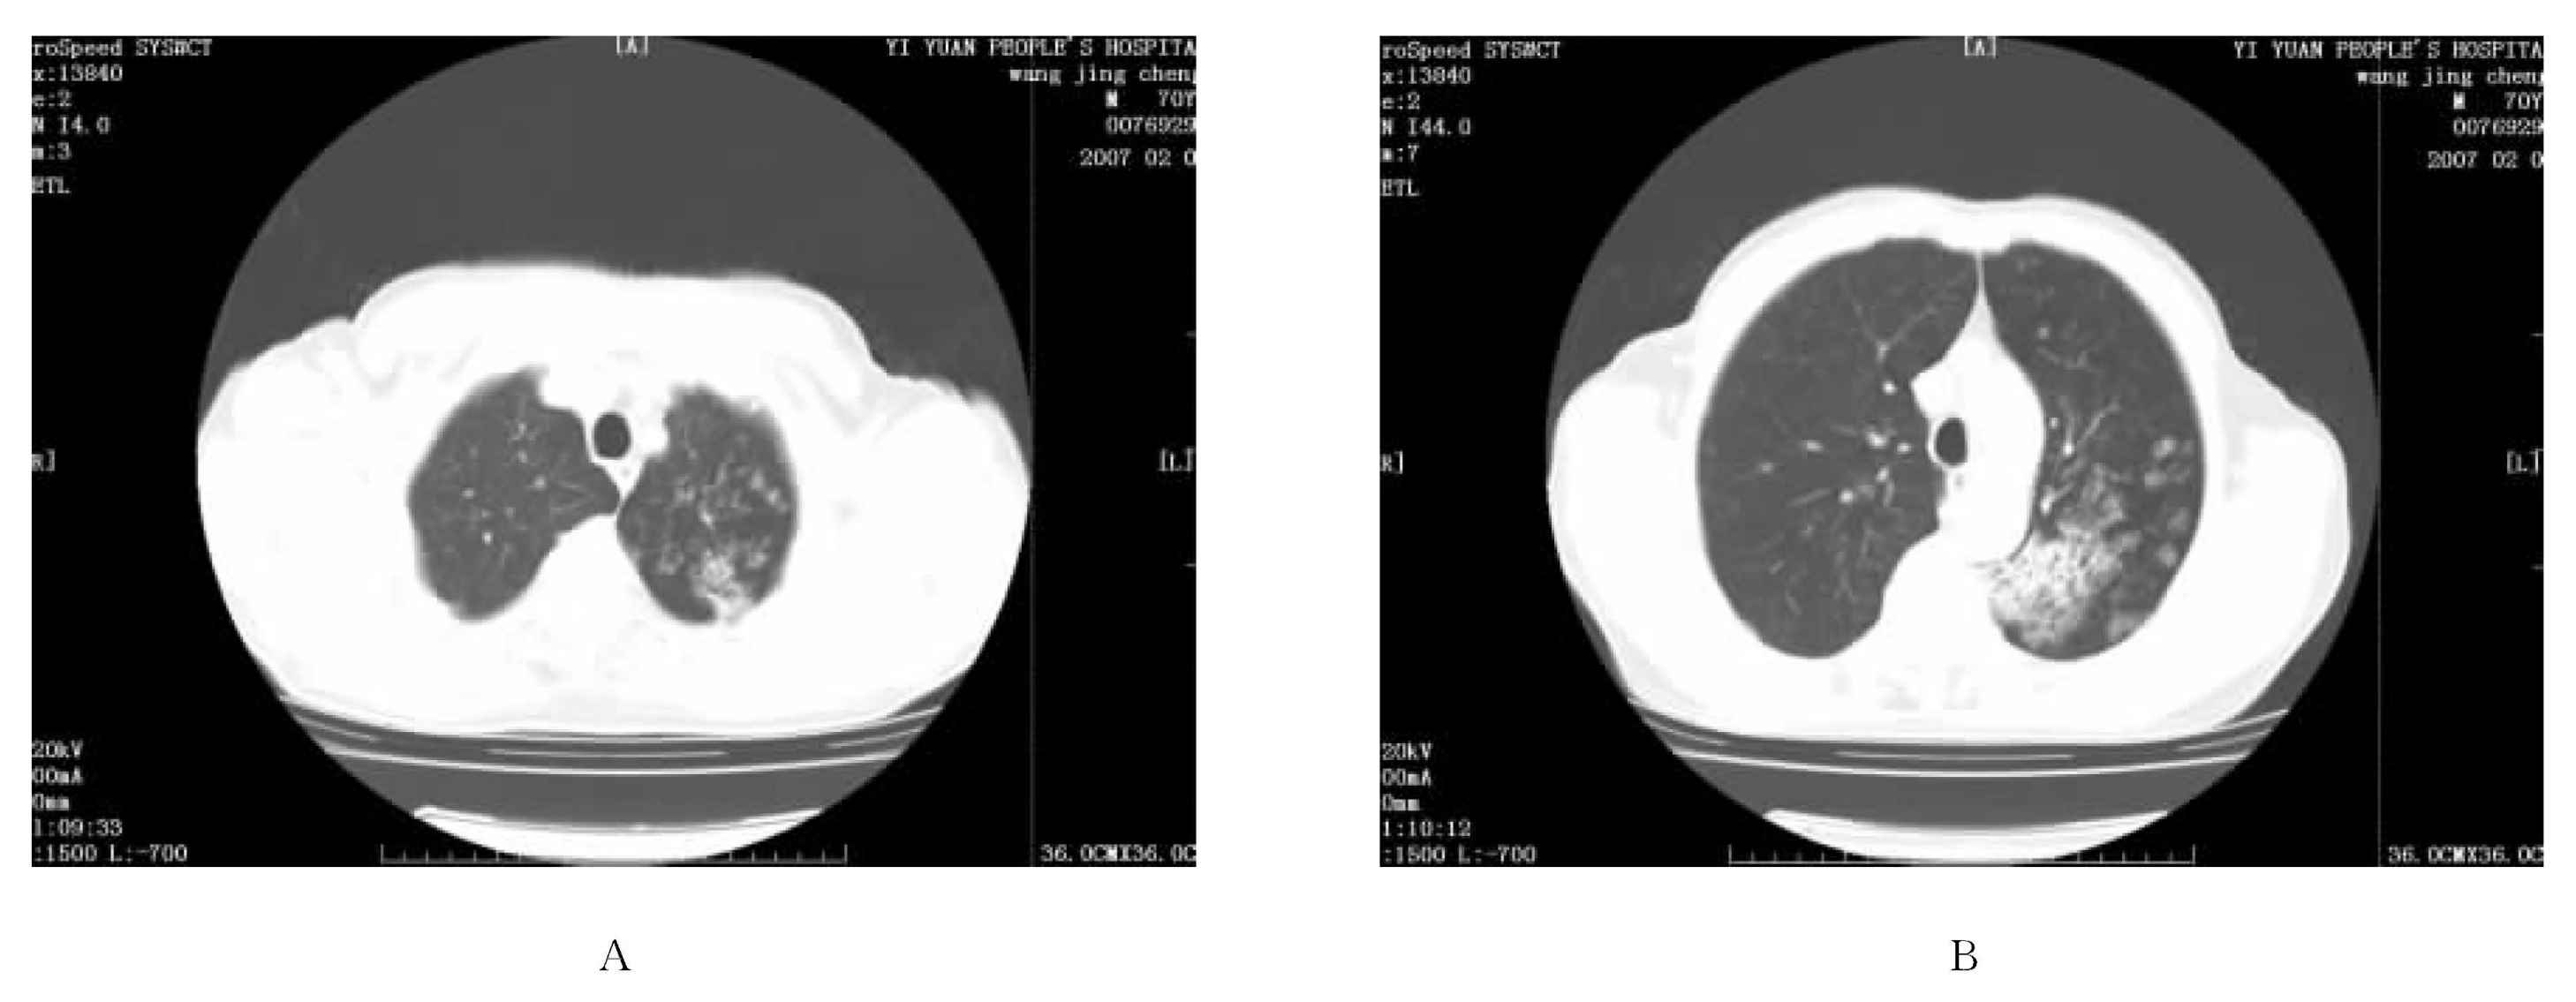
\includegraphics[width=.7\textwidth,height=\textheight,keepaspectratio]{./images/Image00220.jpg}
 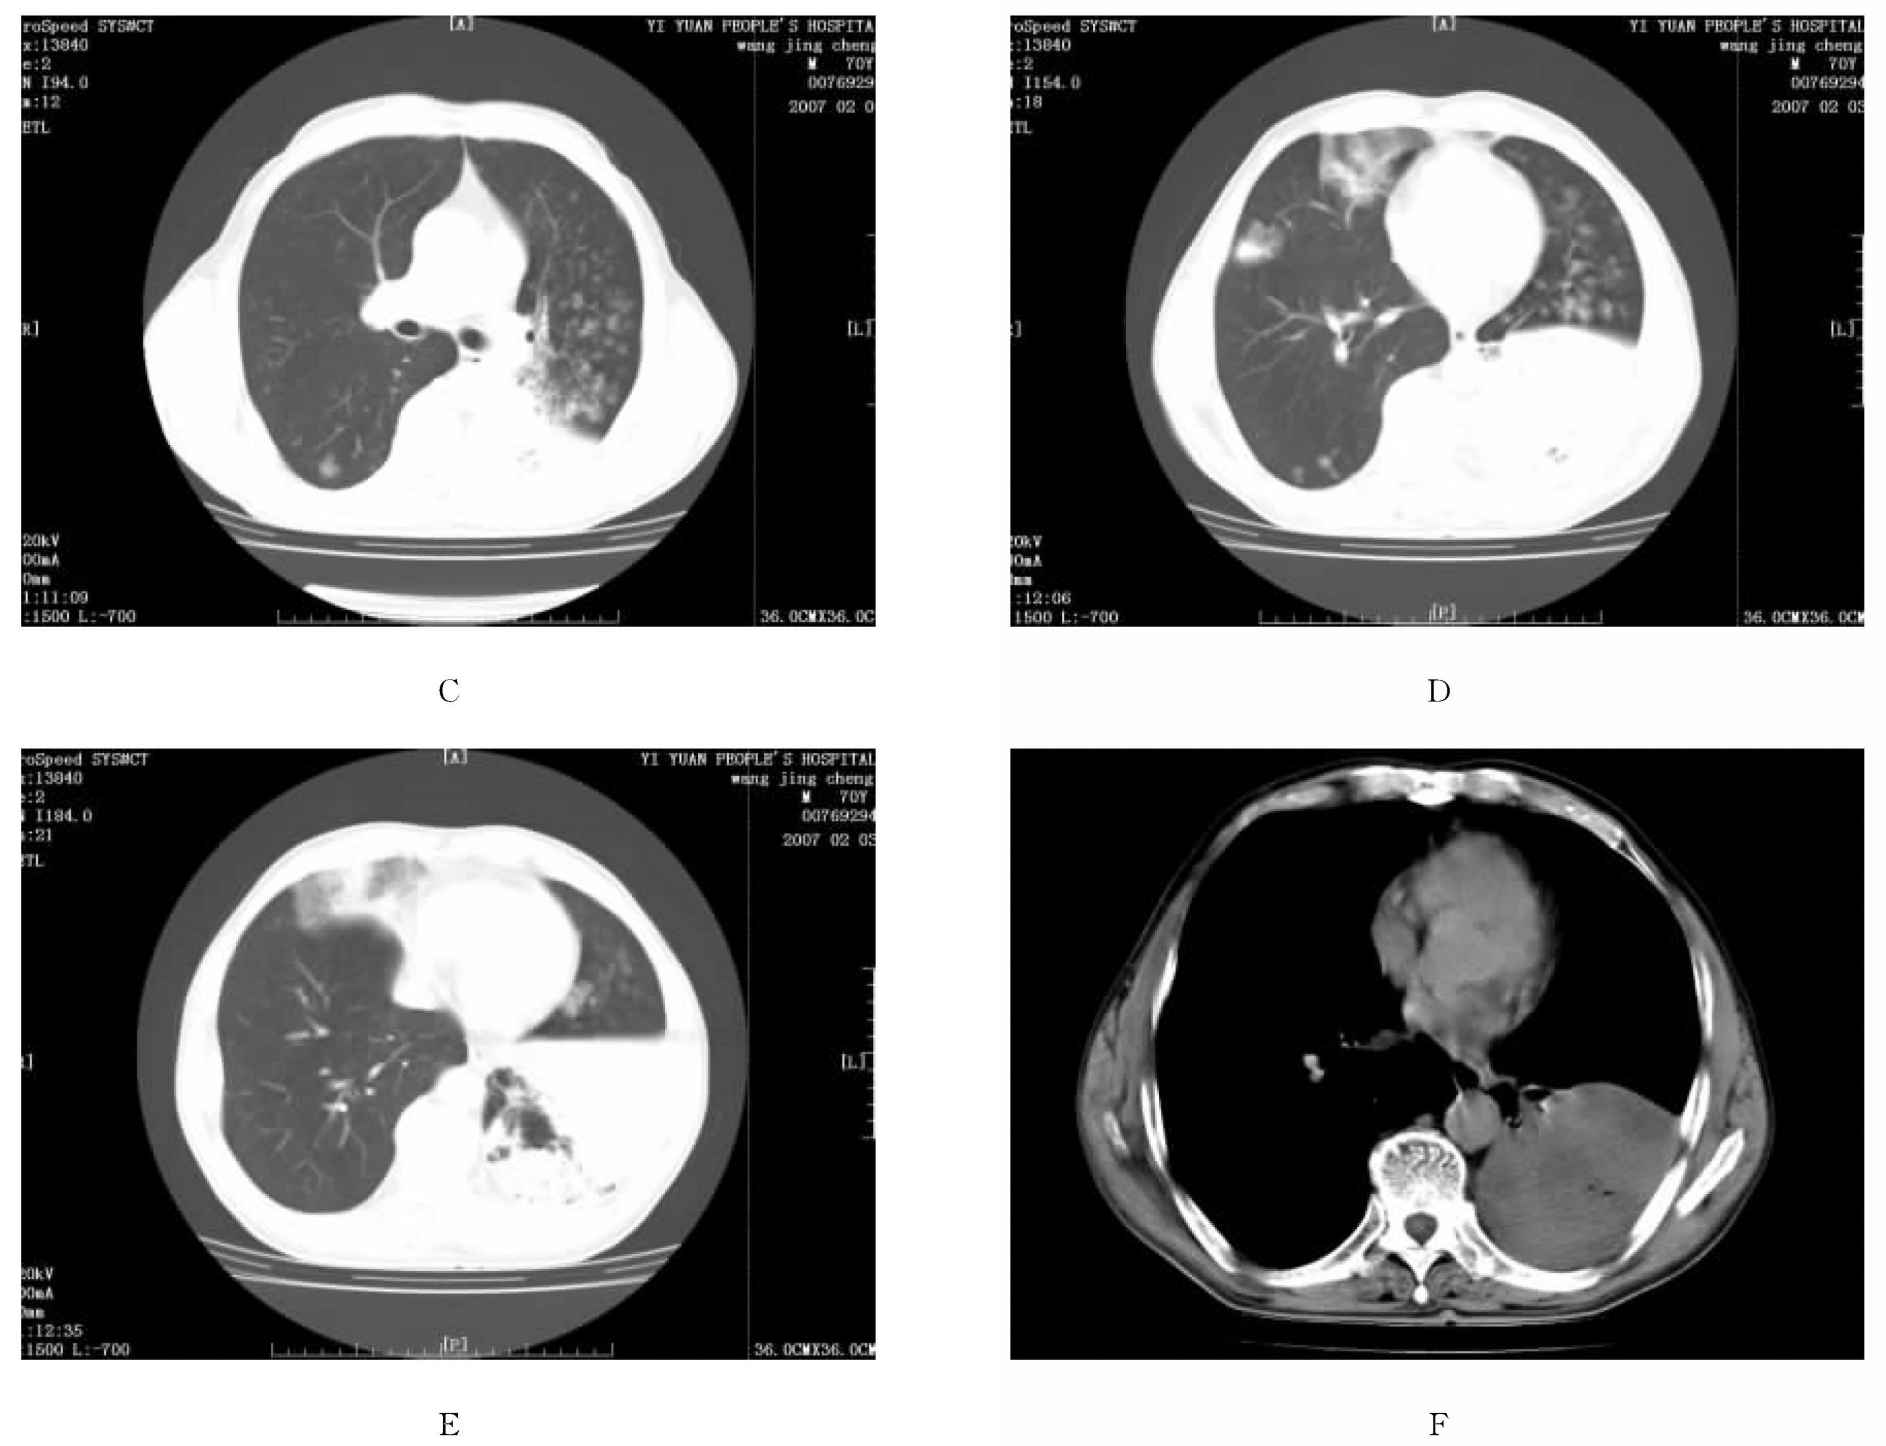
\includegraphics[width=.7\textwidth,height=\textheight,keepaspectratio]{./images/Image00221.jpg}
 \captionsetup{justification=centering}
 \caption{细支气管肺泡癌\\{\small A~F为同一患者,左肺下叶多段实变伴“蜂窝征”(左肺上叶尖后段)、叶间裂膨隆(斜裂)和远离实变区的腺泡结节(左右肺多叶、段)和磨玻璃密度影(右肺中叶)}}
 \label{fig9-30}
  \end{figure} 

实变型需与肺炎、结核、出血、淋巴瘤、肺泡蛋白质沉着症鉴别,但难以鉴别。

3.多结节型:最少见。表现为广泛的细小结节,结节在两肺分布不对称和不均匀。结节可发生空洞或薄壁囊性病变(单发或多发)。结节病灶的融合、以及较大结节或肿块内的支气管气相和空泡征(亦可有钙化)是与粟粒性肺结核和一般粟粒性肺转移瘤的主要鉴别点。

总之,本病进展缓慢。有人认为孤立结节是早期表现,多结节型为实变型的过渡阶段,甚至有人将后两型归为弥漫型。部分孤立结节可数年不变。关于多结节型的发病机制过去认为是肺内转移(淋巴、血行和支气管播散)所致,但也有学者主张克隆学说(认为肿瘤是多起源)。本病可有纵隔淋巴结转移、胸膜侵犯,肺外转移较其他肺癌少见。

\subsection{瘢痕癌}

瘢痕癌是一种特殊类型的周围型肺癌。它起源于支气管黏膜或肺泡上皮,以腺癌多见。一般好发于脏层胸膜下。

1.多数学者认为它是由肺内瘢痕或瘢痕周围的组织演变而成。瘢痕癌附近有陈旧性病灶,以结核病灶为多。早期易误诊为结核。肿瘤的其他影像学表现与其他周围型肺癌无明显区别。

2.另一种学说系肺腺癌生长过程中刺激纤维结缔组织增生,形成显著瘢痕。

\subsection{多源性肺癌}

\textbf{【诊断标准】}
①均为恶性;②每个瘤块相互分离;③具有不同的组织细胞学类型,相同组织细胞学类型者需明确各肿块间无淋巴转移关系或具有各自的转移途径;④无相同组织结构的肺外原发灶证据。

\textbf{【影像学表现】}
①每个肿块有原发癌的影像学表现;②每个肿块相互分离,其间为正常组织;③无肺外原发癌表现;④无淋巴通路的联系,更无淋巴转移表现。

对于两个以上肿块者无法确定是否为多源性,又无法确定哪是原发灶者,可称为多灶性肺癌。

\subsection{肺肉瘤}

本病起源于中胚层组织,发生于肺内者罕见。主要原发于肺间质、支气管和血管壁的基质,并在肺内扩展。有纤维肉瘤、脂肪肉瘤、血管外皮细胞肉瘤、血管内皮细胞肉瘤、恶性淋巴瘤、平滑肌肉瘤、横纹肌肉瘤、骨肉瘤或软骨肉瘤、神经纤维肉瘤、肺母细胞瘤、恶性纤维组织细胞瘤等。其中,纤维肉瘤、恶性淋巴瘤和平滑肌肉瘤占所有肺肉瘤的85%。常为单发,偶可多发。

\textbf{【临床表现】}
本病以40岁左右常见,男性多于女性。症状出现较晚,常有咳嗽、咯痰、咯血和胸痛等症状。痰肿瘤细胞多阴性。

\textbf{【CT表现】} 分为中央型和周围型,但以周围型多见。

1.中央型:表现为肺门附近的肿块向腔内侵犯,引起阻塞性肺不张。也可侵犯局部淋巴结,但很罕见。

2.周围型:①肺周边部肿块:边缘光滑,多有假包膜,密度均匀,常有分叶;②囊腔或空洞形成:因肉瘤生长快,易发生坏死、液化形成囊腔或空洞;③钙化或骨化:因起源于中胚层可有软骨或骨成分;④胸膜侵犯:常见,局部粘连或积液;⑤巨大者压迫肺组织可产生膨胀不全带,支气管可受压移位、变窄;⑥生长迅速;⑦很少发生肺门、纵隔淋巴结转移。

总之,本病无特异性表现,但发现肺内边界清楚、均匀致密或有坏死的,>5cm特别是>10cm的肿块,局部侵犯但无肺门、纵隔淋巴结增大者,应考虑到原发性肉瘤或癌肉瘤可能。特别是合并胸腔积液、肿瘤内钙化及空洞时应考虑到本病。

\subsection{肺淋巴瘤}

\textbf{【定义】}
①单纯发生于肺组织的淋巴瘤,而没有纵隔、肺门和其他部位淋巴瘤者称为肺原发性淋巴瘤。②肺组织内淋巴瘤同时伴有纵隔、肺门淋巴结病变或胸外淋巴瘤者称为继发性淋巴瘤。继发性我国以NHL居多。继发性是由于纵隔、肺门淋巴结病变直接侵犯或淋巴、血行播散所致。

\textbf{【病理】}
原发性肺淋巴瘤罕见,占全身结外淋巴瘤的5%,病理上分为非何杰金淋巴瘤(NHL)和霍奇金病(HD)两类。前者又分为:①起源于支气管相关的淋巴样组织(BALT)的低度恶性小B细胞淋巴瘤;②高度恶性大B细胞淋巴瘤;③血管中心性淋巴瘤(又称淋巴瘤样肉芽肿);④其他罕见类型:血管内淋巴瘤(又称嗜血管性淋巴瘤)。大多数肺原发性淋巴瘤为低度恶性小B细胞淋巴瘤,HD更罕见。

肺原发性淋巴瘤的诊断标准:必须具备以下4点。①影像学显示肺、支气管受累,但未见纵隔淋巴结增大;②以前从未发生过胸外淋巴瘤;③通过临床查体、白细胞计数、腹部同位素、CT或淋巴管造影以及骨髓穿刺等检查,除外了胸外淋巴瘤或淋巴细胞性白血病;④发病后3个月,仍未出现胸外淋巴瘤的征象。

\textbf{【临床表现】}
患者可有咳嗽、咯痰、痰中带血、胸痛、胸闷、发热等症状。原发性者亦可无症状。继发性者还多有全身淋巴结增大,也可有肝脾增大及贫血等症状。

\textbf{【CT表现】}
本病主要侵犯肺的间质和支气管黏膜下组织,支气管保持通畅或有轻度狭窄。

可分为以下6种类型。①肿块结节型:以多发结节多见。可有浅分叶、毛刺征、卫星灶、支气管充气征,有时可形成偏心空洞。②实变型:表现为叶或段的实变,体积一般不缩小。近端支气管狭窄,管腔周围可见增大淋巴结压迫,亦可见腔内小结节。③肺炎肺泡型:可酷似支气管肺炎,甚至与肺结核难以鉴别。有时病变融合成团片状,病变内可见支气管充气征,单侧或双侧发生,与肺水肿或大叶性肺炎相似。④支气管血管淋巴管型:自肺门向外的放射状粗线影或网状结节影。病变在支气管周围侵犯呈线状分布的多发结节,并勾画出气管影。⑤血行播散型:此型较少见,占6%。呈两肺弥漫分布的大小不一的结节或粟粒结节。直径>1cm者可见支气管充气征。⑥心包及胸膜病变:表现为单侧、双侧的心包及胸膜增厚和积液,也可表现为多发的趋向分散的胸膜结节。

此外,继发性一般伴有纵隔、肺门淋巴结增大,同时应注意有无肋骨或胸椎骨质破坏,极少数病例两乳腺增大。部分胸腔积液可能与淋巴管和(或)静脉阻塞有关。大多数病例具有上述两种或两种以上表现。肺淋巴瘤以肺内多发结节多见,且伴有支气管充气征。多发结节的支气管充气征和支气管周围多发小结节勾画出支气管影像被认为是本病的特征性表现。

\textbf{【鉴别诊断】}
本病需注意与癌性淋巴管炎、结节病鉴别。肺淋巴组织增生性疾病除后述的淋巴瘤样肉芽肿和假性淋巴瘤外,还有淋巴样间质肺炎、浆细胞肉芽肿、血管免疫母细胞淋巴结病、巨淋巴结增生病等。影像学均可出现双肺线网状或网状结节影,但又各有其他影像学特点。且肺淋巴增生性疾病与恶性淋巴瘤之间可能存在着由一种良性淋巴增生性病变发展成另一种恶性病变(恶性淋巴瘤)的谱系关系,应予注意。

\subsection{肺淋巴瘤样肉芽肿}

淋巴瘤样肉芽肿于1972年由Liebow等首次提出,它是由血管中心性淋巴组织增生和血管炎性浸润所引起。有人认为可能是血管中心性T淋巴瘤的变异,故又称为血管中心性淋巴瘤(原发性)。但亦有人认为是一种B细胞淋巴组织增生异常,还有人认为是Wegener肉芽肿的变型。确诊需靠病理,其病理特点是血管中心性淋巴细胞浸润。

\textbf{【临床表现】}
本病好发于男性。病变进展快,首先累及肺,还可累及皮肤、中枢神经系统和肾,预后差。主要表现为咳嗽、呼吸困难、胸痛、发热等。

\textbf{【CT表现】}
①双侧多发的结节状、肿块状病灶,边缘模糊呈绒毛状,大小为0.5~8.0cm,常有融合,多位于下肺。近1/5呈单侧肺内结节,常合并坏死、空洞。②由血管炎引起的病变可形成片状高密度灶,其内可见含气支气管征。③病变累及胸膜时可出现胸水。④肺门和纵隔淋巴结增大较少见。

文献报道,也可表现为含支气管气像的肺实变,或仅表现为纵隔淋巴结增大而无肺内异常。总之,对有上述肺部临床症状,病情反复,经抗炎、抗结核治疗效果不佳,同时影像学见两肺实变影,其间可见含气支气管和肺内结节时,应考虑到本病。

\textbf{【鉴别诊断】}
Wegener肉芽肿和坏死性结节病样肉芽肿可有上述类似的影像表现。但Wegener肉芽肿90%有鼻部等上呼吸道受累表现,有助于鉴别;坏死性结节病样肉芽肿女性多见,常有肺门淋巴结增大,肺外侵犯罕见。

\subsection{肺假性淋巴瘤}

本病于1963年由Saltzsein首先提出。通常认为是一种良性炎性淋巴细胞浸润,但随着免疫组化的发展,现被认为是低度恶性淋巴瘤。

\textbf{【病理】}
其病理特征是以成熟的小型淋巴细胞为主的炎性细胞浸润,有生发中心,形成淋巴滤泡。不侵犯支气管壁、胸膜、肺门和纵隔淋巴结。

\textbf{【临床表现】} 该病多见于女性,常无临床症状。

\textbf{【CT表现】}
边界不清的斑片状高密度灶、累及叶或段的大片实变,通常位于胸膜下,其内可见支气管充气征。很少出现空洞、钙化、淋巴结增大和胸腔积液,偶表现为多发结节或浸润。

由于低度恶性小B细胞淋巴瘤的临床预后好,组织学上亦有反应滤泡,因此极易误诊为假性淋巴瘤。确诊和鉴别依靠免疫组化染色或基因表型分析。

\subsection{Kaposi肉瘤}

本病又称为特发性多发性出血性肉瘤、多发性出血性肉瘤等。由Kaposi于1872年首先发现。本病主要见于非洲、次为欧美,亚洲非常少见。主要侵犯皮肤,部分累及内脏。肉眼所见为两侧对称发展的皮肤结节及浸润斑,多呈紫褐色。全身脏器均可受累,较常见的部位为胃肠道、肺部、深部淋巴结等。

\textbf{【分类】}
本病分流行性和非流行性两大类。流行性见于AIDS病人的晚期。非流行性包括3种类型。①经典型:即Kaposi于1872年以“皮肤特发性多发性色素性肉瘤”为名首先报道的病例类型。多为老年人,常继发于恶性肿瘤如淋巴瘤等。病变主要为发生于足部的红蓝色结节,组织学特征为血管增生、出血和含铁血黄素沉着。②非洲型:亦称地区性,男性青年黑人多见。其特点是播散性,淋巴结增大、且迅速坏死。③免疫抑制剂诱发型:表明与免疫功能障碍有关。

\textbf{【病理】}
组织学通常包含交错的纺锤状细胞索,在网状或胶原纤维网中存在脉管结构。该脉管构成裂隙状,红细胞常从血管壁渗出。在纺锤细胞之间还可有含铁血黄素沉着,且可被巨噬细胞吞噬,故肿瘤中常有巨噬细胞、淋巴细胞和浆细胞浸润。

\textbf{【临床表现】}
多见于中老年男性。临床上约有25%的Kaposi肉瘤患者有肺部受累,常发生于皮肤或黏膜Kaposi肉瘤之后。皮肤可见红斑、斑块、皮下结节,多呈紫褐色。可伴有发热,肺部受累可有咳嗽、咳血等症状。

\textbf{【胸部影像学特点】}
①沿肺血管分布的多发性肺内结节,也可呈网格结节状改变或斑片状浸润。其病理基础是肺泡内多发融合的紫色结节和小叶间隔增厚。结节通常边缘模糊,间质改变亦较毛糙。少见的表现为网状浸润影,单发病变罕见。②AIDS病人胸水出现率为35%~63%,且多为两侧。③胸内淋巴结可增大。

此外,同位素扫描亦有助于诊断(病灶摄取铊),并可作为疗效随访的手段之一。

\subsection{白血病}

\textbf{【病理】}
白血病在肺部以肺间质浸润为主。白血病细胞侵及肺泡间隔,使毛细血管与肺泡壁分离。白血病细胞沿支气管、血管周围浸润。

\textbf{【临床表现】}
肺部症状有咳嗽、咯痰和咯血,往往是由于肺部感染所致。

\textbf{【影像学表现】}
①最多见的是双侧性纵隔和肺门淋巴结增大,约占25%;②两肺广泛的网状影或网状结节影,类似淋巴转移;③肺泡内浸润可呈斑片状、大片状实变;④两肺多发的圆形结节,通常为肺栓塞所引起;⑤局部大面积的肺实变,通常由于感染所致(除细菌外,还有真菌、卡氏肺囊虫感染等);⑥胸膜增厚或胸腔积液,占25%,可为单侧或双侧,多由于淋巴阻塞、心衰或感染所致;⑦心影增大;⑧肺出血呈斑点状或大片状。

白血病胸部浸润的CT尤其HRCT表现多种多样,主要为小间隔增厚、外周支气管血管间质增厚、结节影、磨玻璃状改变、气腔实变等。即主要为间质性改变,但无特异性,需与其他并发症鉴别。

\subsection{肺转移瘤}

\textbf{【病因病理】}

1.血行转移:几乎全身所有部位的肿瘤均可转移入肺,而以血供丰富直接回流到体静脉的肿瘤最多见,如甲状腺癌、肝癌、肾癌、成骨肉瘤、滋养细胞癌、子宫内膜癌、黑色素瘤等,其次为胃肠癌。瘤栓到达肺小动脉及毛细血管后,可浸润并穿过血管壁,在周围间质和肺泡内生长,形成肺转移瘤。

2.淋巴转移:全身恶性肿瘤均可通过淋巴转移至肺,最常见于胃癌、胰腺癌、卵巢癌、前列腺癌、甲状腺癌、乳腺癌及肺癌等。其转移机制为:①离心性:即肿瘤细胞先转移至纵隔淋巴结,再沿淋巴管逆行转移到肺门淋巴结、肺内淋巴结和淋巴管;②向心性:即肿瘤细胞经血行转移到肺内,然后经淋巴管转移到纵隔淋巴结。淋巴道转移是肿瘤细胞穿过血管壁侵入周围淋巴管,形成多发的小结节病灶。

3.气管或支气管内转移:即经气管或支气管内膜播散转移。以原发性肺癌尤以细支气管肺泡癌最多见。肺外恶性肿瘤如乳腺癌、肾癌、肾上腺癌、甲状腺癌、结肠癌、恶性黑色素瘤和某些肉瘤亦可经血行和(或)淋巴转移至气管或支气管黏膜下,尤以乳腺癌多见。

4.直接浸润或蔓延:较少见,由胸壁、胸膜、纵隔或膈下的恶性肿瘤直接侵及蔓延至肺。

\textbf{【临床表现】}
多数先有原发肿瘤的症状和体征,也有些病人缺乏原发肿瘤的临床表现。肺转移瘤病变较轻微的病人可无任何症状。主要表现为咳嗽、呼吸困难、胸闷、咯血和胸痛等。

\textbf{【CT表现】}

1.血行转移瘤

可为单发的、多发的和大量弥漫、随机分布的圆形病灶或粟粒性病灶(图\ref{fig9-31}A、B)。①孤立性肺转移:约占血行转移瘤的5%。多见于结肠癌特别是乙状结肠癌,其次是骨肉瘤、睾丸恶性肿瘤和乳腺癌以及黑色素瘤。肿瘤通常密度均匀,边缘清晰光滑,无毛刺征、分叶征或分叶不明显。个别轮廓模糊、或有分叶和毛刺。②多发性肺转移:占血行转移瘤的60%以上。呈球形,边缘光滑、清楚,密度均匀,大小不一,以两中、下肺多见。③数量极多的多发转移和粟粒性肺转移:多见于血供丰富的原发癌如肾癌、甲状腺癌、肝癌、骨肉瘤及滋养细胞癌等。表现为两肺密布的结节或细小结节。

总之,②、③两种转移方式结节大小不一,系多次血行转移的结果,在肺野内由上至下呈逐渐增多、增大的趋势,并多位于肺表面。此外,肺转移瘤多生长缓慢,但绒癌和骨肉瘤肺转移例外。少数结节因伴发出血表现为“晕轮征”。

2.淋巴性转移瘤

淋巴管炎样表现且常伴肺门淋巴结增大是肺淋巴性转移瘤的常见表现。①从肺门向肺野呈放射状分布的树枝状或索条状影,通常位于肺的一侧或一叶,甚至一段(图\ref{fig9-31}C、D)。HRCT可见肺门区支气管血管束增粗呈结节状;小叶间隔或胸膜下间质呈串珠状或均匀增粗,小叶中央支气管血管束增粗呈结节状。②病变发展后,约50%可见肺门甚至纵隔淋巴结进行性增大。有些病例较早出现纵隔(或)和肺门淋巴结增大,代表离心性转移方式。③常有胸腔积液,积液为淋巴回流受阻或胸膜转移所致。④有时可同时存在血行转移改变。

\begin{figure}[!htbp]
 \centering
 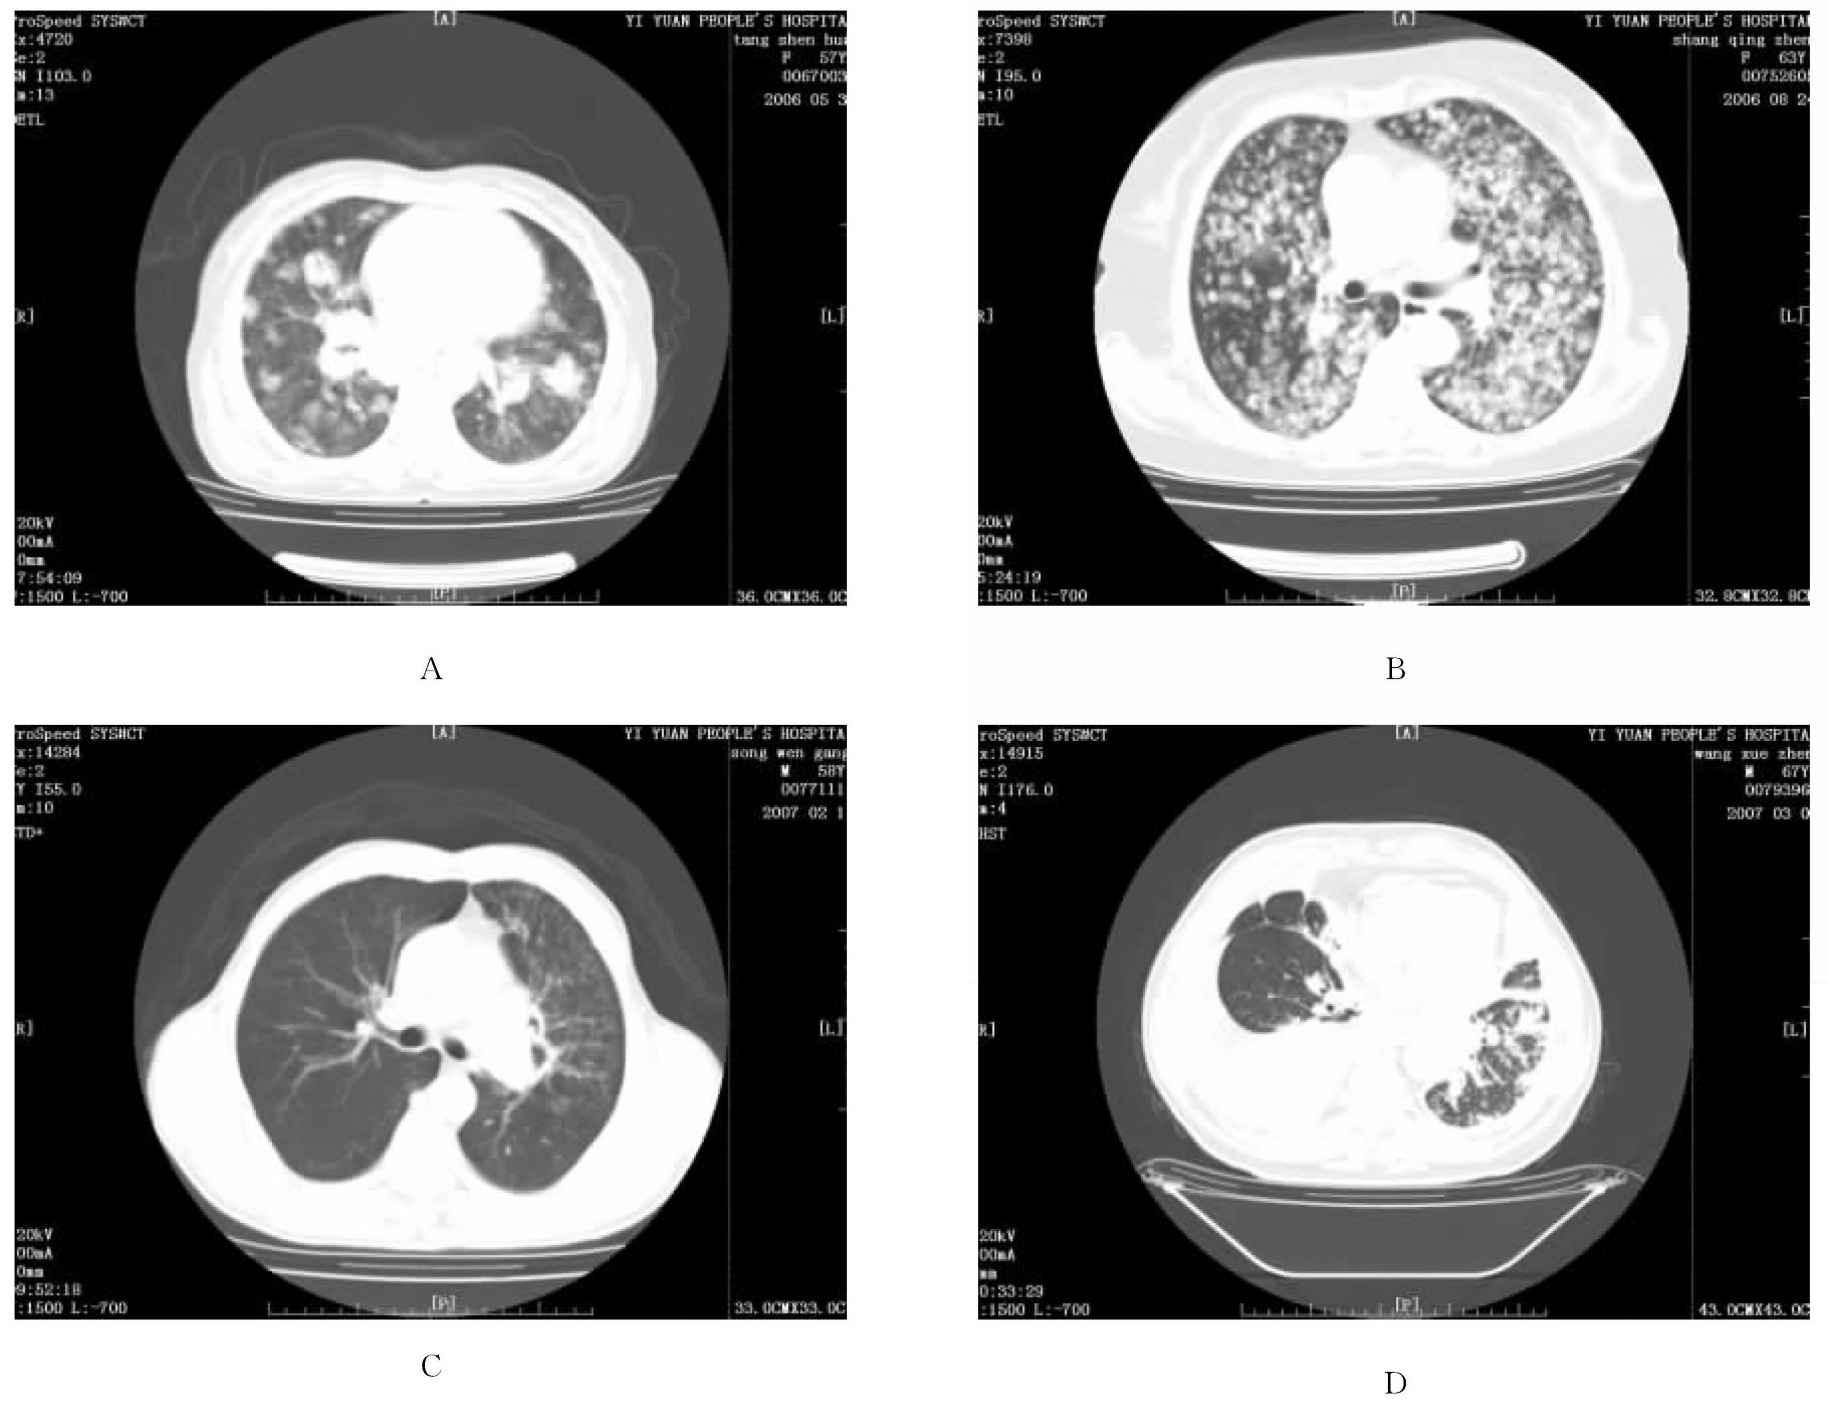
\includegraphics[width=.7\textwidth,height=\textheight,keepaspectratio]{./images/Image00222.jpg}
 \captionsetup{justification=centering}
 \caption{肺转移瘤\\{\small A、B非同一患者,为双肺血行转移瘤,有大量弥漫性分布的高密度结节;C、D非同一患者,均为左肺癌并左肺淋巴性转移瘤,分别可见左肺上叶和下叶支气管血管束增粗,边缘不规则}}
 \label{fig9-31}
  \end{figure} 

3.非典型表现

(1)空洞及空泡样转移:腺癌和鳞癌发生空洞性转移的多见,且两者发生机率无显著差异,转移性肉瘤亦可。多为不规则厚壁空洞。有报道空洞壁厚度<4mm
者最多,洞壁厚度均匀者亦较多,而且鳞癌洞壁中壁厚度均匀者多于腺癌;囊样空洞似仅见于鳞癌。其形成原因与放疗、化疗或原发灶切除有关。空洞及空泡样转移的形成机制可能是肿瘤坏死或向支气管内侵犯形成活瓣所致。与肺真菌病等鉴别困难。

(2)钙化:可见于骨肉瘤、软骨肉瘤、滑膜肉瘤、骨巨细胞瘤、结肠癌、卵巢癌、乳腺癌、甲状腺癌的肺转移和经治疗的转移性绒癌。

(3)瘤周出血:表现为结节周围出现磨玻璃样密度或边缘模糊的晕(晕征),但晕征不具有特异性。以绒癌和血管肉瘤肺转移多见。此外,黑色素瘤肺转移亦可见边缘模糊,甚至类似肺炎。

(4)自发性气胸:少见,文献报道以骨肉瘤的肺转移最常见。

(5)类似肺炎等的含气间隙实变:腺癌的肺内转移可类似肺泡癌,沿完整的肺泡壁在肺内蔓延。影像学表现似肺炎,可表现为含气间隙结节、伴含气支气管征的实变、局灶或弥漫的磨玻璃密度、伴晕征的肺结节。可见于乳腺癌、胃肠道腺癌和卵巢腺癌的肺转移。

(6)肿瘤栓塞:CT表现为周围亚段肺动脉分支多处局限性扩张、串珠样改变,并可见肺梗死所致的楔形实变影。CT和肺动脉造影可发现段以上动脉内的较大血栓。原发癌常见于肝癌、乳腺癌、肾癌、前列腺癌和绒癌。

(7)支气管内膜转移:发生率低,仅见于2%的病例。表现为肺叶或一侧性肺不张,CT还可见支气管内膜转移灶。与原发性肺癌不易鉴别。

(8)单发转移:有胸外恶性肿瘤的病人,发生单发肺结节时25%~46%为转移瘤。

(9)瘤内血管扩张:增强扫描肺转移结节内有时可见扩张、扭曲的管状强化,为肿瘤血管。常见于肉瘤如平滑肌肉瘤。

(10)灭活转移瘤:有些转移性肺结节经充分化疗后大小不变或轻微变小,手术切除后发现为坏死性结节伴或不伴纤维化,无存活的肿瘤细胞,称为灭活性转移瘤。常见于绒癌、睾丸癌转移化疗后。但影像学不易确诊。

(11)良性肿瘤肺转移:罕见。常来源于子宫平滑肌瘤、葡萄胎、骨巨细胞瘤、成软骨细胞瘤、唾液腺多形性腺瘤和脑膜瘤。影像学上难与恶性肿瘤肺转移相区分。

\subsection{小结}

\subsubsection{肺癌组织学类型的影像学判断}

1.中央型:①中央型肺癌以鳞癌和小细胞癌为主,而腺癌和大细胞癌均少见。②中央管内型多为鳞癌,鳞癌多表现为管腔内息肉状菜花样突起,常表现为阻塞性肺不张。③中央管外型多为小细胞癌。④中央管壁型肿瘤同时累及肺叶和肺段支气管,支气管呈不则狭窄或突然截断,肺内阻塞变化较明显时以鳞癌多见。⑤中央管壁型肺癌累及肺段支气管,纵隔和肺门淋巴结增大,支气管呈规则狭窄或锥形梗阻,肺内阻塞变化轻或无阻塞变化时,以小细胞癌多见。总之,小细胞肺癌以中心型为主,呈实性生长,密度较均匀,易侵犯支气管及纵隔大血管,伴肺门及纵隔淋巴结转移。

2.周围型:①肺炎样肺癌:无论是局限性还是弥漫性,多为腺癌和肺泡癌。②肿块<3cm,有空泡征、胸膜凹陷征、支气管气相,且边缘模糊者多为腺癌及细支气管肺泡癌。③肿块>6cm,累及段支气管,肿块中有空洞,且肿块边缘较清楚者,以鳞癌多见。④其余周围型肺癌中,小细胞癌和大细胞癌(肿块较大,以膨胀性生长为主,边缘清楚)特点不明显。

\subsubsection{肺恶性肿瘤并发气胸的机制}

①肺外周或胸膜下的肿瘤结节发生坏死,形成支气管胸膜瘘,从而导致气胸;②瘤结节造成支气管不完全阻塞,使远侧的肺泡过度膨胀而破裂,气体沿小叶间隔到达胸膜下,形成胸膜下疱,后者破入胸腔而形成气胸;③患有慢支、哮喘、肺气肿的老年患者的气肿大泡支架易受癌肿破坏而断裂;或代偿肿瘤所致的肺不张,使已高度膨胀的肺泡最终破裂。

气胸为肿瘤的晚期并发症之一。对显性肺肿瘤出现气胸表明病变已进展到晚期;对已知患肿瘤的病人,出现气胸提示有肺转移的可能;肺肿瘤并发气胸者80%为转移性肺肿瘤。

\subsubsection{肺癌和肺转移瘤形成薄壁空洞的机制}

①当肿瘤长在小气管内并起到活瓣作用时,其远端气腔膨胀扩大,以后支气管内的肿瘤逐渐长入气腔壁内;②肿瘤结节先形成空洞,以后由于小气管内肿瘤的活瓣作用,使空洞壁变得更薄。

李铁一等观察到薄如囊肿的肺癌空洞,经病理证实有两种情况。①病灶溶解形成薄壁空洞;②先天性肺囊肿引起恶变。转移瘤所致的薄壁空洞(甚至呈空泡样转移)多与肺内其他结节灶并存。

\subsubsection{肺部孤立性结节诊断的注意问题}

孤立性肺结节(SPN)是指一个不伴有肺不张和淋巴结肿大,直径<3cm的圆形或类圆形的实性病变。其鉴别诊断很广,最终诊断常需做活检。

1.病因有感染性、炎症性、血管性、外伤性和先天性疾病及肿瘤,其他的良性病变有类风湿结节、肺内淋巴结、肉芽肿和结节病。虽多为良性,但原发肿瘤约占35%,孤立性转移瘤也不少。

2.要注意分析病灶的位置、形态、边缘、密度及周围肺野的改变。

3.一个结节大约经历了30次倍增才达到1cm直径。有人预算在X线能见之前,大部分肺癌已存在8~10年。对肺癌来说迅速生长是不可能的(肺癌倍增时间多为1.8~10个月,但小细胞未分化癌的倍增时间可为1个月),即使转移亦不可能。但有些侵袭性很大的转移瘤(如骨肉瘤、绒癌)可迅速生长。生长很慢的结节,如18个月以上直径增大1倍者提示为良性病变(如错构瘤,其他尚有类癌、炎性假瘤或肉芽肿)。但缓慢生长的结节难以排除恶性肿瘤。

4.肺炎和肺梗死动态观察体积常缩小。结合临床可以断定为机化性肺炎、梗死或转移。

5.对动静脉畸形和肺静脉曲张,根据其形态和位置并结合增强扫描,可以提示诊断。

6.肿块靠近胸膜,但不伴胸膜改变者,提示肿瘤(良性或恶性)比炎症病变的机会大。

7.钙化的形式可有利于定性诊断。

8.在一个边缘光滑或分叶的SPN中见到脂肪说明为良性结节,肺错构瘤为其代表。

9.空洞可见于恶性肿瘤(尤其鳞癌),亦可见于炎症性疾病(如脓肿)、感染性肉芽肿、Wegener肉芽肿和肺梗死。壁厚5~15mm者73%为良性结节;壁厚<5mm者95%为良性;>15mm者84%为恶性。

\subsubsection{多发性肺结节和肿块诊断的注意问题}

1.多发性结节与多灶性浸润的区别在于:结节的密度均匀而且边缘清晰;界限不清是浸润病变的较为固定的概念。

2.多发性肺结节最常见的病因是转移性疾病。多发性结节和空洞形成强烈提示转移瘤可能,亦可见于Wegener肉芽肿、类风湿性肺病、真菌病(周围多有胸膜增厚、纤维瘢痕等感染征象)。肺的空洞性转移,男性最可能来自头颈部,女性多来自生殖系统。

3.向肺内转移的原发肿瘤很多,但中枢神经系统肿瘤极少导致肺转移(血脑屏障破坏后亦可转移至肺)。

4.出现钙化虽可见于良性肉芽肿,但一个肉芽肿出现钙化并不能证明其他结节都是良性肉芽肿。

5.大的多灶性境界不清的阴影,经过几周或几月后,结节变小、边缘清晰,提示结节为肉芽肿愈合或肺梗死机化等。这一演变过程可排除转移。

6.怀疑肺部结节为寄生虫病者,结合病史诊断很重要。

\subsubsection{肺结节内钙化对病变的定性价值}

肺结节钙化是具有一定特征的。来自骨肉瘤的钙化易被普通X线所发现,但原发性肺部肿瘤的微细钙化X线平片极为罕见,CT尤其薄层扫描易于发现。

诊断标准:①良性钙化应超过结节横断面积的10%;②钙化必须有对称的沉积式样(如弥漫性、成层的或中央性);③良性结节边缘光滑;④良性结节直径多<3cm;⑤符合以上标准的结节,在24个月随访中不应有变化。

总之,在肿块中央出现向心性漩涡样钙化或全部钙化,实际上已可诊断为肉芽肿;在病变周围出现的偏心钙化,尤其细小砂粒状钙化不应当作良性病变的指征。对多发结节如发现一个结节有钙化,对第二个结节的评价无意义。

\subsubsection{局限性磨玻璃样密度灶}

局限性磨玻璃样密度灶即肺窗上表现为局限性云雾状高密度灶,病灶内血管和支气管纹理仍清晰可辨;纵隔窗上病灶往往不能显示或仅能显示磨玻璃样病灶中的实性成分。根据HRCT特征,孤立性肺结节可分为3型,即纯磨玻璃样密度灶、混合性磨玻璃样密度灶及实性结节。纯磨玻璃样密度灶表现为边缘清楚的均一半透明密度,而混合性磨玻璃样密度灶呈现为磨玻璃样病灶伴有中央结节状、条状、片状、带状致密影。局限性磨玻璃样密度灶可有多种病变引起,包括炎症性病变、局限性纤维化、腺癌和不典型腺瘤样增生(AHH)等。

局灶性机化性肺炎(病理上相当于肺间质纤维化和慢性炎性细胞渗出区域,并混杂有肺泡内的水螅样肉芽组织)在HRCT上可表现为明显持久的局限性磨玻璃样密度灶,这些病灶可能被误为细支气管肺泡癌。炎症和结核随访有吸收或纤维化改变是鉴别诊断的关键,随访数月稳定的局限性磨玻璃状密度灶很可能是早期肺腺癌或AAH。炎性结节、AAH或局限性细支气管肺泡癌周围往往见不到放射状的线样高密度影。

AAH常常呈现为纯磨玻璃状密度灶,而细支气管肺泡癌或腺癌在纯磨玻璃状密度灶和混合性磨玻璃状密度灶的出现率相近。因此根据局限性磨玻璃样密度灶内实性成分的多少在一定程度上可以鉴别肺腺癌和AHH。

国外有学者认为,≤10mm并伴有磨玻璃密度成分的结节与恶性有明显相关性(88%的混合性磨玻璃样密度灶为恶性,而无磨玻璃成分的结节恶性者仅为30%)。而且国外还有学者研究认为磨玻璃样密度的比例越大,肿瘤的侵袭性越小、复发率越低。亦有学者发现周围型肺腺癌HRCT表现为局限性磨玻璃样密度灶和实性密度,前者生长缓慢,后者呈现为快速生长。有清楚边缘和含气腔隙的局灶性磨玻璃样密度灶或以磨玻璃样密度为主的病灶很可能是肿瘤性病变。≥10mm的纯磨玻璃样密度灶或混合性磨玻璃样密度灶是恶性的重要征象。恶性病变往往密度不均,内部可见实性成分,毛刺、分叶征象和胸膜凹陷征、支气管征、含气腔隙常见于恶性肿瘤。肺纤维化不具备毛刺和分叶等边缘征象。

局限性磨玻璃样密度灶进展比较复杂,随访过程中病灶缩小或增大并不意味着良性或恶性,尤其对于纯局限性磨玻璃样密度灶应该密切随访,如果有实性成分出现则强烈提示恶性病变。

\section{胸部损伤性疾病}

\subsection{胸壁外伤}

1.软组织损伤:①局部软组织肿胀、肌间隙模糊,严重时软组织内血肿形成;②肋骨骨折时常合并皮下气肿(图\ref{fig9-32});③腋窝血管损伤,增强扫描可有造影剂外溢。

\begin{figure}[!htbp]
 \centering
 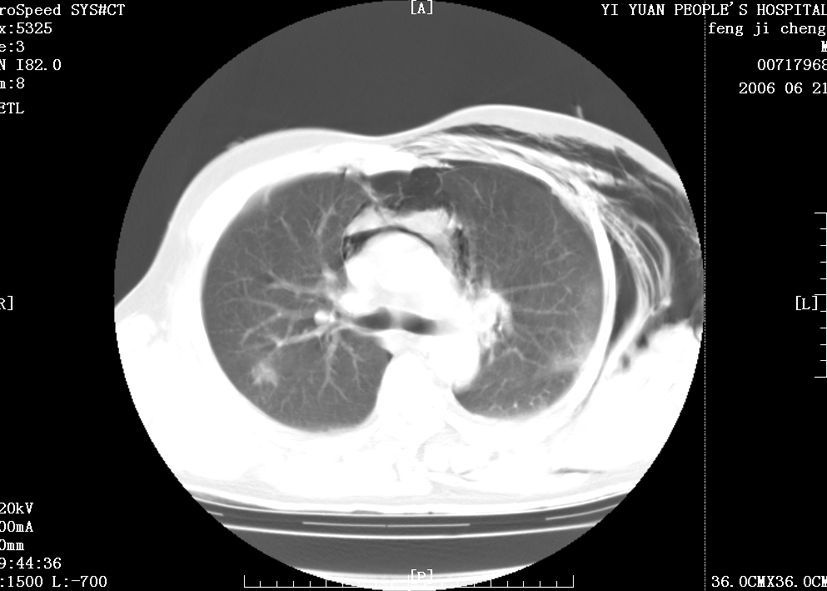
\includegraphics[width=.7\textwidth,height=\textheight,keepaspectratio]{./images/Image00223.jpg}
 \captionsetup{justification=centering}
 \caption{左侧胸部皮下气肿、纵隔气肿\\{\small 前纵隔内有许多不规则气体积聚区;左侧肋骨骨折、两肺挫伤}}
 \label{fig9-32}
  \end{figure} 

2.骨骼损伤:①肋骨骨折:胸部钝伤中的发生率约56%,CT还可显示气胸、血胸、肺挫裂伤等并发症;②胸骨骨折:相对少见;③胸锁关节脱位:CT易于显示,并可显示由其造成的对邻近器官的压迫和损伤。有时正常胸锁关节内亦有气体,勿误诊。

\subsection{纵隔内器损伤}

1.胸主动脉其大分支血管损伤:胸主动脉损伤以狭部多见。胸主动脉撕裂可见以下CT表现。①假性动脉瘤:紧贴主动脉的高密度或等密度圆形、椭圆形或不规则形影,胸主动脉可受压变形。增强扫描呈“晚进晚出”表现,瘤壁可强化,血栓不强化。②血管边缘不规则,壁厚薄不均。③夹层分离:即呈主动脉夹层表现。④主动脉周围血肿:很常见,紧贴主动脉者高度提示主动脉撕裂,远离主动脉者多为纵隔内小血管破裂所致。无明显强化。⑤伴发邻近器官的受压移位,胸骨、胸椎及第1~3肋骨骨折。

2.心脏及心包损伤:①心脏破裂者CT平扫见高密度心包积血及胸腔积血。②心包破裂者常致心脏向左后侧旋转,心脏突出于心包之外。有时有少量心包积气,有助于心包破裂的诊断。

3.气管和支气管损伤:80%以上的损伤分布在隆突周围2.5cm处。①常见的影像学表现是空气持续性进入纵隔和胸壁软组织内。②支气管外过度膨胀的气囊,有时可能是支气管损伤的早期征象。③在周围气体衬托下可直接显示气管、支气管的破口或断裂的部位及形态。④支气管撕裂伤可表现为同侧气胸和肺萎缩。⑤约10%病人伤后无异常表现。⑥可有气管狭窄、气管食管瘘、气胸、纵隔炎或支扩等并发症。

4.食管破裂:多由穿通伤引起,钝伤少见。可见继发的纵隔炎表现及纵隔积气和软组织肿胀。

5.胸导管损伤:极少见,常见原因是手术损伤。以持续性胸腔积液为主要表现,CT检查意义不大。

6.膈损伤:左膈是右膈的3倍。膈破裂CT表现为膈不连续,还可见腹腔内实体脏器或网膜疝入胸腔。

\subsection{肺挫伤}

肺挫伤是最常见的原发性肺损伤,在严重胸部钝伤的病人中占17%~70%。

\textbf{【病理机制】}
外力直接由胸壁传至其下方的肺,产生肺间质及肺泡的损伤。小血管破裂和肺泡毛细血管膜的破坏所致的出血在伤后1~24h进入肺泡及肺间质,并发生间质水肿。肺挫伤导致通气-灌注失调、肺内分流、肺顺应性减低、肺内水分增加。严重的可发生呼吸衰竭。

\textbf{【临床表现】}
胸痛、吸气性呼吸困难为主,部分有咳嗽、咯血或痰中带血。

\textbf{【CT表现】}
肺纹理增多、增粗,边缘模糊,伴单侧或双侧斑片状、大片状或弥漫性的肺泡实变,边缘模糊,以周围性局限性分布为主(图\ref{fig9-33})。支气管充气征难以见到,是因为血液填充邻近的小气道。国外有学者报道肺挫伤时胸膜下肺组织清晰,而其他疾病如肺膨胀不全或感染等其胸膜下组织混浊。挫伤往往在48~72h内就开始消散,完全吸收在伤后10~14天。但感染和呼吸窘迫综合征在此期间不可能完全消失。如伤后3天无吸收反而加重者则考虑有继续出血、继发感染等合并症。

\begin{figure}[!htbp]
 \centering
 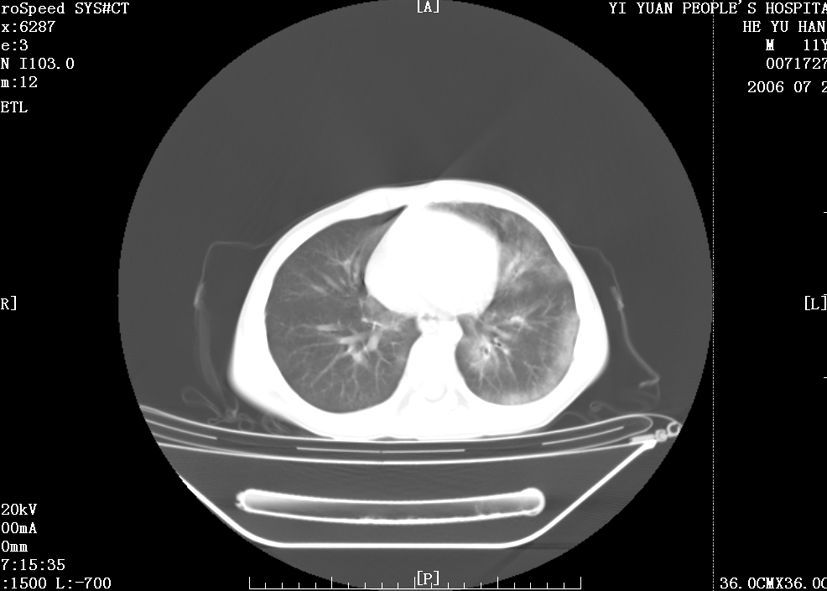
\includegraphics[width=.7\textwidth,height=\textheight,keepaspectratio]{./images/Image00224.jpg}
 \captionsetup{justification=centering}
 \caption{肺挫伤\\{\small 显示两肺有许多磨玻璃样高密度区,左侧显著}}
 \label{fig9-33}
  \end{figure} 

\subsection{肺撕裂伤}

肺撕裂伤周围常有肺挫伤,撕裂伤和挫伤在胸片上难以区分,CT则可区分。

\textbf{【病理机制】}
①气浪通过固定的不同肺组织界面而产生的剪切伤;②由于肋骨骨折而直接引起的肺撕裂伤;③在肺实质与胸膜紧密连接处的胸壁猛烈运动而引起的肺撕裂伤;④支气管受压,管腔内高压致远端肺泡破裂;⑤后部肺实质受压或推挤碰到椎体或肋骨所致。由于肺弹性回缩的结果撕裂往往是椭圆形的。

\textbf{【临床表现】} 与撕裂伤相近,表现为胸痛、呼吸困难、咳嗽、咳血等。

\textbf{【CT表现】}
肺组织撕裂,气体或血液溢入肺组织的裂口内,表现为创伤性肺气囊肿、气液囊肿或肺内血肿。①肺气囊肿和气液囊肿:表现为圆形、卵圆形或半圆形透亮囊腔或气液囊腔(图\ref{fig9-34})。②肺血肿:呈边缘清楚、密度较高的圆形、椭圆形或梭形分叶状影。但同时有肺萎缩或不张时则需肺复张后得以显示。③创伤性肺气囊可逐渐膨胀形成巨大的无通气功能的死腔。④肺血肿吸收较慢,通常于数日至数周内逐渐吸收缩小,完全消退可长达半年甚至1年,并可留有少许线条状瘢痕。

\begin{figure}[!htbp]
 \centering
 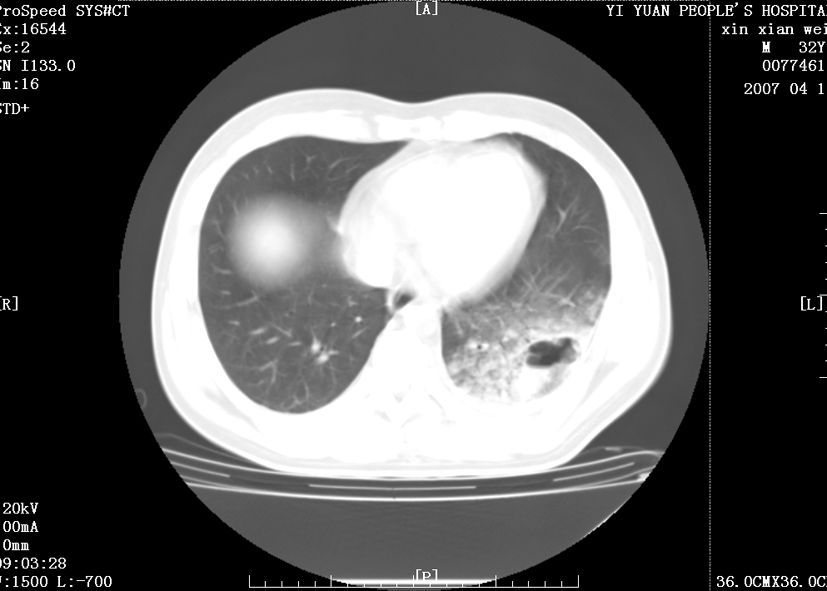
\includegraphics[width=.7\textwidth,height=\textheight,keepaspectratio]{./images/Image00225.jpg}
 \captionsetup{justification=centering}
 \caption{肺撕裂伤\\{\small 肺挫伤合并肺撕裂伤,示左肺底有大片状高密度灶,其内有欠规则撕裂含气腔隙}}
 \label{fig9-34}
  \end{figure} 

此外,肺挫伤和肺撕裂伤均可合并皮下气肿和纵隔气肿、外伤性膈疝、胸腔积液,以及纵隔、腹部脏器的损伤。

\subsection{外伤后肺不张和肺扭转}

\subsubsection{外伤后肺不张}

可能以肺挫伤或挫裂伤后气管内血块或因痰液引流不畅所致的痰液阻塞多见。此外,支气管创伤或断裂所导致的血液渗出和狭窄亦是不张的原因之一。

\subsubsection{肺扭转}

极其罕见,也极难诊断。即围绕肺门的肺组织发生轴向扭转。在成人多为肺叶或肺段切除后所致,在小儿可为胸部创伤的直接后果。在CT图像上,其诊断有赖于认识肺血管和叶、裂的错位;另一方面也可发展为缺血性梗死。如有老片比较,注意到原有病灶如钙化、肉芽肿发生的位置改变,有助于诊断。

\subsection{肺脂肪栓塞综合征}

本病是以急性呼吸功能紊乱为特征的、伴有脑部或全身症状的临床综合病征,常发生于严重创伤的病人(多发生于骨折后2~4天)。

\textbf{【病理机制】}
有以下几种学说。①微血管栓塞学说。肺毛细血管床广泛性脂肪栓塞导致急性肺心病和心衰。这种情况虽属可能,但极其罕见,不能解释所有的临床症状和影像学表现。②化学毒素学说:脂肪水解后产生脂肪酸,直接作用并损害毛细血管壁,引起肺出血、水肿和小叶性肺不张。③血小板凝集学说:血小板和红细胞凝集,引起组织胺和其他因子释放造成毛细血管壁的间接损害和血管内凝血。

\textbf{【临床表现】}
临床诊断的主要指标有:①皮肤和黏膜出血点;②非胸部创伤的呼吸功能紊乱;③非颅脑创伤的神经症状。

\textbf{【影像学表现】}
两肺散在的片状、磨玻璃状高密度灶,以中下肺中外带分布较多。病情进展,病变密集分布并融合成大片状影,呈典型暴风雪样改变。病变累及双侧,肺尖稀少或无病灶。一般胸膜、膈肌、心脏和大血管很少受累。

\subsection{刺激性气体引起的肺部损伤}

刺激性气体对人体的损害与气体的种类、浓度以及接触时间长短有关。发生作用的迟早则与气体的溶解度有一定关系。

\textbf{【病理】}
大多数刺激性气体(如氯气、二氧化硫、二氧化氮、有机氟、氨气)接触呼吸道黏膜后发生腐蚀作用,使黏膜充血、肿胀,进而坏死、脱落,肺间质水肿、小叶间隔肿胀增厚。严重者使毛细血管通透性增加,可导致肺泡性肺水肿。

\textbf{【临床表现】}
在接触刺激性气体后,可有咽喉部烧灼感,以及呛咳、流涕、流泪、气促、胸闷、呼吸不畅、头晕、恶心、昏厥等,以后可有一症状缓解期。经2~8h(长者12~48h)后症状可突然加重,严重者可有咯血或坏死物咳出、紫绀、血压下降,以致呼吸衰竭。继发感染有发热及呼吸道症状加重。

\textbf{【影像学表现】}
早期近肺门和两肺上部肺纹理增粗、模糊,从较淡的小斑片状影到较多的斑片状高密度灶,支气管壁水肿增厚。肺部病变的出现大多在24h内,表现为肺门周围及两肺中上部大片状浓密阴影(即肺水肿样改变)。如支气管阻塞可产生肺不张。如有坏死性支气管炎或剧咳可产生间质性肺气肿、纵隔及皮下积气或发生气胸,偶有胸腔积液。大量或长期地吸入刺激性气体可引起慢支,并发展为支扩,甚至发生间质纤维化。

\subsection{药物引起的肺损伤}

能引起肺部损伤的药物很多,主要有抗肿瘤药物、抗生素、抗代谢药物、抗惊厥药、镇痛药及抗心率失常药等。

\textbf{【病理】}
药物引起的肺部损伤的病理机制为过敏反应。其病理改变有:过敏性肺炎、非心源性肺水肿、慢性肺泡炎、肺纤维化、闭塞性细支气管炎并机化性肺炎(BOOP)、肺肾综合征、肺组织内药物沉着。有些药物可引起多种病理反应,少数可引起胸部淋巴结增大和胸水。

\textbf{【临床表现】}
急性过敏反应者用药即刻或短时间内出现咳嗽、气急,甚至休克。多为缓慢起病,有干咳、气急、不适、发热,有些伴有血中嗜酸粒细胞增高。肺肾综合征者有咳血和血尿。肺功能检查多为限制性通气障碍。

\textbf{【CT表现】}
①非心源性肺水肿:可伴胸水;②过敏性肺炎:早期呈外周性分布的多发斑片状实变和小结节,如不能吸收,后期可有弥漫性网状影,常有胸水;③慢性肺炎或肺纤维化:可伴有胸水、胸膜增厚;④BOOP;⑤肺肾综合征:呈网状影或小灶性实变影,后者可融合成片;可伴胸水;⑥肺部高密度灶:如乙胺碘呋酮在肺部沉着形成高密度灶;⑦淋巴结增大。

各种不同的药物各有其特点。①硝苯呋喃妥英:急性反应见于间断用药,血液中常有嗜酸粒细胞升高;影像学表现为两肺斑片状影,常伴少量胸水,甚似肺水肿,停药后24~48h恢复正常。慢性反应见于长期用药,表现为两肺广泛间质纤维化,常需激素治疗。②甲氨蝶呤:发生肺炎和间质性肺浸润,可有淋巴结增大。③马利兰、环磷酰胺、博莱霉素和争光霉素:肺部出现间质性纤维化。④硫唑嘌呤、青霉素、磺胺、四环素、苯妥英纳和甲基多巴:可引起肺泡炎。⑤二苯基海因(抗惊厥药):可引起纵隔或肺门淋巴结增大。⑥水杨酸盐类药物:是肺水肿和肺出血的公认原因。⑦乙胺碘呋酮:可引起肺内高密度灶,并可伴有楔形实变和局限性肺不张,邻近胸膜增厚。也可形成周围肺野肿块,甚至心肌密度增高。

\subsection{放射性肺损伤}

本病常由于胸部放射治疗所致。

\textbf{【病理】}
放射线的物理刺激,肺泡是主要损伤部位,基本病变为肺充血、水肿、肺间质增厚及肺泡腔萎缩变小。后期肺损伤以肺泡间隔的进行性纤维化为特征。“放射性肺炎”多发生在放疗后1~3个月,少数在1个月内。慢性纤维化一般发生在放疗后4~6个月(也有文献认为9个月或更晚),12~16个月时趋于稳定。美国放射肿瘤治疗协作组将发生在放射治疗开始后90天之内的肺损伤称为急性放射性损伤,发生在90天以后者称为后期放射性损伤。还有文献将其分为3期。①急性炎症期:照后1个月内,肺泡腔内可见渗出液和出血,支气管上皮细胞坏死脱落;②增生期:照后1~3个月,支气管和血管周围可见以淋巴细胞为主的炎性细胞浸润;③纤维化期:照后6个月,成纤维细胞增生和肺组织局造性实变。

\textbf{【临床表现】}
在放疗开始后,可在疗程中发生,但常见于放疗结束后。临床上有咳嗽、痰量少、白色泡沫样,有低热。严重者有明显气促、端坐呼吸及紫绀,甚至呼吸衰竭而死亡。慢性期广泛纤维化可导致肺不张、支扩,以及肺心病。

\textbf{【CT表现】}
早期表现为照射区稍高密度灶,边缘平直;还可表现为照射野内多发的斑片状高密度灶,边缘模糊;少数病灶超过放射野可能为患者对放射线的过敏反应所致(图\ref{fig9-35}A)。上述表现是可逆的。好转者病变范围逐渐缩小,密度逐渐降低或完全吸收。若病变未及时控制,可发展为慢性放射性肺炎(放射性肺纤维化),表现为放射野内散在斑片状实变区,夹有带状和条索状更高密度灶,肺体积缩小(图\ref{fig9-35}B)。进一步发展,肺纤维化加剧,肺呈密实的实变区,内有支扩,伴纵隔向患侧移位。有时可见纵隔增宽并可与肺部病变相融合,可称为放射性纵隔炎,常伴有胸膜肥厚粘连及积液。晚期可有肺动脉高压、肺心病。如大量纤维化后再出现渗出改变,则为继发感染的征象。如发现肿块区又有增大,且边缘较光整,则是肿瘤复发的征象,可伴有心包积液,且有时在放疗后几年发生。

\begin{figure}[!htbp]
 \centering
 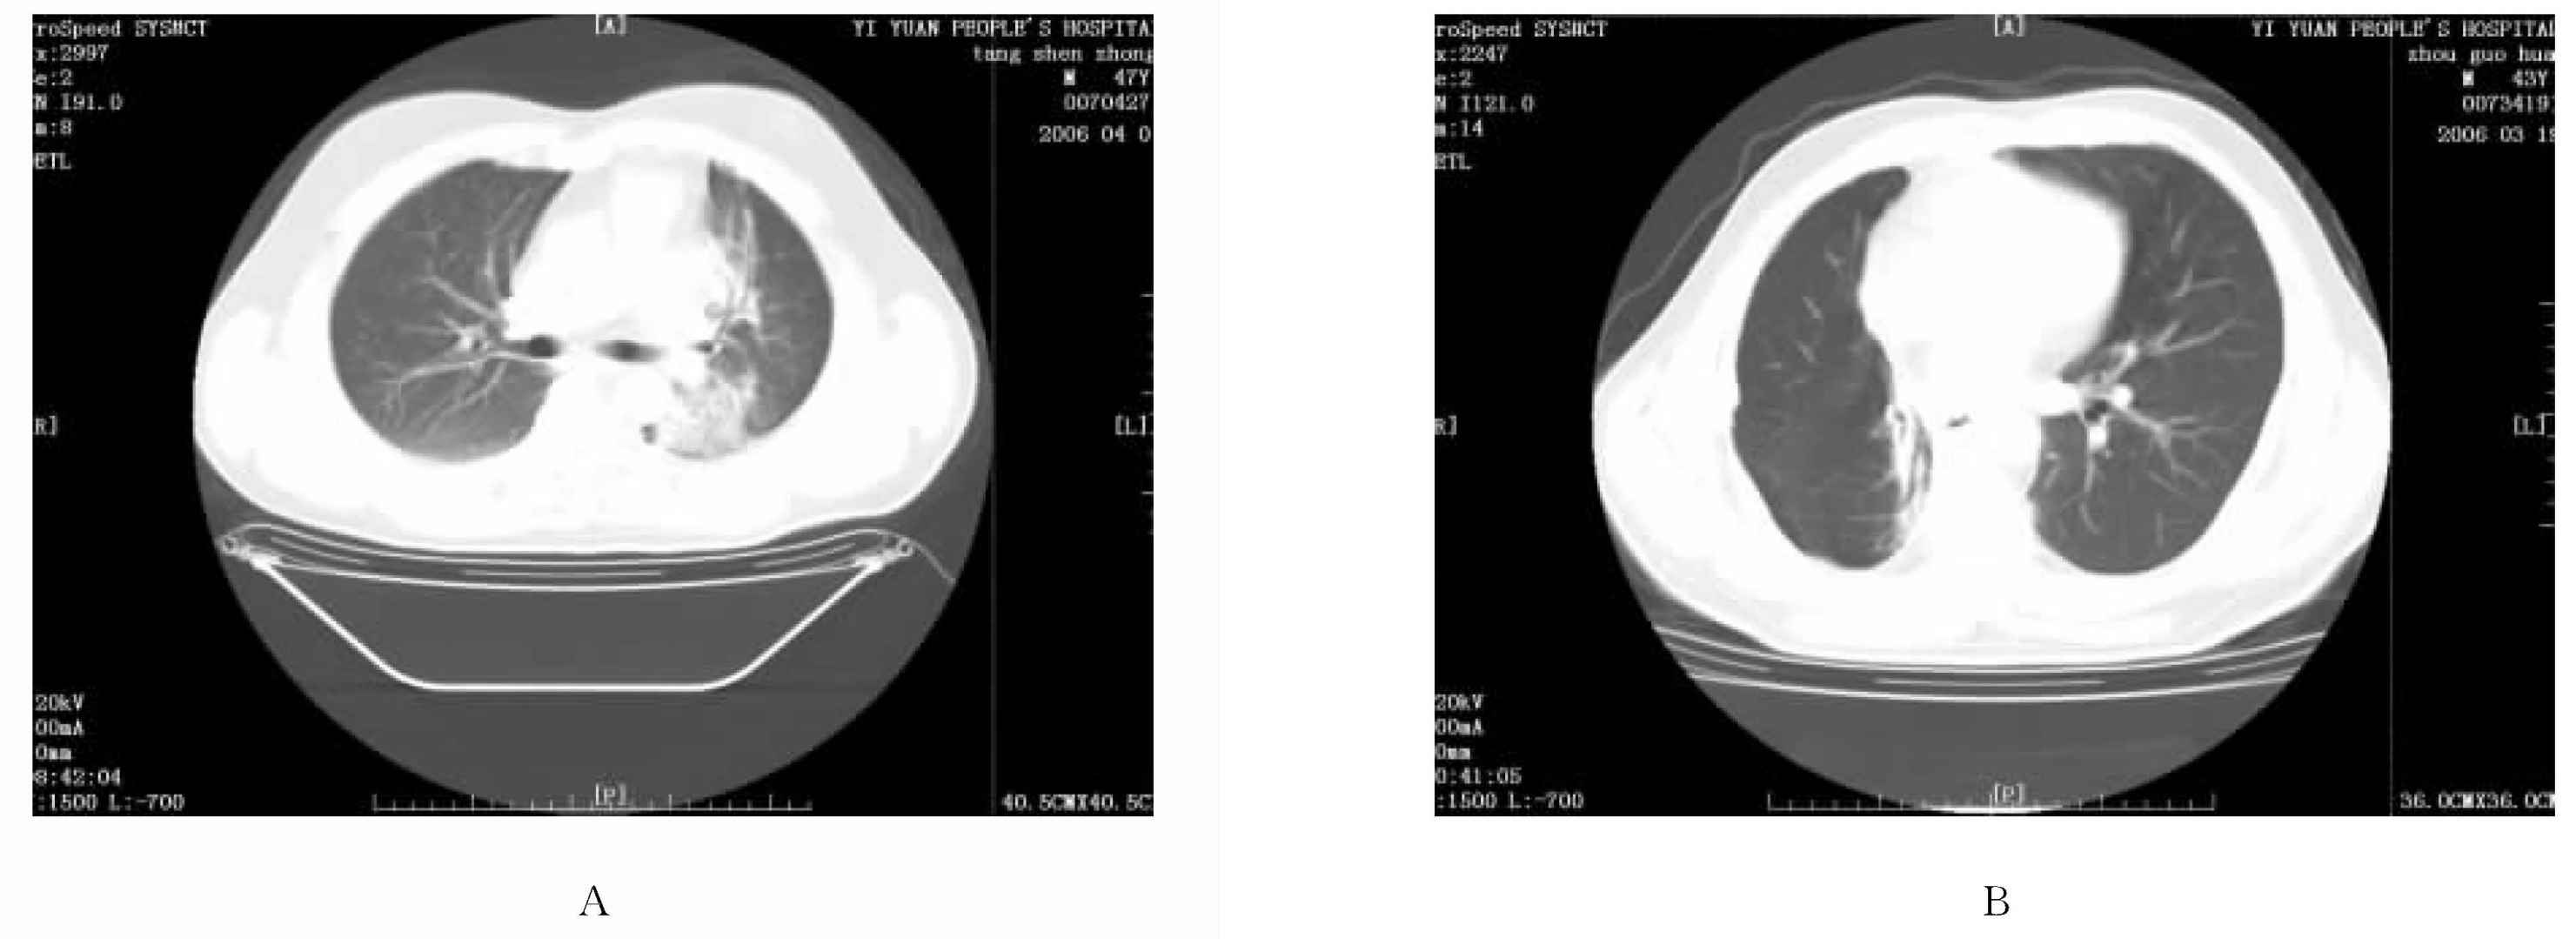
\includegraphics[width=.7\textwidth,height=\textheight,keepaspectratio]{./images/Image00226.jpg}
 \captionsetup{justification=centering}
 \caption{放射性肺损伤\\{\small A.左侧急性期损伤,照射区稍高密度灶,边缘模糊、平直;B.右侧慢性期损伤,照射区条索状更高密度灶,边缘清晰、平直}}
 \label{fig9-35}
  \end{figure} 

\section{尘肺}

\subsection{尘肺的分类}

尘肺是重要的职业性肺病,其种类很多,可概括的分为无机粉尘和有机粉尘两大类。其中以无机粉尘为多,而且最为重要。

1.无机尘肺:①矽肺:为长期吸入游离二氧化硅所致;②炭尘肺:为长期吸入煤炭、炭黑和石墨等粉尘所致,如煤尘肺、炭黑尘肺、石墨尘肺、活性炭尘肺等;③硅(矽)酸盐尘肺:为长期吸入结合状态的二氧化硅粉尘所致,如石棉肺、滑石尘肺、云母尘肺、水泥尘肺等;④混合性尘肺:为长期吸入含有游离二氧化硅和其他某些物质的混合性粉尘所致,如煤矽肺、铁矽肺等;⑤其他无机粉尘:如吸入铝及其氧化物所致的铝尘肺,或长期吸入电焊烟引起的电焊工尘肺等。

2.有机尘肺:①棉尘肺;②农民肺;③蔗尘肺;④茶尘肺。

\subsection{矽肺}

本病是由于长期吸入游离二氧化硅粉尘而引起的以肺组织纤维化为主的疾病,是尘肺中对人体危害最严重的一种。一般在持续吸入矽尘5~10年后发病,即使已停止接触亦可发病,即所谓迟发矽肺。

\textbf{【病理】}
其基本病理改变是慢性进行性肺间质纤维化和矽结节形成,矽结节是其特征性的病理改变。进入呼吸道的含矽尘粒只有直径10μm以下的能到达肺泡,其中2μm以下的多被吞噬细胞所吞噬。游离二氧化硅的化学作用在肺部的微小淋巴组织内引起增生性纤维改变,首先为纤维母细胞增生,其后产生胶原纤维和玻璃样变,进而形成小的初期矽结节,其直径一般在0.6mm左右。当矽尘粒继续在其周围产生纤维增生改变,矽结节可逐渐增大且可达2mm左右,往往多个矽结节融合,不断发展可融合成团状以至大块状纤维改变。此外,还可继发肺气肿和胸膜增厚粘连等改变。

肺结核是矽肺的重要合并症,其发病率在30%~60%之间。矽肺患严重肺结核的几率更高。其病理类型有两种:①结合型:矽肺结节与结核病变混合存在;②分离型:矽肺结节与结核病灶分离存在。

\textbf{【临床表现】}
在无合并症的情况下其发病和病程是缓慢的。由Ⅰ期发展到Ⅱ期,多为5~8年或更长。早期多无症状,因常伴气管和支气管炎而产生咳嗽。因肺气肿和细支气管痉挛而有呼吸困难、气急,最后导致心衰,还可伴有胸痛等症状,合并结核可有结核中毒症状。

\textbf{【CT表现】}

1.类圆形小结节:结节<1cm,一般为0.2~0.5cm大小,可发生钙化。结节位于小叶中心,弥散分布于两肺,以上肺及后部多见,尤以右上肺后部多见。与局部淋巴液流动慢,肺部清除尘粒能力相应减弱有关。矽肺结节的密度多高于血管,且常伴纤维化有助于与血管断面鉴别。一般>2mm者已成熟或比较成熟;而1~2mm者可能为成熟或不成熟的矽结节,也可由纤维索条的断面所构成,应注意分析。矽结节发展由少至多、由小至大、由淡至浓、由中下野向上野扩散。

2.进行性块状纤维化:一般均同时见有单纯的结节。块状纤维化多为类圆形、边界不规则,>1.0cm为三期矽肺的诊断依据(图\ref{fig9-36})。病变纵径(上下径)>2cm为融合,1cm说明开始融合,<1cm者不视为融合。矽肺团块常对称性位于中上肺野外带及锁骨下。块状纤维化钙化较常见,其中部分可见空洞。团块周围可有瘢痕性肺气肿。

\begin{figure}[!htbp]
 \centering
 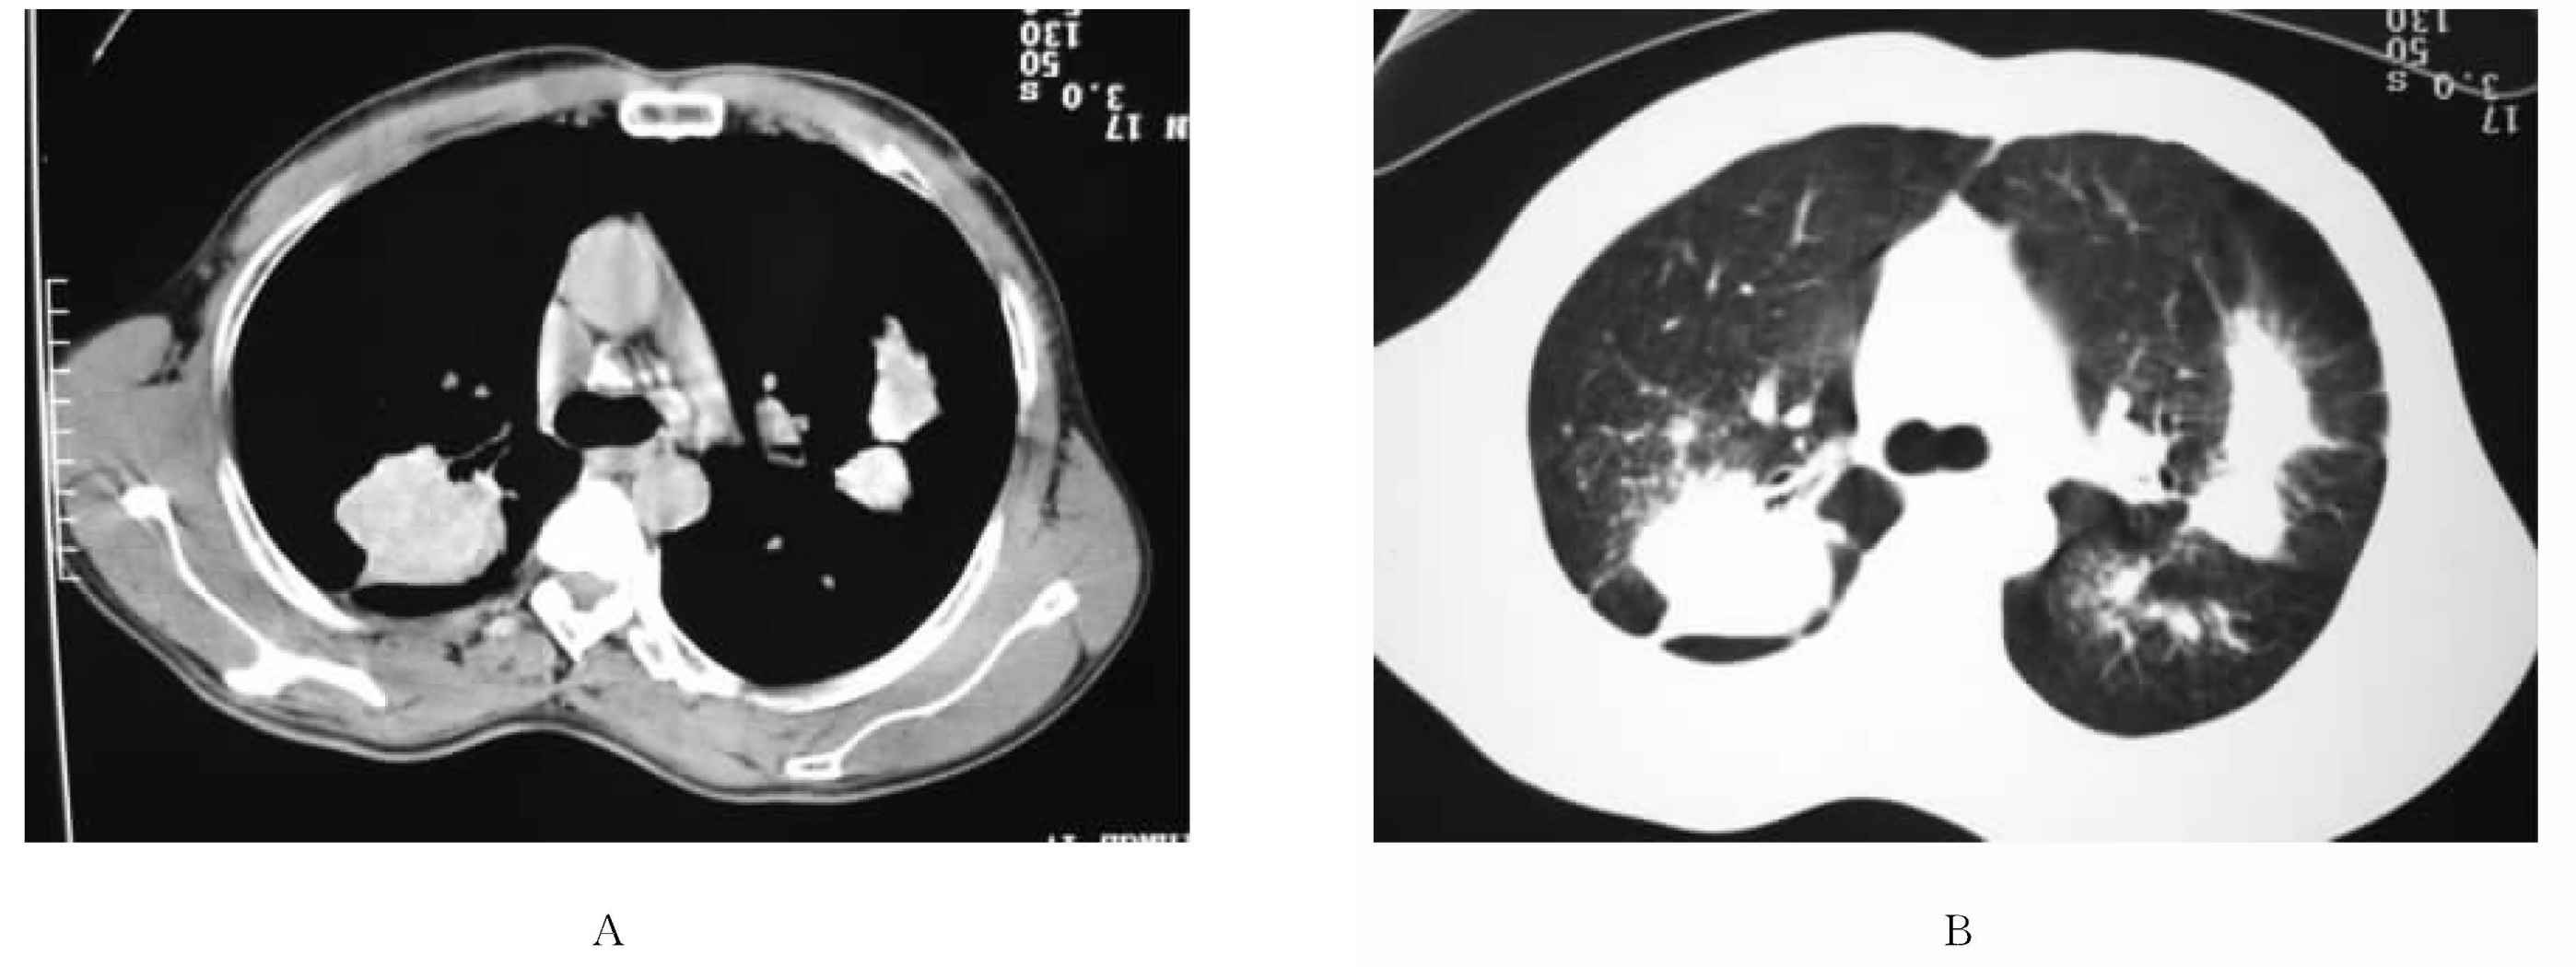
\includegraphics[width=.7\textwidth,height=\textheight,keepaspectratio]{./images/Image00227.jpg}
 \captionsetup{justification=centering}
 \caption{矽肺\\{\small 三期矽肺,两上肺有不规则块状纤维化,其内有钙化;气管隆突前、主肺动脉窗淋巴结有斑点状、弥漫性钙化}}
 \label{fig9-36}
  \end{figure} 

3.肺间质纤维化:表现为小叶间隔增厚、小叶内间质增厚、胸膜下弧形影及蜂窝状改变。

4.肺气肿:除瘢痕性肺气肿外,还可见小叶中心性肺气肿、全小叶肺气肿、小叶间隔旁肺气肿及肺大泡。

5.淋巴结钙化:一般在2cm以下,可见蛋壳状钙化、斑点状及弥漫性钙化。

6.胸膜增厚:可呈结节状及多发性胸膜增厚。

7.矽肺结核:①矽肺结核病灶形态多且不规则,边缘模糊,密度不均,多有空洞形成,病灶常位于两肺上野或分布不对称。②影像学表现变化迅速。总之,如果浸润性病灶局限于肺尖可考虑为结核。

\subsection{煤矽肺}

煤矿工人尘肺多属于煤矽肺,在单纯的煤尘肺和矽肺中,尤其前者少见。

\textbf{【病理】}
煤矽肺的基本病理改变属间质型。①间质纤维性变;②煤小灶:相当于矽肺的结节;③纤维团块:结节融合而成;④代偿性肺气肿。

\textbf{【临床表现】}
早期可无任何症状。当病变进展或合并感染可出现气短、胸痛、胸闷、咳嗽、咳痰等症状。晚期可引起肺通气功能减退。

\textbf{【CT表现】}
其特点是以广泛的索条状和网状纤维化为主,伴有散在的小结节。①间质纤维化改变:呈两肺广泛不规则条状影和网状影为间质纤维化表现,肺血管纹理扭曲、紊乱;HRCT有相应表现;②小结节阴影:比矽结节小,密度偏低,边缘不如矽结节锐利;③团块状纤维化:常在1~3年内成为典型的大块状融合,>4cm的团块常有坏死和空洞形成;④肺气肿:可为弥漫性或局限性,亦可出现肺大泡等;⑤胸膜肥厚粘连。

\subsection{Caplan综合征}

1953年Caplan指出,在同时患类风湿关节炎和尘肺的煤矿工人胸片上,可出现结节病灶。这种结节的结构与皮下类风湿结节相同而与尘肺引起的肺内结节迥然不同。这些结节仅在患类风湿性关节炎的患者中出现,甚为少见。

\textbf{【影像学表现】}
典型表现为有多个轮廓较为清楚的圆形结节,以两肺上部聚集较多,结节一般较大,直径可在0.5~5.0cm。这些结节易于产生坏死而形成空洞和钙化。空洞多发、壁薄,一般无气液平。

\subsection{石棉肺}

石棉是一种具有纤维结构的矿物,是镁、钙、钠、铁等与硅结合的硅酸盐。

\textbf{【病理】}
石棉肺的主要病理改变是肺部广泛纤维化及胸膜增厚,胸膜病变出现的早且较肺内改变显著。首先是细支气管周围产生水肿和肺泡内引起出血,随之在细支气管周围、小叶间隔内引起纤维化改变。与石棉肺有关的病变包括:①良性胸膜病变:胸膜斑、弥漫性胸膜肥厚、渗出及钙化等;②肺实质病变:肺石棉沉着症(由于吸入石棉而引起的肺实质纤维化)、圆形肺不张、良性纤维斑块、纤维索条等;③恶性病变:如胸膜间皮瘤、支气管肺癌。

\textbf{【临床表现】}
其临床表现主要为慢支、肺气肿、肺硬化及胸膜病变等症状,其中咳嗽、咳痰、气急和胸痛为主要症状,常伴有杵状指,可伴发其他疾病有相应的症状。

\textbf{【CT表现】}
①间质性纤维化改变:表现为广泛网格状影、小叶间隔增厚、胸膜下弧线影、磨玻璃样密度灶、肺内条索影等间质纤维化表现。②胸膜改变:主要为胸膜斑、胸膜弥漫增厚和胸膜钙化。胸膜局限性增厚厚度>3mm时,则称为胸膜斑。胸膜斑对石棉肺的诊断有重要意义。胸膜弥漫增厚较胸膜斑少见,其诊断标准为光滑连续的胸膜线影像至少超过1/4胸壁,伴或不伴肋膈角闭塞。胸膜增厚粘连以膈胸膜为主,晚期有胸膜钙化。③心包增厚粘连。④肺门改变:可增大、毛糙,淋巴结增大罕见。⑤可有弥漫性肺气肿表现。⑥局部胸膜明显增厚,形成软组织肿块时提示间皮瘤可能;若同时伴胸腔积液,则可能性更大。

\subsection{滑石肺}

滑石是主要由二氧化硅与镁结合的硅酸盐。

\textbf{【病理】}
它主要引起广泛肺间质纤维化,一般不形成结节,可有以下几种改变。①肺内异物性小肉芽肿:比较少见,大致是由于较纯粹的片状滑石尘所引起,一般不变成纤维化。②弥漫性间质性肺纤维化:与石棉肺一样也是从呼吸性细支气管周围开始,随后多伴有肺气肿。③不甚清楚的矽结节形成:是由于低浓度的游离二氧化硅所致。④胸膜斑。

\textbf{【临床表现】}
其临床症状较石棉肺轻。一般在接触滑石尘15年左右才产生,主要是劳动时气急,咳嗽和咳痰。如果接触滑石尘浓度很高,严重的气急症状可在接触粉尘2~3年即可产生。

\textbf{【影像学表现】}
较广泛的肺间质纤维化表现。肺门淋巴结增大,但不钙化。胸膜增厚粘连明显,有时可见条状或片状胸膜斑。如粉尘中含有一定浓度的游离二氧化硅,则可在中下肺出现散在的、约2mm左右的结节。极少形成纤维融合块。

\subsection{锡末沉着症}

\subsubsection{铁末沉着症}

常见于电焊工人。主要病理改变为二氧化铁沉积于肺间质所造成。

\textbf{【CT表现】}
广泛的、两肺散在的小结节,密度较矽肺低,或表现为部位不定的、不伴有纤维化的广泛磨玻璃样密度影。其结节开始为1mm左右,很少超过3mm,无融合征象,类似粟粒性肺结核。无肺门异常改变。脱离铁尘环境后上述表现可部分或全部消失。

\subsubsection{锡末沉着症}

本病是由于吸入二氧化锡的尘烟所引起。

\textbf{【CT表现】}
本病特点是尽管出现布满全肺的金属样致密影,但临床一般无自觉症状和阳性体征。一般无肺纤维化和肺门异常改变。

\subsection{棉尘肺}

本病不仅见于棉纺织工人,也可见于亚麻、大麻和黄麻等纺织工人。多发生在初步处理棉、麻等原料的清梳车间作业人员,而粗纺、细纺、织布车间的作业人员很少发生。

\textbf{【病理】}
棉尘中的组织胺或一种类似组织胺的物质,是引起棉尘肺患者支气管痉挛的主要因素。主要为慢性支气管炎和中等程度的肺气肿,并无向矽肺那样的特殊性纤维结节。往往可以见到圆形或椭圆形体,与在石棉肺中所见的长形石棉体类似。

\textbf{【临床表现】}
临床产生胸闷、气急和咳嗽,常反复发作。在每周休息日后上班时出现,其后逐日减轻至消失,再下一次休息日后出现症状,如此反复。

\textbf{【影像学检查】}
可无异常表现。严重者多为慢性支气管炎、肺气肿,可有轻度间质纤维化改变,但无特异性,必须结合病史诊断。

\subsection{农民肺}

本病是由于吸入发霉干草或发霉蔬菜的粉尘后,在呼吸道远端,主要在肺泡内所引起的过敏性疾病。其病原可能是随粉尘带入的一些嗜热性放线菌属的孢子。

\textbf{【病理】}
早期为中性粒细胞、嗜酸粒细胞和单核细胞浸润,分布类似小叶性肺炎。其后有非干酪性肉芽肿形成,并伴有明显的间质性肺炎和小支气管炎。至晚期肉芽肿消退,间质肺炎持续存在,可产生小块状、弥漫性纤维化,甚至形成蜂窝状改变。

\textbf{【临床表现】}
急性者与有害粉尘接触6h左右即可发病,但更多的病人起病缓慢。可有发热、寒颤、乏力、咳嗽、气急、呼吸困难等症状,有时可有咳血。如果不断接触有害粉尘,晚期可出现严重呼吸功能障碍。

\textbf{【影像学表现】}
早期的肉芽肿样病变,显示为弥散的颗粒状或小结节状阴影,肺尖和肺底较少。其大小自1毫米至数毫米、密度一般不高、轮廓不甚清楚。有时可呈大片状阴影。慢性期主要为弥漫性间质纤维化改变,呈蜂窝状,并出现肺气肿。本病的诊断需密切结合病史。

\subsection{蔗尘肺}

本病是由于长期吸入甘蔗纤维粉尘所引起的一种过敏性疾病,也有人认为它是隐藏在甘蔗纤维中的真菌所致。

\textbf{【病理】}
由增生性纤维母细胞、巨噬细胞和淋巴细胞所组成的肉芽肿性间质性炎症,形成小结节状病变,并有不同程度的肺内纤维化。

\textbf{【临床表现】}
主要是气急,可有咳嗽、咳痰、胸痛、发热、寒颤和不适等症状,有时可有咳血。

\textbf{【影像学表现】}
急性期表现为两肺有弥漫性细小结节影,类似粟粒性肺结核,以两下肺较密集,可融合成片,肺门可增大。反复慢性发作形成网状、蜂窝状纤维化表现。

\section{肺结缔组织疾病}

\subsection{概述}

结缔组织疾病亦称为胶原血管性疾病,属自身免疫性疾病。

\subsubsection{病理改变}

主要包括结缔组织的黏液水肿、炎性坏死、类纤维蛋白变性和纤维增生。由于结缔组织广泛分布于全身各处,因此在疾病的不同时期可侵犯体内各种脏器如皮肤、关节、心脏、血管、肺、肾、脑等。

\subsubsection{常见疾病}

较常见的侵及肺部的结缔组织疾病包括系统性红斑狼疮(SLE)、多发性结节性动脉炎、Wegener肉芽肿、硬皮病、皮肌炎、类风湿性和风湿性肺病;还有干燥综合征、白塞(Behcet)氏病等;强直性脊柱炎、变应性肉芽肿性血管炎、复发性多发性软骨炎亦属结缔组织疾病,均属全身性自身免疫性疾病,均可有肺部以及骨关节病变出现。

\subsubsection{系统性血管炎}

又称为系统性坏死性血管炎。其特征是血管壁的炎症和坏死,这一名称代表临床上一大组与血管坏死性炎症过程有关的综合征,这比过去流行的命名如坏死性动脉炎和多动脉炎(包括多发结节性动脉炎和其他过敏性动脉炎)更可取。因为这些疾病不仅累及动脉和小动脉,也累及静脉和毛细血管。其影像学表现以肺改变为主,骨关节改变较少见(表现较轻,主要是关节肿胀,无特征性)。

这类血管炎主要包括:①多发性结节性动脉炎;②变应性肉芽肿性血管炎:与多发动脉炎相似;③超敏性血管炎:亦称白细胞裂解性血管炎,包括血清病、过敏性紫癜、冷球蛋白血症、低补体血症性血管炎、伴发于结缔组织病的血管炎、伴发于炎症状态的血管炎、伴发于恶性病变的血管炎;④Wegener肉芽肿病;⑤淋巴瘤样肉芽肿病:亦称多形性网织细胞增生症;⑥多发性大动脉炎:又称高安氏病、无脉症等;⑦中枢神经系统肉芽肿性血管炎;⑧皮肤黏膜淋巴结综合征:又称川崎病。

\subsubsection{影像学表现}

本组疾病主要表现为:①肺门增大;②肺间质改变;③肺实质改变:病变反复发作,有的呈迁移性(即一处吸收而它处又出现,是红斑狼疮的一种征象);④肺结节和肿块:肺类风湿病、多发性结节性动脉炎、Wegener肉芽肿均可出现;⑤盘状肺不张(节段性肺不张);⑥胸膜增厚、粘连、胸腔积液:常与肺部病变并存,亦可单独出现;⑦心脏改变:多为心肌炎和心包积液所致,亦可有肺心病表现,心衰者可见肺水肿;⑧不同类型的结缔组织疾病可有胸外表现:如骨关节、消化道改变等。

其病理组织学和HRCT可表现为以下几种形式。①慢性间质性肺炎:最常见;②弥漫性肺泡损害:以两肺磨玻璃样影和实变影为主(图\ref{fig9-37}),伴慢性间质性肺炎及胸膜渗出,如SLE;③淋巴细胞性间质性肺炎;④闭塞性细支气管炎并机化性肺炎(BOOP);⑤肺出血;⑥肺动脉高压;⑦气道病变:多为闭塞性细支气管炎(BO)。

\begin{figure}[!htbp]
 \centering
 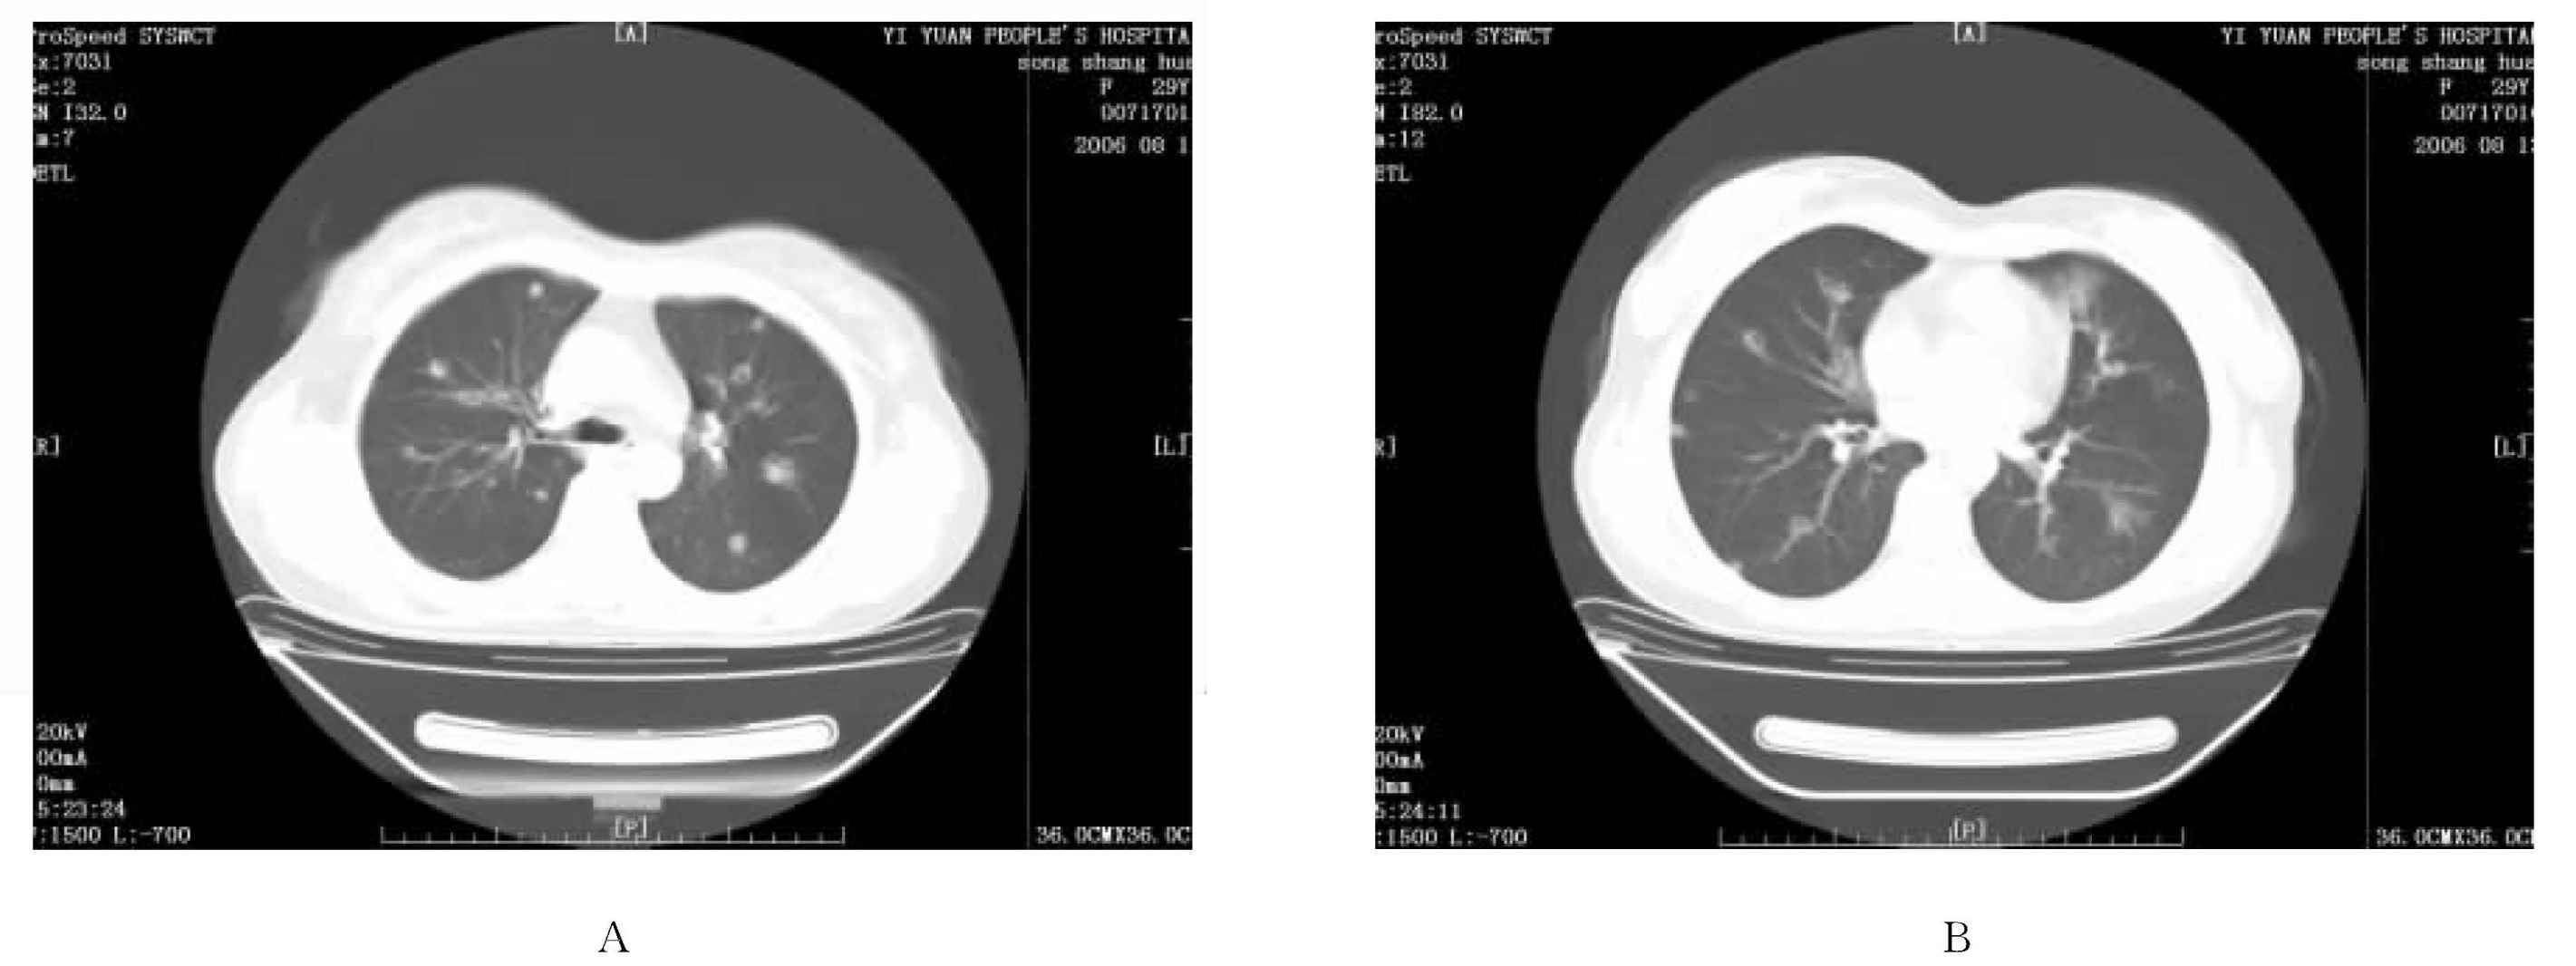
\includegraphics[width=.7\textwidth,height=\textheight,keepaspectratio]{./images/Image00228.jpg}
 \captionsetup{justification=centering}
 \caption{天疱疮并肺部病变\\{\small 两肺散在分布有许多高密度结节,部分结节其内有坏死;还可见少许磨玻璃样密度灶(本病例经肾上腺皮质激素治疗病灶吸收)}}
 \label{fig9-37}
  \end{figure} 

\subsection{系统性红斑狼疮}

本病以侵犯皮肤为主,但几乎侵犯全身任何脏器。除皮肤外,还较易侵犯心血管系统、肾脏、中枢神经系统、肺和浆膜(胸膜和心包膜)。

\textbf{【病理】}
病变局限在小动脉壁内,发生血管内皮炎,然后扩展到血管周围。在肺内可致肺充血、出血和炎性浸润,但较少形成广泛纤维化及蜂窝肺。胸膜病变通常为纤维蛋白性胸膜炎。

\textbf{【临床表现】}
好发于20~50岁的女性,男女之比为1∶10。常见两侧面颊呈对称性蝶翼状皮肤红斑,亦可见于躯干和四肢。全身症状有疲劳、乏力、厌食、发热和体重下降。95%有关节痛,78%有关节炎,亦可有淋巴结及肝脾增大等。侵犯肺部有干咳、气急、胸痛,甚至咯血。

\textbf{【CT表现】}
①斑片状、磨玻璃状或类结节状肺实变:以两肺底和外带多见,可见含气支气管征(图\ref{fig9-38})。可由肺炎出血(少见)、急性狼疮性肺炎或肺水肿(为肾损害尿毒症或心肌损害心衰所致)引起。②节段性肺不张:呈楔形、条带状高密度灶,有收缩表现,以肺底多见。③肺间质纤维化:HRCT见于近30%病人,蜂窝肺很少见。④胸膜改变:见于50%病人。胸腔积液是本病最常见的和早期的表现,为病变直接侵及胸膜或其肾病所致,多为两侧,通常为少量,亦可大量。⑤心脏增大和心包积液,后者常见。⑥肺内薄壁空洞形成,但极少见。

\begin{figure}[!htbp]
 \centering
 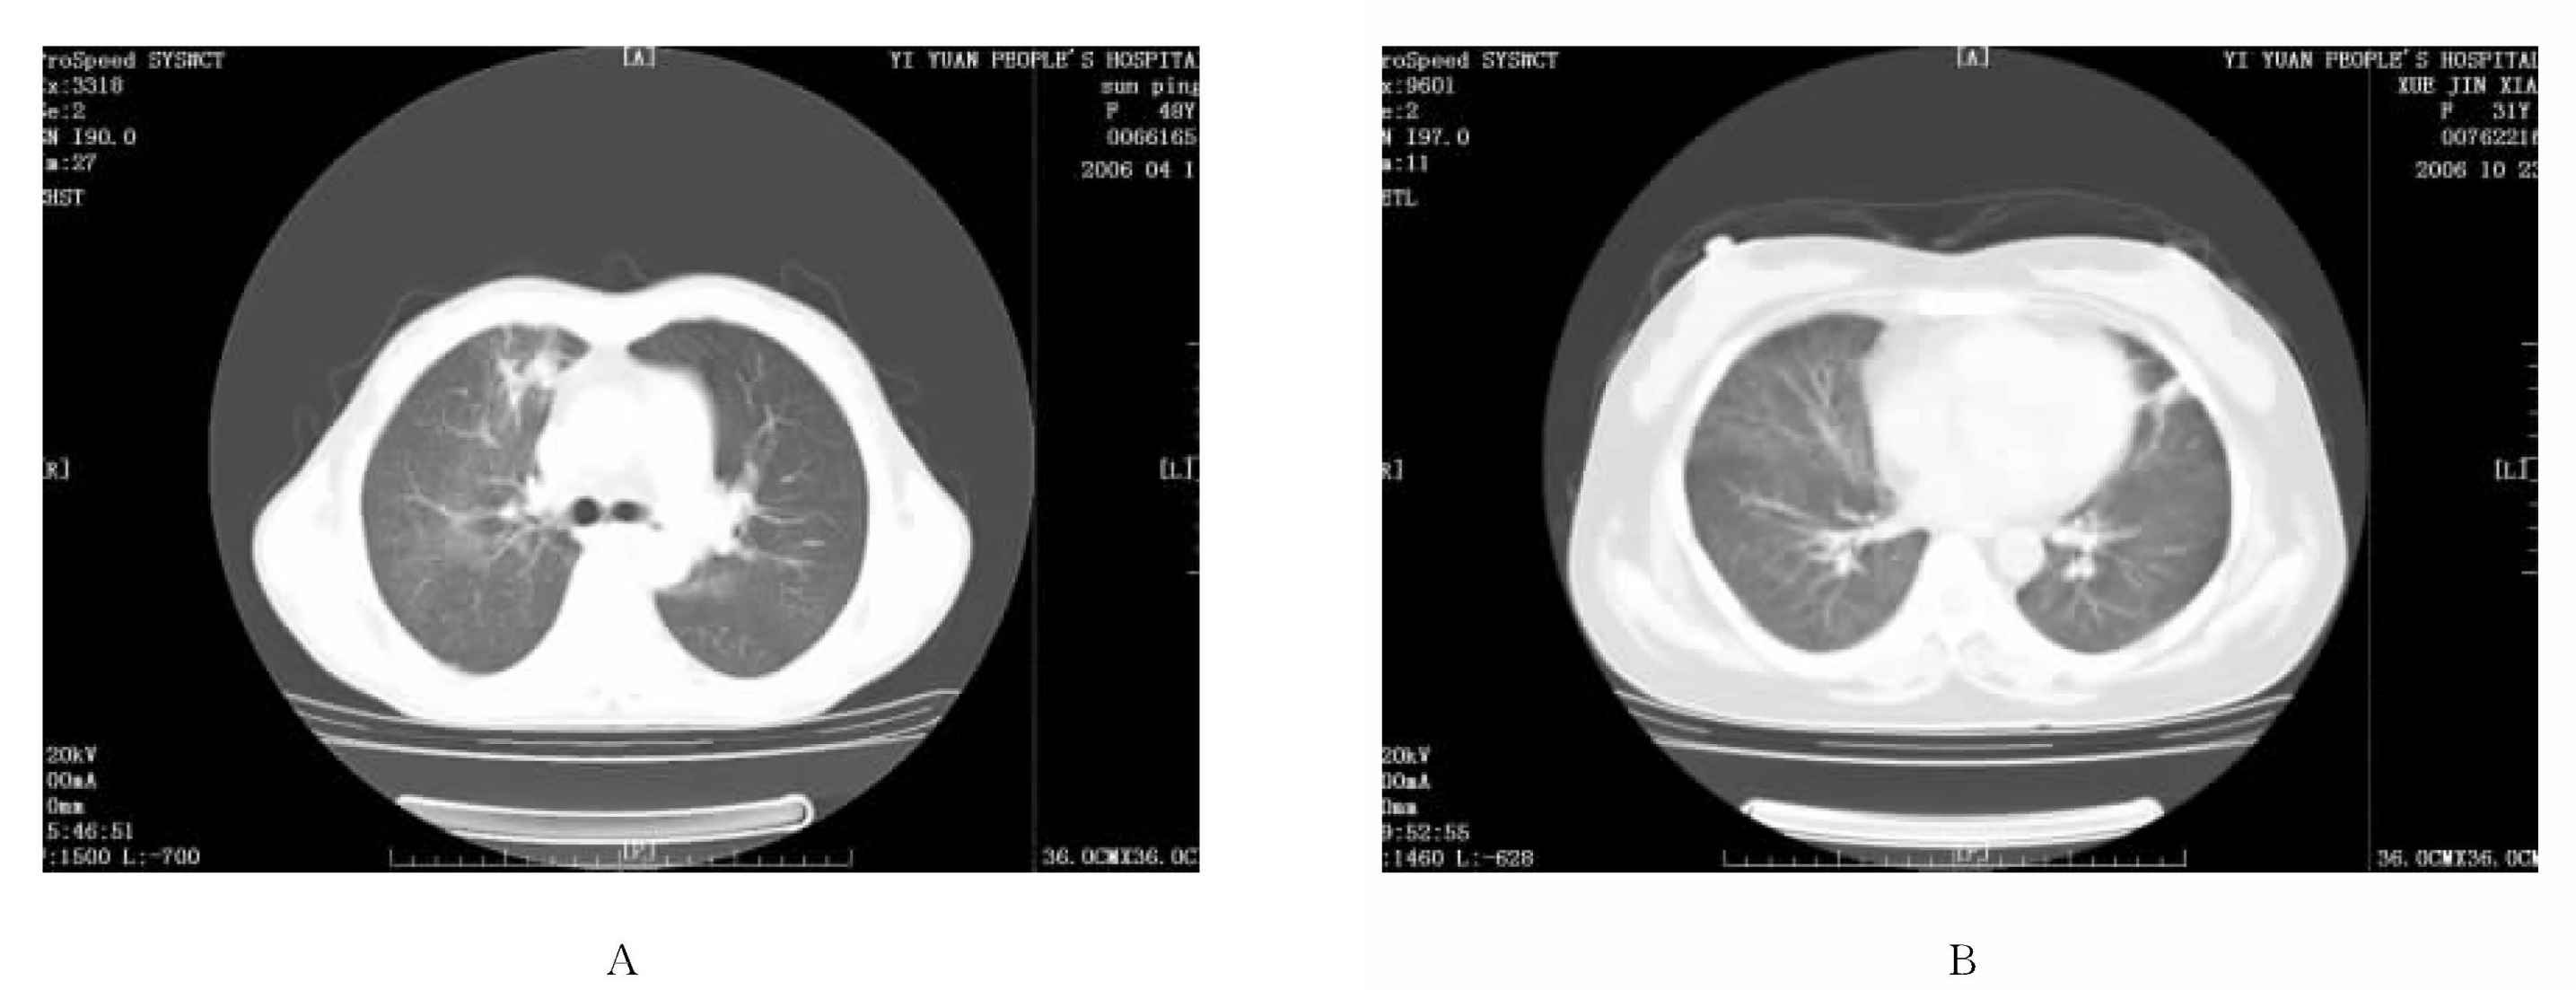
\includegraphics[width=.7\textwidth,height=\textheight,keepaspectratio]{./images/Image00229.jpg}
 \captionsetup{justification=centering}
 \caption{系统性红斑狼疮\\{\small A、B为同一患者,两肺以磨玻璃样病灶为主}}
 \label{fig9-38}
  \end{figure} 

\subsection{类风湿性肺病}

类风湿性关节炎与肺部病变的关系尚有争论,有的肺部病变出现在关节炎之前。虽然类风湿关节炎多见于女性,但关节外病变则以男性较多见。

\textbf{【病理】}
主要病理改变为肺间质纤维化、胸膜炎症和渐进坏死的肺结节。早期为非特殊性间质性肺炎,以水肿和细胞浸润为主。肺炎吸收后逐渐出现纤维化病变。胸腔积液是本病胸部最为多见的表现。肺的坏死结节与皮下类风湿结节完全相同,通常发生于重度类风湿关节炎或有多发皮下结节的患者,结节中心有类纤维蛋白变性和坏死。

\textbf{【临床表现】}
气急、咳嗽、胸痛和杵状指,可并发肺心病。有皮下结节者易并发肺间质性病变。胸腔积液可在关节炎之前出现。坏死性结节除长得很大或继发感染外,通常无症状。

\textbf{【CT表现】}
①广泛性肺间质纤维化:见于2%~9%的病人。HRCT呈外围性分布的网状影、不规则小叶间隔增厚和牵拉性支扩(图\ref{fig9-39})。随病变进展出现蜂窝肺和肺容积缩小,极少数纤维化局限于上叶并含空洞,类似肺结核。②胸膜病变:最常见。胸膜增厚较积液常见,积液常为单侧,可为包裹性,可伴心包炎。胸腔积液可数月数年不变,单侧较双侧多见,且多不伴肺内病变。③肺结节:少见。两肺有大小不等的多发性结节,大结节常散在分布,细小结节弥漫分布;结节偶为单发。结节轮廓清楚、光整,常位于肺的外围靠近胸膜处,结节亦可发生于胸膜和心包膜。结节直径为0.3~7cm,常出现厚壁空洞,内壁光滑。关节炎改善时,空洞变薄,并逐渐消失;当关节炎加重时空洞可以重新充填变为密实阴影。④气道疾病:多发生,如BO和BOOP。⑤Caplan综合征。

\begin{figure}[!htbp]
 \centering
 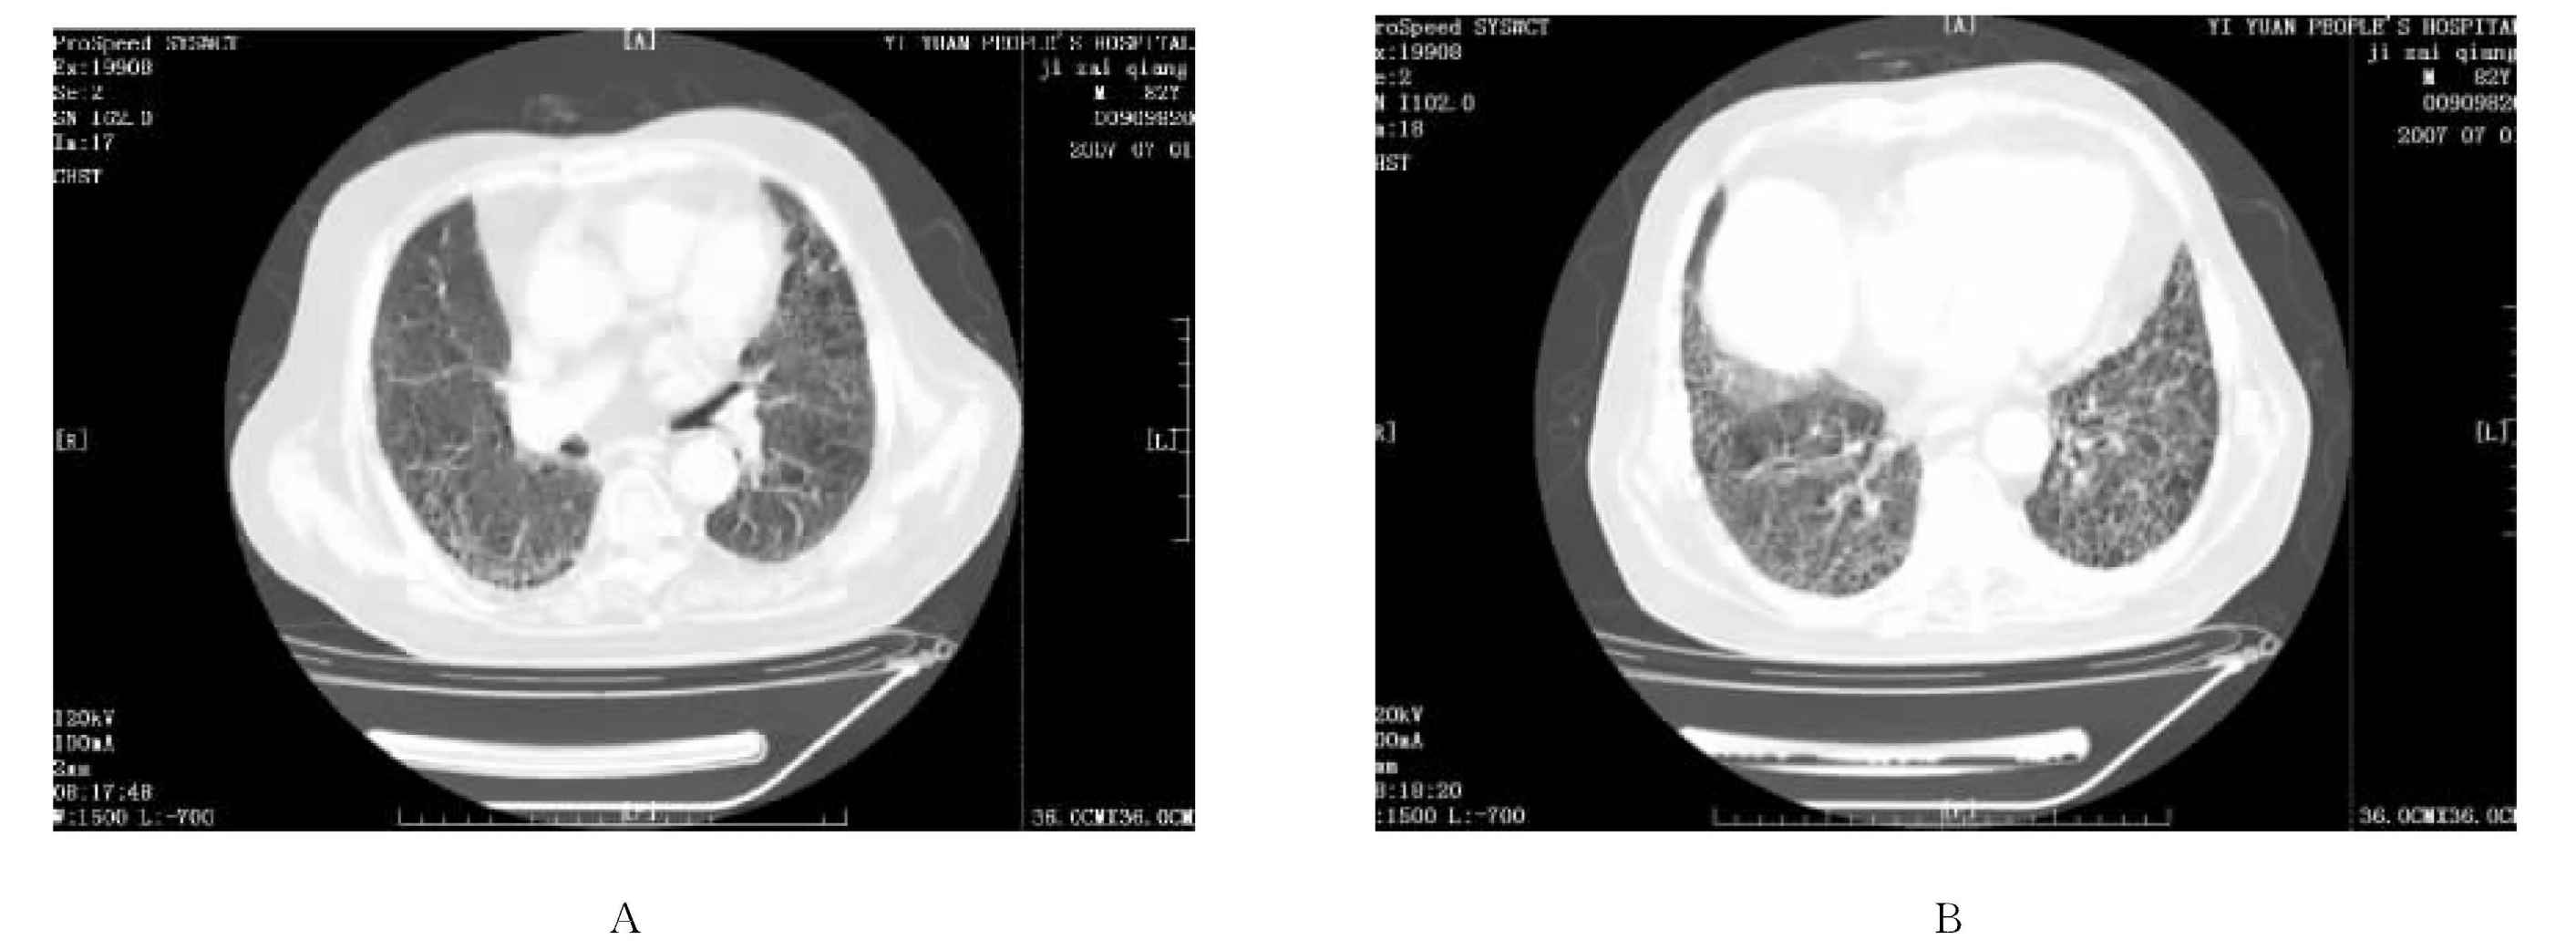
\includegraphics[width=.7\textwidth,height=\textheight,keepaspectratio]{./images/Image00230.jpg}
 \captionsetup{justification=centering}
 \caption{类风湿性肺病\\{\small A、B为同一患者,HRCT呈外围性分布的网状影、小叶间隔不规则增厚,以肺底显著}}
 \label{fig9-39}
  \end{figure} 

\subsection{硬皮病}

本病亦称为进行性系统性硬化。病因不明,病变主要侵及皮肤、肌肉、骨关节、胃肠道和心、肺。

\textbf{【病理】}
本病以胶原产生过剩为特征,导致肺、皮肤、脉管和内脏器官的纤维化。表现为结缔组织进行性的黏液水肿、硬化和萎缩,皮肤、肌肉、骨骼系统和多种内脏的小动脉阻塞性病变。肺部病变主要为广泛的肺间质纤维化,最后形成蜂窝状改变,常合并有血管炎和肺动脉高压。

\textbf{【临床表现】}
以30~50岁女性多见,男女之比为1∶3。皮肤改变是诊断本病的主要依据。病程分为浮肿期、发硬期和萎缩期。手足出现雷诺现象,2/3病人有肺部症状。最常见的症状是活动性呼吸困难、干燥、干咳,还可引起紫绀和肺功能减退,进而出现肺心病的表现。本病肺癌发生率增高。

\textbf{【CT表现】}
①肺广泛间质纤维化:为最常见的表现,约91%HRCT可发现病变。表现为磨玻璃样密度影、小叶间隔增厚等表现,随病变进展见长线影、网状影、蜂窝、牵引性支扩。病变亦多位于肺的外周和下叶。②1/3有胸膜增厚、粘连,还可见肺门血管增粗、心脏增大伴心包积液。③有时可见食管扩张,并可见吸入性肺炎。④60%有纵隔淋巴结增大。

此外,X线平片可见以下情况。①牙周膜增宽:正常为0.2~0.5mm,本病可增宽4倍,约60%的患者有此征象,对诊断有特征性意义。②指(趾)端、尺桡骨远端、锁骨端骨质吸收变短。③指端腹侧或关节周围软组织钙化,指端骨吸收见于多种疾病,但与软组织钙化并存者仅见于本病。④食管扩张、蠕动减弱、排空减慢、管腔狭窄。

\subsection{皮肌炎和多肌炎}

本病少见,属结缔组织边缘性疾病。

\textbf{【病理】}
特点为非化脓性多发性肌炎、皮肤炎和退行性变,并可侵及其他结缔组织和内脏。肺部主要病理改变为广泛间质纤维化、肺泡壁和肺微血管基底膜增厚。

\textbf{【临床表现】}
以女性多见,有儿童和中年两个发病年龄高峰。典型的多肌炎病人首发表现为躯干横纹肌进行性无力;皮肌炎病人除肌无力外还有皮肤改变。肌肉有压痛。呼吸系统有气急、声音嘶哑或音调改变,呼吸肌力减退严重者可产生呼吸困难和紫绀,还可有心脏症状。合并恶性肿瘤的几率较高,多见于乳腺、肺、和卵巢。

\textbf{【CT表现】}
肺间质纤维化约见于5%~30%的病人。表现为细网状影、磨玻璃状影,渐发展为粗网结节影和蜂窝,肺底部显著。气腔实变常由BOOP引起,可有少量胸腔积液。由于膈肌运动减弱可有节段性肺不张。如有咽肌麻痹可出现吸入性肺炎和节段性肺不张。心脏可慢性进行性普遍增大;也可因肺间质纤维化并发肺动脉高压和肺心病表现。

\subsection{干燥综合征}

\textbf{【病理】}
基本病理变化为泪腺、唾液腺因大量淋巴细胞浸润而引起纤维化和萎缩。5%~10%可累及腺体外。肺组织因各种炎性细胞浸润而广泛间质纤维化和肺动脉炎。

\textbf{【临床表现】}
多见于绝经期前后40~50岁的女性,男女之比为1∶9。以眼干、口干和多发游走性类风湿性关节炎(或其他结缔组织疾病)三大症状为特征。患者多反复发生呼吸道感染。

\textbf{【CT表现】}
①弥漫性间质纤维化:主要表现为磨玻璃影,支气管血管束和小叶间隔增厚、囊腔;②支气管炎和肺炎:反复发生,最后发生支扩;③肺不张:多为节段性肺不张;④胸腔积液和胸膜增厚;⑤假性淋巴瘤:表现为大小不等的结节病灶或片状影;亦可发展为淋巴瘤,出现纵隔淋巴结增大和肺肿块。

\subsection{风湿性肺炎}

本病少见,而且存在争议。有些学者从临床的发病情况、治疗反应和病理检查认为有风湿性肺炎存在,而有些学者则认为其病理不具特殊性,可能属于亚急性肺水肿。

\textbf{【临床表现】}
临床上病人有风湿和风心病,可为风湿性全心炎和风湿性瓣膜性心脏病的症状。

\textbf{【影像学表现】}
肺部炎症可为节段性或融合成大片的实变阴影,形如大叶性肺炎;也可显示为两肺的广泛实变;亦可形如肺水肿;少数呈粟粒样改变,这些均无特征性。本病胸膜改变多为干性胸膜炎。

如未患心衰、肺水肿的病人,肺部出现上述炎性改变,经抗生素治疗无明显疗效,而大量激素治疗效果显著时,可考虑为风湿性肺炎。

\subsection{强直性脊柱炎的肺部病变}

本病原因不明,主要累及躯干骨,男女之比为3∶1。国外有人统计,约1.2%患者胸片表现有上叶肺纤维化。

\textbf{【影像学表现】}
X线表现为肺尖部网状结节影,随病情进展病灶融合,常伴发肺尖大泡和空洞,类似肺结核。HRCT最常见的表现为肺周边部间质病变、支气管扩张、间隔旁肺气肿和肺尖纤维化。结合脊椎表现是诊断的有利证据。

\subsection{多发性结节性动脉炎}

本病是全身广泛性小动脉壁的炎性病变,它也是一种过敏性血管炎,可侵犯小静脉。

\textbf{【临床表现】}
其临床症状复杂多变,以支气管哮喘、嗜酸粒细胞增多和周围神经炎“临床三症”为主要表现。

\textbf{【影像学表现】}
①弥漫性肺间质病变:支气管血管束增粗毛糙,自肺门向外扩展,多见于中下肺,也可如蝶翼状。②肺实质和血管周围的浸润影:表现为两中、下肺有大小不一的结节状或片状、磨玻璃样影,密度均匀、边缘较清晰。浸润广泛者近似对称和非对称性肺水肿,称为“肺荨麻疹”。病变多为一过性,吸收快,也可由于梗死或坏死而形成空洞。③胸腔积液和心包积液:多为双侧,量少。

\subsection{变应性肉芽肿性血管炎}

本病为一种过敏性血管炎和肉芽肿性坏死性脉管炎,几乎均发生于哮喘病人。

\textbf{【临床表现】}
常见于30~50岁,无性别差异。病人典型表现为哮喘、嗜酸粒细胞增多、发热和过敏性关节炎。

\textbf{【CT表现】}
主要表现为斑片状、非节段性实变或磨玻璃影;实变可呈周边分布,但常为暂时性的。少见表现包括结节(结节空洞亦少见)、小叶间隔增厚和支气管壁增厚。此外,30%病人有胸腔积液。

\subsection{肺Wegener肉芽肿}

本病亦称为坏死性肉芽肿,是一全身性自体免疫性疾病,以上下呼吸道肉芽肿性脉管炎、肾小球肾炎和小血管脉管炎为特征。可多器官受累,肺最常见(约占94%)且病理变化最典型。

\textbf{【病理】}
以坏死性小血管(动、静脉)脉管炎和结节状凝固性坏死肉芽肿为病理特征。坏死结节周围有大量成纤维细胞和瘢痕组织。

\textbf{【临床表现】}
本病半数以上发病于30~50岁,男多于女。典型表现为上呼吸道病变、肺病变和肾小球肾炎三联征。胸部常见的症状有发热、咳嗽、咯痰和咯血。弥漫性肺出血和继发感染是常见并发症。实验室检查可有血清抗白细胞胞浆抗体升高、血清免疫球蛋白升高、贫血。

\textbf{【CT表现】}
①双肺大小不等的多发结节,结节大小从数毫米至9cm,为血管炎和肉芽肿形成的病灶。结节边缘光滑,形似转移瘤;也可因炎性改变而边缘模糊,且可有长毛刺;有时可见供养血管征和支气管气像。在病灶附近有时可见血管炎征象,即周围肺动脉直径大于并行的支气管直径或(和)形态不规则。②空洞形成,相当常见,出现于1/3~1/2的病例,可在1周内形成空洞。空洞开始壁厚,内壁不整,以后发展为薄壁空洞甚至形似囊肿。③大小不一、边缘模糊的片状浸润性病灶,病灶多局限于中、下肺,可有游走性。④常有胸腔积液;胸膜下结节可使胸膜楔形增厚;坏死灶破裂形成血气胸。⑤气管壁增厚、管腔狭窄。⑥肺门、纵隔或锁骨上淋巴结增大。⑦可有肺出血、肺水肿、支气管肺炎、肺梗死、肺不张、肺实质或间质纤维化及支扩表现。⑧鼻腔、鼻窦软组织肿块和骨质破坏。

总之,本病以病灶多样性(可为结节状、粟粒状、片絮状)、多发性、多变性(浸润病变短暂和游走)、空洞形成等为特征。结合病史可与转移瘤、脓毒性肺栓塞鉴别,但与其他肺血管炎伴肉芽肿的疾病如肺淋巴瘤样肉芽肿等难以鉴别。

\subsection{白塞(Behcet)病}

本病是以细小血管炎为病理基础的慢性进行性、复发性、多系统受侵的疾病。胸部损害比较少见,累及率为5%~10%。

\textbf{【病因病理】}
其病因不明,可能与病毒感染、自身免疫、遗传等因素有关。病理可表现为两种类型:即以肺血管病变为主或以肺间质病变为主,一般认为以前者较多见。全肺大小血管均可受累,表现为节段性血管炎,还有血栓形成、梗死及动脉瘤形成。这些血管病变中7%为动脉,25%为静脉,68%为动静脉受累。

\textbf{【临床表现】}
多见于20~40岁男性,男女之比约2∶1。临床诊断标准为:复发性口腔溃疡加下述表现中的两项即生殖器溃疡、眼病(葡萄膜炎、视网膜脉管炎)、皮肤损害(结节性红斑、假性毛囊炎、丘疹脓疱疮性病变、痤疮性结节),或一项病理试验阳性(皮肤刺伤后24~48h内脓疱形成)。呼吸道症状可有发热、咳嗽、气短及咯血等。心脏传导障碍、心内膜炎、心肌炎、心包炎、肺动脉高压和肺心病亦有报道。

\textbf{【CT表现】}
①肺动脉瘤:即肺动脉呈瘤样扩张,白塞氏病是肺动脉瘤的最常见原因;②肺脉管炎和血栓形成导致肺灌注不良、肺梗死、灶性或弥漫性肺出血和局限性肺不张,以及肺间质性改变、肺气肿、支气管炎和阻塞性肺疾病;③上腔静脉狭窄、血栓形成并致胸壁侧支循环形成;④肺动脉高压:肺小血管狭窄、闭锁所致;⑤胸腔积液、胸膜增厚:一般认为是梗死或感染所致;⑥纵隔淋巴结增大:少见,可能与非特异性炎症有关。

\section{肺部弥漫性病变}

\subsection{概述}

肺部弥漫性病变是指以两肺弥漫性病灶为特点的肺疾病。

\subsubsection{病因}

致病原因很多,有感染性、吸入性、肿瘤性、药物反应性、结缔组织疾病、呼吸道疾病,以及一些原因不明的能引起广泛肺间质和(或)肺实质病变的疾病(见表\ref{tab9-8}、表\ref{tab9-9}、表\ref{tab9-10}、表\ref{tab9-11})。

\begin{table}[htbp]
\centering
\caption{产生弥漫性磨玻璃样和肺实变阴影的疾病}
\label{tab9-8}
\includegraphics[width=\textwidth,height=\textheight,keepaspectratio]{./images/Image00231.jpg}
\end{table}

\begin{table}[htbp]
\centering
\caption{产生弥漫性肺细小结节的疾病}
\label{tab9-9}
\includegraphics[width=\textwidth,height=\textheight,keepaspectratio]{./images/Image00232.jpg}
\end{table}

\begin{table}[htbp]
\centering
\caption{产生弥漫性线状和网状阴影的疾病}
\label{tab9-10}
\includegraphics[width=\textwidth,height=\textheight,keepaspectratio]{./images/Image00233.jpg}
\end{table}

\begin{table}[htbp]
\centering
\caption{产生弥漫性蜂窝肺的疾病}
\label{tab9-11}
\includegraphics[width=\textwidth,height=\textheight,keepaspectratio]{./images/Image00234.jpg}
\end{table}

\subsubsection{分类}

其分类方法较多。①按病程分为:急性、亚急性和慢性;②按形态可分为:两肺粟粒或结节样病变、两肺斑片融合性病变和两肺弥漫性间质性病变;③按解剖结构分为:间质性和实质性;④还有人将其分为4类:即弥漫间质性、弥漫实质性、播散性病变及支气管病变。

\subsection{结节病}

本病是一种非干酪性肉芽肿疾病,可侵犯人体多种器官,如肺、胸膜、肝、脾、淋巴结、腮腺、扁桃体、眼、骨骼及皮肤等。

\textbf{【病理】}
90%累及肺部,其病理特征为沿淋巴管分布的非干酪肉芽组织结节,结节可自行消失,约20%发展为肺间质纤维化,且是其死亡的主要原因。淋巴结受累后增大,但相互间一般不融合。心脏受累极少见,可累及心肌及心包,肺心病少见。

\textbf{【临床表现】}
无特异性。本病多见于20~50岁。一般无明显症状或有轻微症状,可表现为体重减轻、乏力、气短,少数有发热、咳嗽、胸痛,常有肝脾大、腮腺炎、眼的色素膜炎、结膜炎、关节炎等症状。实验室检查Kveim试验阳性、ACE(血管紧张素转化酶)升高、血和尿钙值升高。

\textbf{【影像学表现】}

\subsubsection{胸部病变分为以下3个阶段}

1.仅有胸部淋巴结增大:双侧对称性肺门淋巴结增大,强烈提示结节病可能,可同时伴有纵隔淋巴结增大。淋巴结增大可持续10~15年不变,甚至更长。单侧增大者占8%。5%可见钙化,亦可呈蛋壳样钙化。

2.广泛性肺病变伴有或无淋巴结增大:结节病的发展规律为肺部广泛性病变出现在淋巴结增大之后。肺部病变有3种基本形态。①纤维结节型:主要为间质性,1~3mm大小,边界清晰;②腺泡型:6~7mm大小,界限模糊;③大结节型:偶尔出现,量少,直径1cm至数厘米,轮廓多不清,由大量的间质肉芽肿堆积所致,往往合并有广泛间质性病变。支气管壁内结节可产生阻塞性肺炎、肺不张,但少见。胸腔积液少见。

3.仅有肺部间质纤维化病变:约10%~20%发展为不可恢复的间质纤维化改变。广泛的纤维变以两上肺为多,可伴肺大泡、肺气肿、支扩、肺血管纹理的变形和肺门结构的变形、移位。晚期结节病易并发结核。

\subsubsection{CT表现}

1.淋巴结增大:可显示对称性的肺门淋巴结增大及气管旁淋巴结增大,还可见主-肺动脉窗、前纵隔及内乳链淋巴结增大(图\ref{fig9-40}A~C);上腔静脉阻塞少见。肺门淋巴结大小多在1~3cm。肿大淋巴结密度均匀,无坏死、融合和浸润性改变是其特征。增强扫描肿大淋巴结呈均匀性强化。

2.结节:多为融合的肉芽肿结节,直径为1~5mm,边缘光滑,沿支气管血管束分布,表现为串珠状支气管血管束增粗,以肺门区多见(图\ref{fig9-40}D)。同时也可见小叶间隔串珠状增厚及胸膜下结节,但不及癌性淋巴管炎广泛。结节在两肺弥漫分布,亦可呈灶性分布,常位于上叶。15%~25%可见1~4cm的融合大结节,其内可见支气管气像,但空洞少见、钙化罕见。两肺弥漫的小结节可误诊为粟粒性肺结核,而两侧分布的较大结节可误诊为转移瘤。

\begin{figure}[!htbp]
 \centering
 \includegraphics[width=.7\textwidth,height=\textheight,keepaspectratio]{./images/Image00235.jpg}
 \captionsetup{justification=centering}
 \caption{结节病\\{\small A~D为同一患者,可见较为对称的肺门淋巴结增大,纵隔内淋巴结也广泛增大;两肺局部支气管血管束串珠状增粗,还可见两肺弥漫性小结节}}
 \label{fig9-40}
  \end{figure} 

3.斑片状影:可能为活动性肺泡炎向肉芽肿过渡,亦可能为肉芽肿融合所致,为活动期表现。

4.磨玻璃密度影:可能间质肉芽肿结节所致或纤维化表现,为活动期表现。

5.纤维化:纤维化主要沿较大支气管血管束分布,典型表现为自肺门向中、上肺野放射性分布。国内有报道纤维化可分为3种CT类型。①支气管扭曲:占47%,主要分布在中央;②蜂窝影:占29%,主要分布于外围;③线状影:占24%,呈弥漫性分布。支气管扭曲和蜂窝影主要分布在两肺上叶和中叶区域,线状影则分布在两肺。此外,可有小叶间隔增厚和细小蜂窝影,主要见于胸膜下区。

6.胸膜改变:很少见,少量胸腔积液多自行吸收,少数可发展为胸膜增厚。

\textbf{【鉴别诊断】}
①结节病表现不典型,如单侧淋巴结增大、出现胸水,与肺癌转移鉴别困难。②出现支气管血管束及小叶间隔结节状增粗,应与癌性淋巴管炎、尘肺鉴别。③淋巴瘤以纵隔淋巴结增大为主,有融合趋势,常伴胸水,结合其病史和动态变化可予鉴别。此外淋巴瘤肺内改变呈实变、大结节(11~30mm)表现。④增强扫描结节病的淋巴结明显强化、淋巴瘤中度强化、淋巴结核典型者为环状强化亦有助于鉴别。⑤对称性肺门淋巴结增大亦可见于淋巴结转移瘤、淋巴瘤、白血病等患者,应注意排除。

\subsection{特发性肺间质纤维化}

本病又称为广泛性纤维性肺泡炎、特发性间质性肺炎、Hamman-Rich综合征等。病因不明,可能是自体免疫性或过敏性疾病。

\textbf{【病理】}
早期表现为肺泡炎、肺泡壁炎症,肺内炎症过程导致进行性肺间质纤维化,最终导致蜂窝肺。肺泡壁炎症及肺泡内巨噬细胞的存在,提示病变处于活动状态、为可逆性改变;而纤维化、蜂窝为不可逆改变。

\textbf{【临床表现】}
常见于40~60岁,儿童及老年人较少见。起病急者称急性或亚急性,而起病隐匿者称为慢性型。典型表现为进行性气短、干咳,一般无发热,少数仅有低热。体检可有杵状指(近75%)、听诊可闻及吸气末爆裂音、肺功能检查呈限制性通气障碍。预后较差,自症状发作至死亡的平均时间为4年。一般快者在1~2年内即可出现发绀和杵状指,并发肺心病。慢者可数年或十几年不出现明显缺氧症状,但最终出现缺氧和肺心病。本病易合并肺部感染。

\textbf{【CT表现】}
本病以HRCT检查为优,表现为(图\ref{fig9-41}):①磨玻璃影及实变影;②小叶内间质增厚;③小叶间隔增厚;④长线状影;⑤胸膜下弧线影;⑥支气管血管束增粗;⑦蜂窝状影;⑧牵引性支气管扩张;⑨肺气肿:小叶中心性或全小叶性;⑩肺体积可缩小,亦可出现肺动脉高压和肺心病。



\begin{figure}[!htbp]
 \centering
 \includegraphics[width=.7\textwidth,height=\textheight,keepaspectratio]{./images/Image00236.jpg}
 \includegraphics[width=.7\textwidth,height=\textheight,keepaspectratio]{./images/Image00237.jpg}
 \captionsetup{justification=centering}
 \caption{特发性肺间质纤维化\\{\small A~D为同一患者,两肺弥漫性分布的磨玻璃样密度灶,呈外围性分布趋势,伴有左右胸腔积液}}
 \label{fig9-41}
  \end{figure} 

病变分布于肺外周胸膜下区(即所谓的肺皮质部分),尤以下叶后基底段多见。①小叶间隔增厚常不规则,可有扭曲变形;②也可表现肺与肺血管、支气管、胸膜交界面的不规则界面征;③24%~90%见蜂窝状影,常合并肺结构的破坏,蜂窝大小为2~20mm,也可更大;④磨玻璃密度影为早期改变,但也可出现于病变的各个时期,代表病变有活动性;⑤病变的另一特征是呈片状分布,即轻度及重度纤维化、轻微及严重的炎症反应与正常肺组织常在同一侧肺或同一叶肺共同出现。

\subsection{特发性肺含铁血黄素沉着症和肺出血肾炎综合征}

肺出血性疾病主要有特发性含铁血黄素沉着症、肺出血肾炎综合征、继发性含铁血黄素沉着症和钩端螺旋体病等。

\textbf{【病因病理】}
①特发性肺含铁血黄素沉着症:可能与原发或免疫缺陷所致的肺泡毛细血管异常有关。②肺出血肾炎综合征:为自身免疫性疾病。病理特点为肺泡出血及急进性肾小球肾炎。发病机理与血清抗肾基底膜抗体有关,与肺基底膜呈交叉反应。

肺出血性疾病的病理表现为肺泡腔内出血,范围广泛,以中下肺为重。肺泡和间质内有吞噬含铁血黄素的巨噬细胞。反复出血可见以下继发改变:①程度不等的弥漫性间质纤维化;②肺泡间质及血管弹力纤维变性;③肺血管内膜层硬化;④支气管动脉肌层轻度增厚。

\textbf{【临床表现】}

1.特发性肺含铁血黄素沉着症:好发于10岁以下儿童。主要表现为反复咯血和缺铁性贫血,常伴发热和肝脾增大。

2.肺出血肾炎综合征:多为青年男性。主要表现为反复咯血、尿蛋白阳性及镜下血尿、抗肾小球基底膜抗体阳性。

\textbf{【CT表现】}
①出血期:两肺有多发结节、小叶实变及融合影像,出血量多时可呈大片融合影像,也有的呈磨玻璃密度。②吸收期:出血后可在1~2日内开始被吞噬细胞摄取,而进入淋巴管及肺间质内。此时片状阴影消失,而出现网状阴影,继之网状影消失。③反复发作后,肺间质内含铁血黄素沉着增多形成细小结节、且肺间质发生较广泛纤维化。此时呈较广泛分布的网状结节影,大小约2~3mm。

继发性含铁血黄素沉着症除上述表现外,可见两肺多发粟粒样结节(密度高低不一)、肺内骨化结节(2~8mm大小)。

\subsection{肺郎格汉细胞组织细胞增生症}

嗜酸性肉芽肿、黄脂瘤病(Hand-schiuler-Christian病)、勒雪(Letter-Siwe)病统称为组织细胞增生症。虽然3种疾病在组织学上是相关的,均以组织细胞浸润为主,但临床表现不同。本病趋向侵犯多种系统和器官,包括淋巴结、肺、皮肤、中枢神经系统、肝、脾、胃、小肠、肾和骨骼。

\textbf{【病理】}
可分为3期。①富细胞期:早期肺内可见散在分布大量组织细胞(Langerhan细胞)浸润,伴有嗜酸粒细胞、浆细胞、淋巴细胞和少量中性粒细胞。此时肉芽肿结节内可形成空腔,其代表炎性浸润的扩散。②增生期:肺泡内有大量巨噬细胞浸润,伴慢性炎性细胞,肺泡上皮增生,肺间质纤维化,Langerhan细胞数目减少。③愈合或纤维化期:形成大量纤维组织,成为非特异性广泛肺间质纤维化。Langerhan细胞已观察不到。

\textbf{【临床表现】}

1.嗜酸性肉芽肿:是组织细胞增生症最轻型。多发生于青少年,尤以20~40岁多见。一般无全身症状。病变多发时有低热、食欲不振及体重减轻等,并出现相应部位的疼痛。肺部受累可有慢性咳嗽、呼吸困难、胸痛等症状。

2.黄脂瘤病:亦称黄色瘤病、黄脂质肉芽肿及慢性型弥漫性组织细胞增生症等。好发于5岁以下儿童。病程较慢,常持续数年。典型临床表现有颅骨缺损、尿崩症及突眼。

3.勒雪病:多发生于3岁以下婴幼儿。临床表现起病急剧,有不规则发热。皮疹一般先出现于发际、头颈部及腹股沟等处,以后逐渐扩展至全身(躯干多、四肢少)。在皮疹的基础上继而发生出血性皮疹为重要的表现。肝、脾、淋巴结增大。

\textbf{【CT表现】}

1.嗜酸性肉芽肿:特点是两肺广泛的小气囊和结节,以中上肺分布为主。大多不累及肋膈角区,结节影越多提示病变活动性更高。气囊的大小、厚度可各有不同;气囊呈散在分布,也可呈局部聚集。结节大小通常<5mm,偶见>10mm,甚至>20mm;少数见空洞。本病的演变过程是早期主要为结节病变;随病情进展,结节被气囊所代替;晚期可出现两肺网状影、蜂窝状肺及肺大泡,但少见。少见的表现有磨玻璃样影;部分病人有自限性,随访结节有吸收;也有病人气囊增大、破裂形成气胸。通常无肺门淋巴结增大和胸膜改变。

根据结节、气囊广泛分布于中上肺而肋膈角正常等特点,并结合骨骼等病变的影像学表现,多可与结节病、矽肺、转移瘤和结核鉴别。

2.勒雪病和黄脂瘤病:除间质性浸润表现外,可呈片状浸润或融合成大结节病变,勒雪病多并发支气管肺炎。

\subsection{恶性组织细胞增生症}

本病亦称恶性网状细胞增生症、恶性组织细胞病。由于本病所累及的细胞主要是组织细胞而非真正的网状细胞,故恶性网状细胞增生症之称欠合理。本病是一种形态不典型的组织细胞进行性增生的全身性疾病。主要侵犯肝、脾、骨髓和淋巴结,偶可累及肺部、胸膜、胃肠道、肾、骨、脑、心脏等。

\textbf{【病理】}
其基本病理改变是多形性组织细胞广泛浸润。侵及肺部时可表现为肺实质和(或)肺间质的浸润性改变,以肺间质浸润为主。心包和胸膜也可受侵。

\textbf{【临床表现】}
可见于任何年龄(但以青壮年多见)。主要症状为弛张型发热。呼吸道症状有喉痛、咳嗽、咯血。主要体征为淋巴结及肝脾增大。实验室检查全血细胞减少,骨髓或淋巴结活检找到异常组织细胞。本病起病急骤、病程险恶,类似白血病和淋巴瘤,与影像学相结合,则有可能提示本病。

\textbf{【影像学表现】}
支气管血管束增粗、不规整,两中下肺有网状影或网状结节影,小叶间隔不规则增厚。肺内片状模糊影常见,大小不等、密度不均,常误为肺炎;亦可有肺部结节或肿块,较大结节内可出现空洞。纵隔、肺门淋巴结可增大,自肺门向外有条索状及片状模糊影,伴邻近肺内小点状影。胸膜及心包受累时可见胸腔及心包积液。

\subsection{肺部淋巴管平滑肌增生症}

本病又称肺淋巴管肌瘤病、淋巴管平滑肌瘤,为发生于年轻妇女(育龄妇女)的罕见疾病,可能与雌激素异常有关。

\textbf{【病理】}
主要改变是支气管与细支气管壁、肺泡间隔、肺血管、淋巴管及胸膜上有不典型的平滑肌增生,导致气道、血管、淋巴管的狭窄、阻塞而出现肺含气囊肿、水肿、出血、含铁血黄素沉着和乳糜胸等改变。同时,淋巴管阻塞可伴有肺门、纵隔及腹膜后的淋巴结肿大。可合并肝、肾、胰腺、输尿管、腹膜后等腹部多脏器病变,如肝和肾血管平滑肌脂肪瘤、腹膜后淋巴管肌瘤、淋巴结增大等。

\textbf{【临床表现】}
一般认为均为女性(但也有个别男性的报道),年龄为17~50岁的生育期妇女。有进行性气短、咯血等症状及气胸、胸腔积液的体征。60%出现乳糜胸,40%合并气胸,30%~40%咯血。大多于出现症状10年内死于呼吸衰竭。

\textbf{【CT表现】}
本病是除组织细胞增生症外,另一低密度囊状影为特征的疾病,以HRCT检查为优。①多发薄壁囊腔:随病情进展,囊状影数目增多,部分融合成肺大泡或形成气胸。囊腔直径0.2~6cm,以1cm左右多见。壁厚薄均匀,厚约1mm,可达4mm。另一特点是囊腔双肺弥漫散在均等分布,囊腔间肺组织正常。小叶中央动脉位于囊腔的边缘。②单侧或双侧胸腔积液及气胸:气胸发生率30%~40%。③少见表现为:小叶间隔增厚(可能是小叶间隔水肿)、斑片状磨玻璃影(肺出血表现)、小结节影(极少见,为Ⅱ型肺细胞增生所致)、淋巴结增大(较少见)。

总之,HRCT显示典型的两肺广泛、散在均匀分布的小囊状影,无明显间质纤维化和结节影,特别是生育期妇女且伴乳糜胸时,即可做出肺淋巴管肌瘤病的诊断。

\textbf{【鉴别诊断】}
结节性硬化症的肺部表现与本病相似,且与本病的关系目前尚有争议。惟一不同的是结节性硬化症很少出现乳糜胸,结合其智力低下、癫痫、皮质腺瘤的典型临床表现和其他CT表现不难鉴别。

\subsection{肺囊性肺纤维化}

本病是一种具有家族遗传性的先天性疾病,其全身外分泌腺功能均异常。其病理生理和临床表现与黏液分泌物的黏稠度增加、引起管道阻塞有关。

\textbf{【病理】}
由于分泌腺功能亢进,呼吸道分泌物多而黏稠,加上纤毛清除功能的损害,导致细支气管阻塞,多继发化脓性支气管炎、肺炎。反复感染引起肺不张、肺脓肿、支扩、肺间质组织增生和肺气肿。晚期肺动脉高压和肺心病。本病开始于右上叶支气管,多侵犯亚段和细支气管,这两者的扩张是本病的特点。

\textbf{【临床表现】}
多以幼儿上呼吸道感染开始,也有20~30岁才发病的。白种人发病率高,黑人少见。初发症状为干咳、痰黏稠,以后呈阵发性咳嗽、痰多、伴哮喘和呼吸困难,可持续数周或数月。合并支扩有咯血。晚期有紫绀、杵状指、肺心病、呼吸衰竭。胰腺功能不全表现为脂肪痢、吸收不良、营养和发育障碍,少数合并肝硬化、肠梗阻、肠套叠、溃疡病、唾液腺增大、糖尿病、以及维生素A、E、K缺乏等。

\textbf{【CT表现】}
早期仅表现为右上叶支气管轻微扩张伴管壁增厚,然后由近端向远端发展,扩张呈柱状或囊状。腔内黏液栓形成呈手套状、带状或结节状。常见局限性肺气肿、肺大泡、肺炎、肺不张和脓肿等继发表现。病变进一步发展和加重,发生间质纤维化,呈网状、蜂窝状改变。

\subsection{肺淀粉样变性}

本病病因不明,是一种多糖蛋白组成的淀粉样物质沉积在多种组织内的疾病。

①原发性:多见,占50%~70%。多侵犯心、肺、大血管、淋巴结、脾、胃肠道等,有时仅限于肺。较多见于男性。②继发性:继发于各种感染和退行性变如化脓性炎症和结核,甚至肿瘤、类风湿性关节炎等。脾、肝、肾和肾上腺常受侵,肺受侵较少见。此外,还有遗传性、局限性及合并多发骨髓瘤的淀粉样变性。

\textbf{【临床表现】}
肺部受累主要表现为气急、支气管哮喘、咳嗽、咳痰、胸痛,可有咯血。经支气管镜或穿刺肺活检是本病确诊的主要方法。

\textbf{【CT表现】}

1.气管支气管型:可见气管及支气管内结节肿块,及其继发变化即阻塞性肺不张(段、叶及一侧)、肺气肿、支气管炎、肺炎及黏液栓。

2.肿瘤型:单发或多发的外周胸膜下肿块,边缘不规则,病灶周围密度高于肿块中心部分,可形成空洞或钙化。钙化发生率50%。淋巴结受累不常见,伴或不伴钙化。

3.弥漫肺泡间隔型:病变广泛,主要累及小血管和肺泡间质。①小血管周围多发结节:大小不等、形态不规则,可伴钙化,HRCT可显示1~2mm的结节;②小叶间隔增厚:呈弥漫网状阴影;③小气管及细支气管壁增厚。总之,多位于外周胸膜下,病灶可融合成形态不规则的软组织影,伴散在斑点状钙化。

4.胸膜型:表现为胸腔积液和胸膜结节。

上述各型可混合存在,且无特征性影像学表现,如果血清或尿中M蛋白成分增加、浆细胞增多,合并红斑狼疮、类风湿可考虑为淀粉样变性。

\subsection{肺泡微石症}

本病是一种罕见的、以肺泡内有多发微小结石为特征的疾病。50%~77.1%有家族发病倾向,且限于同胞兄妹之间,提示为隐性遗传性疾病。也有学者认为是胎儿期代谢障碍所致。

\textbf{【病理】}
表现为直径0.01~3mm的同心圆状钙化小体位于肺泡腔内,占据25%~80%的肺泡。早期肺泡壁正常,晚期间质纤维化和巨细胞形成,使肺泡壁增厚,出现肺大泡,偶发气胸。最终引起肺动脉高压、肺心病。

\textbf{【临床表现】}
早期可多年无症状。常见的症状为肺功能不全的表现,如气短、呼吸困难、青紫,最终有肺心病表现。

\textbf{【CT表现】}
两肺弥漫分布的细小砂粒状钙化影,病灶从上到下逐渐增多。在纵隔附近、胸膜下区(包括叶间胸膜下),粟粒结节融合形成薄层致密带,使肺脏具有高密度的边缘或脏层胸膜广泛的细线状钙化,称为胸膜广泛线形钙化征。HRCT还可显示小叶间隔不规则增厚和作为小叶核心的细支气管壁增厚。有时还可见胸膜下排列成行的小气囊,即间隔旁肺气肿表现。

\textbf{【鉴别诊断】}
需结合病史等综合分析排除粟粒性肺结核,以及矽肺、结节病、肺含铁血黄素沉着症、弥漫性间质纤维化。不典型者仍需穿刺活检。

\subsection{肺泡蛋白质沉着症}

本病是一种含有高蛋白和类脂质的颗粒样物质沉积于肺泡的疾病。

\textbf{【病因病理】}
其病因不明,可能与免疫功能障碍、肺组织对外界理化刺激的非特异性反应、肺表面活性物质清除异常、肺血管渗透性增加或肺部感染有关。病理特点为PAS染色呈阳性的富脂质的蛋白样物呈颗粒状或絮状沉积于肺泡内,其成分为糖蛋白和磷脂。小叶间隔可因水肿或细胞浸润而增厚。若稠厚物阻塞气道可导致节段性肺不张、肺大泡或局限性肺气肿。

\textbf{【临床表现】}
可分为先天性和后天性。前者多见于新生儿,为常染色体隐性遗传,因严重呼吸窘迫而于数周内死亡。后天性多见于30~50岁的男性,部分病人无症状,多数有呼吸困难、咳嗽、咳黏稠白色或黄色痰,继发感染时有发热和脓性痰等症状。确诊主要依据支气管肺泡灌洗物检查或经纤支镜活检。

\textbf{【CT表现】}
两肺弥漫分布的磨玻璃密度或肺实变,病变范围为结节状改变至大范围的实变。病灶边缘与正常肺组织的交界清楚,称为地图样表现。有的边缘成角,也有的呈弧形或直线形。病变分布可为中心性或外围性。中心性分布可类似肺水肿,但无心脏改变、肺淤血和间质性水肿表现。HRCT可清楚显示小叶间隔增厚,磨玻璃密度影中见到小叶间隔增厚影像,则形成碎石路征有一定特征(但该征还可见于许多其他疾病)。支气管阻塞产生节段性肺不张和肺气肿。出现空洞是继发感染所致。通常无肺门淋巴结增大或胸水,亦无钙化。

\subsection{嗜酸性肺病(概述)}

本病是指伴有血液或组织内嗜酸性细胞增多的肺部疾病。诊断必须具备下述3种情况之一。①同时有外周血液内嗜酸性细胞增多和肺部X线浸润(嗜酸性细胞增多肺浸润);②经开胸或经支气管活检证实的组织嗜酸性细胞增多;③支气管肺泡灌洗液内嗜酸性细胞增多。

\textbf{【分类】} 根据病因可分为以下几类。

1.原因不明类:①单纯肺嗜酸性细胞增多;②急性嗜酸性肺炎;③慢性或迁延型嗜酸性肺炎;④特发性嗜酸性细胞增多综合征。

2.已知原因类:①过敏性支气管肺曲菌病;②支气管中心性肉芽肿病:与其他肉芽肿病变不同的是只累及气道、不累及血管;约1/3有哮喘,其肉芽肿为曲菌所致;非哮喘病人肉芽肿形成的原因不明;③寄生虫感染:其中由丝虫的幼虫所致者多称为热带性肺嗜酸性细胞增多症;④药物反应。

3.嗜酸性细胞增多性血管炎:又称过敏性血管炎和肉芽肿病、Churg-Strauss综合征。特征是发生在哮喘和鼻炎病人中的嗜酸性细胞增多和系统性血管炎。病理上有坏死性血管炎、组织被嗜酸性细胞浸润和血管外肉芽肿形成。可累及多器官,70%侵及上呼吸道和肺。

4.其他:哮喘、特发性肺纤维化、组织细胞增生症、非小细胞性肺癌、霍奇金病、非何杰金氏淋巴瘤、淋巴细胞性白血病均可见外周血或(和)支气管肺泡灌洗、组织切片上有嗜酸性细胞增多。

\textbf{【CT表现】} 常见的嗜酸性肺病的主要CT表现(见表\ref{tab9-12},图\ref{fig9-42}):

\begin{table}[htbp]
\centering
\caption{常见的嗜酸性肺病的主要CT表现}
\label{tab9-12}
\includegraphics[width=\textwidth,height=\textheight,keepaspectratio]{./images/Image00238.jpg}
\end{table}

\begin{figure}[!htbp]
 \centering
 \includegraphics[width=.7\textwidth,height=\textheight,keepaspectratio]{./images/Image00239.jpg}
 \captionsetup{justification=centering}
 \caption{嗜酸性肺病\\{\small A~D为同一患者,血嗜酸细胞升高。两肺弥漫性磨玻璃样密度灶,局部有细小结节}}
 \label{fig9-42}
  \end{figure} 

\subsection{单纯性肺嗜酸性细胞增多症}

本病又称loffler综合征、急性过敏性肺炎,是伴有血液嗜酸性细胞增多的一过性肺实变。

\textbf{【病因病理】}
本病1/3是特发性的,也可由药物和寄生虫等所致。病理上可见在肺泡腔、肺泡壁有嗜酸性细胞和组织细胞堆积。

\textbf{【临床表现】}
无或仅有轻度咳嗽、发热或呼吸困难等症状。即使不治疗也可在1个月内自动吸收。

\textbf{【CT表现】}
一侧或两侧肺的斑片状气腔实变,多分布在肺周围部。HRCT上实变周围还可见磨玻璃影(晕征);中、上肺部可出现磨玻璃影,呈一过性和游走性为其特征,并可出现多发细小结节。实变中无空洞,也无胸水和淋巴结增大。

\subsection{急性嗜酸性肺炎}

\textbf{【病因病理】}
病因不明,可能与短期吸烟史或刚从事烟火行业几天的人有相关性。病理上可见肺泡和支气管壁有嗜酸性细胞和单核细胞浸润。

\textbf{【临床表现】}
本病的特征为病程1~5天的急性发热,伴有肌痛、胸痛、低氧性呼吸衰竭,常需作机械性通气。外周血嗜酸性细胞起初正常,以后增高。也有报道伴有休克者。

\textbf{【CT表现】}
病变起初为小的间质浸润,6h~2天后出现累及各叶的广泛肺泡和间质的混合性浸润,多伴有胸水。CT可见两肺出现随机分布的弥漫性斑片状磨玻璃影、气腔实变、明确的结节、支气管血管束增粗,也可见光滑的小叶间隔增厚和胸水。激素治疗后迅速改善,很少复发。

\subsection{慢性嗜酸性肺炎}

本病又称慢性肺嗜酸性细胞增多症。其症状和影像学表现均较Loffler综合征严重和持续时间长。

\textbf{【病因病理】}
病因不明,也可能与过敏有关。活检见肺泡和间质因嗜酸性细胞、组织细胞和淋巴细胞的浸润而实变,可见间质纤维化和嗜酸性脓肿。

\textbf{【临床表现】}
多见于50~60岁女性,病程至少在1个月以上。常见的症状有发热、出汗、体重下降和呼吸困难,肺内听见哮鸣音。病变呈慢性进行性,并可危及生命。大多数病人血嗜酸性细胞增多。国外有报道1例伴两侧大量胸水而引起呼吸衰竭的患者。

\textbf{【CT表现】}
一侧或两侧融合性实变、斑片状实变、磨玻璃影和条状或带状致密影。主要分布于中、上肺野的肺周围部,但不一定与胸膜接触。它的分布与肺水肿主要分布于肺门区位置相反。可有纵隔淋巴结增大。20%病人出现伴或不伴空洞的结节(1~2.5cm大小),少数可有胸水。总之,本病早期多为实变的磨玻璃影,2个月后出现条状和带状影。

\textbf{【鉴别诊断】}
①BOOP:与本病的CT表现相似。国外有学者发现HRCT上结节、非小叶间隔的线状或网状影和支扩BOOP较本病显著为多;而小叶间隔增厚则本病显著多于BOOP。但大部分明确区分两者是困难的。②Loffler综合征:不同之处在于慢性嗜酸性肺炎的肺部浸润持续多日或数周不变,但在激素治疗后3~4天或最长7~10天内完全消退。而Loffler综合征病程较短。

\subsection{特发性嗜酸性细胞增多综合征}

本病是一种少见的累及多个器官的疾病。

\textbf{【病理】}
40%病人累及肺部,其中大部分与心脏病变有关,但也可有类似慢性嗜酸性肺炎的病理改变。

\textbf{【临床特征】}
为血内嗜酸性细胞计数>1500/μl,持续6个月以上,并有相关器官损害的症状和体征。

\textbf{【CT表现】}
肺部结节和实变,其周围可有或无磨玻璃影(晕征);也可为两侧弥漫性、似肺水肿的磨玻璃影。半数病人有胸水。

\subsection{过敏性肺炎}

本病又称过敏性肺泡炎、外源性过敏性肺炎。其过敏源可为吸入的花粉或真菌孢子、蘑菇、甘蔗、谷物、鸽子粪、寄生虫等。鸟类饲养者病、通气机肺和日本夏季型肺泡炎为最常见的过敏性肺泡炎。

\textbf{【临床表现】}
本病可分为3型。①急性型:为暴露于大量抗原物质4~6h后出现咳嗽、发热、寒颤和肌肉疼痛,症状可持续8~12h,白细胞总数和嗜酸粒细胞增高;②亚急性型:为长期吸入少量抗原后发生亚急性过敏性肺炎,其临床症状很象慢性支气管炎;③慢性型:为长期暴露于抗原下,可发生不可逆的肺纤维化。亚急性型、慢性型肺泡灌洗液中及活检表现为淋巴细胞增多。

\textbf{【CT表现】}
急性期呈两肺弥漫性磨玻璃密度影或肺实变影;亚急性期主要呈两肺散在的边缘模糊的小结节(2~4mm)或网状结节影;慢性期主要为为两肺不规则的线样、网状或蜂窝状影等表现。

本病的HRCT表现及病理基础:

1.小叶中心结节和磨玻璃密度:为最常见的表现形式,但无特异性。边缘模糊的小结节(直径<5mm),具有明显的小叶中心分布。磨玻璃样密度可局限或弥漫分布,可位于肺的中央和周围区。主要见于急性或亚急性型。其病理基础为:小叶中心结节是小叶中心区域边缘不清的小肉芽肿和活动性肺泡炎所致。磨玻璃样密度灶是肺小叶间质的细胞浸润或(和)肺泡壁上小肉芽肿形成。

2.斑片状空气残留:为阻塞性细支气管炎所致。低密度的空气残留与磨玻璃样密度和小叶中心结节同时存在,高度支持过敏性肺泡炎的诊断。“马赛克”样灌注常与空气残留共存,它由于广泛的细支气管阻塞,换气功能降低的肺组织造成血液分流而形成。

3.两肺明显间质性纤维化:见于慢性过敏性肺泡炎。表现小叶间隔不规则增厚,支气管血管束僵直、扭曲、毛糙,可伴纤维斑块形成、细支气管牵拉性支扩。病变的周边出现蜂窝状改变。

总之,过敏性肺泡炎的临床及HRCT表现形式多样,影像与肺功能(为限制性通气障碍)、肺泡灌洗液细胞学分析、经支气管镜活检相结合,可提高其诊断正确率。

\subsection{肝肺综合征}

肝硬化的肺循环并发症主要包括:①肝肺综合征;②门脉性肺动脉高压。肝肺综合征是指在慢性肝病的基础上并发肺动-静脉分流或(和)肺血管扩张以及低氧血症。

\textbf{【病理】}
肝肺综合征的病理机制尚不清楚,可能与肝脏对血管活性物质的灭活障碍有关,导致肺内血管收缩和舒张因子之间平衡失调。其基本病理改变为肺内血管扩张。可表现为:①弥漫性前毛细血管扩张;②肺门部或基底部动-静脉交通支开放;③胸膜“蜘蛛痣”形成。

\textbf{【临床表现】}
约80%因慢性肝脏疾病就诊,而无明显的肺部症状。随着肝脏病变的进一步发展,患者在无任何相关的心肺疾病的情况下出现紫绀、杵状指(趾)及全身高动力循环改变。80%~98%发生直立性缺氧和平卧呼吸。这是由于重力影响、肺底部血管扩张和血流量增加所致。

\textbf{【CT表现】}
大量的肺末梢血管扩张,尤其是位于肺的基底部,甚至波及胸膜血管,可提示本病的存在。普通CT可较超薄CT更好显示末梢血管扩张。扩张的血管呈杵状、蜂窝状。HRCT可排除其他原因如纤维化等引起的低氧血症。

肝硬化患者还可合并节段性(盘状)肺不张、肺水肿、胸腔积液等表现,这些表现与肝硬化有关,而与肝肺综合征无相关性,应注意分析。

\subsection{特发性弥漫性肺骨化症}

本病简称为特发性肺骨化症或弥漫性肺骨化症,是一种发病机理不明的少见病。其特点是在肺实质中有含骨髓的成熟骨组织,骨组织通常是局限性的,但也可广泛分布于两肺。过去本病亦曾被称为肺骨病、播散性肺骨化、骨化性肺炎、肺骨组织转化及分支状肺骨化等。

\textbf{【病理】}
骨化病灶主要位于肺泡间、小叶间、胸膜下结缔组织和肺泡中。虽呈分支状,但与支气管和肺血管的走行并不一致。骨化形成可能代表血管周围结缔组织的衰老退行性变。

\textbf{【临床表现】}
多见于60岁以上的男性,亦可见于女性和青年。很少有临床症状和体征,即使有也很难与同时存在的其他疾病分开。血清生化检查正常,亦无甲状旁腺疾病、其他引起转移性钙质沉着的疾病和肺部感染。

\textbf{【影像学表现】}
两肺2~8mm大小,多分布于两下肺的针状、粟粒状、小结节状和网状结节型(呈分支状)的钙化骨化影。

\subsection{小结}

\subsubsection{肺弥漫性细网状阴影的诊断注意问题}

1.弥漫性细网状影或小叶间隔增厚是间质性疾病的特异性表现。

2.辨认细网状阴影的主要步骤之一为决定病变是急性或慢性。

3.间质性肺水肿是细网状影的最常见的急性病因。它根据病因又分为心源性和非心源性。

4.病毒、支原体和卡氏肺囊虫肺炎是急性间质性表现的另一重要原因。

5.慢性肺水肿、肉芽肿疾病(如结节病、嗜酸性肉芽肿)、结缔组织疾病、癌性淋巴管炎、淋巴瘤、白血病、尘肺、药物反应、过敏性肺炎及一些特发性间质疾病(如常见型间质性肺炎、脱屑性间质性肺炎、结节性硬化症、淀粉样变性、特发性肺含铁血黄素沉着症等)是引起细网状影的慢性病因。评价其慢性病因必须结合临床。

6.对于慢性病因所致的细网状影,切不能均认为是由于纤维化所致,也可能由于炎症所致而不是纤维化。

7.某些间质性疾病如特发性肺纤维化、脱屑性间质性肺炎、淋巴细胞性间质性肺炎、淋巴管扩张症、组织细胞增生症、结节病等常需活检证实。

\subsubsection{肺弥漫性粗网状阴影的诊断注意问题}

粗网状阴影亦称为蜂窝状肺。其特征是粗网状间质阴影间夹杂有类似囊状的腔隙。蜂窝状肺亦属瘢痕旁肺气肿,是由于纤维收缩而产生的囊性腔隙。

1.蜂窝肺这一名称是指晚期的间质性纤维化。其影像学表现类似于严重的囊状支气管扩张。

2.蜂窝状肺的认定可排除急性肺水肿、急性病毒性心肌炎、支原体肺炎、癌性淋巴管炎、淋巴瘤等。

3.尘肺、部分结缔组织病、药物反应(慢性)、化学物质吸入(晚期)、慢性吸入性疾病(特别是矿物油)、肉芽肿疾病(结节病、嗜酸性肉芽肿)晚期、过敏性肺泡炎晚期、各种特发性肺间质纤维化疾病的后期均可产生粗网状影。肺淋巴管肌瘤病、神经纤维瘤病是形成囊状、蜂窝状影的罕见原因,但两者不是由间质纤维化所致。

4.在鉴别诊断时,病变的分布很重要。如囊性腔隙位于肺外周很易排除支气管扩张;病变位于肺底部应考虑到硬皮病、类风湿肺、特发性肺间质纤维化等;病变分布于上叶者应考虑到矽肺、嗜酸性肉芽肿、强直性脊柱炎或结核性支气管扩张;结节性硬化、肺淋巴管肌瘤病等其囊腔弥漫、散在分布,且壁薄。此外,小叶中心性肺气肿以上野多见,但无明确囊壁;间隔旁肺气肿呈紧贴胸膜下的一排囊腔,不难与蜂窝肺相鉴别。

\subsubsection{弥漫性磨玻璃密度阴影的诊断注意问题肺部阴影密度低而且均匀,且在阴影区见肺血管影者称磨玻璃密度阴影。}

1.肺实质性病变和肺间质性病变均可呈磨玻璃密度阴影,可见于肺水肿、弥漫性肺炎、广泛出血、特发性肺间质纤维化、慢性支气管炎伴间质性纤维化、闭塞性细支气管炎伴机化性肺炎(BOOP)、癌性淋巴管炎、淋巴瘤、细支气管肺泡癌、结节病、脱屑性间质性肺炎、过敏性肺炎、急慢性嗜酸性肺炎、肺泡蛋白质沉着症等。

2.中央型磨玻璃样密度影常见于癌性淋巴管炎、结节病、过敏性肺炎、肺泡蛋白质沉着症等。 

3.外周型磨玻璃密度影常见于类风湿、干燥综合征、皮肌炎、特发性肺间质纤维化、BOOP、脱屑性间质性肺炎、Loffler综合征、慢性嗜酸性肺炎等。

4.弥漫性磨玻璃密度影常见于特发性肺间质性纤维化、肺泡蛋白质沉着症等。

5.磨玻璃密度影内的支气管气像不仅见于肺实质病变,也见于间质性病变。

6.磨玻璃密度阴影伴有支气管血管束增粗、线状、网状、蜂窝状阴影多见于肺间质性病变。

\subsubsection{碎石路征的常见疾病}

该表现是一种气腔疾病中的HRCT征象,表现为呈地图样分布的、重叠有增厚小叶间隔的磨玻璃影,即网影与磨玻璃影的重叠。

过去认为该征象是肺泡蛋白质沉着症的特有征象。现认为可见于多种疾病如卡氏肺囊虫肺炎、肺出血、急性放射性肺炎、成人呼吸窘迫综合征、药物引起的肺损害、间质性肺炎、外源性类脂质肺炎、肺泡癌和肺结节病等。

\subsubsection{}

\begin{table}[htbp]
\centering
\caption{几种弥漫性囊性肺疾病及类似疾病的鉴别诊断}
\label{tab9-13}
\includegraphics[width=\textwidth,height=\textheight,keepaspectratio]{./images/Image00240.jpg}
\end{table}

\section{胸膜、胸壁和横膈疾病}

\subsection{概述}

\subsubsection{胸腔积液伴心影增大、亚段肺不张、大叶阴影、肺门增大的常见病因}

1.胸腔积液伴心影增大:①充血性心力衰竭;②肺栓塞及右心增大;③心肌炎或心包炎伴胸膜炎(病毒、结核、风湿热);④肿瘤、转移瘤、间皮瘤有胸膜改变的同时侵及心包;⑤结缔组织疾病(如红斑狼疮、类风湿性关节炎);⑥心包切除术后综合征。

2.少量胸腔积液伴亚段肺不张:①手术后(剖胸术、脾切除、肾脏手术);②肺栓塞;③腹部肿块;④腹水;⑤肋骨骨折。

3.胸腔积液伴大叶实变:①肺炎伴脓胸;②肺栓塞;③肿瘤;④结核。

4.胸腔积液伴肺门增大:①肺栓塞;②肿瘤(支气管肺癌、淋巴瘤、转移瘤);③结核;④真菌感染(罕见);⑤结节病(少见)。

\subsubsection{胸膜的原发性肿瘤}

胸膜原发性肿瘤较少见,而继发性肿瘤包括肿瘤侵及胸膜以及肿瘤胸膜转移最常见。

胸膜由间皮细胞和结缔组织构成,因而原发性肿瘤除常见的来自间皮细胞的间皮瘤外,还有起源于结缔组织的脂肪瘤、神经纤维瘤、平滑肌瘤、纤维瘤、血管瘤、表皮样囊肿、脂肪肉瘤、恶性淋巴瘤、纤维肉瘤及横纹肌肉瘤等。其中,起源于结缔组织者以脂肪瘤和脂肪肉瘤多见。

\subsubsection{胸壁的炎症和肿瘤}

胸壁包括软组织和骨骼,从胸壁发生的疾病有:

1.胸壁炎性疾病:①胸壁结核;②化脓性炎症;③真菌感染。均可涉及肋骨。

2.胸壁肿瘤:有原发和继发之分,但以继发性多见。①胸壁软组织肿瘤:原发性以良性肿瘤多见。良性常见的有纤维瘤、血管瘤、神经纤维瘤、神经鞘瘤、脂肪瘤、黑色素瘤等;恶性者有纤维肉瘤、神经纤维肉瘤、脂肪肉瘤、恶性神经鞘瘤、横纹肌肉瘤、转移瘤等。②胸壁的骨肿瘤和肿瘤样病变:原发性骨肿瘤远较转移性少见,占原发性骨肿瘤的5%~10%。其中80%发生于肋骨,次为胸骨、锁骨、肩胛骨。但发生于胸骨的肿瘤以恶性居多。1)常见的胸骨原发性恶性肿瘤:有多发性骨髓瘤、淋巴瘤、骨肉瘤和滑膜肉瘤等。2)常见的肋骨原发性恶性肿瘤:有多发性骨髓瘤、软骨肉瘤,而小圆形细胞肿瘤、骨肉瘤、纤维肉瘤均罕见;在儿童则以尤文氏肉瘤常见。3)常见的肋骨良性肿瘤或肿瘤样病变:有软骨瘤、骨软骨瘤、骨纤维异常增殖症、血管瘤、骨囊肿、骨巨细胞瘤、软骨黏液样纤维瘤等。

3.胸壁先天性畸形:胸骨后凹畸形(漏斗胸)、胸骨前突畸形(鸡胸)、胸骨裂畸形(表现为胸骨增宽、左右分开)、肋骨畸形等。

\subsection{胸腔积液}

\textbf{【病因】}
产生胸腔积液的病因各异,可以是结核性、化脓性、肿瘤性、外伤性或心脏病、肾病、肝病所致,以及药物诱发、腹水所致。此外,腹部脏器及腹膜炎症均可引起反应性胸膜炎,而产生胸腔积液。有文献报道结核性胸膜炎占胸腔积液的67%,胸膜转移瘤占23%。

此外,罕见的胸胰漏为炎症或外伤引起主胰管或其分支破裂外渗,胰管漏出胰液通过腹膜后、经主动脉裂孔进入胸腔,可侵及胸膜腔、纵隔、支气管树及心包。

\textbf{【形成机制】}
①胸膜毛细血管通透性增高(如肺炎、胸膜炎);②水盐潴留(如充血性心力衰竭、肾病综合征)或低蛋白血症;③肺毛细血管压增高(如急性左心衰竭、肺静脉栓塞等);④胸膜腔淋巴引流阻塞(胸膜炎症或增厚、肿瘤侵犯淋巴管等)。

\textbf{【液体的性质】}
可分为漏出液和渗出液两大类。包括脓液、血液、乳糜液或混合性液等,但单纯CT测量其密度高低难以确定积液的性质。当然,积血的密度较高。乳糜液虽含有脂肪颗粒,但因含有丰富的蛋白而CT值近于水。

\textbf{【临床表现】}
少量积液时可无症状;大量积液时可有胸闷、呼吸困难、胸痛等临床表现。体检患侧胸廓饱满、气管受压向对侧移位、叩浊、呼吸音消失。此外,因为其病因不同,而各有其原发疾病的临床表现。

\textbf{【CT表现】}

\subsubsection{游离积液}

1.少量积液:表现为与胸膜平行的近水样密度弧形带状影。

2.中量积液:表现为新月形近水样密度区,弧形线向后内侧凹陷,局部肺组织轻度压缩。

3.大量积液:肺组织明显受压移向肺门、体积变小;纵隔可向对侧移位(图\ref{fig9-43}A)。严重病例,横膈向下凹陷、翻转在肝脏膈顶平面的后方,形成一个类似肝囊肿的水样低密度区。

\subsubsection{特殊类型的胸腔积液}

主要指局限性积液,包括包裹性积液、叶间积液、纵隔旁局限性积液、肺下局限性积液和肺尖积液。

1.包裹性积液:亦称壁层积液。表现为单发或多发的基底较宽的、紧贴胸壁的凸镜形阴影,一般与胸壁呈钝角,边缘光滑,邻近肺组织受压,附近胸膜常有增厚。液体的CT值为10~20Hu,若CT值为30~40Hu或更大可能为局限性胸膜增厚。包裹性胸膜壁可见钙化。

2.叶间积液:可呈雪茄状、梭状或球状,其两端的叶间胸膜常有增厚。根据其与叶间裂的走行方向、水样密度不难诊断。

3.纵隔胸膜腔包裹性积液:呈水样密度肿块,纵隔胸膜或其他部位胸膜增厚有助于鉴别(图\ref{fig9-43}B)。

4.肺下积液:亦称肺底积液。常继发于肺或肺下化脓性感染。液体局限于肺下、膈上。

\subsubsection{脓胸}

易产生胸膜粘连和包裹,多呈凸透镜状,界限清晰。脓肿壁薄而均匀,内壁较光滑(图\ref{fig9-43}C)。较特异的征象是壁层胸膜增强明显,形成脏壁层胸膜分离征。此外,还可见胸膜外肋骨下组织增厚、胸膜外脂肪密度增高。

\begin{figure}[!htbp]
 \centering
 \includegraphics[width=.7\textwidth,height=\textheight,keepaspectratio]{./images/Image00241.jpg}
 \captionsetup{justification=centering}
 \caption{胸腔积液\\{\small A.右侧胸腔大量积液,肺组织受压;B.右侧纵隔胸膜腔包裹性积液,局部胸膜增厚;C.右侧脓胸,胸膜粘连包裹呈凸透镜状,界限清晰,内壁光滑}}
 \label{fig9-43}
  \end{figure} 

\textbf{【鉴别诊断】}

1.少量积液与胸膜增厚和胸膜斑常难以鉴别。可变换体位扫描以利鉴别。此外,胸膜增厚的胸膜下脂肪可较正常厚。

2.横膈附近的胸水与腹水常可混淆,以下4个征象有助于鉴别。①横膈征:横膈与肝脏的密度一致,只有当两者分开时才有可能显示,腹水的存在可将其衬托出来。当胸、腹水同时存在,横膈被显示时,膈影内侧为腹水,外侧液体为胸水。②界面征:腹水与肝的交界面清楚,而胸水与肝的交界面显得模糊。胸水与肝脏之间由横膈分开,扫描层面与横膈斜交,因部分容积效应使其界面显得模糊,当采用1~5mm的薄层扫描时,将无该征象。③膈脚移位征:胸水积聚在膈脚与脊柱之间,使膈脚向前外侧移位,而腹水将膈脚推向后内侧。④裸区征:肝右叶的后内侧部分位于冠状韧带的上下层之间,居腹膜外属于裸区,故腹水不能进入该区。而胸水沿整个后肋膈角隐窝分布,位于肝脏的后面,故肝脏的后内侧缘见到液体积聚提示为胸水。

3.脓胸与肺脓肿有时鉴别困难,特别伴支气管胸膜瘘时。肺脓肿呈圆形、厚壁、界限不清,周围的血管、支气管不移位且于脓肿处中断可予鉴别。

\subsection{胸膜增厚}

\textbf{【病因病理】}
①局限性胸膜增厚:胸膜增厚与粘连是由于纤维增生和纤维蛋白沉着引起。局限性增厚最常见的原因是胸膜炎,其次为胸膜下肺部病变。②弥漫性胸膜增厚:最常见的原因是大量血胸或脓胸所造成。其次为间皮瘤、转移瘤、淋巴瘤、石棉肺、纤维胸等。

其病理基础为胸膜纤维组织增生、结核性肉芽组织增生及肿瘤细胞增生。

\textbf{【CT表现】}
其影像学恶性征象主要表现在胸膜增厚的特征上,胸膜病变性质不同可产生不同的CT征象。

1.环状胸膜增厚:可见于胸膜转移瘤、恶性胸膜间皮瘤和胸膜淋巴瘤。文献报道其恶性征象的特异性为100%,其胸膜增厚累及整个胸膜腔。而结核性通常不累及纵隔胸膜。

2.壁层胸膜厚度>10mm:其恶性征象的特异性约为95%。当>20mm时,几乎都是恶性的。

3.结节状胸膜增厚:其恶性征象的特异性约为94%。国内报道,其中转移瘤结节65%位于壁层胸膜面,且90%为多发结节,以中下胸部多见;结核性单发多见(图\ref{fig9-44})。

\begin{figure}[!htbp]
 \centering
 \includegraphics[width=.7\textwidth,height=\textheight,keepaspectratio]{./images/Image00242.jpg}
 \captionsetup{justification=centering}
 \caption{胸膜结核瘤\\{\small 右侧胸膜有结节状软组织突起,密度欠均,边缘光滑,邻近胸膜较广泛增厚}}
 \label{fig9-44}
  \end{figure} 

4.纵隔胸膜增厚:常为恶性,特异性约为88%。

5.半侧胸膜弥漫性增厚:胸膜转移瘤在上胸部病变显著,而结核性在下胸部病变显著。

6.胸腔体积缩小:国外有学者认为常见于胸膜间皮瘤,但与胸膜转移瘤不能鉴别。国内有学者认为体积缩小在结核性和转移瘤病人中发病率基本接近,且体积缩小的程度无明显差异。

7.胸膜钙化、线状增厚、均匀增厚:多见于良性病变。胸膜钙化见于结核性胸膜炎、化脓性胸膜炎及外伤性血胸,以及石棉肺、滑石肺等,但有报道2%~13%的转移瘤可有钙化。钙化呈点状、线状、条状、片状、斑块状等。

8.胸膜纤维素球:为纤维素沉着于胸膜形成的球形软组织肿块,一般<4cm,是胸腔积液、脓胸或气胸吸收后的后遗表现。结合病史和CT表现可提示本病。

\subsection{气胸和液气胸}

胸膜腔内进入空气即形成气胸。它常为胸壁的壁层胸膜或脏层胸膜破裂所致。前者可由于外伤或人工穿刺引起,后者继发于肺、支气管疾病。如胸膜腔内同时有液体(血液、脓液和渗出液)和气体称为液气胸。

\textbf{【病因】}

1.自发性气胸:包括特发性和继发性。①特发性:多由肺大泡破裂引起,可单侧或双侧;也可过去并无肺或支气管病变,由于突然用力如剧咳、挤车、排便等过程中,因胸腔压力突然增高,肺泡及脏层胸膜破裂而产生的气胸。②继发性:可有各种原因,如特发性间质纤维化、肺淋巴管肌瘤病等。大多是一些系统性疾病,其病变范围较广,随年龄增长而加重,一般不适于手术治疗,预后多不佳。

2.人工气胸:因胸部病变的诊断和治疗需要施行的气胸。

\textbf{【临床表现】}
分为4型:①闭合性气胸;②开放性气胸;③张力性气胸;④局限性气胸。

外伤性者有严重的胸部外伤史,胸部开放性伤口,胸痛及呼吸困难等。自发性气胸则根据气体多少不同而症状不同,少量气体可无明显症状或仅有轻微胸闷或紧迫感。严重者则可有突然胸痛、呼吸困难及窒息感,以及心慌、烦躁不安、出冷汗及刺激性咳嗽等。还可形成皮下气肿。

\textbf{【CT表现】}

1.气胸:最可靠的CT征象为脏层胸膜线的显示,呈与胸壁平行的弧形细线样软组织密度影。其外侧为无肺组织的低密度区。壁层胸膜一般不能显示。邻近肺组织受压,缩向肺门,伴纵隔移位。同时应注意分析是否合并皮下气肿、纵隔气肿,以及有否肺大泡、肺气肿等肺部疾病。

2.液气胸:CT可见液气平面。液气胸可分布于游离胸膜腔,或因胸膜粘连而呈局限性液气胸或粘连性多房性液气胸(图\ref{fig9-45})。

\begin{figure}[!htbp]
 \centering
 \includegraphics[width=.7\textwidth,height=\textheight,keepaspectratio]{./images/Image00243.jpg}
 \captionsetup{justification=centering}
 \caption{左侧液气胸\\{\small A、B为同一患者,左侧胸腔有液气平面;纵隔窗显示有包裹、分隔表现}}
 \label{fig9-45}
  \end{figure} 

3.诊断气胸时应注意:①因仰卧位扫描,少量气体不一定位于肺尖。②气胸量非常大时,通常为开放性或张力性气胸,且常伴纵隔移位、横膈变平甚至反转。③通常有肺病变的区域(如肺结核)肺的退缩比正常区域退缩更显著。④有些疾病倾向于使肺保持膨胀而阻碍肺的退缩,可见于阻塞性肺气肿、大泡性疾病、肺实变、肺广泛间质性病变或肺硬变。这时,即使少量气胸,胸腔内压力亦升高,并使纵隔移位。⑤注意有无胸膜粘连带,它可影响气体的分布和吸收。⑥健侧肺可呈充血表现。⑦纵隔疝通常位于前上或后下纵隔。⑧气胸可由间质性肺气肿从纵隔发展而来,亦可由气腹沿膈肌裂孔直接或间接进入胸膜腔。气胸亦可引起气腹。⑨局限性气胸多有宽阔的基底与胸壁相连,不难与肺内气囊相鉴别。

\subsection{孤立性胸膜纤维瘤}

孤立性纤维性肿瘤(SFT)是一种少见的梭形细胞软组织肿瘤,多见于胸膜腔,但近年来报道可见于躯体的任何部位。

\textbf{【病理】}
过去它被称为局限性间皮瘤、局限性纤维性间皮瘤、孤立性纤维性间皮瘤等。20世纪80年代,病理学家将其命名为SFT。以往认为肿瘤起源于间皮,由间皮细胞向成纤维细胞分化而成。但近年来的免疫组化及电镜研究显示,瘤细胞向成纤维细胞或肌纤维母细胞性分化,并不具备间皮性特征,且SFT可发生于躯体很多非间皮部位,如脑膜、甲状腺、肾等。目前倾向于起源于表达CD34抗原的树突状间质细胞。肿瘤细胞核多形性不明显。

80%的胸膜纤维瘤起源于脏层胸膜,20%起自壁层胸膜。其中60%是良性的,40%是恶性的。肿瘤直径>10cm更可能是恶性;良性者常有完整包膜,可有蒂;恶性者包膜不完整,基底宽。

\textbf{【临床表现】}
本病与石棉无相关性。常发生于50~70岁,男女发病相近。因局部缓慢生长,50%病人无症状。肿瘤长大后出现咳嗽、胸痛、呼吸困难等症状。与发作性低血糖和肥大性肺性骨关节病的高发生率相关。

\textbf{【CT表现】}
呈扁丘形或球形实性软组织肿块,与邻近胸膜呈锐角或钝角(大的肿瘤往往呈锐角,小的肿瘤多呈钝角,带蒂者呈锐角)。发生于叶间者呈梭形,发生于横膈者可误为肺癌。肿瘤密度均匀,偶有钙化;表面光滑或轻度凹凸不平。有蒂者可随体位变化而移动。增强扫描多呈均匀强化,较大者可因中心坏死、囊变和出血而仅周围均匀强化。可见邻近胸膜增厚、胸腔积液、肋骨破坏、胸壁侵犯等。肋骨破坏、胸壁侵犯有助于恶性的诊断,但无特异性。除非显示肿块有蒂,方可诊断为良性。

\subsection{恶性胸膜间皮瘤}

本病是一种少见的起源于胸膜间皮的原发肿瘤,其发生多与长期接触石棉有关。

\textbf{【病理】}
组织学可分为上皮型、纤维肉瘤型和混合型。肿瘤组织广泛分布于壁层胸膜,并可侵及脏层胸膜、心包,也可侵及纵隔、肺、肋骨、椎体等邻近组织,偶可转移至附近淋巴结,以及血行远处转移。

\textbf{【临床表现】}
常有胸闷、胸痛、咳嗽、咳痰、气短及体重下降等,少数患者无明显体征。常误诊为结核性胸膜炎、胸腔积液或肺癌。

\textbf{【CT表现】}
局限性肿块或弥漫性胸膜增厚,以后者多见,并呈不规则状或结节状(图\ref{fig9-46})。多位于胸腔下部,受累的肺被肿瘤所包围,合并有胸腔积液。胸膜不规则增厚、纵隔固定及大量胸腔积液是恶性胸膜间皮瘤的较特征性表现。纵隔固定是由于纵隔胸膜受侵的结果,但有时大量积液或(和)巨大纵隔肿块可致纵隔移向健侧。胸廓可狭窄变形。邻近组织器官受侵或转移可见相应表现。

\begin{figure}[!htbp]
 \centering
 \includegraphics[width=.7\textwidth,height=\textheight,keepaspectratio]{./images/Image00244.jpg}
 \captionsetup{justification=centering}
 \caption{恶性胸膜间皮瘤\\{\small A、B非同一患者,A右侧胸膜呈局限性不规则结节状增厚;B右侧胸膜不规则广泛增厚,涉及纵隔胸膜,伴有纵隔淋巴结转移}}
 \label{fig9-46}
  \end{figure} 

\textbf{【鉴别诊断】}
本病与胸膜转移瘤的鉴别诊断是困难的,但转移瘤远较间皮瘤常见。通常认为两侧胸膜受累提示转移性。胸、膈面上呈分离的多个结节状肿块以转移性可能大,而连续的驼峰样大结节阴影提示为恶性胸膜间皮瘤。但以上两者的胸膜小结节如不能显示,则与结核性胸膜炎鉴别困难,需靠活检或胸水找癌细胞鉴别。

\subsection{胸膜转移瘤}

本病是最常见的胸膜肿瘤,约占95%。

\textbf{【病因病理】}
肺、乳腺、胃、卵巢的腺癌是常见的原发癌,淋巴瘤和胸腺瘤也可侵及胸膜。经血循环、淋巴道或肺肿瘤直接蔓延于胸膜表面。病理见胸膜表面有许多散在结节状病灶,少数广泛不规则增厚,并可伴胸腔积液。胸腔积液的产生除因肿瘤直接侵及胸膜外,亦可能因肿瘤阻塞淋巴管所致。

\textbf{【临床表现】}
多有咳嗽、呼吸困难、胸部沉重感、胸痛、体重下降、不适等,少数无症状。

\textbf{【CT表现】}
无特异性。大量胸腔积液是最常见的表现。部分病例可见胸膜广泛不规则或结节状增厚,伴或不伴胸腔积液,与恶性间皮瘤表现相似(图\ref{fig9-47})。淋巴瘤(常见于NHL)可表现为胸膜斑或大的胸膜团块,伴或不伴胸水,同时可见纵隔淋巴结增大。增强扫描胸膜转移瘤多明显强化。

\begin{figure}[!htbp]
 \centering
 \includegraphics[width=.7\textwidth,height=\textheight,keepaspectratio]{./images/Image00245.jpg}
 \captionsetup{justification=centering}
 \caption{胸膜转移瘤\\{\small A、B非同一患者,A示右侧胸膜局限结节状增厚并大量胸腔积液;B示左侧胸膜广泛显著增厚并大量胸腔积液}}
 \label{fig9-47}
  \end{figure} 

总之,其典型征象为:胸膜增厚>1cm、胸膜面多发结节、纵隔胸膜增厚明显、胸水增长过快(1周左右胸水可明显增多)。

\subsection{胸壁结核}

本病现已不多见。

\textbf{【病因】}
多继发于肺、胸膜或纵隔的结核。感染途径有:①淋巴道感染:以胸骨旁和脊柱旁肋间发病多见,因为该区域淋巴结最丰富;②血行感染:结核菌经血行感染肋骨或胸骨引起结核性骨髓炎,尔后侵及胸壁软组织;③直接感染:结核性脓胸直接侵及胸壁。在肋骨病变中,结核较常见,仅次于肋骨转移瘤。

\textbf{【临床表现】}
发病年龄多在15~35岁。病初无痛性冷脓肿,压之波动感。合并化脓菌感染则出现红、肿、热、痛。脓肿破溃流出豆腐渣状物;窦道形成后经久不愈。一般无全身中毒症状。

\textbf{【CT表现】}
①软组织改变:可表现为均匀或不均匀的梭形软组织肿胀或肿块,边缘模糊,有时可见钙化。增强扫描边缘见强化,中心为低密度坏死液化区,有一定特征。但上述表现亦可见于真菌感染或肿瘤伴坏死改变。液化区和钙化同时出现时高度提示为结核性冷脓肿。②骨质破坏:呈溶骨性。一般在肋软骨处占13%~38%、肋骨干占38%~61%、胸骨肋骨连接处占15%、肋脊椎关节较少受累占8%。破坏区亦可呈膨胀性改变,骨皮质断裂可呈虫蚀样。③其他表现:常可见肺内活动性或非活动性结核、胸膜增厚、钙化。胸骨、脊柱附近有冷脓肿时,应注意观察胸骨和脊柱。有时可见腋窝、锁骨上以及颈后三角区淋巴结增大。④瘘管常需借助造影确诊。

\subsection{胸壁化脓性炎症和真菌感染}

\subsubsection{化脓性炎症}

原发性感染少见;继发性感染最多,其中术后感染占绝大多数。

\textbf{【CT表现】}
术后CT见胸骨后软组织增厚,可以是出血和水肿,不一定是感染,这种改变可在术后2~3周内依然显示。胸骨前软组织影大多在术后1周内恢复正常,气体吸收。如果术后患者有发热、胸骨前后软组织肿胀、积液增多提示合并感染;CT值偏高时提示出血。少数术后感染发展为慢性胸壁炎症,常无明显症状。于术后几个月或几年后出现胸骨骨髓炎,而CT表现为骨质破坏、软组织增厚或钙化。

\subsubsection{真菌感染}

以放线菌为多,常由肺或胸膜放线菌病伴发窦道直接侵及胸壁所致。往往呈无痛性肿胀。其他病原菌还有奴卡菌、球孢子菌、隐球菌、念珠菌等。

\textbf{【CT表现】}
胸壁软组织肿胀,可见肋骨破坏,骨膜反应呈波浪状,常可显示引流瘘管。

\subsection{肋软骨非感染性炎症}

本病又称肋软骨炎、Tietze(铁采)综合征。

\textbf{【病因病理】}
可能与外伤有关,部分发病可能与病毒感染有关。病理表现为正常的肋软骨组织增生。

\textbf{【临床表现】}
多发生于2~4肋软骨,单侧多见,青年女性多见。病程长、易复发,但有自限性。病人诉钝痛,受累肋软骨隆起,皮肤颜色正常,有轻压痛。

\textbf{【CT表现】}
局部软骨呈梭形膨大,两侧对照密度无明显改变。软组织相应隆起,肌间隙可欠清晰。扫描时注意做好标记。

\subsection{胸壁软组织肿瘤}

\subsubsection{纤维性肿瘤}

起源于深部筋膜或骨膜的纤维结缔组织,青少年多见。

\textbf{【病理】}
良性纤维瘤具有低度恶性倾向,可恶性变。纤维肉瘤生长快,并向胸壁内外浸润。还有一种弹力性纤维瘤为良性,可能是一种反应性纤维增生改变,有人认为是老年人的一种无症状的肩周假性肿瘤。

\textbf{【临床表现】}
胸壁深部肿块、质坚且固定,无触痛。纤维肉瘤则有触痛、局部皮温增加等。

\textbf{【CT表现】}
肿块密度低于或接近邻近肌肉,个别因胶原成分丰富而密度偏高;偶有钙化。增强扫描肿块强化明显。出现肋骨破坏时,可以是纤维瘤恶变或纤维肉瘤。

弹力纤维瘤典型表现是肩胛区肿块,肿块较大,可达14cm。肿块密度不均、界限不清,伴不规则条状影伸向邻近组织。但邻近肌肉和肩胛骨受压移位。常需活检与脂肪肉瘤、滑膜肉瘤、纤维肉瘤等鉴别。

\subsubsection{神经源性肿瘤}

主要起自肋间神经,亦可来自其他神经。

\textbf{【病理】}
主要包括神经纤维瘤、神经鞘瘤和神经纤维肉瘤。前二者生长缓慢,包膜完整,沿神经走向分布。恶性者除神经纤维肉瘤外,还有恶性神经鞘瘤,但以前者多见,生长迅速,向周围浸润。

\textbf{【CT表现】}
①良性者表现为:肿瘤通常较大,6~13cm大小。边缘相对光滑,邻近结构推移,但形态可不规则。病灶内可有低密度坏死或囊变区。肋骨下缘可受压形成切迹,伴骨质增生硬化。②恶性者表现为:肿块生长变化快。除肋骨、软组织受压外,尚有浸润破坏,伴胸水或胸膜结节、肺转移等。肿瘤内的坏死、囊变对鉴别良恶性无意义。

\subsubsection{血管瘤和血管肉瘤}

血管瘤以婴幼儿多见,随年龄增长而增大。

\textbf{【病理】} 主要包括海绵状血管瘤、毛细血管瘤和血管内皮瘤。

\textbf{【CT表现】}
①血管瘤范围多较大,界限不清,常延及胸壁肌层和肋间组织,向胸腔内突出,但以胸壁生长为主,也可累及肋骨。增强扫描肿块呈显著均匀或结节样强化,有时可见1条或数条粗大血管影或其断面。②血管肉瘤恶性程度高,易早期血行播散。

\subsubsection{脂肪瘤和脂肪肉瘤}

胸壁脂肪瘤相对较常见。

\textbf{【CT表现】}
①脂肪瘤:界限较清,密度均匀,CT值-50Hu以下,多可作出正确诊断;②脂肪肉瘤:密度不均,且较脂肪瘤密度高,界限不清,常需组织学确诊。

\subsubsection{转移瘤}

在胸壁肿瘤性病变中最多见,大多来自肺、甲状腺、乳腺、肾上腺、前列腺和肝脏的癌肿。

\textbf{【CT表现】}
单发或多发胸壁软组织肿块,通常伴不同程度的骨质破坏,胸膜外脂肪线消失。

\subsubsection{肋骨肿瘤}

(详见第二十二章第五节)。

\subsection{胸壁特殊部位的病变}

所谓胸壁特殊部位主要指胸廓入口、腋窝等区域。

\subsubsection{炎症}

CT常表现为软组织肿块,密度高低不一。局部皮肤增厚,脂肪间隙模糊。增强扫描肿块边缘强化。

\subsubsection{肿瘤}

罕见。大多为间胚叶的肿瘤,如脂肪瘤、脂肪肉瘤、纤维肉瘤和横纹肌肉瘤,邻近肿瘤可直接侵犯该区。CT对脂肪瘤和囊状水瘤可做出特异性诊断,其他则难以诊断。

\subsubsection{臂丛神经病变}

CT不能显示该神经,但可协助临床发现或确定邻近病变或病因。

\subsubsection{异常淋巴结}

头面部、胸部以及睑部恶性肿瘤可转移到锁骨上区;而胸壁、上肢病变均可累及腋窝淋巴结,病因包括炎症、肉芽肿、淋巴瘤及肿瘤转移。通常单个淋巴结≥1.5cm或有多个淋巴结≥1.0cm,可视为病理性增大。但其病理性质需结合临床或活检证实。

\subsection{膈疝}

腹腔内(腹膜腔或腹膜后)的脏器或组织疝入胸腔称为膈疝。

\textbf{【病因】}
有外伤性和非外伤性之分,后者又分先天性和后天性。腹腔内的脏器或组织可通过横膈的先天性或获得性缺陷,以及通过创伤性裂口进入胸腔。最常见的膈疝为食管裂孔疝,其次是胸腹膜裂孔疝(Bochdalek孔疝),而胸骨旁裂孔疝(Morgagni孔疝,因左侧有心脏存在而好发于右侧)少见。横膈先天性缺损所导致的膈疝好发于左侧。创伤性膈疝大多见于左侧横膈的其他部位。

横膈的外伤破裂可以由于直接的穿入性创伤或间接的胸、腹部严重创伤所引起,但亦可因较轻的胸、腹部撞击或阵发性呕吐所致。由于右侧膈下的肝脏有保护作用,故右侧少见,而90%见于左侧。外伤性膈疝可在外伤后几个月始发现。

\textbf{【临床表现】}
症状轻重不一,较小者无症状,较大者压迫纵隔和肺出现胸闷、气短、发绀和心率加快等症状。也可有胸骨后烧灼感、吞咽困难、反酸、腹胀等症状。胃肠道梗阻则出现呕吐,需急诊手术。

\textbf{【CT表现】}

1.大网膜疝:多发生于前下纵隔胸骨旁,从胸肋三角疝入。疝囊大小不等,疝囊为均匀线形高密度影,疝囊内大网膜组织的CT值为-50Hu以下。增强后有时可见大网膜血管影,如血管不显示需与脂肪瘤鉴别。

2.食管裂孔疝:可见食管裂孔增大,胃疝入胸腔呈大小不一的软组织密度影,口服造影剂后扫描更有助确诊。大网膜亦可疝入胸腔。

3.肝疝、脾疝:平扫、增强扫描与肝或脾相一致,少数可见疝入的肾脏(图\ref{fig9-48})。

\begin{figure}[!htbp]
 \centering
 \includegraphics[width=.7\textwidth,height=\textheight,keepaspectratio]{./images/Image00246.jpg}
 \captionsetup{justification=centering}
 \caption{右侧膈疝\\{\small 肾脏及其周围脂肪组织疝入右侧胸腔}}
 \label{fig9-48}
  \end{figure} 

4.横膈缺损:好发于左侧。胃、小肠、结肠及脾可同时疝入胸腔,呈高、低混杂密度影,也可仅有胃、小肠疝入胸腔。疝囊较大,甚至可占据左侧胸腔大部分。纵隔可受压向对侧移位。

\subsection{横膈膨升}

\textbf{【病因病理】}
膈肌发育不良致薄弱或出生后膈神经受损致膈肌萎缩而呈薄膜状,横膈明显升高而膨升。有局限和弥漫性之分,多为单侧发病。一侧膨升以左侧多见,局限性多见于右侧膈肌前内侧部。突然剧烈的腹内压升高也是致病因素之一。

\textbf{【临床表现】}
在婴幼儿可产生呼吸窘迫、循环功能障碍和紫绀。在成人可出现饭后饱胀、胸骨后不适、胸闷、气急、上腹部不适、食欲不振等。

\textbf{【CT表现】}
①一侧膈膨升:以左侧多见,常伴胃、肠、网膜、脾位置的相应上升,产生压迫性肺不张,纵隔移向健侧。②局限性膈膨升:伴腹内脏器上升,无异常肿块可见。可增强加薄层扫描,甚至矢状重建予以鉴别。

\textbf{【鉴别诊断】}
膈麻痹患者膈升高不很明显,但透视下矛盾运动幅度很大,有助于与膈膨升鉴别。

\subsection{横膈肿瘤和囊肿}

横膈肿瘤极为少见,可为良性或恶性、原发或继发。原发肿瘤大多位于腱部或前方膈肌部分。

\textbf{【病理】}
①良性肿瘤:可为脂肪瘤、血管瘤、淋巴管瘤、纤维瘤、神经纤维瘤、平滑肌瘤、皮样囊肿和畸胎瘤等。②恶性肿瘤:大部分为从肌肉、纤维组织、神经、黏液组织和血管等发生的肉瘤,其中以纤维肉瘤较多见。③转移瘤:可由附近的肿瘤直接蔓延或远处肿瘤的血行、淋巴转移而来。胃癌、肺癌及来自胰腺、肾脏、肾上腺、结肠的恶性肿瘤均可直接侵及膈肌。

\textbf{【临床表现】}
良性者多无症状,大者可有胸闷、气急等症状。恶性者多表现为胸痛或上腹痛。

\textbf{【CT表现】}

1.原发肿瘤:①良性肿瘤:呈局限性不规则肿块,脂肪瘤可做出定性诊断。但不能鉴别平滑肌瘤及平滑肌肉瘤、脂肪瘤与脂肪肉瘤。②恶性肿瘤:常呈巨大肿块,可向胸、腹腔突出,中央坏死明显;增强扫描可以明确肿块范围及邻近结构受侵。巨大肿块侵及周围脏器可造成定位困难。

2.转移瘤:可表现为横膈局限性增厚或盘状软组织肿块,其表面凹凸不平。增强扫描有不同程度强化。

3.横膈囊肿:可为先天性或后天性。外伤性血肿为后天性膈囊肿的一个原因。先天性者包括肺源性,组织学与支气管囊肿和肺隔离症相似。CT可明确囊肿部位,呈边缘光整的水样密度灶,无强化。

\textbf{【鉴别诊断】}

1.横膈炎症:并不少见。多由邻近脏器炎症累及所致,单独的炎症如膈脓肿罕见。包虫病和结核可致膈炎性假瘤。应注意结合邻近脏器的炎症改变予以诊断和鉴别。

2.包虫病:呈单房或多房边缘光滑的囊性肿物,囊壁较厚。发现包虫钙化有助于与囊肿鉴别。

\subsection{小结}

\subsubsection{胸膜增厚诊断的注意问题}

1.少量胸腔积液与胸膜斑和胸膜增厚常难以鉴别,可变换体位扫描以利于鉴别。胸膜增厚的胸膜下脂肪可较正常厚。

2.慢性胸膜增厚的常见原因是由细菌、结核、真菌感染所致的脓胸机化。机化性积液是造成胸膜增厚的最常见原因。

3.复发性胸腔积液伴胸膜增厚是类风湿病的常见表现之一。

4.弥漫性结节性胸膜增厚符合弥漫性胸膜转移瘤或间皮瘤,但从影像学两者难以鉴别。

5.下列征象提示恶性相对可能性大:①环状胸膜增厚(包括纵隔胸膜的增厚);②多发结节状胸膜增厚;③壁层胸膜增厚大于1cm;④纵隔胸膜增厚;⑤胸膜增厚伴大量积液,同时纵隔固定无明显移位。但少数恶性者胸膜增厚轻微,仅见大量胸水,与良性者不能鉴别。

6.胸膜钙化、线状粘连、均匀增厚提示为良性病变。

7.肺尖胸膜增厚较常见,如动态观察病变稳定则是良性炎症过程的有利证据;若有变化提示为活动性炎症或肿瘤(肺上沟癌)。若肺尖胸膜增厚伴肋骨破坏,除非有其他依据应考虑为恶性肿瘤。

8.胸膜钙化提示为脓胸、结核、血胸或石棉肺,但偶见于转移瘤。

\subsubsection{胸膜肿块、胸膜下肺实质肿块和胸壁肿块的鉴别}

1.边缘不完整征提示为肺外病变;光滑的、不完全的、逐渐移行的、边缘与胸膜呈钝角的肿块位于胸膜或胸壁;边缘毛糙的、与胸膜呈锐角者可诊断为胸膜下肺周围病变。

2.胸膜病变外侧缘与胸壁不能分辨,内侧缘光滑与胸壁呈钝角,有时可见胸膜尾征,即肿块的上和(或)下端与胸膜影相延续。胸膜外病变可见肋间脂肪层与筋膜层界限消失、胸壁内肿块、肋骨破坏,偶见肋间隙增宽。

3.有时胸膜下肺内病变可完全类似胸膜肿块。但可有提示病变真正性质的另外征象:①边缘不清或毛糙;②伴有线状阴影;③结构不均匀,如有小透亮区或支气管气像;④与胸膜呈锐角。这些征象的出现,应考虑到结核、真菌病、肺梗死机化、机化性肺炎、圆形肺不张、肺肿瘤(肺癌、转移瘤、淋巴瘤)、类风湿结节等。

4.胸腔内的外周块状影是胸膜外的、胸膜的或肺内的有时鉴别困难。例如:①位于肺外周的转移灶或良性肿瘤边缘往往是光滑的。②较大的肺内肿块与胸壁可呈钝角。而起源于胸膜,尤其是起源于壁层胸膜的带蒂肿块突向胸膜腔或肺内时可与胸壁呈锐角。有时,胸壁肿瘤亦可突向肺野与胸壁呈锐角。③当胸膜肿瘤侵及肋骨或胸壁肌肉时,与胸壁肿块几乎无法区分,但病灶的中心位置对鉴别有一定帮助。若肿块主要向胸壁内突出则提示为胸壁肿块侵犯胸膜;如肿块主要向胸腔内突出则倾向于胸膜肿块。

\subsubsection{胸壁病变诊断的注意问题}

1.边缘不完整征提示为肺外病变。

2.胸壁肿块表现为光滑的、逐渐移行的,边缘与胸壁呈钝角的肿块,有助于与肺内病变相区别。

3.CT扫描可对典型的血管瘤、脂肪瘤、神经源性肿瘤等做出定性诊断。①血管瘤显著强化,且有时可见异常血管影;②脂肪瘤含密度均匀的脂肪成分;③神经源性肿瘤可见肋骨下缘受压形成切迹,伴骨质增生硬化;④恶性肿瘤界限不清,易坏死而密度不均,并向周围浸润和骨质溶骨性破坏,但低度恶性者界限可清晰。

4.有肋骨破坏的胸壁肿块,在成人最常见的是转移瘤或多发性骨髓瘤,在儿童是尤文氏肉瘤和神经母细胞瘤。

5.结核和真菌均可产生肋骨破坏的胸壁肿块。应注意结合其他影像学表现和临床综合诊断。

6.有学者将胸壁肿瘤及肿瘤样病变分为4型。Ⅰ型:突向肺野的软组织肿块:可见于良、恶性肿瘤;Ⅱ型:以肋骨为中心的梭形软组织肿块:以恶性肿瘤多见,其次为结核,偶见于良性骨肿瘤;Ⅲ型:肋骨外方软组织肿块:可见于良、恶性肿瘤及结核等;Ⅳ型:单纯肋骨膨胀性或密度异常改变:主要见于良性骨肿瘤和肿瘤样病变。

\section{乳腺疾病}

\subsection{概述}

\subsubsection{乳腺的主要解剖结构}

乳腺的主要结构是乳腺体,由腺体和脂肪组织等构成。①腺体组成乳腺叶,腺叶内有输乳管呈放射状排列,向乳头部聚集。②腺体周围充满脂肪和结缔组织纤维索,后者称为乳腺悬吊韧带或Cooper悬韧带,与皮肤或胸部浅筋膜相连。③乳腺基底部与胸肌筋膜间有疏松结缔组织间隙,称为乳腺后间隙。

\subsubsection{乳腺的CT表现}

可显示乳腺的表面皮肤、乳头、皮下脂肪、导管、腺体组织以及乳腺后间隙、乳房悬韧带等。①皮肤:厚约1~2mm,呈均匀一致的弧形致密影,在乳晕处略增厚。②皮下脂肪:位于腺体与皮肤之间。乳腺内脂肪呈蜂窝状分布。③腺体组织:为小片状或团块状软组织密度,CT值为10~20Hu。④乳腺后间隙:位于乳腺体与胸大肌之间,呈光滑而狭窄的低密度带。⑤悬韧带:为皮下筋膜层内的网状纤维束带。⑥乳腺内血管壁可呈双轨状钙化。

正常乳腺组织的强化通常是轻度和渐进性的,增强值<20Hu。当体内催乳素和孕酮水平较高时,腺体组织摄碘能力较强。因而在月经期的前1周,正常乳腺组织的强化最明显;而在月经期的后1周强化程度最低。故绝经期前的患者CT增强检查,最好选择在月经结束后1~2周内进行。有文献报道正常腺体在1min时仅有轻度强化,在8min时强化最高(CT值较平扫时增加约30.1%)。

\subsubsection{乳腺的CT分型}

国内有学者将其分为7型。

1.未成熟型:乳房体积小,腺体组织发育不完全,腺体、皮下脂肪层及乳后脂肪间隙均较薄,看不到正常的悬吊韧带影像。此型见于幼年期乳腺。

2.青春型:腺体均匀致密,缺乏层次对比,腺体内可见少量脂肪岛,悬吊韧带纤细,皮下脂肪层及乳后脂肪间隙的厚度存在着个体差异。此型见于青春期及性成熟期乳腺。

3.腺体型:乳房以腺体组织为主,腺体内脂肪组织明显减少,甚至消失,皮下脂肪层及乳后脂肪间隙较薄。乳晕后大导管区呈较宽的扇形结构。有时在乳房上半部的皮下脂肪层内可见迂曲扩张的血管影。此型见于妊娠期和哺乳期乳腺。

4.中间型:纤维腺体组织内混杂有不同程度的脂肪浸润。此型见于断乳后绝经前期,亦可见于一部分性成熟期乳腺。

5.脂肪型:乳房以脂肪组织为主,腺体组织影像完全消失,仅残留致密条状的乳腺小梁。皮下脂肪层及乳后脂肪间隙分界不清。悬吊韧带影像不清。见于绝经后期,特别是多产妇多次哺乳的女性。

6.腺体不完全萎缩型:腺体组织大部分或部分被脂肪所替代。尚残留部分腺体,多位于乳房外侧,残留的腺体组织结构紊乱。皮下脂肪层与乳后脂肪间隙的分界尚清。此型见于绝经后期特别是未产妇和未哺乳女性。

7.致密型:腺体致密,仅见少量脂肪岛,皮下脂肪层和乳后脂肪间隙较薄,悬吊韧带隐约可见。此型见于未产妇和未哺乳的绝经后女性。

\subsection{乳腺小叶增生症}

本病又称乳腺增生症,是一种十分常见的非炎症性、非肿瘤性的乳腺主质和间质有不同程度的增生为主要表现的病变,可合并囊肿形成。由于其病理机制尚不十分清楚,有关本病的病理诊断标准和分类尚不统一,故命名较为混杂。最初应用过的名称有:乳腺良性囊性病、囊性乳腺病、囊腺瘤、囊性纤维腺瘤病、纤维囊性病及囊性增生病,WHO在乳腺肿瘤的组织学分类中称为乳腺结构不良。

\textbf{【病理】}
一般分为:①腺病:以乳腺小叶和纤维组织增生为特征。②囊性增生:或称囊肿病。主要表现是乳腺导管扩张,囊肿形成。扩张的导管和囊肿上皮呈瘤样增生,有些囊肿上皮呈大汗腺化生,少数可癌变。

\textbf{【临床表现】}
本病以20~40岁多见。常无明显症状,部分病人有乳房胀痛,与月经周期有关。体检可扪及乳腺结节,多为双侧性,常有压痛。

\textbf{【CT表现】}
乳腺组织结节状增生和增厚,呈小片状或团块状多发性高密度灶,密度略高于周围腺体密度。在增厚组织中可见条索状低密度影。少数可类似肿块样影,但边缘模糊。可有散在分布的点条状钙化。当小输乳管扩张而形成囊肿时,可见多发弥漫分布的片状高密度灶与囊状低密度灶混合存在,呈蜂窝状。囊肿CT值多为0~25Hu。囊肿>1cm时多呈边缘光滑的孤立球形低密度区。一种极少见的乳腺纤维化(即纤维性增生的表现形式之一),见乳腺小叶消失,整个乳房呈一均匀致密性的肿块,无任何脂肪组织或仅有一薄层皮下脂肪。增强扫描轻度强化或无明显强化,强化曲线呈曲线起伏较小型或缓慢渐进性强化。

在诊断中应注意以下几点。①在乳腺增生病的诊断中应密切结合患者的年龄、临床症状及体征、生育史、月经史等情况。因为同样的CT表现,如为一年龄小、临床阴性的的女性患者,则很可能是致密型乳房;若为中老年曾生育过的患者,则可能提示有增生。某些妇女经前有生理性的乳房增生改变,即所谓乳痛症,经后可自愈。因此,对疑增生病的患者,宜在经后1~2周行CT检查。②囊性增生病易癌变(19%发生癌变),加上致密的增生阴影常可遮蔽癌灶,应注意仔细观察或做增强扫描,以免漏诊。虽然癌症强化高于增生,但区别哪一区域有癌变仍很困难。

\textbf{【鉴别诊断】}
①弥漫性增生以及有较大囊肿者,一般诊断不难。②少数可形成局限性肿块且有轻度强化时,与乳腺纤维腺瘤可难以鉴别,但后者边缘光滑锐利。③局限性增生需与浸润型乳腺癌鉴别。前者无血运增加、皮肤增厚及毛刺等恶性征象;如有钙化常较分散且呈点条状;强化程度低于癌瘤,强化曲线与乳癌有别(乳癌呈速升-平台-缓降型);且增生多为双侧性。

\subsection{乳腺炎}

本病分为急性乳腺炎、慢性乳腺炎及乳腺脓肿,后两者为急性者治疗不及时或治疗不当所致。

\textbf{【病因病理】}
多为乳汁淤积、乳头皮肤损伤导致的化脓性细菌感染。感染初期以渗出为主,以后大量细胞变性坏死形成脓肿;少数脓肿来自囊肿感染。病理学表现腺体组织中存在大量中性粒细胞浸润。炎症可仅累及一个腺叶,也可扩散到其他腺叶或整个乳腺组织。

\textbf{【临床表现】}
多见于哺乳早期,特别是初产妇的产后3~4周。急性患者可有寒颤、高热、患侧乳房肿痛。发病部位变红微热、变硬,患侧腋窝淋巴结增大。血白细胞升高。炎块常形成脓肿。

\textbf{【CT表现】}

1.急性乳腺炎:呈片状不规则高密度灶,边缘模糊。密度不均,CT值多在30Hu左右。常累及乳腺的某个区域或全乳房。皮下脂肪层模糊、密度增高,并可见网状粗大条索影。皮肤有水肿、增厚。增强扫描轻到中度强化,偶呈斑点状不规则强化。

2.慢性乳腺炎:类似较局限的急性乳腺炎。皮肤增厚较急性者局限且轻微;随着炎症的日趋局限,边缘变清晰。少数慢性乳腺炎无脓肿形成而表现为慢性肉芽肿样改变,呈结节状高密度灶,强化明显,边缘有长短不一的纤细索条影。与乳癌难以鉴别,但强化不及乳癌,且乳癌可见特征性的细小钙化。

3.乳腺脓肿:呈边缘清晰或部分清楚的类圆形低密度区,CT值在10Hu左右,脓肿壁CT值可高达30~40Hu。脓腔内有气体出现,可见更低密度区或液气平面影。增强扫描脓肿壁呈双环状明显强化,CT增强值可达50Hu;但慢性脓肿壁大部分发生纤维化时,强化较轻。

\textbf{【鉴别诊断】}

1.急性乳腺炎:应与浸润性乳癌鉴别。后者常位于乳腺中央,强化明显。乳晕亦常因水肿而增厚,皮肤增厚常以乳房的下部最著而不象急性炎症局限于感染区。抗炎治疗乳腺炎可很快消散。

2.慢性乳腺炎:需与浸润型结核和乳腺癌鉴别。①一般乳腺结核较局限,临床无皮肤红、肿、热、痛等表现,单靠影像学常难以鉴别。②浸润型乳腺癌比慢性炎症更广泛,少数鉴别困难。

3.多发脓肿:难与干酪型乳腺结核鉴别,主要依靠临床鉴别。

\subsection{乳腺结核}

本病少见,有原发和继发两种。主要通过血行播散所致,亦可经淋巴道或直接蔓延发病。

\textbf{【临床表现】}
多见于20~50岁。乳腺肿块常为首发症状,少数可有刺痛或隐痛。病程缓慢,以后逐渐累及皮肤发生水肿,乳头也可内陷。数月后肿块发生干酪样变并形成寒性脓肿,且可形成皮肤窦道,也可经乳头溢出脓液。约1/3有同侧淋巴结增大。

\textbf{【CT表现】} 可分为3种类型:

1.浸润型:呈片状不规则稍高密度,边缘模糊。可累及浅筋膜层,皮下脂肪层及乳后脂肪间隙混浊。病变区可有砂粒状钙化。增强扫描多无明显强化。

2.结节型:呈结节状高密度,边缘规整,部分病例边缘有毛刺。约1/3可见钙化。少数有皮肤增厚、凹陷、乳头内陷等表现。增强扫描多无明显强化。

3.干酪型:与慢性乳腺炎、脓肿表现相似。

\textbf{【鉴别诊断】}

1.浸润型结核与乳腺炎CT上不易鉴别,主要依靠病史及体征鉴别。一般早期浸润型结核不累及皮肤,而乳腺炎皮肤水肿增厚。

2.结节型结核若边缘规整则与良性肿瘤特别是纤维腺瘤难以鉴别,但纤维腺瘤多见于青年女性。若边缘有毛刺则难与乳腺癌鉴别,但乳腺结核多无强化表现。

3.干酪型者与乳腺慢性炎症、脓肿主要依靠病史及脓液性质鉴别。

\subsection{乳腺导管扩张症}

本病又称导管曲张性肿瘤、粉刺样乳腺炎、导管周乳腺炎、阻塞性乳腺炎等。为分泌功能失常,输乳管内有大量脂性分泌物集聚。

\textbf{【病理】}
肉眼可见乳头下方乳管扩张,呈类似囊状;病变进展时,扩张向远端延伸,管壁增厚。至后期萎缩的输乳管上皮破裂,有刺激性的脂酸结晶溢出,导致管壁及管周的炎症反应,大量巨噬细胞和浆细胞浸润,故在文献中亦称此病为浆细胞性乳腺炎。

\textbf{【临床表现】}
多发生于停经前的经产妇,平均年龄52岁。大多于乳头下或乳晕附近摸到肿块,软硬不一,伴隐痛和刺痛。乳头溢液可为最早症状或惟一症状,溢液可为黄色、棕色或血性,可有皮肤增厚、乳头内陷等。

\textbf{【CT表现】}
肿块位于乳头或乳晕区附近皮下。增殖的输乳管向周围呈串珠状或条索状放射状分布,界限清或不清。其内可见含脂质的蜂窝状低密度区。部分病例可见点状、柱状或环状钙化。增强扫描实性部分强化较著,但不如乳癌明显。总之,当发现夹杂脂肪的混合密度肿块,应高度怀疑乳腺导管扩张症。

\subsection{乳腺囊肿}

\textbf{【病理】}
①单纯囊肿:分泌失调,导管上皮增生、扩张形成囊肿,管壁萎缩。②乳汁潴留性囊肿:又称为积乳囊肿或乳汁淤积症,为乳腺导管阻塞后乳汁潴留而形成,常与炎症和外伤有关。

\textbf{【临床表现】}
单纯囊肿多见于20~50岁;乳汁潴留性囊肿多见于20~40岁授乳期或断奶后。多偶然发现乳晕区以外的周边部肿块,大小多1~2cm,呈球形或橄榄状,少数可如鸡蛋大小。可移动,多有局部轻微胀痛及沉重感。

\textbf{【CT表现】}
平扫可见乳腺区近水样低密度灶,大小多1~2cm。边缘光滑、锐利,界限清楚。增强扫描无强化。当乳汁潴留导致感染时,可出现急性乳腺炎表现,重则形成脓肿。

\subsection{乳腺纤维腺瘤}

本病是最常见的乳腺良性肿瘤,来源于乳腺小叶内的纤维组织和腺上皮,包括腺瘤、纤维腺瘤和腺纤维瘤。其发病原因可能与雌激素有关。

\textbf{【病理】}
瘤体为增生的纤维组织和腺组织两种成分,常有包膜。肿瘤血供相对较少,缺乏高速血流。可发生于一侧或两侧乳腺,单发或多发。

\textbf{【临床表现】}
可发生于13~63岁,其中15~30岁占75%。一般无任何症状,少数有轻度疼痛。肿块边界清楚,质地中等,有较大活动度。

\textbf{【CT表现】}
平扫呈圆形或椭圆形的高密度肿块,大小多为1~3cm。大多密度均匀,钙化呈粗颗粒状。边缘光滑锐利,少数呈分叶状,但边缘无毛刺;周围有较多脂肪围绕时,边缘非常清楚。发病于致密型乳腺者,肿瘤则很难显示。巨大纤维腺瘤可与皮肤紧贴,但无皮肤增厚(图\ref{fig9-49})。增强扫描呈均匀强化,一般认为由于其血供相对较少,增强值<25Hu;但也有报道CT值平均升高40Hu左右,最高可达89Hu;巨大者可呈边缘强化,可能为肿块坏死和囊性变。其强化曲线呈渐进上升型。

\begin{figure}[!htbp]
 \centering
 \includegraphics[width=.7\textwidth,height=\textheight,keepaspectratio]{./images/Image00247.jpg}
 \captionsetup{justification=centering}
 \caption{巨大乳腺纤维腺瘤\\{\small 左侧乳腺有椭圆形软组织肿块,密度均匀,边缘光滑锐利,周围无浸润表现,邻近皮肤正常}}
 \label{fig9-49}
  \end{figure} 

\subsection{乳腺大导管乳头状瘤}

本病是指发生在输乳管开口起到壶腹部以下约1cm的一段输乳管内、起源于导管上皮的呈乳头状生长的肿瘤。发病与雌激素过度刺激有关,较少见。

\textbf{【病理】}
单个或多个,有蒂或无蒂。肿瘤一般较小,多在2~5mm,>1cm者较少;恶变者占6%~8%。输乳管常有扩张、迂曲,扩张的输乳管两端被封闭形成囊肿,囊内壁可见紫红色的乳头状瘤。

\textbf{【临床表现】}
多见于中老年女性,以40~50岁多见。最常见的症状为乳头溢液,大约70%以上为浆液性或血性,约2/3可触及肿物。

\textbf{【CT表现】}
由于肿瘤较小且位于乳晕附近,CT常难以显示。当乳头状瘤较大或形成较大囊肿后,CT上可显示出圆形或卵圆形囊性低密度影,边缘光滑,多在乳晕下大导管所在位置。

\subsection{乳腺脂肪瘤}

本病不多见。

\textbf{【病理】}
肿瘤组织与正常脂肪相似,周围有纤维包膜,瘤内有纤维组织穿越。

\textbf{【临床表现】}
多见于中老年人。生长缓慢,触诊时可摸到柔软、光滑、可活动的肿块,界限清晰。

\textbf{【CT表现】}
平扫呈卵圆形低密度灶,CT值与脂肪相近。其内可见纤细的纤维分隔,肿瘤内无钙化。周围有纤细致密的包膜,无皮肤增厚或乳头凹陷等表现。

\textbf{【鉴别诊断】}

1.乳腺错构瘤:由纤维组织、腺体组织、脂肪组织组成。其表现取决于脂肪和其他组织的比率,如以脂肪为主,则在低密度的瘤体中见到高密度结节或团块;若以腺体或纤维组织为主,则在致密瘤体中见散在脂肪密度灶。

2.乳管扩张症:呈夹杂脂肪的混合密度块,无纤细致密的包膜。常位于乳头和乳晕下,而脂肪瘤可在任何部位。

\subsection{乳腺癌}

本病是妇女最常见的恶性肿瘤之一,我国的发病率不及欧美高,但在我国大城市发病率呈上升趋势。

\textbf{【病理】}
乳腺癌的大体病理及组织学分类繁杂。起源于导管上皮者称为导管癌,约占90%;起源于腺泡上皮者称为小叶癌,约占5.5%;其余恶性肿瘤所占比例<1%。乳腺癌可发生淋巴、血行转移。病理学通常将其分为3类:①非浸润性癌;②浸润性非特殊型癌;③浸润性特殊型癌。

\textbf{【临床表现】}
本病好发于40~60岁。最常见的症状和体征是局部触及肿块,时间可以从数天到数年,平均2年左右。大多位于乳房外上象限,其次为内上象限、上方及中央区,以单侧单发最常见。肿块质地较硬,但髓样癌及小叶癌则较软;边界多不清,但有时可较清晰。肿块呈进行性生长,但亦可极为缓慢。

其他表现还有:①乳头溢液:多为血性,少数为浆液性、浆液血性、乳汁样或水样;②皮肤改变:可局部凹陷形似“酒窝”;进一步累及皮肤表面,造成局部皮肤水肿、微红及增厚,外观似“橘皮状”;③疼痛:多轻微、局限,与乳痛症的较弥漫、较剧烈的疼痛不同;④乳腺轮廓改变:其自然外缘出现轻微外凸或凹陷;⑤乳头异常:扭曲、上翘、内陷并最终乳头固定;⑥湿疹样癌(Paget病):乳头红肿、增厚,可发生糜烂、渗液,并可引起乳头瘙痒、异样感;⑦转移灶表现。

\textbf{【CT表现】}
主要CT征象有:小于临床触诊大小的肿块,局限致密浸润、钙化和毛刺。次要CT征象有皮肤增厚或合并凹陷(酒窝征)、乳晕下致密或漏斗征、乳头凹陷、血运增加、阳性乳管征、肿瘤周围“水肿环”、彗星征等(图\ref{fig9-50})。

\begin{figure}[!htbp]
 \centering
 \includegraphics[width=.7\textwidth,height=\textheight,keepaspectratio]{./images/Image00248.jpg}
 \captionsetup{justification=centering}
 \caption{乳腺癌\\{\small 左侧乳腺区有不规则高密度结节,局部乳后脂肪间隙欠清晰}}
 \label{fig9-50}
  \end{figure} 

1.肿块:①可呈类圆形、分叶状或不规则形。②边缘可有长短不等、粗细不均的毛刺,或部分边缘有模糊浸润。少数肿块边缘光滑锐利酷似良性肿块。③肿块密度多均匀,CT值10~90Hu不等。少数其内有坏死液化。

2.局限致密浸润:该征多为增生、慢性炎症和结核等良性病变所致。但少数癌,特别是浸润性小叶癌可仅见致密浸润而无瘤块,结合钼靶片的特征性钙化有助于诊断和鉴别。

3.钙化:是十分重要的征象。钙化微小呈典型的针尖状、小杆状、小弧形或线样分支状。常为3~5枚成堆或数十枚密集呈丛状分布。但因部分容积效应的影响CT常无法显示。

4.毛刺:约40%可见此征。呈尖角状突起或呈粗长触须状、细长形、细短形、火焰状或不规则形等。

5.皮肤增厚和局限凹陷:皮肤增厚并非一定是癌肿浸润所致。亦可因患处血运增加、静脉淤血和(或)淋巴回流障碍所致,且增厚范围广泛。局限凹陷常与皮肤增厚并存。

6.乳头凹陷:常与乳晕处皮肤增厚和(或)乳晕下纤维增生反应(漏斗征)并存。

7.血运增加:多见于中、晚期患者。表现为:①患乳血管(通常为静脉)明显增粗;②病灶周围出现多数细小血管丛;③病变区出现粗大肿瘤引流静脉。但CT不如钼靶X线片显示明确、可靠。

8.阳性乳管征:即乳腺癌沿乳管向乳头方向蔓延;乳管被癌灶附近纤维组织增生后牵拉、聚集;或癌附近乳管非特异性增殖所致。影像学呈增粗、致密的索条影自乳头下指向癌灶处。CT不如钼靶X线片显示率高。此征亦可见于良性病变如乳管的乳头状瘤。

9.乳晕下纤维化或“漏斗征”:表现为乳晕下近似三角形致密阴影,底座落在乳晕上,尖指向乳腺深处形似漏斗。常与乳头内陷或阳性乳管征并存。多代表乳晕下非特异性的纤维增生反应,少数系癌瘤已侵犯乳晕下区所致。

10.彗星尾征:较少见,表现为癌块后方或上方一粗大条索影,形似彗星尾,是乳腺实质被癌肿侵犯及纤维增生后牵拉所致。

11.乳后脂肪间隙的侵犯:可进一步侵及胸大肌。

12.淋巴结转移:正常腋窝淋巴结可含脂肪,甚至形成一个有包囊的、淋巴组织萎缩的肿大淋巴结。含脂肪者明显大于不含脂肪者,最大者长径可达3.5cm,故以大小判断有无转移并不可靠。虽然有脂肪浸润的淋巴结是良性的,但在乳癌病人不能除外残留腺体中有转移可能。

13.增强扫描:显著强化,比平扫增高1倍左右,增强值多>25Hu;强化曲线呈速升-平台-缓降型或速生速降型。少数癌灶包括一些“隐性”乳腺癌,平扫可能显示不明确,但增强扫描表现局限异常强化而可检出。多发性病变增强可呈:①多发细小斑点状强化,无明显肿块;②有一强化肿块,周围有卫星灶;③多发性强化肿块,周围有或无卫星灶;④弥漫性局部强化。

\textbf{【鉴别诊断】}

1.乳腺纤维腺瘤(见表\ref{tab9-14})。

\begin{longtable}{c}
  \caption{乳腺癌与乳腺纤维腺瘤的鉴别诊断}
  \label{tab9-14}\\
  \endfirsthead
  \caption[]{乳腺癌与乳腺纤维腺瘤的鉴别诊断}
  \endhead
\includegraphics[width=\textwidth,height=\textheight,keepaspectratio]{./images/Image00249.jpg}\\
\includegraphics{./images/Image00250.jpg}
\end{longtable}



2.乳腺结核:两者均可有毛刺、钙化、皮肤增厚、乳头内陷、腋淋巴结增大等。但增强扫描结核多无强化,无血运增加和特征性的细小钙化。

3.乳腺脂肪坏死:常有局部外伤史。CT见病变特征性地位于乳腺皮下脂肪层而非腺体组织内。

4.乳腺小叶增生:一般累及双乳,病变较广泛,但无继发的恶性征象。少数局限性致密增生与乳腺癌鉴别困难,但一般无强化或轻度强化,CT增强值<25Hu,强化曲线呈曲线起伏较小型。

此外,还应注意与乳腺转移瘤(占乳腺肿瘤的2%)、淋巴瘤、血肿、间质性注射肉芽肿(向乳腺内注射硅或石蜡所致)、水肿(如炎症性癌、乳腺炎、心衰、脂肪坏死等所致)相鉴别。

\subsection{乳腺肉瘤}

乳腺肉瘤比较罕见,占乳腺恶性肿瘤的不足1%,它包括叶状囊肉瘤、恶性淋巴瘤、血管肉瘤、横纹肌肉瘤、软骨肉瘤和骨肉瘤等。

\textbf{【临床表现】}
与乳腺癌相似,但一般呈缓慢生长。肿瘤较大时可使皮肤紧张、发亮、变色甚至破溃,但少见皮肤增厚和橘皮样变。除恶性淋巴瘤外很少有腋窝淋巴结转移,通常经血行转移至肺和骨骼。

\textbf{【CT表现】}
①淋巴瘤:常见表现为乳腺弥漫性密度增高,皮肤增厚;其次为孤立或多发结节;少数亦可表现为不规则的模糊小片阴影;无钙化或毛刺。可有纵隔、腋窝多发淋巴结肿大,还可有胸大肌浸润。②其他肉瘤:可表现为光滑或分叶状的肿块,也多无钙化或毛刺。血运多明显增加。但皮肤常无受侵。

\subsection{男性乳腺发育症}

男性乳腺发育症亦称为男性乳腺增生、男性乳腺肥大。

\textbf{【病因】}
与雌激素相对过量有关的激素水平不平衡所致,可分为生理性或病理性。①特发性:多见于青春期或老年期。青春期发生于13~18岁之间,有自限性,半年之内自动消失,其中75%为双侧性;老年期多见于50~70岁之间,开始可发生于一侧,以后另一侧发病,在6~12个月自发消退。②医源性:继发于服用某些激素或非激素类药物如异烟肼、洋地黄、利血平、雌性激素。③肝脏病变。④睾丸病变:常见的为肿瘤。⑤生殖器病变:如真两性畸形、某些生殖功能低下综合征。⑥胸部病变:如肺癌、肺结核、脓胸。⑦其他:如肾上腺肿瘤、垂体肿瘤、甲亢、爱迪生(Addison)病、饥饿与营养不良等。

发病机制是:①雌激素过量;②雄性激素缺乏;③雌激素受体功能缺陷;④乳腺组织对雌激素敏感性提高。

\textbf{【病理】}
早期为导管数量增加、变长,管腔扩大,有上皮增生,无真正的腺泡形成,也称充分发育期。晚期导管结构减少,组织内有大量玻璃样变的纤维组织,也称为纤维静止期。早期病例去除致病因素可逆转消退,晚期则不可逆转。

\textbf{【临床表现】}
最早症状是乳腺增大或变柔软,也可扪及乳头后活动结节。有时可有疼痛和触痛,极少数有乳头溢液。本病总是一个双侧发育过程,但两侧发育可以不等。

\textbf{【CT表现】}
所有患者均起源于乳头下方并向乳腺深处伸展,其表现可分为3型。①树枝型:乳头下方致密阴影,伴明显的树枝状突起浸润至周围脂肪组织。此种突起的长短、粗细、数目可有很大变异。②非树枝型:乳头下方三角形或锥形、类圆形致密阴影,密度较均匀,边界较清晰。无明显树枝状突起。③弥漫型或弥漫结节型:表现为增大的乳腺内弥漫的结节样高密度,类似于女性致密型乳腺的表现。

\textbf{【鉴别诊断】}
男性乳腺增大的原因还有脂肪沉积、肿瘤。主要应与肥胖所致乳腺脂肪沉积增大区别。后者无临床症状;CT表现主要为透亮的脂肪组织积聚,其中并无乳管、腺体或间质成分增加。

\subsection{男性乳腺癌}

本病较罕见。病程较女性乳腺癌长。绝大多数可触及肿块,皮肤溃疡和胸壁固定较女性者常见。少数可有乳头溢液和内陷。

\textbf{【CT表现】}
呈偏心性生长、界限不清、边缘模糊的肿块,通常在上外侧。此外,尚可有皮肤粘连与增厚、乳头内陷、皮肤溃疡、乳后脂肪间隙消失及胸壁受侵等恶性征象(图\ref{fig9-51})。

\begin{figure}[!htbp]
 \centering
 \includegraphics[width=.7\textwidth,height=\textheight,keepaspectratio]{./images/Image00251.jpg}
 \captionsetup{justification=centering}
 \caption{男性乳腺癌\\{\small 右侧乳腺有不规则软组织肿块,局部胸壁、肋骨受侵}}
 \label{fig9-51}
  \end{figure} 

附:乳腺肿块的CT强化曲线

国内有学者将乳腺肿块的强化曲线分为3型。经肘静脉内注射60%造影剂100ml后即行扫描,动态增强分别于15、30、60、90、120、180、300、420和480s进行扫描,绘出时间-密度曲线:

1.速升-平台-缓降型:为乳癌所特有。高峰出现早,在60~180s之间,高峰出现后肿瘤区CT值略下降,持续至8min内CT值变化范围小,类似平台。8min后CT值逐渐下降。

2.渐进上升型:多见于乳腺纤维腺瘤。CT值呈渐进上升型,曲线高峰出现时间为6~8min。

3.曲线起伏较小型:为增生性乳腺病动态曲线类型。不同时间检测CT值,变化较小。

大多数乳癌血供较良性病变丰富,乳癌血管增多、增粗和动静脉短路使造影剂在癌灶内聚集多而快;细胞间隙扩大和毛细血管丰富且通透性增加致造影剂潴留,使癌灶内密度在一段时间内保持较小的变化,故呈速升-平台-缓降型。但亦有报道部分呈速升-速降型强化。

良性肿瘤和腺体增生区血供相对较少、缺乏高速血流,故增强幅度小或呈渐进性增强。尽管有少部分良性病变血供较丰富,但病变区的血管病理变化不如恶性严重,所显示的曲线呈渐进上升型或起伏较小型。

同时,乳腺良、恶性病变的鉴别,仅依据增强前后的CT值变化是不可靠的。而应根据是否早期增强,其高峰出现的时间是否在60~180秒之间,同时还须观察病变的强化曲线,方可做出正确诊断。

\section{纵隔疾病}

\subsection{概述}

\subsubsection{正常胸腺的CT表现}

新生儿至青春期是胸腺生长发育最旺盛的时期,以后逐渐萎缩,不断被脂肪组织所代替。

1.10岁以下儿童:呈四方形或梯形,前缘与胸骨接触,后缘与纵隔大血管接触,无明显分界。密度均匀,CT值与肌肉相近或稍高。侧缘常隆起,偶平直或凹陷。2~3岁内儿童胸腺由于受到外伤、手术和感染等刺激而增生肥大甚为常见,呈四边形或梯形、三角形或帆形、分叶状、椭圆形或不规则形,可明显突入肺内。巨大者与胸腺瘤等可难以鉴别。

2.10~20岁年龄组:胸腺不断增大,呈三角形(或箭头样),左右叶之间无分界;或呈双叶形,有分界。密度均匀,CT值同前。

3.20~30岁年龄组:胸腺仍保持三角形,边缘清晰,但逐渐开始萎缩、退化。部分由脂肪代替,CT值略低于肌肉。侧缘平直或稍凹陷,如有隆起,应疑有胸腺瘤或增生。

4.30~40岁年龄组:胸腺组织大部分被脂肪所代替,CT值明显下降。此期脂肪替代速度最快。

5.40~60岁年龄组:50%以上人群胸腺几乎完全被脂肪所代替,但仍维持正常胸腺的形状和大小。CT呈脂肪密度,部分残留胸腺组织呈条索状或小结节状软组织密度影,一般直径<7mm。

6.60岁以上年龄组:胸腺组织完全萎缩并被脂肪代替,体积明显缩小。

\subsubsection{纵隔增宽的常见病因}

1.血管组织(非外伤性):①动脉硬化所致主动脉迂曲扩张;②主动脉瘤;③主动脉夹层;④先天性左上腔静脉伴右上腔静脉缺如。

2.外伤致纵隔出血:①主动脉横断;②静脉及动脉撕裂;③胸骨骨折;④脊椎骨折(胸段及下段颈椎);⑤手术后;⑥血管导管位置不良(纵隔积水也是原因)。

3.肿瘤:①淋巴瘤;②小细胞型肺癌;③转移瘤。

4.炎症:①纵隔炎:食管穿孔、外伤性气管支气管撕裂、医源性(术后、内窥镜)、肺炎、结核、真菌病、纤维化或硬化性纵隔炎;②肉芽肿性淋巴结增大:结核、球孢子菌病、细胞内鸟型分支杆菌(AIDS患者);③胸外感染的蔓延:咽部脓肿、腹腔脓肿、胰腺炎或胰腺假性囊肿。

5.脂肪过多症:①库欣综合征;②激素治疗;③肥胖;④正常变异。

6.其他:①乳糜纵隔:胸导管阻塞或特发性撕裂;②纵隔水肿;③贯穿伤;④贲门失迟缓症。

\subsubsection{}

\begin{table}[htbp]
\centering
\caption{纵隔肿块的常见位置分布}
\label{tab9-15}
\includegraphics[width=\textwidth,height=\textheight,keepaspectratio]{./images/Image00252.jpg}
\includegraphics[width=\textwidth,height=\textheight,keepaspectratio]{./images/Image00253.jpg}
\end{table}



\subsubsection{纵隔肿瘤的常见临床症状和影像学分析的要点}

纵隔肿瘤包括原发性和转移性肿瘤。转移性较为常见,并多为纵隔淋巴结转移,而血行转移非常少见。

常见临床症状有:①气管压迫症状:如干咳、气促;②食管压迫症状:如吞咽困难;③上腔静脉压迫征象:如颈、面部和上胸部水肿和颈静脉怒张;④神经压迫症状:如膈肌麻痹、声音嘶哑、肋间神经痛和交感神经压迫征象;⑤胸骨后不适和隐痛。

影像学分析应注意:①肿瘤的位置;②肿瘤的形态;③肿瘤的轮廓;④肿瘤的密度;⑤肿瘤与周围器官的关系。

\subsection{急性纵隔炎和纵隔脓肿}

本病最常见的原因是食管穿孔或气管、支气管因肿瘤侵犯而引起的穿孔,有时可由邻近组织的炎症蔓延所致。

\textbf{【临床表现】}
病人有明显的胸骨后疼痛并放射到颈部,且有高热和寒颤等症状。其病因不同而可分别有吞咽困难或呼吸困难、咳嗽等症状。

\textbf{【CT表现】}
①纵隔增宽,纵隔内结构界限模糊,脂肪界面消失,其间可见密度不均的液体;出现斑片状气体有助于确诊,通常以上纵隔显著。②如食管、气管支气管穿孔可伴有纵隔气肿,并可伴气胸和液气胸。③脓肿形成软组织肿块,并压迫邻近器官;脓肿壁呈环形强化。通常或早或迟的出现脓腔或液气平面。气体和液平可由于脓肿与食管、气管支气管相通或由于产气细菌的感染所致。④脓肿的部位与病因有关,如食管穿孔所致者位置靠后,而咽部炎症直接蔓延所致者位置靠前。⑤颈部、纵隔皮下气肿。⑥伴肺部感染或胸膜炎。

\subsection{慢性纵隔炎}

慢性纵隔炎分为两类。

\subsubsection{肉芽肿性纵隔炎}

\textbf{【病因病理】}
见于结核、真菌、结节病等,以结核性常见。结核性肉芽肿多发生于纵隔淋巴结分布的部位。主要病理改变为结核性肉芽肿伴中心干酪性坏死,导致淋巴结增大;淋巴结破坏引起淋巴结周围炎及相互融合。

\textbf{【临床表现】}
患者可无症状或仅有轻度结核中毒症状。其他原因所致者可有相应症状。

\textbf{【CT表现】}
结核性可见纵隔淋巴结增大,多位于支气管周围区,尤以右侧气管旁、气管支气管区更常见。平扫密度多均匀,呈软组织密度,部分可见斑点状钙化。增强扫描呈环状强化或其内有多发性小灶状低密度区。强化部分为结核性肉芽肿,未强化部分多为干酪坏死物。

\subsubsection{纤维性纵隔炎}

本病又称为硬化性纵隔炎、特发性纵隔纤维化,较少见。

\textbf{【病因病理】}
病因多不明,其中少数可能是慢性肉芽肿感染(病因见上述)的后果。有些病人其他部位伴有同样性质的纤维化改变,如腹膜后纤维化、眶内炎性假瘤、纤维性甲状腺肿、硬化性胆管炎等。主要表现为纵隔纤维性肿块和纵隔结构粘连。

\textbf{【临床表现】}
可无临床症状,而偶然发现。部分有上腔静脉、食管、气管及肺动静脉受压的症状,如呼吸困难、吞咽困难、颈静脉怒张等。

\textbf{【CT表现】}
一个或多个边缘模糊的肿块,多位于前中纵隔的上中部,向一侧或两侧蔓延。肿块内可有钙化。增强扫描可显示血管受挤压及侧支循环的情况。

\subsection{纵隔气肿}

纵隔内气体积聚称为纵隔气肿。

\textbf{【病因】}
其常见原因有:①颈部创伤及颈部手术;②纵隔、心脏手术及诊断性纵隔充气造影;③肺部囊肿、大泡、空洞破裂以及肺气肿时的肺泡破裂气体进入肺间质形成间质性肺气肿,然后气体沿支气管、血管周围间质间隙进入纵隔,称为自发性纵隔气肿;④食管、气管的破裂直接形成纵隔气肿;⑤气腹时气体亦可经食管裂孔进入纵隔。

\textbf{【临床表现】}
病人可以突感胸骨后闷胀、疼痛且向肩部放射,严重时气急、发绀、上腔静脉淤积、烦躁不安、脉搏细频、血压下降、吞咽困难、声音嘶哑。可伴颈部、颜面部、上肢、胸壁皮下气肿的表现。

\textbf{【CT表现】}
可直接显示纵隔内低密度的气体影,并可显示其与周围结构的关系(图\ref{fig9-52})。外伤所致者同时可显示胸壁、颈部有无皮下积气,有无肋骨、胸骨骨折,有无肺挫伤等。

\begin{figure}[!htbp]
 \centering
 \includegraphics[width=.7\textwidth,height=\textheight,keepaspectratio]{./images/Image00254.jpg}
 \captionsetup{justification=centering}
 \caption{纵隔气肿\\{\small 前纵隔内有不规则低密度气体积聚;两肺有挫伤、左侧气胸、左侧胸部皮下气肿、左侧肋骨骨折}}
 \label{fig9-52}
  \end{figure} 

\subsection{纵隔血肿}

临床相对少见,诊断依靠影像学。

\textbf{【病因】}
多由创伤所致,少数为动脉瘤破裂、胸部手术后、过于猛烈的心肺复苏术、纵隔肿瘤破裂出血、咽后软组织出血波及纵隔及血液病等引起。出血可弥漫分布,但常形成局限血肿。

\textbf{【临床表现】}
多以胸痛为主要症状,还可见胸闷、气促,呼吸困难,昏迷,休克等。

\textbf{【CT表现】}
血肿可分布于前、中、后纵隔,或弥漫性分布。形态可呈片状、结节状、团块状。新鲜血肿密度一般高于纵隔内软组织,CT值为55~70Hu,可有占位效应。随着血红蛋白分解,CT值逐渐下降呈水样密度,形成囊样结构且体积变小。血肿也可被吸收,偶尔机化形成高密度肿块。同时还应注意分析是否合并纵隔脏器的损伤或积血(如心包积血)。

\subsection{胸内甲状腺}

胸内甲状腺肿块相当常见,多位于前纵隔。

\textbf{【病因】}
胸内甲状腺大多起源于颈部甲状腺,随甲状腺肿块的生长进入胸腔。极少数由胚胎发育时期异位甲状腺发展而成甲状腺肿,即异位胸内甲状腺。在病理上绝大多数为结节性甲状腺肿,其次为甲状腺腺瘤,极少数为腺癌。

\textbf{【临床表现】}
以成年女性多见。临床表现包括气道压迫而呼吸困难、吞咽困难、声音嘶哑、上腔静脉压迫,以及甲状腺功能亢进等。

\textbf{【CT表现】}
多数病灶与颈部甲状腺相延续,个别仅由血管或纤维束相连接而CT不易显示。肿块边缘光滑,密度多不均匀,常伴单个或多个低密度区,钙化较常见。平扫肿块密度稍高,CT值约80~100Hu;增强扫描强化明显(与血供丰富有关),且持续时间长(与碘吸收有关),但囊变部分不强化。多有纵隔大血管及气管推移表现。位于气管的后方者少见,需与支气管囊肿以及食管平滑肌瘤相鉴别。

下列征象提示恶变:①病灶内低密度区边缘不规则,且有结节状突起;②邻近淋巴结增大;③肿块与邻近结构间的脂肪层消失;④邻近结构受侵犯等。

\subsection{胸腺瘤}

胸腺瘤是指来源于胸腺上皮的肿瘤,是常见的纵隔肿瘤,占前纵隔肿瘤的50%。而非胸腺上皮的肿瘤和肿瘤样病变,如胸腺神经内分泌癌(起源于神经内分泌细胞包括类癌和小细胞癌)、淋巴瘤、生殖细胞瘤(包括畸胎瘤、精原细胞瘤等)、脂肪瘤、胸腺囊肿、炎性假瘤等较少见。上述胸腺占位以成人多见,但亦可见于儿童。

\textbf{【病理】}
胸腺瘤组织学形态复杂多样,但大多由上皮细胞和淋巴细胞混合组成。可分为:①良性胸腺瘤:其包膜完整,术后无复发;②恶性胸腺瘤:约占15%~40%,包膜及邻近组织浸润,术后常复发;③胸腺癌:又称上皮细胞癌,罕见,多将其单独列为一类,与胸腺瘤分开。不论良、恶性均可发生囊变、出血,有时可见钙化。

国外有学者建议以非侵袭性和侵袭性胸腺瘤的命名代替良、恶性胸腺瘤。且组织学常不能可靠的鉴别良、恶性,手术中如发现包膜突破并侵入到邻近结构可定为恶性。

\textbf{【临床表现】}
可发生于各年龄组,以40以上多见,20岁以下很少见,无性别差异。多无症状,约1/3产生对纵隔结构的压迫和侵犯,可有呼吸困难、胸痛、咳嗽等症状。临床上重症肌无力患者15%伴有胸腺瘤,60%伴有胸腺增生,25%见于正常或退化的胸腺;35%~40%胸腺瘤伴有重症肌无力。胸腺瘤还可伴有低丙种蛋白血症、单纯性红细胞发育不良,以及结缔组织疾病等免疫性疾病。

\textbf{【CT表现】}
大多位于前上或前中上纵隔,心脏大血管前的正中线上,也可偏向一侧或突向两侧。以突向右侧多见,多数大小5~10cm。位于纵隔其他部位的异位胸腺瘤亦有报道。

1.非侵袭性胸腺瘤:平扫呈1~10cm的圆形、卵圆形或分叶状肿块,边缘清晰;<2cm的胸腺瘤可仅表现为胸腺边缘局部隆起。肿瘤密度与正常年轻人的胸腺相似,但可囊变而致密度不均。约1/4可见钙化,点状、弧形和环形钙化是良性的特征。增强扫描可有轻度强化,囊变区不强化。多占位效应不显著。

2.侵袭性胸腺瘤:呈边缘不清且不规则的软组织肿块;密度不均匀。可有局灶钙化,少数呈小的弧形钙化。其侵袭性主要表现为:①纵隔胸膜侵犯:表现为纵隔胸膜增厚;胸膜种植者临床可表现为血性胸水;②肺侵犯:肿瘤突向邻近肺野,瘤肺界面可见毛刺和小片影;③心血管侵犯:肿块与心脏大血管分界不清,增强后可见受挤压、推移、包绕;④心膈角和腹腔侵犯:可有心膈角肿块并可经膈裂孔(主动脉裂孔和食管裂孔)进入腹腔,但均较少见;⑤可有纵隔淋巴结转移和肺、胸膜血行、淋巴转移,以及肝血行转移(图\ref{fig9-53})。

\begin{figure}[!htbp]
 \centering
 \includegraphics[width=.7\textwidth,height=\textheight,keepaspectratio]{./images/Image00255.jpg}
 \captionsetup{justification=centering}
 \caption{恶性胸腺瘤\\{\small A、B为同一患者,胸腺区有不规则肿块,其内有小弧形和斑点状钙化;上腔静脉受侵(本例合并了上腔静脉综合征),右侧胸腔积液}}
 \label{fig9-53}
  \end{figure} 

\textbf{【鉴别诊断】}

1.胸腺瘤与其他纵隔肿瘤鉴别常有困难。胸腺神经内分泌癌、原发性淋巴瘤、生殖细胞瘤、胸腺癌与胸腺瘤鉴别困难。继发性淋巴瘤与原发性淋巴瘤尚可鉴别。

2.60岁以前残存的尚未被脂肪所代替的结节状胸腺组织,其胸腺边缘无隆起,并注意动态观察可予鉴别。

3.胸腺瘤与胸腺增生的鉴别诊断:后者即真性胸腺增生,与胸腺瘤鉴别不难(见表\ref{tab9-16})。但少数增生呈圆形或局限突出与胸腺瘤难以鉴别。有的亦可发生囊变、细小钙化。还有30%~50%的胸腺增生者,其胸腺大小正常,尤其30岁以下患者如增大不明显,则难以做出胸腺增生的诊断。

\begin{table}[htbp]
\centering
\caption{胸腺瘤与胸腺增生的鉴别诊断}
\label{tab9-16}
\includegraphics[width=\textwidth,height=\textheight,keepaspectratio]{./images/Image00256.jpg}
\end{table}

此外,胸腺淋巴滤泡性增生CT表现亦可正常、弥漫增大或局灶性肿块,与真性增生的鉴别靠病理组织学。

\subsection{真性胸腺增生和胸腺淋巴样增生}

\subsubsection{真性胸腺增生}

真性的胸腺增生少见。

\textbf{【病因病理】}
多发生于急性疾病、应用肾上腺糖皮质激素或胸腺放射治疗及化疗(主要为淋巴瘤和生殖细胞瘤)后的胸腺反跳性再生。这种增生常发生于化疗终止后6个月(儿童)至9.3个月(成人),以后可恢复到正常。病理表现为其大小和重量的全面增加,而显微镜表现正常。

\textbf{【临床表现】}
好发于青春期病例中。常合并内分泌异常如特发性甲状腺肿、格雷病(甲状腺中毒)和肢端肥大症。一般不需治疗,是儿童和成人各种恶性肿瘤治疗后预后良好的征象。

\textbf{【CT表现】}
胸腺弥漫性增大,但仍维持正常形态,两缘对称、光滑、无分叶,密度与正常者相似。少数增生也可呈散在的肿块,则与胸腺瘤无法区别。

\subsubsection{增生}

也被称为自家免疫性“胸腺炎”,较真性增生多见。50%以上的重症肌无力病人有淋巴滤泡性胸腺增生。

\textbf{【病因病理】}
胸腺髓质中的生发中心(为淋巴细胞,大部分为B细胞的小灶性集合)偶见于正常人中,但常见于重症肌无力患者。有淋巴滤泡性胸腺增生者,胸腺的大小和质量正常,但髓质扩张,而皮质受损。病理上可见皮质变薄,伴原始生发中心活跃的髓质B细胞的淋巴样滤泡过度增生。

\textbf{【临床表现】}
好发于青壮年,多为15~35岁女性。75%~85%重症肌无力病人有胸腺异常,其中85%为淋巴样增生。但小部分重症肌无力病人胸腺正常。

\textbf{【CT表现】}
胸腺可正常(25%~50%)、增大。如增大则可呈弥漫性增大,使原来略内陷的外缘变为隆突;有的则出现局灶性结节或大至5cm的肿块。所以,CT诊断胸腺淋巴样增生有一定限度,因为增生可发生在正常大小、弥漫性增大和局灶性肿块的胸腺中,与真性增生的鉴别靠病理组织学。

\subsection{胸腺囊肿}

本病不多见,占前纵隔肿瘤的1%~3%。

\textbf{【病因病理】}
可分为先天性和获得性两类。①先天性:又称单纯性囊肿。起源于胸腺的咽管,根据胸腺胚胎发育过程可发生于下颌角至胸骨柄之间的任何部位,但以前上纵隔最好发。多为单房性,囊壁薄,覆以上皮细胞并含正常胸腺组织,囊内常有淡黄色的清澈液体,多小于6cm。②获得性:可为变性、炎症和肿瘤囊变(如胸腺瘤、生殖细胞瘤囊变,胸腺淋巴瘤放疗后或化疗后囊变)。多来自于炎症,常为多房性,壁较厚,有炎症和纤维化,囊内含有混浊液体或凝胶样物,大小4~9cm不等。也可合并于系统性红斑狼疮及干燥综合征等免疫性疾患;感染HIV的患者,淋巴网状系统容易受侵,胸腺受累后可致退化和胸腺炎,而发生多房囊肿。

\textbf{【临床表现】}
先天性常见于儿童,多无症状。炎性胸腺囊肿好发于无症状的男性中。囊肿较大者可有气管、心脏等压迫症状,如呼吸困难、胸闷等。囊肿内有出血时,可有胸痛、胸部不适等症状。

\textbf{【CT表现】}
①先天性:表现为位于前纵隔的、一侧性、边缘清楚的单房或多房的囊性肿块,以单房多见。囊壁菲薄或不可见,囊内可有分隔,壁可有钙化。囊液多近似水样,出血时CT值可升高,如含胆固醇CT值可呈负值。囊内出血时可与实性肿块混淆。②后天性:表现为边缘清楚、密度不均匀的单房或多房的囊性肿块,以多房多见,可见到明确的囊壁,并可伴有囊壁钙化。肿瘤囊变壁较厚并可见壁结节。

\textbf{【鉴别诊断】}
先天性囊壁菲薄或不可见,如见到明确的囊壁或伴有钙化时强烈提示为后天性。通常胸腺瘤囊性变,壁厚且可有壁结节。炎性或变性囊肿往往为增大的胸腺内出现多房囊变区,与胸腺瘤囊变不易鉴别。胸腺囊肿与纵隔内囊状水瘤亦难以鉴别。

\subsection{纵隔畸胎类肿瘤}

本病为生殖细胞瘤中最常见者。

\textbf{【病理】}
组织学分类:习惯上曾将畸胎类肿瘤分为含有外胚层、中胚层组织的囊性畸胎瘤(亦称为皮样囊肿),以及3个胚层所组成的实性畸胎瘤(通常称为畸胎瘤)。而后者常有大小不等的囊性区域,且较囊性畸胎瘤恶变机会大。以往也有人认为,囊性者为皮样囊肿,实性者为畸胎瘤。事实上囊性者往往见有实性肿块,而实性者也有囊变区,故按组织学表现分为良性畸胎瘤、恶性畸胎瘤和非成熟畸胎瘤更趋合理。约80%属良性,但良性囊性畸胎瘤亦可恶变。

\textbf{【临床表现】}
好发于20~40岁。小者无症状,逐渐增大或继发感染、恶变以及穿破周围组织时,产生相应表现,如胸痛、胸闷、咳嗽、发热;穿破心包,引起心包炎;穿破支气管和肺可咳出皮脂和毛发;穿破胸膜腔则产生胸腔积液和感染。

\textbf{【CT表现】}
绝大多数位于心脏大血管前之前纵隔中部,个别位于脊椎旁沟区。因肿瘤的组织成分不同,密度差异较大。①囊性畸胎瘤(或皮样囊肿):呈单房或多房的“厚壁囊肿”样表现(图\ref{fig9-54})。囊肿呈圆形或卵圆形,内容多为均匀一致的液体,如继发感染边缘毛糙。如出现液-脂平面,则对诊断良性畸胎瘤有特异性。此外,有人认为不伴脂肪或钙化的前纵隔厚壁囊肿,倾向于良性畸胎瘤的诊断。②典型的畸胎瘤:表现为密度不均的类圆形或不规则形软组织肿块,其内可见脂肪密度灶或(和)钙化、骨化密度灶。③畸胎瘤亦可表现为囊实性肿块,其内有液体、软组织以及脂肪或钙化、骨化成分。④如穿破心包、支气管、肺和胸膜腔产生相应表现。⑤国内有文献报道含有软组织、钙化、脂肪、液体等多种组织成分者和以囊性为主者大多数为良性,而以软组织密度为主的大多为恶性。良性者边缘多清楚,而恶性者边缘多不清楚。

\begin{figure}[!htbp]
 \centering
 \includegraphics[width=.7\textwidth,height=\textheight,keepaspectratio]{./images/Image00257.jpg}
 \captionsetup{justification=centering}
 \caption{前纵隔皮样囊肿(囊性畸胎瘤)\\{\small A、B为同一患者,前纵隔有水样密度灶,其内有分隔、边缘有钙化}}
 \label{fig9-54}
  \end{figure} 

\textbf{【鉴别诊断】}
①含有软组织、脂肪以及钙化或骨化多种成分的畸胎瘤,以及有液-脂平面的囊性畸胎瘤诊断不难。②对仅含有水样密度的畸胎瘤应注意与胸腺囊肿、心包囊肿、囊状水瘤相鉴别。后3者壁菲薄,而囊性畸胎瘤呈“厚壁囊肿”样表现有助于鉴别。③其他生殖细胞瘤如精原细胞瘤、内胚窦瘤、胚胎癌、绒毛膜上皮癌等表现为实性肿块或混合性前纵隔肿块,无特征性表现,与畸胎瘤以及胸腺肿瘤(尤其胸腺的生殖细胞瘤)等鉴别困难。

\subsection{纵隔淋巴管瘤}

淋巴管瘤的起因尚有争论,可能是淋巴管先天发育异常或继发性淋巴管损伤所致。淋巴管因发育不全、错构、淋巴引流梗阻、管腔异常扩张致淋巴管瘤样增大,形成囊性肿块。

\textbf{【病理】}
根据异常淋巴管的大小,将其分为3型。①毛细管型:由细小淋巴管构成,多发生于皮肤及黏膜处。②海绵状型:由较大的淋巴管构成,多见于上肢、腋部。③囊肿型:由大的淋巴管腔隙构成,伴有胶原和平滑肌,此型又可分为单纯型、空洞型及囊肿型3个亚型。囊肿型淋巴管瘤(囊状水瘤)相对多见,以颈部、纵隔和腹膜后等区域多见。亦有人认为,上述各型是同一种病变不同时相的表现,常混有血管瘤。

本病常沿神经血管轴分部。全身任何部位均可发生,以颈部最多见,主要位于颈后、外三角区。另外,腋部、纵隔、腹膜后、肠系膜、网膜、盆腔、腹股沟、皮肤和阴茎等处均有报道,也可发生于骨骼。内脏淋巴管瘤相对罕见,以肝、脾相对多见。我们得见1例囊状水瘤由盆腔经坐骨大孔向下延伸至股骨中段后部的软组织。

\textbf{【临床表现】}
纵隔淋巴管瘤多见于成人。有文献报道颈部淋巴管瘤深入胸腔者以儿童多见。偶可并发乳糜胸。临床多无症状,大者可有邻近脏器压迫症状。

\textbf{【CT表现】}

1.全身各部位的淋巴管瘤根据发病部位可分为3组。①结构疏松的间隙组:呈单房或多房性、弥漫分布,在腹腔内可呈枝状分布,大小不等。典型表现为水样密度(偶因出血或蛋白质含量高而密度高),边界清晰锐利,壁菲薄、无强化。另一特点为沿疏松间隙生长。②脏器组:常位于包膜下,亦可多发或弥漫累及整个器官。可见分隔及线状钙化。密度可稍高于水或呈高密度、混杂密度。病灶内无强化。③体表软组织:CT很难做出诊断,且与软组织血管瘤表现相仿或为两者并存。

2.纵隔淋巴管瘤:可合并颈部淋巴管瘤。大多位于前纵隔或上纵隔,可伸入组织间隙内,肿物延及颈部者有助于诊断。呈边界清楚的水样密度,囊内容物中脂质成分高时囊肿密度便低;或由于肿块内含有蛋白质、液体、血液及脂肪而密度不均。囊壁菲薄,张力低。呈蔓状或分叶状的毛细管型和海绵状型呈不规则分房状,分隔菲薄,不含软组织结节。增强扫描无强化,合并有血管瘤成分者可见强化的血管腔。多房少见,钙化亦极少见。

本病与其他囊肿、血管瘤、淋巴血管瘤鉴别困难。

\subsection{纵隔血管源性肿瘤}

纵隔血管源性肿瘤很少见,包括海绵状血管瘤、血管内皮瘤、血管外皮瘤、血管肉瘤等,其中以海绵状血管瘤较常见。

\textbf{【临床表现】}
可发生于任何年龄。一般良性肿瘤多无症状,大者可有邻近脏器的压迫症状,如胸痛、胸闷、咳嗽等。恶性者易出现胸痛、咳嗽及呼吸困难。

\textbf{【CT表现】}
血管瘤可发生于纵隔的任何部位,以前纵隔最常见。肿块多呈圆形,轮廓清楚光滑,也可呈无明确边界的浸润性生长。如肿块内见到静脉石则为血管瘤的特征性表现。增强扫描可有不同程度的强化,但无特异性。恶性者有邻近器官受侵表现。

\subsection{纵隔脂肪瘤和脂肪肉瘤}

纵隔脂肪瘤和脂肪肉瘤少见,占纵隔肿瘤的2%左右。

\textbf{【病理】}
脂肪瘤多呈扁圆形,可有分叶,有包膜,其内为成熟的脂肪组织;脂肪瘤恶变极少见。脂肪肉瘤可有假包膜,呈浸润性生长,其内含有不成熟的脂肪组织,瘤细胞为分化不成熟的脂肪母细胞。

\textbf{【临床表现】}
脂肪瘤可见于任何年龄,一般无临床症状。脂肪肉瘤极少见于儿童,最常见的症状是呼吸困难、胸痛、咳嗽及体重减轻等;还可有上腔静脉综合征、声音嘶哑及吞咽困难等症状。

\textbf{【CT表现】}
好发于前纵隔,向一侧肺内突出。肿瘤呈边缘光滑、密度均匀的脂肪性肿块,CT值常<-30Hu。如边界模糊,侵犯邻近结构,呈脂肪和软组织混合密度时,应考虑脂肪肉瘤可能。

\textbf{【鉴别诊断】}
①纵隔脂肪沉积症:脂肪瘤多局限于纵隔一侧,而脂肪沉积症范围广泛,通常双侧较对称的分布于前中纵隔;脂肪瘤内可见细小血管网,而脂肪沉积症通常密度均匀。②全网膜的膈疝:Morgagni疝位于心膈角区,而Bockdalek疝和食管裂孔疝位于心后方。肿块与膈肌不能分开,呼气时肿块常缩小等有助于鉴别。③还应注意与心包脂肪垫(其轮廓不光整)、血管脂肪瘤、胸腺脂肪瘤、髓样脂肪瘤、畸胎瘤以及髓外造血组织增生等鉴别。

\subsection{肠囊肿}

前肠囊肿也称为前肠重复囊肿,是指起源于原始前肠的先天性囊肿,它包括支气管囊肿、食管囊肿和肠源性囊肿(包括神经源性囊肿)。多位于中纵隔或中后纵隔。

1.支气管囊肿:在胚胎期呼吸系统发自前肠腹侧的憩室,异常发生的胚芽可逐渐发展为不与外界相通的气管和支气管囊肿。

2.食管囊肿:前肠背侧的细胞形成空泡,逐渐发展为食管。另外出现的空泡(食管错误成腔过程)由食管壁细胞包绕就形成食管壁内囊肿(管状食管重复畸形)。

3.肠源性囊肿:来源于前肠的背侧,内衬胃或小肠黏膜上皮。其胸腔内囊肿可跨越膈肌并与小肠甚至胰腺导管在腹部交通。神经肠源性囊肿的发生较为复杂,在胚胎发育过程中,脊索与并列的内胚层组织,也就是前肠的前身融合。正常情况下这种融合逐渐退化,脊柱和前肠各自发育。如融合持续存在,前肠中的内胚层细胞受到牵拉,形成与食管分离的后纵隔囊肿;脊索腹侧的牵拉则常造成不同程度的脊椎畸形,由于前肠的下降,可使囊肿低于脊椎畸形。囊肿以纤维组织或瘘管与椎管相连,下端有管道与食管、胃肠道某部相通。

此外,还有人认为叶外型肺隔离症是罕见的中纵隔肿块,属前肠的复杂性异常,可含有多发囊肿。其囊肿的衬里与肺泡和细支气管相似,当病变与食管紧密相连时,这一现象常被称为食管肺。

\subsection{纵隔支气管囊肿}

本病在纵隔囊肿中占50%~60%,通常发生于中纵隔的上中部,多位于气管、主支气管旁和隆突下。

\textbf{【病理】}
多为单房,多房少见。囊壁菲薄,其内层含有支气管上皮,也可含有软骨;囊内含水样或黏液样物。按其在纵隔内的位置分为5组:①气管旁:右侧多;②隆突下;③肺门:贴近气管壁;④食管旁:与食管关系密切,甚至位于食管壁内;⑤其他:没有固定位置,如脊柱旁沟或游走于心包、胸腺、颈部、腹部等区域。

\textbf{【临床表现】}
多见于儿童和青年。如肿块较小则无任何症状;肿块较大时压迫气管、支气管、上腔静脉、食管可出现相应症状。当囊肿内出血或继发感染时,囊肿可突然增大,出现受压和感染症状。

\textbf{【CT表现】}
囊肿呈圆形或椭圆形,与气管、支气管关系密切,少数可见到管壁有局限性压迹。囊肿大小不等,张力较高,大者可占据一侧胸腔。囊壁菲薄,少数囊壁有弧形钙化。典型者囊肿呈水样密度;部分呈软组织密度,甚至高于软组织提示有出血、蛋白含量高等;极少数内容物为钙乳,CT值达100Hu。支气管囊肿偶与支气管相通,其内见液气平面。增强扫描囊液无强化。

如囊肿位于气管、支气管与食管之间,则与食管囊肿鉴别困难。

\subsection{食管囊肿}

本病在纵隔囊肿中占5%~10%,虽亦来源于原始前肠,但远较支气管囊肿发病率低。

\textbf{【病理】}
囊肿壁包含黏膜层、黏膜下层和肌层。亦有人认为食管囊肿实为支气管囊肿,只是位置不同而已。

\textbf{【临床表现】}
多见于婴儿和儿童。多无临床症状,大者压迫食管可引起吞咽困难。也可出现气急、发绀,还可继发肺炎及胸膜炎。

\textbf{【CT表现】}
①囊肿位于后纵隔食管旁,可发生于食管行径的任何部位,但多见于食管下段右侧;②呈圆形或椭圆形,长轴与食管一致,轮廓规则光滑,体积可大可小,有长达12cm的报道;③食管受压较著;④囊肿发生溃疡与食管相通,且囊肿内有气体或造影剂进入可明确诊断。但上述①至③与食管旁的支气管囊肿不易鉴别,如囊肿发生于中下纵隔则首先考虑为食管囊肿。

\subsection{肠源性囊肿}

肠源性囊肿(其中神经肠源性囊肿占纵隔囊肿的2%~5%)的诊断依靠临床表现和影像学检查,病理检查意义不大。

\textbf{【临床表现】}
主要为囊肿造成的压迫症状,以呼吸道症状常见,如呼吸窘迫、喘憋、咳嗽等;压迫食管出现吞咽困难,继发感染、出血时可有咳痰、咯血。

\textbf{【CT表现】}
囊肿多位于中后纵隔包括脊柱旁,呈圆形或椭圆形,密度均匀近水样密度,边缘清楚;并发感染时囊壁模糊,囊内密度增高;囊壁可有钙化。增强扫描囊肿无强化。囊肿大小不一,大者可占据一侧胸腔的大部分。囊肿穿孔与支气管相通或与小肠相通,即有空气和液平。神经肠源性囊肿常有脊椎畸形,如脊柱侧弯、脊椎纵裂、半椎体、蝴蝶椎等。25%病例同时存在腹部肠重复畸形。

\textbf{【鉴别诊断】}
除其他纵隔囊肿外,应包括神经源性肿瘤。肠源性囊肿较大者与支气管源性囊肿及良性间皮囊肿较难鉴别。胸内脑脊膜膨出也可伴脊椎畸形,但其椎旁水样肿块与椎管直接相连有助于鉴别。

\subsection{心包囊肿}

本病又称为心包间皮囊肿,它可能为先天性畸形,在体腔发育过程中所形成。

\textbf{【病理】}
囊壁内层为单层的间皮细胞,外层为纤维组织。囊内常含清亮的血清样液体。囊肿大小通常约3~8cm,大者可达28cm。心包囊肿右侧多于左侧,如囊肿与心包腔相通则称为心包憩室。

\textbf{【临床表现】}
约半数无症状。如囊肿相当大,压迫肺和膈肌,可出现咳嗽、呼吸困难及胸痛等症状。

\textbf{【CT表现】}
心包囊肿可位于心包的任何部位,约2/3位于前心膈角区,靠近心脏、横膈和胸壁,右侧多见。1/3居中上纵隔。带蒂者可突入肺野和叶间裂内,易误为肺肿瘤。囊肿呈圆形或类圆形,壁菲薄,与心包不能分离。多为水样密度;也有较高密度的,如囊肿内有出血。囊壁一般无钙化。增强扫描囊壁强化不明显。

\textbf{【鉴别诊断】}
心包脂肪垫由于含脂肪组织不难与心包囊肿鉴别,而且心包脂肪垫无完整的轮廓。心包囊肿与心包憩室的鉴别甚为困难。

\subsection{纵隔恶性淋巴瘤}

恶性淋巴瘤发生于纵隔者多见,且常为全身性疾病的纵隔表现。

\textbf{【病理】}
淋巴瘤为全身性疾病,病理上粗略分为霍奇金病(HD)和非霍奇金病(NHL或NHD)还可分出许多亚型。病理学上的特征性区别是HD中可以找到R-S细胞(一种含大的深染色核的巨网状细胞)。国内以NHL多见,HD仅占10%左右,但纵隔恶性淋巴瘤以HD多见,约占2/3。HD以侵犯淋巴结为主,结外型少见,常从颈部淋巴结开始;而NHL的淋巴结侵犯常呈跳跃式,就诊时结外脏器常已受累。

\textbf{【临床表现】}
HD的发病年龄有两个高峰期,分别为20~30岁和60~80岁;而NHL主要发生在青少年,其次为老年人。早期常无症状,仅触及周围淋巴结。中晚期出现发热、疼痛、消瘦等全身症状。在胸部可出现压迫症状,如咳嗽、吞咽困难、上腔静脉综合征等。

\textbf{【CT表现】}
肿大淋巴结多非对称分布于中上纵隔,以气管旁组以及前纵隔最常见,其次为气管支气管组和隆突下组。后纵隔、纵隔下部、心旁组和胸骨后组较少见,很少单独侵犯肺门淋巴结。肿大淋巴结可融合成块,也可分散存在,常累及相邻的多组淋巴结。淋巴结境界清楚,但有结外浸润而边缘模糊。明显增大或融合成团的淋巴结可包绕或侵及血管。因肿块较软故血管梗阻相对少见。多无坏死(肿块较大时可坏死)、囊变及钙化,但放疗后可见。增强扫描病灶轻到中度强化。淋巴瘤可同时合并或侵犯胸膜、心包和肺,表现为胸腔积液(但胸腔积液亦可因淋巴回流受阻所致)、心包积液或胸膜、心包结节状不规则增厚,肺侵犯呈向肺内伸展的浸润影(图\ref{fig9-55})。腋窝可见增大淋巴结。

国内有学者报道,本病多呈均匀或薄壁环状强化,且更容易融合成块;而纵隔淋巴结转移瘤多呈厚薄不均的环状或不均匀结节状强化,有助于鉴别。

\begin{figure}[!htbp]
 \centering
 \includegraphics[width=.7\textwidth,height=\textheight,keepaspectratio]{./images/Image00258.jpg}
 \captionsetup{justification=centering}
 \caption{纵隔恶性淋巴瘤\\{\small A、B为同一患者,病理为NHL;纵隔内淋巴结广泛增大,界限不清晰;合并左右胸腔积液。C、D为同一患者,病理为HD;纵隔内淋巴结广泛增大,以前纵隔为主,并融合成巨大团块}}
 \label{fig9-55}
  \end{figure} 

\subsection{纵隔巨淋巴结增生症}

本病又称为Castleman病、淋巴结错构瘤、滤泡网状细胞瘤、良性巨淋巴瘤和血管滤泡性纵隔淋巴结增殖症等,是一种少见的良性疾病。可发生于全身任何有正常淋巴结的部位,但以胸内多见。

\textbf{【病因病理】}
本病病因不明,多认为是一种慢性炎症或感染过程,可能因慢性抗原刺激、病毒感染或药物等引起的反应性淋巴组织异常增生。

病理分为两种类型。①透明血管型:占90%,且常以单发多见。镜下表现为丰富的血管透明样变性的生发中心,在滤泡之间有广泛的毛细血管增生,淋巴窦完全消失。②浆细胞型:占10%,且以多发多见。镜下具有正常至增大的淋巴滤泡中心及丰富的成熟浆细胞,淋巴窦极少消失。此外,少数为中间型或混合型。

\textbf{【临床表现】}
本病多见于青少年,单发性透明血管型常无症状,多为体检时偶尔发现。而多发性浆细胞型则常伴临床症状如咳嗽、消瘦、气喘、胸闷、发热、贫血、高球蛋白血症以及腹痛、腹泻等。

\textbf{【影像学分型】}
①局灶型:约50%的病例显示为孤立的、边界清晰的病灶,且周围无肿大淋巴结。约40%有一个明显肿块,包围或侵犯周围邻近结构,并有肿大淋巴结。10%无明确肿块,但在一定区域内有多发的增大淋巴结。胸部病灶最大直径为4~25cm,常见部位依次为中纵隔、肺门、后纵隔、前纵隔、气管旁、隆突下、胸廓、腋窝。腹部及盆腔的病灶最大直径为1~18cm,最多见于腹膜后。颈部肿块易发现而较小,最大直径约1~6cm。②弥漫型:无明确的肿块影,仅表现为多中心、多发性淋巴结增大,直径多为1~2.5cm,最大者可达6cm。胸部病灶发生部位依次为前纵隔、中纵隔、肺门;腹部及盆腔最常见于腹膜后;浅表淋巴结如颈部、腋窝、腹股沟均可见。

\textbf{【CT表现】}
发生于纵隔者可位于纵隔的任何部位,肿块呈圆形、类圆形,部分有分叶,轮廓清晰光滑。大小多在5cm左右,大者可达25cm。合并钙化相对少见,占5%~20.8%,均见于透明血管型为主的局限性,而浆细胞型合并钙化尚无报道;钙化形态呈团块状、细砂状、分支状,钙化是由于肿块内血管组织的退变所致,故分支状钙化最具特征性。几乎不发生坏死、囊变。增强扫描90%的单发透明血管型具有早期和持续显著强化的特征,强化程度及动态变化与动脉相仿;而浆细胞型呈轻、中度强化。总之,对于纵隔(或腹膜后)巨大孤立性肿块(\textgreater{}4cm),CT扫描中央见分支状钙化并伴有明显均匀强化时,强烈提示巨淋巴结增生症。

\textbf{【鉴别诊断】}
主要与副神经节肿瘤相鉴别:①纵隔内异位化学感受器瘤:两者有时难以区分,它同样含有丰富的血管,但常沿主动脉生长。而巨淋巴结增生症按淋巴链分布。②其他副神经节肿瘤:如嗜铬细胞瘤无论在胸部还是腹部,常与大血管相邻,虽然有显著强化,但密度常不均匀。

\subsection{血管免疫母细胞性淋巴结病}

本病是1974年确立的一种免疫功能异常的非肿瘤性淋巴组织增生性疾病,但近年来的报道与淋巴瘤有交叉现象,且有20%可转化成淋巴瘤。

\textbf{【病因病理】}
其发病机制不明,病毒感染和药物过敏可能成为诱因。本病可能是一种过敏或高免疫性疾病。病理检查是确诊的关键,其组织学特征有:①淋巴结正常结构闭塞或破坏;②分支小血管增生;③免疫母细胞增生;④细胞间嗜伊红物质沉积。

\textbf{【临床表现】}
本病多发生于50岁以上老年人。起病急骤,发热是本病的首发症状,多为高热。在几天或几周内出现全身淋巴结增大。半数有皮疹(斑丘疹、环形红斑或皮下结节)伴瘙痒。有些可有肝脾增大、扁桃体肿大、关节痛等。较少有水肿、胸腹水、肺部浸润、腮腺增大。实验室检查有白细胞升高、贫血、血小板减少、血沉快、絮浊异常、γ球蛋白升高、免疫球蛋白升高。强的松治疗半数可缓解。

\textbf{【影像学表现】}
①肺门及纵隔淋巴结增大:为最主要表现;②肺间质性浸润:呈弥漫性细网状、粟粒状、磨玻璃状影,支气管血管束增粗,小叶间隔增厚呈串珠状;③肺实质性病变:呈5mm以上的肺泡或腺泡实变;④胸腔积液:多为中少量,单侧或双侧;晚期可继发胸膜增厚;⑤病变后期肺纤维化呈紊乱纤维条状影和蜂窝状影。

\subsection{皮肤黏膜淋巴结综合征}

本病又称川崎病,是由日本学者川崎首先报道的。

\textbf{【病因病理】}
学说很多,但概括有两种:①感染学说:溶血性链球菌、绿色链球菌、葡萄球菌、立克次氏体、病毒等感染;②非感染学说:合成洗涤剂过敏、水银中毒和药物中毒等。本病是免疫复合物沉积于血管壁,损伤血管内皮系统,以形成血管炎为特征的、与变态反应有关的急性血清疾患,故属结缔组织疾病范畴。早期累及微细动脉、静脉和毛细血管,引起血管坏死、血管通透性增加和大量嗜中性粒细胞浸润。随着病情进展,病变累及弹性肺动脉,引起大中型肺动脉中膜变性、水肿和不同程度的弹力纤维断裂,以及小圆形细胞、大单核细胞浸润,少数肺静脉和支气管动脉也可发生类似改变。病变的中晚期,弹性动脉的血管壁可发生玻璃样变。淋巴结的改变以炎性肿大和坏死灶形成为特征。

\textbf{【临床表现】}
本病多见于婴幼儿,国内报道1组发病年龄最小者8个月,最大者6岁。表现为中度以上发热,唇干红,口、咽黏膜充血,浅表淋巴结增大,掌跖红和多形性红斑,可有眼结膜充血,杨梅舌,四肢末端硬肿、膜状脱皮,心动过速、心脏杂音,贫血等;亦可有呕吐、腹泻,无菌性脓尿,血WBC升高、ESR可增快。

\textbf{【影像学表现】}
①肺门改变:淋巴结增大,肺门密度增高;②纵隔改变:淋巴结增大及局限性纵隔影模糊;③肺间质浸润性改变;④心脏改变:可出现一过性心肌炎、心包炎、心内膜炎等心脏合并症,而出现相应的影像学表现;冠状动脉造影早期动脉分支扩张,晚期则不规则狭窄及动脉瘤形成。

\subsection{纵隔神经源性肿瘤}

神经源性肿瘤是后纵隔最常见的肿瘤。

\textbf{【病理】}
组织学上根据细胞起源可分为3类。①起源于外周神经的肿瘤:包括神经鞘瘤和神经纤维瘤,一般发生于肋间神经,多见于青年人。②起源于交感神经节的肿瘤:包括神经节细胞瘤、神经节母细胞瘤(又称成神经节细胞瘤)、神经母细胞瘤(成神经细胞瘤),发生于交感神经链,常见于儿童。③起源于副交感神经节的肿瘤:少见,包括有分泌功能的嗜铬细胞瘤和无分泌功能的副节瘤(非嗜铬性副节瘤、化学感受器瘤)两种,好发于成年人。

除上述神经母细胞瘤、神经节母细胞瘤(分化不完全的神经节细胞瘤之称谓,恶性程度不及神经母细胞瘤)为恶性者外,还有为数不多的由神经鞘瘤和神经纤维瘤恶变的恶性神经鞘瘤、神经纤维肉瘤,以及恶性嗜铬细胞瘤。

\textbf{【临床表现】}
成人中最常见者为神经纤维瘤和神经鞘瘤,以20~30岁最多见;儿童中最常见者为神经母细胞瘤和神经节母细胞瘤,常发生于10岁以内,特别是1岁以内的婴儿。大多无明显症状,主要症状为肿瘤压迫邻近器官所致,可有胸痛、咳嗽、吞咽困难或脊髓受压引起的肢体麻痹。某些患者出现内分泌症状。

\textbf{【CT表现】}
肿瘤好发于脊柱旁沟区(图\ref{fig9-56})。大多呈圆形、椭圆形,少有分叶;神经节细胞瘤往往长而扁呈条形或三角形。肿瘤多为软组织密度,CT值30~50Hu,密度均匀,但略低于邻近肌肉,主要由于神经组织内含脂量较高之故,尤其神经鞘瘤的密度可较明显的低于肌肉。如肿瘤发生坏死液化、含脂肪或钙化时,则密度可不均匀,但囊变及钙化少见。坏死液化一般见于神经鞘瘤,可呈厚壁(壁亦可厚薄不均)囊肿样表现。增强扫描肿瘤呈均匀或不均匀中度强化,一般神经鞘瘤常强化不均,而神经纤维瘤强化均匀。良性肿瘤多边缘光滑、界限清晰;恶性肿瘤往往体积较大、密度不均、边缘毛糙、界限不清、周围浸润。肋骨和胸椎的压迫性侵蚀主要见于良性肿瘤,恶性者少见。但溶骨性不规则破坏均见于恶性肿瘤。相邻椎间孔的扩大表明肿瘤已伸入椎管内,为神经源性肿瘤的特征性表现。肿瘤侵犯其他结构出现相应表现。恶性神经源性肿瘤可侵犯胸膜,还可血行肺转移,淋巴结转移罕见。

\begin{figure}[!htbp]
 \centering
 \includegraphics[width=.7\textwidth,height=\textheight,keepaspectratio]{./images/Image00259.jpg}
 \captionsetup{justification=centering}
 \caption{纵隔神经鞘瘤\\{\small 左侧脊柱旁沟区有软组织密度灶,边缘光滑、密度较均匀}}
 \label{fig9-56}
  \end{figure} 

\subsection{髓外造血}

本病是一种在各种严重贫血中,由骨髓的代偿性膨胀所致的少见现象。

\textbf{【病因】}
可见于所有过度红细胞破坏的疾病,如地中海性贫血、遗传性球形细胞增多症、镰状细胞贫血等,或红细胞生成障碍性疾病如骨髓硬化症,以及肿瘤广泛浸润骨髓如白血病、霍奇金病等。

\textbf{【临床表现】}
主要是原发病变的表现,临床上有上述疾病的病史或症状,均有严重贫血。

\textbf{【CT表现】}
紧贴胸椎的椎旁软组织肿块,常呈多个半圆形、分叶状,边缘规则。密度多均匀,可含脂肪,无钙化、囊变及坏死,无椎体骨质破坏。增强扫描肿块呈均匀轻、中度强化。此外,结合病史诊断甚为重要。

\subsection{胸导管囊肿}

本病是罕见的纵隔囊性肿物。

\textbf{【病因病理】}
病因不明,可能是局部胸导管先天性薄弱导致囊状扩张,也有人认为是导管壁发生炎症反应或粥样硬化改变引起的后天性病变。出现于颈部者可继发于颈部手术后。囊壁由纤维结缔组织、平滑肌和弹力纤维构成;囊内含淡黄色液体或乳白色液体,可含有大量淋巴细胞和甘油三酯。

\textbf{【临床表现】}
本病可无症状,如囊肿压迫食管或气管可有胸部不适、胸痛、干咳、吞咽困难等症状。囊肿破入胸腔可引起乳糜胸。

\textbf{【CT表现】}
囊肿大多位于后纵隔胸导管走行区,但也可因起源于胸导管与奇静脉间的细小导管或迷走的主导管而位于右中纵隔。常为单发,囊壁菲薄或显示不清,直径3~15cm不等。肿物过大可造成气管、食管受压移位。由于囊肿内含淋巴液及乳糜成分,故囊肿可随胸导管内淋巴液的增多而增大,也可在进高脂食物后迅速增大。

\subsection{小结}

\subsubsection{纵隔肿块与肺内肿块的鉴别}

1.纵隔肿块的最大径在纵隔内,基底部较宽,肿块外缘与纵隔的夹角呈钝角;而肺内肿块最大径在肺内,基底部较窄与纵隔夹角呈锐角。但呈锐角者不能除外纵隔肿块。

2.若肿块与肺的交界面十分光滑,肿块紧贴纵隔,中间无隔开时,不论交角如何,多属于纵隔肿块。边缘毛糙的、与纵隔呈锐角者可诊断为肺内病变。

3.纵隔肿块常伴有食管或气管压迫征象或有骨质改变,而肺内肿块则无。

4.肺内肿块与纵隔肿块粘连多见于肺癌。

5.贴近前后胸壁及纵隔的病灶不按肺段分布,应考虑到纵隔肿瘤。

\subsubsection{肿块}

1.含有脂肪组织的肿块:脂肪瘤、脂肪肉瘤、畸胎瘤、血管脂肪瘤、胸腺脂肪瘤、髓样脂肪瘤,以及髓外造血组织增生等。

2.水样密度肿块:①纵隔囊肿:多为先天性,主要有前肠囊肿(包括支气管囊肿、食管囊肿、肠源性囊肿)、心包囊肿、胸腺囊肿、甲状腺囊肿、淋巴囊肿(即囊状水瘤),以前肠囊肿尤其是支气管囊肿最常见,其次是心包囊肿;②囊性畸胎瘤;③神经源性肿瘤囊变(可呈囊状水样);④椎旁脓肿;⑤食管憩室;⑥胸腔胃等。

\subsubsection{前纵隔肿块诊断的注意问题}

1.前纵隔常见的肿块有:①前上区:甲状腺病变、胸腺瘤;②前中区:胸腺瘤、生殖细胞瘤(主要为畸胎瘤)、恶性淋巴瘤;③前下区:心包囊肿、脂肪瘤。

2.位于前纵隔内胸廓入口处的病变,在成人强烈提示为甲状腺病变,在儿童常为呈水样密度的囊状水瘤(囊状水瘤常沿神经血管轴分布)。此外,在成人必须考虑到淋巴瘤和转移性淋巴结增大。

3.胸腺病变常发生于40岁以后。胸腺瘤表现胸腺失去正常形态,需与各叶增大但维持正常形态的胸腺增生鉴别。胸腺瘤良、恶性的诊断主要依据对邻近组织器官是否有侵犯,组织学常不能可靠鉴别。胸腺瘤与其他胸腺肿瘤的鉴别常有困难。

4.先天性胸腺囊肿需注意与胸腺瘤囊性变、胸腺生殖细胞瘤等鉴别。

5.肿块内发现脂肪、牙齿、骨骼可诊断为畸胎瘤,但与盆腔内皮样囊肿相比牙齿、骨骼影相对少见。

6.不伴脂肪和钙化的前纵隔厚壁囊肿,倾向于良性畸胎瘤的诊断;前纵隔其他囊性肿块如胸腺囊肿、心包囊肿、囊状水瘤等囊壁菲薄,在CT图像上囊壁几乎辨认不出。

7.右心膈角肿块见于心包脂肪垫、脂肪瘤、心包囊肿、胸骨旁裂孔疝,以及其他前纵隔肿瘤、肺肿块、横膈病变等。

8.纵隔囊性病变尤其前纵隔囊性畸胎瘤破入胸膜腔,可出现胸腔积液等表现(临床起病急骤)。

\subsubsection{中纵隔肿块诊断的注意问题}

1.中纵隔常见的肿块有:①中上区:胸内甲状腺、恶性淋巴瘤、前肠囊肿;②中中区:恶性淋巴瘤、前肠囊肿;③中下区:前肠囊肿、心包囊肿。 

2.淋巴结增大是中纵隔肿块的常见病因。

3.中纵隔淋巴结增大合并肺叶实变,在儿童是原发性肺结核的典型表现,在成人应诊为肺癌。

4.淋巴结钙化一般提示为陈旧性炎性疾患,如结核、组织胞浆菌病、矽肺或罕见的结节病。淋巴瘤放疗后有时可钙化,还有纵隔淋巴结成骨性转移的个别报道。

5.淋巴结环状强化以淋巴结结核最常见,但类似的环状强化也可见于:非典型性分支杆菌感染、淋巴瘤、转移瘤(尤其是睾丸癌的转移),其他疾病如Whipple病(肠源性脂肪代谢障碍)及Crohn病。

6.巨淋巴结增生症90%为透明血管型,以单发多见。其强化幅度和动态变化与动脉相仿,有时可见中央分支状钙化,有定性价值。而浆细胞型少见,呈轻、中度强化。

7.主动脉瘤常位于中纵隔,必要时需CT增强扫描等检查。

8.气管癌是中纵隔肿块罕见的病因。

9.支气管囊肿最常表现为一边缘光滑、密度均匀、壁菲薄的水样密度肿块,大者可占据一侧胸腔。

10.食管囊肿与支气管囊肿均起源于原始前肠,且组织学表现类同,故有人认为实为支气管囊肿。

\subsubsection{肺门肿块诊断的注意问题}

1.按病因分为淋巴结增大、血管增粗及支气管肺癌。

2.肺动脉扩大弥漫光滑且与周围血管相延续,淋巴结增大则呈结节状,必要时需增强扫描鉴别。

3.肺门增大的绝大部分是肺门淋巴结增大。肺门淋巴结增大常伴中纵隔淋巴结增大,单侧肺门淋巴结增大的最常见病因是原发性肺癌、转移瘤、淋巴瘤和感染(包括结核和真菌感染等)。

4.远处肿瘤转移到纵隔常见,但真正侵及肺门而不侵犯纵隔者则不常见(偶尔肾癌除外)。而淋巴瘤(特别是HD)则可侵及肺门而纵隔淋巴结受累轻微。

5.双侧对称性肺门淋巴结增大的最常见原因是结节病。但淋巴结转移瘤、淋巴瘤及白血病亦可有类似表现,应注意排除。

\subsubsection{后纵隔肿块诊断的注意问题}

1.后纵隔肿块的常见病因有肿瘤、囊肿、淋巴结增大、炎症、血管病变、外伤、发育性病变、某些腹部疾病、膈疝、贫血髓外造血等所致。最常见原因是神经源性肿瘤。

2.神经鞘瘤和神经纤维瘤大部分发生于成年人并且是良性的,在儿童少见。不满1岁患儿的后纵隔肿块几乎可肯定是神经母细胞瘤,10岁以后罕见。而神经节母细胞瘤通常发生于1~10岁。

3.神经源性肿瘤尤其是神经鞘瘤因含脂质而密度可低于肌肉,并可发生坏死囊变而致密度不均,甚至可呈厚壁(或厚薄不均)囊肿样表现,偶有钙化;神经纤维瘤多密度均匀。神经源性肿瘤良性者边缘光滑;恶性者边缘毛糙,周围有浸润表现。

4.肿块内遍及钙化则提示为实性肿块,但不能鉴别良、恶性。动脉瘤和囊肿可见边缘薄层钙化。

5.良性神经源性肿瘤表现为单根肋骨的侵蚀和边缘硬化;而恶性者表现为单根或多根肋骨的、边缘无硬化的溶骨性破坏或椎体及附件破坏。椎间孔扩大提示为神经源性肿瘤。

6.半椎体、蝶形椎等畸形,加上后纵隔囊性肿块可诊断为神经肠源性囊肿。胸内脊膜膨出其椎旁水样密度肿块与椎管直接相连有助于鉴别。

7.椎旁脓肿以及椎间盘破坏是典型的结核病,骨质破坏位于前中柱甚有特点。但亦可没有或仅有轻微骨骼异常。

8.贫血患者脊椎旁(骨膜有潜在造血功能)有多个半圆形、分叶状软组织肿块,密度均匀,无钙化、囊变及坏死,呈均匀轻中度强化者,应诊断为髓外造血组织增生。

\protect\hypertarget{text00017.html}{}{}

